\bookpart{线性空间}{Linear Spaces}
\label{part:linear-spaces}

\BookPartGuide{%
本部分在第~\ref{chap:sets-functions-and-proofs}章的集合与函数之上建立向量、矩阵与线性空间语言，
依次回答“数组怎样运算、数组记录的是什么、线性映射有哪些内在性质、具体方程怎样求解”。

第~\ref{chap:linear-operations}章“向量、矩阵与张量”按对象组织：向量、矩阵、张量各自的表示、运算与运算性质，
包括内积与范数、矩阵乘法与逆、行列式与迹，以及张量积、Kronecker积与缩约。
第~\ref{chap:linear-representation}章“线性空间”追问这些数组记录的是什么：向量空间、子空间与商空间，
线性无关、基、维数与坐标变换，线性映射及其矩阵表示、核与像、矩阵的四个基本子空间、换基下的相抵与相似，
再由对偶空间给出读取规则，由赋范空间引入大小、完备性与Banach空间，由内积空间引入正交、正交基、
Gram--Schmidt正交化、伴随与Hilbert空间。
第~\ref{chap:linear-analysis}章“特征值与谱理论”研究线性映射的内在性质：特征值与对角化、
实对称矩阵与一般方阵的最简形式、奇异值分解，再由此读出条件数、谱的扰动与矩阵的长期作用。
第~\ref{chap:linear-equations-and-optimization}章“线性方程与矩阵方程”讨论具体问题：线性方程$\bm A\bm x=\bm b$
的有解、无穷多解与无解三种情况及其解法，用伪逆统一三种情况，再由条件数分析数值敏感性，引出截断SVD与岭回归；
最后讨论西尔维斯特方程与李雅普诺夫方程。

运算先于空间，空间先于谱，谱工具先于具体方程的求解与敏感性分析。}

\chapter{向量、矩阵与张量}
\label{chap:linear-operations}

一组观测的输出可以竖排成一列数，一批样本的特征可以排成一张数表，一批图像还要再加上通道和像素位置，排成带多个索引的数组。拿到这些数组以后，最先遇到的是具体的计算问题。对一列数，要知道两列预测怎样合并成一列，两列数怎样配成一个数，一个误差向量究竟算多大。对一张数表，要知道怎样一次算出许多组加权和，两次这样的计算接连进行时能否合成一次，一次计算能否撤销，同一个计算反复进行时怎样书写，以及一张方阵把单位正方形变成平行四边形时面积放大多少。对多轴数组，要知道换一种排列以后哪些量改变，又怎样把几条轴组合起来或沿某些轴汇总。

本章在实数、有限维的数组层面回答这些问题。对每种运算，我们说明它做什么、输入要满足什么条件、输出是什么形状，以及可以直接使用哪些运算性质。

这些数组的区别不在于数的多少，而在于定位其中一个数需要几个索引：向量需要一个，矩阵需要两个，张量需要更多。索引个数不同，能做的运算和运算的含义也不同，所以本章按对象组织，依次讨论向量、矩阵与张量。每一节都先规定对象的写法，再定义它的运算，最后整理运算满足的性质。

三节之间是逐步推广的关系。向量一节建立逐项的加法与数乘，以及内积、长度与范数，它们是后面度量与几何判断的依据。矩阵一节把若干向量并排成一张表；表与向量相乘一次写出许多加权和，由此导出矩阵乘积、逆矩阵与矩阵幂。迹、Frobenius内积、矩阵范数与行列式再把一张矩阵读成一个数，其中Frobenius内积和矩阵范数沿用向量一节的内积与范数。张量一节把索引推广到任意多个，说明怎样重排、组合与汇总多条轴，并指出内积、矩阵乘积与迹都是同一种汇总的特例。

本章只把向量、矩阵和张量当作具体的数组来处理，只用到第~\ref{part:mathematical-language-analysis-optimization}部分的集合、函数与实数运算，不追问这些数组记录的是什么。同一组数在不同的方向选择下怎样记录同一个对象，一张矩阵怎样记录一个线性映射、换一组方向以后怎样改变，一般空间上的内积、夹角与正交怎样讨论，都是第~\ref{chap:linear-representation}章的问题；那一章将直接使用本章的全部运算。

% 第4章第1节：向量的表示（坐标向量、相等、零向量与标准坐标向量、标量）、向量的运算（加法与数乘、线性组合、内积、长度与距离、范数）、向量运算的性质（加法与数乘的性质、内积的性质、范数的性质）。夹角与Cauchy--Schwarz不等式见第5章内积空间一节。

\section{向量}
\label{sec:ls-vectors}
\label{sec:ls-objects}
\label{sec:linear-algebra-objects}
\label{sec:linear-algebra-space-representations}
\label{sec:prelim-vectors-matrices}

三次观测的输入与输出各是一串数；两个模型各给出一串预测，需要合并或比较；预测减去观测又是一串误差，需要判断它有多大。这些问题处理的都是按固定次序排列的一串实数，也就是向量。本节先规定向量怎样书写、何时相等；再定义向量之间的运算，回答怎样把几串数合并成一串、怎样把两串数配成一个数、怎样用一个数衡量一串数的大小；最后按运算整理它们满足的规则与不等式。

\subsection{向量的表示}
\label{sec:ls-vector-representation}
\label{sec:prelim-vector-records}

用一串数记录数据之前，须先说清这串数怎样排列、每个位置记录什么、两串数何时算作相同。

\paragraph{坐标向量}
第~\ref{sec:sets-power-sets-products}节把$\mathbb R^d$定义为全部有序$d$元实数组的集合。把其中一个元素的$d$个实数按原有次序竖排成一列，得到实坐标向量（real coordinate vector）：
\[
 \bm u=\begin{pmatrix}u_1\\\vdots\\u_d\end{pmatrix}\in\mathbb R^d,
\]
其中$u_j$是第$j$个坐标，$d$是维数。定位向量中的一个数只需要一个索引$j$。

本书默认使用这样的列向量；把同样的数横排成一行，称为行向量。上标$\top$表示\term{转置}（transpose），它把行向量改写成列向量，也把列向量改写成行向量。因此$(u_1,\ldots,u_d)^\top$就是上面的列向量，正文中常用这种写法节省篇幅。

用向量记录数据时，每个位置的含义须预先固定。例如三次观测的（输入，输出）依次为$(1,0)$、$(2,4)$、$(3,6)$，把输入和输出分别排成向量，得到
\[
 \bm x=\begin{pmatrix}1\\2\\3\end{pmatrix},\qquad
 \bm y=\begin{pmatrix}0\\4\\6\end{pmatrix}.
\]
$\bm x$记录输入，$\bm y$记录观测输出；两个向量的第$i$个位置对应同一次观测。正因为位置的含义一致，后面才能把两个向量逐位置地相加、相乘。

\paragraph{相等、零向量与标准坐标向量}
两个向量相等，要求维数相同且对应坐标分别相等。次序是向量的一部分，因此$(1,2)^\top\neq(2,1)^\top$：两者含有同样的两个数，第一个坐标却不同。

所有坐标都为零的向量称为零向量，记作$\bm0$。第$j$个坐标为$1$、其余坐标为$0$的向量记作$\bm e_j$，$\bm e_1,\ldots,\bm e_d$称为$\mathbb R^d$的标准坐标向量；每个$\bm e_j$只“点亮”第$j$个位置。例如在$\mathbb R^3$中，$\bm e_2=(0,1,0)^\top$。

\paragraph{标量}
\phantomsection
\label{sec:ls-scalars}
与向量相对，单个实数称为标量（scalar）。它在向量运算中有两种身份。一种是被记录的结果，例如拟合值$y_i$、误差$e_i$，它们各是某个向量的一个坐标。另一种是缩放其他对象的系数，例如下一小节线性组合$\sum_j c_j\bm v_j$中的$c_j$，它表示向量$\bm v_j$在组合中占多少份。标量只是一个数，没有需要索引的位置。本书的向量坐标与系数都取实数。

\subsection{向量的运算}
\label{sec:ls-vector-operations}

两个预测分支各给出一列输出，怎样合并成一列？两列数之间能否算出一个数，表示它们“配合”得怎样？一列误差又该算多大？本小节依次定义回答这些问题的运算：加法与数乘逐位置进行，二者结合得到线性组合；内积把两个向量配成一个数；长度和更一般的范数用一个非负数衡量向量的大小。这些运算满足的规则放在下一小节。

\subsubsection{加法与数乘}
\phantomsection
\label{sec:ls-addition-scaling}

同维向量按对应坐标相加减；实数$c$与向量的数乘（scalar multiplication）把每个坐标乘以同一个$c$。对$\bm x,\bm y\in\mathbb R^d$与$c\in\mathbb R$，
\[
 (\bm x+\bm y)_j=x_j+y_j,\qquad
 (\bm x-\bm y)_j=x_j-y_j,\qquad
 (c\bm x)_j=cx_j,\qquad j=1,\ldots,d.
\]
特别地，$0\bm x=\bm0$；$-\bm x=(-1)\bm x$称为$\bm x$的相反向量。两种运算都不让不同位置的数相互影响：结果的第$j$个坐标只由输入的第$j$个坐标决定，结果仍是$d$维向量。

下面按定义逐坐标计算一组二维向量的加法、减法与数乘。
\begin{example}[向量的加法、减法与数乘]
\label{ex:ls-vector-addition-scaling}
给定：$\bm x=(1,2)^\top$，$\bm y=(3,-1)^\top$，$\bm z=(1,-3)^\top$，$c=2$。
计算：逐坐标相加、相减与相乘，
\[
 \begin{aligned}
 \bm x+\bm y&=\begin{pmatrix}1+3\\2+(-1)\end{pmatrix}=\begin{pmatrix}4\\1\end{pmatrix},\qquad
 \bm x-\bm y=\begin{pmatrix}1-3\\2-(-1)\end{pmatrix}=\begin{pmatrix}-2\\3\end{pmatrix},\\
 c\bm z&=\begin{pmatrix}2\cdot1\\2\cdot(-3)\end{pmatrix}=\begin{pmatrix}2\\-6\end{pmatrix}.
 \end{aligned}
\]
结论：三个结果都是二维向量，每个坐标只用到输入在同一位置上的坐标。
\end{example}

两个向量能够相加，要求维数相同，并且对应位置的含义相同。维数不同的向量无法逐位置配对，加法没有定义。维数相同而位置含义不同时，逐坐标相加虽然算得出数，结果却没有意义，下面的反例说明这一点。
\begin{example}[反例：维数相同而位置含义不同]
\label{ex:ls-mismatched-positions}
给定：$\bm u=(h_1,w_1)^\top$按“身高、体重”的次序记录第一个人，$\bm v=(w_2,h_2)^\top$按“体重、身高”的次序记录第二个人，两者都属于$\mathbb R^2$。
计算：按定义，$\bm u+\bm v=(h_1+w_2,\ w_1+h_2)^\top$。
结论：结果的第一个坐标是一个人的身高加另一个人的体重，不表示任何有意义的量。加法在形式上有定义；只有先把$\bm v$改写成同样次序的$(h_2,w_2)^\top$，相加才有意义。
\end{example}

\subsubsection{线性组合}

若干同维向量分别乘以系数后相加，得到
\[
 c_1\bm v_1+c_2\bm v_2+\cdots+c_k\bm v_k=\sum_{j=1}^k c_j\bm v_j,
\]
称为$\bm v_1,\ldots,\bm v_k$的一个\term{线性组合}（linear combination），$c_1,\ldots,c_k$称为系数。结果的第$i$个坐标是$\sum_jc_j(\bm v_j)_i$，即各向量在该位置的坐标按同一组系数作的加权和。系数是实数，不要求非负，也不要求和为$1$。

线性组合可以一次写出一组预测及其误差。下面回到前面的观测向量。
\begin{example}[残差向量是线性组合]
\label{ex:ls-residual-vector}
给定：观测向量$\bm x=(1,2,3)^\top$与$\bm y=(0,4,6)^\top$，以及用输入的$w$倍预测输出的规则。
计算：三次预测合起来是$w\bm x$。预测减观测得到残差向量（residual vector）
\[
 \bm r=w\bm x-\bm y=w\bm x+(-1)\bm y,
\]
它是$\bm x,\bm y$以$w$和$-1$为系数的线性组合。取$w=1$，
\[
 \bm r=\begin{pmatrix}1-0\\2-4\\3-6\end{pmatrix}=\begin{pmatrix}1\\-2\\-3\end{pmatrix}.
\]
结论：残差向量的第$i$个坐标是第$i$次观测的预测误差，三个误差由同一组系数一次写出。
\end{example}

下面这个例子将贯穿整个线性空间部分。它用线性组合说明，两个特征的取值向量可以只相差一个很短的向量。
\begin{example}[贯穿例：两个几乎相同的特征]
\label{ex:ls-nearly-collinear-features}
给定：三个样本的两个特征分别取值
\begin{equation*}
 \bm c_1=\begin{pmatrix}1\\1\\1\end{pmatrix},\qquad
 \bm c_2=\begin{pmatrix}1\\1+\varepsilon\\1-\varepsilon\end{pmatrix},\qquad
 \bm q=\begin{pmatrix}0\\1\\-1\end{pmatrix},
\end{equation*}
其中$\bm c_1$、$\bm c_2$分别是第一、第二个特征的取值向量，$\varepsilon$是一个实参数。
验证：第一个特征在三个样本上都取$1$；第二个特征在第一个样本上也取$1$，在第二、三个样本上分别取$1+\varepsilon$与$1-\varepsilon$。逐坐标计算，
\[
 \bm c_1+\varepsilon\bm q=\begin{pmatrix}1+0\\1+\varepsilon\\1-\varepsilon\end{pmatrix}=\bm c_2.
\]
结论：$\bm c_2=\bm c_1+\varepsilon\bm q$，即第二个特征的取值向量是$\bm c_1$与$\bm q$以$1$和$\varepsilon$为系数的线性组合。$|\varepsilon|$很小时，$\bm c_1$与$\bm c_2$几乎是同一串数。
\end{example}
两列的方向“几乎相同”究竟指什么，要等第~\ref{sec:ls-inner-product-definition}节用内积定义了夹角才能说清。

\subsubsection{内积}
\phantomsection
\label{sec:ls-inner-products}
\label{sec:prelim-vector-inner-length}

线性预测对一次观测的输入$x_1,\ldots,x_d$和一组权重$w_1,\ldots,w_d$计算加权和$\sum_jx_jw_j$：两串数逐项相乘再相加。把这种运算单独定义出来：对$\bm x,\bm y\in\mathbb R^d$，标准坐标下的欧氏内积为
\[
 \langle\bm x,\bm y\rangle
 =\sum_{j=1}^d x_jy_j,
\]
也写作$\bm x^\top\bm y$。输入是两个同维向量，输出是一个标量。矩阵一节将看到，$\bm x^\top\bm y$正是$1\times d$矩阵与$d\times1$矩阵的乘积。

内积为零的情形有专门的名称：$\langle\bm x,\bm y\rangle=0$时称两向量\term{正交}（orthogonal）。下面先计算一个内积，再检查平面上两对向量是否正交。
\begin{example}[内积与正交的计算]
\label{ex:ls-inner-product-orthogonality}
给定：$\mathbb R^2$中的三对向量：$(2,-1)^\top$与$(3,4)^\top$；标准坐标向量$\bm e_1=(1,0)^\top$与$\bm e_2=(0,1)^\top$；$(1,1)^\top$与$(1,-1)^\top$。
计算：按定义逐项相乘再相加，
\[
 \begin{gathered}
 \left\langle\begin{pmatrix}2\\-1\end{pmatrix},\begin{pmatrix}3\\4\end{pmatrix}\right\rangle=2\cdot3+(-1)\cdot4=2,\\
 \langle\bm e_1,\bm e_2\rangle=1\cdot0+0\cdot1=0,\qquad
 \left\langle\begin{pmatrix}1\\1\end{pmatrix},\begin{pmatrix}1\\-1\end{pmatrix}\right\rangle=1\cdot1+1\cdot(-1)=0.
 \end{gathered}
\]
结论：第一对向量不正交；后两对向量正交，在平面上它们正是两对互相垂直的方向。
\end{example}
在一般维数下，正交为什么可以称为“垂直”，要等第~\ref{sec:ls-inner-product-definition}节用内积定义了夹角才能说明。

\paragraph{内积的公理}
欧氏内积满足对称性、双线性与正定性三条性质，第~\ref{sec:ls-vector-operation-properties}节将逐条验证。后面由内积导出的长度、夹角等结论只用到这三条，不用到逐项相乘的具体公式。所以把它们取作内积的公理：凡满足这三条的配对都称为内积，都可以像欧氏内积一样使用。
\begin{definition}[实内积]
\label{def:linear-algebra-inner-product}
$\mathbb R^d$上的\term{内积}（inner product）是映射$\langle\cdot,\cdot\rangle:\mathbb R^d\times\mathbb R^d\to\mathbb R$，同时满足下列三条公理。
\begin{enumerate}
 \item 双线性：对两个变量分别保持线性组合，即$\langle a\bm x+b\bm y,\bm z\rangle=a\langle\bm x,\bm z\rangle+b\langle\bm y,\bm z\rangle$，且对第二变量同样线性。
 \item 对称性：$\langle\bm x,\bm y\rangle=\langle\bm y,\bm x\rangle$。
 \item 正定性：$\langle\bm x,\bm x\rangle>0$对所有非零$\bm x$成立，且$\langle\bm x,\bm x\rangle=0$当且仅当$\bm x=\bm0$。
\end{enumerate}
\end{definition}
任一内积都可以像欧氏内积一样定义长度，见下一小节。公理只用到加法与数乘，因此同形矩阵上也可以按同样的三条规定内积，矩阵一节的Frobenius内积就是一例；第~\ref{sec:ls-inner-product-spaces}节将在更一般的对象上这样做。

\subsubsection{长度与距离}
\phantomsection
\label{sec:linear-algebra-length-angle-distance}

向量与自身的内积$\langle\bm x,\bm x\rangle=\sum_jx_j^2$是各坐标的平方和，因而非负，可以开平方。开平方后得到向量的长度
\begin{equation}
 \lVert\bm x\rVert=\sqrt{\langle\bm x,\bm x\rangle}.
 \label{eq:linear-algebra-inner-product-norm}
\end{equation}
标准内积给出的长度称为欧氏范数（Euclidean norm）或$2$范数，记作
\[
 \lVert\bm x\rVert_2=\sqrt{\sum_{j=1}^d x_j^2},
\]
它把平面上的勾股定理推广到$d$个坐标。

长度为$1$的向量称为单位向量。非零向量$\bm x$除以自身长度，得到的$\bm x/\lVert\bm x\rVert_2$各坐标平方和为$1$，是一个单位向量；它与$\bm x$方向相同，只是去掉了大小。

$\bm x$与$\bm y$的欧氏距离定义为差向量的长度$\lVert\bm x-\bm y\rVert_2$。下面计算前面残差向量的长度，以及平面上两点的距离。
\begin{example}[长度与距离的计算]
\label{ex:ls-length-distance}
给定：示例~\ref{ex:ls-residual-vector}中$w=1$时的残差$\bm r=(1,-2,-3)^\top$；平面上的两点$(1,2)^\top$与$(4,6)^\top$。
计算：
\[
 \begin{gathered}
 \lVert\bm r\rVert_2^2=1^2+(-2)^2+(-3)^2=14,\\
 \left\lVert\begin{pmatrix}1\\2\end{pmatrix}-\begin{pmatrix}4\\6\end{pmatrix}\right\rVert_2=\sqrt{(-3)^2+(-4)^2}=5.
 \end{gathered}
\]
结论：$\lVert\bm r\rVert_2^2=14$正是$w=1$时三次观测的平方误差总和；两点之间的欧氏距离为$5$。
\end{example}
用距离比较实际数值记录时，应先约定各坐标的单位和尺度，否则数值大的坐标会支配距离。

\subsubsection{范数}

欧氏长度只是衡量大小的一种口径。同一个误差向量$(1,1)^\top$，按绝对偏差之和计为$2$，按欧氏长度计为$\sqrt2$，只看最大坐标偏差则计为$1$。不同任务看重的误差含义不同。但无论采用哪种口径，大小都应当满足几条共同要求：零向量大小为零，非零向量大小为正；整体放大$c$倍，大小放大$|c|$倍；两段误差相加，总大小不超过各自大小之和。把这些要求写成公理，就得到范数。
\begin{definition}[范数]
\label{def:functional-normed-space}
映射$\lVert\cdot\rVert:\mathbb R^d\to[0,\infty)$若对任意$\bm x,\bm y\in\mathbb R^d$与$c\in\mathbb R$满足下列四条，就称为$\mathbb R^d$上的\term{范数}（norm）。它给出距离$\lVert\bm x-\bm y\rVert$。
\begin{enumerate}
 \item 非负性：$\lVert\bm x\rVert\geq0$。
 \item 正定性：$\lVert\bm x\rVert=0$当且仅当$\bm x=\bm0$。
 \item 齐次性：$\lVert c\bm x\rVert=|c|\,\lVert\bm x\rVert$。
 \item 三角不等式：$\lVert\bm x+\bm y\rVert\leq\lVert\bm x\rVert+\lVert\bm y\rVert$。
\end{enumerate}
\end{definition}
四条要求只用到加法与数乘，下一节对同形矩阵规定范数时沿用同样的四条。

范数给出的距离同样满足三角不等式。由$(\bm x-\bm z)+(\bm z-\bm y)=\bm x-\bm y$，把范数的三角不等式用于$\bm x-\bm z$与$\bm z-\bm y$，得到
\[
 \lVert\bm x-\bm y\rVert\leq\lVert\bm x-\bm z\rVert+\lVert\bm z-\bm y\rVert,
\]
即经由第三个点绕行，不会比直接相连更短。

有限坐标中最常用的是$p$范数：
\[
 \lVert\bm x\rVert_p=\left(\sum_j|x_j|^p\right)^{1/p}\quad(1\leq p<\infty),
 \qquad
 \lVert\bm x\rVert_\infty=\max_j|x_j|.
\]
$p=1$累加绝对偏差；$p=2$累计平方偏差再开方，就是欧氏长度；$p=\infty$取最大坐标偏差。下面在同一个向量上比较这三种口径。
\begin{example}[三种$p$范数的计算]
\label{ex:ls-p-norms}
给定：$\bm x=(3,-4)^\top$。
计算：
\[
 \begin{gathered}
 \lVert\bm x\rVert_1=|3|+|-4|=7,\qquad
 \lVert\bm x\rVert_2=\sqrt{3^2+(-4)^2}=5,\\
 \lVert\bm x\rVert_\infty=\max\{|3|,|-4|\}=4.
 \end{gathered}
\]
结论：同一个向量在三种口径下的大小依次为$7$、$5$、$4$，数值随口径而变。
\end{example}
$p$范数的非负性、正定性与齐次性可以直接从公式读出，三角不等式在下一小节证明。图~\ref{fig:ls-norm-unit-balls}比较三种口径下单位球$\{\bm x:\lVert\bm x\rVert\leq1\}$的形状。
\begin{figure*}[htbp]
  \centering
  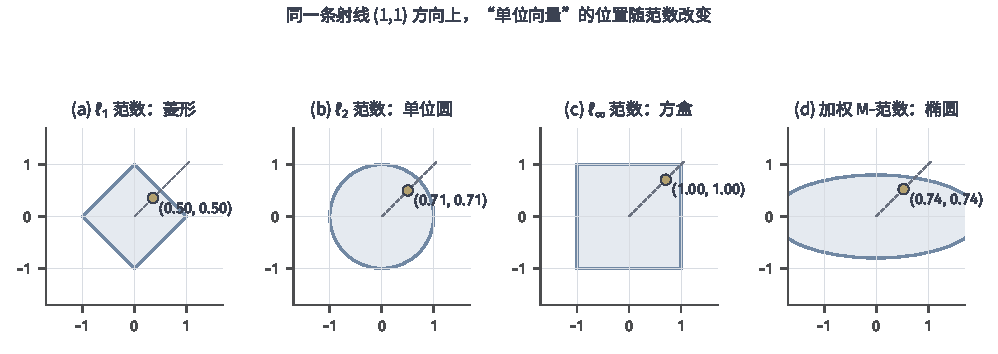
\includegraphics[width=169mm]{figures/01-mathematical-preliminaries-upper/03-linear-spaces/matplotlib/ls-norm-unit-balls/ls-norm-unit-balls.pdf}
  \caption{同一向量在不同范数下的“单位球”形状。左：$\ell_1$单位球为菱形（累加绝对偏差）；中：$\ell_2$单位球为圆（欧氏长度）；右：$\ell_\infty$单位球为正方形（最大坐标偏差）。同一个点$(1,1)$的范数依次为$2$、$\sqrt2$、$1$，单位球大小随口径而变，三者之间的倍数关系由正文的显式不等式给出。三图坐标尺度相同，为解析教学例。}
  \label{fig:ls-norm-unit-balls}
\end{figure*}

有时只关心向量的一部分信息，这时允许非零向量的大小为零，但保留齐次性与三角不等式。这样的尺度称为\term{半范数}（seminorm）。它给出的“距离”可能把不同的点判为距离为零，下面的例子说明这一点。
\begin{example}[只看第一个坐标的半范数]
\label{ex:ls-seminorm-first-coordinate}
给定：$\mathbb R^2$上的函数$p(\bm x)=|x_1|$。
验证：$p(\bm x)\geq0$；$p(c\bm x)=|cx_1|=|c|\,p(\bm x)$；$p(\bm x+\bm y)=|x_1+y_1|\leq|x_1|+|y_1|=p(\bm x)+p(\bm y)$。所以$p$满足非负性、齐次性与三角不等式。但非零向量$(0,1)^\top$满足$p\bigl((0,1)^\top\bigr)=0$，正定性不成立。
结论：$p$是半范数而不是范数。它判定$(0,0)^\top$与$(0,1)^\top$的距离为$p\bigl((0,-1)^\top\bigr)=0$，完全忽略了第二个坐标上的差别。
\end{example}
使用半范数之前，须先说明哪些差别被有意忽略。

\subsection{向量运算的性质}
\label{sec:ls-vector-operation-properties}

上一小节只给出了运算的定义；实际推导时还要知道哪些变形允许做、哪些估计一定成立。本小节按运算分组：先是加法与数乘的八条规则，再是内积的三条基本性质，最后是$p$范数满足的Hölder不等式与Minkowski不等式、欧氏范数特有的平行四边形恒等式，以及常用范数之间的比较。由内积公理推出的Cauchy--Schwarz不等式与夹角对一般内积都成立，放到第~\ref{sec:ls-inner-product-definition}节统一讨论。

\subsubsection{加法与数乘的性质}
\label{sec:ls-vector-operation-rules}

加法与数乘逐坐标定义，只用到实数的加法与乘法，所以下面每一条都可以在任一坐标上用实数运算直接验证。设$\bm u,\bm v,\bm w\in\mathbb R^d$，$a,b\in\mathbb R$。

\paragraph{加法交换律与结合律}
\[
 \bm u+\bm v=\bm v+\bm u,\qquad
 (\bm u+\bm v)+\bm w=\bm u+(\bm v+\bm w).
\]

\paragraph{零向量与相反向量}
\[
 \bm u+\bm0=\bm u,\qquad
 \bm u+(-\bm u)=\bm0.
\]

\paragraph{数乘结合律与单位数}
\[
 a(b\bm u)=(ab)\bm u,\qquad
 1\bm u=\bm u.
\]

\paragraph{分配律}
\[
 (a+b)\bm u=a\bm u+b\bm u,\qquad
 a(\bm u+\bm v)=a\bm u+a\bm v.
\]

有了这八条规则，有限次加法与数乘可以任意添加括号、交换加项次序并展开，结果不变，所以线性组合可以像多项式一样合并同类项。下一节的同形矩阵、再后面的多维数组也逐项相加与数乘，同样的验证对它们逐字成立。第~\ref{chap:linear-representation}章将看到，后面许多结论只依赖这八条规则，而不依赖对象是一列数还是一张表。

\subsubsection{内积的性质}

下面逐条验证欧氏内积满足定义~\ref{def:linear-algebra-inner-product}的三条公理。设$\bm x,\bm y,\bm z\in\mathbb R^d$，$a,b\in\mathbb R$。

\paragraph{对称性}
\[
 \langle\bm x,\bm y\rangle=\langle\bm y,\bm x\rangle,
\]
因为每一项$x_jy_j=y_jx_j$。

\paragraph{双线性}
\[
 \langle a\bm x+b\bm z,\bm y\rangle=a\langle\bm x,\bm y\rangle+b\langle\bm z,\bm y\rangle,
\]
由有限和的运算法则$\sum_j(ax_j+bz_j)y_j=a\sum_jx_jy_j+b\sum_jz_jy_j$得到；再由对称性，对第二个变量同样成立。

\paragraph{正定性}
\[
 \langle\bm x,\bm x\rangle\geq0,\qquad
 \langle\bm x,\bm x\rangle=0\iff\bm x=\bm0,
\]
因为$\langle\bm x,\bm x\rangle=\sum_jx_j^2$，而非负数之和为零时每一项都为零。

\subsubsection{范数的性质}
\label{sec:ls-norms-distances}
\label{sec:linear-algebra-distance-relations}

上一小节的$p$范数满足非负性、正定性与齐次性，这可以直接从公式读出；需要证明的是三角不等式。$p=1$时，对每个坐标用实数的$|x_j+y_j|\leq|x_j|+|y_j|$再求和即得；$p=\infty$时，同一不等式给出$|x_j+y_j|\leq\lVert\bm x\rVert_\infty+\lVert\bm y\rVert_\infty$，再对$j$取最大值即得。$1<p<\infty$时，先要建立下面的不等式，它用一对互相配合的$p$范数与$q$范数控制两个向量逐项乘积之和。

\paragraph{Hölder不等式}
\begin{theorem}[有限维Hölder不等式]
\label{thm:linear-algebra-holder}
设$1\leq p,q\leq\infty$且$1/p+1/q=1$（约定$1/\infty=0$），则$|\bm x^\top\bm y|\leq\lVert\bm x\rVert_p\lVert\bm y\rVert_q$。
\end{theorem}
\begin{proof}
先设$1<p,q<\infty$，分三步证明。

第一步，证明Young不等式：对$u,v\geq0$，
\[
 uv\leq\frac{u^p}{p}+\frac{v^q}{q}.
\]
$u=0$时左侧为零，不等式成立。$u>0$时令$t=v/u^{p-1}\geq0$。由$1/p+1/q=1$得$(p-1)q=p$，于是$v^q=t^qu^p$、$uv=tu^p$，不等式化为
\[
 u^p\Bigl(\frac1p+\frac{t^q}{q}-t\Bigr)\geq0.
\]
函数$f(t)=1/p+t^q/q-t$的导数$t^{q-1}-1$在$0<t<1$时为负、在$t>1$时为正，所以$f$在$t\geq0$上的最小值是$f(1)=1/p+1/q-1=0$，不等式成立。

第二步，在单位尺度下求和。若$\bm x$或$\bm y$为零向量，结论两侧都为零。否则令$u_j=|x_j|/\lVert\bm x\rVert_p$、$v_j=|y_j|/\lVert\bm y\rVert_q$，则$\sum_ju_j^p=\sum_jv_j^q=1$。对每个$j$用Young不等式再求和，
\[
 \sum_ju_jv_j\leq\frac1p\sum_ju_j^p+\frac1q\sum_jv_j^q=\frac1p+\frac1q=1.
\]

第三步，恢复尺度。上式两边乘以$\lVert\bm x\rVert_p\lVert\bm y\rVert_q$，再用$|\bm x^\top\bm y|\leq\sum_j|x_j||y_j|$，即得
\[
 |\bm x^\top\bm y|\leq\sum_j|x_j||y_j|\leq\lVert\bm x\rVert_p\lVert\bm y\rVert_q.
\]

端点情形直接估计。$p=1$、$q=\infty$时，
\[
 \sum_j|x_j||y_j|\leq\Bigl(\max_j|y_j|\Bigr)\sum_j|x_j|=\lVert\bm x\rVert_1\lVert\bm y\rVert_\infty;
\]
$p=\infty$、$q=1$时交换两个向量的角色。
\end{proof}
$p=q=2$时，它给出$|\bm x^\top\bm y|\leq\lVert\bm x\rVert_2\lVert\bm y\rVert_2$。第~\ref{sec:ls-inner-product-definition}节将只用内积公理，对任一内积证明同样形式的不等式，即Cauchy--Schwarz不等式。

\paragraph{Minkowski不等式}
\[
 \lVert\bm x+\bm y\rVert_p\leq\lVert\bm x\rVert_p+\lVert\bm y\rVert_p,\qquad1\leq p\leq\infty.
\]
$p=1,\infty$的情形已在本小节开头说明。下面设$1<p<\infty$，并设$\bm x+\bm y\neq\bm0$（否则左侧为零）。取$q=p/(p-1)$，则$1/p+1/q=1$。先对每个坐标用实数的三角不等式，
\[
 |x_j+y_j|^p=|x_j+y_j|^{p-1}|x_j+y_j|\leq|x_j+y_j|^{p-1}|x_j|+|x_j+y_j|^{p-1}|y_j|.
\]
记$\bm s$为坐标$s_j=|x_j+y_j|^{p-1}$的向量。由$(p-1)q=p$，
\[
 \lVert\bm s\rVert_q=\Bigl(\sum_j|x_j+y_j|^{p}\Bigr)^{1/q}=\lVert\bm x+\bm y\rVert_p^{p/q}=\lVert\bm x+\bm y\rVert_p^{p-1}.
\]
把逐坐标的不等式对$j$求和，右侧两部分分别是$\bm s$与$(|x_1|,\ldots,|x_d|)^\top$、$\bm s$与$(|y_1|,\ldots,|y_d|)^\top$的内积，各用一次Hölder不等式，得到
\[
 \lVert\bm x+\bm y\rVert_p^p\leq\lVert\bm s\rVert_q\bigl(\lVert\bm x\rVert_p+\lVert\bm y\rVert_p\bigr)
 =\lVert\bm x+\bm y\rVert_p^{p-1}\bigl(\lVert\bm x\rVert_p+\lVert\bm y\rVert_p\bigr).
\]
两边除以$\lVert\bm x+\bm y\rVert_p^{p-1}>0$即得。于是每个$p$范数都满足范数的四条要求；取$p=2$，欧氏长度满足三角不等式。

\paragraph{平行四边形恒等式}
$p$范数都满足范数的四条要求，但欧氏范数还由标准内积给出，因而多满足一条一般范数未必满足的等式：
\begin{equation}
 \lVert\bm x+\bm y\rVert_2^2+\lVert\bm x-\bm y\rVert_2^2
 =2\lVert\bm x\rVert_2^2+2\lVert\bm y\rVert_2^2.
 \label{eq:functional-parallelogram-identity}
\end{equation}
它称为\term{平行四边形恒等式}。几何上，以$\bm x,\bm y$为邻边的平行四边形，两条对角线长度的平方和等于四条边长度的平方和。证明时按前面验证的内积双线性与对称性展开，
\[
 \lVert\bm x\pm\bm y\rVert_2^2=\langle\bm x\pm\bm y,\bm x\pm\bm y\rangle=\lVert\bm x\rVert_2^2\pm2\langle\bm x,\bm y\rangle+\lVert\bm y\rVert_2^2,
\]
两式相加，交叉项$\pm2\langle\bm x,\bm y\rangle$相互抵消，即得式~\eqref{eq:functional-parallelogram-identity}。

推导只用到两点：长度由内积按式~\eqref{eq:linear-algebra-inner-product-norm}给出，内积满足双线性与对称性。所以把标准内积换成定义~\ref{def:linear-algebra-inner-product}中的任一内积，它给出的长度同样满足这一恒等式。

反过来，恒等式可以检验一个范数是否来自内积：只要某个范数在一对向量上使恒等式两侧不等，它就不可能由任何内积给出。下面的反例用这个办法检验$\ell_1$与$\ell_\infty$范数。
\begin{example}[反例：$\ell_1$与$\ell_\infty$范数不来自内积]
\label{ex:ls-l1-linf-not-inner-product}
给定：$\mathbb R^2$中的$\bm x=\bm e_1$、$\bm y=\bm e_2$，于是$\bm x+\bm y=(1,1)^\top$，$\bm x-\bm y=(1,-1)^\top$。
计算：对$\ell_1$范数，
\[
 \lVert\bm x+\bm y\rVert_1^2+\lVert\bm x-\bm y\rVert_1^2=2^2+2^2=8,\qquad
 2\lVert\bm x\rVert_1^2+2\lVert\bm y\rVert_1^2=2\cdot1^2+2\cdot1^2=4;
\]
对$\ell_\infty$范数，
\[
 \lVert\bm x+\bm y\rVert_\infty^2+\lVert\bm x-\bm y\rVert_\infty^2=1^2+1^2=2,\qquad
 2\lVert\bm x\rVert_\infty^2+2\lVert\bm y\rVert_\infty^2=4.
\]
结论：两种范数都使恒等式两侧不等。所以不存在内积使$\lVert\bm x\rVert_1=\sqrt{\langle\bm x,\bm x\rangle}$对一切$\bm x$成立，$\ell_\infty$范数同样不是由内积给出的长度。
\end{example}

\paragraph{常用范数之间的比较}
对$\bm x\in\mathbb R^d$，
\[
 \lVert\bm x\rVert_\infty\leq\lVert\bm x\rVert_2\leq\sqrt d\,\lVert\bm x\rVert_\infty,
 \qquad
 \lVert\bm x\rVert_2\leq\lVert\bm x\rVert_1\leq\sqrt d\,\lVert\bm x\rVert_2.
\]
左端两式的依据是：平方和不小于其中最大的一项，所以$\lVert\bm x\rVert_\infty^2\leq\lVert\bm x\rVert_2^2$；展开$(\sum_j|x_j|)^2$时交叉项非负，所以$\lVert\bm x\rVert_1^2\geq\sum_jx_j^2=\lVert\bm x\rVert_2^2$。右端两式的依据是：$\sum_jx_j^2\leq d\max_jx_j^2$给出$\lVert\bm x\rVert_2\leq\sqrt d\,\lVert\bm x\rVert_\infty$；把$\sum_j|x_j|$看作$(|x_1|,\ldots,|x_d|)^\top$与全$1$向量的内积，用$p=q=2$的Hölder不等式，得到$\lVert\bm x\rVert_1\leq\sqrt d\,\lVert\bm x\rVert_2$。

下面在示例~\ref{ex:ls-p-norms}的向量上核对这四个不等式。
\begin{example}[范数比较的数值核对]
\label{ex:ls-norm-comparison-check}
给定：$d=2$，$\bm x=(3,-4)^\top$；由示例~\ref{ex:ls-p-norms}，$\lVert\bm x\rVert_1=7$，$\lVert\bm x\rVert_2=5$，$\lVert\bm x\rVert_\infty=4$。
验证：
\[
 4\leq5\leq4\sqrt2\approx5.66,\qquad
 5\leq7\leq5\sqrt2\approx7.07.
\]
结论：四个不等式都成立。右端的$\sqrt2$都不能换成$1$：$\lVert\bm x\rVert_2=5$大于$\lVert\bm x\rVert_\infty=4$，$\lVert\bm x\rVert_1=7$也大于$\lVert\bm x\rVert_2=5$。
\end{example}
右端的常数随维数增大，而且一般不能改小：全$1$向量$\bm 1\in\mathbb R^d$满足$\lVert\bm 1\rVert_\infty=1$、$\lVert\bm 1\rVert_2=\sqrt d$、$\lVert\bm 1\rVert_1=d$，两个右端不等式都取等号。所以维数较大时，$\sqrt d$不能在误差预算中忽略。

本节在向量层面得到了三组工具：加法、数乘与线性组合满足的八条规则；内积及由它导出的长度与正交；由范数统一的误差口径及其间的不等式。夹角留到第~\ref{sec:ls-inner-product-definition}节，线性读取在误差预算下的最大变化（对偶范数）留到第~\ref{sec:ls-dual-norms}节。把若干向量并排放在一起，就得到下一节的矩阵。

% 第4章第2节（上）：矩阵的表示（矩阵、元素与形状，设计矩阵与贯穿例）、常见矩阵（方阵、零矩阵、对角矩阵、单位矩阵、上三角矩阵、下三角矩阵、对称矩阵、正定矩阵与半正定矩阵、置换矩阵、正交矩阵）、矩阵的运算（加法与数乘、转置、矩阵与向量的乘积、矩阵乘法、逐项乘积、逆矩阵、矩阵幂、迹、Frobenius内积、Frobenius范数、诱导矩阵范数、行列式）。运算的性质见03-matrix-properties.tex。

\section{矩阵}
\label{sec:ls-matrices}

一批样本的特征排成一张数表以后，问题随之而来：对每个样本用同一组权重求加权和，要算许多个同样形式的和，能否一次写出；两次这样的计算接连进行，能否合成一次；一次计算能否撤销，反复进行时怎样书写；一张表把单位正方形变成平行四边形时，面积放大多少；作为计算，它最多把输入放大多少倍。这些问题都以矩阵为对象。本节先规定矩阵的写法，再介绍元素分布有固定模式的几类常见矩阵，然后逐一定义矩阵的运算，最后按运算整理它们满足的性质。

与向量不同，矩阵最重要的运算不是逐项进行的加法，而是由加权求和导出的乘法。乘法的规则与实数乘法有同有异，需要逐条核对。

\subsection{矩阵的表示}
\label{sec:ls-matrix-representation}

定位向量中的一个数需要一个索引；一张数表的每个数要由所在的行与列共同确定，需要两个索引。

\paragraph{矩阵、元素与形状}
$m$行$d$列的实数表称为矩阵（matrix），记为$\bm A\in\mathbb R^{m\times d}$；第$i$行、第$j$列的元素记为$\bm A_{i,j}$，不会混淆时也写作$a_{i,j}$。$m\times d$称为矩阵的形状，行数写在列数之前。记号$\bm A_{i,:}$表示第$i$行，$\bm A_{:,j}$表示第$j$列，冒号表示该方向上的全部位置；第$j$列是一个$m$维列向量，第$i$行是一个$d$维行向量。例如在
\[
 \bm A=\begin{bmatrix}1&2&3\\4&5&6\end{bmatrix}\in\mathbb R^{2\times3}
\]
中，$\bm A_{2,1}=4$，第一行$\bm A_{1,:}=\left[\begin{smallmatrix}1&2&3\end{smallmatrix}\right]$，第三列$\bm A_{:,3}=(3,6)^\top$。

两个矩阵相等，要求形状相同且每个对应元素相等。只有一行的矩阵就是行向量，只有一列的矩阵就是列向量，所以向量可以看作矩阵的特例。

\paragraph{设计矩阵}
用矩阵记录数据时，通常让每行对应一个样本，每列对应一个特征，这样的矩阵称为设计矩阵。把示例~\ref{ex:ls-nearly-collinear-features}中两个特征的取值向量$\bm c_1,\bm c_2$并排作为两列，得到三个样本、两个特征的设计矩阵
\begin{equation}
 \bm X_{\varepsilon}
 =\begin{bmatrix}1&1\\1&1+\varepsilon\\1&1-\varepsilon\end{bmatrix}
 =\begin{bmatrix}\bm c_1&\bm c_2\end{bmatrix},
 \qquad
 \bm q=\begin{bmatrix}0\\1\\-1\end{bmatrix},
 \quad \bm c_2=\bm c_1+\varepsilon\bm q.
 \label{eq:linear-algebra-nearly-collinear-design}
\end{equation}
$|\varepsilon|$很小时，两列之差$\bm c_2-\bm c_1=\varepsilon\bm q$很短，两列几乎是同一串数；第~\ref{sec:ls-inner-product-definition}节将用夹角说明它们几乎同向。这个例子将贯穿整个线性空间部分：第~\ref{chap:linear-representation}章讨论这样两列能否充当一组记录方向，后续两章再看它怎样影响谱、求解与误差。

\subsection{常见矩阵}
\label{sec:prelim-common-matrices}

有些矩阵的元素分布有固定模式：大部分位置为零，或者主对角线两侧互相对称，或者各列彼此正交；对称矩阵中还有一类由二次型的符号刻画。这些模式会让后面的运算大为简化。本小节按元素的位置与取值逐类给出定义和例子；它们在乘法、转置、求逆下怎样表现，放到第~\ref{sec:ls-matrix-operation-properties}节讨论。

\paragraph{方阵}
行数等于列数的矩阵称为方阵（square matrix），$n\times n$方阵也称$n$阶方阵；位置$(i,i)$上的元素组成主对角线。例如$\left[\begin{smallmatrix}1&2\\3&4\end{smallmatrix}\right]$是二阶方阵，主对角元素为$1$和$4$；$2\times3$矩阵不是方阵，也没有主对角线的说法。

\paragraph{零矩阵}
全部元素都为$0$的矩阵称为零矩阵（zero matrix），记作$\bm0$。它不要求是方阵，使用时须写明形状，例如
\[
 \bm0_{2\times3}=\begin{bmatrix}0&0&0\\0&0&0\end{bmatrix}.
\]

\paragraph{对角矩阵}
主对角线以外的元素都为$0$的方阵称为对角矩阵（diagonal matrix），记为$\operatorname{diag}(d_1,\ldots,d_n)$，主对角元素本身可以为$0$。例如
\[
 \operatorname{diag}(2,0)=\begin{bmatrix}2&0\\0&0\end{bmatrix},\qquad
 \operatorname{diag}(1,-1,3)=\begin{bmatrix}1&0&0\\0&-1&0\\0&0&3\end{bmatrix}.
\]

\paragraph{单位矩阵}
主对角元素全为$1$的对角矩阵称为单位矩阵（identity matrix），记为$\bm I_n$，不必强调阶数时写作$\bm I$。它的第$j$列就是标准坐标向量$\bm e_j$。例如
\[
 \bm I_3=\begin{bmatrix}1&0&0\\0&1&0\\0&0&1\end{bmatrix}=\begin{bmatrix}\bm e_1&\bm e_2&\bm e_3\end{bmatrix}.
\]

\paragraph{上三角矩阵}
$i>j$时$\bm A_{i,j}=0$的方阵称为上三角矩阵（upper triangular matrix）：主对角线以下全为零，非零元素只可能出现在主对角线及其上方。例如
\[
 \begin{bmatrix}1&2&3\\0&4&5\\0&0&6\end{bmatrix}.
\]

\paragraph{下三角矩阵}
$i<j$时$\bm A_{i,j}=0$的方阵称为下三角矩阵（lower triangular matrix）：主对角线以上全为零。例如
\[
 \begin{bmatrix}1&0&0\\2&3&0\\4&5&6\end{bmatrix}.
\]
对角矩阵既是上三角矩阵，也是下三角矩阵。

\paragraph{对称矩阵}
满足$\bm A_{i,j}=\bm A_{j,i}$对全部$i,j$成立的方阵称为对称矩阵（symmetric matrix），它关于主对角线镜像对称；定义转置以后，这个条件写作$\bm A^\top=\bm A$。例如
\[
 \begin{bmatrix}1&2\\2&3\end{bmatrix},\qquad
 \begin{bmatrix}4&-1&0\\-1&2&5\\0&5&1\end{bmatrix}.
\]
对角矩阵都是对称矩阵。

\paragraph{正定矩阵与半正定矩阵}
$n$阶对称矩阵$\bm M$与向量$\bm x\in\mathbb R^n$给出一个数
\[
 q(\bm x)=\sum_{i=1}^n\sum_{j=1}^n m_{i,j}x_ix_j,
\]
称为$\bm M$的二次型；定义矩阵乘法以后，它写作$\bm x^\top\bm M\bm x$。

若对每个非零$\bm x$都有$q(\bm x)>0$，就称$\bm M$\term{正定}（positive definite），记作$\bm M\succ\bm0$；若只保证$q(\bm x)\geq0$对一切$\bm x$成立，就称$\bm M$\term{半正定}（positive semidefinite），记作$\bm M\succeq\bm0$。对两个同阶对称矩阵，$\bm M\succeq\bm N$表示$\bm M-\bm N\succeq\bm0$，即$\bm M$的二次型处处不小于$\bm N$的二次型；它比较的是两个二次型，不是逐个元素。

判断正定性，要看二次型能否在某个非零向量处取到零或负值。下面用配方比较两个二阶矩阵。
\begin{example}[用配方区分正定与半正定]
\label{ex:ls-pd-psd-completing-square}
给定：$\bm M=\left[\begin{smallmatrix}4&2\\2&2\end{smallmatrix}\right]$，$\bm N=\left[\begin{smallmatrix}1&1\\1&1\end{smallmatrix}\right]$。
计算：两者的二次型配方为
\[
 \begin{aligned}
 q_{\bm M}(\bm x)&=4x_1^2+4x_1x_2+2x_2^2=(2x_1+x_2)^2+x_2^2,\\
 q_{\bm N}(\bm x)&=x_1^2+2x_1x_2+x_2^2=(x_1+x_2)^2.
 \end{aligned}
\]
$q_{\bm M}$是两个平方之和，只在$2x_1+x_2=0$且$x_2=0$，即$\bm x=\bm0$时为零。$q_{\bm N}$处处非负，但在非零向量$\bm x=(1,-1)^\top$处为零。
结论：$\bm M\succ\bm0$；$\bm N\succeq\bm0$，但$\bm N$不是正定矩阵。
\end{example}

对角矩阵的二次型是$\sum_id_ix_i^2$。若全部$d_i>0$，每个非零$\bm x$都使它为正；若某个$d_i\leq0$，取$\bm x=\bm e_i$就得到$q(\bm e_i)=d_i\leq0$。所以对角矩阵正定当且仅当全部$d_i>0$，例如$\bm I_n\succ\bm0$。

正定性要对全部非零向量检查，只看元素的符号并不够，下面的反例说明这一点。
\begin{example}[反例：元素全为正的对称矩阵未必正定]
\label{ex:ls-positive-entries-not-pd}
给定：$\bm M=\left[\begin{smallmatrix}1&2\\2&1\end{smallmatrix}\right]$，四个元素都为正。
计算：它的二次型为$q(\bm x)=x_1^2+4x_1x_2+x_2^2$。取$\bm x=(1,-1)^\top$，
\[
 q(\bm x)=1^2+4\cdot1\cdot(-1)+(-1)^2=-2.
\]
结论：$q(\bm x)<0$，所以$\bm M$不是正定矩阵，也不是半正定矩阵。
\end{example}

\paragraph{置换矩阵}
把单位矩阵的各列重新排列得到的方阵称为置换矩阵（permutation matrix），它的每行、每列恰有一个$1$，其余为$0$。例如
\[
 \begin{bmatrix}0&1\\1&0\end{bmatrix}=\begin{bmatrix}\bm e_2&\bm e_1\end{bmatrix},\qquad
 \begin{bmatrix}0&0&1\\1&0&0\\0&1&0\end{bmatrix}=\begin{bmatrix}\bm e_2&\bm e_3&\bm e_1\end{bmatrix}.
\]
第一个矩阵乘在平面向量上会交换两个坐标，这一点在定义矩阵乘法以后验证。

\paragraph{正交矩阵}
\phantomsection
\label{sec:ls-orthogonal-matrices}
若$n$阶方阵$\bm Q$的各列都是单位向量，并且两两正交（在上一节欧氏内积的意义下），就称它为\term{正交矩阵}（orthogonal matrix）。单位矩阵和置换矩阵都是正交矩阵，因为它们的列是互不相同的标准坐标向量。

下面检验平面旋转矩阵满足这一定义，并说明只有各列两两正交还不够。
\begin{example}[平面旋转是正交矩阵]
\label{ex:ls-rotation-orthogonal}
给定：任一实数$\phi$对应的平面旋转矩阵
\[
 \bm R_\phi=\begin{bmatrix}\cos\phi&-\sin\phi\\\sin\phi&\cos\phi\end{bmatrix},
\]
以及对角矩阵$\operatorname{diag}(2,1)$。
验证：$\bm R_\phi$两列的长度与内积分别为
\[
 \sqrt{\cos^2\phi+\sin^2\phi}=1,\qquad
 \cos\phi\cdot(-\sin\phi)+\sin\phi\cdot\cos\phi=0.
\]$\operatorname{diag}(2,1)$的两列$(2,0)^\top$与$(0,1)^\top$内积为零，但第一列长度为$2$。
结论：$\bm R_\phi$是正交矩阵；$\operatorname{diag}(2,1)$的各列两两正交，却不是正交矩阵，因为正交矩阵还要求每列长度为$1$。
\end{example}
正交矩阵与转置、乘法、求逆、行列式和范数的关系，分别在第~\ref{sec:ls-matrix-operation-properties}节相应运算的性质中给出。

\subsection{矩阵的运算}
\label{sec:ls-matrix-operations}
\label{sec:ls-multiplication}

矩阵的运算按来源可以分成几类。加法与数乘沿用向量的逐项规则，转置只改变元素的位置。矩阵与向量的乘积一次写出许多加权和，矩阵乘法、逆矩阵与矩阵幂都以它为基础。逐项乘积是另一种“相乘”，它不汇总任何索引。迹、Frobenius内积、矩阵范数与行列式则把矩阵读成一个数。本小节按这个顺序逐一给出计算方法，各运算满足的规则集中放在下一小节。

\subsubsection{加法与数乘}

同形矩阵$\bm A,\bm B\in\mathbb R^{m\times n}$逐项相加减，数乘把每个元素乘以同一个实数$c$：
\[
 (\bm A\pm\bm B)_{i,j}=a_{i,j}\pm b_{i,j},\qquad
 (c\bm A)_{i,j}=ca_{i,j},
\]
结果形状不变。下面是一组二阶矩阵的算例。
\begin{example}[矩阵的加法、减法与数乘]
\label{ex:ls-matrix-addition-scaling}
给定：$\bm A=\left(\begin{smallmatrix}1&2\\3&4\end{smallmatrix}\right)$，$\bm B=\left(\begin{smallmatrix}0&1\\-1&2\end{smallmatrix}\right)$，$c=3$。
计算：逐项运算，
\[
 \bm A+\bm B=\begin{pmatrix}1&3\\2&6\end{pmatrix},\qquad
 \bm A-\bm B=\begin{pmatrix}1&1\\4&2\end{pmatrix},\qquad
 3\bm A=\begin{pmatrix}3&6\\9&12\end{pmatrix}.
\]
例如$\bm A+\bm B$的$(2,1)$元为$3+(-1)=2$，$\bm A-\bm B$的$(2,1)$元为$3-(-1)=4$。
结论：三个结果都是$2\times2$矩阵，每个元素只用到输入在同一位置上的元素。
\end{example}
与向量一样，两个矩阵能够相加，要求形状相同、对应位置含义相同；即使元素总数恰好相同，$2\times3$矩阵与$3\times2$矩阵也不能相加。同形矩阵的线性组合按同样方式定义。

\subsubsection{转置}

转置交换行与列：$\bm A\in\mathbb R^{m\times n}$的元素$a_{i,j}$原样搬到$\bm A^\top\in\mathbb R^{n\times m}$的位置$(j,i)$，
\[
 (\bm A^\top)_{j,i}=\bm A_{i,j}.
\]
形状交换而数值不变，原来的第$i$行成为第$i$列。把列向量看作$d\times1$矩阵，这一定义与上一节向量的转置一致。下面的例子显示行怎样变成列。
\begin{example}[转置一个$2\times3$矩阵]
\label{ex:ls-transpose-two-by-three}
给定：$\bm A=\left[\begin{smallmatrix}1&2&3\\4&5&6\end{smallmatrix}\right]\in\mathbb R^{2\times3}$。
计算：把每个$(i,j)$元搬到$(j,i)$位置，
\[
 \bm A^\top=\begin{bmatrix}1&4\\2&5\\3&6\end{bmatrix}\in\mathbb R^{3\times2}.
\]
结论：$\bm A$的第一行$(1,2,3)$成为$\bm A^\top$的第一列，第二行$(4,5,6)$成为第二列。
\end{example}

\subsubsection{矩阵与向量的乘积}
\label{sec:prelim-matrix-records-prediction}

设$n$次观测的输入排成设计矩阵$\bm X\in\mathbb R^{n\times d}$，权重排成$\bm w\in\mathbb R^d$。线性预测对每次观测计算同一种加权和$\sum_j x_{i,j}w_j$，即$\bm X$的第$i$行与$\bm w$的内积。矩阵与向量的乘积把这$n$个加权和一次写出：对$\bm A\in\mathbb R^{m\times d}$与$\bm u\in\mathbb R^d$，$\bm A\bm u$是$m$维列向量，
\begin{equation}
 (\bm A\bm u)_i=\sum_{j=1}^d\bm A_{i,j}u_j,\qquad i=1,\ldots,m.
 \label{eq:prelim-matrix-prediction}
\end{equation}
矩阵的列数必须等于向量的维数。同一个结果有两种算法：
\begin{itemize}
 \item 按行算：输出的第$i$个坐标是第$i$行与$\bm u$的内积；
 \item 按列算：同一个$u_j$乘的恰好是第$j$列的全部元素，所以
 \[
  \bm A\bm u=u_1\bm A_{:,1}+u_2\bm A_{:,2}+\cdots+u_d\bm A_{:,d},
 \]
 乘积是矩阵各列以$u_j$为系数的线性组合。
\end{itemize}
特别地，按列算时，$\bm e_j$只有第$j$个系数为$1$，所以$\bm A\bm e_j=\bm A_{:,j}$：乘第$j$个标准坐标向量就取出第$j$列。

下面用一个二阶例子核对两种算法给出同一结果。
\begin{example}[按行与按列计算矩阵与向量的乘积]
\label{ex:ls-matrix-vector-rows-columns}
给定：$\bm A=\left[\begin{smallmatrix}2&1\\0&3\end{smallmatrix}\right]$，$\bm u=(1,1)^\top$。
计算：按行算，每个坐标是一行与$\bm u$的内积；按列算，结果是两列以$u_1=u_2=1$为系数的线性组合：
\[
 \bm A\bm u
 =\begin{bmatrix}2\cdot1+1\cdot1\\0\cdot1+3\cdot1\end{bmatrix}
 =\begin{bmatrix}3\\3\end{bmatrix},
 \qquad
 \bm A\bm u=1\begin{bmatrix}2\\0\end{bmatrix}+1\begin{bmatrix}1\\3\end{bmatrix}
 =\begin{bmatrix}3\\3\end{bmatrix}.
\]
结论：两种算法都得到$\bm A\bm u=(3,3)^\top$。
\end{example}

用于数据时，矩阵与向量的乘积一次给出全部样本的预测。下面以一次函数为例。
\begin{example}[用矩阵与向量的乘积计算一次函数的取值]
\label{ex:ls-affine-predictions}
给定：要在$x=1,2,3$处计算$ax+b$，取
\[
 \bm X=\begin{pmatrix}1&1\\2&1\\3&1\end{pmatrix},\qquad
 \bm w=\begin{pmatrix}a\\b\end{pmatrix}.
\]
计算：按行算，
\[
 \bm X\bm w=\begin{pmatrix}1\cdot a+1\cdot b\\2\cdot a+1\cdot b\\3\cdot a+1\cdot b\end{pmatrix}=\begin{pmatrix}a+b\\2a+b\\3a+b\end{pmatrix}.
\]
结论：$\bm X\bm w$的三个坐标正是三处的函数值。第二列全为$1$，使每行都加上同一个截距$b$。
\end{example}

观测输出排成$\bm y$以后，全部残差就是$\bm X\bm w-\bm y$，平方误差总和写成
\[
 \sum_{i=1}^n\left(\sum_{j=1}^d x_{i,j}w_j-y_i\right)^2
 =\lVert\bm X\bm w-\bm y\rVert_2^2.
\]
左侧逐个样本求加权和、减去观测、平方后相加；右侧把同样的计算写成残差向量长度的平方。对贯穿例，按列算得$\bm X_\varepsilon\bm w=w_1\bm c_1+w_2\bm c_2$：预测是两个特征取值向量的线性组合。

\subsubsection{矩阵乘法}
\phantomsection
\label{sec:prelim-linear-actions-composition}

对$\bm A\in\mathbb R^{m\times d}$与$\bm B\in\mathbb R^{d\times k}$，乘积$\bm A\bm B\in\mathbb R^{m\times k}$为
\begin{equation}
 (\bm A\bm B)_{i,j}=\sum_{\ell=1}^d\bm A_{i,\ell}\bm B_{\ell,j}.
 \label{eq:prelim-matrix-composition}
\end{equation}
左矩阵的列数必须等于右矩阵的行数；第$(i,j)$项取左矩阵的第$i$行与右矩阵的第$j$列，逐项相乘后相加。下面逐项计算一个二阶乘积。
\begin{example}[二阶矩阵的乘积]
\label{ex:ls-matrix-product-2x2}
给定：$\bm A=\left(\begin{smallmatrix}1&1\\0&1\end{smallmatrix}\right)$，$\bm B=\left(\begin{smallmatrix}1&0\\0&2\end{smallmatrix}\right)$。
计算：第$(i,j)$项是$\bm A$的第$i$行与$\bm B$的第$j$列的内积，
\[
 \bm A\bm B
 =\begin{pmatrix}1\cdot1+1\cdot0&1\cdot0+1\cdot2\\0\cdot1+1\cdot0&0\cdot0+1\cdot2\end{pmatrix}
 =\begin{pmatrix}1&2\\0&2\end{pmatrix}.
\]
结论：$\bm A\bm B=\left(\begin{smallmatrix}1&2\\0&2\end{smallmatrix}\right)$，形状为$2\times2$。
\end{example}
$\bm B$只有一列时，式~\eqref{eq:prelim-matrix-composition}就是式~\eqref{eq:prelim-matrix-prediction}。两个向量的内积$\bm x^\top\bm y$是$1\times d$与$d\times1$矩阵的乘积，结果是$1\times1$矩阵，我们把它与它唯一的元素等同看待。

这个定义来自两次加权求和的接连进行。设$\bm x\in\mathbb R^k$，$\bm y=\bm B\bm x$、$\bm z=\bm A\bm y$，即先用$\bm B$再用$\bm A$，这是第~\ref{sec:prelim-map-operations}节意义下两个函数的复合。逐坐标代入并交换有限求和的次序，
\begin{equation}
 z_i=\sum_{\ell=1}^d a_{i,\ell}y_\ell
 =\sum_{\ell=1}^d a_{i,\ell}\sum_{j=1}^k b_{\ell,j}x_j
 =\sum_{j=1}^k\left(\sum_{\ell=1}^d a_{i,\ell}b_{\ell,j}\right)x_j,
 \label{eq:linear-algebra-matrix-product}
\end{equation}
括号中的数正是$(\bm A\bm B)_{i,j}$。所以$(\bm A\bm B)\bm x=\bm A(\bm B\bm x)$：直接用乘积作用，等于先用$\bm B$、再用$\bm A$作用。被求和的公共维数$d$就是被消去的中间结果$\bm y$的维数。

\subsubsection{逐项乘积}
\label{sec:ls-hadamard-product}

矩阵乘法汇总共同索引；另一种常用的“乘法”不汇总任何索引，只把两个同形数组在对应位置配对。设$\bm A,\bm B\in\mathbb R^{m\times n}$，\term{逐元素乘积}（Hadamard product）记作$\bm A\odot\bm B$，
\begin{equation}
 (\bm A\odot\bm B)_{i,j}=a_{i,j}b_{i,j},
 \label{eq:ls-hadamard}
\end{equation}
输出仍是$m\times n$。同维向量和更高阶的同形数组也按同样的方式逐项相乘。

同样两个矩阵，用两种乘法得到的结果完全不同，下面的例子说明这一点。
\begin{example}[逐项乘积与矩阵乘积的对比]
\label{ex:ls-hadamard-vs-matrix-product}
给定：$\bm A=\left[\begin{smallmatrix}1&2\\3&4\end{smallmatrix}\right]$，$\bm B=\left[\begin{smallmatrix}0&1\\1&0\end{smallmatrix}\right]$。
计算：
\[
 \begin{aligned}
 \bm A\odot\bm B&=\begin{bmatrix}1\cdot0&2\cdot1\\3\cdot1&4\cdot0\end{bmatrix}=\begin{bmatrix}0&2\\3&0\end{bmatrix},\\
 \bm A\bm B&=\begin{bmatrix}1\cdot0+2\cdot1&1\cdot1+2\cdot0\\3\cdot0+4\cdot1&3\cdot1+4\cdot0\end{bmatrix}=\begin{bmatrix}2&1\\4&3\end{bmatrix}.
 \end{aligned}
\]
结论：逐项乘积把$\bm B$为零的位置置零，矩阵乘积则交换了$\bm A$的两列；两个结果在每个位置上都不同。
\end{example}
固定掩码$\bm M$后，$\bm X\mapsto\bm M\odot\bm X$把$\bm M$为零的位置置零、把其余位置按系数缩放，适合表达“挑选或调制另一个数组”。

\subsubsection{逆矩阵}
\label{sec:prelim-inverse-matrices}

对$n$阶方阵$\bm A$，若存在$n$阶方阵$\bm B$满足
\[
 \bm A\bm B=\bm B\bm A=\bm I_n,
\]
就称$\bm A$可逆，$\bm B$为\term{逆矩阵}（inverse matrix），记作$\bm A^{-1}$。逆矩阵撤销乘$\bm A$的效果。$\bm A$可逆时，若$\bm A\bm x=\bm y$，两边左乘$\bm A^{-1}$得$\bm x=\bm A^{-1}\bm y$，所以方程至多有一个解；反过来，$\bm x=\bm A^{-1}\bm y$满足$\bm A\bm x=\bm A\bm A^{-1}\bm y=\bm y$。所以方程$\bm A\bm x=\bm y$有唯一解$\bm x=\bm A^{-1}\bm y$。

逆矩阵若存在则唯一：若$\bm B,\bm C$都满足条件，则$\bm B=\bm B(\bm A\bm C)=(\bm B\bm A)\bm C=\bm C$，这里用到下一小节的结合律。因此记号$\bm A^{-1}$不会有歧义。

怎样求逆取决于矩阵的结构。下面从最简单的对角矩阵开始，依次给出二阶方阵的公式与一般方阵的做法。

\paragraph{对角矩阵的逆}
每个$d_i\neq0$时逐个取倒数：
\[
 \operatorname{diag}(d_1,\ldots,d_n)^{-1}=\operatorname{diag}(1/d_1,\ldots,1/d_n).
\]
两个对角矩阵相乘时对角元逐个相乘（下一小节验证），所以两侧乘积都是$\bm I_n$。例如$\operatorname{diag}(2,1)^{-1}=\operatorname{diag}(1/2,1)$。若某个$d_i=0$，左乘$\bm D=\operatorname{diag}(d_1,\ldots,d_n)$把任何$\bm B$的第$i$行乘以$d_i$，所以$\bm D\bm B$的第$i$行是$\bm0$，不可能等于$\bm I_n$的第$i$行；这时$\bm D$不可逆。

\paragraph{二阶方阵的逆}
$ad-bc\neq0$时，
\[
 \begin{pmatrix}a&b\\c&d\end{pmatrix}^{-1}=\frac1{ad-bc}\begin{pmatrix}d&-b\\-c&a\end{pmatrix}.
\]
直接相乘即可验证两侧乘积都是$\bm I_2$：例如左上元素为$(ad-bc)/(ad-bc)=1$，右上元素为$(-ab+ba)/(ad-bc)=0$。分母$ad-bc$正是后面的二阶行列式。

\paragraph{一般方阵的逆}
一般方阵没有这样简短的公式，可以通过解方程求逆：对任意$\bm y$解$\bm A\bm x=\bm y$，把$\bm x$写成$\bm y$各坐标的线性组合，系数排成的矩阵就是$\bm A^{-1}$。下面用一个二阶例子演示，并与二阶公式对照。
\begin{example}[解方程求逆]
\label{ex:ls-inverse-by-solving}
给定：$\bm A=\left[\begin{smallmatrix}2&1\\0&3\end{smallmatrix}\right]$。
计算：方程$\bm A\bm x=\bm y$即$y_1=2x_1+x_2$、$y_2=3x_2$。由第二式得$x_2=y_2/3$，代入第一式得$x_1=(y_1-x_2)/2=y_1/2-y_2/6$。把系数排成矩阵，
\[
 \bm A^{-1}=\begin{bmatrix}1/2&-1/6\\0&1/3\end{bmatrix}.
\]
用二阶公式核对：$ad-bc=2\cdot3-1\cdot0=6$，公式给出$\frac16\left[\begin{smallmatrix}3&-1\\0&2\end{smallmatrix}\right]$，与上式相同。
结论：右上角的$-1/6$不是原元素$1$的倒数。一般矩阵把各个坐标掺在一起，逆矩阵要作为整体求出，不能逐个元素取倒数。
\end{example}
这种逐个消去未知量的做法，第~\ref{sec:ls-direct-methods}节系统化为消元法。哪些方阵可逆，第~\ref{sec:ls-injective-surjective-invertible}节用零空间与秩回答，第~\ref{sec:ls-determinant-invertibility}节再给出行列式判据。

\paragraph{单侧逆}
矩形矩阵不能有双侧的逆，但可能只从一侧抵消。对$\bm A\in\mathbb R^{m\times d}$，满足$\bm L\bm A=\bm I_d$的$\bm L\in\mathbb R^{d\times m}$称为左逆，满足$\bm A\bm R=\bm I_m$的$\bm R\in\mathbb R^{d\times m}$称为右逆。有左逆时，若$\bm A\bm x=\bm y$有解，两边左乘$\bm L$得$\bm x=\bm L\bm y$，所以解只能是$\bm L\bm y$。有右逆时，$\bm A(\bm R\bm y)=\bm I_m\bm y=\bm y$，所以$\bm x=\bm R\bm y$总是一个解。

与方阵的逆不同，单侧逆一般不唯一，下面的例子说明这一点。
\begin{example}[反例：左逆不唯一]
\label{ex:ls-left-inverse-not-unique}
给定：$\bm A=(1,0)^\top\in\mathbb R^{2\times1}$，以及任意实数$c$。
验证：取$\bm L=(1,c)\in\mathbb R^{1\times2}$，则$\bm L\bm A=1\cdot1+c\cdot0=1=\bm I_1$。
结论：每个$c$都给出$\bm A$的一个左逆，所以$\bm A$的左逆有无穷多个。
\end{example}
矩形矩阵何时有左逆或右逆，第~\ref{chap:linear-representation}章用核与像回答；第~\ref{chap:linear-equations-and-optimization}章讨论怎样实际求解，以及多解时选哪一个。

\subsubsection{矩阵幂}
\label{sec:ls-matrix-power-rules}

定常迭代$\bm x^{(k+1)}=\bm A\bm x^{(k)}$每一步都乘同一个$\bm A$。对$d$阶方阵，$\bm A^k$定义为$k$个$\bm A$连乘（$k\geq1$），并规定$\bm A^0=\bm I_d$；$\bm A$可逆时再定义负幂$\bm A^{-k}=(\bm A^{-1})^k$。于是迭代的第$k$步是$\bm x^{(k)}=\bm A^k\bm x^{(0)}$。矩形矩阵不能与自身相乘，所以没有幂。

幂是反复的矩阵乘法，不是逐元素乘方，下面的例子说明两者的差别。
\begin{example}[矩阵的平方不是逐元素平方]
\label{ex:ls-matrix-square-shear}
给定：$\bm A=\left(\begin{smallmatrix}1&1\\0&1\end{smallmatrix}\right)$。
计算：
\[
 \bm A^2=\begin{pmatrix}1&1\\0&1\end{pmatrix}\begin{pmatrix}1&1\\0&1\end{pmatrix}
 =\begin{pmatrix}1\cdot1+1\cdot0&1\cdot1+1\cdot1\\0\cdot1+1\cdot0&0\cdot1+1\cdot1\end{pmatrix}
 =\begin{pmatrix}1&2\\0&1\end{pmatrix}.
\]
结论：右上角的元素变为$2$，而逐元素平方会得到$1^2=1$；继续相乘，右上角每次增加$1$。
\end{example}

两类幂关系经常出现。满足$\bm A^2=\bm A$的方阵称为\term{幂等}（idempotent）矩阵，乘一次与乘多次效果相同。存在正整数$s$使$\bm N^s=\bm0$的方阵称为\term{幂零}（nilpotent）矩阵。下面各举一例。
\begin{example}[幂等矩阵与幂零矩阵]
\label{ex:ls-idempotent-nilpotent}
给定：$\bm P=\operatorname{diag}(1,0)$，$\bm N=\left(\begin{smallmatrix}0&1\\0&0\end{smallmatrix}\right)$。
计算：对$\bm u\in\mathbb R^2$，$\bm P\bm u=(u_1,0)^\top$只保留第一个坐标，再作用一次结果不变，所以$\bm P^2=\bm P$。$\bm N\bm u=(u_2,0)^\top$把第二个坐标移到第一个位置、把第二个位置清零；再作用一次得$\bm N(u_2,0)^\top=(0,0)^\top$。直接相乘也得到
\[
 \bm N^2=\begin{pmatrix}0&1\\0&0\end{pmatrix}\begin{pmatrix}0&1\\0&0\end{pmatrix}=\begin{pmatrix}0&0\\0&0\end{pmatrix}.
\]
结论：$\bm P$是幂等矩阵；$\bm N\neq\bm0$，却满足$\bm N^2=\bm0$，是幂零矩阵。
\end{example}
$\bm A^k$在$k$很大时是什么样子，很难从元素看出，第~\ref{chap:linear-analysis}章借助特征向量回答。

\subsubsection{迹}
\label{sec:prelim-matrix-trace}

$n$阶方阵的\term{迹}（trace）是主对角元素之和：
\[
 \operatorname{tr}(\bm A)=\sum_{i=1}^n A_{i,i}.
\]
例如$\operatorname{tr}\left(\begin{smallmatrix}1&2\\3&4\end{smallmatrix}\right)=1+4=5$，而这个矩阵全部元素之和是$10$。迹只对方阵定义，只累加对角元。

\subsubsection{Frobenius内积}

把同形矩阵的$mn$个元素看作有限个坐标，照搬欧氏内积，就得到同形矩阵之间的\term{Frobenius内积}：对$\bm A,\bm B\in\mathbb R^{m\times n}$，
\[
 \langle\bm A,\bm B\rangle_{\mathrm F}=\sum_{i=1}^m\sum_{j=1}^na_{i,j}b_{i,j},
\]
即逐项相乘后全部相加，也就是$\bm A\odot\bm B$全部元素之和。下面沿用逐项乘积一例中的两个矩阵。
\begin{example}[Frobenius内积的计算]
\label{ex:ls-frobenius-inner-product}
给定：$\bm A=\left(\begin{smallmatrix}1&2\\3&4\end{smallmatrix}\right)$，$\bm B=\left(\begin{smallmatrix}0&1\\1&0\end{smallmatrix}\right)$。
计算：
\[
 \langle\bm A,\bm B\rangle_{\mathrm F}=1\cdot0+2\cdot1+3\cdot1+4\cdot0=5.
\]
结论：结果等于示例~\ref{ex:ls-hadamard-vs-matrix-product}中$\bm A\odot\bm B$的元素之和$0+2+3+0=5$。
\end{example}

Frobenius内积满足定义~\ref{def:linear-algebra-inner-product}的三条公理：它对两个变量分别线性；交换两个矩阵不改变各项乘积，因而对称；$\langle\bm A,\bm A\rangle_{\mathrm F}=\sum_{i,j}a_{i,j}^2$非负，并且只在$\bm A=\bm0$时为零。这正是把$mn$个元素看作坐标时欧氏内积的三条性质，所以它确实是同形矩阵上的一个内积，向量一节由公理得到的结论对它都成立。

\subsubsection{Frobenius范数}
\label{sec:ls-frobenius-norm}

矩阵的“大小”有两种口径。第一种把矩阵当作数表，由Frobenius内积给出Frobenius范数
\[
 \lVert\bm A\rVert_{\mathrm F}=\sqrt{\langle\bm A,\bm A\rangle_{\mathrm F}}=\left(\sum_{i,j}a_{i,j}^2\right)^{1/2}.
\]
例如$\lVert\left(\begin{smallmatrix}1&2\\3&4\end{smallmatrix}\right)\rVert_{\mathrm F}=\sqrt{1+4+9+16}=\sqrt{30}$。它就是把$mn$个元素排成一列以后的$2$范数，所以由Minkowski不等式（$p=2$）满足范数的四条要求。

Frobenius范数也可以按作用来读。由$\bm A\bm e_j=\bm A_{:,j}$，
\[
 \lVert\bm A\rVert_{\mathrm F}^2=\sum_j\lVert\bm A_{:,j}\rVert_2^2=\sum_j\lVert\bm A\bm e_j\rVert_2^2,
\]
它是全部标准坐标输入所产生的输出平方和，而不是某一个最坏输入的放大。

需要先分组再汇总时，还可以用混合范数，例如以行为组的$\lVert\bm A\rVert_{p,q}=(\sum_i\lVert\bm A_{i,:}\rVert_p^q)^{1/q}$：内层的$p$范数衡量每组的大小，外层的$q$范数汇总各组。

\subsubsection{诱导矩阵范数}
\label{sec:ls-matrix-norms}
\label{sec:ch06-map-comparison}
\label{sec:matrix-analysis-norms-effective-rank}

第二种口径把矩阵当作计算$\bm x\mapsto\bm A\bm x$，问它最多把输入放大多少倍；误差分析更关心这一种。
\begin{definition}[由向量范数诱导的矩阵范数]
\label{def:matrix-analysis-induced-norm}
给定输入范数$\lVert\cdot\rVert_\alpha$和输出范数$\lVert\cdot\rVert_\beta$，\term{诱导矩阵范数}（induced matrix norm）为
\[
 \lVert\bm A\rVert_{\alpha\to\beta}
 =\sup_{\bm x\neq0}\frac{\lVert\bm A\bm x\rVert_\beta}{\lVert\bm x\rVert_\alpha}.
\]
两端采用同一类$p$范数时简写为$\lVert\bm A\rVert_p$。
\end{definition}
由定义，对每个$\bm x$都有$\lVert\bm A\bm x\rVert_\beta\leq\lVert\bm A\rVert_{\alpha\to\beta}\lVert\bm x\rVert_\alpha$，而且诱导范数是使这一不等式对全部$\bm x$成立的最小常数。

三种常用的诱导范数中，前两种有直接的算法：
\[
 \lVert\bm A\rVert_1=\max_j\sum_i|a_{i,j}|,\qquad
 \lVert\bm A\rVert_\infty=\max_i\sum_j|a_{i,j}|,
\]
即最大绝对列和与最大绝对行和，推导放在下一小节。第三种是诱导$2$范数，也称\term{谱范数}（spectral norm），$\lVert\bm A\rVert_2=\sup_{\lVert\bm x\rVert_2=1}\lVert\bm A\bm x\rVert_2$，它的计算要用到第~\ref{sec:ls-svd}节的奇异值。

下面在同一个矩阵上比较两种诱导范数与Frobenius范数。
\begin{example}[同一矩阵在不同口径下的大小]
\label{ex:ls-matrix-norms-shear}
给定：$\bm A=\left[\begin{smallmatrix}1&1\\0&1\end{smallmatrix}\right]$。
计算：两列的绝对值之和分别为$1+0=1$与$1+1=2$，两行的绝对值之和分别为$1+1=2$与$0+1=1$，全部元素的平方和为$1+1+0+1=3$。所以
\[
 \lVert\bm A\rVert_1=\max\{1,2\}=2,\qquad
 \lVert\bm A\rVert_\infty=\max\{2,1\}=2,\qquad
 \lVert\bm A\rVert_{\mathrm F}=\sqrt3.
\]
结论：不同口径给出的数值不必相同。
\end{example}
图~\ref{fig:ls-induced-norm-action}画出谱范数的几何意义：单位圆被$\bm A$拉成椭圆，椭圆最长半轴的长度就是最大放大倍数。
\begin{figure*}[htbp]
  \centering
  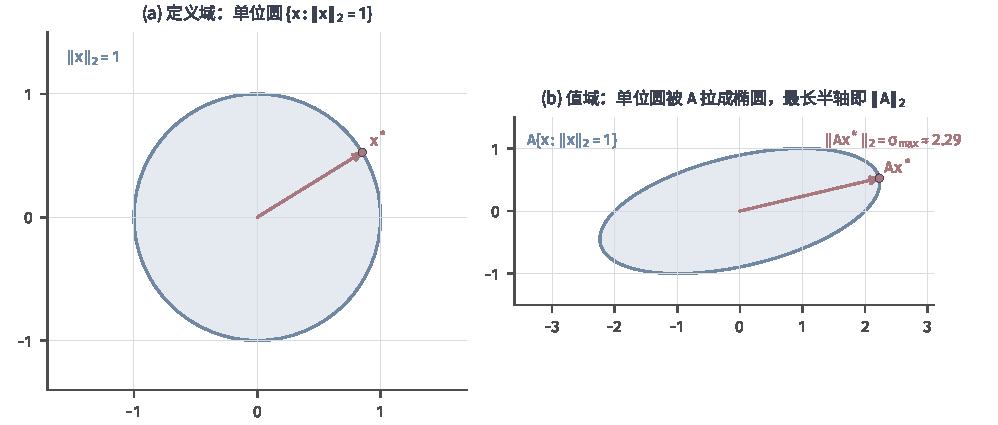
\includegraphics[width=169mm]{figures/01-mathematical-preliminaries-upper/03-linear-spaces/matplotlib/ls-induced-norm-action/ls-induced-norm-action.pdf}
  \caption{诱导矩阵范数衡量最坏放大倍数。左：单位圆$\lVert\bm x\rVert_2=1$；中：同一线性作用$\bm A$把单位圆映成椭圆；右：椭圆上最长的轴给出$\lVert\bm A\rVert_2=\max_{\lVert\bm x\rVert_2=1}\lVert\bm A\bm x\rVert_2$，箭头指示最大放大方向。数值由$\bm A$的教学构造直接得到，是解析例。}
  \label{fig:ls-induced-norm-action}
\end{figure*}

\subsubsection{行列式}
\phantomsection
\label{sec:ls-exterior-determinants}
\label{sec:linear-algebra-scalar-readouts}

一张方阵把单位正方形变成平行四边形、把单位立方体变成平行多面体时，面积或体积放大多少倍？平行四边形的面积不能由两条边的长度直接算出，它还取决于两个向量的相对方向；若再记录定向，交换两个向量的次序会使有向面积变号。下面先建立记录有向体积的外积，再由它得到行列式和它的计算公式。

\paragraph{外积}
对$\mathbb R^d$中的$k$个向量$\bm v_1,\ldots,\bm v_k$，它们的\term{外积}（exterior product，又称\term{楔积}wedge product）$\bm v_1\wedge\cdots\wedge\bm v_k$按两条规则计算。
\begin{itemize}
 \item 多线性：对每个因子分别保持线性组合，即把某个$\bm v_i$换成$a\bm u+b\bm w$时，整个楔积等于$a(\cdots\wedge\bm u\wedge\cdots)+b(\cdots\wedge\bm w\wedge\cdots)$，其余因子不动。
 \item 交替性：交换相邻两个因子，楔积变号，
 \[
  \cdots\wedge\bm v_i\wedge\bm v_j\wedge\cdots
  =-\cdots\wedge\bm v_j\wedge\bm v_i\wedge\cdots.
 \]
\end{itemize}

两条规则先给出两个推论。第一，含有两个相同因子的楔积为零：两个相同因子相邻时，交换它们不改变楔积，却使它变号，所以它等于自身的相反数，只能为零；两个相同因子不相邻时，先用相邻交换把它们移到一起，只改变符号，结论不变。第二，若某个因子是其余因子的线性组合，把这个因子按组合代入并由多线性展开，每一项都含有两个相同因子，所以整个楔积为零。

由此可以确定楔积的一般形状。设$v_{j,i}$是$\bm v_j$的第$i$个坐标，把每个$\bm v_j=\sum_i v_{j,i}\bm e_i$代入并展开，含重复下标的项为零；其余各项按交替性把下标排成递增次序，只改变符号。所以每个楔积都是基楔积$\bm e_{i_1}\wedge\cdots\wedge\bm e_{i_k}$（$i_1<\cdots<i_k$）的线性组合，这样的基楔积共有$\binom{d}{k}$个。$k>d$时，每一项都必然含有重复下标，所以楔积恒为零。

对$\{1,\ldots,k\}$上的一般排列$\pi$，可以反复交换相邻的两个因子，把$\bm v_{\pi(1)}\wedge\cdots\wedge\bm v_{\pi(k)}$排回$\bm v_1\wedge\cdots\wedge\bm v_k$。记$N(\pi)$为$\pi$的逆序对数，即满足$i<j$而$\pi(i)>\pi(j)$的索引对数。每次交换一对相邻且次序颠倒的因子，逆序对数恰好减少$1$，所以恰好经过$N(\pi)$次交换就排好，每次交换变号一次，得到
\[
 \bm v_{\pi(1)}\wedge\cdots\wedge\bm v_{\pi(k)}
 =\operatorname{sgn}(\pi)\,\bm v_1\wedge\cdots\wedge\bm v_k,
 \qquad
 \operatorname{sgn}(\pi)=(-1)^{N(\pi)}.
\]

\paragraph{有向面积与有向体积}
在$\mathbb R^2$中按两条规则展开，
\[
 \bm u\wedge\bm v
 =(u_1\bm e_1+u_2\bm e_2)\wedge(v_1\bm e_1+v_2\bm e_2)
 =(u_1v_2-u_2v_1)\,\bm e_1\wedge\bm e_2,
\]
其中用到$\bm e_1\wedge\bm e_1=\bm e_2\wedge\bm e_2=0$与$\bm e_2\wedge\bm e_1=-\bm e_1\wedge\bm e_2$。系数$u_1v_2-u_2v_1$是$\bm u,\bm v$张成的平行四边形的有向面积：绝对值是面积，符号是定向。

下面用三组向量观察有向面积的数值与符号。
\begin{example}[平面上的有向面积]
\label{ex:ls-oriented-area}
给定：三组有序向量对：$\bm u=(1,0)^\top$与$\bm v=(1,1)^\top$；交换次序后的$\bm v$与$\bm u$；共线的$(1,1)^\top$与$(2,2)^\top$。
计算：按系数公式$u_1v_2-u_2v_1$，三组依次得到
\[
 1\cdot1-0\cdot1=1,\qquad
 1\cdot0-1\cdot1=-1,\qquad
 1\cdot2-1\cdot2=0.
\]
结论：第一组张成面积为$1$的平行四边形；交换次序后面积不变而定向翻转，所以符号变负；共线的两个向量张成的平行四边形退化成线段，有向面积为$0$。
\end{example}
由上面的计数，$\mathbb R^3$中三个向量的楔积只是基楔积$\bm e_1\wedge\bm e_2\wedge\bm e_3$的倍数。这个系数的绝对值是三个向量张成的平行六面体的体积，带符号时称为\term{有向体积}。

\paragraph{行列式的定义}
在$\mathbb R^d$中取$d$个向量，最高阶楔积只剩一个基楔积$\bm e_1\wedge\cdots\wedge\bm e_d$。对$d$阶方阵$\bm A$，把它的各列$\bm A\bm e_1,\ldots,\bm A\bm e_d$作楔积，
\[
 \bm A\bm e_1\wedge\cdots\wedge\bm A\bm e_d
 =(\det\bm A)\,\bm e_1\wedge\cdots\wedge\bm e_d,
\]
标量$\det\bm A$称为\term{行列式}（determinant）。它是$\bm A$把单位立方体变成平行多面体时的有向体积倍数，绝对值为体积比，符号表示定向是否翻转。图~\ref{fig:ls-determinant-oriented-volume}在平面上画出这一缩放。
\begin{figure*}[htbp]
  \centering
  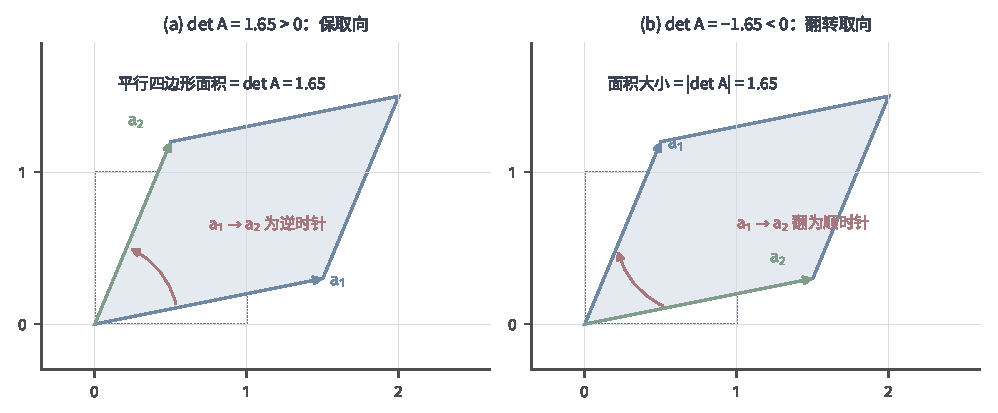
\includegraphics[width=169mm]{figures/01-mathematical-preliminaries-upper/03-linear-spaces/matplotlib/ls-determinant-oriented-volume/ls-determinant-oriented-volume.pdf}
  \caption{行列式作为有向体积的缩放。左：单位正方形由$\bm e_1=(1,0)$、$\bm e_2=(0,1)$张成，面积为$1$。中：$\bm A=\bigl(\begin{smallmatrix}2&0.5\\0&1.5\end{smallmatrix}\bigr)$把它映成由$\bm A\bm e_1=(2,0)$、$\bm A\bm e_2=(0.5,1.5)$张成的平行四边形，有向面积为$2\cdot1.5-0.5\cdot0=3=\det\bm A>0$（保定向）。右：$\bm A$把$\bm e_1$反射到$(-2,0)$，有向面积为$-3$（反定向）。向量与数值均为解析教学例。}
  \label{fig:ls-determinant-oriented-volume}
\end{figure*}

\paragraph{排列展开}
把$\bm A\bm e_j=\sum_i a_{i,j}\bm e_i$代入楔积并展开。若第$j$个因子选出$\bm e_{\tau(j)}$，得到的项为$\bigl(\prod_ja_{\tau(j),j}\bigr)\,\bm e_{\tau(1)}\wedge\cdots\wedge\bm e_{\tau(d)}$。下标有重复的项为零；留下的项中$\tau$是$\{1,\ldots,d\}$的一个排列，而$\bm e_{\tau(1)}\wedge\cdots\wedge\bm e_{\tau(d)}=\operatorname{sgn}(\tau)\,\bm e_1\wedge\cdots\wedge\bm e_d$。所以
\[
 \det\bm A=\sum_{\tau}\operatorname{sgn}(\tau)\prod_{j=1}^d a_{\tau(j),j},
\]
求和遍历全部排列。习惯上按行书写：记$\pi=\tau^{-1}$，把乘积按行号重排，得到$\prod_ia_{i,\pi(i)}$。$\tau$的逆序对$(i,j)$与$\pi$的逆序对$(\tau(j),\tau(i))$一一对应，所以$\operatorname{sgn}(\pi)=\operatorname{sgn}(\tau)$。于是得到计算公式
\[
 \det\bm A
 =\sum_{\pi\in S_d}\operatorname{sgn}(\pi)
   \prod_{i=1}^d a_{i,\pi(i)},
\]
其中$S_d$是$\{1,\ldots,d\}$到自身的全部双射，每个$\pi$规定第$i$行选取第$\pi(i)$列。计算步骤是：对每个排列，从每行各取一个元素、各列恰好取一次，把取出的$d$个数相乘，再按逆序对数的奇偶加上正负号求和。

二阶时只有两个排列：恒等排列没有逆序对，取正号；交换$1,2$的排列有一个逆序对，取负号。于是
\[
 \det\begin{pmatrix}a&b\\c&d\end{pmatrix}=ad-bc,
\]
例如$\det\left(\begin{smallmatrix}1&2\\3&4\end{smallmatrix}\right)=1\cdot4-2\cdot3=-2$。

三阶时有六个排列。恒等排列与两个循环排列$(\pi(1),\pi(2),\pi(3))=(2,3,1)$、$(3,1,2)$的逆序对数为$0$或$2$，取正号；只交换两个位置的三个排列$(1,3,2)$、$(2,1,3)$、$(3,2,1)$的逆序对数为$1$或$3$，取负号。于是
\[
 \begin{aligned}
 \det\bm A={}&a_{1,1}a_{2,2}a_{3,3}+a_{1,2}a_{2,3}a_{3,1}+a_{1,3}a_{2,1}a_{3,2}\\
 &-a_{1,1}a_{2,3}a_{3,2}-a_{1,2}a_{2,1}a_{3,3}-a_{1,3}a_{2,2}a_{3,1}.
 \end{aligned}
\]
下面用这个公式计算一个具体的三阶行列式。
\begin{example}[三阶行列式的排列展开]
\label{ex:ls-det-three-by-three}
给定：$\bm A=\left(\begin{smallmatrix}2&0&1\\1&3&0\\0&1&1\end{smallmatrix}\right)$。
计算：按上式的六项次序代入，
\[
 \begin{aligned}
 \det\bm A&=2\cdot3\cdot1+0\cdot0\cdot0+1\cdot1\cdot1-2\cdot0\cdot1-0\cdot1\cdot1-1\cdot3\cdot0\\
 &=6+0+1-0-0-0=7.
 \end{aligned}
\]
结论：$\det\bm A=7$。六项中只有两项非零，其余四项都含有零元素。
\end{example}

行列式因而是矩阵元素的多项式。上面的推导只说明：若楔积满足两条规则，行列式只能是这个和。反过来可以直接验证，排列展开式作为各列的函数确实对每列线性、交换两列时变号（交换两列相当于把每个$\pi$复合上一次对换，逆序对数的奇偶随之改变），并且在单位矩阵处等于$1$。所以两条规则彼此相容，行列式由它们和$\det\bm I_d=1$唯一确定。高阶时排列有$d!$个，实际计算改用下一小节的性质。

到这里，矩阵的运算都已定义。迹与行列式是方阵的两种不同的标量读取：同一个$\left(\begin{smallmatrix}1&2\\3&4\end{smallmatrix}\right)$迹为$5$而行列式为$-2$。下一小节逐一检查各运算满足的规则。

% 第4章第2节（下）：矩阵运算的性质，按运算分组（加法与数乘、转置、乘法、逐项乘积、逆、幂、迹、行列式、范数），每条性质先给结论再给证明或说明；常见矩阵（含正交矩阵）的性质分别放在相应运算之下。

\subsection{矩阵运算的性质}
\label{sec:ls-matrix-operation-properties}
\label{sec:prelim-matrix-operation-rules}
\label{sec:linear-algebra-map-composition}

上一小节只给出了各运算的算法；推导时还要知道哪些变形允许做。实数乘法的哪些规则保留下来，哪些不再成立？转置、求逆与乘法相遇时次序怎样变化？迹与行列式在乘法下怎样表现？矩阵范数怎样控制连续两次作用的放大？对角、三角、置换与正交矩阵在这些运算下又有哪些简单规律？本小节按运算分组回答，每条性质先写出结论，再给出证明或说明。以下凡写出乘积，都默认各因子的形状相容。

\subsubsection{加法与数乘的性质}

同形矩阵逐项相加与数乘，向量一节的八条规则在每个位置上照搬过来。对同形矩阵$\bm A,\bm B,\bm C$和实数$a,b$：
\[
\begin{aligned}
 &\bm A+\bm B=\bm B+\bm A, && (\bm A+\bm B)+\bm C=\bm A+(\bm B+\bm C),\\
 &\bm A+\bm0=\bm A, && \bm A+(-\bm A)=\bm0,\\
 &a(b\bm A)=(ab)\bm A, && 1\bm A=\bm A,\\
 &(a+b)\bm A=a\bm A+b\bm A, && a(\bm A+\bm B)=a\bm A+a\bm B.
\end{aligned}
\]
每一条都可以在任一位置$(i,j)$上用实数运算直接验证。

\subsubsection{转置的性质}
\label{sec:ls-reshaping}

\paragraph{与加法、数乘交换}
\[
 (\bm A+\bm B)^\top=\bm A^\top+\bm B^\top,\qquad
 (c\bm A)^\top=c\bm A^\top,\qquad
 (\bm A^\top)^\top=\bm A.
\]
转置只搬动元素，逐项运算的结果搬到新位置后不变；转置两次，每个元素回到原来的位置。

\paragraph{乘积的转置}
\[
 (\bm A\bm B)^\top=\bm B^\top\bm A^\top.
\]
乘积转置后因子次序反转。按元素公式，
\[
 \bigl((\bm A\bm B)^\top\bigr)_{i,j}=(\bm A\bm B)_{j,i}=\sum_\ell a_{j,\ell}b_{\ell,i}
 =\sum_\ell(\bm B^\top)_{i,\ell}(\bm A^\top)_{\ell,j}=(\bm B^\top\bm A^\top)_{i,j}.
\]
多个因子时依次使用，$(\bm A\bm B\bm C)^\top=\bm C^\top\bm B^\top\bm A^\top$。

\paragraph{内积中的转置}
\[
 \langle\bm A\bm x,\bm y\rangle=\langle\bm x,\bm A^\top\bm y\rangle,\qquad\bm A\in\mathbb R^{m\times d},\ \bm x\in\mathbb R^d,\ \bm y\in\mathbb R^m.
\]
由上一条，$(\bm A\bm x)^\top\bm y=\bm x^\top\bm A^\top\bm y$：在欧氏内积中，作用在左侧向量上的$\bm A$可以改写成作用在右侧向量上的$\bm A^\top$。

\paragraph{$\bm A^\top\bm A$对称}
对任意矩阵$\bm A$，$\bm A^\top\bm A$与$\bm A\bm A^\top$都是对称矩阵，因为$(\bm A^\top\bm A)^\top=\bm A^\top(\bm A^\top)^\top=\bm A^\top\bm A$，另一个同理。下面直接算出一个$\bm A\bm A^\top$。
\begin{example}[计算$\bm A\bm A^\top$]
\label{ex:ls-gram-product-symmetric}
给定：$\bm A=\left[\begin{smallmatrix}1&2&3\\4&5&6\end{smallmatrix}\right]$。
计算：$\bm A\bm A^\top$的$(i,j)$元是$\bm A$的第$i$行与第$j$行的内积，
\[
 \bm A\bm A^\top=\begin{bmatrix}1+4+9&4+10+18\\4+10+18&16+25+36\end{bmatrix}=\begin{bmatrix}14&32\\32&77\end{bmatrix}.
\]
结论：两个非对角元都是两行的内积$32$，结果是对称矩阵。
\end{example}

\paragraph{正交矩阵的转置条件}
$n$阶方阵$\bm Q$是正交矩阵，当且仅当
\[
 \bm Q^\top\bm Q=\bm I_n.
\]
$(\bm Q^\top\bm Q)_{i,j}$是$\bm Q$的第$i$列与第$j$列的内积。所以“各列都是单位向量”对应对角元等于$1$，“各列两两正交”对应非对角元等于$0$，两者合起来正是这个矩阵等式。下面用这个条件重新检验示例~\ref{ex:ls-rotation-orthogonal}中的两个矩阵。
\begin{example}[用转置条件检验正交矩阵]
\label{ex:ls-orthogonality-by-transpose}
给定：旋转矩阵$\bm R_\phi$与对角矩阵$\operatorname{diag}(2,1)$。
计算：
\[
 \begin{aligned}
 \bm R_\phi^\top\bm R_\phi
 &=\begin{bmatrix}\cos\phi&\sin\phi\\-\sin\phi&\cos\phi\end{bmatrix}
   \begin{bmatrix}\cos\phi&-\sin\phi\\\sin\phi&\cos\phi\end{bmatrix}\\
 &=\begin{bmatrix}\cos^2\phi+\sin^2\phi&0\\0&\sin^2\phi+\cos^2\phi\end{bmatrix}
 =\bm I_2,\\
 \operatorname{diag}(2,1)^\top\operatorname{diag}(2,1)&=\operatorname{diag}(4,1)\neq\bm I_2.
 \end{aligned}
\]
结论：$\bm R_\phi$满足转置条件，是正交矩阵；$\operatorname{diag}(2,1)$的乘积在$(1,1)$位置为$4\neq1$，对应第一列长度不为$1$。
\end{example}

\paragraph{正交矩阵保持内积}
\[
 \langle\bm Q\bm x,\bm Q\bm y\rangle=\langle\bm x,\bm y\rangle\qquad(\bm Q\text{为正交矩阵}).
\]
由内积中的转置与上一条，$\langle\bm Q\bm x,\bm Q\bm y\rangle=\langle\bm x,\bm Q^\top\bm Q\bm y\rangle=\langle\bm x,\bm y\rangle$。特别地，正交矩阵把两两正交的向量仍送到两两正交的向量。

\subsubsection{乘法的性质}

\paragraph{单位乘}
\[
 \bm I_m\bm A=\bm A=\bm A\bm I_d,\qquad\bm A\in\mathbb R^{m\times d}.
\]
$\bm I_m$的第$i$行是$\bm e_i^\top$，它与$\bm A$的第$j$列相乘取出$a_{i,j}$；右乘同理。单位矩阵在矩阵乘法中的作用相当于数$1$在实数乘法中的作用。

\paragraph{零乘}
\[
 \bm0\bm A=\bm0,\qquad\bm A\bm0=\bm0.
\]
乘积的每个元素都是若干乘积之和，其中一个因子全为零时，每一项都为零。这里各个零矩阵的形状由相乘的另一个因子决定。

反过来不成立：$\bm A\bm B=\bm0$不能推出$\bm A=\bm0$或$\bm B=\bm0$，下面是一个反例。
\begin{example}[反例：两个非零矩阵的乘积为零]
\label{ex:ls-zero-product-nonzero-factors}
给定：$\bm A=\left[\begin{smallmatrix}1&0\\0&0\end{smallmatrix}\right]$，$\bm B=\left[\begin{smallmatrix}0&0\\1&0\end{smallmatrix}\right]$，两者都不是零矩阵。
计算：
\[
 \bm A\bm B=\begin{bmatrix}1\cdot0+0\cdot1&1\cdot0+0\cdot0\\0\cdot0+0\cdot1&0\cdot0+0\cdot0\end{bmatrix}=\begin{bmatrix}0&0\\0&0\end{bmatrix}.
\]
结论：$\bm A\bm B=\bm0$，而$\bm A\neq\bm0$、$\bm B\neq\bm0$。
\end{example}
原因可以按列看出。由乘积的元素公式，$\bm A\bm B$的第$j$列就是$\bm A$乘$\bm B$的第$j$列，所以$\bm A\bm B=\bm0$恰好意味着$\bm B$的每一列$\bm b$都满足$\bm A\bm b=\bm0$：右因子产生的结果被左因子完全消去。上例中$\bm A$只保留第一个坐标、把第二个坐标清零，而$\bm B$的第一列$(0,1)^\top$只有第二个坐标非零，第二列为零。

\paragraph{结合律}
\[
 (\bm A\bm B)\bm C=\bm A(\bm B\bm C).
\]
按式~\eqref{eq:prelim-matrix-composition}展开，两边的第$(i,j)$项都是$\sum_k\sum_l a_{i,k}b_{k,l}c_{l,j}$，只是两个有限求和的次序不同。这也是函数复合满足结合律（第~\ref{sec:prelim-map-operations}节）在矩阵上的翻译。由结合律，多个相容矩阵连乘时不必标出括号。

\paragraph{分配律与数乘相容}
\[
 \bm A(\bm B+\bm C)=\bm A\bm B+\bm A\bm C,\qquad
 (\bm A+\bm B)\bm C=\bm A\bm C+\bm B\bm C,\qquad
 c(\bm A\bm B)=(c\bm A)\bm B=\bm A(c\bm B),
\]
逐项展开有限和即得。把右因子取为列向量，得到矩阵与向量的乘积对输入保持线性组合：
\begin{equation}
 \bm A(a\bm u+b\bm v)=a\bm A\bm u+b\bm A\bm v,
 \qquad\bm u,\bm v\in\mathbb R^d,\quad a,b\in\mathbb R.
 \label{eq:prelim-matrix-linearity}
\end{equation}

由这一性质，函数$\bm u\mapsto\bm A\bm u$由它在$\bm e_1,\ldots,\bm e_d$上的输出完全确定：因为$\bm u=\sum_ju_j\bm e_j$，所以$\bm A\bm u=\sum_ju_j\bm A\bm e_j$，而这些输出$\bm A\bm e_j$就是$\bm A$的各列。第~\ref{chap:linear-representation}章把保持线性组合的函数称为线性映射，并说明每个这样的映射都能由一张矩阵记录。

\paragraph{分块乘法}
把矩阵按行、列分成尺寸相容的块，乘法规则对块照样成立：
\[
 \begin{bmatrix}\bm A&\bm B\end{bmatrix}\begin{bmatrix}\bm C\\\bm D\end{bmatrix}=\bm A\bm C+\bm B\bm D,
 \qquad
 \begin{bmatrix}\bm A\\\bm B\end{bmatrix}\bm C=\begin{bmatrix}\bm A\bm C\\\bm B\bm C\end{bmatrix},
\]
\[
 \bm A\begin{bmatrix}\bm C&\bm D\end{bmatrix}=\begin{bmatrix}\bm A\bm C&\bm A\bm D\end{bmatrix},
\]
以及$2\times2$分块的乘积
\[
 \begin{bmatrix}\bm A_{1,1}&\bm A_{1,2}\\\bm A_{2,1}&\bm A_{2,2}\end{bmatrix}
 \begin{bmatrix}\bm B_{1,1}&\bm B_{1,2}\\\bm B_{2,1}&\bm B_{2,2}\end{bmatrix}
 =\begin{bmatrix}
  \bm A_{1,1}\bm B_{1,1}+\bm A_{1,2}\bm B_{2,1}&\bm A_{1,1}\bm B_{1,2}+\bm A_{1,2}\bm B_{2,2}\\
  \bm A_{2,1}\bm B_{1,1}+\bm A_{2,2}\bm B_{2,1}&\bm A_{2,1}\bm B_{1,2}+\bm A_{2,2}\bm B_{2,2}
 \end{bmatrix}.
\]
条件是每个相乘的块对中，左块的列数等于右块的行数。第一式成立，是因为式~\eqref{eq:prelim-matrix-composition}对中间索引$\ell$的求和可以分段进行：前一段$\ell$对应$\bm A$的列与$\bm C$的行，后一段对应$\bm B$的列与$\bm D$的行，两段之和逐项等于整段求和。后两式只是把结果的行或列分组，$2\times2$分块由这三式合成。块可以像数一样参与运算，只是块之间的次序不能交换。

把块分到最细，得到三种常用的特例。右因子按列分块，得$(\bm A\bm B)_{:,j}=\bm A\bm B_{:,j}$：$\bm A$分别乘$\bm B$的每一列。左因子按行分块，得$(\bm A\bm B)_{i,:}=\bm A_{i,:}\bm B$：结果的第$i$行是$\bm B$各行以$\bm A_{i,:}$的元素为系数的线性组合。

第三种特例把中间维数$d$分成长度为$1$的$d$段，这时第一式给出
\begin{equation}
 \bm A\bm B=\sum_{\ell=1}^d\bm A_{:,\ell}\bm B_{\ell,:},
 \label{eq:ls-product-outer-sum}
\end{equation}
其中一列$\bm A_{:,\ell}\in\mathbb R^{m\times1}$乘一行$\bm B_{\ell,:}\in\mathbb R^{1\times k}$，得到$(i,j)$元素为$a_{i,\ell}b_{\ell,j}$的$m\times k$矩阵。式~\eqref{eq:ls-product-outer-sum}是后面低秩近似的出发点。下面用示例~\ref{ex:ls-matrix-product-2x2}的乘积核对这个公式。
\begin{example}[把乘积写成列乘行之和]
\label{ex:ls-product-as-outer-sum}
给定：示例~\ref{ex:ls-matrix-product-2x2}中的$\bm A=\left(\begin{smallmatrix}1&1\\0&1\end{smallmatrix}\right)$与$\bm B=\left(\begin{smallmatrix}1&0\\0&2\end{smallmatrix}\right)$。
计算：$\bm A$的两列为$(1,0)^\top$与$(1,1)^\top$，$\bm B$的两行为$(1,0)$与$(0,2)$，
\[
 \bm A\bm B=\begin{pmatrix}1\\0\end{pmatrix}\begin{pmatrix}1&0\end{pmatrix}+\begin{pmatrix}1\\1\end{pmatrix}\begin{pmatrix}0&2\end{pmatrix}
 =\begin{pmatrix}1&0\\0&0\end{pmatrix}+\begin{pmatrix}0&2\\0&2\end{pmatrix}=\begin{pmatrix}1&2\\0&2\end{pmatrix}.
\]
结论：两个“列乘行”矩阵之和与逐项计算的乘积相同。
\end{example}

\paragraph{交换律不成立}
一般$\bm A\bm B\neq\bm B\bm A$。形状不同时，两个乘积甚至不一定都有定义；即使两个因子是同阶方阵，两种次序的乘积也可能不同，下面是一个反例。
\begin{example}[反例：先交换再保留与先保留再交换]
\label{ex:ls-noncommuting-pair}
给定：只保留第一个坐标的$\bm P=\left[\begin{smallmatrix}1&0\\0&0\end{smallmatrix}\right]$，交换两个坐标的$\bm S=\left[\begin{smallmatrix}0&1\\1&0\end{smallmatrix}\right]$。
计算：
\[
 \bm P\bm S=\begin{bmatrix}0&1\\0&0\end{bmatrix},\qquad
 \bm S\bm P=\begin{bmatrix}0&0\\1&0\end{bmatrix}.
\]
结论：$\bm P\bm S\neq\bm S\bm P$。作用在$\bm u\in\mathbb R^2$上，$\bm P\bm S\bm u=(u_2,0)^\top$是先交换、再保留第一个坐标，$\bm S\bm P\bm u=(0,u_1)^\top$是先保留、再交换，两种次序的结果不同。
\end{example}
书写$\bm A\bm B\bm x$时，作用顺序是从右向左：先$\bm B$，后$\bm A$。

\paragraph{消去律不成立}
$\bm A\bm B=\bm A\bm C$且$\bm A\neq\bm0$不能推出$\bm B=\bm C$。原因是$\bm A\bm B=\bm A\bm C$等价于$\bm A(\bm B-\bm C)=\bm0$，而乘积为零不能推出$\bm B-\bm C=\bm0$。下面用示例~\ref{ex:ls-zero-product-nonzero-factors}构造反例。
\begin{example}[反例：非零的左因子不能消去]
\label{ex:ls-cancellation-fails}
给定：示例~\ref{ex:ls-zero-product-nonzero-factors}中的$\bm A=\left[\begin{smallmatrix}1&0\\0&0\end{smallmatrix}\right]$与$\bm B=\left[\begin{smallmatrix}0&0\\1&0\end{smallmatrix}\right]$，以及$\bm C=\bm0$。
验证：$\bm A\bm B=\bm0=\bm A\bm C$，而$\bm B\neq\bm C$。
结论：虽然$\bm A\bm B=\bm A\bm C$且$\bm A\neq\bm0$，却不能消去$\bm A$得到$\bm B=\bm C$。
\end{example}
若$\bm A$是可逆方阵，在$\bm A\bm B=\bm A\bm C$两边左乘$\bm A^{-1}$即得$\bm B=\bm C$。所以左因子可逆时可以消去，一般的非零因子则不能。

常见矩阵参与乘法时，结果有固定模式。下面逐类给出。

\paragraph{对角矩阵的乘法}
对$\bm D=\operatorname{diag}(d_1,\ldots,d_n)$，
\[
 (\bm D\bm A)_{i,j}=d_i\bm A_{i,j},\qquad(\bm A\bm D)_{i,j}=\bm A_{i,j}d_j,
\]
\[
 \operatorname{diag}(d_1,\ldots,d_n)\operatorname{diag}(e_1,\ldots,e_n)=\operatorname{diag}(d_1e_1,\ldots,d_ne_n).
\]
左乘对角矩阵缩放各行，右乘缩放各列：乘积公式中只有$\ell=i$（左乘时）或$\ell=j$（右乘时）的一项留下。作用在向量上，$\bm D\bm u=(d_1u_1,\ldots,d_nu_n)^\top$是逐坐标缩放。两个对角矩阵相乘时对角元逐个相乘，所以对角矩阵之间可以交换次序。下面的例子比较左乘与右乘。
\begin{example}[左乘与右乘对角矩阵]
\label{ex:ls-diagonal-scaling}
给定：$\bm D=\operatorname{diag}(2,3)$，$\bm A=\left[\begin{smallmatrix}1&2\\3&4\end{smallmatrix}\right]$。
计算：
\[
 \begin{aligned}
 \bm D\bm A&=\begin{bmatrix}2\cdot1&2\cdot2\\3\cdot3&3\cdot4\end{bmatrix}=\begin{bmatrix}2&4\\9&12\end{bmatrix},\\
 \bm A\bm D&=\begin{bmatrix}1\cdot2&2\cdot3\\3\cdot2&4\cdot3\end{bmatrix}=\begin{bmatrix}2&6\\6&12\end{bmatrix}.
 \end{aligned}
\]
结论：左乘把第一、二行分别乘以$2$、$3$，右乘把第一、二列分别乘以$2$、$3$。两个结果不同，所以对角矩阵与一般矩阵相乘时仍要区分左右。
\end{example}

\paragraph{三角矩阵的乘法}
若$\bm A,\bm B$都是$n$阶上三角矩阵，则$\bm A\bm B$也是上三角矩阵，并且
\[
 (\bm A\bm B)_{i,i}=\bm A_{i,i}\bm B_{i,i}.
\]
在$(\bm A\bm B)_{i,j}=\sum_\ell\bm A_{i,\ell}\bm B_{\ell,j}$中，$\bm A_{i,\ell}$只在$\ell\geq i$时可能非零，$\bm B_{\ell,j}$只在$\ell\leq j$时可能非零，所以只有$i\leq\ell\leq j$的项可能非零：$i>j$时没有这样的$\ell$，乘积元素为零；$i=j$时只剩$\ell=i$一项。下三角矩阵同理：两个下三角矩阵的乘积仍是下三角矩阵，对角元逐个相乘。下面是一个二阶算例。
\begin{example}[两个上三角矩阵的乘积]
\label{ex:ls-upper-triangular-product}
给定：$\bm A=\left[\begin{smallmatrix}1&2\\0&3\end{smallmatrix}\right]$，$\bm B=\left[\begin{smallmatrix}4&5\\0&6\end{smallmatrix}\right]$。
计算：
\[
 \bm A\bm B=\begin{bmatrix}1\cdot4+2\cdot0&1\cdot5+2\cdot6\\0\cdot4+3\cdot0&0\cdot5+3\cdot6\end{bmatrix}=\begin{bmatrix}4&17\\0&18\end{bmatrix}.
\]
结论：乘积仍是上三角矩阵，对角元$4=1\cdot4$、$18=3\cdot6$是两个因子对角元的乘积；右上角的$17$则同时用到了两个因子的非对角元。
\end{example}

\paragraph{置换矩阵的乘法}
设$\bm P=\left[\begin{smallmatrix}\bm e_{\sigma(1)}&\cdots&\bm e_{\sigma(n)}\end{smallmatrix}\right]$，其中$\sigma$是$\{1,\ldots,n\}$上的排列，则
\[
 (\bm P\bm A)_{\sigma(i),:}=\bm A_{i,:},\qquad(\bm A\bm P)_{:,j}=\bm A_{:,\sigma(j)}.
\]
即左乘把$\bm A$的第$i$行移到第$\sigma(i)$行，右乘使$\bm A\bm P$的第$j$列取自$\bm A$的第$\sigma(j)$列。例如$\left[\begin{smallmatrix}0&1\\1&0\end{smallmatrix}\right]$左乘交换两行、右乘交换两列。两个置换矩阵的乘积仍是置换矩阵：设$\bm P'$是另一个置换矩阵，$\bm P'\bm P$的第$j$列是$\bm P'\bm e_{\sigma(j)}$，即$\bm P'$的第$\sigma(j)$列；它是标准坐标向量，而且不同的$j$取到$\bm P'$的不同列，所以这些列互不相同。

\paragraph{正交矩阵的乘法}
若$\bm Q_1,\bm Q_2$是$n$阶正交矩阵，则
\[
 (\bm Q_1\bm Q_2)^\top(\bm Q_1\bm Q_2)=\bm Q_2^\top\bm Q_1^\top\bm Q_1\bm Q_2=\bm Q_2^\top\bm Q_2=\bm I_n,
\]
由正交矩阵的转置条件，$\bm Q_1\bm Q_2$仍是正交矩阵。下面的例子显示，两个平面旋转的乘积不仅是正交矩阵，而且仍是旋转。
\begin{example}[两个平面旋转的乘积]
\label{ex:ls-rotation-composition}
给定：旋转矩阵$\bm R_\phi$与$\bm R_\psi$。
计算：直接相乘，再用和角公式$\cos(\phi+\psi)=\cos\phi\cos\psi-\sin\phi\sin\psi$与$\sin(\phi+\psi)=\sin\phi\cos\psi+\cos\phi\sin\psi$，
\[
 \begin{aligned}
 \bm R_\phi\bm R_\psi
 &=\begin{bmatrix}\cos\phi\cos\psi-\sin\phi\sin\psi&-\cos\phi\sin\psi-\sin\phi\cos\psi\\\sin\phi\cos\psi+\cos\phi\sin\psi&-\sin\phi\sin\psi+\cos\phi\cos\psi\end{bmatrix}\\
 &=\bm R_{\phi+\psi}.
 \end{aligned}
\]
结论：先转$\psi$角、再转$\phi$角，等于一次转$\phi+\psi$角；乘积是正交矩阵，与上面的一般结论一致。
\end{example}

\paragraph{对称矩阵的乘积}
若$\bm A,\bm B$是同阶对称矩阵，则
\[
 (\bm A\bm B)^\top=\bm B^\top\bm A^\top=\bm B\bm A,
\]
所以$\bm A\bm B$对称当且仅当$\bm A\bm B=\bm B\bm A$。对称矩阵的乘积一般不对称，下面是一个反例。
\begin{example}[反例：两个对称矩阵的乘积不对称]
\label{ex:ls-symmetric-product-not-symmetric}
给定：对称矩阵$\bm A=\left[\begin{smallmatrix}1&1\\1&0\end{smallmatrix}\right]$与$\bm B=\operatorname{diag}(1,2)$。
计算：右乘对角矩阵缩放各列，
\[
 \bm A\bm B=\begin{bmatrix}1\cdot1&1\cdot2\\1\cdot1&0\cdot2\end{bmatrix}=\begin{bmatrix}1&2\\1&0\end{bmatrix}.
\]
结论：$(\bm A\bm B)_{1,2}=2\neq1=(\bm A\bm B)_{2,1}$，乘积不对称。这与上面的判据一致：$\bm B\bm A=\left[\begin{smallmatrix}1&1\\2&0\end{smallmatrix}\right]\neq\bm A\bm B$。
\end{example}

\subsubsection{逐项乘积的性质}

\paragraph{交换律}
\[
 \bm A\odot\bm B=\bm B\odot\bm A.
\]
式~\eqref{eq:ls-hadamard}右端只是实数乘法，按位置逐项验证即得。逐项乘积可交换而矩阵乘积不可交换，再次说明两者是不同的运算。

\paragraph{结合律}
\[
 (\bm A\odot\bm B)\odot\bm C=\bm A\odot(\bm B\odot\bm C),
\]
两边的$(i,j)$元素都是$a_{i,j}b_{i,j}c_{i,j}$。

\paragraph{分配律}
\[
 \bm A\odot(\bm B+\bm C)=\bm A\odot\bm B+\bm A\odot\bm C,
\]
两边的$(i,j)$元素都是$a_{i,j}(b_{i,j}+c_{i,j})$。

\paragraph{单位元是全$1$数组}
全部元素为$1$的同形数组$\bm J$满足$\bm J\odot\bm A=\bm A$。单位矩阵不是逐项乘积的单位元：$\bm I_2\odot\bm A$只保留$\bm A$的对角元，把非对角元都变为零。

\paragraph{对每个因子分别线性}
固定一个因子时，$\bm X\mapsto\bm M\odot\bm X$保持线性组合。两个因子都作为未知量时，乘积只对各自分别线性：同时把两者放大两倍，结果放大四倍。第~\ref{chap:linear-representation}章换一组记录方向以后会看到，矩阵乘积对应的复合关系保持不变，逐项乘积则随记录方式改变。

\subsubsection{逆的性质}

设下面的$\bm A,\bm B$都是$n$阶可逆方阵。

\paragraph{乘积的逆}
\begin{equation}
 (\bm A\bm B)^{-1}=\bm B^{-1}\bm A^{-1}.
 \label{eq:ls-inverse-product}
\end{equation}
先作用的后撤销，就像先穿袜子再穿鞋，脱的时候要先脱鞋。验证：$(\bm A\bm B)(\bm B^{-1}\bm A^{-1})=\bm A(\bm B\bm B^{-1})\bm A^{-1}=\bm A\bm A^{-1}=\bm I_n$，反方向$(\bm B^{-1}\bm A^{-1})(\bm A\bm B)=\bm I_n$同理。

\paragraph{逆的逆}
\[
 (\bm A^{-1})^{-1}=\bm A.
\]
定义中$\bm A$与$\bm A^{-1}$的地位对称：$\bm A^{-1}\bm A=\bm A\bm A^{-1}=\bm I_n$同样说明$\bm A$是$\bm A^{-1}$的逆。

\paragraph{数乘的逆}
\[
 (c\bm A)^{-1}=c^{-1}\bm A^{-1}\qquad(c\neq0).
\]
直接相乘：$(c\bm A)(c^{-1}\bm A^{-1})=(cc^{-1})\bm A\bm A^{-1}=\bm I_n$，反方向同理。

\paragraph{转置的逆}
\[
 (\bm A^\top)^{-1}=(\bm A^{-1})^\top.
\]
由乘积的转置，$\bm A^\top(\bm A^{-1})^\top=(\bm A^{-1}\bm A)^\top=\bm I^\top=\bm I$，反方向同理，所以$(\bm A^{-1})^\top$就是$\bm A^\top$的逆。

\paragraph{正交矩阵的逆}
\[
 \bm Q^{-1}=\bm Q^\top,\qquad\bm Q\bm Q^\top=\bm I_n\qquad(\bm Q\text{为正交矩阵}).
\]
正交矩阵的转置条件$\bm Q^\top\bm Q=\bm I_n$只说明$\bm Q^\top$是$\bm Q$的左逆。方阵只要有一侧的逆就可逆，而且这个单侧逆就是逆矩阵；这一点的证明要用到行列式，放在第~\ref{sec:ls-square-one-sided-inverse}节。由此$\bm Q^{-1}=\bm Q^\top$，另一侧的乘积$\bm Q\bm Q^\top$也等于$\bm I_n$。

$\bm Q\bm Q^\top$的$(i,j)$元是$\bm Q$的第$i$行与第$j$行的内积，所以正交矩阵的各行同样两两正交且长度为$1$，求逆只需转置。又因$(\bm Q^\top)^\top\bm Q^\top=\bm Q\bm Q^\top=\bm I_n$，由转置条件，$\bm Q^{-1}=\bm Q^\top$也是正交矩阵。

\subsubsection{幂的性质}

设$\bm A$为方阵，$m,n$为非负整数；$\bm A$可逆时，$m,n$可取任意整数。

\paragraph{同底幂相乘}
\[
 \bm A^m\bm A^n=\bm A^{m+n}.
\]
由结合律，两边都是同样个数的$\bm A$（或$\bm A^{-1}$）连乘；指数异号时，相邻的$\bm A\bm A^{-1}$逐对消去。交换$m,n$的角色可见，同一矩阵的不同次幂彼此可以交换。

\paragraph{幂的幂}
\[
 (\bm A^m)^n=\bm A^{mn}.
\]
左边是$n$组、每组$m$个因子的连乘，由结合律去掉括号即得。

\paragraph{负幂与逆相容}
\[
 (\bm A^k)^{-1}=(\bm A^{-1})^k=\bm A^{-k}.
\]
对$k$个相同因子反复使用式~\eqref{eq:ls-inverse-product}即得。

\subsubsection{迹的性质}
\phantomsection
\label{sec:ls-matrix-contractions}

\paragraph{线性}
\[
 \operatorname{tr}(a\bm A+b\bm B)=a\operatorname{tr}(\bm A)+b\operatorname{tr}(\bm B),
\]
这是有限和的线性。

\paragraph{转置不变}
\[
 \operatorname{tr}(\bm A^\top)=\operatorname{tr}(\bm A),
\]
因为转置不改变对角元。

\paragraph{循环性}
对$\bm A\in\mathbb R^{m\times n}$、$\bm B\in\mathbb R^{n\times m}$，
\begin{equation}
 \operatorname{tr}(\bm A\bm B)
 =\sum_{i=1}^m\sum_{j=1}^n A_{i,j}B_{j,i}
 =\operatorname{tr}(\bm B\bm A).
 \label{eq:linear-algebra-trace-cyclic}
\end{equation}
两个双重和只是求和次序不同。$\bm A\bm B$与$\bm B\bm A$可以是不同阶的方阵，相等的是迹，不是矩阵本身，下面的例子说明这一点。
\begin{example}[不同阶乘积的迹相等]
\label{ex:ls-trace-cyclic-different-sizes}
给定：$\bm A=\left[\begin{smallmatrix}1&2&3\end{smallmatrix}\right]\in\mathbb R^{1\times3}$，$\bm B=(1,0,2)^\top\in\mathbb R^{3\times1}$。
计算：$\bm A\bm B=1\cdot1+2\cdot0+3\cdot2=7$是$1\times1$矩阵；
\[
 \bm B\bm A=\begin{bmatrix}1&2&3\\0&0&0\\2&4&6\end{bmatrix}
\]
是$3\times3$矩阵，对角元为$1,0,6$。
结论：$\operatorname{tr}(\bm A\bm B)=7=1+0+6=\operatorname{tr}(\bm B\bm A)$，而两个乘积的阶数不同。
\end{example}

三个因子时，循环性只允许把因子整体循环移动：
\[
 \operatorname{tr}(\bm A\bm B\bm C)=\operatorname{tr}(\bm B\bm C\bm A)=\operatorname{tr}(\bm C\bm A\bm B).
\]
第一个等号把$\bm A$与$\bm B\bm C$看作两个因子使用式~\eqref{eq:linear-algebra-trace-cyclic}，第二个等号把$\bm A\bm B$与$\bm C$看作两个因子。任意交换相邻因子则可能改变迹，下面是一个反例。
\begin{example}[反例：交换相邻因子会改变迹]
\label{ex:ls-trace-adjacent-swap}
给定：$\bm A=\left(\begin{smallmatrix}1&0\\0&0\end{smallmatrix}\right)$，$\bm B=\left(\begin{smallmatrix}0&0\\1&0\end{smallmatrix}\right)$，$\bm C=\left(\begin{smallmatrix}0&1\\0&0\end{smallmatrix}\right)$。
计算：$\bm A\bm B=\bm0$，所以$\bm A\bm B\bm C=\bm0$。另一方面$\bm A\bm C=\bm C$，所以
\[
 \bm A\bm C\bm B=\begin{pmatrix}0&1\\0&0\end{pmatrix}\begin{pmatrix}0&0\\1&0\end{pmatrix}=\begin{pmatrix}1&0\\0&0\end{pmatrix}.
\]
结论：$\operatorname{tr}(\bm A\bm B\bm C)=0$，而$\operatorname{tr}(\bm A\bm C\bm B)=1$；交换$\bm B$与$\bm C$的次序改变了迹。
\end{example}

\paragraph{Frobenius内积的迹表示}
\[
 \langle\bm A,\bm B\rangle_{\mathrm F}=\operatorname{tr}(\bm A^\top\bm B),\qquad
 \lVert\bm A\rVert_{\mathrm F}^2=\operatorname{tr}(\bm A^\top\bm A).
\]
$\bm A^\top\bm B$的第$j$个对角元为$\sum_i A_{i,j}B_{i,j}$，再对$j$求和恰好遍历所有位置。反过来，计算$\operatorname{tr}(\bm A\bm B)$时也不必形成乘积：只需算$\sum_{i,j}A_{i,j}B_{j,i}$，代价为$mn$次乘法，而形成整个$\bm A\bm B$需要$m^2n$次。

\subsubsection{行列式的性质}
\label{sec:ls-determinant-properties}
\phantomsection
\label{sec:prelim-determinants}

行列式由楔积的两条规则定义，下面前两条性质就是这两条规则在列上的表述，其余性质由它们推出。设$\bm A,\bm B$为$d$阶方阵。

\paragraph{对列的多线性}
\[
 \det\begin{bmatrix}\cdots&a\bm u+b\bm w&\cdots\end{bmatrix}
 =a\det\begin{bmatrix}\cdots&\bm u&\cdots\end{bmatrix}
 +b\det\begin{bmatrix}\cdots&\bm w&\cdots\end{bmatrix},
\]
其中三个矩阵只在同一列不同，其余各列相同。$\det\bm A$是各列楔积的系数，所以这正是楔积对每个因子保持线性组合的直接翻译。

\paragraph{交替性}
交换两列，行列式变号；两列相同，行列式为零。前者来自楔积交换两个因子时变号（不相邻的两个因子可以经奇数次相邻交换互换位置）；后者是因为交换两个相同的列不改变矩阵，行列式却要变号，只能为零。

两条合起来又得到两个常用推论。把某列的倍数加到另一列上，行列式不变：按多线性拆开，多出的一项含两列相同，为零。某一列是其余各列的线性组合时，行列式为零：把这一列按组合展开，每一项都含两列相同。例如$\det\left(\begin{smallmatrix}1&2\\2&4\end{smallmatrix}\right)=4-4=0$，第二列是第一列的$2$倍。

\paragraph{转置不变}
\[
 \det(\bm A^\top)=\det\bm A.
\]
在排列展开中，把每一项的乘积按列号重排，得$\prod_ia_{i,\pi(i)}=\prod_ja_{\pi^{-1}(j),j}$；排列展开的推导已经说明$\operatorname{sgn}(\pi^{-1})=\operatorname{sgn}(\pi)$。$\pi$遍历$S_d$时，$\sigma=\pi^{-1}$也遍历$S_d$，所以
\[
 \det\bm A=\sum_{\sigma\in S_d}\operatorname{sgn}(\sigma)\prod_{j=1}^da_{\sigma(j),j}
 =\sum_{\sigma\in S_d}\operatorname{sgn}(\sigma)\prod_{j=1}^d(\bm A^\top)_{j,\sigma(j)}
 =\det(\bm A^\top).
\]
于是对列成立的多线性与交替性，对行同样成立。

\paragraph{数乘与加法}
\[
 \det(c\bm A)=c^d\det\bm A,\qquad
 \det(\bm A+\bm B)\neq\det\bm A+\det\bm B\ (\text{一般}).
\]
数乘把$d$列各乘以$c$，由对每列的线性提出$d$个$c$。行列式只对每一列分别线性，对整个矩阵却不是线性的，下面是一个反例。
\begin{example}[反例：行列式不保持加法]
\label{ex:ls-det-not-additive}
给定：$\bm A=\bm B=\bm I_2$。
计算：$\det\bm A+\det\bm B=1+1=2$，而由第一式，$\det(\bm A+\bm B)=\det(2\bm I_2)=2^2\det\bm I_2=4$。
结论：$\det(\bm A+\bm B)\neq\det\bm A+\det\bm B$。
\end{example}

\paragraph{乘法性}
\[
 \det(\bm A\bm B)=\det\bm A\,\det\bm B.
\]
接连作用两次时，体积缩放倍数应当相乘。排列展开的推导只用到楔积的两条规则，所以把$\bm e_1,\ldots,\bm e_d$换成任意向量$\bm w_1,\ldots,\bm w_d$，同样有$\bigwedge_j\bigl(\sum_ib_{i,j}\bm w_i\bigr)=(\det\bm B)\,\bm w_1\wedge\cdots\wedge\bm w_d$。由$(\bm A\bm B)\bm e_j=\bm A(\bm B\bm e_j)=\sum_i b_{i,j}\bm A\bm e_i$，取$\bm w_i=\bm A\bm e_i$，得到
\[
 (\bm A\bm B)\bm e_1\wedge\cdots\wedge(\bm A\bm B)\bm e_d
 =(\det\bm B)\,\bm A\bm e_1\wedge\cdots\wedge\bm A\bm e_d
 =(\det\bm A)(\det\bm B)\,\bm e_1\wedge\cdots\wedge\bm e_d.
\]
尽管矩阵乘法不可交换，$\det(\bm A\bm B)=\det(\bm B\bm A)$总成立，因为两边都等于$\det\bm A\,\det\bm B$。

\paragraph{三角矩阵的行列式}
\[
 \det\bm A=a_{1,1}a_{2,2}\cdots a_{d,d}\qquad(\bm A\text{为上三角或下三角矩阵}).
\]
设$\bm A$为上三角矩阵。排列$\pi$不是恒等排列时，必有某行$i$满足$\pi(i)<i$（因为$\sum_i(\pi(i)-i)=0$而各项不全为零），这一行选到主对角线下方的零元素，所以这一项为零；排列展开中只剩恒等排列一项。下三角时同理。例如$\det\left(\begin{smallmatrix}1&2&3\\0&4&5\\0&0&6\end{smallmatrix}\right)=1\cdot4\cdot6=24$；特别地，$\det\operatorname{diag}(d_1,\ldots,d_d)=d_1\cdots d_d$，$\det\bm I=1$。与乘法性合起来，两个上三角矩阵乘积的行列式就是两者全部对角元之积，这与三角矩阵乘积的对角元逐个相乘一致。

\paragraph{按行（列）展开}
对$d\geq2$，删除第$i$行、第$j$列得到的$(d-1)$阶子矩阵记为$\bm A^{(i,j)}$，定义\term{代数余子式}（cofactor）
\[
 C_{i,j}=(-1)^{i+j}\det\bm A^{(i,j)}.
\]
则对任一行$i$与任一列$j$，
\[
 \det\bm A=\sum_{j=1}^d a_{i,j}C_{i,j}=\sum_{i=1}^d a_{i,j}C_{i,j}.
\]
把排列展开按第$i$行选取的列分类，选第$j$列的各项之和正是$a_{i,j}C_{i,j}$；按列同理。下面沿第一行展开示例~\ref{ex:ls-det-three-by-three}中的矩阵，与排列展开的结果对照。
\begin{example}[沿第一行展开三阶行列式]
\label{ex:ls-det-cofactor-expansion}
给定：$\bm A=\left(\begin{smallmatrix}2&0&1\\1&3&0\\0&1&1\end{smallmatrix}\right)$。
计算：第一行元素为$2,0,1$，对应代数余子式的符号依次为$+,-,+$，
\[
 \begin{aligned}
 \det\bm A
 &=2\cdot\det\begin{pmatrix}3&0\\1&1\end{pmatrix}
 -0\cdot\det\begin{pmatrix}1&0\\0&1\end{pmatrix}
 +1\cdot\det\begin{pmatrix}1&3\\0&1\end{pmatrix}\\
 &=2\cdot3-0\cdot1+1\cdot1=7.
 \end{aligned}
\]
结论：结果与示例~\ref{ex:ls-det-three-by-three}的排列展开一致。
\end{example}

\paragraph{古典伴随恒等式}
把全部代数余子式排成矩阵$\bm C$，其转置称为\term{古典伴随}（classical adjugate）$\operatorname{adj}(\bm A)=\bm C^\top$。
\begin{theorem}[古典伴随恒等式]
\label{thm:ls-adjugate-identity}
对任意$d$阶方阵$\bm A$，
\[
 \bm A\,\operatorname{adj}(\bm A)
 =\operatorname{adj}(\bm A)\,\bm A
 =(\det\bm A)\,\bm I_d.
\]
\end{theorem}
\begin{proof}
乘积$\bm A\bm C^\top$的$(i,k)$元素为$\sum_j a_{i,j}C_{k,j}$。当$i=k$时，这正是沿第$i$行展开的$\det\bm A$。当$i\neq k$时，$C_{k,j}$不涉及第$k$行的元素，所以这个和是把第$k$行换成第$i$行后的矩阵沿第$k$行的展开；新矩阵有两行相同，行列式为零。于是$\bm A\bm C^\top=(\det\bm A)\bm I_d$。按列展开同样得到$\bm C^\top\bm A=(\det\bm A)\bm I_d$。
\end{proof}
二阶时$\operatorname{adj}\left(\begin{smallmatrix}a&b\\c&d\end{smallmatrix}\right)=\left(\begin{smallmatrix}d&-b\\-c&a\end{smallmatrix}\right)$，恒等式两边除以$ad-bc$就是上一小节的二阶求逆公式。

古典伴随是由余子式得到的代数构造，与第~\ref{chap:linear-representation}章由内积配对定义的伴随不是同一个对象。高阶时展开余子式的代价是阶乘级的，所以恒等式主要作为证明工具：下面用它证明方阵的单侧逆即逆，第~\ref{sec:ls-determinant-invertibility}节用它给出可逆判据，第~\ref{sec:ls-characteristic-polynomial}节用它证明Cayley--Hamilton定理。

\paragraph{方阵的单侧逆即逆}
\phantomsection
\label{sec:ls-square-one-sided-inverse}
若$n$阶方阵满足$\bm B\bm A=\bm I_n$或$\bm A\bm B=\bm I_n$，则$\bm A$可逆且$\bm B=\bm A^{-1}$。

由乘法性，两种情形都有$\det\bm A\det\bm B=\det\bm I_n=1$，所以$\det\bm A\neq0$。令$\bm C=\operatorname{adj}(\bm A)/\det\bm A$，古典伴随恒等式给出$\bm A\bm C=\bm C\bm A=\bm I_n$，所以$\bm A$可逆，$\bm C=\bm A^{-1}$。若$\bm B\bm A=\bm I_n$，则$\bm B=\bm B(\bm A\bm C)=(\bm B\bm A)\bm C=\bm C$；若$\bm A\bm B=\bm I_n$，则$\bm B=(\bm C\bm A)\bm B=\bm C(\bm A\bm B)=\bm C$。所以检查方阵的逆只需验证一侧的乘积。对矩形矩阵，左逆与右逆则可以只存在一个，也可以不唯一（示例~\ref{ex:ls-left-inverse-not-unique}）。

\paragraph{正交矩阵的行列式}
\[
 \det\bm Q=\pm1\qquad(\bm Q\text{为正交矩阵}).
\]
由$\det(\bm Q^\top)\det\bm Q=\det(\bm Q^\top\bm Q)=\det\bm I_n=1$及$\det(\bm Q^\top)=\det\bm Q$，得$(\det\bm Q)^2=1$。旋转$\bm R_\phi$的行列式为$\cos^2\phi+\sin^2\phi=1$；交换两个坐标的置换矩阵行列式为$-1$，它翻转了定向。

\subsubsection{范数的性质}

\paragraph{列和与行和公式}
\[
 \lVert\bm A\rVert_1=\max_j\sum_i|a_{i,j}|,\qquad
 \lVert\bm A\rVert_\infty=\max_i\sum_j|a_{i,j}|.
\]
第一式按列算：
\[
 \lVert\bm A\bm x\rVert_1=\Bigl\lVert\sum_jx_j\bm A_{:,j}\Bigr\rVert_1\leq\sum_j|x_j|\,\lVert\bm A_{:,j}\rVert_1\leq\Bigl(\max_j\lVert\bm A_{:,j}\rVert_1\Bigr)\lVert\bm x\rVert_1,
\]
而取$\bm x$为最大绝对列和所在列对应的标准坐标向量时等号成立。第二式按行算：对每个$i$，
\[
 |(\bm A\bm x)_i|\leq\sum_j|a_{i,j}|\,|x_j|\leq\Bigl(\sum_j|a_{i,j}|\Bigr)\lVert\bm x\rVert_\infty,
\]
对$i$取最大值即得上界；取输入各坐标为最大绝对行和那一行元素的符号（元素为零处取$1$），等号成立。

\paragraph{谱范数不超过Frobenius范数}
\[
 \lVert\bm A\bm x\rVert_2\leq\lVert\bm A\rVert_{\mathrm F}\lVert\bm x\rVert_2,\qquad
 \lVert\bm A\rVert_2\leq\lVert\bm A\rVert_{\mathrm F}.
\]
对每行用$p=q=2$的Hölder不等式，$(\bm A\bm x)_i^2=(\bm A_{i,:}\bm x)^2\leq\lVert\bm A_{i,:}\rVert_2^2\lVert\bm x\rVert_2^2$；对$i$求和，右侧的$\sum_i\lVert\bm A_{i,:}\rVert_2^2$正是$\lVert\bm A\rVert_{\mathrm F}^2$，得到第一式。第一式说明每个比值$\lVert\bm A\bm x\rVert_2/\lVert\bm x\rVert_2$都不超过$\lVert\bm A\rVert_{\mathrm F}$，所以谱范数有限，并得到第二式。

对一般的输入、输出范数，诱导范数同样有限。由第~\ref{sec:ls-error-scale-comparison}节的范数等价，存在常数$c_1,c_2>0$使$\lVert\bm y\rVert_\beta\leq c_1\lVert\bm y\rVert_2$、$\lVert\bm x\rVert_2\leq c_2\lVert\bm x\rVert_\alpha$，于是$\lVert\bm A\bm x\rVert_\beta\leq c_1c_2\lVert\bm A\rVert_{\mathrm F}\lVert\bm x\rVert_\alpha$。诱导范数还满足范数的四条要求：非负性与齐次性由定义直接得到；若$\lVert\bm A\rVert_{\alpha\to\beta}=0$，则每个$\bm A\bm e_j=\bm0$，即$\bm A=\bm0$；三角不等式来自$\lVert(\bm A+\bm B)\bm x\rVert_\beta\leq\lVert\bm A\bm x\rVert_\beta+\lVert\bm B\bm x\rVert_\beta$，两边除以$\lVert\bm x\rVert_\alpha$再取上确界即得。此外，定义中的上确界在某个非零方向上达到，因而也可以写成最大值；这一点要用范数等价和逐坐标抽取收敛子列的论证，这里不展开。

\paragraph{次乘性}
中间范数匹配时，
\[
 \lVert\bm A\bm B\rVert_{\alpha\to\gamma}
 \leq\lVert\bm A\rVert_{\beta\to\gamma}
 \lVert\bm B\rVert_{\alpha\to\beta}.
\]
连续应用两次诱导范数的界：
\[
 \lVert\bm A\bm B\bm x\rVert_\gamma\leq\lVert\bm A\rVert_{\beta\to\gamma}\lVert\bm B\bm x\rVert_\beta\leq\lVert\bm A\rVert_{\beta\to\gamma}\lVert\bm B\rVert_{\alpha\to\beta}\lVert\bm x\rVert_\alpha.
\]
两边除以$\lVert\bm x\rVert_\alpha$再取上确界即得。特别地，反复使用可得$\lVert\bm A^k\rVert_p\leq\lVert\bm A\rVert_p^k$。

\paragraph{Frobenius范数与谱范数的混合界}
\begin{equation}
 \lVert\bm A\bm B\rVert_{\mathrm F}
 \leq\lVert\bm A\rVert_2\lVert\bm B\rVert_{\mathrm F},
 \qquad
 \lVert\bm A\bm B\rVert_{\mathrm F}
 \leq\lVert\bm A\rVert_{\mathrm F}\lVert\bm B\rVert_2.
 \label{eq:matrix-analysis-mixed-submultiplicativity}
\end{equation}
第一式按列算：
\[
 \lVert\bm A\bm B\rVert_{\mathrm F}^2=\sum_j\lVert\bm A\bm B_{:,j}\rVert_2^2\leq\lVert\bm A\rVert_2^2\sum_j\lVert\bm B_{:,j}\rVert_2^2=\lVert\bm A\rVert_2^2\lVert\bm B\rVert_{\mathrm F}^2.
\]
第二式对转置应用第一式：$\lVert\bm A\bm B\rVert_{\mathrm F}=\lVert\bm B^\top\bm A^\top\rVert_{\mathrm F}\leq\lVert\bm B^\top\rVert_2\lVert\bm A^\top\rVert_{\mathrm F}$，其中转置不改变Frobenius范数，还需要说明$\lVert\bm B^\top\rVert_2=\lVert\bm B\rVert_2$。对固定的$\bm x$，由$p=q=2$的Hölder不等式，$\lVert\bm y\rVert_2=1$时$|\bm y^\top\bm B\bm x|\leq\lVert\bm B\bm x\rVert_2$，而$\bm B\bm x\neq\bm0$时取$\bm y=\bm B\bm x/\lVert\bm B\bm x\rVert_2$即取等号，所以
\[
 \lVert\bm B\rVert_2=\sup_{\lVert\bm x\rVert_2=\lVert\bm y\rVert_2=1}|\bm y^\top\bm B\bm x|.
\]
由于$\bm y^\top\bm B\bm x=\bm x^\top\bm B^\top\bm y$，交换$\bm x,\bm y$的角色，同一个上确界也等于$\lVert\bm B^\top\rVert_2$。结合$\lVert\bm A\rVert_2\leq\lVert\bm A\rVert_{\mathrm F}$，Frobenius范数也满足次乘性：$\lVert\bm A\bm B\rVert_{\mathrm F}\leq\lVert\bm A\rVert_{\mathrm F}\lVert\bm B\rVert_{\mathrm F}$。

\paragraph{正交不变性}
设$\bm Q$为正交矩阵，则
\[
 \lVert\bm Q\bm x\rVert_2=\lVert\bm x\rVert_2,\qquad
 \lVert\bm Q\rVert_2=1,
\]
\[
 \lVert\bm Q\bm A\rVert_{\mathrm F}=\lVert\bm A\rVert_{\mathrm F},\qquad
 \lVert\bm Q\bm A\rVert_2=\lVert\bm A\rVert_2.
\]
由$\lVert\bm Q\bm x\rVert_2^2=\bm x^\top\bm Q^\top\bm Q\bm x=\lVert\bm x\rVert_2^2$，正交矩阵保持欧氏长度，所以每个比值$\lVert\bm Q\bm x\rVert_2/\lVert\bm x\rVert_2$都等于$1$，$\lVert\bm Q\rVert_2=1$。对矩阵$\bm A$，左乘$\bm Q$不改变各列的长度，$\lVert\bm Q\bm A_{:,j}\rVert_2=\lVert\bm A_{:,j}\rVert_2$，对$j$求平方和即得$\lVert\bm Q\bm A\rVert_{\mathrm F}=\lVert\bm A\rVert_{\mathrm F}$；它也不改变每个输出的长度，$\lVert\bm Q\bm A\bm x\rVert_2=\lVert\bm A\bm x\rVert_2$，取上确界即得$\lVert\bm Q\bm A\rVert_2=\lVert\bm A\rVert_2$。

% 第4章第3节：张量的表示（多维数组、轴、阶、形状、切片）、张量的运算（轴置换、形状重整与向量化、张量积、Kronecker积、张量缩约）、张量运算的性质（重排的性质、张量积的性质、Kronecker积的性质、缩约的性质、各种乘积的形状）。

\section{张量}
\label{sec:ls-tensors-objects}

一批图像要记录样本、通道和两个像素坐标，一批文本要记录样本、位置和特征维度：定位其中一个数需要三个甚至更多的索引，一张二维数表装不下。程序里常把这样的数组换轴、拉平或改变形状，这样做以后哪些量不变？两个向量的全部两两乘积怎样组织，两个矩阵分别作用在不同的轴上时怎样合写，一个多轴数组又怎样沿指定的轴汇总成低阶数组？本节先给出多维数组的记法，再逐一定义轴置换、形状重整、张量积、Kronecker积与缩约，最后按运算整理它们的性质，并说明前两节的内积、矩阵乘法与迹都是缩约的特例。

\subsection{张量的表示}
\label{sec:ls-tensor-representation}

向量用一个索引定位一个数，矩阵用两个。当一个量由多路索引共同决定时，需要更多索引。机器学习中常把这样的多索引数值数组称为\term{张量}（tensor）。
\begin{definition}[多维数值数组]
\label{def:linear-algebra-multidimensional-array}
给定正整数$n_1,\ldots,n_k$，形状为$n_1\times\cdots\times n_k$的数值数组，是从$\{1,\ldots,n_1\}\times\cdots\times\{1,\ldots,n_k\}$到$\mathbb R$的映射。第$j$个索引称为第$j$个\term{轴}（axis），轴数$k$称为数组的\term{阶}（order）。
\end{definition}
按这一说法，向量、矩阵分别是一阶、二阶数组，并约定单个标量是零阶数组。阶是索引的个数，形状记录各轴的长度；单个轴的长度不是阶，$\mathbb R^{100}$中的向量仍是一阶数组。

例如$\bm X\in\mathbb R^{b\times\ell\times d}$可以记录$b$个样本、每个样本$\ell$个位置、每个位置$d$个特征，$x_{i,j,k}$由三个索引共同定位。固定部分索引得到切片：$\bm X_{i,:,:}$保留第$i$个样本，是一个$\ell\times d$矩阵；$\bm X_{i,j,:}$再固定位置，是一个$d$维向量。图~\ref{fig:ls-scalar-vector-matrix-tensor}按“定位一个数需要几个索引”把四类数组并排比较。
\begin{figure}[!htb]
  \centering
  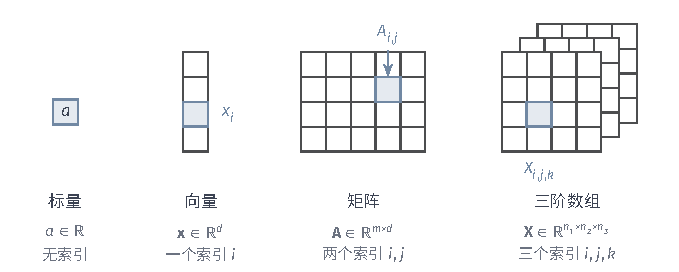
\includegraphics[width=112mm]{figures/01-mathematical-preliminaries-upper/03-linear-spaces/tikz/comprehension-additions/scalar-vector-matrix-tensor.pdf}
  \caption{标量、向量、矩阵与三阶数组的区别。每个面板用蓝色标出一个数：标量本身就是这个数，向量用一个索引$i$定位，矩阵用行列两个索引$i,j$定位，三阶数组再加一个索引$k$选择切片。索引个数称为阶，各轴长度组成形状。}
  \label{fig:ls-scalar-vector-matrix-tensor}
\end{figure}

两个同形数组按位置逐项相加、数乘，规则与向量、矩阵完全相同；两个数组能否相加，仍要求形状相同、对应轴的含义相同。使用多维数组时，须先说清每条轴记录什么：同一个$b\times\ell\times d$数组，若把第二、三轴的含义弄反，后续的每一次汇总都会汇总错的轴。

\subsection{张量的运算}
\label{sec:ls-tensor-operations}

多轴数组的运算按对轴的作用分成三类。轴置换与形状重整只改变元素记录在哪条轴、哪个位置上，不改变数值，也不求和。张量积和它的矩阵形式Kronecker积把多个因子的轴全部保留下来，组合成轴更多的数组。缩约则反过来，指定一对或几对轴对齐相乘后求和，把数组汇总成更低阶的数组。

\subsubsection{轴置换}
\label{sec:ls-tensor-reshaping}
\phantomsection
\label{sec:linear-algebra-tensors-structured-operations}

\term{维度重排}（permutation of axes）按给定顺序调换轴的位置，元素跟随自己的索引移动。计算时先写出新旧索引的对应，再按对应搬运元素。例如把$\bm X\in\mathbb R^{b\times\ell\times d}$的第二、三轴互换，得到$\bm Y\in\mathbb R^{b\times d\times\ell}$，
\[
 y_{i,k,j}=x_{i,j,k}.
\]
第一个轴保持原位，每个样本的切片被转置：$\bm Y_{i,:,:}=(\bm X_{i,:,:})^\top$。下面取一个具体的小数组。
\begin{example}[交换后两条轴]
\label{ex:ls-axis-swap}
给定：$b=1$、$\ell=2$、$d=3$，唯一的样本切片为$\bm X_{1,:,:}=\left[\begin{smallmatrix}1&2&3\\4&5&6\end{smallmatrix}\right]$。
计算：按$y_{1,k,j}=x_{1,j,k}$搬运元素，例如$y_{1,3,2}=x_{1,2,3}=6$，得到
\[
 \bm Y_{1,:,:}=\begin{bmatrix}1&4\\2&5\\3&6\end{bmatrix}.
\]
结论：$\bm Y\in\mathbb R^{1\times3\times2}$，它的样本切片正是原切片的转置。
\end{example}
矩阵的转置是两个轴时唯一的非平凡轴置换。轴的含义跟着轴走，不因位置改变而改变：$\bm Y$的第二轴仍是特征，第三轴仍是位置。

\subsubsection{形状重整与向量化}

\term{形状重整}（reshape）先按指定的遍历顺序把全部元素读成一个数列，再把这个数列按同样的顺序装入另一形状；它只要求元素总数相同。计算分两步：读出、装入。下面的例子比较按行重整与转置。
\begin{example}[按行重整与转置的区别]
\label{ex:ls-reshape-vs-transpose}
给定：$\bm A=\left[\begin{smallmatrix}1&2&3\\4&5&6\end{smallmatrix}\right]$，目标形状为$3\times2$。
计算：按行读出得数列$1,2,3,4,5,6$，再按行装入$3\times2$数组，得到
\[
 \bm R=\begin{bmatrix}1&2\\3&4\\5&6\end{bmatrix},
 \qquad\text{而}\qquad
 \bm A^\top=\begin{bmatrix}1&4\\2&5\\3&6\end{bmatrix}.
\]
结论：$\bm R$与$\bm A^\top$形状相同、所含的数相同，排列却不同。
\end{example}
所以重整不能只给目标形状，还要给遍历顺序；形状相同也不能说明完成了轴交换。图~\ref{fig:vol1-add-linear-transpose-reshape}把两种结果并排放置。
\begin{figure}[!htb]
  \centering
  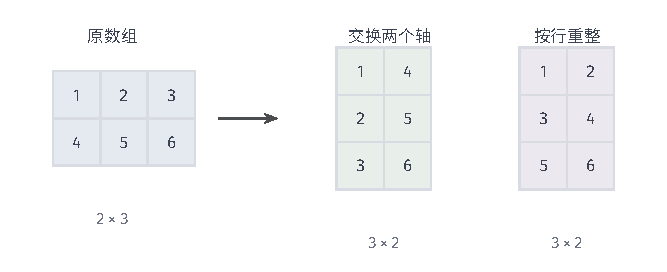
\includegraphics[width=112mm]{figures/01-mathematical-preliminaries-upper/03-linear-spaces/tikz/comprehension-additions/linear-transpose-reshape.pdf}
  \caption{轴交换与按行重整。原数组两行为$(1,2,3)$与$(4,5,6)$；中图转置后两列分别保留原来的两行，右图则把按行读取的数列$1,2,3,4,5,6$依次装入$3\times2$数组。数字及其排列由正文示例直接给出。}
  \label{fig:vol1-add-linear-transpose-reshape}
\end{figure}

形状重整中最常用的一种，是把矩阵按列堆叠成一个长列向量，称为\term{向量化}（vectorization）：
\[
 \operatorname{vec}(\bm A)=(a_{1,1},\ldots,a_{m,1},a_{1,2},\ldots,a_{m,2},\ldots,a_{1,n},\ldots,a_{m,n})^\top,
\]
$m\times n$矩阵的元素$a_{i,j}$位于一维索引$i+(j-1)m$。例如上面的$\bm A$给出$\operatorname{vec}(\bm A)=(1,4,2,5,3,6)^\top$，其中$a_{2,3}=6$位于第$2+(3-1)\cdot2=6$个位置。

多维数组也可以按轴重整成矩阵，称为矩阵展开（unfolding）：把一部分轴合并成行索引，其余轴合并成列索引。例如把$\bm X\in\mathbb R^{b\times\ell\times d}$的前两轴合并为行，得到$b\ell\times d$矩阵，每行是一个样本在一个位置上的特征。选哪些轴合并，决定展开结果的形状，也决定后续乘积汇总哪个轴。

\subsubsection{张量积}
\label{sec:ls-tensor-products}
\phantomsection
\label{sec:linear-algebra-joint-operations}

两个向量的全部两两乘积排成一个数组，就是它们的张量积。设$\bm x\in\mathbb R^m$、$\bm y\in\mathbb R^n$，\term{张量积}（tensor product）$\bm x\otimes\bm y$是$m\times n$数组，
\[
 (\bm x\otimes\bm y)_{i,j}=x_i y_j.
\]
写成矩阵，$\bm x\otimes\bm y=\bm x\bm y^\top$，正是分块乘法式~\eqref{eq:ls-product-outer-sum}中“一列乘一行”的矩阵。每个因子各占结果的一条轴，下面称为一个槽位。三个向量的张量积$(\bm x\otimes\bm y\otimes\bm z)_{i,j,k}=x_i y_j z_k$保留三个槽位，多重张量积按同样规则逐槽位相乘。下面计算两个二维向量的张量积。
\begin{example}[两个二维向量的张量积]
\label{ex:ls-tensor-product-two-vectors}
给定：$\bm x=(1,2)^\top$，$\bm y=(3,-1)^\top$。
计算：
\[
 \bm x\otimes\bm y=\begin{pmatrix}1\cdot3&1\cdot(-1)\\2\cdot3&2\cdot(-1)\end{pmatrix}=\begin{pmatrix}3&-1\\6&-2\end{pmatrix}.
\]
结论：第$i$行是$x_i\bm y^\top$，所以每一行都是$\bm y^\top$的倍数；同理，每一列都是$\bm x$的倍数。
\end{example}
图~\ref{fig:ls-tensor-product-slots}展示张量积怎样保留两个因子的槽位。
\begin{figure}[htbp]
  \centering
  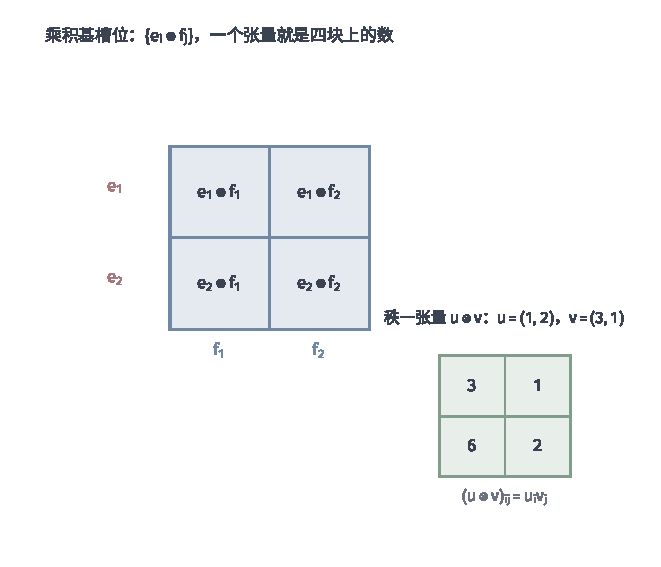
\includegraphics[width=112mm]{figures/01-mathematical-preliminaries-upper/03-linear-spaces/matplotlib/ls-tensor-product-slots/ls-tensor-product-slots.pdf}
  \caption{张量积并排保留两个因子的槽位。左：$\bm u\in\mathbb R^2$、$\bm v\in\mathbb R^3$。右：$\bm u\otimes\bm v$排成$2\times3$网格，每行由$\bm v$方向复制并按$u_i$缩放；它是简单张量，数值由$\bm u=(1,0.6)$、$\bm v=(1,0.5,0.2)$直接相乘得到，是教学构造。}
  \label{fig:ls-tensor-product-slots}
\end{figure}

形如$\bm x\otimes\bm y$的数组称为\term{简单张量}（simple tensor）。由示例~\ref{ex:ls-tensor-product-two-vectors}的结论，简单张量的各行都是同一个向量的倍数。并非每个二阶数组都是简单张量，下面是一个反例。
\begin{example}[反例：单位矩阵不是简单张量]
\label{ex:ls-identity-not-simple}
给定：$\bm I_2$，它的两行为$(1,0)$与$(0,1)$。
验证：若$\bm I_2=\bm x\otimes\bm y$，则两行分别是$x_1\bm y^\top$与$x_2\bm y^\top$。两行都非零，所以$x_1,x_2\neq0$，两行都是$\bm y^\top$的非零倍数，从而彼此成比例。但$(1,0)$与$(0,1)$不成比例。
结论：$\bm I_2$不能写成任何$\bm x\otimes\bm y$，它不是简单张量。
\end{example}
不过，每个$m\times n$数组$\bm T$都是简单张量的和，
\[
 \bm T=\sum_{i,j}t_{i,j}\,\bm e_i\otimes\bm f_j,
\]
其中$\bm e_i$、$\bm f_j$分别是$\mathbb R^m$与$\mathbb R^n$的标准坐标向量，$\bm e_i\otimes\bm f_j$只在位置$(i,j)$为$1$。

张量积的用处，是把同时依赖两组输入的读取化为对单个数组的线性读取。设实值函数$B(\bm x,\bm y)$对$\bm x$、$\bm y$分别保持线性组合（称为双线性）。把$\bm x=\sum_ix_i\bm e_i$、$\bm y=\sum_jy_j\bm f_j$代入，按两次线性展开，
\[
 B(\bm x,\bm y)=\sum_{i,j}x_iy_j\,B(\bm e_i,\bm f_j)=\sum_{i,j}g_{i,j}(\bm x\otimes\bm y)_{i,j}
 =\langle\bm G,\bm x\otimes\bm y\rangle_{\mathrm F},
\]
其中$g_{i,j}=B(\bm e_i,\bm f_j)$。所以双线性读取由一张固定的系数表$\bm G$决定，并且它对数组$\bm x\otimes\bm y$是线性的。以欧氏内积$B(\bm x,\bm y)=\bm x^\top\bm y$（$m=n$）为例，$g_{i,j}=\langle\bm e_i,\bm e_j\rangle$，即$\bm G=\bm I$，读取就是把$\bm x\otimes\bm y$的对角线加起来。

二阶张量与矩阵是同一组数的两种记录：张量强调槽位来自哪一组输入，矩阵强调行列在乘法中的角色。

\subsubsection{Kronecker积}

两个矩阵分别作用在两条轴上时，联合作用可以写成一张大矩阵。对$\bm A\in\mathbb R^{m\times n}$、$\bm B\in\mathbb R^{p\times q}$，定义Kronecker积
\begin{equation}
 \bm A\otimes\bm B
 =\begin{bmatrix}
  A_{1,1}\bm B&\cdots&A_{1,n}\bm B\\
  \vdots&\ddots&\vdots\\
  A_{m,1}\bm B&\cdots&A_{m,n}\bm B
 \end{bmatrix}\in\mathbb R^{mp\times nq}.
 \label{eq:linear-algebra-kronecker-product}
\end{equation}
计算时把$\bm A$的每个元素$A_{i,j}$替换成块$A_{i,j}\bm B$。下面计算一个二阶的例子。
\begin{example}[两个二阶矩阵的Kronecker积]
\label{ex:ls-kronecker-two-by-two}
给定：$\bm A=\left[\begin{smallmatrix}1&2\\3&4\end{smallmatrix}\right]$，$\bm B=\left[\begin{smallmatrix}0&1\\1&0\end{smallmatrix}\right]$。
计算：
\[
 \bm A\otimes\bm B
 =\begin{bmatrix}
  1\cdot\bm B&2\cdot\bm B\\
  3\cdot\bm B&4\cdot\bm B
 \end{bmatrix}
 =\begin{bmatrix}0&1&0&2\\1&0&2&0\\0&3&0&4\\3&0&4&0\end{bmatrix}.
\]
结论：$\bm A\otimes\bm B$是$4\times4$矩阵，四个$2\times2$块依次是$\bm B$的$1,2,3,4$倍。
\end{example}
图~\ref{fig:ls-kronecker-block-structure}用另一组数展示这种逐元素替换的分块结构。
\begin{figure}[htbp]
  \centering
  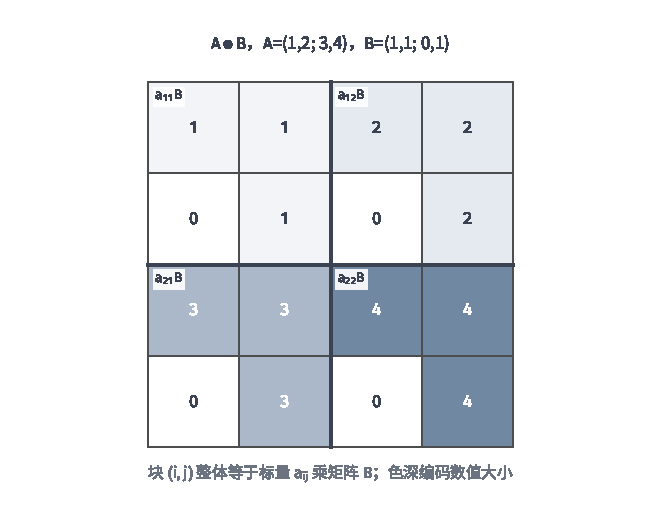
\includegraphics[width=112mm]{figures/01-mathematical-preliminaries-upper/03-linear-spaces/matplotlib/ls-kronecker-block-structure/ls-kronecker-block-structure.pdf}
  \caption{Kronecker积的分块结构。上：$\bm A=\bigl(\begin{smallmatrix}1&2\\3&4\end{smallmatrix}\bigr)$、$\bm B=\bigl(\begin{smallmatrix}10&20\\30&40\end{smallmatrix}\bigr)$。下：$\bm A\otimes\bm B$是把$\bm A$的每个元素替换为该元素乘$\bm B$得到的$4\times4$分块矩阵，块边界用白线强调。数值由定义直接计算，是教学例。}
  \label{fig:ls-kronecker-block-structure}
\end{figure}

两个列向量按式~\eqref{eq:linear-algebra-kronecker-product}相乘，得到$mn$维长向量$(x_1\bm y^\top,\ldots,x_m\bm y^\top)^\top$，它正是把$m\times n$数组$\bm x\otimes\bm y$按行读出的结果。两种用法记录的是同一组数，只差一次按行读出，所以同一个记号$\otimes$不会引起混淆。例如$(1,2)^\top\otimes(3,-1)^\top=(3,-1,6,-2)^\top$，与示例~\ref{ex:ls-tensor-product-two-vectors}中的数组按行读出的结果相同。

\subsubsection{张量缩约}
\label{sec:ls-tensor-contraction}

张量积把槽位全部保留；缩约则沿指定的轴汇总。计算时选定一对或几对尺寸相同的轴，让每对轴共用同一个求和索引，逐项相乘后对这些索引求和；被求和的轴消失，其余轴保留，按原次序组成输出的形状。写出索引，就能检查哪些轴被消去、哪些轴应当保留，下面用两个例子说明这种检查。
\begin{example}[两种缩约的输出形状]
\label{ex:ls-contraction-shapes}
给定：（1）$\bm A\in\mathbb R^{m\times d\times r}$与$\bm B\in\mathbb R^{d\times n\times r}$；（2）$\bm X\in\mathbb R^{b\times\ell\times d}$与$\bm W\in\mathbb R^{d\times h}$。
计算：（1）让$\bm A$的第二轴与$\bm B$的第一轴共用索引$k$，两者的第三轴共用索引$s$，
\[
 c_{i,j}=\sum_{k=1}^d\sum_{s=1}^r a_{i,k,s}b_{k,j,s}.
\]
（2）让$\bm X$的最后一轴与$\bm W$的第一轴共用索引$k$，
\[
 z_{i,j,t}=\sum_{k=1}^d x_{i,j,k}w_{k,t}.
\]
结论：（1）同时消去$k$与$s$两对轴，保留$i,j$，输出为$m\times n$矩阵。（2）只消去$k$，保留$i,j,t$，输出形状为$b\times\ell\times h$：每个样本、每个位置上的$d$维特征都乘了同一个矩阵$\bm W$。
\end{example}
图~\ref{fig:ls-tensor-contraction}沿一对选中的轴求和并保留其余轴。
\begin{figure}[htbp]
  \centering
  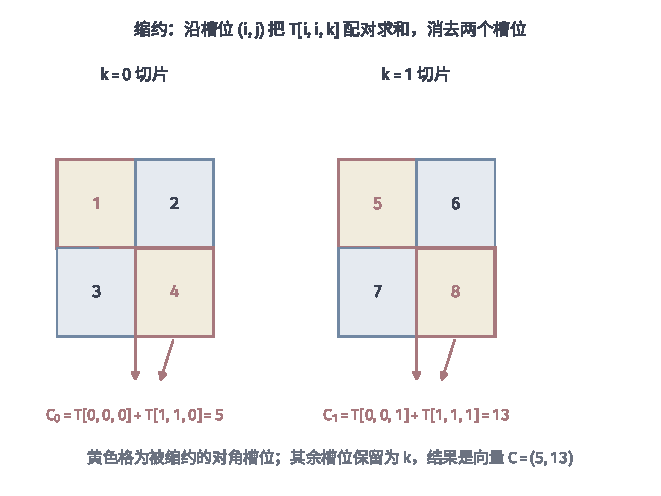
\includegraphics[width=112mm]{figures/01-mathematical-preliminaries-upper/03-linear-spaces/matplotlib/ls-tensor-contraction/ls-tensor-contraction.pdf}
  \caption{张量缩约沿选中的一对轴求和、保留其余轴。左：二阶张量按行和列着色；选中列轴（虚线箭头）沿列求和，输出对每行汇总为一个值。右：缩约后得到$3$个输出，分别对应原矩阵三行的行和，颜色由红（小）经黄到蓝（大）。张量与数值均为解析教学例。}
  \label{fig:ls-tensor-contraction}
\end{figure}

前两节的几种运算都是缩约：
\begin{itemize}
 \item 内积$\sum_jx_jy_j$缩约两个向量唯一的一对轴，输出标量；
 \item 矩阵乘法$\sum_\ell a_{i,\ell}b_{\ell,j}$只消去左因子的列轴与右因子的行轴这一对；
 \item 迹$\sum_iA_{i,i}$把同一个矩阵的行轴与列轴对齐到同一索引后求和；
 \item Frobenius内积$\sum_{i,j}a_{i,j}b_{i,j}$同时缩约两对轴。
\end{itemize}

\subsection{张量运算的性质}
\label{sec:ls-tensor-operation-properties}

使用上一小节的运算时，须知道哪些操作可以撤销、括号怎样移动、Kronecker积怎样与普通矩阵乘法配合，以及缩约何时可以分开计算。本小节按运算整理，最后用一张表汇总各种“乘法”的形状条件。

\subsubsection{重排的性质}

\paragraph{可逆性}
目标形状与遍历顺序固定后，轴置换、形状重整与向量化都把一个数组一一对应到另一个数组，逆操作恢复原数组：转置再转置、按逆置换换回、按原顺序装回。例如$\operatorname{vec}$的逆操作把长度为$mn$的向量依次每$m$个一列装回$m\times n$矩阵。所以重排保留全部信息。

\paragraph{线性}
\[
 \operatorname{vec}(a\bm A+b\bm B)=a\operatorname{vec}(\bm A)+b\operatorname{vec}(\bm B),
\]
轴置换与形状重整同样满足这一性质：它们只搬动元素，逐项的加法与数乘搬到新位置后不变。

\paragraph{与矩阵乘法的关系}
转置与乘法有整齐的规则$(\bm A\bm B)^\top=\bm B^\top\bm A^\top$；一般的形状重整与乘法没有这样的关系。重整以后，矩阵每一行、每一列汇集的元素都变了，依赖行列结构的乘积、迹与行列式一般随之改变。下面的反例把示例~\ref{ex:ls-reshape-vs-transpose}中的$\bm R$误当作$\bm A^\top$使用。
\begin{example}[反例：重整不能代替转置]
\label{ex:ls-reshape-breaks-product}
给定：$\bm A=\left[\begin{smallmatrix}1&2&3\\4&5&6\end{smallmatrix}\right]$，以及按行重整得到的$\bm R=\left[\begin{smallmatrix}1&2\\3&4\\5&6\end{smallmatrix}\right]$。
计算：由示例~\ref{ex:ls-gram-product-symmetric}，$\bm A\bm A^\top=\left[\begin{smallmatrix}14&32\\32&77\end{smallmatrix}\right]$；而
\[
 \bm A\bm R=\begin{bmatrix}1+6+15&2+8+18\\4+15+30&8+20+36\end{bmatrix}=\begin{bmatrix}22&28\\49&64\end{bmatrix}.
\]
结论：$\bm R$与$\bm A^\top$形状相同、所含的数相同，两个乘积的迹却分别为$14+77=91$与$22+64=86$。
\end{example}
把存储格式的改变当成计算效果，是这里最常见的错误。

\subsubsection{张量积的性质}

\paragraph{对每个因子线性}
\[
 (a\bm x)\otimes\bm y=\bm x\otimes(a\bm y)=a(\bm x\otimes\bm y),\qquad
 (\bm x+\bm x')\otimes\bm y=\bm x\otimes\bm y+\bm x'\otimes\bm y,
\]
对第二个因子的加法同样分配。每个元素$x_iy_j$对$x_i$和$y_j$分别线性，逐项验证即得。

\paragraph{结合律}
\[
 (\bm x\otimes\bm y)\otimes\bm z=\bm x\otimes(\bm y\otimes\bm z),
\]
两边的$(i,j,k)$元素都是$x_iy_jz_k$。

\paragraph{交换槽位是转置}
\[
 \bm y\otimes\bm x=(\bm x\otimes\bm y)^\top,
\]
因为$\bm x\otimes\bm y$的$(i,j)$元素$x_iy_j$也是$\bm y\otimes\bm x$的$(j,i)$元素。所以一般$\bm x\otimes\bm y\neq\bm y\otimes\bm x$，两者相差一次轴置换。

\paragraph{Frobenius配对与范数分离}
\[
 \langle\bm x\otimes\bm y,\bm x'\otimes\bm y'\rangle_{\mathrm F}
 =\langle\bm x,\bm x'\rangle\langle\bm y,\bm y'\rangle,
 \qquad
 \lVert\bm x\otimes\bm y\rVert_{\mathrm F}=\lVert\bm x\rVert_2\,\lVert\bm y\rVert_2.
\]
第一式来自$\sum_{i,j}x_iy_jx'_iy'_j=(\sum_ix_ix'_i)(\sum_jy_jy'_j)$；第二式在第一式中取$\bm x'=\bm x$、$\bm y'=\bm y$后开平方。下面在示例~\ref{ex:ls-tensor-product-two-vectors}的数组上核对第二式。
\begin{example}[张量积范数的数值核对]
\label{ex:ls-tensor-product-norm-check}
给定：$\bm x=(1,2)^\top$，$\bm y=(3,-1)^\top$，$\bm x\otimes\bm y=\left(\begin{smallmatrix}3&-1\\6&-2\end{smallmatrix}\right)$。
计算：$\lVert\bm x\rVert_2=\sqrt5$，$\lVert\bm y\rVert_2=\sqrt{10}$；直接求Frobenius范数，
\[
 \lVert\bm x\otimes\bm y\rVert_{\mathrm F}=\sqrt{3^2+(-1)^2+6^2+(-2)^2}=\sqrt{50}.
\]
结论：$\sqrt5\cdot\sqrt{10}=\sqrt{50}=5\sqrt2$，两种算法一致。
\end{example}

\paragraph{与楔积的联系}
矩阵一节的楔积也可以由张量积经反对称化得到：$\bm x\wedge\bm y$对应$\bm x\otimes\bm y-\bm y\otimes\bm x$，交换$\bm x,\bm y$时它变号。这里只指出联系，楔积的规则不依赖张量积。

\subsubsection{Kronecker积的性质}
\label{sec:ls-kronecker-products}

\paragraph{分别作用于两个槽位}
\[
 (\bm A\otimes\bm B)(\bm x\otimes\bm y)=(\bm A\bm x)\otimes(\bm B\bm y).
\]
按分块乘法，左侧第$i$块为$\sum_jA_{i,j}\bm B(x_j\bm y)=(\sum_jA_{i,j}x_j)\bm B\bm y=(\bm A\bm x)_i\,\bm B\bm y$，正是右侧的第$i$块。第一个槽位只经过$\bm A$，第二个槽位只经过$\bm B$，两个作用并行而不串联；矩阵乘法则把前后两次作用串成一条链。

\paragraph{混合乘积}
当$\bm A\bm C$与$\bm B\bm D$分别有定义时，
\begin{equation}
 (\bm A\otimes\bm B)(\bm C\otimes\bm D)
 =(\bm A\bm C)\otimes(\bm B\bm D).
 \label{eq:matrix-analysis-kronecker-mixed-product}
\end{equation}
按分块乘法，左侧的块$(i,k)$为$\sum_j(A_{i,j}\bm B)(C_{j,k}\bm D)=(\sum_jA_{i,j}C_{j,k})\bm B\bm D=(\bm A\bm C)_{i,k}\bm B\bm D$，恰是右侧的块。上一条是$\bm C,\bm D$各只有一列的情形。

\paragraph{转置}
\[
 (\bm A\otimes\bm B)^\top=\bm A^\top\otimes\bm B^\top.
\]
分块矩阵转置时，块的位置交换，每块各自转置，所以第$(j,i)$块为$A_{i,j}\bm B^\top$，正是$\bm A^\top\otimes\bm B^\top$的第$(j,i)$块。

\paragraph{逆}
\[
 (\bm A\otimes\bm B)^{-1}=\bm A^{-1}\otimes\bm B^{-1}\qquad(\bm A,\bm B\text{都可逆}).
\]
由混合乘积，$(\bm A\otimes\bm B)(\bm A^{-1}\otimes\bm B^{-1})=(\bm A\bm A^{-1})\otimes(\bm B\bm B^{-1})=\bm I\otimes\bm I=\bm I$，另一侧同理。

\paragraph{迹}
\[
 \operatorname{tr}(\bm A\otimes\bm B)=\operatorname{tr}\bm A\,\operatorname{tr}\bm B\qquad(\bm A,\bm B\text{都是方阵}).
\]
只有对角块$A_{i,i}\bm B$的对角元落在主对角线上，所以迹为$\sum_iA_{i,i}\operatorname{tr}\bm B=\operatorname{tr}\bm A\,\operatorname{tr}\bm B$。

\paragraph{向量化恒等式}
对$\bm A\in\mathbb R^{p\times m}$、$\bm X\in\mathbb R^{m\times n}$、$\bm B\in\mathbb R^{n\times q}$，
\begin{equation}
 \operatorname{vec}(\bm A\bm X\bm B)
 =(\bm B^\top\otimes\bm A)\operatorname{vec}(\bm X).
 \label{eq:matrix-analysis-vec-kronecker}
\end{equation}
比较两侧输出的第$j$段（长度为$p$）。左侧是$\bm A\bm X\bm B$的第$j$列，$\bm A\bm X\bm B_{:,j}=\sum_kB_{k,j}\bm A\bm X_{:,k}$。右侧矩阵的第$j$块行为$(B_{1,j}\bm A,\ldots,B_{n,j}\bm A)$，与$\operatorname{vec}(\bm X)$的各段$\bm X_{:,1},\ldots,\bm X_{:,n}$相乘，也得到$\sum_kB_{k,j}\bm A\bm X_{:,k}$。逐元素写出，两侧$(i,j)$位置的元素都是$\sum_{\ell=1}^m\sum_{k=1}^n A_{i,\ell}X_{\ell,k}B_{k,j}$。

固定$\bm A,\bm B$后，这一恒等式把“两侧同时乘矩阵”写成对长向量$\operatorname{vec}(\bm X)$乘一张矩阵，从而把关于未知矩阵的方程化成普通线性方程组；第~\ref{chap:linear-equations-and-optimization}章求解矩阵方程时将用到它。

\subsubsection{缩约的性质}

\paragraph{线性}
固定配对数组后，缩约对被作用数组线性：把被作用数组换成$a\bm X+b\bm X'$，输出变为$a$倍与$b$倍两个输出之和。这是因为每个输出元素都是被作用数组元素以固定系数作的加权和。

\paragraph{求和次序可交换}
多对轴的缩约是有限和，结果与先消哪一对轴无关。例如示例~\ref{ex:ls-contraction-shapes}中的$c_{i,j}$可以先对$s$求和得到中间数组，再对$k$求和，也可以反过来。

\paragraph{简单张量系数可分离}
一次读取同时依赖三组向量$\bm x\in\mathbb R^m$、$\bm y\in\mathbb R^n$、$\bm z\in\mathbb R^p$时，若系数数组是简单张量$\bm a\otimes\bm b\otimes\bm c$，则
\begin{equation}
 \left\langle\bm a\otimes\bm b\otimes\bm c,
 \bm x\otimes\bm y\otimes\bm z\right\rangle_{\mathrm F}
 =(\bm a^\top\bm x)(\bm b^\top\bm y)(\bm c^\top\bm z),
 \label{eq:linear-algebra-rank-one-contraction}
\end{equation}
因为$\sum_{i,j,k}a_ib_jc_kx_iy_jz_k=(\sum_ia_ix_i)(\sum_jb_jy_j)(\sum_kc_kz_k)$：三重求和分离成三个内积的乘积，计算量从$mnp$项降到$m+n+p$项。下面用一组小数值核对。
\begin{example}[简单张量系数的分离计算]
\label{ex:ls-rank-one-contraction-check}
给定：$\bm a=(1,2)^\top$、$\bm b=(3,-1)^\top$、$\bm c=(2,1)^\top$，$\bm x=(2,1)^\top$、$\bm y=(1,1)^\top$、$\bm z=(1,-1)^\top$，这里$m=n=p=2$。
计算：三个内积依次为
\[
 \begin{gathered}
 \bm a^\top\bm x=1\cdot2+2\cdot1=4,\qquad
 \bm b^\top\bm y=3\cdot1+(-1)\cdot1=2,\\
 \bm c^\top\bm z=2\cdot1+1\cdot(-1)=1.
 \end{gathered}
\]
结论：由式~\eqref{eq:linear-algebra-rank-one-contraction}，读取等于$4\cdot2\cdot1=8$；直接展开三重求和要累加$2^3=8$项乘积，结果同样是$8$。
\end{example}

\paragraph{非线性操作不是缩约}
$\operatorname{softmax}$、逐元素非线性等操作不属于缩约。一个模型即使由缩约和这些操作交替组成，固定系数时每一步缩约的线性也不代表整体线性。

\subsubsection{各种乘积的形状}

本章出现了好几种“乘法”，它们的区别在于对索引做什么。表~\ref{tab:linear-algebra-products-and-shapes}汇总它们的形状条件与索引作用。

\begin{table*}[htbp]
 \centering\small
 \begin{tabularx}{\linewidth}{@{}lXX@{}}
  \toprule
  运算 & 形状条件与输出 & 索引作用\\
  \midrule
  $\langle\bm x,\bm y\rangle$ & 两个$n$维向量，输出标量 & 配对后汇总\\
  $\bm A\bm B$ & $(m\times n)(n\times p)\to m\times p$ & 汇总共同索引\\
  $\bm A\odot\bm B$ & 同为$m\times n$，输出仍为$m\times n$ & 同位置相乘，不求和\\
  $\bm x\otimes\bm y$ & $m$维与$n$维向量$\to m\times n$ & 保留两条轴，不求和\\
  $\bm A\otimes\bm B$ & $(m\times n)$与$(p\times q)\to(mp)\times(nq)$ & 保留两组成对索引\\
  缩约 & 被缩约的各对轴尺寸相同 & 消去指定轴，保留其余轴\\
  \bottomrule
 \end{tabularx}
 \caption{相乘符号对应不同操作。先检查消去哪些索引，再判断其线性性和输出含义。}
 \label{tab:linear-algebra-products-and-shapes}
\end{table*}

% 第4章：本章小结。

\section{本章小结}
\label{sec:ls-operations-summary}

本章按定位一个数所需的索引个数，依次处理向量、矩阵与张量，并对每种运算交代输入条件、输出形状和可用的规则。向量的加法与数乘合成线性组合；内积把两个向量配成一个数，范数用四条公理统一各种误差口径，由内积给出的欧氏范数还满足平行四边形恒等式。

矩阵乘积来自两次加权求和的复合，满足结合律与分配律，却不满足交换律与消去律；逆矩阵撤销一次乘法，矩阵幂记录反复作用。迹、行列式与矩阵范数把矩阵读成一个数：行列式是有向体积的缩放倍数，诱导范数是最坏情形的放大倍数。张量把索引推广到任意多个：重排只改变元素位置，张量积保留全部槽位，缩约沿指定的轴求和，内积、矩阵乘积与迹都是缩约的特例。

本章只把这些数组当作具体的数表。第~\ref{chap:linear-representation}章接着追问它们记录的是什么：同一个对象换一组方向后坐标怎样改变，矩阵怎样记录线性映射，一般空间中的夹角与正交怎样讨论。矩阵反复作用的走向与误差的放大留给第~\ref{chap:linear-analysis}章，方程怎样求解留给第~\ref{chap:linear-equations-and-optimization}章。


\chapter{线性空间}
\label{chap:linear-representation}
\label{chap:linear-algebra-and-matrix-analysis}
\label{chap:linear-algebra}

第~\ref{chap:linear-operations}章把数据记成数组，并规定了数组之间的运算，但始终没有追问数组记录的是什么。同一区间上的仿射函数$f_{a,b}(t)=a+bt$是一个完整的函数，两个这样的函数相加、缩放后仍是仿射函数。只有选定$1$与$t$这两个“方向”以后，它才被记录成一列数$(a,b)^{\top}$；换一组方向，记录的数就跟着改变，函数本身却不变。设计矩阵$\bm X_\varepsilon$（式~\eqref{eq:linear-algebra-nearly-collinear-design}）也是如此：它既是一张$3\times2$的数表，也记录了一个把两个系数送到三个拟合值的作用。要在不同记录之间换算而不被记录方式误导，必须把对象与记录对象的数分开。

本章围绕这一区分回答六组问题。第一，哪些对象可以放在一起作线性组合，一个空间里哪些部分自己也构成空间，忽略某个部分里的差别以后还剩下什么？第二，怎样挑出一组既够用又不重复的方向当作“尺子”，尺子需要几根；选定尺子以后，对象怎样记录成坐标，换一把尺子坐标怎样换算？第三，保持线性组合的作用怎样记录成矩阵，它丢失了哪些输入信息、能到达哪些输出，什么时候可以撤销；换一把尺子，记录作用的矩阵怎样改变，哪些量不随之改变？第四，把对象读成一个数的规则本身组成怎样的空间，经过一个作用以后读取怎样传回输入端？第五，一般空间上怎样度量大小，一列近似什么时候收敛，极限是否仍在空间中？第六，一般空间上的内积怎样规定、选基以后怎样计算；有了内积以后，空间怎样按互相垂直的方向分解，怎样找到一把互相垂直的尺子？

这些问题按依赖关系排列，后一节总在前一节已有的结构上工作。前四节的主线只用加法与数乘。线性空间与子空间（第~\ref{sec:ls-vector-spaces}节）规定可以讨论的对象；基、维数与坐标（第~\ref{sec:ls-bases-dimension-coordinates}节）给出记录对象的语言；线性映射（第~\ref{sec:ls-linear-maps}节）用这种语言把作用记录成矩阵，第~\ref{chap:linear-operations}章的矩阵乘法与逆矩阵在这里得到含义，矩阵的四个基本子空间也在这里定义，并借核与像求出它们的维数。对偶空间（第~\ref{sec:ls-dual-spaces}节）讨论线性映射的一个特例，即把对象映成一个数的读取；它给转置一个不依赖坐标的含义，并在最后借$\mathbb R^d$上的范数给出读取的大小。

后两节加入度量。赋范空间（第~\ref{sec:ls-normed-spaces}节）加入长度，从而可以讨论收敛与完备性；有限维中一切范数等价，收敛就是逐坐标收敛。内积空间（第~\ref{sec:ls-inner-product-spaces}节）在长度之外再加入角度。内积诱导范数，所以这一节放在赋范空间之后；内积又把读取识别为向量，把对偶映射变成伴随，所以它也放在对偶空间之后。第~\ref{chap:linear-operations}章在$\mathbb R^d$上建立的内积、正交与正交矩阵在这里推广到一般空间，Cauchy--Schwarz不等式与夹角也在这里建立，完备的内积空间即Hilbert空间。同一空间上反复施加的作用在哪些方向上最简单，即特征值与对角化，留到第~\ref{chap:linear-analysis}章。

% 第5章第1节：线性空间的定义（向量空间；子空间及其包含、交、和、直和与商空间）。

\section{线性空间的定义}
\label{sec:ls-vector-spaces}
\label{sec:linear-algebra-vector-spaces-coordinates}

第~\ref{chap:linear-operations}章的向量与矩阵、本章开头的仿射函数都可以相加和缩放。要用一组方向去记录这些对象，先得说清楚记录在什么范围里进行。本节回答两个问题。第一，哪些对象可以放在一起作线性组合，并且结果仍是同类对象；这由向量空间的定义回答。第二，在这样的空间内部，哪些部分自己也能作线性组合而不越界，几个这样的部分怎样比较与合并，有意忽略某个部分里的差别以后又剩下什么；这由子空间及其运算回答。怎样在一个空间里选出一组“尺子”、空间有多大，是下一节的问题。

\subsection{向量空间}
\label{sec:ls-space-axioms}

第~\ref{sec:ls-vector-operation-rules}节验证过，同形数组的加法与数乘满足八条运算规则。平面上的位移可以首尾相接，有限信号可以按幅度放大，多项式可以逐点相加，它们同样满足这些规则：两个对象可以相加，一个对象可以乘以实数，结果仍是同类对象，运算按熟悉的方式交换、结合与分配。后面关于“能否分解、方程有无解、维数是多少”的结论只用到这些规则，与对象具体是数组、位移、信号还是多项式无关。因此把满足这些规则的集合统称为线性空间，其中的元素统称为向量；“向量”从此指可以作线性组合的对象，不再要求它是一列数。

\begin{definition}[实线性空间]
\label{def:ls-real-vector-space}
设$V$是一个集合，给定加法（任意$\bm u,\bm v\in V$对应$\bm u+\bm v\in V$）与实数数乘（任意$a\in\mathbb R$、$\bm u\in V$对应$a\bm u\in V$）。若对任意$\bm u,\bm v,\bm w\in V$和$a,b\in\mathbb R$，下面八条规则成立，就称$V$为\term{向量空间}（也称线性空间，vector space）：
\begin{enumerate}
 \item 加法交换律：$\bm u+\bm v=\bm v+\bm u$。
 \item 加法结合律：$(\bm u+\bm v)+\bm w=\bm u+(\bm v+\bm w)$。
 \item 零元：存在$\bm0\in V$，使$\bm u+\bm0=\bm u$对每个$\bm u$成立。
 \item 加法逆元：每个$\bm u$都有$-\bm u\in V$，使$\bm u+(-\bm u)=\bm0$。
 \item 数乘结合律：$a(b\bm u)=(ab)\bm u$。
 \item 数乘对数的分配律：$(a+b)\bm u=a\bm u+b\bm u$。
 \item 数乘对向量的分配律：$a(\bm u+\bm v)=a\bm u+a\bm v$。
 \item 单位数乘：$1\bm u=\bm u$。
\end{enumerate}
\end{definition}
定义包含两层要求。第一层是\emph{封闭}：加法和数乘的结果必须留在$V$中，否则运算根本无法在$V$内进行。第二层是\emph{规则}：前四条说加法和数的加法一样可以交换、结合，有零元和相反元；后四条说数乘与加法按熟悉的方式配合。

有了这些规则，有限次线性运算无论怎样加括号、怎样展开，都给出同一结果。于是对任意$\bm v_1,\ldots,\bm v_k\in V$与实数$a_1,\ldots,a_k$，加权和$\sum_{j=1}^ka_j\bm v_j$都有确定的意义，仍称为这组向量的线性组合，与第~\ref{sec:ls-vector-operations}节对数组的定义一致。

常见的具体空间都满足定义。$\mathbb R^d$与全部$m\times d$实矩阵在逐项运算下是线性空间，第~\ref{sec:ls-vector-operation-rules}节已逐条验证。次数不超过$k$的实多项式组成的集合$P_k=\{a_0+a_1t+\cdots+a_kt^k\}$在逐点相加与数乘下也是线性空间：两个次数不超过$k$的多项式相加、乘以实数以后，次数仍不超过$k$，八条规则则逐点继承实数的运算规则。本章开头的仿射函数族正是$P_1$。

并非每个由向量组成的集合都是线性空间。下面两个$\mathbb R^d$的子集沿用$\mathbb R^d$的运算，却分别破坏了加法封闭与数乘封闭。
\begin{example}[反例：仿射约束集与非负向量集]
\label{ex:ls-non-vector-space-sets}
给定：$\mathbb R^d$的两个子集
\[
 S_1=\{\bm x\in\mathbb R^d:x_1=1\},
 \qquad
 S_2=\{\bm x\in\mathbb R^d:x_j\geq0,\ j=1,\ldots,d\},
\]
运算沿用$\mathbb R^d$的逐项加法与数乘。

验证：任取$\bm x,\bm y\in S_1$，和的第一坐标为$x_1+y_1=2\neq1$，所以$\bm x+\bm y\notin S_1$；零向量的第一坐标为$0$，所以$S_1$也不含零向量。对$S_2$，两个非负向量之和仍非负，加法封闭；但$\bm e_1\in S_2$，而$(-1)\bm e_1$的第一坐标为$-1$，所以$(-1)\bm e_1\notin S_2$。

结论：$S_1$对加法不封闭，$S_2$对数乘不封闭，二者都不是线性空间。
\end{example}
两个反例说明，判断一个集合是不是线性空间，要逐项检查运算是否封闭、规则是否成立，不能只看集合的形状。

\subsection{子空间}
\label{sec:ls-subspaces}
\label{sec:linear-algebra-relations}
\label{sec:linear-algebra-subspace-relations}
\label{sec:ls-subspace-definition}

线性空间$V$中常有一部分元素自己就构成线性空间，例如平面里过原点的一条直线、齐次方程组的全部解。后面的许多问题都落在这样的部分上：一组方向能到达的对象、一个作用消去的输入、方程的解，都不是整个空间。怎样判断$V$的一部分仍是线性空间？

\paragraph{子空间的判定}
设$U$是$V$的非空子集。若$U$对线性组合封闭，即对任意$\bm u,\bm v\in U$和$a,b\in\mathbb R$都有$a\bm u+b\bm v\in U$，就称$U$为$V$的\term{线性子空间}（linear subspace），简称子空间。这时$U$用$V$的加法与数乘也构成线性空间：取$a=b=1$与$b=0$，分别得到加法与数乘封闭；取$a=b=0$得$\bm0\in U$，取$a=-1,b=0$得$-\bm u\in U$；其余规则对$V$的全部元素成立，自然也对$U$的元素成立。所以判断子空间只需检查这一条封闭条件，不必逐条核对八条规则。

每个空间都有两个平凡子空间：只含零向量的$\{\bm0\}$和$V$本身。下面用判定条件检查三类常见集合。
\begin{example}[过原点的直线、平移的直线与齐次解集]
\label{ex:ls-subspace-checks}
给定：平面中的非零向量$\bm u$，不在直线$\{c\bm u:c\in\mathbb R\}$上的点$\bm p$，以及矩阵$\bm A\in\mathbb R^{m\times d}$。考察
\[
 \begin{gathered}
 L_0=\{c\bm u:c\in\mathbb R\},
 \qquad
 L_1=\{\bm p+c\bm u:c\in\mathbb R\},\\
 N=\{\bm x\in\mathbb R^d:\bm A\bm x=\bm0\}.
 \end{gathered}
\]

验证：在$L_0$中任取$c_1\bm u$与$c_2\bm u$，有$a(c_1\bm u)+b(c_2\bm u)=(ac_1+bc_2)\bm u\in L_0$。在$N$中任取两个解$\bm x,\bm y$，由式~\eqref{eq:prelim-matrix-linearity}，
\[
 \bm A(a\bm x+b\bm y)=a\bm A\bm x+b\bm A\bm y=\bm0,
\]
所以$a\bm x+b\bm y\in N$。$L_1$不含零向量：若$\bm p+c\bm u=\bm0$，则$\bm p=-c\bm u$落在$L_0$上，与$\bm p$的取法矛盾。

结论：过原点的直线$L_0$与齐次线性方程组的解集合$N$都是子空间；不过原点的直线$L_1$不含零向量，不是子空间。
\end{example}
$L_1$是子空间$L_0$沿$\bm p$平移所得。示例~\ref{ex:ls-non-vector-space-sets}中的非齐次约束集$S_1=\{\bm x:x_1=1\}$也是这样，它是齐次解集$\{\bm x:x_1=0\}$沿$\bm e_1$平移所得的仿射集合，同样不是子空间。

固定同一个空间$V$，它的几个子空间之间可以问四个问题：一个是否装得下另一个，二者有哪些公共方向，合在一起能到达哪里，合并后的分解是否唯一。这四个问题分别由包含、交、和与直和回答。这里比较的都是线性范围，不涉及长度或夹角。最后再问一个方向相反的问题：若把某个子空间里的差别有意忽略，剩下的对象是否仍构成线性空间？这由商空间回答。

\paragraph{包含}
\phantomsection
\label{sec:ls-subspace-inclusion}
若子空间$U$的每个元素都属于子空间$W$，就记$U\subseteq W$。这时$U$在$W$中对线性组合封闭，因而也是$W$的子空间。包含只比较两个集合的范围；两个子空间的“大小”怎样比较，要等下一节定义维数以后才能回答。

\paragraph{交}
\phantomsection
\label{sec:ls-intersection}
两个子空间$U,W\subseteq V$的交$U\cap W$由同时属于二者的元素组成。它仍是子空间：$\bm x,\bm y\in U\cap W$时，二者既在$U$中也在$W$中，故$a\bm x+b\bm y$同属两边。交也是同时包含在$U$与$W$中的最大子空间，因为任何同时含于两边的子空间，其元素都属于交。在平面中，两条重合的过原点直线的交是整条直线，两条不同的过原点直线的交只有零向量。交为零只说明两个子空间没有公共的非零方向，并不说明二者合起来能到达整个空间：$\mathbb R^3$中两条不同的过原点直线交为零，合起来却只能到达一个平面。

当$U,W$分别由齐次线性方程组描述时，交就是同时满足两组方程的解集合。例如$U=\{\bm x:x_1=0\}$与$W=\{\bm x:x_2=0\}$的交是$\{\bm x:x_1=x_2=0\}$。这样，求交就化为解联立的齐次方程组，具体的消元方法留到第~\ref{chap:linear-equations-and-optimization}章。

\paragraph{和}
\phantomsection
\label{sec:ls-sum}
两个子空间中的向量相加，所能到达的对象组成和空间$U+W=\{\bm u+\bm w:\bm u\in U,\ \bm w\in W\}$。它对线性组合封闭：
\[
 a(\bm u_1+\bm w_1)+b(\bm u_2+\bm w_2)=(a\bm u_1+b\bm u_2)+(a\bm w_1+b\bm w_2),
\]
右端两个括号分别属于$U$与$W$。任何同时包含$U,W$的子空间都必须含有每个$\bm u+\bm w$，所以$U+W$是同时包含二者的最小子空间。

为什么不直接用并集$U\cup W$？因为并集一般对加法不封闭。
\begin{example}[反例：两条坐标轴的并]
\label{ex:ls-union-not-subspace}
给定：$\mathbb R^2$中的两个子空间$U=\{(s,0)^\top:s\in\mathbb R\}$与$W=\{(0,s)^\top:s\in\mathbb R\}$，即两条坐标轴。

验证：$\bm e_1\in U$、$\bm e_2\in W$，二者都属于$U\cup W$；但$\bm e_1+\bm e_2=(1,1)^\top$的两个坐标都不为零，既不在$U$中，也不在$W$中。

结论：$U\cup W$对加法不封闭，不是子空间；包含$U$与$W$的最小子空间是$U+W=\mathbb R^2$。
\end{example}
和空间正是在并集之外补入了$\bm u+\bm w$这类必要的线性组合。

\paragraph{直和与补空间}
\phantomsection
\label{sec:ls-direct-sum}
和空间中的向量能写成$\bm u+\bm w$，但写法未必唯一。在平面上，一条过原点的直线只能到达部分方向；再取一条不平行的过原点直线，平面中的每个向量都能拆成分别落在两条直线上的两部分，而且拆法唯一。怎样把“拆法唯一”写成两个子空间之间的条件？

条件是两个子空间只交于零向量：$U+W$中每个向量的分解$\bm u+\bm w$都唯一，当且仅当$U\cap W=\{\bm0\}$。先证充分性。若$\bm u_1+\bm w_1=\bm u_2+\bm w_2$，移项得$\bm u_1-\bm u_2=\bm w_2-\bm w_1$；左边在$U$中，右边在$W$中，所以这个向量属于$U\cap W$，只能是零，于是$\bm u_1=\bm u_2$、$\bm w_1=\bm w_2$。再证必要性。若交中有非零向量$\bm z$，则$\bm z\in U$、$-\bm z\in W$，等式$\bm0=\bm0+\bm0=\bm z+(-\bm z)$给出零向量的两种不同分解，唯一性失败。

满足$U\cap W=\{\bm0\}$时，称和$U+W$为\term{直和}（direct sum），记为$U\oplus W$。唯一分解不要求两个子空间互相垂直：平面中任意两条不平行的过原点直线都构成直和。

若还有$U+W=V$，就写$V=U\oplus W$，这样的$W$称为$U$在$V$中的\term{补空间}（complement）。补空间一般不唯一：在平面中给一条过原点的直线选补空间，任何不平行于它的过原点直线都可以。补空间是否总存在，要用到下一节的基扩充（第~\ref{sec:ls-dimension}节）。指定内积以后的正交补是另一回事，由第~\ref{sec:ls-orthogonality}节介绍，不能把一般补空间自动称为正交补。

\paragraph{等价类与商空间}
\phantomsection
\label{sec:ls-quotient-spaces}
\label{sec:linear-algebra-equivalence-relations}
前面的运算都在合并子空间；有时却要反过来，把某个子空间里的差别有意忽略。例如只读取仿射函数$f_{a,b}(t)=a+bt$在$t=0$处的值，即截距$a$时，$f_{a,b}$与$f_{a,b'}$没有区别，二者之差$(b-b')t$落在子空间$\{st:s\in\mathbb R\}$中。前面的非齐次约束$x_1=1$也是如此：它的解集合$\{\bm e_1+\bm n:n_1=0\}$由一个特解加上齐次解子空间$\{\bm n:n_1=0\}$中的全部向量组成，任意两个解之差都落在这个子空间里。两个例子的共同点是：相差某个子空间中的向量，就被视为相同。

把这一共同点写成关系：设$U$是$V$的子空间，规定$\bm x\sim\bm y$当且仅当$\bm x-\bm y\in U$。这是第~\ref{chap:sets-functions-and-proofs}章定义~\ref{def:prelim-equivalence-relation}意义下的等价关系：$\bm x-\bm x=\bm0\in U$给出自反性；$\bm x-\bm y\in U$蕴含$\bm y-\bm x\in U$，给出对称性；$(\bm x-\bm y)+(\bm y-\bm z)=\bm x-\bm z\in U$给出传递性。

$\bm x$的等价类为
\[
 \bm x+U=\{\bm x+\bm n:\bm n\in U\},
\]
即子空间$U$沿$\bm x$平移所得的集合。两个类相等不要求所取的代表元相等，只要求代表元之差落在$U$中。全部等价类把$V$划分成互不重叠的块。图~\ref{fig:ls-quotient-equivalence-classes}在平面上画出这一划分：$U$是$x$轴，每条平行于$x$轴的直线是一个等价类。
\begin{figure}[htbp]
  \centering
  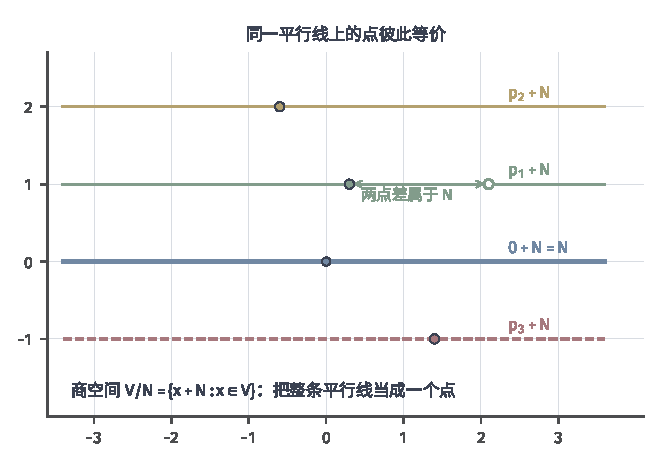
\includegraphics[width=112mm]{figures/01-mathematical-preliminaries-upper/03-linear-spaces/matplotlib/ls-quotient-equivalence-classes/ls-quotient-equivalence-classes.pdf}
  \caption{商空间的等价类。$V=\mathbb R^2$，子空间$U$为$x$轴（蓝线$0+U$）；每条平行直线$p+U=\{(x,p_y)\}$是一个等价类，图中画出$y=1$（绿）、$y=2$（黄）、$y=-1$（红虚线）。绿线上实点$(0.3,1)$与空心点$(2.1,1)$之差$(1.8,0)\in U$，故属同一类；商空间$V/U$把每条平行线当成一个点。}
  \label{fig:ls-quotient-equivalence-classes}
\end{figure}

这些类能否像向量一样相加和缩放？自然的做法是借代表元来算。
\begin{definition}[商空间]
\label{def:linear-algebra-quotient-space}
设$U$是线性空间$V$的子空间。全部等价类$\bm x+U$组成的集合记为$V/U$，规定
\[
 (\bm x+U)+(\bm y+U)=(\bm x+\bm y)+U,
 \qquad
 a(\bm x+U)=a\bm x+U,
\]
称$V/U$为$V$对$U$的\term{商空间}（quotient space）。
\end{definition}
借代表元定义运算，必须先检查结果与代表元的选取无关。换代表元$\bm x'=\bm x+\bm n_1$、$\bm y'=\bm y+\bm n_2$（$\bm n_1,\bm n_2\in U$）时，$\bm x'+\bm y'$与$\bm x+\bm y$只相差$\bm n_1+\bm n_2$，$a\bm x'$与$a\bm x$只相差$a\bm n_1$，二者都属于$U$，所以得到同一个类。零类是$U$本身，$\bm x+U$的相反类是$-\bm x+U$，其余规则由$V$的运算规则逐条继承，所以$V/U$构成线性空间。在图~\ref{fig:ls-quotient-equivalence-classes}中，两条水平线相加就是把高度相加：商空间只记录高度，被忽略的是沿$x$轴的位置。

回到截距的例子，商空间恰好只保留截距。
\begin{example}[只保留截距的商空间]
\label{ex:ls-quotient-intercept}
给定：$V=P_1=\{a+bt:a,b\in\mathbb R\}$与子空间$U=\{st:s\in\mathbb R\}$。

计算：$f_{a,b}=a+bt$所在的类是
\[
 f_{a,b}+U=\{a+(b+s)t:s\in\mathbb R\}=\{a+rt:r\in\mathbb R\},
\]
它只依赖$a$。两个类$f_{a,b}+U$与$f_{a',b'}+U$相等，当且仅当$f_{a,b}-f_{a',b'}=(a-a')+(b-b')t\in U$，即$a=a'$。按商空间的运算，
\[
 (f_{a,b}+U)+(f_{a',b'}+U)=f_{a+a',\,b+b'}+U,
 \qquad
 c(f_{a,b}+U)=f_{ca,\,cb}+U,
\]
即截距分别相加、缩放。

结论：规则$f_{a,b}+U\mapsto a$是从$P_1/U$到$\mathbb R$的双射，并保持加法与数乘。商空间$P_1/U$只记录截距，被忽略的是斜率。
\end{example}
商空间有多少个独立方向，要等下一节有了维数才能回答（第~\ref{sec:ls-dimension}节）；它与线性映射的联系在第~\ref{sec:ls-kernel-image}节给出。

% 第5章第2节：基、维数与坐标（线性无关与张成、基、维数、坐标与坐标变换）。

\section{基、维数与坐标}
\label{sec:ls-bases-dimension-coordinates}

上一节规定了在什么范围里作线性组合，但还没有回答怎样用有限个数记录一个对象。思路是选定一组方向，把对象写成它们的线性组合，用组合系数代替对象。这要求依次回答几个问题：一组方向能到达哪些对象；到达同一个对象的系数是否唯一；怎样挑出一组既够用又不重复的方向作为“尺子”；不同的尺子是否总含同样多根，即空间有多大；选定尺子以后，系数怎样代替对象参与计算，换一把尺子系数怎样换算。前一个问题的答案是后一个问题的前提，所以按这个顺序展开。

\subsection{线性无关与张成}

\paragraph{张成}
\phantomsection
\label{sec:ls-span}
在平面上，两个不共线方向的加权组合能取到每一个点；只有一个方向时，无论怎样加权，结果都停在过原点的一条直线上。要描述一组方向“能到达哪里”，先给它们的全部线性组合命名：给定$\bm v_1,\ldots,\bm v_k\in V$，集合
\begin{equation}
 \operatorname{span}\{\bm v_1,\ldots,\bm v_k\}
 =\left\{\sum_{j=1}^k a_j\bm v_j:a_j\in\mathbb R\right\}
 \label{eq:ls-span}
\end{equation}
称为这组向量的\term{张成空间}（span）。

两个线性组合再作线性组合，仍是这组向量的线性组合，所以张成空间对线性组合封闭，是$V$的子空间。任何包含$\bm v_1,\ldots,\bm v_k$的子空间都必须含有它们的全部线性组合，所以张成空间是包含这组向量的最小子空间。若$\operatorname{span}\{\bm v_1,\ldots,\bm v_k\}=V$，就说这组向量张成$V$，也称它们是$V$的一个生成组。

在$\mathbb R^m$中，把$\bm v_1,\ldots,\bm v_k$排成矩阵$\bm V$的各列，按列读法$\sum_ja_j\bm v_j=\bm V\bm a$，所以张成空间就是$\bm V$乘上全部系数向量所得的输出集合$\{\bm V\bm a:\bm a\in\mathbb R^k\}$，第~\ref{sec:ls-kernel-image}节将把它称为$\bm V$的列空间。如图~\ref{fig:ls-linear-combination-span}所示，两个不共线方向的组合取遍整个平面，单个方向的组合只是一条直线。
\begin{figure*}[htbp]
  \centering
  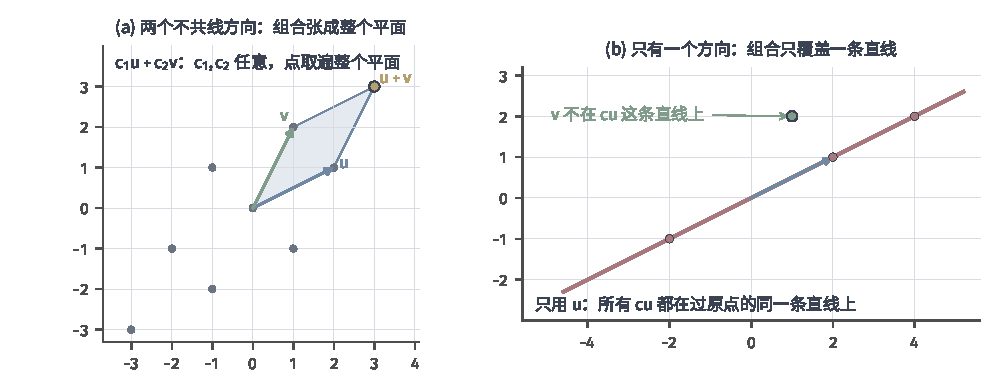
\includegraphics[width=169mm]{figures/01-mathematical-preliminaries-upper/03-linear-spaces/matplotlib/ls-linear-combination-span/ls-linear-combination-span.pdf}
  \caption{两个方向与一个方向的张成范围。左：$\bm u=(2,1)$（蓝箭头）与$\bm v=(1,2)$（绿箭头）的全部加权组合取遍整个平面，浅蓝平行四边形标出$0,\bm u,\bm u+\bm v,\bm v$，灰点为整数系数格点，黄点为$\bm u+\bm v=(3,3)$。右：只有$\bm u$一个方向时，组合$\{c\bm u\}$只是过原点的一条直线（红线），$\bm v$不在其上。两图坐标等比例，为解析教学例。}
  \label{fig:ls-linear-combination-span}
\end{figure*}

\paragraph{线性无关}
\phantomsection
\label{sec:ls-linear-dependence}
张成告诉我们哪些对象能被表示，却没有说明表示方式是否只有一种。若同一个对象可以用两组不同的系数写出，某些方向就是多余的。两组系数相减，就得到零向量的一个系数不全为零的表示，所以判断冗余，只需看零向量能否被非平凡地表示。若
\begin{equation}
 a_1\bm v_1+\cdots+a_k\bm v_k=\bm0
 \label{eq:linear-algebra-independence-relation}
\end{equation}
仅在全部$a_j=0$时成立，就称这组向量\term{线性无关}（linearly independent）；否则称为\term{线性相关}（linearly dependent），即存在不全为零的系数使式\eqref{eq:linear-algebra-independence-relation}成立。线性相关时挑出一个非零系数$a_j$并移项，就能把$\bm v_j$写成其余向量的线性组合，说明这个方向重复了已有方向能到达的范围。在$\mathbb R^m$中，线性无关就是齐次方程$\bm V\bm a=\bm0$只有零解；第~\ref{sec:ls-gram-orthogonality}节还将说明，它等价于Gram矩阵$\bm V^\top\bm V$正定。

贯穿例的两列几乎同向，它们是否线性无关？
\begin{example}[近共线的两列仍线性无关]
\label{ex:ls-nearly-collinear-independence}
给定：式~\eqref{eq:linear-algebra-nearly-collinear-design}中的$\bm c_1=(1,1,1)^\top$、$\bm q=(0,1,-1)^\top$与$\bm c_2=\bm c_1+\varepsilon\bm q$。

验证：先看$\bm c_1$与$\bm q$。$\alpha\bm c_1+\beta\bm q=(\alpha,\ \alpha+\beta,\ \alpha-\beta)^\top$为零时，第一坐标给出$\alpha=0$，第二坐标再给出$\beta=0$，所以$\bm c_1,\bm q$线性无关。再看两列：
\[
 a_1\bm c_1+a_2\bm c_2=(a_1+a_2)\bm c_1+a_2\varepsilon\bm q .
\]
它为零时，由$\bm c_1,\bm q$线性无关得$a_1+a_2=0$与$a_2\varepsilon=0$。

结论：$\varepsilon\neq0$时只能$a_2=0$，进而$a_1=0$，两列线性无关；$\varepsilon=0$时$\bm c_1-\bm c_2=\bm0$，两列线性相关。
\end{example}
所以“两列几乎同向”和线性无关是两回事。线性无关是精确的是非判断，只要$\varepsilon\neq0$就成立；几乎同向描述的是接近退化的程度，要由夹角或Gram矩阵衡量，第~\ref{sec:ls-inner-product-definition}节把这种情形称为近共线。

\paragraph{表示的存在与唯一}
“能表示哪些对象”和“表示是否冗余”是两个独立的问题，分别由张成与线性无关回答。下面的例子在平面上把二者分开。
\begin{example}[足够、不够与冗余的方向组]
\label{ex:ls-redundant-spanning-set}
给定：$\mathbb R^2$中的$\bm v_1=(1,0)^{\top}$、$\bm v_2=(0,1)^{\top}$与$\bm v_3=(1,1)^{\top}$。

计算：第一，$a_1\bm v_1+a_2\bm v_2=(a_1,a_2)^{\top}$，任一目标点$(x,y)^\top$都由唯一的系数$a_1=x$、$a_2=y$取到。第二，只取$\bm v_1$时，组合$a_1\bm v_1=(a_1,0)^\top$只能到达横轴，取不到$\bm v_2$。第三，取$\bm v_1,\bm v_2,\bm v_3$时，能到达的点仍是整个平面，但目标$(1,1)^\top$有两组系数：
\[
 0\bm v_1+0\bm v_2+1\bm v_3=(1,1)^\top=1\bm v_1+1\bm v_2+0\bm v_3 .
\]
两组系数相减，得到零向量的非平凡表示$\bm v_1+\bm v_2-\bm v_3=\bm0$。

结论：$(\bm v_1,\bm v_2)$足够且无冗余；$(\bm v_1)$不够；$(\bm v_1,\bm v_2,\bm v_3)$足够，但表示冗余。
\end{example}
图~\ref{fig:vol1-add-linear-redundant-directions}把第三种情形下的两种表示画到同一个平面上。
\begin{figure}[!htb]
  \centering
  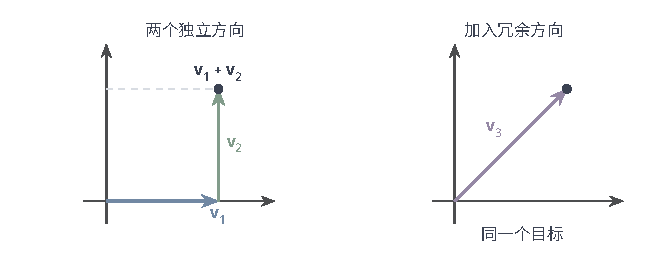
\includegraphics[width=112mm]{figures/01-mathematical-preliminaries-upper/03-linear-spaces/tikz/comprehension-additions/linear-redundant-directions.pdf}
  \caption{冗余方向与重复表示。取$\bm v_1=(1,0)^{\top}$、$\bm v_2=(0,1)^{\top}$与$\bm v_3=(1,1)^{\top}$。左图沿$\bm v_1$再沿$\bm v_2$，右图直接沿$\bm v_3$，到达同一个目标；前两向量已能表示平面中的每个向量，加入$\bm v_3$只使生成组冗余。两图坐标等比例。}
  \label{fig:vol1-add-linear-redundant-directions}
\end{figure}

这个例子中的现象是一般的。存在性来自张成：张成空间之内的对象必有一组系数。唯一性来自线性无关：若同一对象有两组系数，二者相减得到式\eqref{eq:linear-algebra-independence-relation}形式的关系，无关性迫使两组系数之差为零，即两组系数完全相同。

反过来，唯一性也蕴含无关性。若存在一组不全为零的系数使线性组合为零，把这组系数加到某个对象的一组表示上，就得到同一对象的第二组表示，表示不再唯一。所以“张成空间内每个对象的系数唯一”与“零向量只有平凡表示”是同一件事的两面，这正是后面定义坐标的根据。

\subsection{基}
\label{sec:ls-basis-dimension}

张成保证表示存在，无关保证表示唯一。同时满足张成和线性无关的一组向量称为\term{基}（basis）：它足够到达整个空间，又不重复，可以充当整个空间的一把“尺子”。

$\mathbb R^d$的标准坐标向量$\bm e_1,\ldots,\bm e_d$是一组基，称为标准基：$\bm x=\sum_jx_j\bm e_j$说明它们张成$\mathbb R^d$，而$\sum_ja_j\bm e_j=(a_1,\ldots,a_d)^\top=\bm0$迫使全部$a_j=0$。$P_k$中$1,t,\ldots,t^k$是一组基：每个多项式都是它们的组合，而组合为零多项式时各项系数都为零。

子空间也有基。下面为一个齐次方程的解集合求出一组基。
\begin{example}[齐次方程解平面的一组基]
\label{ex:ls-solution-plane-basis}
给定：$\mathbb R^3$中齐次方程$x_1+2x_2+3x_3=0$的解集合$N$；由示例~\ref{ex:ls-subspace-checks}，$N$是子空间。

计算：解满足$x_1=-2x_2-3x_3$，其中$x_2,x_3$可以任取，于是
\[
 \bm x=x_2(-2,1,0)^\top+x_3(-3,0,1)^\top .
\]
所以$\bm n_1=(-2,1,0)^\top$与$\bm n_2=(-3,0,1)^\top$张成$N$。若$a\bm n_1+b\bm n_2=(-2a-3b,\ a,\ b)^\top=\bm0$，比较第二、三个坐标得$a=b=0$，所以二者线性无关。

结论：$\bm n_1,\bm n_2$是$N$的一组基。
\end{example}

\paragraph{基的抽取与扩充}
若$V$有一个有限的生成组，就称$V$是有限维的；本章只讨论有限维空间。有限维空间总有基，而且可以从两个方向得到。

第一条路线是抽取。从任一有限生成组出发，若某个成员能写成其余向量的线性组合，删去它不会缩小张成范围。反复检查并删除，直到剩下的向量中没有一个能由其余向量表示。这时剩下的向量线性无关，又仍张成$V$，即构成一组基。

第二条路线是扩充。从任一线性无关组出发，逐次加入不在其张成空间中的向量。每加入一个新方向，张成范围严格扩大，新组仍线性无关：若新组的某个组合为零，新向量的系数必为零，否则新向量就能由原组表示，落在原张成空间中；新向量的系数为零以后，原组的无关性又使其余系数为零。下一小节的交换引理说明，有限维空间中线性无关组的长度不超过生成组的长度，所以扩充必在有限步内停止。停止时再也找不到张成空间之外的向量，留下的就是基。

两条路线互补：抽取把冗余的生成组压成基，扩充把线性无关组补成基。

\subsection{维数}
\label{sec:ls-dimension}

基的向量个数是空间大小的自然度量。但先要回答一个问题：换一组基，个数会不会变？答案由交换引理给出。
\begin{theorem}[交换引理]
\label{thm:ls-exchange-lemma}
若$\bm u_1,\ldots,\bm u_r$线性无关，且每个$\bm u_i$都属于$\operatorname{span}\{\bm v_1,\ldots,\bm v_s\}$，则$r\leq s$；并且这$r$个$\bm u_i$可以逐个换入原生成组、换出同样多个$\bm v_j$，每次换完新组仍张成原来的空间。
\end{theorem}
\begin{proof}
从生成组$G_0=\{\bm v_1,\ldots,\bm v_s\}$开始。因为$\bm u_1\in\operatorname{span}G_0$，它可写成若干$\bm v_j$的组合；这些系数不能全为零，否则$\bm u_1=\bm0$，与$\bm u_1,\ldots,\bm u_r$线性无关矛盾。取某个系数非零的$\bm v_j$，从这个表达式中把它解出来，$\bm v_j$就可由$\bm u_1$与其余$\bm v$的组合表示。于是用$\bm u_1$换出$\bm v_j$，新组$G_1$与$G_0$张成同一个空间。

一般地，设第$i-1$步后的组$G_{i-1}$由$\bm u_1,\ldots,\bm u_{i-1}$和$s-(i-1)$个幸存的$\bm v$组成，且与$G_0$张成同一空间。于是$\bm u_i\in\operatorname{span}G_{i-1}$。若$\bm u_i$只用$\bm u_1,\ldots,\bm u_{i-1}$就能表示，它与前面$i-1$个方向重复，违反线性无关；所以表达式中至少一个幸存$\bm v$的系数非零，把它解出并换入$\bm u_i$，张成范围不变。只要还有幸存的$\bm v$，这一步就能做下去。

若$r>s$，换满$s$次以后组内只剩$\bm u_1,\ldots,\bm u_s$，却仍有$\bm u_{s+1}$待入列；它属于$\operatorname{span}G_s=\operatorname{span}\{\bm u_1,\ldots,\bm u_s\}$，与$r$个$\bm u$线性无关矛盾。故$r\leq s$，而上面的逐次交换正是定理要求的换入换出过程。
\end{proof}

由此，基的个数与选取无关。任取两组基，设个数分别为$r$与$s$：把第一组看成无关组、第二组看成生成组，得$r\leq s$；互换两组的角色又得$s\leq r$，所以$r=s$。这个共同的个数称为空间的\term{维数}（dimension），记为$\dim V$。只含零向量的空间以空集为基，维数为$0$。

由上一小节的例子，$\dim\mathbb R^d=d$，$\dim P_k=k+1$；方程$x_1+2x_2+3x_3=0$的解集合维数为$2$（示例~\ref{ex:ls-solution-plane-basis}），过原点的直线$\{c\bm u:c\in\mathbb R\}$（$\bm u\neq\bm0$）维数为$1$。上一节“直线”“平面”的说法现在有了确切含义。交换引理的论证依赖有限的生成组，后面的基扩充与维数计算都在这一有限维范围内进行，不能直接搬到无限维的函数展开上。

\paragraph{子空间的维数}
有了维数，子空间之间可以比较大小。若$U\subseteq W$，取$U$的一组基，它在$W$中仍线性无关，可以按上一小节的扩充补成$W$的基。扩充只增加向量、不删去向量，因此$\dim U\leq\dim W$；新增方向的个数恰为$\dim W-\dim U$，记录$U$之外还有多少自由度。

包含且同维时，结论收紧为相等：$\dim U=\dim W$时，把$U$的基扩充成$W$的基不需要新增任何方向，它本身已经张成$W$，故$U=W$。这里的包含条件不能省略，同维本身推不出包含。
\begin{example}[反例：同维而互不包含的两条直线]
\label{ex:ls-equal-dimension-not-nested}
给定：$\mathbb R^2$中的$U=\{(s,0)^\top:s\in\mathbb R\}$与$W=\{(s,s)^\top:s\in\mathbb R\}$。

验证：$U$以$\bm e_1$为基，$W$以$(1,1)^\top$为基，所以$\dim U=\dim W=1$。但$\bm e_1\in U$的两个坐标不相等，不在$W$中；$(1,1)^\top\in W$的第二坐标不为零，也不在$U$中。

结论：两条直线维数相同，却互不包含。维数只数方向的个数，不管这些方向具体指向哪里。
\end{example}
后面的维数公式与秩零度定理，都复用这一“先取已有基、再补新方向”的做法。

\paragraph{和的维数公式}
和空间的维数不是两边维数的简单相加，因为公共方向会被重复计入。设$\bm z_1,\ldots,\bm z_k$是$U\cap W$的一组基，把它扩充为$U$的基$\bm z_1,\ldots,\bm z_k,\bm u_1,\ldots,\bm u_p$，再另行扩充为$W$的基$\bm z_1,\ldots,\bm z_k,\bm w_1,\ldots,\bm w_q$。下面说明这$k+p+q$个向量构成$U+W$的基。

它们张成$U+W$，因为每个$\bm u+\bm w$（$\bm u\in U$，$\bm w\in W$）都是两组基的组合。为证线性无关，设
\[
 \sum_i\alpha_i\bm z_i+\sum_j\beta_j\bm u_j+\sum_l\gamma_l\bm w_l=\bm0 .
\]
移项得$\sum_l\gamma_l\bm w_l=-\sum_i\alpha_i\bm z_i-\sum_j\beta_j\bm u_j$。左边属于$W$，右边属于$U$，所以这个向量属于$U\cap W$，可以写成$\sum_i\delta_i\bm z_i$。于是$\sum_l\gamma_l\bm w_l-\sum_i\delta_i\bm z_i=\bm0$，由$W$的基线性无关，全部$\gamma_l=0$。代回原式，再由$U$的基线性无关，全部$\alpha_i$与$\beta_j$也为零。因此$\dim(U+W)=k+p+q=(k+p)+(k+q)-k$，即
\begin{equation}
 \dim(U+W)=\dim U+\dim W-\dim(U\cap W).
 \label{eq:ls-dimension-formula}
\end{equation}
被减去的维数正是两边重复计入的公共方向，而不是两个集合元素个数的差。下面在$\mathbb R^3$中核对这一公式。
\begin{example}[两个坐标平面的和]
\label{ex:ls-dimension-formula-planes}
给定：$\mathbb R^3$中的$U=\operatorname{span}\{\bm e_1,\bm e_2\}$与$W=\operatorname{span}\{\bm e_2,\bm e_3\}$。

计算：$U$由第三坐标为零的向量组成，$W$由第一坐标为零的向量组成，所以$U\cap W$由第一、三坐标都为零的向量组成，即$U\cap W=\operatorname{span}\{\bm e_2\}$，维数为$1$。$U+W$含有$\bm e_1,\bm e_2,\bm e_3$，所以$U+W=\mathbb R^3$。代入公式：
\[
 \dim(U+W)=3=2+2-1 .
\]
若改取两条坐标轴$U'=\operatorname{span}\{\bm e_1\}$、$W'=\operatorname{span}\{\bm e_2\}$，交为零，$\dim(U'+W')=1+1-0=2$。

结论：公式中减去的$1$正是两个平面共有的$\bm e_2$方向；交为零时，和的维数等于两边维数之和。
\end{example}

\paragraph{补空间的存在}
第~\ref{sec:ls-direct-sum}节定义了补空间，现在可以说明它总存在。把$U$的基扩充为$V$的基，新增向量张成的子空间记为$W$。整组基张成$V$，所以$U+W=V$。若某向量同属$U$与$W$，它既是$U$的基向量的组合，又是新增向量的组合，两种写法相减，得到整组基的一个组合为零，系数只能全为零，所以$U\cap W=\{\bm0\}$。于是$V=U\oplus W$。由维数公式，直和时交的维数为零，$\dim V=\dim U+\dim W$。扩充的选择不唯一，补空间也就不唯一，这与平面中直线的例子一致。

\paragraph{商空间的维数}
同样的“先取已有基、再补新方向”也回答了第~\ref{sec:ls-quotient-spaces}节留下的问题：商空间$V/U$有多少个独立方向？取$U$的一组基$\bm u_1,\ldots,\bm u_s$并扩充为$V$的基$\bm u_1,\ldots,\bm u_s,\bm w_1,\ldots,\bm w_t$。新增向量的类$\bm w_1+U,\ldots,\bm w_t+U$张成$V/U$：任一$\bm x$写成整组基的组合，其中$U$部分落进零类被消去。这些类也线性无关：若$\sum_ja_j(\bm w_j+U)=U$，则$\sum_ja_j\bm w_j\in U$，它能由$\bm u_i$表示，整组基的线性无关性迫使全部$a_j=0$。因此
\begin{equation}
 \dim(V/U)=\dim V-\dim U.
 \label{eq:ls-quotient-dimension}
\end{equation}

商空间的维数恰好等于补空间的维数。新增方向$\bm w_j$张成$U$的一个补空间$W$，每个$\bm x$唯一分解为$\bm x=\bm u+\bm w$（$\bm u\in U$，$\bm w\in W$），于是类$\bm x+U=\bm w+U$中的点都形如$\bm w+\bm u'$（$\bm u'\in U$）。这样的点落在$W$中当且仅当$\bm u'\in U\cap W=\{\bm0\}$，所以每个类与$W$恰交于一点$\bm w$。选定补空间，就是为每个类选定一个代表元。补空间要选，商空间却不依赖任何选择，这是二者的区别。

示例~\ref{ex:ls-quotient-intercept}中，$\dim(P_1/U)=2-1=1$，商空间只剩截距这一个方向；图~\ref{fig:ls-quotient-equivalence-classes}中，$\dim(\mathbb R^2/U)=1$，只剩高度。

\subsection{坐标与坐标变换}
\label{sec:ls-coordinates}
\label{sec:linear-algebra-coordinates}

有了基，每个对象都有唯一的一组系数。怎样用这组系数代替对象参与计算？代替以后，系数的大小能否反映对象的大小？换一组基，系数怎样换算？本小节依次回答这三个问题。

\paragraph{有序基下的坐标}
固定有序基$\mathcal B=(\bm b_1,\ldots,\bm b_d)$后，对象$\bm v$唯一写成$\sum_{j=1}^d x_j\bm b_j$。系数列$[\bm v]_{\mathcal B}=(x_1,\ldots,x_d)^{\top}$称为$\bm v$在基$\mathcal B$下的\term{坐标}（coordinates）。

存在性来自张成，唯一性来自线性无关，所以坐标映射$\bm v\mapsto[\bm v]_{\mathcal B}$是从$V$到$\mathbb R^d$的双射：每个对象恰有一列坐标，每列实数$(x_1,\ldots,x_d)^{\top}$也恰好记录对象$\sum_jx_j\bm b_j$。它还保持线性组合：若$[\bm v]_{\mathcal B}=\bm x$、$[\bm w]_{\mathcal B}=\bm y$，则$a\bm v+b\bm w=\sum_j(ax_j+by_j)\bm b_j$，由唯一性得$[a\bm v+b\bm w]_{\mathcal B}=a\bm x+b\bm y$。因此对象上的线性运算可以完全交给坐标去算，算完再按基还原。

在$\mathbb R^d$中，把基向量排成矩阵$\bm B=[\bm b_1\ \cdots\ \bm b_d]$，按列读法$\bm v=\bm B[\bm v]_{\mathcal B}$，所以坐标就是方程$\bm B\bm x=\bm v$的唯一解。下面用这一方程求一个斜基下的坐标。
\begin{example}[同一向量在两组基下的坐标]
\label{ex:ls-coordinates-two-bases}
给定：$\mathbb R^2$中的向量$\bm x=(1,2)^\top$，标准基$(\bm e_1,\bm e_2)$，以及斜基$\mathcal B=(\bm b_1,\bm b_2)$，$\bm b_1=(2,1)^\top$、$\bm b_2=(-1,1)^\top$。

计算：标准基下$\bm x=1\cdot\bm e_1+2\cdot\bm e_2$，坐标为$(1,2)^\top$。斜基下的坐标$(c_1,c_2)^\top$满足$c_1\bm b_1+c_2\bm b_2=\bm x$，即
\[
 2c_1-c_2=1,\qquad c_1+c_2=2 .
\]
两式相加得$3c_1=3$，所以$c_1=1$、$c_2=1$。核对：$\bm b_1+\bm b_2=(1,2)^\top$。

结论：$[\bm x]_{\mathcal B}=(1,1)^\top$。向量本身没有移动，只是沿不同的基去量。
\end{example}
图~\ref{fig:ls-basis-coordinates}画出这两种读法。
\begin{figure*}[htbp]
  \centering
  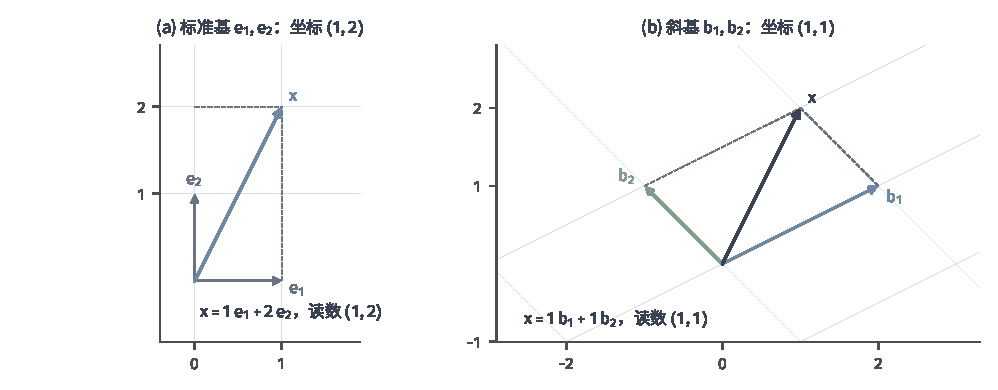
\includegraphics[width=169mm]{figures/01-mathematical-preliminaries-upper/03-linear-spaces/matplotlib/ls-basis-coordinates/ls-basis-coordinates.pdf}
  \caption{同一向量在两组基下的坐标。左：标准基$\bm e_1,\bm e_2$（灰箭头）下，向量$\bm x=(1,2)$（蓝箭头）的坐标为$(1,2)$，虚线为向坐标轴的垂线。右：斜基$\bm b_1=(2,1)$（蓝）、$\bm b_2=(-1,1)$（绿）下，同一个$\bm x$满足$\bm x=\bm b_1+\bm b_2$，坐标为$(1,1)$，浅色斜线为斜基网格，虚线为平行四边形读法。两图坐标系相同。}
  \label{fig:ls-basis-coordinates}
\end{figure*}

\paragraph{坐标与对象}
坐标列要与它所记录的对象区分开：几何位移、有限信号、多项式都可以相加和缩放，它们是\emph{对象}；一列实数只是选定基以后记录对象的\emph{坐标}。基的顺序也要固定：交换$\bm b_1,\bm b_2$，对象不变，坐标列的前两个数也随之交换。在$\mathbb R^d$中直接写数字列，通常是默认使用标准基$\bm e_1,\ldots,\bm e_d$，这时对象与坐标恰好是同一列数，第~\ref{chap:linear-operations}章正是在这种默认下工作的。

函数的基展开则必须区分二者：函数是对象，展开系数是坐标。
\begin{example}[仿射函数在两组基下的坐标]
\label{ex:ls-affine-function-coordinates}
给定：$P_1$中的$f_{a,b}=a+bt$，以及两组基$\mathcal B_1=(1,t)$与$\mathcal B_2=(1,1+t)$。

计算：在$\mathcal B_1$下$f_{a,b}=a\cdot1+b\cdot t$，坐标为$(a,b)^\top$。在$\mathcal B_2$下设$f_{a,b}=c_1\cdot1+c_2(1+t)=(c_1+c_2)+c_2t$，比较常数项与$t$的系数，得$c_2=b$、$c_1=a-b$，即
\[
 f_{a,b}=(a-b)\cdot1+b\cdot(1+t).
\]

结论：同一个函数在$\mathcal B_1$与$\mathcal B_2$下的坐标分别是$(a,b)^\top$与$(a-b,b)^\top$；坐标改变了，函数本身没有改变。
\end{example}
坐标的个数总是维数。一个对象若用冗余的生成组记录，记录的长度可以超过维数，所以不能由这种记录的长度推断空间有几维。

\paragraph{坐标对基的敏感性}
对象不变时，坐标仍可能相差很大。贯穿例给出一个数值上很极端的情形。
\begin{example}[近共线基下的大坐标]
\label{ex:ls-coordinate-instability}
给定：示例~\ref{ex:ls-nearly-collinear-independence}中的$\bm c_1,\bm q$与$\bm c_2=\bm c_1+\varepsilon\bm q$（$\varepsilon\neq0$），$\delta=0.1$，以及目标向量
\begin{equation}
 \bm y=\bm c_1+\delta\bm q=\begin{bmatrix}1\\1.1\\0.9\end{bmatrix}.
 \label{eq:linear-algebra-nearly-collinear-target}
\end{equation}
由该示例，$\mathcal B_0=(\bm c_1,\bm q)$与$\mathcal B_\varepsilon=(\bm c_1,\bm c_2)$都是平面$\operatorname{span}\{\bm c_1,\bm q\}$的基，$\bm y$也在这个平面中。

计算：在$\mathcal B_0$下，$\bm y$的坐标是$(1,\delta)^{\top}$。在$\mathcal B_\varepsilon$下，把$\bm q=(\bm c_2-\bm c_1)/\varepsilon$代入$\bm y=\bm c_1+\delta\bm q$，得
\begin{equation}
 \bm y=\left(1-\frac{\delta}{\varepsilon}\right)\bm c_1
       +\frac{\delta}{\varepsilon}\bm c_2.
 \label{eq:linear-algebra-coordinate-instability}
\end{equation}
取$\varepsilon=0.01$，则$\delta/\varepsilon=10$，坐标成为$(-9,10)^{\top}$。

结论：同一个$\bm y$在$\mathcal B_0$下的坐标为$(1,0.1)^\top$，在$\mathcal B_{0.01}$下的坐标为$(-9,10)^\top$。
\end{example}
两个很大的系数在几乎同向的两个基向量上相互抵消，不能据此判断原对象很大。这种系数对接近退化的基的敏感，将在第~\ref{chap:linear-analysis}章定量讨论。新旧坐标之间怎样系统地换算，是下面要回答的问题。

\paragraph{换基矩阵}
\phantomsection
\label{sec:ls-change-basis}
\label{sec:linear-algebra-coordinate-conversions}
设$\mathcal B=(\bm b_1,\ldots,\bm b_d)$与$\mathcal C$是$V$的两组有序基。已知$\bm v$在$\mathcal B$下的坐标$[\bm v]_{\mathcal B}=(x_1,\ldots,x_d)^{\top}$，怎样求它在$\mathcal C$下的坐标？由$\bm v=\sum_jx_j\bm b_j$，并且坐标映射保持线性组合，
\[
 [\bm v]_{\mathcal C}=\sum_{j=1}^d x_j[\bm b_j]_{\mathcal C}.
\]
右边是各列$[\bm b_j]_{\mathcal C}$以$x_j$为权重的线性组合。把这些列排成矩阵，称为从$\mathcal B$到$\mathcal C$的换基矩阵$\bm S_{\mathcal C\leftarrow\mathcal B}$，按矩阵与向量乘积的列读法，
\begin{equation}
 [\bm v]_{\mathcal C}
 =\bm S_{\mathcal C\leftarrow\mathcal B}[\bm v]_{\mathcal B}.
 \label{eq:linear-algebra-coordinate-change}
\end{equation}
换基矩阵的第$j$列是旧基向量$\bm b_j$的新坐标；下标$\mathcal C\leftarrow\mathcal B$从右向左读，表示把$\mathcal B$坐标译成$\mathcal C$坐标。下面在平面上算一个具体的换基矩阵。
\begin{example}[平面上的换基矩阵]
\label{ex:ls-change-of-basis-plane}
给定：$\mathbb R^2$的标准基$\mathcal E$与基$\mathcal U=(\bm u_1,\bm u_2)$，$\bm u_1=(1,0)^{\top}$、$\bm u_2=(1,1)^{\top}$；向量$\bm v$在$\mathcal U$下的坐标为$(1,1)^\top$。

计算：$\bm u_1,\bm u_2$的标准坐标就是它们自己。按“第$j$列是旧基向量的新坐标”，
\[
 \bm S_{\mathcal E\leftarrow\mathcal U}=\begin{bmatrix}1&1\\0&1\end{bmatrix}.
\]
由式~\eqref{eq:linear-algebra-coordinate-change}，$[\bm v]_{\mathcal E}=\bm S_{\mathcal E\leftarrow\mathcal U}(1,1)^{\top}=(2,1)^{\top}$。直接核对：$\bm v=\bm u_1+\bm u_2=(2,1)^\top$。

结论：$\mathcal U$坐标$(1,1)^\top$与标准坐标$(2,1)^\top$记录的是同一个向量。
\end{example}
图~\ref{fig:vol1-add-linear-change-basis}画出这一点：目标位置没有移动，改变的只是沿哪两条基方向累加，以及每条方向取多少份。
\begin{figure}[!htb]
  \centering
  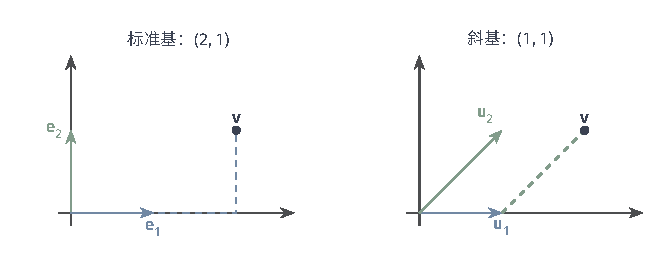
\includegraphics[width=112mm]{figures/01-mathematical-preliminaries-upper/03-linear-spaces/tikz/comprehension-additions/linear-change-basis.pdf}
  \caption{同一向量的两套坐标。左图使用标准基，$\bm v=(2,1)^{\top}$的坐标为$(2,1)^{\top}$；右图使用$\bm u_1=(1,0)^{\top}$、$\bm u_2=(1,1)^{\top}$，同一$\bm v$的坐标为$(1,1)^{\top}$。虚线表示相应的向量相加，两图的环境坐标比例相同。}
  \label{fig:vol1-add-linear-change-basis}
\end{figure}

\paragraph{连续换基与反向换基}
若再换到第三组基$\mathcal D$，中间那套坐标应当不留痕迹。对每个$\bm v$，连用两次式~\eqref{eq:linear-algebra-coordinate-change}，
\[
 [\bm v]_{\mathcal D}=\bm S_{\mathcal D\leftarrow\mathcal C}[\bm v]_{\mathcal C}=\bm S_{\mathcal D\leftarrow\mathcal C}\bm S_{\mathcal C\leftarrow\mathcal B}[\bm v]_{\mathcal B}.
\]
取$\bm v=\bm b_j$，它的$\mathcal B$坐标是$\bm e_j$，两边读出的分别是$\bm S_{\mathcal D\leftarrow\mathcal B}$与乘积的第$j$列，所以
\[
 \bm S_{\mathcal D\leftarrow\mathcal B}
 =\bm S_{\mathcal D\leftarrow\mathcal C}\bm S_{\mathcal C\leftarrow\mathcal B}.
\]

特别取$\mathcal D=\mathcal B$。每个$\bm b_j$在$\mathcal B$下的坐标是$\bm e_j$，所以左边$\bm S_{\mathcal B\leftarrow\mathcal B}=\bm I_d$，即$\bm S_{\mathcal B\leftarrow\mathcal C}\bm S_{\mathcal C\leftarrow\mathcal B}=\bm I_d$；交换两组基的角色，同理得$\bm S_{\mathcal C\leftarrow\mathcal B}\bm S_{\mathcal B\leftarrow\mathcal C}=\bm I_d$。所以换基矩阵总可逆，反向换基矩阵就是它的逆：$\bm S_{\mathcal B\leftarrow\mathcal C}=\bm S_{\mathcal C\leftarrow\mathcal B}^{-1}$。在示例~\ref{ex:ls-change-of-basis-plane}中，$\bm S_{\mathcal U\leftarrow\mathcal E}=\bm S_{\mathcal E\leftarrow\mathcal U}^{-1}=\left[\begin{smallmatrix}1&-1\\0&1\end{smallmatrix}\right]$，它把$(2,1)^{\top}$送回$(1,1)^{\top}$。

反过来，任一$d$阶可逆矩阵$\bm P$都是某次换基的矩阵。以$\bm P$的第$j$列为$\mathcal B$坐标，取向量$\bm b'_j=\sum_i\bm P_{i,j}\bm b_i$。$\bm P$的列线性无关，而坐标映射是保持线性组合的双射，所以$\bm b'_1,\ldots,\bm b'_d$也线性无关。个数等于维数的线性无关组必是基：否则它还能扩充，得到多于$\dim V$个线性无关的向量，与交换引理矛盾。于是$\bm b'_1,\ldots,\bm b'_d$构成一组基$\mathcal B'$。按定义，$\bm S_{\mathcal B\leftarrow\mathcal B'}$的第$j$列是$\bm b'_j$的$\mathcal B$坐标，即$\bm P$的第$j$列，所以$\bm S_{\mathcal B\leftarrow\mathcal B'}=\bm P$。

反向换基的代价取决于换基矩阵是否接近不可逆。贯穿例把这一点表现得很清楚。
\begin{example}[近共线基之间的换基]
\label{ex:ls-nearly-collinear-change-of-basis}
给定：示例~\ref{ex:ls-coordinate-instability}中的两组基$\mathcal B_0=(\bm c_1,\bm q)$与$\mathcal B_\varepsilon=(\bm c_1,\bm c_2)$，$\varepsilon\neq0$。

计算：由$\bm c_1=1\cdot\bm c_1+0\cdot\bm q$与$\bm c_2=1\cdot\bm c_1+\varepsilon\bm q$，$\mathcal B_\varepsilon$的两个向量在$\mathcal B_0$下的坐标分别是$(1,0)^{\top}$与$(1,\varepsilon)^{\top}$，所以
\[
 \bm S_{\mathcal B_0\leftarrow\mathcal B_\varepsilon}
 =\begin{bmatrix}1&1\\0&\varepsilon\end{bmatrix},
 \qquad
 \bm S_{\mathcal B_\varepsilon\leftarrow\mathcal B_0}
 =\bm S_{\mathcal B_0\leftarrow\mathcal B_\varepsilon}^{-1}
 =\begin{bmatrix}1&-1/\varepsilon\\0&1/\varepsilon\end{bmatrix},
\]
后者可由直接相乘验证。把$\bm y$在$\mathcal B_0$下的坐标$(1,\delta)^{\top}$代入后者，得
\[
 \bm S_{\mathcal B_\varepsilon\leftarrow\mathcal B_0}\begin{bmatrix}1\\\delta\end{bmatrix}
 =\begin{bmatrix}1-\delta/\varepsilon\\\delta/\varepsilon\end{bmatrix},
\]
与式~\eqref{eq:linear-algebra-coordinate-instability}一致。

结论：$\bm S_{\mathcal B_0\leftarrow\mathcal B_\varepsilon}$的行列式为$\varepsilon$，接近零；反向换基矩阵含有因子$1/\varepsilon$，小的基差异由此被放大成大系数。
\end{example}

\paragraph{被动换基与主动作用}
被动换基与主动作用必须分开。换基时对象不动、记录改变，式\eqref{eq:linear-algebra-coordinate-change}两侧是同一个$\bm v$的两套坐标；主动作用则在固定的坐标下把对象送到另一个对象，例如第~\ref{chap:linear-operations}章的矩阵作用$\bm x\mapsto\bm A\bm x$把向量旋转或切变，下一节把它推广为线性映射。两者都写成矩阵乘以坐标列，形式相似，含义不同。下面的例子在同一个初始向量上比较两种情形。
\begin{example}[被动换基与主动切变]
\label{ex:ls-passive-vs-active}
给定：$\mathbb R^2$中的向量$\bm x=(3,3)^\top$，斜基$\mathcal B'=(\bm b_1,\bm b_2)$，$\bm b_1=(2,1)^\top$、$\bm b_2=(-1,1)^\top$，以及切变矩阵$\bm A=\left[\begin{smallmatrix}1&1\\0&1\end{smallmatrix}\right]$。

计算：被动换基时，求$\bm x$在$\mathcal B'$下的坐标$(c_1,c_2)^\top$。由$2c_1-c_2=3$与$c_1+c_2=3$得$c_1=2$、$c_2=1$，即$\bm x=2\bm b_1+\bm b_2$。主动作用时，计算$\bm A\bm x=(3+3,\ 3)^\top=(6,3)^\top$。

结论：前者中向量仍是$(3,3)^\top$，只是读数从$(3,3)$变成$(2,1)$；后者中坐标系不动，向量本身被搬到$(6,3)^\top$。
\end{example}
图~\ref{fig:ls-passive-change-vs-active-map}把两种情形并排画出。所以不能把所有乘矩阵的运算都理解成换基。
\begin{figure*}[htbp]
  \centering
  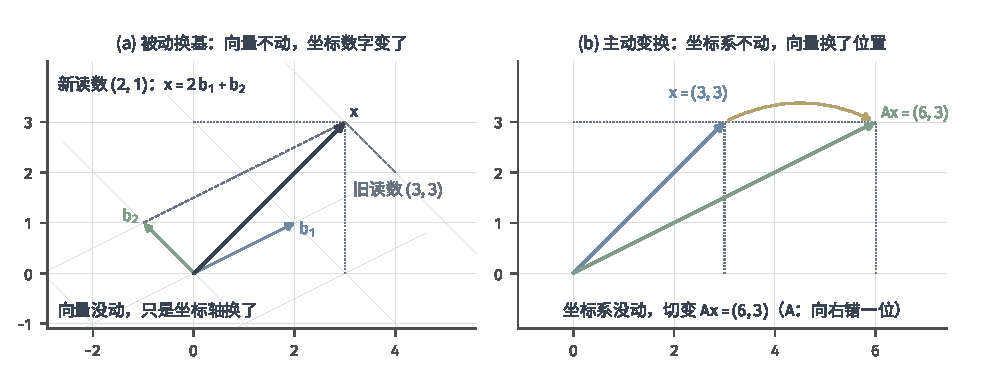
\includegraphics[width=169mm]{figures/01-mathematical-preliminaries-upper/03-linear-spaces/matplotlib/ls-passive-change-vs-active-map/ls-passive-change-vs-active-map.pdf}
  \caption{被动换基与主动变换的对照，两图使用同一个初始向量$\bm x=(3,3)$。左（被动换基）：箭头位置不动（深色），旧标准读数用点线投影读出$(3,3)$；新斜基$\bm b_1=(2,1)$（蓝）、$\bm b_2=(-1,1)$（绿）与浅色斜网格下，$\bm x=2\bm b_1+\bm b_2$，新读数为$(2,1)$。右（主动变换）：标准坐标系不动，$\bm x$（蓝）被切变映到$\bm A\bm x=(6,3)$（绿），黄色弧线表示搬动过程。}
  \label{fig:ls-passive-change-vs-active-map}
\end{figure*}

% 第5章第3节：线性映射（定义；表示：矩阵表示、基于矩阵的映射运算、矩阵基本子空间；核与像、秩零度、商空间、行空间与列空间、可逆性；换基：相抵与相似）。

\section{线性映射}
\label{sec:ls-linear-maps}
\label{sec:linear-algebra-matrices-linear-maps}

前两节研究的是单个空间中的对象怎样记录；本节转向对象之间的作用。一个作用要满足什么条件，才能用前两节的语言处理？选定基以后，它怎样记录成一张数表，两个作用叠加或接连进行时数表怎样变化？作用保留了哪些输入信息、丢失了哪些，什么时候可以由输出唯一反求输入？换一组基，记录同一个作用的数表怎样改变，哪些量不随之改变？本节的四个小节依次回答这四个问题。

\subsection{线性映射的定义}
\label{sec:ls-linear-map-definition}
\label{sec:linear-algebra-maps}

设计矩阵把一组系数变成一列拟合值，求导把一个多项式变成另一个多项式，读取第一个坐标把向量变成一个数。这些作用有一个共同点：输入先加权相加再作用，与先分别作用再作同样的加权相加，结果相同。正是这一点让前两节的语言可以用于作用本身：输入写成基向量的组合，作用就可以逐个基向量地计算。保持线性组合的作用称为\term{线性映射}（linear map）$T:V\to W$：
\begin{equation}
 T(a\bm x+b\bm y)=aT\bm x+bT\bm y,
 \qquad \bm x,\bm y\in V,\ a,b\in\mathbb R.
 \label{eq:ls-linear-map-def}
\end{equation}
取$a=b=0$得$T\bm0=\bm0$，线性映射总把原点留在原处。由式~\eqref{eq:prelim-matrix-linearity}，任何矩阵$\bm A\in\mathbb R^{m\times d}$给出的$\bm x\mapsto\bm A\bm x$都是从$\mathbb R^d$到$\mathbb R^m$的线性映射。下面再检查几个作用是否线性。
\begin{example}[线性与非线性的作用]
\label{ex:ls-linear-map-checks}
给定：三个作用
\[
 \begin{aligned}
 &T:\mathbb R^2\to\mathbb R^2, &&T(x_1,x_2)=(2x_1+x_2,\ 3x_2);\\
 &D:P_k\to P_k, &&Dp=p';\\
 &\tau:\mathbb R\to\mathbb R, &&\tau(x)=x+1.
 \end{aligned}
\]

验证：$T(x_1,x_2)$就是$\left[\begin{smallmatrix}2&1\\0&3\end{smallmatrix}\right]\bm x$，所以$T$保持线性组合。对多项式有$(ap+bq)'=ap'+bq'$，所以$D$保持线性组合；求导不升高次数，$D$确实把$P_k$送回$P_k$。$\tau(0)=1\neq0$，而线性映射必把$0$送到$0$。

结论：$T$与$D$是线性映射，$\tau$不是线性映射。
\end{example}

\phantomsection
\label{sec:ls-operator-powers}
输入与输出是同一个空间的线性映射$T:V\to V$称为\term{线性算子}（linear operator），也称线性变换。平面上的旋转、向一条直线的投影、$P_k$上的求导都是线性算子，示例~\ref{ex:ls-linear-map-checks}中的$T$也是。

算子是映射的特殊情形，但这一限制带来两点实质的不同。第一，输出仍在$V$中，可以再次作为输入，所以算子能与自身复合、反复作用：记$T^2=T\circ T$、$T^k=T\circ T^{k-1}$，并约定$T^0=\operatorname{id}_V$；一般映射$V\to W$在$V\neq W$时不能这样反复作用。下一小节将看到，在同一组基下，$T^k$的矩阵就是$T$的矩阵的$k$次幂。第二，记录算子时输入、输出可以用同一组基，这决定了算子换基时的特殊规律（第~\ref{sec:ls-similarity}节）。

\subsection{线性映射的表示（矩阵本质论）}
\label{sec:ls-map-representation}

线性映射的定义域通常有无穷多个元素，逐个记录输出是不可能的。本小节说明，有了基，有限个数就够了：在固定的两组基下，线性映射与矩阵一一对应，映射的叠加、复合与求逆分别对应矩阵的加法、乘法与求逆。第~\ref{chap:linear-operations}章的矩阵运算由此获得一般含义：矩阵就是线性映射在坐标下的记录。下面先建立这一对应，再把映射的运算翻译成矩阵的运算，最后对矩阵定义四个基本子空间，供下一小节计数信息的丢失与保留。

\subsubsection{矩阵表示}

给定输入基$\mathcal B=(\bm b_1,\ldots,\bm b_d)$，任一$\bm v=\sum_jx_j\bm b_j$的像由线性性写成
\[
 T\bm v=\sum_{j=1}^d x_j\,T\bm b_j,
\]
所以只要知道$d$个基向量的像，整个映射就确定了。再给定输出基$\mathcal C$，把每个像的坐标$[T\bm b_j]_{\mathcal C}$作为第$j$列，排成矩阵$\bm A=[T]_{\mathcal C\leftarrow\mathcal B}\in\mathbb R^{m\times d}$，称为$T$在这两组基下的矩阵。对上式两边取$\mathcal C$坐标，由坐标映射保持线性组合，并按矩阵与向量乘积的列读法，得到
\begin{equation}
 [T\bm v]_{\mathcal C}
 =\sum_{j=1}^d x_j\,[T\bm b_j]_{\mathcal C}
 =\sum_{j=1}^d x_j\bm A_{:,j}
 =[T]_{\mathcal C\leftarrow\mathcal B}\,[\bm v]_{\mathcal B}.
 \label{eq:linear-algebra-map-matrix-representation}
\end{equation}
也就是说，输出坐标等于矩阵乘以输入坐标：作用在对象上进行，记录在坐标上进行，二者由矩阵与向量的乘积连接。列数是输入维数，行数是输出维数；下标$\mathcal C\leftarrow\mathcal B$从右向左读，表示输入用$\mathcal B$记录、输出用$\mathcal C$记录。输入输出为同一空间的算子通常两端用同一组基，记为$[T]_{\mathcal B}=[T]_{\mathcal B\leftarrow\mathcal B}$，它是$\dim V$阶方阵。

下面按这一规则写出两个映射的矩阵。
\begin{example}[由基向量的像写出矩阵]
\label{ex:ls-plane-operator-matrix}
给定：示例~\ref{ex:ls-linear-map-checks}中的$T(x_1,x_2)=(2x_1+x_2,\ 3x_2)$，输入输出都取标准基。

计算：$T\bm e_1=(2,0)^{\top}$，$T\bm e_2=(1,3)^{\top}$。把它们依次作为两列，得
\[
 [T]=\begin{bmatrix}2&1\\0&3\end{bmatrix}.
\]

结论：$[T]$正是定义$T$时用的矩阵。
\end{example}
一般地，$\bm x\mapsto\bm A\bm x$在标准基下的矩阵就是$\bm A$本身，因为$\bm A\bm e_j=\bm A_{:,j}$。矩阵表示同样适用于不是数组的对象。
\begin{example}[求导的矩阵表示]
\label{ex:ls-derivative-matrix}
给定：求导$D:P_2\to P_2$，输入输出都取基$(1,t,t^2)$。

计算：$D1=0$，$Dt=1$，$Dt^2=2t$，三个像的坐标依次为$(0,0,0)^\top$、$(1,0,0)^\top$、$(0,2,0)^\top$，所以
\[
 [D]=\begin{bmatrix}0&1&0\\0&0&2\\0&0&0\end{bmatrix}.
\]
多项式$p=a_0+a_1t+a_2t^2$的坐标是$(a_0,a_1,a_2)^\top$，而$[D](a_0,a_1,a_2)^\top=(a_1,2a_2,0)^\top$，正是$p'=a_1+2a_2t$的坐标。

结论：对函数求导，在坐标下就是乘矩阵$[D]$。
\end{example}

\begin{theorem}[线性映射与矩阵的对应]
\label{thm:ls-map-matrix-correspondence}
设$\dim V=d$、$\dim W=m$，并固定$V$的基$\mathcal B$与$W$的基$\mathcal C$。则$T\mapsto[T]_{\mathcal C\leftarrow\mathcal B}$是从全部线性映射$V\to W$到全部$m\times d$实矩阵的双射。
\end{theorem}
\begin{proof}
单射：若两个线性映射的矩阵相同，它们在每个基向量上的像相同，由$T\bm v=\sum_jx_jT\bm b_j$，它们在每个$\bm v$上都相同。满射：任给$\bm A\in\mathbb R^{m\times d}$，对$\bm v\in V$令$T\bm v$为$\mathcal C$坐标等于$\bm A[\bm v]_{\mathcal B}$的那个向量。坐标唯一，所以这一规则有确定的意义；坐标映射与乘矩阵都保持线性组合，所以$T$线性；$T\bm b_j$的坐标是$\bm A\bm e_j=\bm A_{:,j}$，所以$[T]_{\mathcal C\leftarrow\mathcal B}=\bm A$。
\end{proof}
所以基固定以后，线性映射与矩阵一一对应；每个从$\mathbb R^d$到$\mathbb R^m$的线性映射在标准基下都等于乘某个矩阵。不过这一对应依赖基的选取：改变两端任一组基，通常会改变数表，而数表记录的仍是同一个映射。数表具体怎样随基改变，在第~\ref{sec:ls-coordinates-change-of-basis}节推导。

设计矩阵$\bm X_\varepsilon$正是这样一张记录：它表示$T_\varepsilon:\mathbb R^2\to\mathbb R^3$，$\bm w\mapsto\bm X_\varepsilon\bm w=w_1\bm c_1+w_2\bm c_2$，两列分别是两个输入基向量的像。输入是两个系数，输出是三个样本的拟合值，二者不能当成同一个空间中的向量。矩阵只是映射在两端坐标下的记录，不是映射本身的全部含义。图~\ref{fig:ch06-object-coordinate-map}中两条路径给出同一结果：先作用于对象再取坐标，与先取输入坐标再乘矩阵，得到相同的输出坐标。
\begin{figure}[htbp]
  \centering
  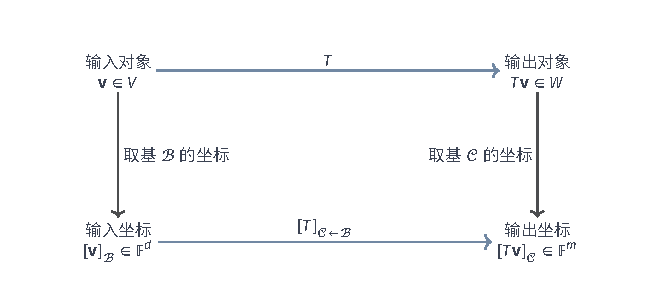
\includegraphics[width=112.0mm]{figures/01-mathematical-preliminaries-upper/03-linear-spaces/tikz/ch06-object-coordinate-map/figure.pdf}
  \caption{先作用于对象再取坐标，与先取输入坐标再按矩阵的列作线性组合（即乘矩阵），得到相同输出坐标。横向箭头改变对象或数值，竖向箭头只改变记录方式。}
  \label{fig:ch06-object-coordinate-map}
\end{figure}

\subsubsection{基于矩阵的映射运算}
\phantomsection
\label{sec:ls-map-addition-composition}

两个映射可以把输出相加，也可以接连作用；一个映射可能可以撤销，也可能带上常数偏置。第~\ref{chap:linear-operations}章的矩阵加法、乘法与求逆，正是前三种运算在固定基下的记录；带偏置的仿射映射则可以借增广坐标写成一张更大的矩阵。

\paragraph{叠加}
\phantomsection
\label{sec:linear-algebra-map-addition}
设$T,S:V\to W$是同一对空间之间的两个线性映射，定义
\[
 (aT+bS)(\bm x)=aT\bm x+bS\bm x,\qquad \bm x\in V,
\]
其中$a,b\in\mathbb R$。叠加保持线性：把输入的线性组合代入，两个分支分别展开再汇总即可。在$V$与$W$的固定基下，若$T,S$的矩阵为$\bm A,\bm B$，则$aT+bS$把第$j$个基向量送到$aT\bm b_j+bS\bm b_j$，其坐标是$a\bm A_{:,j}+b\bm B_{:,j}$，所以$aT+bS$的矩阵就是$a\bm A+b\bm B$。

相加的前提是两个映射的定义域与陪域都一致。这并不要求$V=W$：两个从$\mathbb R^2$到$\mathbb R^3$的映射照样可以相加，只是不能与一个从$\mathbb R^3$到$\mathbb R^2$的映射相加；这对应于只有同形矩阵才能相加。系数$a,b$必须与输入无关；若叠加系数随$\bm x$改变，叠加后的映射一般不再线性，需要单独检验。

\paragraph{复合}
设$T:U\to V$、$S:V\to W$是线性映射。复合$S\circ T$先$T$后$S$，仍保持线性组合：$S(T(a\bm x+b\bm y))=S(aT\bm x+bT\bm y)=aS(T\bm x)+bS(T\bm y)$。取$U,V,W$的基$\mathcal B,\mathcal C,\mathcal D$，对每个$\bm x\in U$，两次使用式~\eqref{eq:linear-algebra-map-matrix-representation}，再用矩阵乘法的结合律，得
\[
 [S(T\bm x)]_{\mathcal D}
 =[S]_{\mathcal D\leftarrow\mathcal C}[T\bm x]_{\mathcal C}
 =[S]_{\mathcal D\leftarrow\mathcal C}\bigl([T]_{\mathcal C\leftarrow\mathcal B}[\bm x]_{\mathcal B}\bigr)
 =\bigl([S]_{\mathcal D\leftarrow\mathcal C}[T]_{\mathcal C\leftarrow\mathcal B}\bigr)[\bm x]_{\mathcal B}.
\]
取$\bm x=\bm b_j$，其坐标是$\bm e_j$，两边读出的是$[S\circ T]_{\mathcal D\leftarrow\mathcal B}$与乘积的第$j$列，所以
\begin{equation}
 [S\circ T]_{\mathcal D\leftarrow\mathcal B}
 =[S]_{\mathcal D\leftarrow\mathcal C}\,[T]_{\mathcal C\leftarrow\mathcal B}.
 \label{eq:ls-composition-matrix}
\end{equation}

复合的矩阵是矩阵的乘积，中间空间$V$的基$\mathcal C$在乘积中被消去；第~\ref{sec:prelim-linear-actions-composition}节的推导是这里取标准基的特例。恒等映射$\operatorname{id}_V$在同一组基下的矩阵是单位矩阵。于是映射复合的结合律与矩阵乘法的结合律互相对应，矩阵乘法不可交换，也就是先后作用的次序不能交换。

对算子$T:V\to V$两端都用基$\mathcal B$，反复使用式~\eqref{eq:ls-composition-matrix}，得$[T^k]_{\mathcal B}=([T]_{\mathcal B})^k$：算子的反复作用记录为第~\ref{sec:ls-matrix-power-rules}节的矩阵幂。例如对示例~\ref{ex:ls-derivative-matrix}中的$[D]$直接相乘可得$[D]^3=\bm0$，这对应于任何次数不超过$2$的多项式求导三次都变为零。

\paragraph{逆映射}
第~\ref{sec:prelim-inverse-matrices}节把满足$\bm A\bm B=\bm B\bm A=\bm I$的方阵$\bm A$称为可逆矩阵，那里只把它看成一次可以撤销的数表运算。有了矩阵表示，就可以问它记录的是哪一类映射。若线性映射$T:V\to W$是双射（第~\ref{chap:sets-functions-and-proofs}章~\ref{sec:prelim-function-types}节），每个输出恰有一个原输入，逆映射$T^{-1}:W\to V$存在。逆映射自动是线性的：对$\bm w,\bm w'\in W$，由$T$的线性性
\[
 T\bigl(aT^{-1}\bm w+bT^{-1}\bm w'\bigr)=a\bm w+b\bm w',
\]
所以$aT^{-1}\bm w+bT^{-1}\bm w'$就是$a\bm w+b\bm w'$唯一的原输入，即$T^{-1}(a\bm w+b\bm w')=aT^{-1}\bm w+bT^{-1}\bm w'$。这样的$T$称为可逆线性映射。

可逆映射与可逆矩阵是同一件事的两种记录。设$T:V\to W$可逆，在基$\mathcal B,\mathcal C$下$\bm A=[T]_{\mathcal C\leftarrow\mathcal B}$，$\bm B=[T^{-1}]_{\mathcal B\leftarrow\mathcal C}$。由式~\eqref{eq:ls-composition-matrix}，$T^{-1}\circ T=\operatorname{id}_V$与$T\circ T^{-1}=\operatorname{id}_W$分别给出$\bm B\bm A=\bm I$与$\bm A\bm B=\bm I$，所以$\bm A$是可逆方阵（下一小节将说明此时必有$\dim V=\dim W$），且$[T^{-1}]_{\mathcal B\leftarrow\mathcal C}=\bm A^{-1}$。反过来，若$\bm A$可逆，$\bm y\mapsto\bm A^{-1}\bm y$就是$\bm x\mapsto\bm A\bm x$的逆映射。

两个可逆映射接连作用时，$(S\circ T)^{-1}=T^{-1}\circ S^{-1}$，在矩阵上就是式~\eqref{eq:ls-inverse-product}。至于一个映射什么时候可逆，要先弄清它丢失了什么、能到达什么，这是下一小节的内容。

\paragraph{仿射映射}
\phantomsection
\label{sec:ls-affine-maps}
线性模型的预测常带截距，平面上的平移也常与旋转一起出现，它们都不把原点留在原处。这样的作用怎样纳入线性映射的框架？带常数偏置的规则$\bm x\mapsto\bm A\bm x+\bm b$在$\bm b\neq\bm0$时称为\term{仿射映射}（affine map）。它不是线性映射：它把$\bm0$送到$\bm b$，而线性映射必将$\bm0$送到$\bm0$。两个仿射映射$\bm x\mapsto\bm A_1\bm x+\bm b_1$、$\bm y\mapsto\bm A_2\bm y+\bm b_2$复合得$\bm x\mapsto\bm A_2\bm A_1\bm x+(\bm A_2\bm b_1+\bm b_2)$，前一个映射的平移项也被后一个映射作用。

给坐标补一个恒为$1$的末位，仿射映射可以写成高一维空间上的线性作用：
\begin{equation}
 \begin{bmatrix}\bm A&\bm b\\ \bm0^\top&1\end{bmatrix}
 \begin{bmatrix}\bm x\\1\end{bmatrix}
 =
 \begin{bmatrix}\bm A\bm x+\bm b\\1\end{bmatrix}.
 \label{eq:ls-affine-homogeneous}
\end{equation}
按分块乘法，两个这样的增广矩阵相乘得
\[
 \begin{bmatrix}\bm A_2&\bm b_2\\ \bm0^\top&1\end{bmatrix}
 \begin{bmatrix}\bm A_1&\bm b_1\\ \bm0^\top&1\end{bmatrix}
 =\begin{bmatrix}\bm A_2\bm A_1&\bm A_2\bm b_1+\bm b_2\\ \bm0^\top&1\end{bmatrix},
\]
正是复合仿射映射的增广矩阵。

大矩阵对整个增广空间是线性的，但原输入被限制在末坐标为$1$的集合上，不能据此声称原映射线性。第~\ref{chap:linear-equations-and-optimization}章用这种形式描述仿射解集的几何。

\subsubsection{矩阵基本子空间}
\phantomsection
\label{sec:ls-four-fundamental-subspaces}

一张矩阵$\bm A\in\mathbb R^{m\times d}$既给出从$\mathbb R^d$到$\mathbb R^m$的映射$\bm x\mapsto\bm A\bm x$，它的转置$\bm A^\top\in\mathbb R^{d\times m}$又给出反方向的映射$\bm y\mapsto\bm A^\top\bm y$。对每个方向问两个问题：哪些输出可以到达，哪些输入被送到零。四个答案都是子空间，它们刻画了矩阵怎样保留和丢失信息。

按矩阵与向量乘积的列读法，$\bm A\bm x=\sum_jx_j\bm A_{:,j}$；$\bm x$取遍$\mathbb R^d$时，输出取遍$\bm A$各列的全部线性组合，即各列的张成空间，称为$\bm A$的\term{列空间}（column space），记为$\operatorname{range}(\bm A)$。所以方程$\bm A\bm x=\bm b$有解当且仅当$\bm b\in\operatorname{range}(\bm A)$。

齐次方程组$\bm A\bm x=\bm0$的解集合是$\mathbb R^d$的子空间（示例~\ref{ex:ls-subspace-checks}），称为$\bm A$的\term{零空间}（null space），记为$\operatorname{null}(\bm A)$。对$\bm A^\top$问同样的两个问题，又得到两个子空间。$\bm A^\top$的列就是$\bm A$的行（竖排），所以$\operatorname{range}(\bm A^\top)$由$\bm A$各行的线性组合组成，称为$\bm A$的\term{行空间}（row space）。$\bm A^\top\bm y=\bm0$转置后就是$\bm y^\top\bm A=\bm0^\top$：$\bm y^\top$从左边乘上$\bm A$得到零，所以$\operatorname{null}(\bm A^\top)$称为$\bm A$的\term{左零空间}（left null space）。这四个子空间合称$\bm A$的\term{四个基本子空间}（four fundamental subspaces）：
\begin{equation}
 \begin{aligned}
  \operatorname{range}(\bm A)&=\{\bm A\bm x:\bm x\in\mathbb R^d\}\subseteq\mathbb R^m,\\
  \operatorname{null}(\bm A)&=\{\bm x\in\mathbb R^d:\bm A\bm x=\bm0\}\subseteq\mathbb R^d,\\
  \operatorname{range}(\bm A^\top)&=\{\bm A^\top\bm y:\bm y\in\mathbb R^m\}\subseteq\mathbb R^d,\\
  \operatorname{null}(\bm A^\top)&=\{\bm y\in\mathbb R^m:\bm A^\top\bm y=\bm0\}\subseteq\mathbb R^m.
 \end{aligned}
 \label{eq:ls-four-fundamental-subspaces}
\end{equation}

零空间与行空间在输入空间$\mathbb R^d$中，列空间与左零空间在输出空间$\mathbb R^m$中。零空间收集被完全消去的输入方向。行空间收集读取输出分量所用的方向：输出的第$i$个分量$(\bm A\bm x)_i=\bm A_{i,:}\bm x$是第$i$行与$\bm x$逐项相乘再相加。左零空间收集对可达输出的“盲读”：对$\bm y\in\operatorname{null}(\bm A^\top)$与任意输入$\bm x$，$\bm y^\top(\bm A\bm x)=(\bm y^\top\bm A)\bm x=0$，即用$\bm y$对可达输出加权求和，结果总是零。

下面对一个具体矩阵求出四个基本子空间。
\begin{example}[一个$2\times3$矩阵的四个基本子空间]
\label{ex:ls-rank-one-four-subspaces}
给定：
\[
 \bm A=\begin{bmatrix}1&2&3\\2&4&6\end{bmatrix}\in\mathbb R^{2\times3}.
\]

计算：列空间：三列$(1,2)^\top$、$(2,4)^\top$、$(3,6)^\top$都是$(1,2)^\top$的倍数，所以$\operatorname{range}(\bm A)=\operatorname{span}\{(1,2)^\top\}$，是$\mathbb R^2$中的直线。零空间：第二行是第一行的$2$倍，$\bm A\bm x=\bm0$只剩一个方程$x_1+2x_2+3x_3=0$，由示例~\ref{ex:ls-solution-plane-basis}，$\operatorname{null}(\bm A)=\operatorname{span}\{(-2,1,0)^\top,(-3,0,1)^\top\}$，是$\mathbb R^3$中的平面。行空间：两行都是$(1,2,3)$的倍数，所以$\operatorname{range}(\bm A^\top)=\operatorname{span}\{(1,2,3)^\top\}$，是$\mathbb R^3$中的直线。左零空间：$\bm y^\top\bm A=(y_1+2y_2)(1,2,3)$为零当且仅当$y_1=-2y_2$，所以$\operatorname{null}(\bm A^\top)=\operatorname{span}\{(2,-1)^\top\}$，是$\mathbb R^2$中的直线。

结论：列空间、零空间、行空间、左零空间的维数依次为$1,2,1,1$。列空间与行空间维数相同；输入空间中零空间与行空间的维数之和为$2+1=3$，输出空间中列空间与左零空间的维数之和为$1+1=2$。此外，行空间的方向$(1,2,3)^\top$与零空间的两个基向量逐项相乘再相加都得零（$-2+2+0=0$，$-3+0+3=0$），列空间的方向$(1,2)^\top$与左零空间的方向$(2,-1)^\top$也是如此（$2-2=0$）。
\end{example}
第~\ref{sec:ls-kernel-image}节说明，示例中的两条维数规律对任何矩阵都成立；垂直关系则要等第~\ref{sec:ls-orthogonality}节有了内积以后才能说清。

\subsection{核与像}
\label{sec:ls-kernel-image}

一个映射丢失了哪些输入信息，又能产生哪些输出？这两个问题决定了能否由输出反求输入。本小节先把它们写成两个子空间，再用秩零度定理说明二者的维数此消彼长，并用商空间重新解读这一关系；然后求出矩阵四个基本子空间的维数；最后给出单射、满射与可逆的判据。

\paragraph{核与像}
被映射送到零的输入集合称为$T$的核（kernel），记为$\ker T=\{\bm x\in V:T\bm x=\bm0\}$；所有可到达的输出集合称为\term{像空间}（简称像，image），记为$\operatorname{im}T=\{T\bm x:\bm x\in V\}$。二者都是子空间：若$T\bm x=T\bm y=\bm0$，则$T(a\bm x+b\bm y)=\bm0$；若$\bm u=T\bm x$、$\bm v=T\bm y$，则$a\bm u+b\bm v=T(a\bm x+b\bm y)$。

核记录被映射完全消去的输入方向，像记录可达的输出范围；二者分别位于输入端与输出端，不能当作同一空间中的两个集合直接比较。对矩阵$\bm A\in\mathbb R^{m\times d}$，映射$\bm x\mapsto\bm A\bm x$的核就是零空间$\operatorname{null}(\bm A)$，像就是列空间$\operatorname{range}(\bm A)$（第~\ref{sec:ls-four-fundamental-subspaces}节）。说“矩阵$\bm A$的核”“矩阵$\bm A$的秩”时，指的都是映射$\bm x\mapsto\bm A\bm x$的相应量。

核为什么代表“丢失的信息”？因为$T\bm x=T\bm y$当且仅当$T(\bm x-\bm y)=\bm0$，即$\bm x-\bm y\in\ker T$：两个输入相差一个核方向时，输出完全相同。下面的例子用三个响应读取四个分量，展示这一点。
\begin{example}[相差核方向的输入给出相同输出]
\label{ex:ls-kernel-indistinguishable}
给定：$T:\mathbb R^4\to\mathbb R^3$，
\[
 T(x_1,x_2,x_3,x_4)=(x_1+x_4,\ x_2+x_4,\ x_3+x_4).
\]

计算：$T\bm x=\bm0$当且仅当$x_1=x_2=x_3=-x_4$，所以$\ker T=\operatorname{span}\{(1,1,1,-1)^{\top}\}$。取$x_4=0$时，$T\bm x=(x_1,x_2,x_3)$可以是任意向量，所以$\operatorname{im}T=\mathbb R^3$。两个输入$(1,1,1,1)^\top$与$(0,0,0,2)^\top$之差为$(1,1,1,-1)^\top\in\ker T$，相应地
\[
 T(1,1,1,1)=T(0,0,0,2)=(2,2,2).
\]

结论：仅凭三个响应无法区分这两个输入，也无法区分任何两个相差$(1,1,1,-1)^\top$倍数的输入。
\end{example}
这就是线性不可辨识性：两个输入相差核方向时输出相同，只凭输出无法确定输入。若另有约束限制了可取的输入，能否辨识还要结合这些约束判断。

\paragraph{秩零度定理}
\phantomsection
\label{sec:ls-rank-nullity}
核与像各有多大？二者的维数之间有一条精确的守恒关系。像的维数称为\term{秩}（rank）$\operatorname{rank}T=\dim\operatorname{im}T$，核的维数称为\term{零度}（nullity）$\dim\ker T$。
\begin{theorem}[秩零度定理]
\label{thm:ls-rank-nullity}
\label{thm:linear-algebra-rank-nullity}
有限维线性映射$T:V\to W$满足
\begin{equation}
 \dim V=\dim\ker T+\dim\operatorname{im}T,
 \qquad\text{即}\qquad
 \dim V=\dim\ker T+\operatorname{rank}T.
 \label{eq:ls-rank-nullity}
\end{equation}
\end{theorem}
\begin{proof}
取核的一组基$\bm v_1,\ldots,\bm v_r$并扩充成$V$的基$\bm v_1,\ldots,\bm v_d$。前$r$个基向量的像为零，所以其余像$T\bm v_{r+1},\ldots,T\bm v_d$张成像。若$\sum_{j>r}a_jT\bm v_j=\bm0$，则$\sum_{j>r}a_j\bm v_j$属于核，能由前$r$个基向量表示；整个基的线性无关性迫使全部$a_j=0$，所以这些像也是无关组。像的维数为$d-r$，结论成立。
\end{proof}
对矩阵$\bm A\in\mathbb R^{m\times d}$，记$\operatorname{rank}\bm A$为其映射的秩，即列空间的维数，有$d=\dim\operatorname{null}(\bm A)+\operatorname{rank}\bm A$。秩计数独立的输出方向，零度计数被消去的独立输入方向，二者此消彼长。在示例~\ref{ex:ls-kernel-indistinguishable}中，$\dim\ker T=1$、$\operatorname{rank}T=3$，二者之和为输入维数$4$。图~\ref{fig:ls-kernel-image-rank-nullity}再给出两个几何化算例：被映到零的方向与实际用到的输出方向，维数相加恰为定义域维数。
\begin{figure*}[htbp]
  \centering
  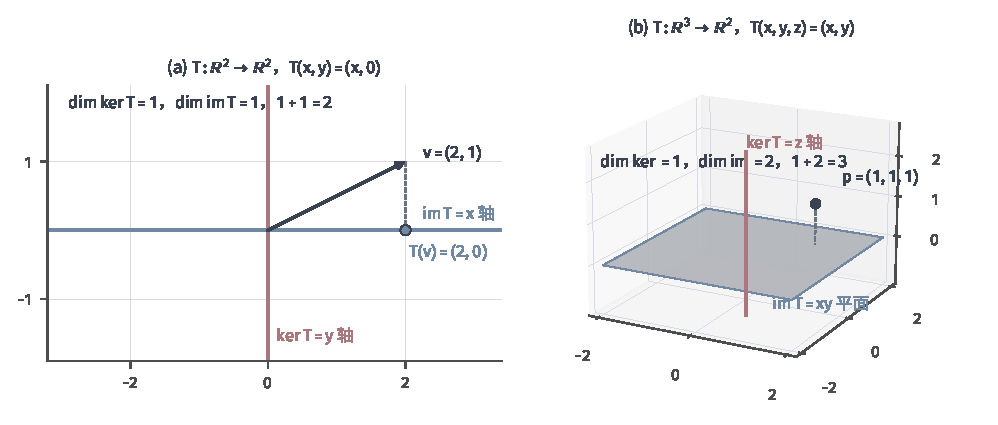
\includegraphics[width=169mm]{figures/01-mathematical-preliminaries-upper/03-linear-spaces/matplotlib/ls-kernel-image-rank-nullity/ls-kernel-image-rank-nullity.pdf}
  \caption{核与像的维数此消彼长。左：$T(x,y)=(x,0)$把平面映到$x$轴，核是$y$轴（红直线）、像是$x$轴（蓝直线），$\dim\ker T=1$、$\dim\operatorname{im}T=1$，$1+1=2$；样本$\bm v=(2,1)$被映到$(2,0)$。右：$T(x,y,z)=(x,y)$把三维空间映到$xy$平面，核是$z$轴（红直线）、像是整个$xy$平面（浅蓝），$\dim\ker T=1$、$\dim\operatorname{im}T=2$，$1+2=3$。两图为解析教学例。}
  \label{fig:ls-kernel-image-rank-nullity}
\end{figure*}

对$\bm A\in\mathbb R^{m\times d}$，$\operatorname{rank}\bm A\leq\min(m,d)$：列空间在$\mathbb R^m$中，维数不超过$m$；它由$d$列张成，从中抽取出的基不超过$d$个向量。$\operatorname{rank}\bm A=d$称为满列秩，这时输入方向全部被保留，等价于各列线性无关；$\operatorname{rank}\bm A=m$称为满行秩，这时输出全部可达；二者统称\term{满秩}（full rank）。

形状不同时，二者不能同时成立。$m<d$时，即使满行秩，核的维数也是$d-m>0$；$m>d$时，即使满列秩，像的维数也只有$d<m$，总有输出无法到达。例如贯穿例$\bm X_\varepsilon$在$\varepsilon\neq0$时两列线性无关（示例~\ref{ex:ls-nearly-collinear-independence}），秩为$2$，满列秩；它的像是$\mathbb R^3$中的一个平面，不是满行秩。

\paragraph{商空间}
前面看到，输出相同的输入恰好彼此相差一个核方向。按输出把输入分组，每组都形如$\bm x+\ker T$，正是第~\ref{sec:ls-quotient-spaces}节取$U=\ker T$得到的等价类，全部分组组成商空间$V/\ker T$。

规则$\bm x+\ker T\mapsto T\bm x$不依赖代表元，因为代表元相差核方向时输出相同。它保持线性组合，满射到$\operatorname{im}T$；它也是单射，因为两个类的像相同即$T\bm x=T\bm y$时，$\bm x-\bm y\in\ker T$，两个类相同。所以它是从$V/\ker T$到$\operatorname{im}T$的线性双射：压去全部丢失方向以后，每个等价类恰对应一个可达输出。线性双射把一组基送到一组基，两边维数相同；由式~\eqref{eq:ls-quotient-dimension}得$\dim V-\dim\ker T=\operatorname{rank}T$，这是秩零度定理的另一种读法。在示例~\ref{ex:ls-kernel-indistinguishable}中，商空间$\mathbb R^4/\ker T$是三维的，像$\mathbb R^3$也是三维的。

\paragraph{矩阵的行空间与列空间}
示例~\ref{ex:ls-rank-one-four-subspaces}中，行空间与列空间维数相同，零空间与行空间的维数之和为输入维数，列空间与左零空间的维数之和为输出维数。现在对一般的$\bm A\in\mathbb R^{m\times d}$证明这些规律。对$\bm A$用秩零度定理，零空间与列空间的维数之和为$d$；对$\bm A^\top$用它，左零空间与行空间的维数之和为$m$。剩下的问题是两个“列空间”之间的关系：行空间与列空间是否总一样大？
\begin{theorem}[行秩等于列秩]
\label{thm:ls-row-rank-column-rank}
对任意$\bm A\in\mathbb R^{m\times d}$，$\dim\operatorname{range}(\bm A^\top)=\dim\operatorname{range}(\bm A)$，即$\operatorname{rank}\bm A^\top=\operatorname{rank}\bm A$。
\end{theorem}
\begin{proof}
设$r=\operatorname{rank}\bm A$，取列空间的一组基$\bm c_1,\ldots,\bm c_r$，排成$\bm C\in\mathbb R^{m\times r}$。$\bm A$的每一列都在列空间中，所以第$j$列可写成$\bm A_{:,j}=\bm C\bm r_j$，$\bm r_j\in\mathbb R^r$；把这些系数列排成$\bm R\in\mathbb R^{r\times d}$，按乘积的列读法得$\bm A=\bm C\bm R$。再按行读这个乘积：$\bm A$的第$i$行是$\bm A_{i,:}=\sum_{k=1}^r\bm C_{i,k}\bm R_{k,:}$，即$\bm R$的$r$行的线性组合。所以$\bm A$的全部行都落在$\bm R$的$r$行张成的空间里，行空间的维数不超过$r$，即$\operatorname{rank}\bm A^\top\leq\operatorname{rank}\bm A$。对$\bm A^\top$用同样的论证，得$\operatorname{rank}\bm A\leq\operatorname{rank}\bm A^\top$，两者相等。
\end{proof}
于是行秩（行空间的维数）与列秩（列空间的维数）可以统称为秩。对$\bm A$与$\bm A^\top$分别用秩零度定理，四个基本子空间的维数全部由$m,d$与$r=\operatorname{rank}\bm A$决定：
\begin{equation}
 \begin{gathered}
 \dim\operatorname{range}(\bm A)=\dim\operatorname{range}(\bm A^\top)=r,\\
 \dim\operatorname{null}(\bm A)=d-r,\qquad
 \dim\operatorname{null}(\bm A^\top)=m-r.
 \end{gathered}
 \label{eq:ls-four-subspace-dimensions}
\end{equation}
输入空间中的零空间与行空间维数相加为$d$，输出空间中的列空间与左零空间维数相加为$m$。

对示例~\ref{ex:ls-rank-one-four-subspaces}中的$\bm A$，$r=1$，式~\eqref{eq:ls-four-subspace-dimensions}给出的维数与直接计算一致；证明中的分解$\bm A=\bm C\bm R$在那里就是$\bm A=(1,2)^\top(1,2,3)$。该示例还显示，两对子空间不仅维数互补，而且互相垂直。这一规律要在第~\ref{sec:ls-orthogonality}节有了内积以后才能说清；第~\ref{sec:ls-dual-map}节还将用对偶映射给出行秩等于列秩的另一个证明。

\paragraph{单射、满射与可逆性}
\phantomsection
\label{sec:ls-injective-surjective-invertible}
给定输出，能否唯一还原输入？这个问题分成两半：不同的输入是否给出不同的输出，以及每个输出是否都能被到达。对线性映射，这两半都可以用子空间判断。单射等价于核为零：$T\bm x=T\bm y$当且仅当$\bm x-\bm y\in\ker T$，核为零时输出相同必输入相同；反过来，核中若有非零向量，它与$\bm0$的输出相同，映射就不是单射。满射等价于像等于整个输出空间。有限维时可以用秩零度定理把二者换成维数：单射当且仅当$\operatorname{rank}T=\dim V$，满射当且仅当$\operatorname{rank}T=\dim W$。

输入输出维数相等时，秩零度定理使三种性质合而为一：$\dim V=\dim W$时，$\ker T=\{\bm0\}$等价于$\operatorname{rank}T=\dim V=\dim W$，于是单射、满射、双射互相等价，只需检查其中一条。维数不同时则须分别判断：$\dim V<\dim W$时像的维数至多为$\dim V$，不可能满射；$\dim V>\dim W$时核的维数至少为$\dim V-\dim W>0$，不可能单射。所以只有输入输出维数相等的映射才可能双侧可逆，矩形矩阵即使满秩，也只能是单射或满射之一。

把这些判据与上一小节可逆映射和逆矩阵的对应合起来，对$n$阶方阵$\bm A$，下列条件互相等价：
\[
 \bm A\text{可逆}
 \iff\operatorname{null}(\bm A)=\{\bm0\}
 \iff\operatorname{rank}\bm A=n
 \iff\bm A\text{的}n\text{列线性无关}.
\]
其中第三、四个条件等价，是因为列空间由$n$列张成，维数为$n$恰好说明这$n$列构成它的一组基。由行秩等于列秩，还可以在链中加入“$\bm A$的$n$行线性无关”。第~\ref{sec:ls-determinant-invertibility}节讨论线性方程时，还将用行列式给出一个等价的数值判据$\det\bm A\neq0$。

这一等价还给出第~\ref{sec:ls-square-one-sided-inverse}节“方阵的单侧逆即逆”的另一个证明，不必借助行列式。若$n$阶方阵满足$\bm B\bm A=\bm I_n$，则$\bm A\bm x=\bm0$蕴含$\bm x=\bm B\bm A\bm x=\bm0$，核为零，$\bm A$可逆，于是$\bm B=\bm B\bm A\bm A^{-1}=\bm A^{-1}$；$\bm A\bm B=\bm I_n$时对$\bm B$作同样论证。

同理，若$n$阶方阵的乘积$\bm A\bm B$可逆，则两个因子都可逆。$\bm B\bm x=\bm0$蕴含$\bm A\bm B\bm x=\bm0$，从而$\bm x=\bm0$，$\bm B$的核为零，因而可逆；于是$\bm A=(\bm A\bm B)\bm B^{-1}$是可逆矩阵的乘积，也可逆。

最容易还原的情形是逐坐标缩放；一般的矩阵把坐标掺在一起，但判据相同：核为零且维数相等。
\begin{example}[用核判断可逆]
\label{ex:ls-kernel-invertibility}
给定：对角矩阵$\operatorname{diag}(d_1,\ldots,d_n)$与$\bm A=\left[\begin{smallmatrix}2&1\\0&3\end{smallmatrix}\right]$。

验证：对角矩阵逐坐标缩放，坐标之间互不影响。若每个$d_i\neq0$，逐坐标除以$d_i$即可撤销，逆矩阵为$\operatorname{diag}(1/d_1,\ldots,1/d_n)$。若某个$d_i=0$，相应坐标被压为零，$\bm e_i$落入核中，两个只在第$i$个坐标不同的输入给出相同输出。对$\bm A$，$\bm A\bm x=\bm0$即$2x_1+x_2=0$与$3x_2=0$；第二式给出$x_2=0$，代入第一式得$x_1=0$，所以核为零。

结论：对角矩阵可逆当且仅当全部$d_i\neq0$；$\bm A$是方阵且核为零，所以可逆，它的逆矩阵已在第~\ref{sec:prelim-inverse-matrices}节求出。
\end{example}

\paragraph{单侧逆}
维数不同时，仍可以只撤销一半。单射$T:V\to W$可以找到线性映射$L:W\to V$使$L\circ T=\operatorname{id}_V$：在像上按$T$的逆读回输入，在像的一个补空间上任意规定（例如送到零）。满射$T$可以找到$R:W\to V$使$T\circ R=\operatorname{id}_W$：为输出基中的每个向量任选一个原输入，再线性延拓。补空间与原输入的选法不唯一，所以这些单侧逆一般也不唯一。

写成矩阵，对$\bm A\in\mathbb R^{m\times d}$：$\bm A$有左逆当且仅当它满列秩，有右逆当且仅当它满行秩。充分性来自上面的构造，因为满列秩就是单射，满行秩就是满射。必要性同样直接：若$\bm L\bm A=\bm I_d$，则$\bm A\bm x=\bm0$蕴含$\bm x=\bm L\bm A\bm x=\bm0$，核为零；若$\bm A\bm R=\bm I_m$，则每个$\bm y=\bm A(\bm R\bm y)$都可到达。第~\ref{sec:prelim-inverse-matrices}节的例子$\bm A=(1,0)^\top$满列秩，有无穷多个左逆。多解时如何选择代表，由第~\ref{chap:linear-equations-and-optimization}章回答。

\subsection{线性映射的换基}
\label{sec:ls-coordinates-change-of-basis}

第~\ref{sec:ls-coordinates}节看到，同一个对象在不同基下有不同的坐标；同样，同一个线性映射换一组基，记录它的矩阵通常也随之改变。现在坐标变换、矩阵表示与逆矩阵都已齐备，这种变化可以精确写出。本小节回答两个问题：一般线性映射在输入、输出两端各自换基以后，矩阵怎样变化，两个同形矩阵什么时候记录同一个映射；线性算子两端一起换基时，又会怎样。

一般映射放在算子之前。映射的两端是两个空间，可以独立换基，得到的关系称为相抵；算子要求两端使用同一组基，换基时两端必须一起变，相应的关系称为相似，它是相抵加上“两端换基相同”这一约束的特例。约束减少了可用的自由度：相抵只需秩就能完全分类，相似却要更多不变量。

推导要用到一个观察：换基矩阵本身就是一个线性映射的矩阵。比较式~\eqref{eq:linear-algebra-coordinate-change}与式~\eqref{eq:linear-algebra-map-matrix-representation}可见，$\bm S_{\mathcal C\leftarrow\mathcal B}$正是恒等映射$\operatorname{id}_V$在输入基$\mathcal B$、输出基$\mathcal C$下的矩阵：对象不动，只是输入端与输出端用不同的基记录。连续换基的乘法公式，也就是复合公式~\eqref{eq:ls-composition-matrix}对$\operatorname{id}_V\circ\operatorname{id}_V=\operatorname{id}_V$的特例。

\subsubsection{一般线性映射的换基与相抵}
\label{sec:ls-equivalence-matrices}

设$T:V\to W$是线性映射，$\dim V=d$、$\dim W=m$。它在一对基下记录为矩阵$\bm A$，在另一对基下记录为$\bm B$，$\bm A$与$\bm B$有什么关系？反过来，两个同形矩阵什么时候记录的是同一个映射？

\paragraph{换基过程}
设$\mathcal B,\mathcal B'$是$V$的两组基，$\mathcal C,\mathcal C'$是$W$的两组基，记$\bm A=[T]_{\mathcal C\leftarrow\mathcal B}$、$\bm B=[T]_{\mathcal C'\leftarrow\mathcal B'}$，输入端换基矩阵$\bm P=\bm S_{\mathcal B\leftarrow\mathcal B'}$（$d$阶可逆），输出端换基矩阵$\bm Q=\bm S_{\mathcal C\leftarrow\mathcal C'}$（$m$阶可逆）。$\bm P$的第$j$列是新输入基向量在旧输入基下的坐标，$\bm Q$同理。已知新输入坐标$[\bm v]_{\mathcal B'}$，求新输出坐标$[T\bm v]_{\mathcal C'}$，可以绕道旧基分三步完成。

第一步，把新输入坐标换成旧输入坐标：$[\bm v]_{\mathcal B}=\bm P[\bm v]_{\mathcal B'}$。第二步，在旧基下作用：$[T\bm v]_{\mathcal C}=\bm A[\bm v]_{\mathcal B}=\bm A\bm P[\bm v]_{\mathcal B'}$。第三步，把旧输出坐标换成新输出坐标，这要用反向换基矩阵$\bm Q^{-1}=\bm S_{\mathcal C'\leftarrow\mathcal C}$：
\[
 [T\bm v]_{\mathcal C'}=\bm Q^{-1}[T\bm v]_{\mathcal C}=\bm Q^{-1}\bm A\bm P[\bm v]_{\mathcal B'}.
\]
另一方面，按定义$[T\bm v]_{\mathcal C'}=\bm B[\bm v]_{\mathcal B'}$。两式对每个$\bm v$成立；取$\bm v=\bm b'_j$，其新坐标为$\bm e_j$，两边读出的是两个矩阵的第$j$列，所以
\begin{equation}
 \bm B=\bm Q^{-1}\bm A\bm P.
 \label{eq:ls-equivalence-transform}
\end{equation}
从右向左读：$\bm P$把新输入坐标译成旧坐标，$\bm A$在旧基下作用，$\bm Q^{-1}$把结果译成新输出坐标。用复合的语言说，$T=\operatorname{id}_W\circ T\circ\operatorname{id}_V$，三个因子分别在相应的基下记录，由式~\eqref{eq:ls-composition-matrix}就是上式右端的三个矩阵。

\paragraph{相抵的定义}
\phantomsection
\label{sec:ls-equivalence-meaning}
上面的推导说明，同一映射的两个记录之间只相差两侧各乘一个可逆矩阵。反过来，两侧任意乘上可逆矩阵，得到的是否仍是同一映射的记录？先把这种关系单独命名。
\begin{definition}[矩阵相抵]
\label{def:ls-matrix-equivalence}
设$\bm A,\bm B\in\mathbb R^{m\times d}$。若存在可逆矩阵$\bm Q\in\mathbb R^{m\times m}$与$\bm P\in\mathbb R^{d\times d}$使$\bm B=\bm Q^{-1}\bm A\bm P$，就称$\bm A$与$\bm B$\term{相抵}（equivalent matrices）。
\end{definition}
定义中的$\bm Q,\bm P$可以是任意可逆矩阵，不必事先知道它们来自哪组基；写成$\bm Q^{-1}$只是为了与换基推导一致，$\bm Q$取遍全部可逆矩阵时$\bm Q^{-1}$也取遍全部可逆矩阵。

相抵恰好刻画“记录同一个映射”。一个方向已由换基推导给出。另一方向，设$\bm A=[T]_{\mathcal C\leftarrow\mathcal B}$，任给可逆的$\bm P,\bm Q$。由第~\ref{sec:ls-coordinates}节，以$\bm P$的各列为旧基坐标可以得到$V$的一组新基$\mathcal B'$，使$\bm S_{\mathcal B\leftarrow\mathcal B'}=\bm P$；输出端用$\bm Q$同样构造$\mathcal C'$。由换基推导，$T$在这两组新基下的矩阵恰为$\bm Q^{-1}\bm A\bm P$。所以两个同形矩阵相抵，当且仅当它们是同一个线性映射在两端不同选基下的记录。右乘$\bm P$对应输入基的更换，左乘$\bm Q^{-1}$对应输出基的更换；初等列变换与初等行变换分别是这两种换基的具体实现。

\paragraph{相抵不变量}
\phantomsection
\label{sec:ls-equivalence-properties}
既然相抵的矩阵记录同一个映射，映射本身的性质就不应随基改变。哪些量是这样的不变量？相抵首先是等价关系：自反取$\bm Q=\bm P=\bm I$；对称由$\bm A=\bm Q\bm B\bm P^{-1}=(\bm Q^{-1})^{-1}\bm B\bm P^{-1}$；传递由$\bm C=\bm Q_2^{-1}\bm B\bm P_2=(\bm Q_1\bm Q_2)^{-1}\bm A(\bm P_1\bm P_2)$。三条分别对应不换基、换回原基和连续换两次基。

零空间在输入端被搬运：$\bm B\bm x=\bm0$当且仅当$\bm A(\bm P\bm x)=\bm0$，所以$\operatorname{null}(\bm B)=\bm P^{-1}\operatorname{null}(\bm A)$。列空间在输出端被搬运：$\bm B\bm x=\bm Q^{-1}\bm A(\bm P\bm x)$，而$\bm P\bm x$取遍全部输入，所以$\operatorname{range}(\bm B)=\bm Q^{-1}\operatorname{range}(\bm A)$。可逆矩阵把线性无关组送到线性无关组，搬运不改变子空间的维数，因此
\begin{equation}
 \operatorname{rank}\bm B=\operatorname{rank}\bm A,
 \qquad
 \dim\operatorname{null}(\bm B)=\dim\operatorname{null}(\bm A)=d-\operatorname{rank}\bm A.
 \label{eq:ls-equivalence-invariants}
\end{equation}
相抵允许的记录变化很宽：输入与输出可以是不同空间，$\bm B$一般不是方阵，不能对自身反复作用，所以幂、迹这类只对算子有意义的量不在讨论之列。

\paragraph{秩标准形与相抵判据}
\phantomsection
\label{sec:ls-equivalence-conditions}
秩是相抵不变量；反过来，秩相同的两个同形矩阵是否一定相抵？答案是肯定的。办法是说明两端可以独立选基时，每个矩阵都能化成只由秩决定的简单形状。设$\bm A$是$T$在某对基下的矩阵，$r=\operatorname{rank}\bm A$。取$\ker T$的一组基并扩充为$V$的基，由秩零度定理，新增向量恰有$r$个，把它们排在前面。这$r$个向量的像线性无关：若像的某个组合为零，相应的新增向量组合就落进核，能由核的基表示，整组基的线性无关性迫使系数全为零。核的基向量的像都是零，所以这$r$个像还张成$\operatorname{im}T$。再把这$r$个像扩充为$W$的基。在这样选取的两组基下，$T$把前$r$个输入基向量依次送到前$r$个输出基向量，其余输入基向量送到零，矩阵为秩标准形
\begin{equation}
 \begin{bmatrix}\bm I_r&\bm0\\\bm0&\bm0\end{bmatrix},
 \qquad r=\operatorname{rank}\bm A.
 \label{eq:ls-rank-normal-form}
\end{equation}

下面对一个秩为$1$的二阶矩阵具体做出这两组基。
\begin{example}[两端各自选基化为秩标准形]
\label{ex:ls-rank-normal-form-two-by-two}
给定：$\bm A=\left[\begin{smallmatrix}1&2\\2&4\end{smallmatrix}\right]$，$T\bm x=\bm A\bm x$，两端原来都用标准基。

计算：两列共线，$\operatorname{rank}\bm A=1$；$\bm A(-2,1)^\top=\bm0$，所以$\ker T=\operatorname{span}\{(-2,1)^\top\}$。输入端取$\bm v_1=\bm e_1$与核中的$\bm v_2=(-2,1)^{\top}$，输出端取$\bm w_1=\bm A\bm v_1=(1,2)^{\top}$并补上$\bm w_2=\bm e_2$。以新基向量的标准坐标为列，
\[
 \bm P=\begin{bmatrix}1&-2\\0&1\end{bmatrix},\qquad
 \bm Q=\begin{bmatrix}1&0\\2&1\end{bmatrix},\qquad
 \bm Q^{-1}=\begin{bmatrix}1&0\\-2&1\end{bmatrix}.
\]
先算$\bm A\bm P=\left[\begin{smallmatrix}1&0\\2&0\end{smallmatrix}\right]$，再左乘$\bm Q^{-1}$：
\[
 \bm Q^{-1}\bm A\bm P=\begin{bmatrix}1&0\\-2&1\end{bmatrix}\begin{bmatrix}1&0\\2&0\end{bmatrix}
 =\begin{bmatrix}1&0\\0&0\end{bmatrix}.
\]

结论：在新基下，$T$把$\bm v_1$送到$\bm w_1$，把核方向$\bm v_2$送到零，矩阵为秩标准形$\operatorname{diag}(1,0)$。
\end{example}
图~\ref{fig:ls-equivalence-two-sided-bases-flow}画出这两组基：$\bm v_1$被送到$\bm w_1$，核方向$\bm v_2$被送到零，输出端的$\bm w_2$不被任何输入到达。两端各自选基，才能同时做到这两件事；若要求两端用同一组基，这一化简一般做不到。
\begin{figure}[!htb]
  \centering
  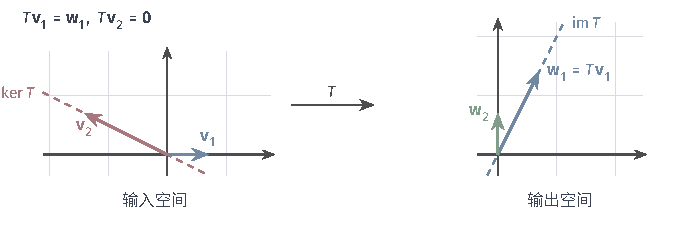
\includegraphics[width=112mm]{figures/01-mathematical-preliminaries-upper/03-linear-spaces/tikz/comprehension-additions/equivalence-two-bases.pdf}
  \caption{两端独立选基化为秩标准形。$T(\bm x)=\bm A\bm x$，$\bm A=\left[\begin{smallmatrix}1&2\\2&4\end{smallmatrix}\right]$。左：输入基$\bm v_1=\bm e_1$（蓝）与$\bm v_2=(-2,1)^{\top}$（红），$\bm v_2$在核（红虚线）上。右：输出基$\bm w_1=T\bm v_1=(1,2)^{\top}$（蓝）位于像（蓝虚线）上，$\bm w_2=\bm e_2$（绿）补足一组基。在这两组基下$T$的矩阵为$\operatorname{diag}(1,0)$。}
  \label{fig:ls-equivalence-two-sided-bases-flow}
\end{figure}

\begin{theorem}[相抵判据]
\label{thm:ls-equivalence-criterion}
两个同形实矩阵$\bm A,\bm B\in\mathbb R^{m\times d}$相抵，当且仅当$\operatorname{rank}\bm A=\operatorname{rank}\bm B$。
\end{theorem}
\begin{proof}
必要性由式\eqref{eq:ls-equivalence-invariants}得到。充分性：设二者秩都为$r$，由上面的构造，存在可逆矩阵使$\bm R=\bm Q_A^{-1}\bm A\bm P_A=\bm Q_B^{-1}\bm B\bm P_B$，其中$\bm R$是式\eqref{eq:ls-rank-normal-form}的秩标准形。两式对接得$\bm B=(\bm Q_A\bm Q_B^{-1})^{-1}\bm A(\bm P_A\bm P_B^{-1})$，即二者相抵。
\end{proof}
所以固定形状以后，秩就是相抵的完整不变量：零矩阵只与零矩阵相抵，同形的满秩矩阵彼此相抵。把矩阵化到标准形的具体消元算法在第~\ref{chap:linear-equations-and-optimization}章建立。

\subsubsection{线性算子的换基与相似}
\label{sec:ls-similarity}
\phantomsection
\label{sec:ls-matrix-equivalences}

线性算子$T:V\to V$的输入与输出是同一个空间，记录时两端用同一组基；换基时，两端必须换成同一组新基。上面的推导加上这个约束会给出什么关系？同一个算子的两个方阵记录什么时候可以互相转化？

\paragraph{换基过程}
设$\mathcal B$与$\mathcal B'$是$V$的两组基，$\bm A=[T]_{\mathcal B}$、$\bm B=[T]_{\mathcal B'}$，记$\bm P=\bm S_{\mathcal B\leftarrow\mathcal B'}$，它的第$j$列是新基向量$\bm b'_j$在旧基$\mathcal B$下的坐标，$\bm P$可逆，反向换基矩阵为$\bm P^{-1}$。输入端与输出端是同一个空间、同一次换基，所以三步推导中的$\bm Q$也是$\bm P$：先把新坐标换成旧坐标，$[\bm v]_{\mathcal B}=\bm P[\bm v]_{\mathcal B'}$；在旧基下作用，$[T\bm v]_{\mathcal B}=\bm A\bm P[\bm v]_{\mathcal B'}$；再把输出换回新坐标，
\[
 [T\bm v]_{\mathcal B'}=\bm P^{-1}[T\bm v]_{\mathcal B}=\bm P^{-1}\bm A\bm P[\bm v]_{\mathcal B'}.
\]
与$[T\bm v]_{\mathcal B'}=\bm B[\bm v]_{\mathcal B'}$逐列比较，得到
\begin{equation}
 \bm B=\bm P^{-1}\bm A\bm P.
 \label{eq:linear-algebra-similarity-change-basis}
\end{equation}
这就是式~\eqref{eq:ls-equivalence-transform}取$\bm Q=\bm P$的情形。

\paragraph{相似的定义}
\phantomsection
\label{sec:ls-similarity-meaning}
与相抵一样，把同一算子两个记录之间的关系单独命名。
\begin{definition}[矩阵相似]
\label{def:ls-matrix-similarity}
设$\bm A,\bm B$是$n$阶方阵。若存在$n$阶可逆矩阵$\bm P$使$\bm B=\bm P^{-1}\bm A\bm P$，就称$\bm A$与$\bm B$\term{相似}（similar）。
\end{definition}
相似的两个矩阵正是同一个线性算子在两组基下的记录。一个方向由上面的推导给出；另一方向，给定$\bm A=[T]_{\mathcal B}$和可逆$\bm P$，以$\bm P$的各列为旧基坐标得到一组新基，$T$在其下的矩阵恰为$\bm P^{-1}\bm A\bm P$。

相似不要求$\bm A,\bm B$本身可逆，可逆的只是换基矩阵$\bm P$。取$\bm Q=\bm P$可见，相似的矩阵必定相抵；反之不然，下面的判定会给出秩相同、因而相抵却不相似的例子。

看一个具体例子：适当换基，可以把一个算子的矩阵化成对角形。
\begin{example}[换基把算子的矩阵化为对角形]
\label{ex:ls-similarity-diagonal}
给定：示例~\ref{ex:ls-plane-operator-matrix}中的算子$T(x_1,x_2)=(2x_1+x_2,3x_2)$，它在标准基下的矩阵为$\bm A=\left[\begin{smallmatrix}2&1\\0&3\end{smallmatrix}\right]$，即$T\bm e_1=2\bm e_1$、$T\bm e_2=\bm e_1+3\bm e_2$；新基取$\bm b_1'=\bm e_1$、$\bm b_2'=\bm e_1+\bm e_2$。

计算：$\bm P=\left[\begin{smallmatrix}1&1\\0&1\end{smallmatrix}\right]$，$\bm P^{-1}=\left[\begin{smallmatrix}1&-1\\0&1\end{smallmatrix}\right]$，
\[
 \bm B=\bm P^{-1}\bm A\bm P
 =\begin{bmatrix}1&-1\\0&1\end{bmatrix}
 \begin{bmatrix}2&1\\0&3\end{bmatrix}
 \begin{bmatrix}1&1\\0&1\end{bmatrix}
 =\begin{bmatrix}2&0\\0&3\end{bmatrix}.
\]
直接验证也是如此：$T\bm b_1'=2\bm b_1'$，$T\bm b_2'=T\bm e_1+T\bm e_2=3\bm e_1+3\bm e_2=3\bm b_2'$。

结论：在新基下，$T$的矩阵是对角矩阵$\operatorname{diag}(2,3)$；两个新基方向在$T$的作用下都只被伸缩、不被转向，彼此互不干扰。
\end{example}
$T$本身没有改变，改变的只是沿哪两条方向读取。图~\ref{fig:ls-similarity-change-of-basis-flow}把这一点画在平面上：在标准基下，单位正方形被$T$拉成一个斜的平行四边形，矩阵$\bm A$有非零的非对角元；在新基下，基向量围成的平行四边形只沿两条基方向分别伸长$2$倍和$3$倍，矩阵就是对角的$\bm B$。只被伸缩的方向称为特征方向；怎样系统地找到它们，什么时候能找到足够多的这种方向组成一组基，是第~\ref{chap:linear-analysis}章的问题。
\begin{figure}[!htb]
  \centering
  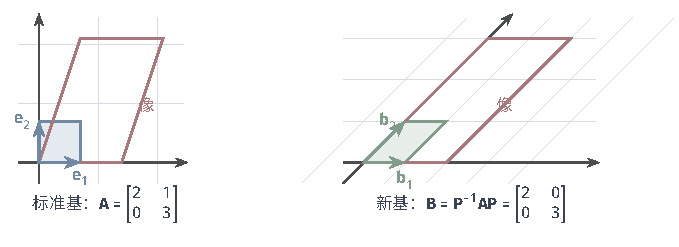
\includegraphics[width=112mm]{figures/01-mathematical-preliminaries-upper/03-linear-spaces/tikz/comprehension-additions/similarity-two-bases.pdf}
  \caption{同一个算子在两组基下的记录。左：标准基$\bm e_1,\bm e_2$围成的单位正方形（蓝）被$\bm A=\left[\begin{smallmatrix}2&1\\0&3\end{smallmatrix}\right]$送到红色平行四边形，形状被斜切。右：新基$\bm b_1=\bm e_1$、$\bm b_2=\bm e_1+\bm e_2$围成的平行四边形（绿）被同一个算子送到红色平行四边形，只沿$\bm b_1$伸长$2$倍、沿$\bm b_2$伸长$3$倍，因此新矩阵为$\operatorname{diag}(2,3)$。浅色斜线为新基网格。}
  \label{fig:ls-similarity-change-of-basis-flow}
\end{figure}

\paragraph{相似不变量}
\phantomsection
\label{sec:ls-similarity-properties}
同一个算子的性质不应随基改变；哪些量在相似下保持不变？相似首先是等价关系：$\bm A=\bm I^{-1}\bm A\bm I$给出自反性；由$\bm B=\bm P^{-1}\bm A\bm P$得$\bm A=\bm P\bm B\bm P^{-1}$，给出对称性；若再有$\bm C=\bm Q^{-1}\bm B\bm Q$，则$\bm C=(\bm P\bm Q)^{-1}\bm A(\bm P\bm Q)$，给出传递性。这三条分别对应不换基、换回原基和连续换两次基。

相似是相抵的特例，相抵不变量自然保持：$\operatorname{null}(\bm B)=\bm P^{-1}\operatorname{null}(\bm A)$，$\operatorname{range}(\bm B)=\bm P^{-1}\operatorname{range}(\bm A)$，因此
\begin{equation}
 \operatorname{rank}\bm B=\operatorname{rank}\bm A,
 \qquad
 \dim\operatorname{null}(\bm B)=\dim\operatorname{null}(\bm A).
 \label{eq:ls-similarity-invariants}
\end{equation}
算子还能反复作用，而先后作用与换基相容：若$\bm B_1=\bm P^{-1}\bm A_1\bm P$、$\bm B_2=\bm P^{-1}\bm A_2\bm P$，则
\begin{equation}
 \bm B_1\bm B_2
 =\bm P^{-1}\bm A_1\bm P\,\bm P^{-1}\bm A_2\bm P
 =\bm P^{-1}\bm A_1\bm A_2\bm P,
 \label{eq:ls-similarity-product}
\end{equation}
中间的$\bm P\bm P^{-1}$相消。归纳得$\bm B^k=\bm P^{-1}\bm A^k\bm P$：反复作用同一个算子，在新基下仍是同一过程的记录。同样，对任意实数$c$，$\bm B-c\bm I=\bm P^{-1}(\bm A-c\bm I)\bm P$，所以$\bm A-c\bm I$与$\bm B-c\bm I$也相似，由式~\eqref{eq:ls-similarity-invariants}，
\begin{equation}
 \operatorname{rank}(\bm B-c\bm I)=\operatorname{rank}(\bm A-c\bm I),\qquad c\in\mathbb R.
 \label{eq:ls-similarity-shifted-rank}
\end{equation}
这比总秩更细：它对每个$c$都给出一个不变量。

相似还保持两个可以直接计算的标量。由行列式的乘法性（第~\ref{sec:ls-determinant-properties}节）与$\det(\bm P^{-1})\det\bm P=\det\bm I=1$，
\[
 \det(\bm P^{-1}\bm A\bm P)=\det(\bm P^{-1})\,\det\bm A\,\det\bm P=\det\bm A;
\]
由迹的循环性（式~\eqref{eq:linear-algebra-trace-cyclic}），
\[
 \operatorname{tr}(\bm P^{-1}\bm A\bm P)=\operatorname{tr}\bigl((\bm A\bm P)\bm P^{-1}\bigr)=\operatorname{tr}\bm A.
\]
两式说明，行列式与迹只依赖算子本身，是判断两个矩阵能否记录同一算子时可以直接计算的两个标量不变量。例如示例~\ref{ex:ls-similarity-diagonal}中的$\bm A$与$\bm B=\operatorname{diag}(2,3)$行列式都是$6$，迹都是$5$。于是可以说“算子$T$的行列式”“算子$T$的迹”，用任意一组基下的矩阵计算即可。

引入特征值以后还将看到（第~\ref{sec:ls-eigen-similarity-invariance}节），特征值与特征多项式同样是相似不变量，而行列式与迹恰好是特征值之积与特征值之和。一般的换基不保持欧氏长度与夹角，这些度量量不在相似保持之列。

\paragraph{相似的判定}
\phantomsection
\label{sec:ls-similarity-conditions}
怎样判断两个给定的方阵是否相似？两端左乘$\bm P$，相似等价于存在\emph{可逆}的$\bm P$满足
\begin{equation}
 \bm A\bm P=\bm P\bm B.
 \label{eq:ls-similarity-equation}
\end{equation}
这是关于$\bm P$各元素的一组线性方程。只找到非零但不可逆的解还不够：那只是两个坐标子空间之间的对应，不是两组基之间的换基。

不变量给出否定的判据：只要某个相似不变量不同，两个矩阵就不相似。但秩、行列式、迹相同，都只是相似的必要条件，下面的例子说明它们合在一起也不够。
\begin{example}[反例：相抵而不相似的两个矩阵]
\label{ex:ls-equivalent-not-similar}
给定：$\bm I_2$与$\bm J=\left[\begin{smallmatrix}1&1\\0&1\end{smallmatrix}\right]$。

验证：二者都可逆，秩都为$2$，由相抵判据它们相抵；二者的行列式都是$1$，迹都是$2$。但取$c=1$，$\bm I_2-\bm I_2=\bm0$的秩为$0$，而$\bm J-\bm I_2=\left[\begin{smallmatrix}0&1\\0&0\end{smallmatrix}\right]$的秩为$1$，式~\eqref{eq:ls-similarity-shifted-rank}不成立。更直接地，若$\bm J=\bm P^{-1}\bm I_2\bm P$，则$\bm J=\bm P^{-1}\bm P=\bm I_2$，矛盾。

结论：$\bm I_2$与$\bm J$相抵，秩、行列式与迹也都相同，却不相似；单位矩阵只与自己相似。
\end{example}
这正是“两端换基相同”这一约束的代价：相抵时秩相同就足够，相似时连秩、行列式与迹一起相同都不够。比较$\bm A-c\bm I$在各个$c$处的秩是更细的必要条件；完整的相似分类需要Jordan标准形，本书不展开。

% 第5章第4节：对偶空间（线性泛函与对偶空间、对偶基、对偶映射与转置）。

\section{对偶空间}
\label{sec:ls-dual-spaces}

线性映射把对象送到另一个空间；还有一类最简单的作用，只把对象读成一个数。取多项式在某一点的值、取信号的第一个样本、计算一组特征的加权和，都是这样的读取；第~\ref{sec:ls-coordinates}节的坐标$x_j$也是，每个坐标都把对象读成一个数。第~\ref{chap:linear-operations}章在$\mathbb R^d$上用内积$\langle\bm w,\bm x\rangle$表示加权读取，读取规则借一个向量$\bm w$来写；一般空间上还没有内积，读取规则本身是什么对象，就需要单独回答。

本节讨论三个问题：全部线性读取组成怎样的空间；坐标作为读取，与基有怎样的关系；对象经过线性映射以后，输出端的读取怎样传回输入端。最后一个问题的答案是转置，它给第~\ref{chap:linear-operations}章中“行列互换”的操作一个不依赖坐标的含义。回答这三个问题只用到线性运算；本节最后借$\mathbb R^d$上的范数给读取规则规定大小，即对偶范数。

\subsection{线性泛函与对偶空间}
\label{sec:ls-dual-space}

\paragraph{线性泛函}
保持线性组合的标量读取称为\term{线性泛函}（linear functional）：映射$\varphi:V\to\mathbb R$满足
\[
 \varphi(a\bm x+b\bm y)=a\varphi(\bm x)+b\varphi(\bm y),\qquad \bm x,\bm y\in V,\ a,b\in\mathbb R.
\]
它就是陪域为$\mathbb R$的线性映射。在$P_k$上，取值$p\mapsto p(t_0)$与积分$p\mapsto\int_0^1p(t)\,\mathrm dt$都是线性泛函；在$\mathbb R^d$上，读取第$j$个坐标与加权和$\bm x\mapsto\bm a^\top\bm x$都是线性泛函。但并非每个把向量读成一个数的规则都是线性泛函。
\begin{example}[反例：两个非线性的读取]
\label{ex:ls-nonlinear-readouts}
给定：$\mathbb R^d$上的两个读取$\varphi_1(\bm x)=x_1+1$与$\varphi_2(\bm x)=\lVert\bm x\rVert_2$。

验证：线性泛函必把零向量读成$0$，而$\varphi_1(\bm0)=1$。线性泛函还满足$\varphi(-\bm x)=-\varphi(\bm x)$；但对任一$\bm x\neq\bm0$，$\varphi_2(-\bm x)=\lVert\bm x\rVert_2>0$，而$-\varphi_2(\bm x)<0$。

结论：$\varphi_1$与$\varphi_2$都不是线性泛函。
\end{example}

按线性映射的矩阵表示，选定$V$的基$\mathcal B=(\bm b_1,\ldots,\bm b_d)$、输出端取数$1$作基，线性泛函$\varphi$记录为$1\times d$矩阵
\[
 [\varphi]_{\mathcal B}=\bigl(\varphi(\bm b_1),\ \ldots,\ \varphi(\bm b_d)\bigr),
 \qquad
 \varphi(\bm v)=[\varphi]_{\mathcal B}[\bm v]_{\mathcal B}=\sum_{j=1}^dx_j\varphi(\bm b_j).
\]
对象的坐标是一列，读取规则的系数是一行，二者相乘得到读数。

非零泛函取到某个非零值，把相应的输入缩放即可取到任意实数，所以它的像是整个$\mathbb R$；由秩零度定理，它的核是$d-1$维子空间。读数等于$c$的点组成核的平移$\bm x_0+\ker\varphi$（其中$\varphi(\bm x_0)=c$），在平面上就是一族平行直线。

\paragraph{对偶空间}
同一个对象可以接受多种读取，两种读取也可以组合：规定
\[
 (\alpha\varphi+\beta\psi)(\bm x)=\alpha\varphi(\bm x)+\beta\psi(\bm x),
\]
右端对$\bm x$仍保持线性组合，所以线性泛函的线性组合仍是线性泛函。全部线性泛函在这两种运算下构成线性空间，称为$V$的\term{对偶空间}（dual space），记为$V^*$。输入向量是被读取的对象，泛函是读取规则，二者属于不同的空间；即使在$\mathbb R^d$中一行系数与一列坐标的数字相同，也不能直接相加。

\paragraph{对偶基}
$V^*$有多大？坐标给出了一组现成的读取。对$V$的有序基$\mathcal B=(\bm b_1,\ldots,\bm b_d)$，第$j$个坐标$\bm v\mapsto x_j$是线性泛函（坐标映射保持线性组合），记为$\varphi_j$。由$\bm b_i$的坐标是$\bm e_i$，
\begin{equation}
 \varphi_j(\bm b_i)=\delta_{j,i}
 =\begin{cases}1,&i=j,\\0,&i\neq j.\end{cases}
 \label{eq:ls-dual-basis-def}
\end{equation}
反过来，线性泛函由它在基向量上的值决定，所以式~\eqref{eq:ls-dual-basis-def}也可以当作$\varphi_j$的定义。

这$d$个读取构成$V^*$的一组基。任意$\varphi\in V^*$都能写成
\[
 \varphi=\sum_{j=1}^d\varphi(\bm b_j)\,\varphi_j,
\]
因为两边在每个$\bm b_i$上取值都是$\varphi(\bm b_i)$，而线性泛函由基向量上的值决定；若$\sum_ja_j\varphi_j=0$，在$\bm b_i$上取值得$a_i=0$，所以它们线性无关。这组$\varphi_1,\ldots,\varphi_d$称为$\mathcal B$的\term{对偶基}（dual basis），于是$\dim V^*=\dim V$。读取$\varphi$在对偶基下的坐标正是它在各基向量上的读数$\varphi(\bm b_j)$，即上面那一行系数。

对偶基的每个成员依赖整组基，而不只依赖对应的那个基向量。
\begin{example}[改变第二个基向量会改变第一个坐标读取]
\label{ex:ls-dual-basis-depends-on-basis}
给定：$\mathbb R^2$的标准基$(\bm e_1,\bm e_2)$与基$(\bm e_1,\bm e_1+\bm e_2)$。

计算：标准基的对偶基是两个坐标读取$\varphi_1(x,y)=x$、$\varphi_2(x,y)=y$。在第二组基下，
\[
 (x,y)^\top=(x-y)\bm e_1+y(\bm e_1+\bm e_2),
\]
所以第一个坐标读取变成$x-y$，第二个坐标读取仍是$y$。

结论：两组基的第一个向量都是$\bm e_1$，相应的第一个对偶读取却从$x$变成了$x-y$。
\end{example}
对一般的基，对偶基要由方程组$\varphi_j(\bm b_i)=\delta_{j,i}$解出。
\begin{example}[斜基的对偶基]
\label{ex:ls-dual-basis-oblique}
给定：$\mathbb R^2$的基$\bm b_1=(2,1)^\top$、$\bm b_2=(-1,1)^\top$，以及读取横坐标的泛函$\ell(x,y)=x$。

计算：设$\varphi_1(x,y)=\alpha x+\beta y$。条件$\varphi_1(\bm b_1)=2\alpha+\beta=1$与$\varphi_1(\bm b_2)=-\alpha+\beta=0$给出$\alpha=\beta=1/3$；同样由$\varphi_2(\bm b_1)=0$、$\varphi_2(\bm b_2)=1$解出$\varphi_2$，得
\[
 \varphi_1(x,y)=\frac{x+y}3,\qquad \varphi_2(x,y)=\frac{-x+2y}3 .
\]
$\ell$在基向量上的读数为$\ell(\bm b_1)=2$、$\ell(\bm b_2)=-1$，所以$\ell=2\varphi_1-\varphi_2$。代入验证：$\tfrac23(x+y)-\tfrac13(-x+2y)=x$。

结论：$\ell$在对偶基下的坐标是$(2,-1)$，正是它在两个基向量上的读数。
\end{example}
图~\ref{fig:ls-dual-basis-readout}画出这些读取：每个对偶读取只在一个基向量上读到$1$，在另一个基向量上读到$0$。
\begin{figure}[htbp]
  \centering
  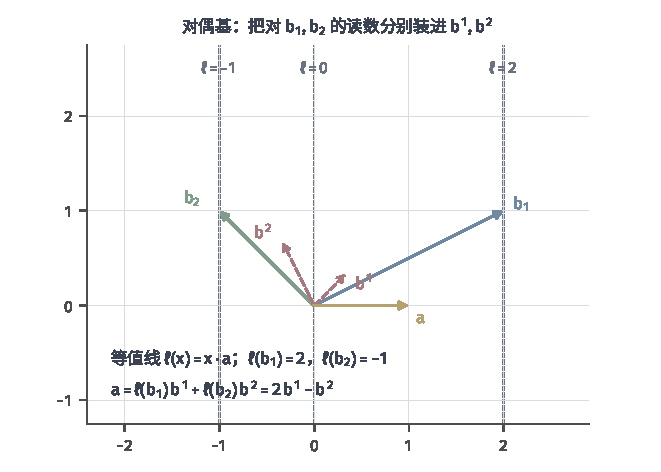
\includegraphics[width=112mm]{figures/01-mathematical-preliminaries-upper/03-linear-spaces/matplotlib/ls-dual-basis-readout/ls-dual-basis-readout.pdf}
  \caption{对偶读取的几何示意。蓝箭头$\bm b_1=(2,1)$、绿箭头$\bm b_2=(-1,1)$为基向量；红色虚线箭头$\bm b^1=(1/3,1/3)$、$\bm b^2=(-1/3,2/3)$分别是对偶基$\varphi_1,\varphi_2$的系数向量，即$\varphi_i(\bm x)=\bm b^i\cdot\bm x$，满足$\varphi_i(\bm b_j)=\delta_{i,j}$。把读取规则画成平面箭头借用了标准内积，这一对应在第~\ref{sec:ls-riesz-representation}节说明。黄色箭头$\bm a=(1,0)$给出读取$\ell(\bm x)=\bm a\cdot\bm x$，灰色虚线为等值线$\ell=c$（$c=-1,0,2$）；$\ell(\bm b_1)=2$、$\ell(\bm b_2)=-1$，且$\bm a=2\bm b^1-\bm b^2$。}
  \label{fig:ls-dual-basis-readout}
\end{figure}

换基时，读取系数与坐标的变化方向相反。设新基$\mathcal B'$由换基矩阵$\bm P=\bm S_{\mathcal B\leftarrow\mathcal B'}$给出，即$\bm b'_j=\sum_i\bm P_{i,j}\bm b_i$。坐标按$[\bm v]_{\mathcal B'}=\bm P^{-1}[\bm v]_{\mathcal B}$变化；读取系数则按$\varphi(\bm b'_j)=\sum_i\varphi(\bm b_i)\bm P_{i,j}$变化，即$[\varphi]_{\mathcal B'}=[\varphi]_{\mathcal B}\bm P$。二者相乘时$\bm P$与$\bm P^{-1}$相消，读数$\varphi(\bm v)$不随基改变，这正是读数应有的性质。

\subsection{对偶映射}
\label{sec:ls-dual-map}

已知线性映射$T:V\to W$和输出端的一个读取$f\in W^*$，输入$\bm x$经过$T$以后被读成$f(T\bm x)$。先作用、再读取，合起来是输入端的一个读取。由这一复合定义\term{对偶映射}（dual map）$T':W^*\to V^*$：
\begin{equation}
 T'f=f\circ T,\qquad (T'f)(\bm x)=f(T\bm x).
 \label{eq:ls-dual-map-def}
\end{equation}
$T'$保持线性组合：$(T'(\alpha f+\beta g))(\bm x)=\alpha f(T\bm x)+\beta g(T\bm x)$。对象从$V$走到$W$，读取则从$W^*$传回$V^*$，方向相反；这只是把读取规则搬回输入端，并不是对$T$求逆。复合时次序也随之反转：对$S:W\to U$，$(S\circ T)'f=f\circ S\circ T=T'(S'f)$，即$(S\circ T)'=T'\circ S'$。

\paragraph{对偶映射的矩阵是转置}
设输入基$\mathcal B=(\bm b_1,\ldots,\bm b_d)$、输出基$\mathcal C=(\bm c_1,\ldots,\bm c_m)$下$T$的矩阵为$\bm A$，即$T\bm b_j=\sum_ka_{k,j}\bm c_k$；两组基的对偶基分别记为$\varphi_1,\ldots,\varphi_d$与$\psi_1,\ldots,\psi_m$。取输出读取$f=\sum_iy_i\psi_i$，它传回输入端以后，在输入基向量上的读数是
\[
 (T'f)(\bm b_j)=f(T\bm b_j)
 =\sum_iy_i\,\psi_i\Bigl(\sum_ka_{k,j}\bm c_k\Bigr)
 =\sum_ia_{i,j}y_i=(\bm A^\top\bm y)_j .
\]
上一小节说明，读取在对偶基下的坐标就是它在各基向量上的读数，所以$T'f$的坐标为$\bm A^\top\bm y$：在对偶基下，对偶映射的矩阵是$\bm A^\top$。转置的乘积规则$(\bm B\bm A)^\top=\bm A^\top\bm B^\top$正是$(S\circ T)'=T'\circ S'$的坐标记录。下面用一个具体映射核对这一结论。
\begin{example}[把输出的第一个分量读取传回输入端]
\label{ex:ls-dual-map-first-component}
给定：$T(x_1,x_2)=(2x_1+x_2,\ 3x_2)$，它在标准基下的矩阵为$\bm A=\left[\begin{smallmatrix}2&1\\0&3\end{smallmatrix}\right]$；输出端读取第一个分量，即$f=\psi_1$，系数$\bm y=(1,0)^\top$。

计算：先作用再读取，$(T'f)(\bm x)=f(T\bm x)=2x_1+x_2$，系数为$(2,1)^\top$。按矩阵计算，$\bm A^\top(1,0)^\top=(2,1)^\top$。

结论：两种算法一致，传回的读取系数正是$\bm A$的第一行。
\end{example}
一般地，读取输出第$i$个分量并传回输入端，得到的读取系数就是$\bm A$的第$i$行，所以$T'$的像在坐标下就是行空间。

\paragraph{再证行秩等于列秩}
对偶映射给出定理~\ref{thm:ls-row-rank-column-rank}的一个不依赖消元的证明。先看$T'$的核。$T'f=0$意味着$f(T\bm x)=0$对一切$\bm x$成立，即$f$在$\operatorname{im}T$上恒为零：$\ker T'$由看不见任何可达输出的读取组成，在坐标下就是$\bm A^\top\bm y=\bm0$，即左零空间。

再算它的维数。设$r=\operatorname{rank}T$，取$\operatorname{im}T$的基$\bm c_1,\ldots,\bm c_r$并扩充为$W$的基$\bm c_1,\ldots,\bm c_m$，对偶基为$\psi_1,\ldots,\psi_m$。读取$f=\sum_iy_i\psi_i$在$\operatorname{im}T$上恒为零，当且仅当它在$\bm c_1,\ldots,\bm c_r$上都读到零，即$y_1=\cdots=y_r=0$，所以$\ker T'=\operatorname{span}\{\psi_{r+1},\ldots,\psi_m\}$，维数为$m-r$。对$T':W^*\to V^*$用秩零度定理，$\operatorname{rank}T'=\dim W^*-\dim\ker T'=m-(m-r)=r$。$T'$的矩阵是$\bm A^\top$，于是$\operatorname{rank}\bm A^\top=\operatorname{rank}\bm A$。

至此，读取规则有了自己的空间、坐标和传递规律。还有两个问题没有回答。一个读取有多“大”，即输入有界时读数最多有多大？这要先度量输入的大小：在$\mathbb R^d$上可以借第~\ref{chap:linear-operations}章的范数回答，这就是下一小节的对偶范数；一般空间则要等下一节定义范数以后回答（第~\ref{sec:ls-finite-dimensional-sequences}节）。一个读取能否写成与某个固定向量的配对？这要用到内积，在第~\ref{sec:ls-riesz-representation}节回答。

\subsection{对偶范数}
\label{sec:ls-dual-norms}

前两小节只用到线性运算。若$V=\mathbb R^d$上已经取定第~\ref{chap:linear-operations}章的某种范数，还可以问一个读取规则有多“大”。这正是误差分析中的常见问题：误差$\bm r$只知道落在某个范数球内时，一次加权读取$\bm z^\top\bm r$最多变化多少？下面的量就是这个最大值。
\begin{definition}[对偶范数]
\label{def:linear-algebra-dual-norm}
给定$\mathbb R^d$上的范数，相对于标准坐标配对的\term{对偶范数}（dual norm）为
\begin{equation}
 \lVert\bm z\rVert_*=\sup_{\lVert\bm r\rVert\leq1}|\bm z^\top\bm r|.
 \label{eq:linear-algebra-dual-norm-definition}
\end{equation}
\end{definition}
对任意范数，这个上确界有限并可以取到（第~\ref{sec:ls-error-scale-comparison}节）；对$\ell_p$范数，下面还将直接构造取到它的$\bm r$。它满足范数的四条要求，因而是对偶空间上的范数。非负性显然。$\bm z\neq\bm0$时，取$\bm z$的某个非零坐标$z_j$，$\bm r=\bm e_j/\lVert\bm e_j\rVert$给出$|\bm z^\top\bm r|=|z_j|/\lVert\bm e_j\rVert>0$。对每个$\bm r$都有$|(\bm z+\bm w)^\top\bm r|\leq|\bm z^\top\bm r|+|\bm w^\top\bm r|$，取上确界即得三角不等式；齐次性由$|(c\bm z)^\top\bm r|=|c|\,|\bm z^\top\bm r|$得到。图~\ref{fig:ls-dual-norm-unit-ball}把这个最大值画成支撑线最后接触单位球的位置。

\begin{figure}[!htb]
  \centering
  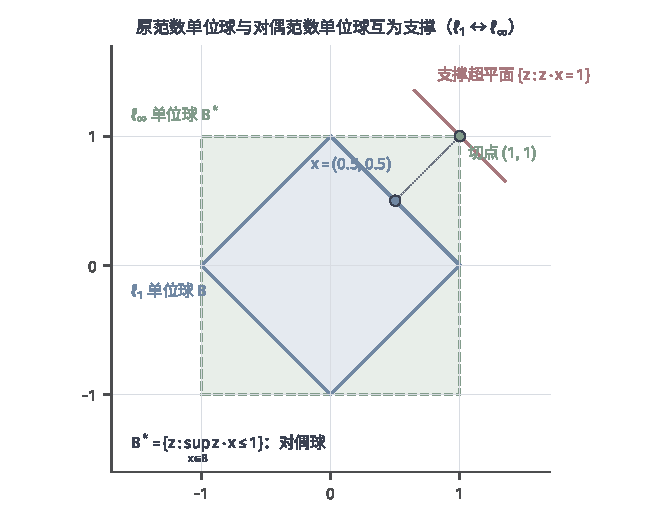
\includegraphics[width=112mm]{figures/01-mathematical-preliminaries-upper/03-linear-spaces/matplotlib/ls-dual-norm-unit-ball/ls-dual-norm-unit-ball.pdf}
  \caption{对偶范数的几何：在原范数单位球$\lVert\bm r\rVert\leq1$上求线性读取$\bm z^\top\bm r$的最大值。左：原单位球（灰色）与读取方向$\bm z$；右：支撑直线最后接触单位球处给出$\lVert\bm z\rVert_*=\max_{\lVert\bm r\rVert\leq1}|\bm z^\top\bm r|$。对偶单位球（虚线）与原单位球互为极体，为解析教学例。}
  \label{fig:ls-dual-norm-unit-ball}
\end{figure}

对$\ell_p$范数，
\begin{equation}
 (\lVert\cdot\rVert_p)_*=\lVert\cdot\rVert_q,\qquad \frac1p+\frac1q=1,
 \label{eq:linear-algebra-lp-duality}
\end{equation}
并且由齐次性，对$\rho\geq0$有
\begin{equation}
 \max_{\lVert\bm r\rVert_p\leq\rho}|\bm z^\top\bm r|
 =\rho\lVert\bm z\rVert_q.
 \label{eq:linear-algebra-linear-perturbation-duality}
\end{equation}
第~\ref{chap:linear-operations}章的Hölder不等式（定理~\ref{thm:linear-algebra-holder}）给出$\ell_p$单位球上的上界$\lVert\bm z\rVert_q$。这个上界可以达到：$1<p<\infty$时取$r_j=|z_j|^{q-1}\operatorname{sgn}(z_j)/\lVert\bm z\rVert_q^{q-1}$；$p=1$时把单位预算全部放在$|z_j|$最大的坐标上；$p=\infty$时逐坐标取$r_j=\operatorname{sgn}(z_j)$。下面固定一个读取，比较三种误差预算。
\begin{example}[同一读取在三种误差预算下的最大变化]
\label{ex:ls-dual-norm-three-budgets}
给定：读取方向$\bm z=(2,-1)^\top$，即读取$\bm z^\top\bm r=2r_1-r_2$。

计算：在$\ell_1$单位球上，把单位预算全部放在$|z_j|$最大的第一个坐标，$\bm r=(1,0)^\top$给出最大值$\lVert\bm z\rVert_\infty=2$。在$\ell_2$单位球上，取$\bm r=\bm z/\lVert\bm z\rVert_2=(2,-1)^\top/\sqrt5$，最大值为$\lVert\bm z\rVert_2=\sqrt5$。在$\ell_\infty$单位球上，逐坐标取$r_j=\operatorname{sgn}(z_j)$，$\bm r=(1,-1)^\top$给出最大值$\lVert\bm z\rVert_1=3$。若误差预算为$|r_j|\leq0.01$，在式~\eqref{eq:linear-algebra-linear-perturbation-duality}中取$p=\infty$、$\rho=0.01$，最大变化为$0.01\cdot(2+1)=0.03$，由$\bm r=(0.01,-0.01)^\top$达到。

结论：同一次读取在$\ell_1$、$\ell_2$、$\ell_\infty$单位球上的最大值依次为$2$、$\sqrt5$、$3$；改变误差预算的形状，最坏方向和最大变化都随之改变。
\end{example}
图~\ref{fig:linear-algebra-dual-unit-balls}画出这三种情形下的最坏方向。
\begin{figure*}[htbp]
  \centering
  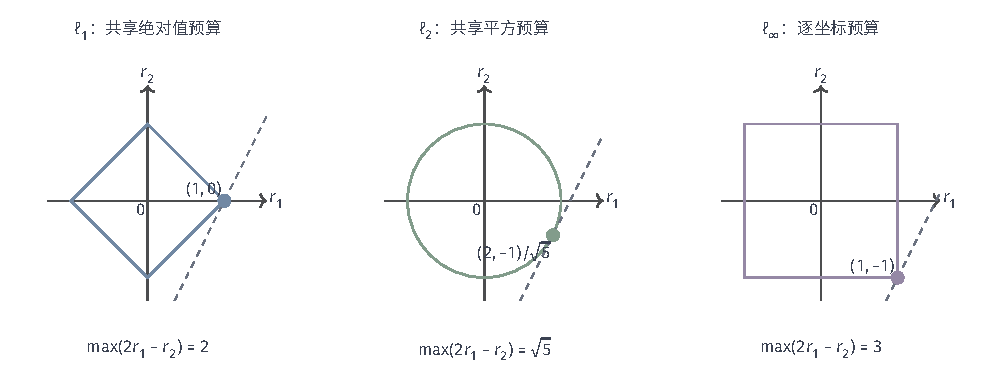
\includegraphics[width=168.998mm]{figures/01-mathematical-preliminaries-upper/03-linear-spaces/tikz/linear-algebra-dual-unit-balls/figure.pdf}
  \caption{同一线性读取$2r_1-r_2$在$\ell_1$、$\ell_2$、$\ell_\infty$单位球上的最大值依次为$2$、$\sqrt5$、$3$。虚线为最后接触可行集的支撑直线，点为最大化方向。三图坐标尺度相同，均为解析教学例；改变允许误差的形状会改变误差常数。}
  \label{fig:linear-algebra-dual-unit-balls}
\end{figure*}

误差预算按$\ell_\infty$给出时，读取方向要按$\ell_1$计量；预算按$\ell_2$给出时，读取方向仍按$\ell_2$计量。所以讨论“输入误差最多引起多大输出误差”时，必须先说清误差用哪种范数度量。

% 第5章第5节：赋范空间（范数与收敛、有限维赋范空间、完备性与Banach空间），只讨论有限维情形。

\section{赋范空间}
\label{sec:ls-normed-spaces}

前四节只用到加法与数乘，回答的都是“能否表示、是否唯一、有几个方向”这类是非与计数问题，还没有“大小”。可是用一个多项式近似一个函数时，要问误差有多大；一列近似越来越好时，要问它们是否趋于某个对象，那个对象是否仍在原来的空间里；上一节的读取也要问，输入不大时读数最多有多大。第~\ref{chap:linear-operations}章用范数度量$\mathbb R^d$中数组的大小（第~\ref{sec:ls-norms-distances}节），本节把它推广到一般线性空间。

本节回答三个问题：范数怎样给出收敛；有限维空间中，选哪个范数会不会影响收敛与否；收敛序列的极限什么时候一定留在空间中。前两个问题在有限维中有干净的答案：一切范数等价，收敛就是逐坐标收敛。第三个问题引出完备性与Banach空间，它在有限维中自动成立。本节只讨论有限维空间；无限维空间中这三个问题的答案都会改变，留到后面的章节。

\subsection{范数与赋范空间}
\label{sec:ls-normed-space-definition}

\paragraph{范数的定义}
第~\ref{chap:linear-operations}章的$\ell_1$、$\ell_2$、$\ell_\infty$范数各有侧重，却满足同样的几条要求：大小非负，只有零向量大小为零，整体放大$c$倍时大小放大$|c|$倍，两段误差相加时总大小不超过各自大小之和。这些要求只用到加法与数乘，因此可以直接作为一般线性空间上“大小”的要求。
\begin{definition}[赋范空间]
\label{def:ls-normed-space}
设$V$是实线性空间。映射$\lVert\cdot\rVert:V\to[0,\infty)$若对任意$\bm x,\bm y\in V$与$c\in\mathbb R$满足
\begin{enumerate}
 \item 正定性：$\lVert\bm x\rVert=0$当且仅当$\bm x=\bm0$；
 \item 齐次性：$\lVert c\bm x\rVert=|c|\,\lVert\bm x\rVert$；
 \item 三角不等式：$\lVert\bm x+\bm y\rVert\leq\lVert\bm x\rVert+\lVert\bm y\rVert$，
\end{enumerate}
就称为$V$上的范数；配备范数的线性空间$(V,\lVert\cdot\rVert)$称为\term{赋范空间}（normed space）。
\end{definition}
范数诱导距离$d(\bm x,\bm y)=\lVert\bm x-\bm y\rVert$：它非负，只在$\bm x=\bm y$时为零，对称，并满足$d(\bm x,\bm z)\leq d(\bm x,\bm y)+d(\bm y,\bm z)$。这些性质也是第~\ref{chap:metric-spaces}章度量空间的公理，所以赋范空间是一类特殊的度量空间。它的距离还与线性运算相容：平移不改变距离，缩放把距离按比例缩放。

把三角不等式用于$\bm x=(\bm x-\bm y)+\bm y$，得$\lVert\bm x\rVert-\lVert\bm y\rVert\leq\lVert\bm x-\bm y\rVert$；交换$\bm x,\bm y$的角色，又得$\lVert\bm y\rVert-\lVert\bm x\rVert\leq\lVert\bm x-\bm y\rVert$。两式合起来就是反向三角不等式
\begin{equation}
 \bigl|\lVert\bm x\rVert-\lVert\bm y\rVert\bigr|\leq\lVert\bm x-\bm y\rVert,
 \label{eq:ls-reverse-triangle}
\end{equation}
它说明两个向量相距很近时，长度也相差很少。

\paragraph{例子}
$\mathbb R^d$上的$p$范数、同形矩阵上的Frobenius范数与诱导矩阵范数都是范数，第~\ref{chap:linear-operations}章已经验证。一般空间上，最直接的办法是借坐标：若$\lVert\cdot\rVert_\star$是$\mathbb R^d$上的范数，$\mathcal B$是$V$的基，则$\lVert\bm v\rVert=\lVert[\bm v]_{\mathcal B}\rVert_\star$是$V$上的范数，因为坐标映射是保持线性组合的双射。也可以不经过坐标，直接用对象本身的性质规定范数。下面在$P_k$上各举一例。
\begin{example}[多项式空间上的两个范数]
\label{ex:ls-polynomial-norms}
给定：$P_k$上的两个规则：对$p=a_0+a_1t+\cdots+a_kt^k$，
\[
 p\mapsto\max_{0\leq j\leq k}|a_j|,
 \qquad
 p\mapsto\lVert p\rVert_\infty=\max_{t\in[0,1]}|p(t)| .
\]

验证：第一个规则是坐标$(a_0,\ldots,a_k)$在基$(1,t,\ldots,t^k)$下的$\ell_\infty$范数，按上面的借坐标方法是范数。对第二个规则，齐次性逐点成立；三角不等式来自$|p(t)+q(t)|\leq|p(t)|+|q(t)|\leq\lVert p\rVert_\infty+\lVert q\rVert_\infty$对每个$t$成立，再对$t$取最大值；正定性来自次数不超过$k$的非零多项式至多有$k$个根，不能在整个区间$[0,1]$上为零。

结论：二者都是$P_k$上的范数，前者经过坐标，后者直接用函数值。
\end{example}

\paragraph{收敛}
有了距离，就可以说一列向量趋于某个向量。在赋范空间中，若实数列$\lVert\bm x_n-\bm x\rVert\to0$，就说$\bm x_n$按该范数\emph{收敛}到$\bm x$，记为$\bm x_n\to\bm x$。极限若存在则唯一：若$\bm x_n\to\bm x$且$\bm x_n\to\bm y$，则$\lVert\bm x-\bm y\rVert\leq\lVert\bm x-\bm x_n\rVert+\lVert\bm x_n-\bm y\rVert\to0$。由式~\eqref{eq:ls-reverse-triangle}，$\bm x_n\to\bm x$时还有$\lVert\bm x_n\rVert\to\lVert\bm x\rVert$。

收敛的定义依赖所选的范数：不同范数给出的误差读数不同，同一个序列会不会在一种范数下收敛、在另一种范数下不收敛？下一小节说明，有限维空间中不会出现这种情形。

\subsection{有限维赋范空间}
\label{sec:ls-finite-dimensional-sequences}
\label{sec:linear-algebra-sequence-convergence}
\label{sec:ls-error-scale-comparison}

讨论向量序列的收敛，先要选一个范数测量误差。$\ell_1$、$\ell_2$、$\ell_\infty$或某个加权范数给出的误差读数各不相同。本小节证明，在有限维空间中任意两个范数最多相差常数倍，因而收敛与否、极限是什么都与范数无关；证明要把第~\ref{chap:function-limits}章有界实数列的Bolzano--Weierstrass定理逐坐标用于向量序列。由此还得到线性映射的连续性、子空间的闭性与最近点的存在。

\paragraph{闭集与有界集}
在赋范空间中，若存在$R$使$\lVert\bm x\rVert\leq R$对集合$K$中的一切$\bm x$成立，就称$K$\emph{有界}；若$K$中任何收敛序列的极限仍属于$K$，就称$K$\emph{闭}。在实轴上，这一闭性与第~\ref{chap:function-limits}章用补集定义的闭集一致（引理~\ref{lem:analysis-closed-sequence-criterion}）；一般度量空间中的开闭集在第~\ref{chap:metric-spaces}章讨论。

闭球$\{\bm x:\lVert\bm x\rVert\leq r\}$是闭集：若$\lVert\bm x_n\rVert\leq r$且$\bm x_n\to\bm x$，则$\lVert\bm x\rVert=\lim_n\lVert\bm x_n\rVert\leq r$。同理，单位球面$\{\bm x:\lVert\bm x\rVert=1\}$是闭有界集。若$K\subseteq V$上的函数$f$满足：只要$K$中的$\bm x_n\to\bm x\in K$，就有$f(\bm x_n)\to f(\bm x)$，就称$f$在$K$上连续。由式~\eqref{eq:ls-reverse-triangle}，范数本身是连续函数。

\paragraph{范数等价}
现在比较同一个有限维空间上的两个范数。
\begin{theorem}[有限维范数等价]
\label{thm:ls-norm-equivalence}
有限维实线性空间上任意两个范数$p,q$都等价：存在常数$c,C>0$，使$c\,q(\bm x)\leq p(\bm x)\leq C\,q(\bm x)$对所有$\bm x$成立。
\end{theorem}
\begin{proof}
思路是把每个范数都与一个固定的参照范数比较。固定基$(\bm b_1,\ldots,\bm b_d)$，把$\bm x=\sum_jx_j\bm b_j$等同于坐标向量$(x_1,\ldots,x_d)$，取坐标最大范数$\lVert\bm x\rVert_c=\max_j|x_j|$作参照。按它收敛就是逐坐标收敛：$\lVert\bm x_n-\bm x\rVert_c\to0$当且仅当每个坐标$x_{n,j}\to x_j$，因为最大值趋于零当且仅当有限个坐标差都趋于零。

上界。对任意范数$p$，由三角不等式与齐次性，
\[
 p(\bm x)=p\Bigl(\sum_jx_j\bm b_j\Bigr)\leq\sum_j|x_j|\,p(\bm b_j)\leq C_p\lVert\bm x\rVert_c,
 \qquad C_p=\sum_jp(\bm b_j).
\]

下界。由反向三角不等式，$|p(\bm x)-p(\bm y)|\leq p(\bm x-\bm y)\leq C_p\lVert\bm x-\bm y\rVert_c$，所以只要$\lVert\bm x_n-\bm x\rVert_c\to0$，就有$p(\bm x_n)\to p(\bm x)$。考虑坐标单位球面$S=\{\bm x:\lVert\bm x\rVert_c=1\}$，记$m_p=\inf_{\bm x\in S}p(\bm x)\geq0$，对每个$n$取$\bm x_n\in S$使$p(\bm x_n)<m_p+1/n$。这列向量的每个坐标都满足$|x_{n,j}|\leq1$，是有界实数列。由Bolzano--Weierstrass定理~\ref{thm:analysis-bounded-subsequence}，先在第一坐标上抽出收敛子列，再在这个子列中按第二坐标继续抽取，如此重复$d$次，最后得到的子列$\bm x_{n_k}$在每个坐标上都收敛。记各坐标的极限组成的向量为$\bm x^\star$，则$\lVert\bm x_{n_k}-\bm x^\star\rVert_c\to0$；由$\lVert\cdot\rVert_c$的反向三角不等式，$\lVert\bm x^\star\rVert_c=\lim_k\lVert\bm x_{n_k}\rVert_c=1$，即$\bm x^\star\in S$。再由上面$p$的连续性，\phantomsection\label{thm:ls-extreme-value}$p(\bm x^\star)=\lim_kp(\bm x_{n_k})=m_p$，即$p$在$S$上取到最小值$m_p$。由$\lVert\bm x^\star\rVert_c=1$知$\bm x^\star\neq\bm0$，范数的正定性保证$m_p=p(\bm x^\star)>0$。对任意$\bm x\neq\bm0$，$\bm x/\lVert\bm x\rVert_c$在$S$上，由齐次性得$p(\bm x)\geq m_p\lVert\bm x\rVert_c$。合起来，
\begin{equation}
 m_p\lVert\bm x\rVert_c\leq p(\bm x)\leq C_p\lVert\bm x\rVert_c.
 \label{eq:linear-algebra-finite-norm-equivalence}
\end{equation}

最后比较$p$与$q$：$p\leq C_p\lVert\cdot\rVert_c\leq(C_p/m_q)\,q$，交换$p,q$的角色得反向不等式。
\end{proof}
定理中的常数依赖维数与所选范数。看$\ell_1$与$\ell_\infty$这一对。
\begin{example}[$\ell_1$与$\ell_\infty$范数的等价常数]
\label{ex:ls-l1-linf-constants}
给定：$\mathbb R^d$上的$\lVert\bm x\rVert_1=\sum_j|x_j|$与$\lVert\bm x\rVert_\infty=\max_j|x_j|$。

验证：$d$个非负数$|x_1|,\ldots,|x_d|$之和不小于其中最大的一个，又不超过最大者的$d$倍，所以
\[
 \lVert\bm x\rVert_\infty\leq\lVert\bm x\rVert_1\leq d\lVert\bm x\rVert_\infty .
\]
取$\bm x=\bm e_1$，两个范数都为$1$，左边取等号；取$\bm x=(1,\ldots,1)^\top$，$\lVert\bm x\rVert_1=d$、$\lVert\bm x\rVert_\infty=1$，右边取等号。

结论：常数$1$与$d$都不能改进；维数越大，同一误差在两种范数下的读数可以相差越多。
\end{example}
证明中真正用到有限维的是下界：坐标只有有限个，逐坐标抽取$d$次才得到在每个坐标上都收敛的子列，从而在单位球面上取到正的最小值。

\paragraph{收敛与连续性}
由范数等价，$\lVert\bm x_n-\bm x\rVert\to0$当且仅当$\lVert\bm x_n-\bm x\rVert_c\to0$，即每个坐标$x_{n,j}\to x_j$。因此在有限维空间中，序列是否收敛、收敛到哪里，都与所选范数和基无关，后文可以按论证方便选用范数。矩阵序列看作$\mathbb R^{m\times n}$中的向量，结论相同：$\bm A_k\to\bm A$在任意矩阵范数下都等价于逐元素收敛。

闭集与有界集同样与范数无关：两个范数只差常数倍，一个范数下有界的集合在另一个范数下也有界，收敛序列也完全相同。于是下界证明中的逐坐标抽取对任何范数都适用：有界序列的坐标有界，可以抽出收敛子列；若序列取自闭集，极限仍在集合内。

由此得到闭有界集上连续函数的最值。设$f$是非空闭有界集$K$上的连续函数，$m=\inf_{K}f$。取$K$中的序列$\bm x_n$，使$f(\bm x_n)\to m$（若$m=-\infty$，则使$f(\bm x_n)\to-\infty$），从中抽出收敛子列$\bm x_{n_k}\to\bm x^\star$；由闭性，$\bm x^\star\in K$。由连续性，$f(\bm x_{n_k})\to f(\bm x^\star)$。若$m=-\infty$，这个有限极限与$f(\bm x_{n_k})\to-\infty$矛盾，所以$m$有限；于是$f(\bm x^\star)=\lim_kf(\bm x_{n_k})=m$，即下确界可以取到。上确界同理。下面几处“可以达到”都由这一论证得到。

线性映射也自动连续。设$T:V\to W$是有限维赋范空间之间的线性映射，固定$V$的基并沿用证明中的记号。由三角不等式与齐次性，
\[
 \lVert T\bm x\rVert_W\leq\sum_j|x_j|\,\lVert T\bm b_j\rVert_W\leq C\lVert\bm x\rVert_c\leq\frac C{m_V}\lVert\bm x\rVert_V,
 \qquad C=\sum_j\lVert T\bm b_j\rVert_W,
\]
其中$m_V>0$是式~\eqref{eq:linear-algebra-finite-norm-equivalence}中$\lVert\cdot\rVert_V$的下界常数。于是$\lVert T\bm x_n-T\bm x\rVert_W\leq(C/m_V)\lVert\bm x_n-\bm x\rVert_V$，$T$连续。

上式还说明比值$\lVert T\bm x\rVert_W/\lVert\bm x\rVert_V$有界。由上面的最值论证，连续函数$\bm x\mapsto\lVert T\bm x\rVert_W$在闭且有界的单位球面上取到最大值，所以第~\ref{chap:linear-operations}章诱导矩阵范数定义中的上确界有限且可以达到。取$W=\mathbb R$，就回答了上一节留下的问题：线性泛函$\varphi$的大小可以定义为
\[
 \lVert\varphi\rVert_*=\sup_{\lVert\bm x\rVert\leq1}|\varphi(\bm x)|,
\]
它有限并且取到，是对偶空间$V^*$上的范数；在$\mathbb R^d$上，$\varphi(\bm x)=\bm z^\top\bm x$时它正是第~\ref{sec:ls-dual-norms}节的对偶范数$\lVert\bm z\rVert_*$。

\paragraph{子空间的闭性与商范数}
\phantomsection
\label{sec:ls-quotient-norms}
点到子空间的距离为零，是否意味着点就在子空间里？这取决于子空间是否闭。
\begin{theorem}[有限维子空间闭性]
\label{thm:ls-subspace-closed}
有限维赋范空间的每个线性子空间$U$都是闭集：若$\bm x_n\in U$且$\bm x_n\to\bm x$，则$\bm x\in U$。
\end{theorem}
\begin{proof}
把$U$的基扩充为整个空间的基，则$\bm x_n$在补充方向上的坐标恒为零。收敛等价于逐坐标收敛，所以$\bm x$在补充方向上的坐标是零序列的极限，仍为零，于是$\bm x\in U$。
\end{proof}
记点到子空间的距离为$d(\bm x,U)=\inf_{\bm u\in U}\lVert\bm x-\bm u\rVert$。若$d(\bm x,U)=0$，可在$U$中取$\bm u_n$使$\lVert\bm x-\bm u_n\rVert\to0$，由闭性$\bm x\in U$；反之显然。所以$d(\bm x,U)=0$当且仅当$\bm x\in U$。

这一结论保证了商空间上也能度量大小。第~\ref{sec:ls-quotient-spaces}节的商空间$V/U$把相差$U$中向量的点看成同一个类$\bm x+U$，那里只建立了线性结构。同一类中各点到$U$的距离相同：若$\bm x'=\bm x+\bm u_0$，$\bm u_0\in U$，则$\bm u$遍历$U$时$\bm u-\bm u_0$也遍历$U$，所以$d(\bm x',U)=d(\bm x,U)$。因此可以把这个距离当作类的大小，称为商范数
\[
 \lVert\bm x+U\rVert_{V/U}=d(\bm x,U)=\inf_{\bm u\in U}\lVert\bm x-\bm u\rVert .
\]
它满足范数的三条要求。三角不等式：对任意$\bm u,\bm u'\in U$，$d(\bm x+\bm y,U)\leq\lVert(\bm x-\bm u)+(\bm y-\bm u')\rVert\leq\lVert\bm x-\bm u\rVert+\lVert\bm y-\bm u'\rVert$，再对$\bm u,\bm u'$分别取下确界。齐次性：$c\neq0$时$cU=U$，所以$d(c\bm x,U)=|c|\,d(\bm x,U)$；$c=0$时两边都为零。正定性要求$d(\bm x,U)=0$只在$\bm x+U=U$即$\bm x\in U$时发生，这正是上面的闭性结论。

\paragraph{一般范数下的最近点}
距离$d(\bm y,U)$定义为下确界，它总能取到吗？由$d(\bm y,U)\leq\lVert\bm y-\bm0\rVert=\lVert\bm y\rVert$，而$\lVert\bm u\rVert>2\lVert\bm y\rVert$时$\lVert\bm y-\bm u\rVert\geq\lVert\bm u\rVert-\lVert\bm y\rVert>\lVert\bm y\rVert$，所以只需在$K=\{\bm u\in U:\lVert\bm u\rVert\leq2\lVert\bm y\rVert\}$上找最小值。由子空间闭性，$K$是闭有界集，按“收敛与连续性”一段的最值论证，连续函数$\bm u\mapsto\lVert\bm y-\bm u\rVert$在其上取到最小值，所以最近点存在。

唯一性却可能失败。
\begin{example}[反例：$\ell_\infty$范数下最近点不唯一]
\label{ex:ls-linf-nonunique-nearest}
给定：$\mathbb R^2$取$\ell_\infty$范数，子空间$U=\operatorname{span}\{(1,0)^\top\}$，点$\bm y=(0,1)^\top$。

计算：$U$中的点写成$(t,0)^\top$，
\[
 \lVert\bm y-(t,0)^\top\rVert_\infty=\max\{|t|,1\}\geq1,
\]
等号当且仅当$|t|\leq1$时成立。

结论：$d(\bm y,U)=1$，所有满足$|t|\leq1$的点$(t,0)^\top$都是最近点，最近点不唯一。
\end{example}
内积诱导的范数下最近点唯一，并由正规方程算出（第~\ref{sec:ls-subspace-nearest-points}节）。

\subsection{完备性与Banach空间}
\label{sec:ls-banach-spaces}

收敛的定义要求事先知道极限$\bm x$。迭代算法、级数截断等过程却常常只给出一列越来越接近彼此的近似，极限是什么、在不在空间里，事先并不知道。第~\ref{chap:function-limits}章对实数列用柯西条件回答了这个问题；本小节把它搬到赋范空间，并说明它在有限维中总是可用。

\paragraph{柯西列与完备性}
赋范空间中的序列$\bm x_n$若满足：对任意$\varepsilon>0$，存在$N$使$m,n>N$时$\lVert\bm x_m-\bm x_n\rVert<\varepsilon$，就称为柯西列。收敛序列都是柯西列：若$\bm x_n\to\bm x$，则$\lVert\bm x_m-\bm x_n\rVert\leq\lVert\bm x_m-\bm x\rVert+\lVert\bm x-\bm x_n\rVert$。反过来，柯西列只检查序列内部，不引用任何候选极限；它是否收敛，取决于空间里有没有那个极限。若赋范空间中每个柯西列都收敛到空间中的某个元素，就称该空间\term{完备}（complete）；完备的赋范空间称为\term{Banach空间}（Banach space，也译作巴拿赫空间）。实数在通常距离下完备，这正是第~\ref{chap:function-limits}章的柯西收敛准则。

\begin{theorem}[有限维赋范空间的完备性]
\label{thm:ls-finite-dimensional-complete}
有限维赋范空间在任意范数下都完备，因而是Banach空间；它的每个子空间也完备。
\end{theorem}
\begin{proof}
设$\bm x^{(m)}$是柯西列。由范数等价，$\lVert\bm x^{(m)}-\bm x^{(n)}\rVert_c\leq\lVert\bm x^{(m)}-\bm x^{(n)}\rVert/m_0$，其中$m_0>0$是式~\eqref{eq:linear-algebra-finite-norm-equivalence}中的下界常数，所以每个坐标都是实柯西数列，由实数的完备性各有极限$x_j$。令$\bm x=\sum_jx_j\bm b_j$，有限个坐标的差同时趋于零，所以$\lVert\bm x^{(m)}-\bm x\rVert_c\to0$，再由范数等价得$\bm x^{(m)}\to\bm x$。子空间本身也是有限维赋范空间，同样完备；这也与定理~\ref{thm:ls-subspace-closed}一致：子空间中的柯西列在大空间中有极限，而极限留在闭的子空间里。
\end{proof}
证明的关键是有限维：坐标只有有限个，“每个坐标都收敛”就推出“最大坐标差趋于零”。坐标有无穷多个时这一步会失败：无限维赋范空间未必完备，是否完备取决于空间与范数的搭配。一般度量空间的完备性见第~\ref{chap:metric-spaces}章，函数空间的完备性见第~\ref{chap:functional-analysis-and-approximation}章。

完备性的用处在于，只要能证明近似序列是柯西列，就能断定极限存在并且仍在空间中，而不必事先找出极限。有限维中这一点由定理~\ref{thm:ls-finite-dimensional-complete}自动保证，所以第~\ref{chap:linear-analysis}章与第~\ref{chap:linear-equations-and-optimization}章讨论矩阵幂、迭代与级数的收敛时，只需估计误差，不必担心极限落到空间之外。范数等价只给出夹逼常数，用于在不同范数之间互换收敛结论，并不提供衰减速度：同一个收敛序列在一种范数下单调下降，在另一种范数下可能先上升，速度要在选定的范数中由递推结构给出。

% 第5章第6节：内积空间（内积与内积空间、Gram矩阵、子空间之间的正交、标准正交基的定义和性质、标准正交基的构建、伴随、完备性与Hilbert空间）。

\section{内积空间}
\label{sec:ls-inner-product-spaces}

上一节用范数度量大小，但范数不给出角度：一般范数下谈不上两个方向是否垂直，向子空间的最近点也可能不唯一（示例~\ref{ex:ls-linf-nonunique-nearest}）。第~\ref{chap:linear-operations}章在$\mathbb R^d$上定义了欧氏内积，并把它的三条基本性质取作内积的公理（定义~\ref{def:linear-algebra-inner-product}）。本节把内积搬到一般线性空间。

本节依次回答以下问题：一般空间上的内积怎样规定，由公理能推出哪些关于长度与夹角的结论；一组向量的两两内积怎样一次记录，选基以后内积怎样计算；一个向量怎样拆成落在子空间里的部分和与整个子空间垂直的部分，矩阵的四个基本子空间之间有怎样的垂直关系；什么样的基最便于计算，又怎样从任意一组基造出这样的基；对偶空间中的读取怎样借内积写成向量，线性映射怎样在配对中从一侧搬到另一侧；内积诱导的范数在什么情况下完备。前几个问题建立有限维内积空间的几何与计算工具；读取与伴随的问题把第~\ref{sec:ls-dual-spaces}节的对偶映射与内积联系起来；最后一个问题把第~\ref{sec:ls-banach-spaces}节的完备性用于内积空间，引出Hilbert空间，为无限维的函数空间作准备。

\subsection{内积与内积空间}
\label{sec:ls-inner-product-definition}

本小节只用内积的公理推出长度、夹角及相关不等式，说明内积空间都是赋范空间，并指出并非每个范数都来自内积。

\paragraph{一般线性空间上的内积}
内积的三条公理只用到加法与数乘，因此可以直接搬到一般线性空间上。
\begin{definition}[内积空间]
\label{def:functional-inner-product-space}
设$V$是实线性空间。映射$\langle\cdot,\cdot\rangle:V\times V\to\mathbb R$若对任意$\bm x,\bm y,\bm z\in V$与$a,b\in\mathbb R$满足
\begin{enumerate}
 \item 双线性：$\langle a\bm x+b\bm y,\bm z\rangle=a\langle\bm x,\bm z\rangle+b\langle\bm y,\bm z\rangle$，且$\langle\bm z,a\bm x+b\bm y\rangle=a\langle\bm z,\bm x\rangle+b\langle\bm z,\bm y\rangle$；
 \item 对称性：$\langle\bm x,\bm y\rangle=\langle\bm y,\bm x\rangle$；
 \item 正定性：$\langle\bm x,\bm x\rangle\geq0$，且$\langle\bm x,\bm x\rangle=0$当且仅当$\bm x=\bm0$，
\end{enumerate}
就称为$V$上的内积；配备内积的线性空间$(V,\langle\cdot,\cdot\rangle)$称为\term{内积空间}（inner-product space）。
\end{definition}
标准内积之外，一般空间上可以有各种内积。下面在$P_1$上规定一个只看两点取值的内积，后面的算例会反复用到它。
\begin{example}[只看两点取值的内积]
\label{ex:ls-two-point-inner-product}
给定：$P_1$上的规则$\langle f,g\rangle=f(0)g(0)+f(1)g(1)$。

验证：右端对$f$与对$g$分别是线性的，交换$f,g$也不改变右端，所以双线性与对称性成立。$\langle f,f\rangle=f(0)^2+f(1)^2\geq0$；若它为零，则$f(0)=f(1)=0$，对$f=a+bt$即$a=0$、$a+b=0$，故$f=0$，正定性也成立。

结论：这一规则是$P_1$上的内积。它只看函数在$t=0,1$两点的取值，与系数向量$(a,b)^\top$的欧氏内积不同：例如$\langle1,t\rangle=1\cdot0+1\cdot1=1$，而$1$与$t$的系数向量$(1,0)^\top$、$(0,1)^\top$的欧氏内积为零。
\end{example}

\paragraph{其他内积运算}
\phantomsection
\label{sec:ls-weighted-inner-products}
即使在$\mathbb R^d$上，标准内积也不是唯一的选择。各坐标的单位或重要性不同时，可以给不同方向不同的权重：取对称正定矩阵$\bm M$（第~\ref{sec:prelim-common-matrices}节），规定
\begin{equation}
 \langle\bm x,\bm y\rangle_{\bm M}=\bm x^\top\bm M\bm y,
 \qquad
 d_{\bm M}(\bm x,\bm y)=\lVert\bm x-\bm y\rVert_{\bm M}=\sqrt{(\bm x-\bm y)^\top\bm M(\bm x-\bm y)}.
 \label{eq:linear-algebra-mahalanobis-pseudodistance}
\end{equation}
双线性来自矩阵乘法的分配律，对称性来自$\bm M^\top=\bm M$，正定性就是$\bm M$的正定，所以它满足内积的三条公理，称为加权内积，$d_{\bm M}$是它给出的距离。统计中取$\bm M$为协方差矩阵的逆，得到的就是Mahalanobis距离。下面看权重怎样改变同一个点的长度。
\begin{example}[加权内积下的长度]
\label{ex:ls-weighted-length}
给定：$\bm M=\operatorname{diag}(4,1)$与$\bm x=(1,1)^\top$。

计算：$\langle\bm x,\bm y\rangle_{\bm M}=4x_1y_1+x_2y_2$，所以$\lVert\bm x\rVert_{\bm M}^2=4\cdot1+1\cdot1=5$；欧氏长度的平方则为$1+1=2$。

结论：同一个点的加权长度是$\sqrt5$，欧氏长度是$\sqrt2$；权重放大了第一个坐标的作用。
\end{example}
第~\ref{sec:ls-gram-psd}节将看到，选定基以后，任一内积在坐标下都是这种形式。下面的结论只用到内积公理，对标准内积、加权内积和示例~\ref{ex:ls-two-point-inner-product}中的内积同样成立。

\paragraph{长度与勾股定理}
与$\mathbb R^d$中一样，内积给出长度$\lVert\bm v\rVert=\sqrt{\langle\bm v,\bm v\rangle}$；$\langle\bm x,\bm y\rangle=0$时称$\bm x,\bm y$正交。正交的两个向量满足勾股定理：展开$\lVert\bm x+\bm y\rVert^2=\lVert\bm x\rVert^2+2\langle\bm x,\bm y\rangle+\lVert\bm y\rVert^2$，交叉项为零，得$\lVert\bm x+\bm y\rVert^2=\lVert\bm x\rVert^2+\lVert\bm y\rVert^2$。

\paragraph{Cauchy--Schwarz不等式}
平面上两个非零向量的夹角$\theta$满足
\[
 \langle\bm x,\bm y\rangle=\lVert\bm x\rVert\,\lVert\bm y\rVert\cos\theta.
\]
要在一般内积空间中反过来用这个关系定义夹角，须先保证内积除以两个长度之积以后总落在$[-1,1]$中。
\begin{theorem}[Cauchy--Schwarz不等式]
\label{thm:linear-algebra-cauchy-schwarz}
对任一内积及其长度，任意向量$\bm x,\bm y$满足
\begin{equation}
 |\langle\bm x,\bm y\rangle|\leq\lVert\bm x\rVert\,\lVert\bm y\rVert,
 \label{eq:prelim-cauchy-schwarz}
\end{equation}
等号成立当且仅当其中一个向量是另一个向量的实数倍。
\end{theorem}
\begin{proof}
$\bm y=\bm0$时两边都为零。否则对任意实数$s$，向量$\bm x-s\bm y$的长度平方非负；按内积的对称性与双线性展开，
\[
 0\leq\lVert\bm x-s\bm y\rVert^2
 =\lVert\bm x\rVert^2-2s\langle\bm x,\bm y\rangle+s^2\lVert\bm y\rVert^2.
\]
右侧是$s$的二次函数，二次项系数为正，取顶点$s=\langle\bm x,\bm y\rangle/\lVert\bm y\rVert^2$时最小，此时右侧化为$\lVert\bm x\rVert^2-\langle\bm x,\bm y\rangle^2/\lVert\bm y\rVert^2$。它非负，两边乘以$\lVert\bm y\rVert^2$再开平方，即得不等式。$\bm y\neq\bm0$时，等号成立当且仅当对这个$s$有$\bm x-s\bm y=\bm0$，即$\bm x$是$\bm y$的实数倍；连同$\bm y=\bm0$的情形即得等号条件。
\end{proof}
证明只用了内积的三条公理，所以不等式对每一种内积都成立。在$\mathbb R^d$的标准内积下，它就是$p=q=2$的Hölder不等式（定理~\ref{thm:linear-algebra-holder}）；对Frobenius内积，它给出$|\langle\bm A,\bm B\rangle_{\mathrm F}|\leq\lVert\bm A\rVert_{\mathrm F}\lVert\bm B\rVert_{\mathrm F}$。

\paragraph{三角不等式}
内积给出的长度是否满足定义~\ref{def:ls-normed-space}中范数的三条要求？正定性直接来自内积的正定性，齐次性来自$\langle c\bm x,c\bm x\rangle=c^2\langle\bm x,\bm x\rangle$；需要证明的是三角不等式，Cauchy--Schwarz不等式正好控制展开式中的交叉项。
\begin{theorem}[内积诱导长度的三角不等式]
\label{thm:ls-inner-product-triangle}
设$V$是内积空间，$\lVert\bm v\rVert=\sqrt{\langle\bm v,\bm v\rangle}$，则对任意$\bm x,\bm y\in V$，
\[
 \lVert\bm x+\bm y\rVert\leq\lVert\bm x\rVert+\lVert\bm y\rVert,
\]
等号成立当且仅当其中一个向量是另一个向量的非负实数倍。
\end{theorem}
\begin{proof}
按双线性与对称性展开平方，再对交叉项用$\langle\bm x,\bm y\rangle\leq|\langle\bm x,\bm y\rangle|$与Cauchy--Schwarz不等式~\eqref{eq:prelim-cauchy-schwarz}：
\[
 \lVert\bm x+\bm y\rVert^2
 =\lVert\bm x\rVert^2+2\langle\bm x,\bm y\rangle+\lVert\bm y\rVert^2
 \leq\lVert\bm x\rVert^2+2\lVert\bm x\rVert\lVert\bm y\rVert+\lVert\bm y\rVert^2
 =(\lVert\bm x\rVert+\lVert\bm y\rVert)^2.
\]
两边都非负，开平方即得不等式。等号成立当且仅当$\langle\bm x,\bm y\rangle=\lVert\bm x\rVert\,\lVert\bm y\rVert$。若$\bm y=\bm0$，结论显然；若$\bm y\neq\bm0$，由Cauchy--Schwarz不等式的等号条件，$\bm x=s\bm y$，代入得$s\lVert\bm y\rVert^2=|s|\,\lVert\bm y\rVert^2$，即$s\geq0$。反过来，$\bm x=s\bm y$且$s\geq0$时两侧都等于$(1+s)\lVert\bm y\rVert$。
\end{proof}
于是内积给出的长度满足范数的三条要求，每个内积空间都是赋范空间，第~\ref{sec:ls-normed-spaces}节关于收敛与完备性的讨论都适用于它。

\paragraph{夹角}
由Cauchy--Schwarz不等式，非零向量的夹角$\theta\in[0,\pi]$可以由
\[
 \cos\theta=\frac{\langle\bm x,\bm y\rangle}{\lVert\bm x\rVert\,\lVert\bm y\rVert}
 =\left\langle\frac{\bm x}{\lVert\bm x\rVert},\frac{\bm y}{\lVert\bm y\rVert}\right\rangle
\]
定义。第二种写法说明，夹角只比较方向：先把两个向量各自归一化为单位向量，再取内积；$\bm x$与$c\bm x$（$c>0$）给出同一个方向。正交恰好对应$\theta=\pi/2$，这就是把正交称为垂直的理由；等号条件说明$\cos\theta=\pm1$恰好对应两个向量共线。夹角要求长度来自同一个内积，一边用$\ell_2$、一边用$\ell_1$计量长度时，比值没有几何意义。

回到第~\ref{chap:linear-operations}章两个特征的取值向量，看它们的夹角。
\begin{example}[贯穿例两列的夹角]
\label{ex:ls-nearly-collinear-angle}
给定：$\bm c_1=(1,1,1)^\top$与$\bm c_2=(1,1+\varepsilon,1-\varepsilon)^\top$，取欧氏内积。

计算：$\langle\bm c_1,\bm c_2\rangle=1+(1+\varepsilon)+(1-\varepsilon)=3$，$\lVert\bm c_1\rVert_2^2=3$，$\lVert\bm c_2\rVert_2^2=1+(1+\varepsilon)^2+(1-\varepsilon)^2=3+2\varepsilon^2$，所以
\begin{equation}
 \cos\theta_\varepsilon=\frac{3}{\sqrt3\,\sqrt{3+2\varepsilon^2}}
 =\frac{1}{\sqrt{1+2\varepsilon^2/3}}\longrightarrow1\qquad(\varepsilon\to0).
 \label{eq:linear-algebra-nearly-collinear-angle}
\end{equation}
$\varepsilon=0.1$时$\cos\theta_\varepsilon\approx0.9967$，夹角约$4.7^\circ$；$\varepsilon=0.01$时$\cos\theta_\varepsilon\approx0.99997$，夹角不到$0.5^\circ$。

结论：$\varepsilon\to0$时两列的夹角趋于零；两个向量不重合，却几乎同向。
\end{example}
两个向量不重合却几乎同向，称为\term{近共线}（nearly collinear）。“近”指作为$\mathbb R^3$中向量的两列夹角很小，不是说各个样本点彼此接近。夹角也依赖所用的内积，换一种内积，同两个向量的夹角会改变。

夹角要求长度来自内积，而并非每个范数都来自内积。第~\ref{sec:ls-norms-distances}节对欧氏范数推出的平行四边形恒等式~\eqref{eq:functional-parallelogram-identity}只用到双线性与对称性，所以对每个内积诱导的范数同样成立；$\ell_1$与$\ell_\infty$范数不满足它，因而不来自任何内积，也就谈不上由它们定义夹角。还可以证明，满足平行四边形恒等式的范数都来自内积，可用极化公式$\langle\bm x,\bm y\rangle=(\lVert\bm x+\bm y\rVert^2-\lVert\bm x-\bm y\rVert^2)/4$恢复配对，这里不展开。内积比范数多出的正是角度与正交。

\subsection{Gram矩阵}
\label{sec:ls-gram-psd}

加权内积由一个正定矩阵给出。反过来看，一组向量的全部两两内积也排成一个对称矩阵。本小节说明，这样的矩阵恰好是全部半正定矩阵，从中可以读出这组向量是否线性无关、是否两两正交；最后用基的Gram矩阵写出一般内积空间在坐标下的计算公式。

\paragraph{Gram矩阵}
\phantomsection
\label{sec:ls-gram-orthogonality}
正交是两个向量之间的关系。一组向量$\bm b_1,\ldots,\bm b_r$之间有$r^2$个配对值，怎样一次记录它们，并从中读出这组向量是否两两正交、某个线性组合会不会退化为零？
\begin{definition}[有限向量族的Gram矩阵]
\label{def:linear-algebra-gram-matrix}
设$\bm b_1,\ldots,\bm b_r$是内积空间$V$中的向量。以$g_{i,j}=\langle\bm b_i,\bm b_j\rangle$为元素的$r$阶矩阵$\bm G$称为它们的\term{Gram矩阵}（Gram matrix）。在$\mathbb R^m$中，若$\bm B$以这些向量为列，则欧氏内积下$\bm G=\bm B^\top\bm B$，加权内积$\langle\cdot,\cdot\rangle_{\bm M}$下$\bm G=\bm B^\top\bm M\bm B$。
\end{definition}
矩阵形式来自乘积的元素公式：$(\bm B^\top\bm B)_{i,j}$是$\bm B^\top$的第$i$行（即$\bm b_i^\top$）与$\bm B$的第$j$列相乘。由内积的对称性，$\bm G$是对称矩阵。

对任意系数向量$\bm a\in\mathbb R^r$，按双线性展开得
\[
 \bm a^\top\bm G\bm a=\sum_{i,j}a_ia_j\langle\bm b_i,\bm b_j\rangle=\Bigl\lVert\sum_j a_j\bm b_j\Bigr\rVert^2\geq0,
\]
所以Gram矩阵半正定。它正定，当且仅当只有全零系数使线性组合$\sum_ja_j\bm b_j$为零，即这组向量线性无关（第~\ref{sec:ls-linear-dependence}节）：组合为零时平方长度为零，组合非零时平方长度为正。

正定的Gram矩阵可逆：若$\bm G\bm a=\bm0$，则$\bm a^\top\bm G\bm a=0$，从而$\bm a=\bm0$，零空间为零（第~\ref{sec:ls-injective-surjective-invertible}节）。正交性也写在Gram矩阵里：$\bm G$是对角矩阵恰好表示这组向量两两正交，$\bm G=\bm I_r$则表示它们两两正交且长度都为$1$。图~\ref{fig:ls-gram-matrix-coefficients}把两条向量的两两内积排成数表。
\begin{figure}[!htb]
  \centering
  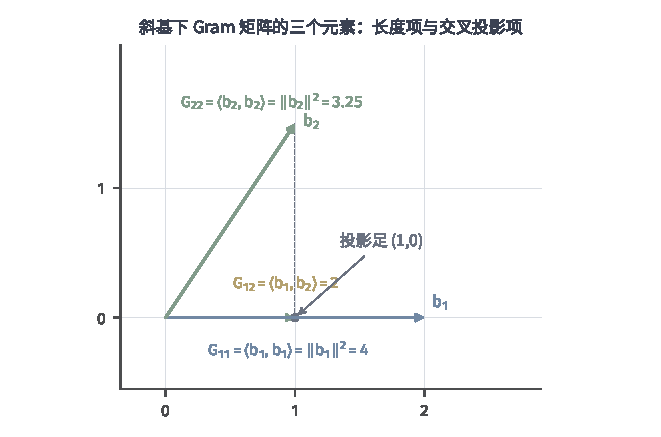
\includegraphics[width=112mm]{figures/01-mathematical-preliminaries-upper/03-linear-spaces/matplotlib/ls-gram-matrix-coefficients/ls-gram-matrix-coefficients.pdf}
  \caption{Gram矩阵把一组基向量的两两内积排成数表。左：平面上两条不垂直的基向量$\bm b_1,\bm b_2$及其夹角；右：$G_{i,j}=\langle\bm b_i,\bm b_j\rangle$构成的$2\times2$Gram矩阵，对角元为各向量长度平方，非对角元为夹角投影。基越接近正交，非对角元越接近零；两向量共线时，某个非零组合的平方长度为零，Gram矩阵不再正定。向量与矩阵均为解析教学例。}
  \label{fig:ls-gram-matrix-coefficients}
\end{figure}

近共线在Gram矩阵上怎样表现？
\begin{example}[近共线两列的Gram矩阵]
\label{ex:ls-nearly-collinear-gram}
给定：贯穿例的两列$\bm c_1,\bm c_2$，取欧氏内积。

计算：由示例~\ref{ex:ls-nearly-collinear-angle}中的三个内积，
\[
 \bm G=\bm X_\varepsilon^\top\bm X_\varepsilon=\begin{bmatrix}3&3\\3&3+2\varepsilon^2\end{bmatrix},
 \qquad
 \bm a^\top\bm G\bm a=3(a_1+a_2)^2+2\varepsilon^2a_2^2 .
\]
$\varepsilon\neq0$时，二次型只在$a_1=a_2=0$时为零，所以$\bm G$正定。取$\bm a=(1,-1)^\top$，二次型只有$2\varepsilon^2$；对应的组合$\bm c_1-\bm c_2=-\varepsilon\bm q$确实很短。

结论：$\bm G$正定，与两列线性无关一致；但存在系数使二次型接近零。近共线在Gram矩阵上表现为“正定但几乎退化”。
\end{example}

\paragraph{Gram因子定理}
Gram矩阵总是半正定的。反过来，每个半正定矩阵是否都是某组向量的Gram矩阵？关键是把半正定矩阵写成欧氏平方和，这一分解也说明加权配对不必当作新的几何。
\begin{theorem}[半正定矩阵的配方因子]
\label{thm:ls-gram-factor}
设$\bm M\in\mathbb R^{r\times r}$对称半正定，则存在$\bm L\in\mathbb R^{r\times r}$使$\bm M=\bm L^\top\bm L$；若$\bm M$正定，可取$\bm L$可逆。
\end{theorem}
\begin{proof}
对$r$归纳。$r=1$时$\bm M=(m_{1,1})$且$m_{1,1}\geq0$，取$\bm L=(\sqrt{m_{1,1}})$即可。

设$r>1$。若所有对角元都为零，任取$i\neq j$，把$\bm x=\bm e_i+t\bm e_j$代入半正定性：
\[
 0\leq\bm x^\top\bm M\bm x=m_{i,i}+2t\,m_{i,j}+t^2m_{j,j}=2t\,m_{i,j},
\]
对正负$t$同时成立迫使$m_{i,j}=0$，于是$\bm M=\bm0$，取$\bm L=\bm0$。

否则存在正的对角元。取一个置换矩阵$\bm P$把它换到首位（行列同步交换）；$\bm P$的各列是互不相同的标准坐标向量，所以$\bm P^\top\bm P=\bm P\bm P^\top=\bm I$。记
\[
 \widetilde{\bm M}=\bm P\bm M\bm P^\top
 =\begin{bmatrix}a&\bm b^\top\\ \bm b&\bm C\end{bmatrix},\qquad a>0.
\]
$\widetilde{\bm M}$仍对称半正定，因为$\bm x^\top\widetilde{\bm M}\bm x=(\bm P^\top\bm x)^\top\bm M(\bm P^\top\bm x)\geq0$。对第一个变量配方：令$\bm x=(-\bm b^\top\bm u/a,\bm u)$，展开得$\bm x^\top\widetilde{\bm M}\bm x=\bm u^\top(\bm C-\bm b\bm b^\top/a)\bm u\geq0$，故余项$\bm M'=\bm C-\bm b\bm b^\top/a$仍半正定。由归纳假设$\bm M'=\bm L'^\top\bm L'$，取上三角因子
\[
 \widetilde{\bm L}=\begin{bmatrix}\sqrt a&\bm b^\top/\sqrt a\\ \bm0&\bm L'\end{bmatrix},
\]
按分块乘法直接相乘得
\[
 \widetilde{\bm L}^\top\widetilde{\bm L}
 =\begin{bmatrix}a&\bm b^\top\\ \bm b&\bm b\bm b^\top/a+\bm L'^\top\bm L'\end{bmatrix}
 =\widetilde{\bm M}.
\]
换回原矩阵：$\bm M=\bm P^\top\widetilde{\bm M}\bm P=(\widetilde{\bm L}\bm P)^\top(\widetilde{\bm L}\bm P)$，取$\bm L=\widetilde{\bm L}\bm P$即可。

正定时$\bm M'$也正定（上述$\bm x$在$\bm u\neq\bm0$时非零），归纳得$\bm L'$可逆。分块上三角矩阵$\widetilde{\bm L}$的对角块$\sqrt a$与$\bm L'$都可逆，按分块乘法可以直接验证
\[
 \begin{bmatrix}1/\sqrt a&-\bm b^\top\bm L'^{-1}/a\\ \bm0&\bm L'^{-1}\end{bmatrix}
\]
是它的逆，于是$\bm L=\widetilde{\bm L}\bm P$作为可逆矩阵的乘积仍可逆。
\end{proof}
下面对一个二阶正定矩阵按证明的步骤求出因子。
\begin{example}[二阶正定矩阵的配方因子]
\label{ex:ls-gram-factor-two-by-two}
给定：$\bm M=\left[\begin{smallmatrix}4&2\\2&2\end{smallmatrix}\right]$。

计算：首个对角元$a=4>0$，不需要置换；$\bm b=(2)$，余项$\bm M'=2-2^2/4=1$，取$\bm L'=(1)$。按证明中的分块形式，
\[
 \bm L=\begin{bmatrix}\sqrt a&\bm b^\top/\sqrt a\\ 0&\bm L'\end{bmatrix}=\begin{bmatrix}2&1\\0&1\end{bmatrix}.
\]
直接验证：$\bm L^\top\bm L=\left[\begin{smallmatrix}2&0\\1&1\end{smallmatrix}\right]\left[\begin{smallmatrix}2&1\\0&1\end{smallmatrix}\right]=\left[\begin{smallmatrix}4&2\\2&2\end{smallmatrix}\right]=\bm M$。相应地，
\[
 \bm x^\top\bm M\bm x=4x_1^2+4x_1x_2+2x_2^2=(2x_1+x_2)^2+x_2^2 .
\]

结论：$\bm M=\bm L^\top\bm L$，且$\bm L$可逆；二次型被写成两个平方之和。
\end{example}
于是正定矩阵给出的加权长度可写成$\lVert\bm x\rVert_{\bm M}=\lVert\bm L\bm x\rVert_2$：加权内积只是把$\bm x$换成新坐标$\bm L\bm x$再量欧氏长度。证明中的配方步骤就是第~\ref{sec:ls-exact-linear-equations}节Cholesky分解的雏形。

\paragraph{半正定矩阵与Gram矩阵}
Gram矩阵总是半正定的；反过来，每个半正定矩阵都是某组向量的Gram矩阵。由定理~\ref{thm:ls-gram-factor}，半正定的$\bm M$可写成$\bm M=\bm L^\top\bm L$，记$\bm l_i$为$\bm L$的第$i$列，则$m_{i,j}=\bm l_i^\top\bm l_j=\langle\bm l_i,\bm l_j\rangle$，$\bm M$正是$\bm l_1,\ldots,\bm l_r$在欧氏内积下的Gram矩阵。所以“半正定”与“是一组向量的两两内积”说的是同一件事，判断一个矩阵半正定，可以去找这样一组向量。

这一观点给出一个关于逐元素乘积（第~\ref{sec:ls-hadamard-product}节）的结论：两个半正定矩阵的逐元素乘积仍半正定吗？设$\bm A,\bm B$均为$n$阶半正定矩阵。由定理~\ref{thm:ls-gram-factor}，$\bm A=\bm U^\top\bm U$、$\bm B=\bm V^\top\bm V$；记$\bm u_i,\bm v_i$分别为$\bm U,\bm V$的第$i$列，则$A_{i,k}=\langle\bm u_i,\bm u_k\rangle$、$B_{i,k}=\langle\bm v_i,\bm v_k\rangle$。考虑二阶数组$\bm u_1\otimes\bm v_1,\ldots,\bm u_n\otimes\bm v_n$，由Frobenius内积下张量积配对的分离性（第~\ref{sec:ls-tensor-operation-properties}节），它们的Gram矩阵为
\[
 \langle\bm u_i\otimes\bm v_i,\bm u_k\otimes\bm v_k\rangle_{\mathrm F}
 =\langle\bm u_i,\bm u_k\rangle\langle\bm v_i,\bm v_k\rangle
 =A_{i,k}B_{i,k}.
\]
Gram矩阵恒半正定，故逐元素乘积$\bm A\odot\bm B$半正定，这就是\term{Schur乘积}定理（Schur product theorem）。下面用一个二阶例子核对。
\begin{example}[两个半正定矩阵的逐元素乘积]
\label{ex:ls-schur-product}
给定：$\bm A=\bm B=\left[\begin{smallmatrix}1&1\\1&2\end{smallmatrix}\right]$。

计算：$\bm A$的二次型为$x_1^2+2x_1x_2+2x_2^2=(x_1+x_2)^2+x_2^2\geq0$，所以$\bm A$半正定。逐元素乘积及其二次型为
\[
 \bm A\odot\bm B=\begin{bmatrix}1&1\\1&4\end{bmatrix},
 \qquad
 x_1^2+2x_1x_2+4x_2^2=(x_1+x_2)^2+3x_2^2\geq0 .
\]

结论：$\bm A\odot\bm B$仍半正定，与Schur乘积定理一致。
\end{example}
核方法中两个核矩阵的逐元素乘积仍是合法的核矩阵，依据就是这一定理。

\paragraph{坐标下的内积}
选定基以后，一般内积空间上的内积也由一张矩阵完全确定，这张矩阵就是基的Gram矩阵。设$\mathcal B=(\bm b_1,\ldots,\bm b_d)$是$V$的基，$\bm G$是它的Gram矩阵。对$\bm v=\sum_ix_i\bm b_i$、$\bm w=\sum_jy_j\bm b_j$，按双线性展开得
\[
 \langle\bm v,\bm w\rangle=\sum_{i,j}x_iy_j\langle\bm b_i,\bm b_j\rangle=[\bm v]_{\mathcal B}^\top\,\bm G\,[\bm w]_{\mathcal B}.
\]
基线性无关，所以$\bm G$对称正定：在坐标下，任一内积都是以$\bm G$为权重的加权内积。特别地，$\mathbb R^d$上的任一内积在标准基下都是$\bm x^\top\bm G\bm y$，其中$g_{i,j}=\langle\bm e_i,\bm e_j\rangle$；反过来，每个对称正定矩阵都给出一个加权内积。所以$\mathbb R^d$上的内积与$d$阶对称正定矩阵一一对应，欧氏内积对应$\bm I$。下面用示例~\ref{ex:ls-two-point-inner-product}的内积核对坐标公式。
\begin{example}[两点内积的坐标计算]
\label{ex:ls-two-point-inner-product-coordinates}
给定：示例~\ref{ex:ls-two-point-inner-product}中$P_1$上的内积$\langle f,g\rangle=f(0)g(0)+f(1)g(1)$，基$(1,t)$，以及$f=1+t$、$g=1-2t$。

计算：由$\langle1,1\rangle=1\cdot1+1\cdot1=2$、$\langle1,t\rangle=1\cdot0+1\cdot1=1$、$\langle t,t\rangle=0\cdot0+1\cdot1=1$，基的Gram矩阵为
\[
 \bm G=\begin{bmatrix}2&1\\1&1\end{bmatrix}.
\]
按定义，$f$在$t=0,1$处取值$1,2$，$g$取值$1,-1$，所以$\langle f,g\rangle=1\cdot1+2\cdot(-1)=-1$。按坐标，$[f]=(1,1)^\top$、$[g]=(1,-2)^\top$，
\[
 (1,1)\,\bm G\begin{bmatrix}1\\-2\end{bmatrix}=(3,2)\begin{bmatrix}1\\-2\end{bmatrix}=-1 .
\]

结论：两种算法给出同一个内积值$-1$。
\end{example}
若基两两正交且长度为$1$，则$\bm G=\bm I$，内积在坐标下就是欧氏内积；这样的基是第~\ref{sec:ls-orthonormal-bases}节的主题。

\subsection{子空间之间的正交}
\label{sec:ls-orthogonality}

Gram矩阵记录的是一组向量两两之间是否正交。本小节把正交推广为一个向量与整个子空间的正交，得到由内积唯一确定的补空间，并据此证明四个基本子空间之间的垂直关系。

\paragraph{正交补}
第~\ref{sec:ls-direct-sum}节说明，一个子空间的补空间一般不唯一。有了内积，是否存在一个由“垂直”唯一确定的补空间？设$U$是有限维内积空间$V$的子空间，与$U$中每个向量都正交的向量组成的集合
\[
 U^\perp=\{\bm r\in V:\langle\bm u,\bm r\rangle=0,\ \forall\bm u\in U\}
\]
称为$U$的\term{正交补}（orthogonal complement）。由内积的双线性，$U^\perp$对线性组合封闭，是子空间。要检查$\bm r\in U^\perp$，只需检查它与$U$的一组基逐个正交，因为与基向量都正交的向量与基向量的每个组合也正交。

\paragraph{正交直和}
正交补确实是一个补空间，而且分解可以由Gram矩阵算出。
\begin{lemma}[正交直和]
\label{lem:ls-orthogonal-decomposition}
设$U$是有限维内积空间$V$的子空间，则每个$\bm x\in V$唯一分解为$\bm x=\bm u+\bm r$，其中$\bm u\in U$、$\bm r\in U^\perp$；即$V=U\oplus U^\perp$。
\end{lemma}
\begin{proof}
取$U$的一组基$\bm b_1,\ldots,\bm b_r$，它线性无关，所以Gram矩阵$\bm G$正定，从而可逆。对任意$\bm x$，令$\bm u=\sum_j a_j\bm b_j$，并要求$\bm r=\bm x-\bm u$与每个$\bm b_i$正交，得到系数方程
\[
 \sum_j g_{i,j}a_j=\langle\bm b_i,\bm x\rangle,\qquad i=1,\ldots,r,
\]
即$\bm G\bm a=(\langle\bm b_i,\bm x\rangle)_i$。可逆的$\bm G$保证系数唯一解出，残差$\bm r$与全部基向量正交，因而落在$U^\perp$。

若$\bm x=\bm u+\bm r=\bm u'+\bm r'$是两种分解，则$\bm u-\bm u'=\bm r'-\bm r$同时属于$U$与$U^\perp$，与自身正交，长度为零，故两种分解相同。
\end{proof}
所以正交补是$U$的一个补空间，并且由内积唯一确定，称$V=U\oplus U^\perp$为正交直和；由维数公式，$\dim U^\perp=\dim V-\dim U$。下面在$\mathbb R^3$中做一次分解。
\begin{example}[向一条直线的正交分解]
\label{ex:ls-orthogonal-decomposition-line}
给定：$\mathbb R^3$取欧氏内积，$U=\operatorname{span}\{\bm c_1\}$，$\bm c_1=(1,1,1)^\top$，$\bm y=(1,1.1,0.9)^\top$。

计算：$U^\perp$由与$\bm c_1$正交的向量组成，即坐标和为零的平面。$U$只有一个基向量，Gram方程只有一个未知数：$\langle\bm c_1,\bm c_1\rangle a=\langle\bm c_1,\bm y\rangle$，即$3a=3$，所以$a=1$。于是
\[
 \bm u=\bm c_1=(1,1,1)^\top,
 \qquad
 \bm r=\bm y-\bm u=(0,0.1,-0.1)^\top,
\]
$\bm r$的坐标和为零，确实属于$U^\perp$。

结论：$\bm y=\bm u+\bm r$就是$\bm y$在正交直和$\mathbb R^3=U\oplus U^\perp$中的分解。
\end{example}
这里只证明正交分量存在且唯一；它就是$U$中离$\bm x$最近的点，这一判定与具体算法在第~\ref{sec:ls-subspace-nearest-points}节给出。

取两次正交补会回到原来的子空间：$(U^\perp)^\perp=U$。一方面，$U$中每个向量与$U^\perp$中每个向量正交，所以$U\subseteq(U^\perp)^\perp$；另一方面，对$U^\perp$用上面的维数关系，$\dim(U^\perp)^\perp=\dim V-\dim U^\perp=\dim U$。包含且同维，由第~\ref{sec:ls-dimension}节两者相等。

\paragraph{四个基本子空间的正交关系}
示例~\ref{ex:ls-rank-one-four-subspaces}显示，行空间的方向与零空间垂直，列空间的方向与左零空间垂直。现在在$\mathbb R^d$与$\mathbb R^m$上取欧氏内积，证明这对任何矩阵都成立。
\begin{theorem}[四个基本子空间的正交关系]
\label{thm:ls-four-subspaces-orthogonality}
设$\bm A\in\mathbb R^{m\times d}$，$\mathbb R^d$与$\mathbb R^m$取欧氏内积。则
\begin{equation}
 \operatorname{null}(\bm A)=\operatorname{range}(\bm A^\top)^\perp,\qquad
 \operatorname{null}(\bm A^\top)=\operatorname{range}(\bm A)^\perp,
 \label{eq:ls-four-subspaces-orthogonality}
\end{equation}
因而有正交直和
\begin{equation}
 \mathbb R^d=\operatorname{range}(\bm A^\top)\oplus\operatorname{null}(\bm A),\qquad
 \mathbb R^m=\operatorname{range}(\bm A)\oplus\operatorname{null}(\bm A^\top).
 \label{eq:ls-four-subspaces-decomposition}
\end{equation}
\end{theorem}
\begin{proof}
由转置的乘积规则（第~\ref{sec:ls-reshaping}节），对任意$\bm x\in\mathbb R^d$、$\bm y\in\mathbb R^m$，
\[
 \langle\bm A\bm x,\bm y\rangle=(\bm A\bm x)^\top\bm y=\bm x^\top(\bm A^\top\bm y)=\langle\bm x,\bm A^\top\bm y\rangle.
\]
$\bm y\in\operatorname{range}(\bm A)^\perp$意味着左端对一切$\bm x$为零，即右端对一切$\bm x$为零；取$\bm x=\bm A^\top\bm y$可见这当且仅当$\bm A^\top\bm y=\bm0$。所以$\operatorname{range}(\bm A)^\perp=\operatorname{null}(\bm A^\top)$。把$\bm A$换成$\bm A^\top$得$\operatorname{range}(\bm A^\top)^\perp=\operatorname{null}(\bm A)$。正交直和由引理~\ref{lem:ls-orthogonal-decomposition}得到。
\end{proof}
两边再取正交补，并用$(U^\perp)^\perp=U$，还得到$\operatorname{null}(\bm A)^\perp=\operatorname{range}(\bm A^\top)$、$\operatorname{null}(\bm A^\top)^\perp=\operatorname{range}(\bm A)$。于是输入空间分成两块互相垂直的部分：零空间是被$\bm A$消去的方向，行空间是真正影响输出的方向；输出空间也分成两块：列空间是可达的输出，左零空间是无论如何都到达不了的方向。

这一定理与第~\ref{sec:ls-kernel-image}节的维数关系相互印证。由正交直和与秩零度定理分别得到
\[
 d=\dim\operatorname{range}(\bm A^\top)+\dim\operatorname{null}(\bm A),\qquad
 d=\operatorname{rank}\bm A+\dim\operatorname{null}(\bm A).
\]
两式比较，又一次得到行秩等于列秩。示例~\ref{ex:ls-rank-one-four-subspaces}中逐项相乘再相加得零的观察，现在由定理得到了解释。

输出端的分解给出方程$\bm A\bm x=\bm b$有解的一个判据：$\bm b\in\operatorname{range}(\bm A)$当且仅当$\bm b$与左零空间中每个向量正交。第~\ref{chap:linear-equations-and-optimization}章判断方程是否有解时会用到这一点。

\subsection{标准正交基的定义和性质}
\label{sec:ls-orthonormal-bases}

正交直和的证明要解Gram方程$\bm G\bm a=(\langle\bm b_i,\bm x\rangle)_i$，坐标下的内积要乘Gram矩阵，示例~\ref{ex:ls-coordinate-instability}还显示，接近共线的基会把小的对象记成很大的系数。这些麻烦都来自基向量之间的相互干扰，即Gram矩阵的非对角元。本小节定义消除这种干扰的基，证明它确实是一组基，再依次给出它下的坐标、它们之间的换基，以及向子空间的正交分解。

\paragraph{标准正交基的定义}
一组向量$\bm q_1,\ldots,\bm q_r$若满足
\[
 \langle\bm q_i,\bm q_j\rangle=\delta_{i,j}=\begin{cases}1,&i=j,\\0,&i\neq j,\end{cases}
\]
即两两正交且长度都为$1$，就称为标准正交组；它的Gram矩阵是$\bm I_r$。张成子空间$U$的标准正交组称为$U$的\term{标准正交基}（orthonormal basis）；$U=V$时就是$V$的标准正交基。

在$\mathbb R^m$中取欧氏内积，把$r$个向量排成$\bm Q\in\mathbb R^{m\times r}$的各列，它们的Gram矩阵是$\bm Q^\top\bm Q$，所以标准正交的条件就是$\bm Q^\top\bm Q=\bm I_r$。$r=m$时$\bm Q$是第~\ref{sec:ls-orthogonal-matrices}节的正交矩阵；$r<m$时$\bm Q^\top\bm Q=\bm I_r$仍成立，但$\bm Q\bm Q^\top$的秩只有$r$，不等于$\bm I_m$，$\bm Q$只有左逆$\bm Q^\top$。

\paragraph{标准正交组构成基}
标准正交组总是线性无关。设$\sum_jc_j\bm q_j=\bm0$，两边与$\bm q_i$作内积，左边每一项$c_j\langle\bm q_j,\bm q_i\rangle$只在$j=i$时不为零，于是$c_i=0$；$i$任意，所以全部系数为零。同样的论证说明两两正交的非零向量组线性无关，只是最后一步改为由$c_i\langle\bm q_i,\bm q_i\rangle=0$与$\langle\bm q_i,\bm q_i\rangle>0$得$c_i=0$。因此标准正交组是它所张成子空间的一组基；$d$维内积空间中$d$个两两正交的单位向量个数等于维数，自动构成整个空间的标准正交基，不必另行验证张成。$\mathbb R^d$的标准基在欧氏内积下是标准正交基；$\bm q_1=(1,1)^\top/\sqrt2$、$\bm q_2=(1,-1)^\top/\sqrt2$是$\mathbb R^2$的另一组标准正交基。

\paragraph{标准正交基下的坐标}
在标准正交基下，坐标不必解方程。若$\bm v=\sum_jc_j\bm q_j$，两边与$\bm q_i$作内积，右边只剩$c_i$一项，所以
\begin{equation}
 \bm v=\sum_{j=1}^d\langle\bm v,\bm q_j\rangle\,\bm q_j.
 \label{eq:ls-orthonormal-expansion}
\end{equation}
每个系数只与自己的方向有关，增加或删去其他方向都不改变它。坐标下的内积变成欧氏内积：$\langle\bm v,\bm w\rangle=\sum_jc_jd_j$，其中$c_j,d_j$分别是$\bm v,\bm w$的坐标；特别地
\begin{equation}
 \lVert\bm v\rVert^2=\sum_{j=1}^d\langle\bm v,\bm q_j\rangle^2,
 \label{eq:ls-parseval}
\end{equation}
长度的平方等于各坐标的平方和，称为Parseval恒等式，是勾股定理在$d$个互相垂直方向上的推广。下面用平面上的一组标准正交基验证这两点。
\begin{example}[标准正交基下的坐标与Parseval恒等式]
\label{ex:ls-orthonormal-coordinates}
给定：$\mathbb R^2$的标准正交基$\bm q_1=(1,1)^\top/\sqrt2$、$\bm q_2=(1,-1)^\top/\sqrt2$，向量$\bm v=(3,1)^\top$。

计算：由式~\eqref{eq:ls-orthonormal-expansion}，坐标为$\langle\bm v,\bm q_1\rangle=4/\sqrt2=2\sqrt2$与$\langle\bm v,\bm q_2\rangle=2/\sqrt2=\sqrt2$，不必解方程。坐标的平方和为$8+2=10$，而$\lVert\bm v\rVert^2=3^2+1^2=10$。

结论：坐标由内积直接读出，平方和等于长度的平方。
\end{example}
在标准正交基下，坐标的大小如实反映对象的大小，近共线基下“小对象、大系数”的现象不会发生。

\paragraph{标准正交基之间的换基}
设$\mathcal B=(\bm b_1,\ldots,\bm b_d)$与$\mathcal C$都是$V$的标准正交基，换基矩阵$\bm S=\bm S_{\mathcal C\leftarrow\mathcal B}$的第$j$列是$\bm b_j$的$\mathcal C$坐标。在标准正交基$\mathcal C$下内积就是坐标的欧氏内积，所以$\bm S$的第$i$、$j$两列的欧氏内积等于$\langle\bm b_i,\bm b_j\rangle=\delta_{i,j}$，即$\bm S^\top\bm S=\bm I$：两组标准正交基之间的换基矩阵是正交矩阵。

于是反向换基只需转置，$\bm S^{-1}=\bm S^\top$，不会出现示例~\ref{ex:ls-nearly-collinear-change-of-basis}中除以小数$\varepsilon$的放大。例如从上面的$(\bm q_1,\bm q_2)$换到标准基，换基矩阵的两列就是$\bm q_1,\bm q_2$本身。对线性算子，若只在标准正交基之间换基，相似关系$\bm B=\bm P^{-1}\bm A\bm P$变成$\bm B=\bm P^\top\bm A\bm P$；第~\ref{chap:linear-analysis}章的谱定理正是要在这一受限的换基下化简对称矩阵。

\paragraph{向子空间的正交分解}
若$\bm q_1,\ldots,\bm q_r$是子空间$U$的标准正交基，第~\ref{sec:ls-orthogonality}节正交直和中的Gram方程变成$\bm a=(\langle\bm q_i,\bm x\rangle)_i$，分解直接写出：
\begin{equation}
 \bm x=\underbrace{\sum_{j=1}^r\langle\bm x,\bm q_j\rangle\bm q_j}_{\bm u\in U}+\underbrace{\Bigl(\bm x-\sum_{j=1}^r\langle\bm x,\bm q_j\rangle\bm q_j\Bigr)}_{\bm r\in U^\perp}.
 \label{eq:ls-orthonormal-projection}
\end{equation}
$\bm u$称为$\bm x$在$U$上的正交投影。$\bm u$与$\bm r$正交，由勾股定理$\lVert\bm x\rVert^2=\lVert\bm u\rVert^2+\lVert\bm r\rVert^2\geq\sum_{j=1}^r\langle\bm x,\bm q_j\rangle^2$：沿一部分标准正交方向读出的系数平方和不超过总长度的平方，等号恰在$\bm x\in U$时成立。下面用这一公式重算示例~\ref{ex:ls-orthogonal-decomposition-line}中的分解。
\begin{example}[用标准正交基重算正交分解]
\label{ex:ls-orthonormal-projection-line}
给定：$U=\operatorname{span}\{\bm q_1\}$，$\bm q_1=(1,1,1)^\top/\sqrt3$，$\bm y=(1,1.1,0.9)^\top$。

计算：$\langle\bm y,\bm q_1\rangle=3/\sqrt3=\sqrt3$，投影为$\sqrt3\,\bm q_1=(1,1,1)^\top$，余量为$(0,0.1,-0.1)^\top$，它与$\bm q_1$正交。

结论：结果与示例~\ref{ex:ls-orthogonal-decomposition-line}相同，但这里不需要解Gram方程。
\end{example}
下一小节构造标准正交基，靠的正是这一公式。

\subsection{标准正交基的构建}
\label{sec:ls-orthonormal-basis-construction}

标准正交基如此方便，它是否总存在？给定任意一组基，怎样把它改造成标准正交基？上一小节的正交分解给出了思路：依次处理基向量，从每个向量中扣除它在已经造好的方向上的分量，剩下的部分与这些方向都垂直，再把它缩放到单位长度。本小节先给出这一过程并证明它总能完成，再把它在$\mathbb R^m$中写成矩阵分解，最后处理各列线性相关的情形。

\subsubsection{Gram--Schmidt正交化}

这一过程称为\term{Gram--Schmidt正交化}（Gram--Schmidt orthogonalization），也称施密特正交化。设$\bm v_1,\ldots,\bm v_k$线性无关。令$\bm u_1=\bm v_1$、$\bm q_1=\bm u_1/\lVert\bm u_1\rVert$；对$j=2,\ldots,k$依次令
\begin{equation}
 \bm u_j=\bm v_j-\sum_{i=1}^{j-1}\langle\bm v_j,\bm q_i\rangle\bm q_i,
 \qquad
 \bm q_j=\frac{\bm u_j}{\lVert\bm u_j\rVert}.
 \label{eq:ls-gram-schmidt}
\end{equation}
按式~\eqref{eq:ls-orthonormal-projection}，$\bm u_j$正是$\bm v_j$在$\operatorname{span}\{\bm q_1,\ldots,\bm q_{j-1}\}$的正交补中的分量。
\begin{theorem}[Gram--Schmidt正交化]
\label{thm:ls-gram-schmidt}
上述过程中每个$\bm u_j\neq\bm0$，得到的$\bm q_1,\ldots,\bm q_k$两两正交、长度为$1$，并且对每个$j$都有$\operatorname{span}\{\bm q_1,\ldots,\bm q_j\}=\operatorname{span}\{\bm v_1,\ldots,\bm v_j\}$。
\end{theorem}
\begin{proof}
对$j$归纳。$j=1$时$\bm u_1=\bm v_1\neq\bm0$，结论成立。设结论对$j-1$成立。对$i<j$，由$\bm q_1,\ldots,\bm q_{j-1}$两两正交且长度为$1$，
\[
 \langle\bm u_j,\bm q_i\rangle=\langle\bm v_j,\bm q_i\rangle-\langle\bm v_j,\bm q_i\rangle\langle\bm q_i,\bm q_i\rangle=0,
\]
所以$\bm u_j$与前面的方向都正交。若$\bm u_j=\bm0$，则$\bm v_j$属于$\operatorname{span}\{\bm q_1,\ldots,\bm q_{j-1}\}=\operatorname{span}\{\bm v_1,\ldots,\bm v_{j-1}\}$，与线性无关矛盾；故$\bm u_j\neq\bm0$，$\bm q_j$有定义且长度为$1$。最后，$\bm q_j$是$\bm v_j$与$\bm q_1,\ldots,\bm q_{j-1}$的组合，因而属于$\operatorname{span}\{\bm v_1,\ldots,\bm v_j\}$；反过来由式~\eqref{eq:ls-gram-schmidt}，$\bm v_j=\lVert\bm u_j\rVert\bm q_j+\sum_{i<j}\langle\bm v_j,\bm q_i\rangle\bm q_i$属于$\operatorname{span}\{\bm q_1,\ldots,\bm q_j\}$。两个张成空间互相包含，因而相等。
\end{proof}
对有限维内积空间的任意一组基作Gram--Schmidt正交化，就得到一组标准正交基，所以\emph{每个有限维内积空间都有标准正交基}。若已有几个两两正交的单位向量，先把它们扩充成一组基，再从它们之后开始正交化：前面的向量在过程中保持不变，所以任何标准正交组都能扩充成标准正交基。张成空间逐段相等也有用处：前$j$个新方向与前$j$个旧方向张成同一个子空间，正交化只是在每一段内部换了一组更好用的基。

\paragraph{算例}
标准正交基依赖内积，换一个内积，同一组基正交化的结果也不同。下面在示例~\ref{ex:ls-two-point-inner-product}的内积下对基$(1,t)$作正交化；在这个内积下$\langle1,t\rangle=1\neq0$，两个基向量并不正交。
\begin{example}[两点内积下的Gram--Schmidt正交化]
\label{ex:ls-gram-schmidt-two-point}
给定：$P_1$上的内积$\langle f,g\rangle=f(0)g(0)+f(1)g(1)$，基$(1,t)$。

计算：第一步，归一化第一个基向量。$\lVert1\rVert^2=1^2+1^2=2$，所以
\[
 q_1=\frac1{\sqrt2}.
\]

第二步，从第二个基向量中扣除它在$q_1$上的分量。$\langle t,q_1\rangle=\bigl(0\cdot1+1\cdot1\bigr)/\sqrt2=1/\sqrt2$，所以
\[
 u_2=t-\langle t,q_1\rangle q_1=t-\frac1{\sqrt2}\cdot\frac1{\sqrt2}=t-\frac12.
\]

第三步，归一化。$u_2$在$t=0,1$处的取值为$-\tfrac12,\tfrac12$，所以$\lVert u_2\rVert^2=\tfrac14+\tfrac14=\tfrac12$，
\[
 q_2=\frac{u_2}{\lVert u_2\rVert}=\sqrt2\Bigl(t-\frac12\Bigr).
\]

第四步，核对。$q_1$在$t=0,1$处取值都是$\tfrac1{\sqrt2}$，$q_2$取值为$-\tfrac{\sqrt2}2,\tfrac{\sqrt2}2$，所以$\langle q_1,q_2\rangle=\tfrac1{\sqrt2}\cdot\bigl(-\tfrac{\sqrt2}2\bigr)+\tfrac1{\sqrt2}\cdot\tfrac{\sqrt2}2=0$，$\lVert q_2\rVert^2=\tfrac12+\tfrac12=1$。

第五步，用新基读坐标。$f=1+t$在$t=0,1$处取值为$1,2$，所以$\langle f,q_1\rangle=(1+2)/\sqrt2=3/\sqrt2$，$\langle f,q_2\rangle=1\cdot\bigl(-\tfrac{\sqrt2}2\bigr)+2\cdot\tfrac{\sqrt2}2=\tfrac{\sqrt2}2$。还原得$\tfrac3{\sqrt2}\cdot\tfrac1{\sqrt2}+\tfrac{\sqrt2}2\cdot\sqrt2(t-\tfrac12)=\tfrac32+t-\tfrac12=1+t$。Parseval恒等式也成立：$\lVert f\rVert^2=1^2+2^2=5$，而$\tfrac92+\tfrac12=5$。

结论：$q_1=1/\sqrt2$、$q_2=\sqrt2(t-\tfrac12)$是这一内积下$P_1$的标准正交基，$1+t$在其下的坐标为$(3/\sqrt2,\ \sqrt2/2)$。
\end{example}
正交化把$t$换成了$t-\tfrac12$。在系数向量的欧氏内积下，$1$与$t$的系数列$(1,0)^\top$、$(0,1)^\top$本来就正交；换了内积以后，却需要这一步。

\subsubsection{QR分解}

在$\mathbb R^m$中取欧氏内积，Gram--Schmidt正交化可以写成一个矩阵等式，它把一组列向量的方向与组合系数分开记录。设$\bm A\in\mathbb R^{m\times d}$的列$\bm a_1,\ldots,\bm a_d$线性无关，对它们作正交化（即取$\bm v_j=\bm a_j$）。把式~\eqref{eq:ls-gram-schmidt}反过来写，$\bm a_j=\lVert\bm u_j\rVert\bm q_j+\sum_{i<j}\langle\bm a_j,\bm q_i\rangle\bm q_i$，即每一列只用到前$j$个正交方向：
\[
 \bm a_j=\sum_{i\leq j}r_{i,j}\bm q_i,\qquad
 r_{i,j}=\langle\bm a_j,\bm q_i\rangle\ (i<j),\qquad r_{j,j}=\lVert\bm u_j\rVert>0 .
\]
把$\bm q_1,\ldots,\bm q_d$排成$\bm Q\in\mathbb R^{m\times d}$，把系数$r_{i,j}$排成$d$阶上三角矩阵$\bm R$（$i>j$时$r_{i,j}=0$），按矩阵乘积的列读法，各列的这些关系合写为经济型\term{QR分解}（QR factorization）
\begin{equation}
 \bm A=\bm Q\bm R,\qquad
 \bm Q^\top\bm Q=\bm I_d,\quad\bm R\text{ 上三角且对角元为正}.
 \label{eq:ls-qr-factorization}
\end{equation}
由定理~\ref{thm:ls-gram-schmidt}，$\bm Q$的列是列空间$\operatorname{range}(\bm A)$的标准正交基，$\bm R$的第$j$列记录$\bm a_j$在这组正交方向上的坐标；$\bm R$的对角元为正，所以$\bm R$可逆。图~\ref{fig:vol1-add-linear-qr-columns}给出最小的二维情形：保留第一条单位方向，从第二列减去它在第一方向上的分量，列空间不变，减去的部分记进$\bm R$。
\begin{figure}[!htb]
  \centering
  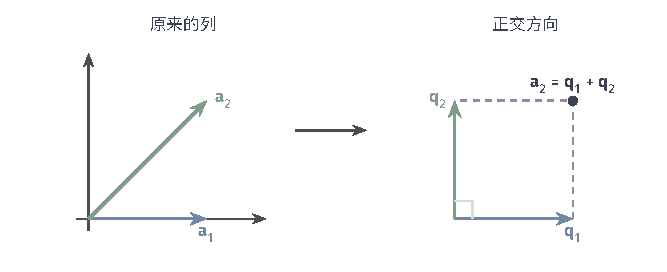
\includegraphics[width=112mm]{figures/01-mathematical-preliminaries-upper/03-linear-spaces/tikz/comprehension-additions/linear-qr-columns.pdf}
  \caption{QR把列的方向和组合系数分开。取$\bm a_1=(1,0)^\top$、$\bm a_2=(1,1)^\top$，
  正交化得到$\bm q_1=(1,0)^\top$、$\bm q_2=(0,1)^\top$，并有$\bm a_1=\bm q_1$、
  $\bm a_2=\bm q_1+\bm q_2$，故$\bm R=\left[\begin{smallmatrix}1&1\\0&1\end{smallmatrix}\right]$。
  虚线补出第二列的分量。}
  \label{fig:vol1-add-linear-qr-columns}
\end{figure}

这一分解的用处在于，涉及列空间的计算可以改在标准正交的$\bm Q$上进行，坐标由内积直接读出，不必再解Gram方程；第~\ref{chap:linear-equations-and-optimization}章解方程与最小二乘问题时正是这样使用它的。

\subsubsection{列相关时的处理}

定理~\ref{thm:ls-gram-schmidt}要求各列线性无关。若不满足，某一步会出现$\bm u_j=\bm0$：由式~\eqref{eq:ls-orthonormal-projection}，这恰好说明$\bm a_j$已在前面方向张成的空间中，没有带来新方向。这时不能对零向量归一化，应跳过这一列，只在$\bm R$中记下它的系数$\langle\bm a_j,\bm q_i\rangle$；跳过它不影响后续各列，因为张成的空间没有变。

全部处理完以后，留下的$\bm q$个数等于列空间的维数$r=\operatorname{rank}\bm A$，仍有$\bm A=\bm Q\bm R$，其中$\bm Q\in\mathbb R^{m\times r}$的列是列空间的标准正交基，$\bm R\in\mathbb R^{r\times d}$的各行从左到右第一个非零元的位置逐行右移；$r<d$时$\bm R$不是方阵，不能求逆。下面是最小的例子。
\begin{example}[列相关时跳过零余量]
\label{ex:ls-qr-dependent-columns}
给定：$\bm A=[\bm a_1\ \bm a_2]$，$\bm a_1=(1,0)^\top$、$\bm a_2=(2,0)^\top$。

计算：$\bm q_1=\bm a_1$。$\langle\bm a_2,\bm q_1\rangle=2$，扣除后$\bm u_2=\bm a_2-2\bm q_1=\bm0$，所以跳过$\bm a_2$，只在$\bm R$中记下系数$2$。于是$r=1$，
\[
 \bm Q=\begin{bmatrix}1\\0\end{bmatrix},\qquad
 \bm R=\begin{bmatrix}1&2\end{bmatrix},\qquad
 \bm Q\bm R=\begin{bmatrix}1&2\\0&0\end{bmatrix}=\bm A .
\]

结论：列空间仍是$x$轴，$\bm Q$的一列构成它的标准正交基，$\operatorname{rank}\bm A=1$。
\end{example}
于是在精确算术下，同一过程也给出列空间的一组标准正交基与矩阵的秩。有限精度下扣除后的余量很少恰好为零，怎样判断它“算作零”、怎样改写扣除顺序以减少正交性的损失，属于数值计算问题，在第~\ref{sec:ls-numerical-sensitivity}节讨论。

\subsection{伴随}
\label{sec:ls-adjoints}

第~\ref{sec:ls-dual-spaces}节的读取规则属于对偶空间，与被读取的向量不在同一个空间；转置在那里是对偶映射的矩阵。有了内积，读取可以写成与一个固定向量的配对，对偶映射也就变成内积空间之间的映射，称为伴随。第~\ref{sec:ls-orthogonality}节证明四个基本子空间的正交关系时，用到的正是它在欧氏内积下的形式：作用在左侧向量上的$\bm A$可以改写成作用在右侧向量上的$\bm A^\top$。第~\ref{chap:linear-analysis}章的对称矩阵与谱分解、第~\ref{chap:linear-equations-and-optimization}章的加权最小二乘，都要用到这种搬动。

\paragraph{线性泛函的内积表示}
\phantomsection
\label{sec:ls-riesz-representation}
在$\mathbb R^d$的欧氏内积下，加权读取$\varphi(\bm x)=\bm a^\top\bm x$就是与向量$\bm a$的内积。一般有限维内积空间中，每个读取也都能这样写。
\begin{theorem}[有限维Riesz表示定理]
\label{thm:ls-riesz-representation}
设$V$是有限维内积空间。对每个$\varphi\in V^*$，存在唯一的$\bm v_\varphi\in V$，使$\varphi(\bm x)=\langle\bm x,\bm v_\varphi\rangle$对所有$\bm x\in V$成立。
\end{theorem}
\begin{proof}
取$V$的一组标准正交基$\bm q_1,\ldots,\bm q_d$（第~\ref{sec:ls-orthonormal-basis-construction}节），令$\bm v_\varphi=\sum_j\varphi(\bm q_j)\bm q_j$。由式~\eqref{eq:ls-orthonormal-expansion}，$\bm x=\sum_j\langle\bm x,\bm q_j\rangle\bm q_j$，于是
\[
 \varphi(\bm x)=\sum_j\langle\bm x,\bm q_j\rangle\varphi(\bm q_j)=\Bigl\langle\bm x,\sum_j\varphi(\bm q_j)\bm q_j\Bigr\rangle=\langle\bm x,\bm v_\varphi\rangle.
\]
若$\bm v,\bm v'$都满足要求，则$\langle\bm x,\bm v-\bm v'\rangle=0$对一切$\bm x$成立，取$\bm x=\bm v-\bm v'$得$\bm v=\bm v'$。
\end{proof}
对应$\varphi\mapsto\bm v_\varphi$保持线性组合（由表示向量的唯一性），并且每个$\bm v$都表示读取$\langle\cdot,\bm v\rangle$，所以它是$V^*$到$V$的双射。在它之下，标准正交基的对偶基就是这组基本身，因为第$j$个坐标读取是$\bm x\mapsto\langle\bm x,\bm q_j\rangle$。对一般的基，对偶基对应的向量与原基不同：图~\ref{fig:ls-dual-basis-readout}中的红色箭头$\bm b^1,\bm b^2$正是对偶读取$\varphi_1,\varphi_2$在欧氏内积下对应的向量。

表示向量依赖内积，读取本身却不依赖。在$\mathbb R^d$上取加权内积$\langle\bm x,\bm y\rangle_{\bm M}=\bm x^\top\bm M\bm y$，同一个读取$\varphi(\bm x)=\bm a^\top\bm x=\bm x^\top\bm M(\bm M^{-1}\bm a)$对应的向量是$\bm M^{-1}\bm a$，而不是$\bm a$。函数空间中也是如此。
\begin{example}[积分读取在两点内积下的表示向量]
\label{ex:ls-riesz-integral-two-point}
给定：$P_1$上的内积$\langle f,g\rangle=f(0)g(0)+f(1)g(1)$与读取$\varphi(f)=\int_0^1f(t)\,\mathrm dt$。

计算：对$f=a+bt$，$\varphi(f)=a+b/2$。另一方面，$f$与常数函数$\tfrac12$的内积为
\[
 \Bigl\langle f,\tfrac12\Bigr\rangle=\tfrac12\bigl(f(0)+f(1)\bigr)=\tfrac12(a+a+b)=a+\frac b2 .
\]

结论：$\bm v_\varphi$是常数函数$\tfrac12$。这也说明梯形公式$\tfrac12\bigl(f(0)+f(1)\bigr)$对一次函数精确。
\end{example}
表示向量还给出读取的大小。由Cauchy--Schwarz不等式，$|\varphi(\bm x)|\leq\lVert\bm x\rVert\,\lVert\bm v_\varphi\rVert$；$\bm v_\varphi\neq\bm0$时取$\bm x=\bm v_\varphi/\lVert\bm v_\varphi\rVert$可取到等号，所以第~\ref{sec:ls-finite-dimensional-sequences}节定义的$\lVert\varphi\rVert_*$等于$\lVert\bm v_\varphi\rVert$。

\paragraph{伴随的定义}
对偶映射把输出端的读取$f$传回输入端，得到读取$f\circ T$。若把读取都换成表示它的向量，就得到下面的定义。设$T:V\to W$是两个有限维实内积空间之间的线性映射。若存在$T^\star:W\to V$使
\begin{equation}
 \langle T\bm x,\bm y\rangle_W=\langle\bm x,T^\star\bm y\rangle_V
 \label{eq:ls-adjoint-pairing}
\end{equation}
对所有$\bm x\in V$、$\bm y\in W$成立，则$T^\star$称为$T$的\term{伴随}（adjoint）。
\label{def:linear-algebra-adjoint}

伴随总存在且唯一。固定$\bm y\in W$，$\bm x\mapsto\langle T\bm x,\bm y\rangle_W$是$V$上的线性泛函，由定理~\ref{thm:ls-riesz-representation}，存在唯一的向量使它写成与该向量的内积，把这个向量记为$T^\star\bm y$。$T^\star$对$\bm y$线性：$\langle\bm x,aT^\star\bm y+bT^\star\bm y'\rangle_V=a\langle T\bm x,\bm y\rangle_W+b\langle T\bm x,\bm y'\rangle_W=\langle T\bm x,a\bm y+b\bm y'\rangle_W$，由表示向量的唯一性，$T^\star(a\bm y+b\bm y')=aT^\star\bm y+bT^\star\bm y'$。

用对偶映射的语言说，若把$\bm y\in W$看成读取$\langle\cdot,\bm y\rangle_W$，则$T'$把它送到读取$\langle T\,\cdot,\bm y\rangle_W=\langle\cdot,T^\star\bm y\rangle_V$：伴随就是借内积把读取换成向量以后的对偶映射。

具体计算时取$V,W$的基。由坐标下的内积公式，两边的内积写成$\langle\bm x,\bm x'\rangle_V=\bm x^\top\bm M_V\bm x'$、$\langle\bm y,\bm y'\rangle_W=\bm y^\top\bm M_W\bm y'$（这里$\bm x,\bm y$等指坐标），其中$\bm M_V,\bm M_W$是两组基的Gram矩阵，对称正定因而可逆；设$T$的矩阵为$\bm A$，伴随的矩阵为$\bm B$。式~\eqref{eq:ls-adjoint-pairing}要求$(\bm A\bm x)^\top\bm M_W\bm y=\bm x^\top\bm M_V\bm B\bm y$对所有$\bm x,\bm y$成立；取$\bm x,\bm y$为标准坐标向量逐个比较元素，这等价于$\bm A^\top\bm M_W=\bm M_V\bm B$，即
\begin{equation}
 \bm B=\bm M_V^{-1}\bm A^\top\bm M_W.
 \label{eq:ls-weighted-adjoint}
\end{equation}
两端都取标准正交基时，$\bm M_V,\bm M_W$都是单位矩阵，伴随矩阵就是$\bm A^\top$，与对偶映射的矩阵相同；两边权重不同时，伴随既不是单纯转置，也不是转置再求逆。下面的例子说明这一点。
\begin{example}[加权内积下的伴随]
\label{ex:ls-weighted-adjoint}
给定：$V=W=\mathbb R^2$都取加权内积$\langle\bm x,\bm y\rangle_{\bm M}=\bm x^\top\bm M\bm y$，$\bm M=\operatorname{diag}(4,1)$；$T\bm x=\bm A\bm x$，$\bm A=\left[\begin{smallmatrix}0&1\\0&0\end{smallmatrix}\right]$。

计算：由式~\eqref{eq:ls-weighted-adjoint}，
\[
 \bm B=\bm M^{-1}\bm A^\top\bm M
 =\begin{bmatrix}1/4&0\\0&1\end{bmatrix}\begin{bmatrix}0&0\\1&0\end{bmatrix}\begin{bmatrix}4&0\\0&1\end{bmatrix}
 =\begin{bmatrix}0&0\\4&0\end{bmatrix}.
\]
直接核对：$\bm A\bm x=(x_2,0)^\top$，$\langle\bm A\bm x,\bm y\rangle_{\bm M}=4x_2y_1$；$\bm B\bm y=(0,4y_1)^\top$，$\langle\bm x,\bm B\bm y\rangle_{\bm M}=x_2\cdot4y_1$，两者相等。

结论：伴随矩阵是$\left[\begin{smallmatrix}0&0\\4&0\end{smallmatrix}\right]$，而不是$\bm A^\top=\left[\begin{smallmatrix}0&0\\1&0\end{smallmatrix}\right]$。
\end{example}
对偶映射的矩阵总是$\bm A^\top$，差别来自读取与向量之间的对应$\bm a\mapsto\bm M^{-1}\bm a$随内积改变。四个基本子空间正交关系的证明只用到配对恒等式，所以对一般内积空间同样有$\ker T^\star=(\operatorname{im}T)^\perp$、$\ker T=(\operatorname{im}T^\star)^\perp$。

\paragraph{伴随的运算规则}
伴随与组合的规则由配对定义逐项推出：
\[
 (T+S)^\star=T^\star+S^\star,\qquad
 (cT)^\star=c\,T^\star,\qquad
 (TS)^\star=S^\star T^\star,\qquad
 T^{\star\star}=T.
\]
例如$\langle TS\bm x,\bm y\rangle=\langle S\bm x,T^\star\bm y\rangle=\langle\bm x,S^\star T^\star\bm y\rangle$，复合伴随的次序与乘积转置一样反转；恒等映射的伴随是自身。图~\ref{fig:ls-adjoint-action-transfer}把这种配对方向的搬回画成示意图。

伴随也不是逆：逆把输出复原成输入，伴随只把读取方向换一侧。
\begin{example}[反例：伴随不是逆]
\label{ex:ls-adjoint-not-inverse}
给定：非零内积空间$V$上的算子$T=2\operatorname{id}$。

验证：$\langle2\bm x,\bm y\rangle=\langle\bm x,2\bm y\rangle$对一切$\bm x,\bm y$成立，所以$T^\star=2\operatorname{id}$；而$T^{-1}=\tfrac12\operatorname{id}$。

结论：$T^\star\neq T^{-1}$。
\end{example}
\begin{figure}[!htb]
  \centering
  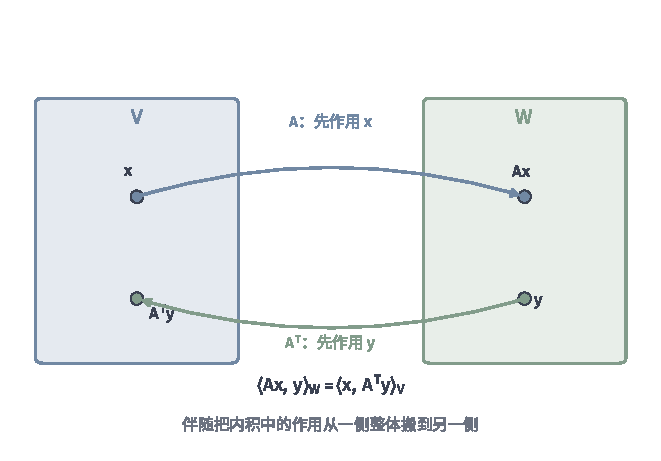
\includegraphics[width=112mm]{figures/01-mathematical-preliminaries-upper/03-linear-spaces/matplotlib/ls-adjoint-action-transfer/ls-adjoint-action-transfer.pdf}
  \caption{内积伴随把输出端的配对搬回输入端。左：$T:V\to W$把$\bm x$映成$T\bm x$，与$\bm y\in W$配对；右：伴随$T^\star:W\to V$把$\bm y$映回$T^\star\bm y\in V$，使$\langle T\bm x,\bm y\rangle_W=\langle\bm x,T^\star\bm y\rangle_V$。标准欧氏内积下$T^\star$就是转置，是配对方向的反转而非逆作用。箭头与空间为解析示意。}
  \label{fig:ls-adjoint-action-transfer}
\end{figure}

\paragraph{自伴、正交与正规算子}
对算子$T:V\to V$，伴随仍是$V$上的算子，可以与$T$比较。若$T^\star=T$，称$T$为\term{自伴}（self-adjoint）算子，标准坐标下对应对称矩阵。若$Q^\star Q=\operatorname{id}$，则$Q$保持内积：$\langle Q\bm x,Q\bm y\rangle=\langle\bm x,Q^\star Q\bm y\rangle=\langle\bm x,\bm y\rangle$，称为正交算子；标准坐标下它对应第~\ref{sec:ls-orthogonal-matrices}节的正交矩阵，且由方阵的单侧逆即双侧逆，$Q^{-1}=Q^\star$。满足$TT^\star=T^\star T$的算子称为\term{正规}（normal）算子，自伴与正交都属于它。这些类别的谱性质在第~\ref{chap:linear-analysis}章展开，这里只给出定义。

\subsection{完备性与Hilbert空间}
\label{sec:ls-hilbert-spaces}

前面的结论都在有限维内积空间中证明，证明里反复用到有限的基：正交直和要解有限阶的Gram方程，标准正交展开是有限和。函数空间中的内积，例如$\int_a^bf(t)g(t)\,\mathrm dt$，所在的空间是无限维的。这时哪些结论仍然成立，需要补充什么条件？答案的核心是第~\ref{sec:ls-banach-spaces}节的完备性。

\paragraph{Hilbert空间}
内积诱导范数，所以内积空间是赋范空间，可以问它在诱导范数下是否完备。在内积诱导的范数下完备的内积空间称为\term{Hilbert空间}（Hilbert space，也译作希尔伯特空间）。Hilbert空间都是Banach空间；反过来不成立。
\begin{example}[反例：完备但不来自内积的范数]
\label{ex:ls-banach-not-hilbert}
给定：$\mathbb R^2$配备$\ell_\infty$范数。

验证：这是有限维赋范空间，由定理~\ref{thm:ls-finite-dimensional-complete}完备，是Banach空间。示例~\ref{ex:ls-l1-linf-not-inner-product}已经算出，$\bm x=\bm e_1$、$\bm y=\bm e_2$使平行四边形恒等式不成立：左边为$2$，右边为$4$。所以这个范数不来自任何内积。

结论：$(\mathbb R^2,\lVert\cdot\rVert_\infty)$是Banach空间，但不是Hilbert空间。
\end{example}
由定理~\ref{thm:ls-finite-dimensional-complete}，有限维内积空间都完备，因而都是Hilbert空间；本节前面的结论都是有限维Hilbert空间中的结论。

无限维的基本例子是$\ell^2$：满足$\sum_kx_k^2<\infty$的实数列，内积为
\[
 \langle\bm x,\bm y\rangle=\sum_{k=1}^\infty x_ky_k .
\]
这个级数绝对收敛：对每个$n$，由$\mathbb R^n$中的Cauchy--Schwarz不等式，$\sum_{k\leq n}|x_ky_k|\leq(\sum_kx_k^2)^{1/2}(\sum_ky_k^2)^{1/2}$，部分和有界。它诱导的范数正是$\ell^2$范数，可以证明$\ell^2$完备。只保留有限个非零项，同一个内积给出的空间就不再完备。
\begin{example}[反例：有限非零数列的空间不完备]
\label{ex:ls-finite-sequences-incomplete}
给定：只有有限个非零项的实数列组成的线性空间$F$，配备上面的内积；序列$\bm x^{(n)}=(1,\tfrac12,\ldots,\tfrac1n,0,0,\ldots)\in F$。

计算：对$m>n$，由$1/k^2<1/(k-1)-1/k$（$k\geq2$），
\[
 \lVert\bm x^{(m)}-\bm x^{(n)}\rVert_2^2=\sum_{k=n+1}^m\frac1{k^2}
 <\sum_{k=n+1}^m\Bigl(\frac1{k-1}-\frac1k\Bigr)=\frac1n-\frac1m<\frac1n,
\]
所以这是柯西列。若它在$F$中收敛到某个$\bm x$，由$|x^{(n)}_k-x_k|\leq\lVert\bm x^{(n)}-\bm x\rVert_2$，每个坐标都收敛，极限只能是$(1,\tfrac12,\tfrac13,\ldots)$；这个数列属于$\ell^2$，却有无穷多个非零项，不在$F$中。

结论：$F$中的柯西列$\bm x^{(n)}$在$F$中没有极限，$F$不完备。
\end{example}
函数空间中情形相同：$C[a,b]$配备内积$\int_a^bfg\,\mathrm dt$是内积空间但不完备，补全后得到平方可积函数空间$L^2[a,b]$，它的构造需要第~\ref{chap:measure-spaces}章的Lebesgue积分。

\paragraph{完备性的作用}
完备性在无限维中承担有限维里由“有限个坐标”承担的工作。以标准正交展开为例。设$\bm q_1,\bm q_2,\ldots$是Hilbert空间中的一列标准正交向量，$\bm x$是任一向量。对每个$n$，式~\eqref{eq:ls-orthonormal-projection}后面的不等式给出$\sum_{k\leq n}\langle\bm x,\bm q_k\rangle^2\leq\lVert\bm x\rVert^2$，所以
\[
 \sum_{k=1}^\infty\langle\bm x,\bm q_k\rangle^2\leq\lVert\bm x\rVert^2 ,
\]
称为Bessel不等式。部分和$\bm s_n=\sum_{k\leq n}\langle\bm x,\bm q_k\rangle\bm q_k$满足$\lVert\bm s_m-\bm s_n\rVert^2=\sum_{n<k\leq m}\langle\bm x,\bm q_k\rangle^2$（勾股定理），由Bessel不等式，它是柯西列；空间完备，于是无穷展开$\sum_k\langle\bm x,\bm q_k\rangle\bm q_k$收敛到空间中的某个向量。在不完备的空间中，这一步可能失败：极限存在于更大的空间里，却不在原空间中。展开的极限是否就是$\bm x$本身，还取决于这列向量是否“足够多”，这是第~\ref{chap:functional-analysis-and-approximation}章完备正交系的问题。

正交直和与Riesz表示也是如此。有限维中它们靠有限的基与Gram方程证明；在Hilbert空间中，对\emph{闭}子空间$U$仍有$V=U\oplus U^\perp$，每个连续线性泛函仍能表示为与某个向量的内积，证明改用完备性保证最近点存在。第~\ref{sec:ls-finite-dimensional-sequences}节说明有限维中子空间总是闭的、线性泛函总是连续的，所以这些附加条件在有限维中自动满足。这些推广及其在函数逼近中的应用在第~\ref{chap:functional-analysis-and-approximation}章展开。

% 第5章：本章小结。

\section{本章小结}
\label{sec:ls-representation-summary}

本章把对象与记录对象的数分开。前四节只用线性结构。线性空间统一了可以作线性组合的对象，子空间、直和与商空间分别刻画空间内部的范围、唯一分解与被忽略的差别（第~\ref{sec:ls-vector-spaces}节）。基同时满足张成与线性无关，交换引理保证维数不依赖基的选取；选定有序基以后，对象由坐标记录，换基矩阵负责坐标换算，而近共线的基会给同一对象很大的系数（第~\ref{sec:ls-bases-dimension-coordinates}节）。线性映射在固定基下与矩阵一一对应；核与像记录丢失与保留的信息，秩零度定理把二者的维数联系起来，并决定四个基本子空间的维数与可逆性。两端独立换基得到相抵，秩是它的完整不变量；算子两端同时换基得到相似，秩、行列式与迹都只是必要条件（第~\ref{sec:ls-linear-maps}节）。线性泛函组成对偶空间，对偶映射在对偶基下的矩阵是转置（第~\ref{sec:ls-dual-spaces}节）。

后两节加入度量。有限维中一切范数等价，收敛就是逐坐标收敛，线性映射自动连续，子空间都是闭集，空间都是完备的（第~\ref{sec:ls-normed-spaces}节）。内积在长度之外给出角度：Cauchy--Schwarz不等式使夹角有意义；Gram矩阵判断线性无关，并给出坐标下的内积；正交补是由内积唯一确定的补空间，四个基本子空间由此两两配成正交直和；Gram--Schmidt正交化与QR分解造出标准正交基；Riesz表示把对偶映射变成伴随；完备的内积空间是Hilbert空间（第~\ref{sec:ls-inner-product-spaces}节）。

本章说明了记录的是什么、记录怎样随基改变。同一个算子反复作用时在哪些方向上最简单，由第~\ref{chap:linear-analysis}章的特征值与对角化回答；方程何时有解、解是否唯一、无解时怎样取最近的近似，在第~\ref{chap:linear-equations-and-optimization}章展开。贯穿例$\bm X_\varepsilon$的近共线结构将在这些章节中继续出现。


\chapter{特征值与谱理论}
\label{chap:linear-analysis}
\label{chap:matrix-analysis}

第~\ref{chap:linear-representation}章说明，矩阵记录的是线性映射在一组基下的坐标；对线性算子，输入、输出两端换成同一组新基时，矩阵按相似关系$\bm B=\bm P^{-1}\bm A\bm P$改变（第~\ref{sec:ls-similarity}节）。因此同一个作用有许多种矩阵写法，有的繁杂，有的简单。那里的例子已经显示，算子$T(x_1,x_2)=(2x_1+x_2,3x_2)$在标准基下的矩阵有非零的非对角元，换到合适的基以后却成了对角矩阵，原因是新的两个基方向在作用下只被伸缩、不被转向。本章围绕一个问题展开：一个线性作用在什么样的基下最简单，从这个最简形式又能读出它的哪些性质？

前五节回答第一问。最理想的基由只被伸缩的方向组成。第~\ref{sec:ls-linear-operators}节寻找这样的方向，即特征向量；相应的伸缩倍数称为特征值。特征值不随基改变，可以由特征多项式系统地求出；把矩阵代入自身的特征多项式总得到零矩阵，这就是Cayley--Hamilton定理。第~\ref{sec:ls-matrix-powers}节判断特征向量何时足以组成一组基。这时矩阵经可逆矩阵相似于对角矩阵，矩阵幂化为对角元的乘方；实特征值不够或特征向量不够时，矩阵不能对角化。

对角化所用的基未必互相垂直，换到这组基时长度和夹角都会变形。于是第~\ref{sec:ls-spectral-theory}节进一步要求换基矩阵是正交矩阵，证明能这样对角化的恰好是实对称矩阵，并由此得到特征值的极值刻画与矩阵函数。一般方阵可能缺少实特征向量，特征向量也可能互不正交。第~\ref{sec:ls-general-square-spectrum}节说明，坚持用正交矩阵换基时，一般方阵最多化为分块上三角的实Schur形，恰好能化为分块对角形的是正规矩阵；该节还引入概括伸缩倍数的谱半径。最后放宽“输入、输出用同一组基”的要求：两端各取一组标准正交基时，任何矩阵，包括矩形矩阵，都能化为对角形，这就是第~\ref{sec:ls-svd}节的奇异值分解。

后三节用这些最简形式回答第二问。第~\ref{sec:ls-perturbation}节研究一次作用对输入误差的放大，它由最大与最小奇异值之比，即条件数衡量。第~\ref{sec:ls-spectral-sensitivity}节把矩阵本身当作输入，估计矩阵受到扰动时特征值、奇异值和特征子空间移动多少。第~\ref{sec:ls-convergence}节研究反复作用：矩阵幂与矩阵级数的长期行为由谱决定，早期的放大则取决于矩阵是否正规。本章的结论随后用于第~\ref{chap:linear-equations-and-optimization}章：那里求解线性方程、最小二乘与矩阵方程时，伪逆由奇异值分解构造，解的敏感度由条件数衡量，Sylvester方程与Lyapunov方程的可解性则依赖谱、Cayley--Hamilton定理与实Schur形。

% 第6章第1节：特征值与特征向量（特征方向、特征空间、特征多项式与Cayley--Hamilton定理、相似不变性、不同特征值的特征向量）。

\section{特征值与特征向量}
\label{sec:ls-linear-operators}

第~\ref{sec:ls-similarity}节的例子已经显示，算子$T(x_1,x_2)=(2x_1+x_2,3x_2)$在标准基下的矩阵有非零的非对角元，换到新基$\bm b_1'=\bm e_1$、$\bm b_2'=\bm e_1+\bm e_2$以后却成了对角矩阵$\operatorname{diag}(2,3)$。原因在于，这两个基方向在作用下只被伸缩、不被转向。不过，那组新基是事先给出、再加以验证的。要为一般的算子找出这样的基，需要依次回答四个问题：只被伸缩的方向怎样寻找，伸缩倍数怎样求出，它们是否随基改变，彼此线性无关的这类方向最多有多少个。

\subsection{只被伸缩的方向}
\label{sec:ls-operator-eigenvectors}

第~\ref{sec:ls-linear-map-definition}节说明，线性算子$T:V\to V$总把原点留在原处，但一般会同时改变向量的长度和方向。于是可以问：有没有非零向量在作用以后仍落在原来那条过原点的直线上，只被伸长、缩短或反向，而不被转到别的方向？用等式表达，就是要求非零向量$\bm v\in V$与实数$\lambda$满足
\begin{equation}
 T\bm v=\lambda\bm v,\qquad \bm v\neq\bm0.
 \label{eq:matrix-analysis-eigenpair}
\end{equation}
这时称$\lambda$为$T$的\term{特征值}（eigenvalue），$\bm v$为属于$\lambda$的\term{特征向量}（eigenvector），$\bm v$所在的直线称为\term{特征方向}。

特征值说明这条直线上发生了什么：$|\lambda|>1$时向量被拉长，$|\lambda|<1$时被缩短，$\lambda<0$时方向还被反过来，$\lambda=0$则表示$T\bm v=\bm0$，即$\bm v$在$T$的核中。定义要求特征向量非零，因为零向量对任何$\lambda$都满足$T\bm0=\lambda\bm0$，不提供方向信息。

在特征方向上，反复作用也最简单。第~\ref{sec:ls-operator-powers}节说明，算子可以与自身复合，得到$T^k$。对特征向量$\bm v$，由$T\bm v=\lambda\bm v$与线性性得$T^2\bm v=T(\lambda\bm v)=\lambda T\bm v=\lambda^2\bm v$，归纳即得$T^k\bm v=\lambda^k\bm v$。所以在这条直线上，$k$次作用化为数$\lambda$的$k$次乘方；在一般方向上，矩阵幂则会不断混合各个坐标。

特征值是算子本身的性质，不依赖基的选取。取一组基$\mathcal B$后，式~\eqref{eq:matrix-analysis-eigenpair}的坐标形式是$[T]_{\mathcal B}[\bm v]_{\mathcal B}=\lambda[\bm v]_{\mathcal B}$。等式两侧分别是向量$T\bm v$与$\lambda\bm v$的坐标，而$\bm v\neq\bm0$当且仅当它的坐标非零。所以无论取哪组基，矩阵$[T]_{\mathcal B}$的特征值都恰好是$T$的特征值；换基只改变特征向量的坐标。对$n$阶方阵$\bm A$，它的特征值与特征向量指算子$\bm x\mapsto\bm A\bm x$的特征值与特征向量，即满足$\bm A\bm v=\lambda\bm v$、$\bm v\neq\bm0$的$\lambda$与$\bm v$。

回到开头的算子，可以直接验证哪些方向是特征方向。
\begin{example}[验证特征向量]
\label{ex:ls-operator-eigenvector-check}
给定算子$T(x_1,x_2)=(2x_1+x_2,3x_2)$，它在标准基下的矩阵为
\[
 \bm A=\begin{bmatrix}2&1\\0&3\end{bmatrix}.
\]
检验$\bm e_1$、$(1,1)^{\top}$与$\bm e_2$是否为特征向量。直接相乘得
\[
 \bm A\bm e_1=\begin{bmatrix}2\\0\end{bmatrix}=2\bm e_1,\qquad
 \bm A\begin{bmatrix}1\\1\end{bmatrix}=\begin{bmatrix}3\\3\end{bmatrix}=3\begin{bmatrix}1\\1\end{bmatrix},\qquad
 \bm A\bm e_2=\begin{bmatrix}1\\3\end{bmatrix}.
\]
结论：$\bm e_1$与$(1,1)^{\top}$是特征向量，特征值分别为$2$和$3$，它们正是第~\ref{sec:ls-similarity}节新基的两个方向；$(1,3)^{\top}$不是$\bm e_2$的倍数，所以$\bm e_2$不是特征向量。
\end{example}
图~\ref{fig:ls-operator-eigenvectors}画出这个例子：两条特征方向上的向量作用后仍在原直线上，只是变长；其他方向上的向量则被转开。
\begin{figure}[!htb]
  \centering
  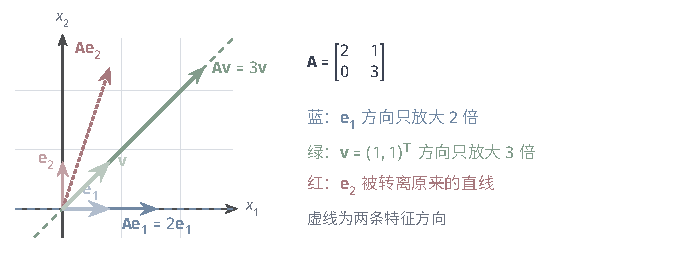
\includegraphics[width=112mm]{figures/01-mathematical-preliminaries-upper/03-linear-spaces/tikz/comprehension-additions/operator-eigenvectors.pdf}
  \caption{特征向量只被伸缩、不被转向。算子$T(x_1,x_2)=(2x_1+x_2,3x_2)$在标准基下的矩阵为$\bm A=\left[\begin{smallmatrix}2&1\\0&3\end{smallmatrix}\right]$，它把$\bm e_1$送到$2\bm e_1$，把$\bm v=(1,1)^{\top}$送到$3\bm v$，二者都留在各自的虚线上；$\bm e_2$被送到$(1,3)^{\top}$，偏离了原来的直线，所以不是特征向量。}
  \label{fig:ls-operator-eigenvectors}
\end{figure}

并非每个算子都有实特征向量。下面的反例中，每个非零向量都被转离原来的直线。
\begin{example}[反例：平面旋转没有实特征向量]
\label{ex:ls-rotation-no-real-eigenvector}
给定平面上逆时针旋转$90^\circ$的算子$R(x_1,x_2)=(-x_2,x_1)$。检验它是否有实特征值。设实数$\lambda$与向量$(x_1,x_2)$满足$R(x_1,x_2)=\lambda(x_1,x_2)$，即
\[
 -x_2=\lambda x_1,\qquad x_1=\lambda x_2 .
\]
把第二式代入第一式得$-x_2=\lambda^2x_2$，即$(1+\lambda^2)x_2=0$。由于$1+\lambda^2>0$，只能$x_2=0$，进而$x_1=\lambda x_2=0$。结论：对任何实数$\lambda$，满足等式的只有零向量，所以$R$没有实特征值，也没有实特征向量。
\end{example}

\subsection{特征空间与不变子空间}

同一个特征值往往不止对应一条特征方向。固定特征值$\lambda$，满足$T\bm v=\lambda\bm v$的全部向量连同零向量组成集合$\ker(T-\lambda\,\operatorname{id}_V)$，称为$\lambda$的\term{特征空间}（eigenspace）。它是一个线性映射的核，因而是子空间。例如$\bm I_2$的每个非零向量都是属于$1$的特征向量，特征空间是整个平面；而示例~\ref{ex:ls-operator-eigenvector-check}中属于$2$的特征空间只是$\bm e_1$所在的直线，因为$\bm A-2\bm I=\left[\begin{smallmatrix}0&1\\0&1\end{smallmatrix}\right]$的核由第二坐标为零的向量组成。

特征空间是一类更一般的子空间的特例。若子空间$S$满足$T(S)\subseteq S$，就称$S$为$T$的\term{不变子空间}（invariant subspace）。这时作用不会把$S$中的向量带出$S$，于是可以把$T$限制在$S$上单独研究。特征空间是不变子空间，因为其中的向量只被乘以$\lambda$，仍留在其中。

一维不变子空间恰好就是特征方向。若$\bm v\neq\bm0$且$\operatorname{span}\{\bm v\}$不变，则$T\bm v$落在这条直线上，是$\bm v$的倍数；反之，若$T\bm v=\lambda\bm v$，则$T(c\bm v)=\lambda c\bm v$仍在这条直线上。高于一维的不变子空间却未必含有特征方向：整个平面对$90^\circ$旋转不变，而示例~\ref{ex:ls-rotation-no-real-eigenvector}说明其中没有一条特征方向。第~\ref{sec:ls-general-square-spectrum}节将看到，这样的二维不变子空间对应一对共轭的复特征值。

\subsection{特征多项式}
\label{sec:ls-characteristic-polynomial}

示例~\ref{ex:ls-operator-eigenvector-check}中的特征向量是先猜出、再验证的。能否系统地求出全部特征值？对$n$阶方阵$\bm A$，$\lambda$是特征值，当且仅当齐次方程$(\bm A-\lambda\bm I)\bm v=\bm0$有非零解，即$\ker(\bm A-\lambda\bm I)\neq\{\bm0\}$。由第~\ref{sec:ls-injective-surjective-invertible}节的等价条件，这又等价于$\operatorname{rank}(\bm A-\lambda\bm I)<n$，也等价于$\bm A-\lambda\bm I$不可逆。

不可逆又等价于行列式为零，这一步用到第~\ref{sec:ls-determinant-properties}节的两条性质。若方阵$\bm M$可逆，乘法性给出$\det\bm M\det(\bm M^{-1})=\det\bm I=1$，故$\det\bm M\neq0$；反之若$\det\bm M\neq0$，古典伴随恒等式说明$\operatorname{adj}(\bm M)/\det\bm M$就是$\bm M$的逆。所以$\lambda$是$\bm A$的特征值，当且仅当$\det(\bm A-\lambda\bm I)=0$。第~\ref{sec:ls-similarity-properties}节把每个$\operatorname{rank}(\bm A-c\bm I)$都列为相似不变量；现在可以看出，使这个秩小于$n$的数$c$恰好就是特征值。

为了把这个条件写成首项系数为正的多项式，注意$\det(\lambda\bm I-\bm A)=(-1)^n\det(\bm A-\lambda\bm I)$，二者同时为零。定义
\begin{equation}
 p_{\bm A}(z)=\det(z\bm I-\bm A),
 \label{eq:matrix-analysis-characteristic-polynomial}
\end{equation}
称为\term{特征多项式}（characteristic polynomial），就得到：$\bm A$的实特征值恰为$p_{\bm A}$的实根。在行列式的排列展开中，对角线一项是$\prod_i(z-a_{i,i})$；其余每一项至少有两个因子取自非对角位置，含$z$的因子至多$n-2$个。所以只有对角线一项含$z^n$，$p_{\bm A}$是首项系数为$1$的$n$次实多项式，至多有$n$个不同的根。求出一个特征值$\lambda$以后，再解齐次方程$(\bm A-\lambda\bm I)\bm v=\bm0$，就得到它的特征空间。

用特征多项式可以重新求出前面两个例子的特征值，而不必猜测特征向量。
\begin{example}[用特征多项式求特征值]
\label{ex:ls-characteristic-polynomial-two-by-two}
给定示例~\ref{ex:ls-operator-eigenvector-check}的$\bm A=\left[\begin{smallmatrix}2&1\\0&3\end{smallmatrix}\right]$，以及示例~\ref{ex:ls-rotation-no-real-eigenvector}的旋转在标准基下的矩阵$\bm R=\left[\begin{smallmatrix}0&-1\\1&0\end{smallmatrix}\right]$。二者的特征多项式为
\[
 \begin{aligned}
 p_{\bm A}(z)&=\det\begin{bmatrix}z-2&-1\\0&z-3\end{bmatrix}=(z-2)(z-3),\\
 p_{\bm R}(z)&=\det\begin{bmatrix}z&1\\-1&z\end{bmatrix}=z^2+1 .
 \end{aligned}
\]
结论：$\bm A$的特征值为$2$与$3$，与示例~\ref{ex:ls-operator-eigenvector-check}验证的两条特征方向相符；$z^2+1$对任何实数$z$都为正，没有实根，所以$\bm R$没有实特征值，与示例~\ref{ex:ls-rotation-no-real-eigenvector}的直接验证一致。
\end{example}
$\bm A$的情形可以推广到任意三角矩阵：三角矩阵$\bm A$的$z\bm I-\bm A$仍是三角矩阵，行列式是对角元之积$\prod_i(z-a_{i,i})$，所以三角矩阵的特征值就是它的对角元。

特征多项式在每个特征值处取零。若把矩阵本身代入特征多项式，又会得到什么？这里的代入是指把多项式中的$z^j$换成$\bm A^j$，常数项$c_0$换成$c_0\bm I$。先看一个例子。
\begin{example}[把矩阵代入它的特征多项式]
\label{ex:ls-cayley-hamilton-two-by-two}
给定$\bm A=\left[\begin{smallmatrix}2&1\\0&3\end{smallmatrix}\right]$。由示例~\ref{ex:ls-characteristic-polynomial-two-by-two}，$p_{\bm A}(z)=(z-2)(z-3)=z^2-5z+6$。计算$p_{\bm A}(\bm A)=\bm A^2-5\bm A+6\bm I$：
\[
 \bm A^2=\begin{bmatrix}4&5\\0&9\end{bmatrix},\qquad
 \bm A^2-5\bm A+6\bm I
 =\begin{bmatrix}4-10+6&5-5+0\\0&9-15+6\end{bmatrix}
 =\bm0 .
\]
结论：把$\bm A$代入自身的特征多项式，得到零矩阵。
\end{example}
这不是巧合。证明的工具是第~\ref{sec:ls-determinant-properties}节的古典伴随恒等式（定理~\ref{thm:ls-adjugate-identity}）$\bm M\operatorname{adj}(\bm M)=\det(\bm M)\bm I$。令$\bm M=z\bm I-\bm A$，得
\[
 (z\bm I-\bm A)\operatorname{adj}(z\bm I-\bm A)=p_{\bm A}(z)\bm I .
\]
$\operatorname{adj}(z\bm I-\bm A)$的每个元素都是$z\bm I-\bm A$的一个带符号的$n-1$阶余子式，它是$z$的多项式，次数不超过$n-1$。按$z$的幂次整理，可以写成$\operatorname{adj}(z\bm I-\bm A)=\sum_{j=0}^{n-1}z^j\bm B_j$，其中$\bm B_j$是不含$z$的常数矩阵。
\begin{theorem}[Cayley--Hamilton定理]
\label{thm:ls-cayley-hamilton}
设$n$阶方阵$\bm A$的特征多项式为$p_{\bm A}(z)=z^n+c_{n-1}z^{n-1}+\cdots+c_0$，则
\[
 p_{\bm A}(\bm A)
 =\bm A^n+c_{n-1}\bm A^{n-1}+\cdots+c_1\bm A+c_0\bm I=\bm0.
\]
\end{theorem}
\begin{proof}
把$\operatorname{adj}(z\bm I-\bm A)=\sum_{j=0}^{n-1}z^j\bm B_j$代入上式，左边为$\sum_jz^{j+1}\bm B_j-\sum_jz^j\bm A\bm B_j$。两边每个元素都是$z$的多项式，且对所有实数$z$相等，所以同次项的系数相等。记$c_n=1$，比较$z$的各次幂系数：
\[
 \begin{aligned}
 &z^n: &&\bm B_{n-1}=\bm I;\\
 &z^j\ (1\leq j\leq n-1): &&\bm B_{j-1}-\bm A\bm B_j=c_j\bm I;\\
 &z^0: &&-\bm A\bm B_0=c_0\bm I .
 \end{aligned}
\]
把$z^j$项的等式左乘$\bm A^j$（$j=0,\ldots,n$）后相加。右边恰为$\sum_jc_j\bm A^j=p_{\bm A}(\bm A)$；左边为
\[
 \bm A^n\bm B_{n-1}+\sum_{j=1}^{n-1}\bigl(\bm A^j\bm B_{j-1}-\bm A^{j+1}\bm B_j\bigr)-\bm A\bm B_0 ,
\]
其中相邻项逐对相消，总和为零。
\end{proof}
证明只用到行列式与古典伴随，既不需要先求出特征值，也不要求$p_{\bm A}$有实根。

定理的一个直接推论是，高次幂可以由低次幂表示。由$p_{\bm A}(\bm A)=\bm0$得$\bm A^n=-\sum_{j=0}^{n-1}c_j\bm A^j$，即$\bm A^n$是$\bm I,\bm A,\ldots,\bm A^{n-1}$的线性组合。两边再左乘$\bm A$，右端出现的$\bm A^n$同样用这个式子代换，可知$\bm A^{n+1}$也是这些矩阵的线性组合；归纳可得，所有$\bm A^k$（$k\geq n$）都是。因此，对任意向量$\bm g$，$\bm A^k\bm g$（$k\geq n$）都是$\bm g,\bm A\bm g,\ldots,\bm A^{n-1}\bm g$的线性组合，序列$\bm g,\bm A\bm g,\bm A^2\bm g,\ldots$张成的子空间在前$n$项之后不再增大。第~\ref{chap:linear-equations-and-optimization}章判断Sylvester方程何时有唯一解时，要用到这个定理。

同一个特征值可以是特征多项式的重根。这时，关于这个特征值有两种“个数”需要区分。根$\lambda$在$p_{\bm A}$中的重数称为\term{代数重数}（algebraic multiplicity），特征空间的维数$\dim\ker(\bm A-\lambda\bm I)$称为\term{几何重数}（geometric multiplicity）。下面的例子说明二者可以不同。
\begin{example}[代数重数大于几何重数]
\label{ex:ls-multiplicity-gap}
给定
\[
 \bm J=\begin{bmatrix}0.8&1\\0&0.8\end{bmatrix}.
\]
它是上三角矩阵，特征多项式为$p_{\bm J}(z)=(z-0.8)^2$，所以唯一的特征值$0.8$的代数重数为$2$。再求特征空间：
\[
 \bm J-0.8\bm I=\begin{bmatrix}0&1\\0&0\end{bmatrix},\qquad
 (\bm J-0.8\bm I)\begin{bmatrix}x_1\\x_2\end{bmatrix}=\begin{bmatrix}x_2\\0\end{bmatrix},
\]
它为零当且仅当$x_2=0$，所以特征空间是$(1,0)^{\top}$所在的直线。结论：特征值$0.8$的代数重数为$2$，几何重数只有$1$。
\end{example}
两种重数的一般关系，以及它们怎样决定能否找到由特征向量组成的基，在第~\ref{sec:ls-matrix-powers}节讨论。对一般的算子$T$，可以取任一组基把它写成矩阵，再求特征多项式与两种重数；下一小节说明，这样得到的结果不依赖基的选取。

\subsection{相似不变性}
\label{sec:ls-eigen-similarity-invariance}

第~\ref{sec:ls-similarity-properties}节列出了相似保持的量：秩、零空间的维数、每个$\operatorname{rank}(\bm A-c\bm I)$，以及行列式与迹。特征值、特征多项式与两种重数是否也在其中？若是，它们就属于算子本身，可以用任意一组基下的矩阵计算。下面设$\bm B=\bm P^{-1}\bm A\bm P$，其中$\bm P$可逆。

先看特征值与几何重数。若$\bm A\bm v=\lambda\bm v$且$\bm v\neq\bm0$，则
\[
 \bm B(\bm P^{-1}\bm v)=\bm P^{-1}\bm A\bm P\bm P^{-1}\bm v=\bm P^{-1}\bm A\bm v=\lambda\bm P^{-1}\bm v .
\]
$\bm P$可逆保证$\bm P^{-1}\bm v\neq\bm0$，所以$\lambda$也是$\bm B$的特征值，相应的特征向量是$\bm P^{-1}\bm v$；交换$\bm A,\bm B$的角色即得反向结论。同样的计算说明$\ker(\bm B-\lambda\bm I)=\bm P^{-1}\ker(\bm A-\lambda\bm I)$，而可逆矩阵把子空间映成同维数的子空间，所以每个特征值的几何重数不变。这一结论也可以由式~\eqref{eq:ls-similarity-shifted-rank}取$c=\lambda$、再用秩零度定理换成核的维数得到。

更进一步，整个特征多项式不变：
\[
 p_{\bm B}(z)=\det(z\bm I-\bm P^{-1}\bm A\bm P)=\det\bigl(\bm P^{-1}(z\bm I-\bm A)\bm P\bigr)=p_{\bm A}(z),
\]
中间一步用了$z\bm I=\bm P^{-1}(z\bm I)\bm P$，最后一步用了第~\ref{sec:ls-similarity-properties}节的恒等式$\det(\bm P^{-1}\bm M\bm P)=\det\bm M$。所以算子的特征多项式可以用任意一组基下的矩阵计算，代数重数也是相似不变量。

特征多项式的系数还说明了行列式与迹为什么是相似不变量：它们就是$p_{\bm A}$的两个系数，至多差一个符号。令$z=0$，得常数项$p_{\bm A}(0)=\det(-\bm A)=(-1)^n\det\bm A$。再看$z^{n-1}$的系数。上一小节已经指出，排列展开中除对角线一项外，每一项含$z$的因子至多$n-2$个；所以$z^{n-1}$只来自$\prod_i(z-a_{i,i})$，系数为$-\sum_ia_{i,i}=-\operatorname{tr}\bm A$。于是
\[
 p_{\bm A}(z)=z^n-(\operatorname{tr}\bm A)\,z^{n-1}+\cdots+(-1)^n\det\bm A .
\]

若$p_{\bm A}$能分解为实一次因子之积$\prod_{i=1}^n(z-\lambda_i)$，其中每个特征值按代数重数重复列出，把右端展开后比较$z^{n-1}$的系数与常数项，得
\[
 \operatorname{tr}\bm A=\sum_{i=1}^n\lambda_i,\qquad \det\bm A=\prod_{i=1}^n\lambda_i .
\]
例如示例~\ref{ex:ls-operator-eigenvector-check}的$\bm A$有$\operatorname{tr}\bm A=5=2+3$，$\det\bm A=6=2\cdot3$。第~\ref{sec:ls-general-square-spectrum}节把特征多项式的复根也算作特征值以后，这两个等式对每个方阵都成立。

相似不变量只能用来否定相似：某个相似不变量不同，两个矩阵就不相似；不变量全部相同，两个矩阵却未必相似。第~\ref{sec:ls-similarity-conditions}节比较过$\bm I_2$与$\left[\begin{smallmatrix}1&1\\0&1\end{smallmatrix}\right]$，现在可以用特征值的语言重新说明二者为什么不相似。
\begin{example}[反例：特征多项式相同而不相似]
\label{ex:ls-same-charpoly-not-similar}
给定$\bm I_2$与
\[
 \bm J_1=\begin{bmatrix}1&1\\0&1\end{bmatrix}.
\]
二者都是上三角矩阵，对角元都是$1$，所以$p_{\bm I_2}(z)=p_{\bm J_1}(z)=(z-1)^2$，特征值$1$的代数重数都是$2$。另一方面，
\[
 \bm I_2-\bm I_2=\bm0,\qquad
 \bm J_1-\bm I_2=\begin{bmatrix}0&1\\0&0\end{bmatrix},
\]
前者的核是整个平面，后者的核只是$(1,0)^{\top}$所在的直线，几何重数分别为$2$与$1$。结论：二者的特征多项式相同，但几何重数不同；由于几何重数是相似不变量，它们不相似。
\end{example}
所以特征多项式相同只是相似的必要条件。比较各特征值的几何重数是更细的必要条件，但一般仍不足以判定相似；完整的相似分类需要Jordan标准形，本书不展开。下一节只处理最重要、也最常用的一类矩阵：与对角矩阵相似的矩阵。

\subsection{不同特征值的特征向量}
\label{sec:ls-eigenvector-independence}

特征方向能否多到组成一组基？先要说明，属于不同特征值的特征向量不会彼此重复，即它们线性无关。设$\bm v_1,\ldots,\bm v_r$分别属于互不相同的特征值$\lambda_1,\ldots,\lambda_r$，假设它们线性相关。在所有非平凡的线性依赖中取项数最少的一个，重新编号后记为$\sum_{j=1}^s c_j\bm v_j=\bm0$，其中各$c_j\neq0$；单个特征向量非零，不能单独构成依赖，所以$s\geq2$。两边作用$T-\lambda_1\operatorname{id}_V$：第一项变为零，其余各项变为$c_j(\lambda_j-\lambda_1)\bm v_j$。特征值互不相同，这些系数仍非零，于是得到一个只有$s-1$项的非平凡依赖，与$s$最少矛盾。所以$\bm v_1,\ldots,\bm v_r$线性无关。由于$n$维空间中线性无关的向量至多$n$个，$n$维空间上的算子至多有$n$个不同特征值，这与特征多项式的次数给出的上界一致。

由此，不同特征值的特征空间之和是直和。设$\sum_\lambda\bm w_\lambda=\bm0$，每个$\bm w_\lambda$属于相应的特征空间；其中非零的$\bm w_\lambda$是属于不同特征值的特征向量，它们线性无关，所以只能每个$\bm w_\lambda=\bm0$。把各特征空间的基合在一起，它们的任一线性组合都可以按特征值分组写成$\sum_\lambda\bm w_\lambda$；若组合为零，则每个$\bm w_\lambda=\bm0$，而每组基本身线性无关，所以全部系数为零。因此各特征空间的基合在一起仍线性无关。例如示例~\ref{ex:ls-operator-eigenvector-check}中的$\bm e_1$与$(1,1)^{\top}$属于不同的特征值$2$与$3$，不必另行验证，它们自动线性无关，在平面上组成一组基。

至此，本节开头的四个问题都有了回答。被算子只伸缩的方向是特征方向，伸缩倍数是特征值；特征值是特征多项式的实根，求出特征值后解齐次方程即得特征空间。特征值、特征多项式和两种重数都不随基改变，属于算子本身。属于不同特征值的特征向量线性无关，所以$n$维空间上的算子至多有$n$个不同特征值。途中还得到了Cayley--Hamilton定理：$\bm A$的高次幂都能用$\bm I,\bm A,\ldots,\bm A^{n-1}$表示。剩下的问题是特征向量什么时候多到足以组成一组基，这是下一节的对角化问题。

% 第6章第2节：基于可逆矩阵的对角化（特征基下的矩阵与幂、可对角化的定义与判据及不能对角化的情形、步骤与算例）。

\section{基于可逆矩阵的对角化}
\label{sec:ls-matrix-powers}
\label{sec:ch06-powers-spectrum}

上一节找到了被算子只伸缩的方向，并证明属于不同特征值的特征向量线性无关。本节回答由此引出的问题：有了由特征向量组成的基，算子的矩阵变成什么样，又能怎样利用？这样的基什么时候存在？换到这组基所用的换基矩阵只要求可逆，不要求各列互相垂直，所以本节的对角化是用一般的可逆矩阵作相似变换。

\subsection{特征基下的矩阵}
\label{sec:matrix-analysis-spectrum}

设$\bm v_1,\ldots,\bm v_n$是由算子$T$的特征向量组成的基，$T\bm v_j=\lambda_j\bm v_j$。按第~\ref{sec:ls-map-representation}节的约定，$T$在这组基下的矩阵的第$j$列是$T\bm v_j=\lambda_j\bm v_j$的坐标，即第$j$个位置为$\lambda_j$、其余位置为零。所以这个矩阵在主对角线以外全为零，每个基方向被独立地伸缩。示例~\ref{ex:ls-operator-eigenvector-check}中的$(\bm e_1,(1,1)^{\top})$就是这样一组基。换到这组基，正是第~\ref{sec:ls-similarity}节的相似变换$\bm P^{-1}\bm A\bm P=\operatorname{diag}(2,3)$；在图~\ref{fig:ls-similarity-change-of-basis-flow}中，基向量围成的平行四边形只沿两条特征方向分别伸长$2$倍和$3$倍。

这一观察也可以写成矩阵等式。设$\bm A$是$T$在标准基下的矩阵，把特征向量的标准坐标排成$\bm V=[\bm v_1,\ldots,\bm v_n]$。$\bm V$的各列是新基向量的旧坐标，所以它正是第~\ref{sec:ls-similarity}节的换基矩阵；各列线性无关，所以$\bm V$可逆（第~\ref{sec:ls-injective-surjective-invertible}节）。按乘积的列读法，$\bm A\bm V$的第$j$列是$\bm A\bm v_j=\lambda_j\bm v_j$；右乘对角矩阵$\bm\Lambda=\operatorname{diag}(\lambda_1,\ldots,\lambda_n)$把第$j$列乘以$\lambda_j$，所以$\bm V\bm\Lambda$的第$j$列也是$\lambda_j\bm v_j$。于是$\bm A\bm V=\bm V\bm\Lambda$，两边左乘或右乘$\bm V^{-1}$，即得
\[
 \bm V^{-1}\bm A\bm V=\bm\Lambda,\qquad \bm A=\bm V\bm\Lambda\bm V^{-1}.
\]

对角形式的好处在反复作用时最明显。同一个方阵反复作用，是矩阵乘法最常见的用法之一：定常迭代$\bm x^{(k+1)}=\bm A\bm x^{(k)}$走$k$步后得到$\bm x^{(k)}=\bm A^k\bm x^{(0)}$。第~\ref{sec:ls-matrix-power-rules}节规定了矩阵幂的写法，但直接连乘会不断混合各个坐标，看不出$\bm A^k$在$k$很大时是什么样子。把$\bm A=\bm V\bm\Lambda\bm V^{-1}$连乘$k$次，相邻的$\bm V^{-1}\bm V$相消（这就是式~\eqref{eq:ls-similarity-product}后面的$\bm B^k=\bm P^{-1}\bm A^k\bm P$），得到
\begin{equation}
 \bm A^k=\bm V\bm\Lambda^k\bm V^{-1},\qquad
 \bm\Lambda^k=\operatorname{diag}(\lambda_1^k,\ldots,\lambda_n^k).
 \label{eq:ls-diagonalization-power}
\end{equation}
于是求幂只需对对角元逐个乘方。三个因子可以从右向左读：$\bm V^{-1}\bm x^{(0)}$给出初值在各特征方向上的坐标，$\bm\Lambda^k$把第$j$个坐标乘以$\lambda_j^k$，$\bm V$再把结果合回标准坐标。上一节已经看到，沿特征方向有$\bm A^k\bm v=\lambda^k\bm v$；式~\eqref{eq:ls-diagonalization-power}把这一点推广到任意初值。

下面用一个上三角矩阵演示这种计算：先把一个初值拆成特征方向上的分量，再对所有初值一并写出矩阵幂。
\begin{example}[用特征向量计算矩阵幂]
\label{ex:ls-triangular-power}
给定
\[
 \bm A=\begin{bmatrix}0.8&4\\0&0.5\end{bmatrix},
\]
计算$\bm A^k$。

第一步，求特征值与特征向量。$\bm A$是上三角矩阵，特征值为对角元$0.8$与$0.5$。直接验证
\[
 \bm A\begin{bmatrix}1\\0\end{bmatrix}=0.8\begin{bmatrix}1\\0\end{bmatrix},\qquad
 \bm A\begin{bmatrix}-40/3\\1\end{bmatrix}
 =\begin{bmatrix}-32/3+4\\0.5\end{bmatrix}
 =0.5\begin{bmatrix}-40/3\\1\end{bmatrix},
\]
所以$\bm v_1=(1,0)^{\top}$与$\bm v_2=(-40/3,1)^{\top}$是特征向量。

第二步，计算一条轨迹。初值$(0,1)^{\top}$不在特征方向上，先把它拆成$(0,1)^{\top}=\tfrac{40}{3}\bm v_1+\bm v_2$。两个分量每作用一次分别乘以$0.8$与$0.5$，由线性性，
\[
 \bm A^k\begin{bmatrix}0\\1\end{bmatrix}
 =\frac{40}{3}\,0.8^k\bm v_1+0.5^k\bm v_2
 =\begin{bmatrix}\tfrac{40}{3}(0.8^k-0.5^k)\\0.5^k\end{bmatrix}.
\]
$k=1$时得$(4,0.5)^{\top}$，与直接计算$\bm A(0,1)^{\top}$一致。

第三步，对所有初值一并计算，即应用式~\eqref{eq:ls-diagonalization-power}。取$\bm V=\left[\begin{smallmatrix}1&-40/3\\0&1\end{smallmatrix}\right]$，则$\bm V^{-1}=\left[\begin{smallmatrix}1&40/3\\0&1\end{smallmatrix}\right]$，
\[
 \bm A^k=\bm V\begin{bmatrix}0.8^k&0\\0&0.5^k\end{bmatrix}\bm V^{-1}
 =\begin{bmatrix}0.8^k&\tfrac{40}{3}(0.8^k-0.5^k)\\0&0.5^k\end{bmatrix}.
\]
结论：$\bm A^k$的第二列正是第二步的轨迹；整个迭代拆成两个独立的数列，分别按$0.8^k$与$0.5^k$衰减。
\end{example}
这种计算依赖一个前提：特征向量足以组成整个空间的一组基。下一小节讨论这个前提何时成立。

\subsection{可对角化的定义与判据}

\paragraph{定义与特征向量判据}
上一小节说明，有了由特征向量组成的基，$\bm A$就相似于一个对角矩阵。把相似于对角矩阵这一性质取作定义。
\begin{definition}[实可对角化]
\label{def:ls-real-diagonalizable}
设$\bm A$是$n$阶实方阵。若存在$n$阶实可逆矩阵$\bm V$与实对角矩阵$\bm\Lambda$使$\bm V^{-1}\bm A\bm V=\bm\Lambda$，即$\bm A$相似于实对角矩阵，就称$\bm A$\term{实可对角化}（diagonalizable over the reals）；求出这样的$\bm V$与$\bm\Lambda$，称为把$\bm A$对角化。
\end{definition}
“实”表示$\bm V$与$\bm\Lambda$的元素都是实数。本书在实数范围内讨论，下文所说的可对角化都指实可对角化。

哪些矩阵可以对角化？下面的判据把问题化为特征向量够不够多。
\begin{theorem}[对角化判据]
\label{thm:ls-diagonalization-criterion}
$n$阶实方阵$\bm A$实可对角化，当且仅当$\bm A$有$n$个线性无关的实特征向量。这时以这些特征向量为列组成$\bm V$，以相应特征值按同一顺序组成$\bm\Lambda=\operatorname{diag}(\lambda_1,\ldots,\lambda_n)$，就有$\bm V^{-1}\bm A\bm V=\bm\Lambda$。
\end{theorem}
\begin{proof}
设$\bm V$的各列为$\bm v_1,\ldots,\bm v_n$，$\bm\Lambda=\operatorname{diag}(\lambda_1,\ldots,\lambda_n)$。上一小节的列读法对任意这样的$\bm V$与$\bm\Lambda$都成立，它给出
\[
 \bm A\bm V=\bm V\bm\Lambda
 \quad\Longleftrightarrow\quad
 \bm A\bm v_j=\lambda_j\bm v_j,\qquad j=1,\ldots,n.
\]
若$\bm A$有$n$个线性无关的特征向量，以它们为列的$\bm V$可逆，左乘$\bm V^{-1}$即得$\bm V^{-1}\bm A\bm V=\bm\Lambda$。反过来，若$\bm V^{-1}\bm A\bm V=\bm\Lambda$，左乘$\bm V$得$\bm A\bm V=\bm V\bm\Lambda$，于是每列都满足$\bm A\bm v_j=\lambda_j\bm v_j$；$\bm V$可逆，所以各列线性无关，从而都非零，它们是$n$个线性无关的特征向量。
\end{proof}
由第~\ref{sec:ls-eigenvector-independence}节，属于不同特征值的特征向量线性无关，由此得到一个常用的充分条件：$n$阶实方阵若有$n$个互不相同的实特征值，就实可对角化。示例~\ref{ex:ls-triangular-power}的矩阵即属此类。这个条件不是必要的：单位矩阵$\bm I_n$只有一个特征值$1$，本身却已经是对角矩阵。

\paragraph{不能对角化的矩阵}
判据要求$n$个线性无关的实特征向量，这一要求可能在两处得不到满足。其一，实特征值不够。示例~\ref{ex:ls-rotation-no-real-eigenvector}与示例~\ref{ex:ls-characteristic-polynomial-two-by-two}已经说明，平面上的$90^\circ$旋转$\bm R=\left[\begin{smallmatrix}0&-1\\1&0\end{smallmatrix}\right]$没有实特征值，也就没有实特征向量，所以不能实对角化。其二，实特征值有了，特征向量却不够。示例~\ref{ex:ls-multiplicity-gap}中的$\bm J=\left[\begin{smallmatrix}0.8&1\\0&0.8\end{smallmatrix}\right]$只有特征值$0.8$，而特征向量只有$(1,0)^{\top}$的倍数，凑不出两个线性无关的特征向量，所以$\bm J$也不能对角化。

对这样的矩阵，式~\eqref{eq:ls-diagonalization-power}不再可用，幂也不再是纯粹的乘方。下面直接计算$\bm J^k$。
\begin{example}[不能对角化矩阵的幂]
\label{ex:ls-jordan-block-power}
给定$\bm J=\left[\begin{smallmatrix}0.8&1\\0&0.8\end{smallmatrix}\right]$，计算$\bm J^k$。把$\bm J$写成$0.8\bm I+\bm N$，其中
\[
 \bm N=\begin{bmatrix}0&1\\0&0\end{bmatrix},\qquad \bm N^2=\bm0 .
\]
$0.8\bm I$与$\bm N$可交换，所以二项式展开成立；又因为$j\geq2$时$\bm N^j=\bm0$，展开后只剩前两项：
\[
 \bm J^k=(0.8\bm I+\bm N)^k=0.8^k\bm I+k\,0.8^{k-1}\bm N=\begin{bmatrix}0.8^k&k\,0.8^{k-1}\\0&0.8^k\end{bmatrix}.
\]
右上角相邻两项之比为$\dfrac{(k+1)\,0.8^{k}}{k\,0.8^{k-1}}=0.8\cdot\dfrac{k+1}{k}$，它在$k<4$时大于$1$，在$k>4$时小于$1$。结论：右上角的$k\,0.8^{k-1}$随$k$先增大、后衰减，不能由单个特征值的乘方描述。
\end{example}

\paragraph{重数判据}
两个反例分别缺了什么？$\bm R$的特征多项式$z^2+1$不能分解为实一次因子；$\bm J$的特征多项式$(z-0.8)^2$分解了，但特征值$0.8$的几何重数$1$小于代数重数$2$。下面说明，这两种缺陷恰好是全部障碍。于是能否对角化可以直接由特征多项式和特征空间的维数判断，而不必逐个尝试特征向量。

先证明几何重数不超过代数重数。设特征值$\lambda$的特征空间维数为$g$，取它的一组基，并扩充成全空间的一组基。在新基下，前$g$个基向量都被送到自身的$\lambda$倍，所以$\bm A$相似于分块上三角矩阵$\left[\begin{smallmatrix}\lambda\bm I_g&*\\\bm0&\bm C\end{smallmatrix}\right]$。相似不改变特征多项式（第~\ref{sec:ls-eigen-similarity-invariance}节），所以可以用这个分块矩阵计算$p_{\bm A}$。用$z\bm I$减去它以后，前$g$列都只在对角位置上有非零元素$z-\lambda$。沿第一列按余子式展开（第~\ref{sec:ls-determinant-properties}节），得到$z-\lambda$乘以一个形状相同、但只剩$g-1$个这种列的行列式；重复$g$次，即得$p_{\bm A}(z)=(z-\lambda)^g\,p_{\bm C}(z)$。所以代数重数至少为$g$。示例~\ref{ex:ls-multiplicity-gap}说明不等号可以严格成立。

由此得到可以计算的判据：$\bm A$实可对角化，当且仅当$p_{\bm A}$能分解为实一次因子之积，且每个特征值的几何重数等于代数重数。

先证充分性。$p_{\bm A}$分解为$n$个实一次因子时，各特征值的代数重数之和为$n$；几何重数与代数重数逐个相等，所以几何重数之和也是$n$。由第~\ref{sec:ls-eigenvector-independence}节，不同特征值的特征空间之和是直和，各特征空间的基合在一起仍线性无关，于是恰好得到$n$个线性无关的特征向量；由对角化判据，$\bm A$可对角化。

再证必要性。若$\bm A=\bm V\bm\Lambda\bm V^{-1}$，则由相似不变性，$p_{\bm A}=p_{\bm\Lambda}=\prod_i(z-\lambda_i)$已分解为实一次因子。对每个特征值$\lambda$，它在$\bm\Lambda$对角线上出现的次数既是代数重数，也是$\bm\Lambda-\lambda\bm I$的零空间维数，即$\bm\Lambda$的几何重数。由第~\ref{sec:ls-eigen-similarity-invariance}节，相似不改变几何重数，所以$\bm A$的两种重数也相等。

有$n$个互不相同的实特征值时，每个代数重数都是$1$，几何重数至少为$1$又不超过$1$，判据的条件自动满足，这就回到了前面的充分条件。

\subsection{对角化的步骤与算例}

按判据，对角化分四步。第一步，求出特征多项式$p_{\bm A}$的全部实根，即全部实特征值。第二步，对每个特征值$\lambda$解齐次方程$(\bm A-\lambda\bm I)\bm v=\bm0$，得到特征空间的一组基。第三步，若这些向量合起来共有$n$个，就以它们为列组成$\bm V$，以对应的特征值按同一顺序组成$\bm\Lambda$。第四步，核对$\bm A\bm V=\bm V\bm\Lambda$。若特征多项式不能分解为实一次因子，或某个特征空间的维数小于相应的代数重数，过程就在第一步或第三步停止，矩阵不能实对角化，这正是上一小节的两种情形。

下面用一个两状态转移的例子走一遍这四步。设一个群体在两个状态之间转移：每期处于状态一的个体有$10\%$转入状态二，处于状态二的个体有$20\%$转入状态一。记第$k$期两个状态所占的比例为$\bm x^{(k)}=(x_1^{(k)},x_2^{(k)})^{\top}$，则下一期状态一的比例为$0.9x_1^{(k)}+0.2x_2^{(k)}$，状态二的比例为$0.1x_1^{(k)}+0.8x_2^{(k)}$，即
\[
 \bm x^{(k+1)}=\bm A\bm x^{(k)},\qquad
 \bm A=\begin{bmatrix}0.9&0.2\\0.1&0.8\end{bmatrix}.
\]
\begin{example}[两状态转移矩阵的对角化]
\label{ex:ls-transition-matrix-diagonalization}
给定转移矩阵$\bm A=\left[\begin{smallmatrix}0.9&0.2\\0.1&0.8\end{smallmatrix}\right]$，按四步把它对角化。

第一步，求特征值：
\[
 p_{\bm A}(z)=(z-0.9)(z-0.8)-0.2\cdot0.1=z^2-1.7z+0.7=(z-1)(z-0.7),
\]
得$\lambda_1=1$、$\lambda_2=0.7$。两个特征值不同，所以$\bm A$可对角化。

第二步，求特征空间。$\lambda_1=1$时$\bm A-\bm I=\left[\begin{smallmatrix}-0.1&0.2\\0.1&-0.2\end{smallmatrix}\right]$，两行成比例，方程化为$-0.1x_1+0.2x_2=0$，取$\bm v_1=(2,1)^{\top}$。$\lambda_2=0.7$时$\bm A-0.7\bm I=\left[\begin{smallmatrix}0.2&0.2\\0.1&0.1\end{smallmatrix}\right]$，方程化为$x_1+x_2=0$，取$\bm v_2=(1,-1)^{\top}$。

第三步，组成
\[
 \bm V=\begin{bmatrix}2&1\\1&-1\end{bmatrix},\qquad
 \bm\Lambda=\begin{bmatrix}1&0\\0&0.7\end{bmatrix},\qquad
 \bm V^{-1}=\frac13\begin{bmatrix}1&1\\1&-2\end{bmatrix},
\]
其中$\bm V^{-1}$由二阶逆矩阵公式得到，$\det\bm V=-3$。

第四步，核对：
\[
 \bm A\bm v_1=\begin{bmatrix}1.8+0.2\\0.2+0.8\end{bmatrix}=\bm v_1,\qquad
 \bm A\bm v_2=\begin{bmatrix}0.9-0.2\\0.1-0.8\end{bmatrix}=0.7\bm v_2,
\]
所以$\bm A\bm V=\bm V\bm\Lambda$。也可以用上一节的系数关系作快速检查：$\operatorname{tr}\bm A=1.7=1+0.7$，$\det\bm A=0.7=1\cdot0.7$。

结论：$\bm A=\bm V\bm\Lambda\bm V^{-1}$，$\bm V$的两列分别是属于特征值$1$与$0.7$的特征向量。
\end{example}

有了这个分解，就可以按式~\eqref{eq:ls-diagonalization-power}回答这个群体的长期去向。
\begin{example}[转移矩阵的长期比例]
\label{ex:ls-transition-matrix-long-run}
沿用示例~\ref{ex:ls-transition-matrix-diagonalization}的分解，计算$\bm A^k$以及$k\to\infty$时两个状态的比例。由式~\eqref{eq:ls-diagonalization-power}，
\[
 \bm A^k=\bm V\begin{bmatrix}1&0\\0&0.7^k\end{bmatrix}\bm V^{-1}
 =\frac13\begin{bmatrix}2+0.7^k&2-2\cdot0.7^k\\1-0.7^k&1+2\cdot0.7^k\end{bmatrix};
\]
$k=1$时右端正是$\bm A$。若开始时全部个体处于状态一，即$\bm x^{(0)}=(1,0)^{\top}$，则$\bm x^{(k)}$是$\bm A^k$的第一列：
\[
 \bm x^{(k)}=\frac13\begin{bmatrix}2+0.7^k\\1-0.7^k\end{bmatrix}
 \to\begin{bmatrix}2/3\\1/3\end{bmatrix}\qquad(k\to\infty).
\]
对一般的初始比例$\bm x^{(0)}=(a,1-a)^{\top}$，$\bm V^{-1}\bm x^{(0)}$给出它在两条特征方向上的分量：
\[
 \bm V^{-1}\bm x^{(0)}=\frac13\begin{bmatrix}a+(1-a)\\a-2(1-a)\end{bmatrix}=\begin{bmatrix}1/3\\(3a-2)/3\end{bmatrix}.
\]
沿$\bm v_1$的分量总是$1/3$，沿$\bm v_2$的分量每期乘以$0.7$而趋于零。结论：无论从什么比例出发，长期比例都是$\tfrac13\bm v_1=(2/3,1/3)^{\top}$。
\end{example}

至此，本节开头的问题有了回答。在由特征向量组成的基下，算子的矩阵是对角的；以特征向量为列的$\bm V$把$\bm A$化为$\bm\Lambda$，反复作用化为特征值的乘方，$\bm A^k=\bm V\bm\Lambda^k\bm V^{-1}$。$n$阶矩阵可对角化，当且仅当它有$n$个线性无关的实特征向量；等价地，特征多项式分解为实一次因子，且每个特征值的几何重数等于代数重数。实特征值不足或特征向量不足时，矩阵不能对角化；后一种情形的幂含有随$k$增长的多项式因子。

对角化回答了“能否找到只被伸缩的基方向”，却没有要求这些方向互相垂直。示例~\ref{ex:ls-transition-matrix-diagonalization}中的两条特征方向$(2,1)^{\top}$与$(1,-1)^{\top}$内积为$1$，并不垂直。换到这样的基，求新坐标要解方程，新坐标的平方和也不等于原向量长度的平方。下一节追问，哪些矩阵能用正交矩阵对角化，即具有一组标准正交的特征向量。至于不能对角化的矩阵在标准正交基下能化到多简单，以及特征向量接近线性相关时矩阵幂有多大，分别留给第~\ref{sec:ls-general-square-spectrum}节与第~\ref{sec:ls-matrix-power-behavior}节。

% 第6章第3节：基于正交矩阵的对角化（谱定理、Rayleigh商与谱的极值性质、对称矩阵的函数）。

\section{基于正交矩阵的对角化}
\label{sec:ls-spectral-theory}

上一节用可逆矩阵$\bm V$对角化，只要求基由特征向量组成，没有要求这些方向互相垂直。本节追问：哪些矩阵能用正交矩阵对角化，即找到一组标准正交的特征向量？答案是实对称矩阵，这一结论称为谱定理。有了这种分解，特征值还获得第二种含义：它们是二次型在单位球面上的极值，因此可以不求特征向量而比较、估计特征值。沿互相垂直的特征方向，还可以定义矩阵的平方根、对数等函数。

\subsection{谱定理}
\label{sec:ls-symmetric-spectral-decomposition}

先说明为什么希望特征方向互相垂直。若$\bm q_1,\ldots,\bm q_d$是$\mathbb R^d$的标准正交基，把它们排成正交矩阵$\bm Q$，则$\bm Q^{-1}=\bm Q^\top$。于是换基不必解方程：向量$\bm x$的新坐标就是内积$c_i=\bm q_i^\top\bm x$，长度也保持不变，$\lVert\bm x\rVert_2^2=\sum_ic_i^2$（第~\ref{sec:ls-orthonormal-bases}节）。所以，若方阵$\bm A$能写成$\bm A=\bm Q\bm\Lambda\bm Q^\top$，其中$\bm\Lambda$为实对角矩阵，它的作用就最容易看清：先用内积读出各方向的坐标，再把第$i$个坐标乘以$\lambda_i$，最后合回去。

哪些矩阵能这样写？必要条件很容易看出：若$\bm A=\bm Q\bm\Lambda\bm Q^\top$，则$\bm A^\top=\bm Q\bm\Lambda^\top\bm Q^\top=\bm A$，所以$\bm A$必须对称。对称矩阵也就是第~\ref{sec:ls-adjoints}节的自伴算子在标准坐标下的矩阵。本小节证明这一条件也是充分的。

下面把对称矩阵记为$\bm S$。证明的思路是：在单位球面上最大化二次型$\bm x^\top\bm S\bm x$，说明取到最大值的方向是一个特征方向，再在与它垂直的子空间中重复这一步。为此先要确认最大值确实能取到。

二次型在单位球面上有界：单位向量的每个坐标满足$|x_i|\leq1$，所以$|\bm x^\top\bm S\bm x|\leq\sum_{i,j}|s_{i,j}||x_i||x_j|\leq\sum_{i,j}|s_{i,j}|$。由确界原理，它有上确界$M$。取单位向量序列$\bm x_k$使$\bm x_k^\top\bm S\bm x_k\to M$，记$\bm x_k$的第$i$个坐标为$x_{k,i}$，各坐标数列都在$[-1,1]$中。由有界数列必有收敛子列（定理~\ref{thm:analysis-bounded-subsequence}），先取子列使第一个坐标收敛，再在这个子列中取子列使第二个坐标收敛，如此进行$d$次，得到一个每个坐标都收敛的子列，记其极限为$\bm x_*$。沿这个子列取极限，由极限的四则运算得$\lVert\bm x_*\rVert_2^2=\lim\sum_ix_{k,i}^2=1$与$\bm x_*^\top\bm S\bm x_*=\lim\bm x_k^\top\bm S\bm x_k=M$。所以$M$在单位球面上的点$\bm x_*$处取到，是最大值。

从这个最大点出发，逐个找出互相正交的特征方向，就得到下面的结论，称为\term{谱定理}（spectral theorem）。

\begin{theorem}[谱定理]
\label{thm:ls-real-symmetric-spectral}
\label{thm:matrix-analysis-symmetric-spectral-theorem}
\label{sec:ch06-triangular-spectrum}
设$\bm S\in\mathbb R^{d\times d}$满足$\bm S=\bm S^\top$，则存在正交矩阵$\bm Q=[\bm q_1,\ldots,\bm q_d]$与实对角矩阵$\bm\Lambda=\operatorname{diag}(\lambda_1,\dots,\lambda_d)$，使
\begin{equation}
 \bm S=\bm Q\bm\Lambda\bm Q^\top,
 \qquad \bm S\bm q_i=\lambda_i\bm q_i.
 \label{eq:matrix-analysis-symmetric-eigendecomposition}
\end{equation}
对任意$\bm x=\sum_i c_i\bm q_i$，二次型展开为
\begin{equation}
 \bm x^\top\bm S\bm x=\sum_{i=1}^d\lambda_i c_i^2.
 \label{eq:matrix-analysis-quadratic-spectral-form}
\end{equation}
\end{theorem}

\begin{proof}
分三步。

第一步，找出最大方向。由定理前的论证，二次型$q(\bm x)=\bm x^\top\bm S\bm x$在单位球面上取到最大值，记最大值为$\lambda_1$、最大点为$\bm q_1$。对任意$\bm x\neq\bm0$，$\bm x/\lVert\bm x\rVert_2$在单位球面上，而$q$是二次齐次的，所以
\[
 q(\bm x)=\lVert\bm x\rVert_2^2\,q\bigl(\bm x/\lVert\bm x\rVert_2\bigr)\leq\lambda_1\lVert\bm x\rVert_2^2 .
\]

第二步，说明$\bm q_1$是特征向量。任取与$\bm q_1$正交的$\bm h$和实数$t$，把$\bm x=\bm q_1+t\bm h$代入上面的不等式。由勾股定理$\lVert\bm q_1+t\bm h\rVert_2^2=1+t^2\lVert\bm h\rVert_2^2$；又由$\bm S$对称，$\bm q_1^\top\bm S\bm h=\bm h^\top\bm S\bm q_1$，于是
\[
 \lambda_1+2t\,\bm h^\top\bm S\bm q_1+t^2\bm h^\top\bm S\bm h
 \leq\lambda_1+t^2\lambda_1\lVert\bm h\rVert_2^2 ,
\]
即$2t\,\bm h^\top\bm S\bm q_1\leq t^2c$，其中$c=\lambda_1\lVert\bm h\rVert_2^2-\bm h^\top\bm S\bm h$。取$t>0$，两边除以$t$得$2\bm h^\top\bm S\bm q_1\leq tc$，令$t\to0^+$得$\bm h^\top\bm S\bm q_1\leq0$；取$t<0$，除以$t$时不等号反向，令$t\to0^-$得$\bm h^\top\bm S\bm q_1\geq0$。所以$\bm h^\top\bm S\bm q_1=0$。这对所有$\bm h\perp\bm q_1$成立，说明$\bm S\bm q_1$在$\bm q_1$的正交补中没有分量，只能是$\bm q_1$的倍数：$\bm S\bm q_1=(\bm q_1^\top\bm S\bm q_1)\bm q_1=\lambda_1\bm q_1$。

第三步，对正交补归纳。对$\bm h\perp\bm q_1$，$\bm q_1^\top(\bm S\bm h)=(\bm S\bm q_1)^\top\bm h=\lambda_1\bm q_1^\top\bm h=0$，所以$\bm S$把$d-1$维子空间$\bm q_1^\perp$映到自身；对其中任意$\bm u,\bm v$仍有$\bm u^\top\bm S\bm v=\bm v^\top\bm S\bm u$，在$\bm q_1^\perp$的标准正交基下，$\bm S$的作用由一个$d-1$阶对称矩阵表示。对它重复前两步，得到$\bm q_2\perp\bm q_1$与$\lambda_2$；逐次降维到一维，就得到标准正交的$\bm q_1,\dots,\bm q_d$与实数$\lambda_1,\ldots,\lambda_d$。

最后，把$\bm x=\sum_ic_i\bm q_i$代入二次型：交叉项$c_ic_j\bm q_i^\top\bm S\bm q_j=c_ic_j\lambda_j\bm q_i^\top\bm q_j$在$i\neq j$时为零，只剩$\sum_i\lambda_ic_i^2$。
\end{proof}

证明只用到单位球面上的极值与对称性，没有借助复数或特征多项式。按构造，后一步是在更小的子空间上求最大值，最大值不会超过上一步，所以$\lambda_1\geq\lambda_2\geq\cdots\geq\lambda_d$。把$\bm Q\bm\Lambda\bm Q^\top$按列展开，谱分解也可写成秩一矩阵之和
\[
 \bm S=\sum_{i=1}^d\lambda_i\bm q_i\bm q_i^\top ,
\]
其中$\bm q_i\bm q_i^\top$是到$\bm q_i$方向的正交投影。下面用一个二阶矩阵看这种分解。
\begin{example}[二阶对称矩阵的谱分解]
\label{ex:ls-symmetric-spectral-two-by-two}
给定
\[
 \bm S=\begin{bmatrix}2&1\\1&2\end{bmatrix},
\]
求它的谱分解。特征多项式为$p_{\bm S}(z)=(z-2)^2-1=(z-3)(z-1)$，特征值为$3$与$1$。直接验证$\bm S(1,1)^\top=3(1,1)^\top$、$\bm S(1,-1)^\top=(1,-1)^\top$，单位化得$\bm q_1=(1,1)^\top/\sqrt2$、$\bm q_2=(1,-1)^\top/\sqrt2$。两个投影矩阵为
\[
 \bm q_1\bm q_1^\top=\frac12\begin{bmatrix}1&1\\1&1\end{bmatrix},\qquad
 \bm q_2\bm q_2^\top=\frac12\begin{bmatrix}1&-1\\-1&1\end{bmatrix},
\]
于是
\[
 3\bm q_1\bm q_1^\top+\bm q_2\bm q_2^\top
 =\frac12\begin{bmatrix}3+1&3-1\\3-1&3+1\end{bmatrix}=\bm S .
\]
结论：$\bm S=3\bm q_1\bm q_1^\top+\bm q_2\bm q_2^\top$，即$\bm S$把$(1,1)^\top$方向放大$3$倍，保持$(1,-1)^\top$方向不变。
\end{example}

二次型展开式~\eqref{eq:matrix-analysis-quadratic-spectral-form}还直接给出定号性的判据。$\bm x^\top\bm S\bm x=\sum_i\lambda_ic_i^2$对所有$\bm x$非负，当且仅当每个$\lambda_i\geq0$；必要性只需取$\bm x=\bm q_i$。所以$\bm S\succeq0$当且仅当全部特征值非负；同理，$\bm S\succ0$当且仅当全部特征值为正。

特征值有重复时，$\bm Q$不唯一：对应特征空间内的任意一组标准正交基都可以作为这部分的$\bm q_i$。但每个特征空间$\ker(\bm S-\lambda\bm I)$本身由$\bm S$唯一确定。

\subsection{Rayleigh商与谱的极值性质}
\label{sec:ls-rayleigh-extremal}
\label{sec:ls-sphere-existence}
\label{sec:linear-algebra-constrained-estimation}
\label{sec:ls-sphere-solve}

谱定理的证明中，最大特征值$\lambda_1$就是单位球面上二次型的最大值。其余特征值是否也有类似的极值含义？若有，就可以不求特征向量而直接比较、估计特征值：比较两个矩阵的特征值，只需比较它们的二次型。本小节给出这种刻画，并用它解决几类带尺度约束的优化问题。

\paragraph{Rayleigh商}

二次型$\bm x^\top\bm S\bm x$随$\bm x$的长度按平方增长，直接比较不同方向会被长度主导。把长度除掉，就得到只依赖方向的量，称为\term{Rayleigh商}（Rayleigh quotient）。
\begin{definition}[Rayleigh商]
\label{def:matrix-analysis-rayleigh-quotient}
对实对称矩阵$\bm S$与$\bm x\neq\bm0$，
\begin{equation}
 R_{\bm S}(\bm x)=\frac{\bm x^\top\bm S\bm x}{\bm x^\top\bm x}.
 \label{eq:matrix-analysis-rayleigh-quotient}
\end{equation}
\end{definition}
把$\bm x$换成$c\bm x$（$c\neq0$）时分子分母同乘$c^2$，Rayleigh商不变，因此求它的极值等价于在单位球面上求二次型的极值。对单位向量$\bm x=\sum_ic_i\bm q_i$，有$\sum_ic_i^2=1$，由二次型展开式，
\[
 R_{\bm S}(\bm x)=\sum_{i=1}^d\lambda_ic_i^2 ,
\]
它是各特征值以$c_i^2$为权的加权平均。图~\ref{fig:ls-sphere-constrained-extremum}用一个二阶对称矩阵画出这一关系：二次型的水平椭圆在特征方向处与单位圆相切，切点处取到极值。

\begin{figure}[htbp]
  \centering
  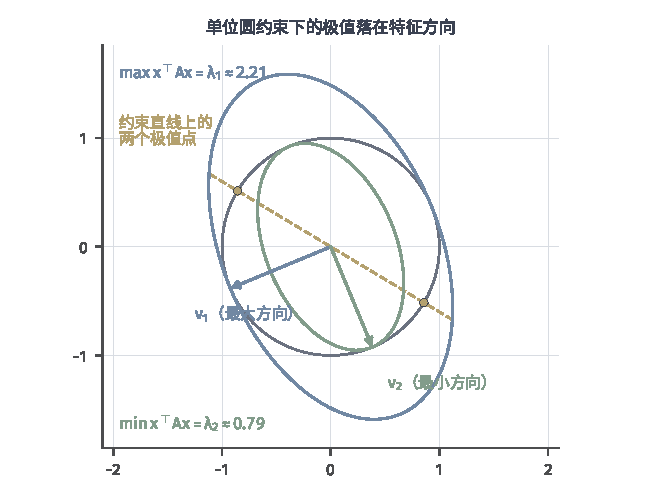
\includegraphics[width=112mm]{figures/01-mathematical-preliminaries-upper/03-linear-spaces/matplotlib/ls-sphere-constrained-extremum/ls-sphere-constrained-extremum.pdf}
  \caption{单位圆约束下的极值落在特征方向。$\bm S=\left[\begin{smallmatrix}2&0.5\\0.5&1\end{smallmatrix}\right]$，
  灰圆为$\lVert\bm x\rVert=1$。蓝椭圆$\bm x^\top\bm S\bm x=\lambda_1\approx2.21$在
  $\pm\bm v_1$处与单位圆相切（最大值），绿椭圆$=\lambda_2\approx0.79$在$\pm\bm v_2$处
  相切（最小值）；黄色虚线为子空间约束直线，其上黄点是该约束下的两个极值。
  $\lambda_{1,2}=(3\pm\sqrt2)/2$。固定复算。}
  \label{fig:ls-sphere-constrained-extremum}
\end{figure}

加权平均介于被平均各数的最小值与最大值之间，由此立即得到两端特征值的极值刻画。
\begin{theorem}[Rayleigh--Ritz]
\label{thm:matrix-analysis-rayleigh-ritz}
\label{eq:matrix-analysis-rayleigh-ritz}
设$\bm S$的特征值为$\lambda_1\geq\cdots\geq\lambda_d$，对应标准正交特征向量$\bm q_1,\ldots,\bm q_d$，则
\begin{equation*}
 \max_{\bm x\neq\bm0}R_{\bm S}(\bm x)=\lambda_1,\qquad
 \min_{\bm x\neq\bm0}R_{\bm S}(\bm x)=\lambda_d,
\end{equation*}
分别在$\bm q_1$与$\bm q_d$取到。
\end{theorem}
\begin{proof}
权重$c_i^2$非负且总和为$1$，所以$\lambda_d\leq\sum_i\lambda_ic_i^2\leq\lambda_1$；取$\bm x=\bm q_1$时只有$c_1=1$，得$\lambda_1$，取$\bm x=\bm q_d$时得$\lambda_d$。
\end{proof}
极值本身唯一，取到极值的方向却未必唯一：$\lambda_1$重复时，其特征空间中每个单位向量都给出最大值；只有在目标特征值单重时，最优方向才唯一（差一个符号）。

\paragraph{齐次最小二乘}
\label{sec:linear-algebra-homogeneous-estimation}

Rayleigh--Ritz定理的一个直接应用是带尺度约束的拟合。有时模型写成$\bm A\bm h\approx\bm0$，只关心$\bm h$各分量之间的比例。这时直接最小化$\lVert\bm A\bm h\rVert_2^2$总会得到平凡解$\bm h=\bm0$，必须先固定尺度。固定$\lVert\bm h\rVert_2=1$后得到的问题称为\term{齐次最小二乘}（homogeneous least squares）：
\begin{equation}
 \min_{\lVert\bm h\rVert_2=1}\ \lVert\bm A\bm h\rVert_2^2
 =\min_{\lVert\bm h\rVert_2=1}\bm h^\top\bm A^\top\bm A\bm h.
 \label{eq:linear-algebra-homogeneous-least-squares}
\end{equation}
右端是对称矩阵$\bm A^\top\bm A$的二次型在单位球面上的最小值。由Rayleigh--Ritz定理，最小值是$\bm A^\top\bm A$的最小特征值，最优$\bm h$是对应的单位特征向量。若$\bm A$有非零零空间，最小值为零，任一单位零空间向量都是最优解。下面的例子属于这种情形。
\begin{example}[一个方程的齐次最小二乘]
\label{ex:ls-homogeneous-least-squares-one-row}
给定一行矩阵$\bm A=[\,1\ -2\,]$。

按式~\eqref{eq:linear-algebra-homogeneous-least-squares}，最优解是$\bm A^\top\bm A$最小特征值的单位特征向量。计算得
\[
 \begin{aligned}
 \bm A^\top\bm A&=\begin{bmatrix}1&-2\\-2&4\end{bmatrix},\\
 \bm A^\top\bm A\,(2,1)^\top&=\bm0,\qquad
 \bm A^\top\bm A\,(1,-2)^\top=5\,(1,-2)^\top .
 \end{aligned}
\]
所以$\bm A^\top\bm A$的特征值为$0$与$5$。

最小特征值$0$对应的单位特征向量为$\bm h=\pm(2,1)^\top/\sqrt5$，它满足$\bm A\bm h=h_1-2h_2=0$。

结论：最小值为$0$，最优解为$\bm h=\pm(2,1)^\top/\sqrt5$；两个符号给出同一个比例$h_1:h_2=2:1$。
\end{example}

\paragraph{Courant--Fischer最小最大原理}

Rayleigh--Ritz定理只刻画两端的特征值。中间的$\lambda_k$不再是整个空间上的极值，但可以借助子空间刻画：在$k$维子空间上取Rayleigh商的最小值，再让子空间变动，取这些最小值中的最大者。

\begin{theorem}[Courant--Fischer]
\label{thm:matrix-analysis-courant-fischer}
\label{eq:matrix-analysis-courant-fischer}
对$k=1,\ldots,d$，
\begin{equation*}
 \lambda_k=\max_{\dim\mathcal V=k}\ \min_{\bm x\in\mathcal V,\bm x\neq\bm0}R_{\bm S}(\bm x)
 =\min_{\dim\mathcal W=d-k+1}\ \max_{\bm x\in\mathcal W,\bm x\neq\bm0}R_{\bm S}(\bm x).
\end{equation*}
\end{theorem}
\begin{proof}
先证第一式。取$\mathcal V_k=\operatorname{span}\{\bm q_1,\dots,\bm q_k\}$，其中单位向量的Rayleigh商是$\lambda_1,\ldots,\lambda_k$的加权平均，不小于$\lambda_k$，所以左端的最大值至少为$\lambda_k$。反过来，任取$k$维子空间$\mathcal V$，令$\mathcal W_k=\operatorname{span}\{\bm q_k,\dots,\bm q_d\}$，它是$d-k+1$维的。由维数公式，
\[
 \dim(\mathcal V\cap\mathcal W_k)\geq\dim\mathcal V+\dim\mathcal W_k-d=1,
\]
所以$\mathcal V$中有非零向量$\bm x$落在$\mathcal W_k$里。它的Rayleigh商是$\lambda_k,\ldots,\lambda_d$的加权平均，不大于$\lambda_k$，因此$\mathcal V$上Rayleigh商的最小值不超过$\lambda_k$。两方面合起来即得第一式。

第二式交换两组特征向量的角色：$\mathcal W_k$上Rayleigh商的最大值恰为$\lambda_k$；任意$d-k+1$维子空间都与$\mathcal V_k$有非零公共向量，其Rayleigh商不小于$\lambda_k$。
\end{proof}
定理只涉及子空间与Rayleigh商，不要求先知道特征向量；第~\ref{sec:ls-spectral-value-sensitivity}节正是用它比较扰动前后的特征值。同样的加权平均论证还可以一次处理$k$个方向，得到前$k$个与后$k$个特征值之和的极值刻画。

\begin{theorem}[迹极值]
\label{thm:matrix-analysis-trace-minimum}
对列标准正交的$\bm V\in\mathbb R^{d\times k}$，
\begin{equation}
 \sum_{i=d-k+1}^{d}\lambda_i\leq\operatorname{tr}(\bm V^\top\bm S\bm V)\leq\sum_{i=1}^{k}\lambda_i,
 \label{eq:matrix-analysis-trace-minimum}
\end{equation}
上下界分别由前$k$个与后$k$个特征向量张成的子空间取到。
\end{theorem}
\begin{proof}
代入$\bm S=\sum_i\lambda_i\bm q_i\bm q_i^\top$，得$\operatorname{tr}(\bm V^\top\bm S\bm V)=\sum_i\lambda_iw_i$，其中$w_i=\lVert\bm V^\top\bm q_i\rVert_2^2$。由$\bm V^\top\bm V=\bm I$得$\lVert\bm V^\top\rVert_2=1$，所以$0\leq w_i\leq1$；又$\sum_iw_i=\lVert\bm V^\top\bm Q\rVert_{\mathrm F}^2=\lVert\bm V\rVert_{\mathrm F}^2=k$。在这两个约束下，
\[
 \begin{aligned}
 \sum_i\lambda_iw_i-\sum_{i\leq k}\lambda_i
 &=\sum_{i\leq k}\lambda_i(w_i-1)+\sum_{i>k}\lambda_iw_i\\
 &\leq\lambda_k\sum_{i\leq k}(w_i-1)+\lambda_k\sum_{i>k}w_i
 =\lambda_k\Bigl(\sum_iw_i-k\Bigr)=0,
 \end{aligned}
\]
其中不等号用到$w_i-1\leq0$、$\lambda_i\geq\lambda_k$（$i\leq k$）与$w_i\geq0$、$\lambda_i\leq\lambda_k$（$i>k$）。这就是上界；对$-\bm S$应用上界即得下界。$\bm V$取前$k$个或后$k$个特征向量时，等号成立。
\end{proof}
上界说明，用$k$维子空间保留二次型的“能量”，最好的选择是前$k$个特征方向，这是主成分分析的代数基础。

\paragraph{广义特征问题}

有时长度不按欧氏范数度量，而按第~\ref{sec:ls-weighted-inner-products}节的加权内积度量，约束$\lVert\bm x\rVert_2=1$相应地换成$\bm x^\top\bm B\bm x=1$（$\bm B\succ0$），要比较的是广义Rayleigh商$\bm x^\top\bm S\bm x/\bm x^\top\bm B\bm x$。它可以化回普通情形。由定理~\ref{thm:ls-gram-factor}写$\bm B=\bm L^\top\bm L$，$\bm L$可逆，令$\bm z=\bm L\bm x$，则$\bm x^\top\bm B\bm x=\bm z^\top\bm z$，而
\[
 \frac{\bm x^\top\bm S\bm x}{\bm x^\top\bm B\bm x}
 =\frac{\bm z^\top\bm L^{-\top}\bm S\bm L^{-1}\bm z}{\bm z^\top\bm z}
\]
是对称矩阵$\bm L^{-\top}\bm S\bm L^{-1}$的普通Rayleigh商。其特征方程$\bm L^{-\top}\bm S\bm L^{-1}\bm z=\mu\bm z$左乘$\bm L^\top$并换回$\bm v=\bm L^{-1}\bm z$，就是下面的方程。
\begin{definition}[广义特征值]
\label{def:matrix-analysis-generalized-eigenvalue}
对实对称$\bm S$与$\bm B\succ0$，称满足
\begin{equation}
 \bm S\bm v=\mu\bm B\bm v,\qquad\bm v\neq\bm0
 \label{eq:matrix-analysis-generalized-eigenproblem}
\end{equation}
的$\mu$为广义特征值，$\bm v$为广义特征向量，求解它们的问题称为\term{广义特征问题}（generalized eigenvalue problem）。
\end{definition}
对$\bm L^{-\top}\bm S\bm L^{-1}$应用谱定理可知：广义特征值全为实数；广义特征向量可以取为$\bm B$正交的，即$\bm v_i^\top\bm B\bm v_j=\delta_{i,j}$（因为$\bm z_i=\bm L\bm v_i$标准正交）；最大、最小广义特征值就是广义Rayleigh商的最大、最小值。

计算时也应走这条换元的路。直接对$\bm B^{-1}\bm S$求特征值虽然得到同样的$\mu$，但$\bm B^{-1}\bm S$一般不对称，会丢掉对称结构带来的正交性与数值稳定性。

\subsection{对称矩阵的函数}
\label{sec:ls-matrix-functions}
\label{sec:matrix-analysis-functions-structured-operations}

多项式$p(\bm S)$可以直接用矩阵的幂与加法算出。平方根、对数、指数这类非多项式函数怎样作用于矩阵？谱定理提示了做法。由$\bm S=\bm Q\bm\Lambda\bm Q^\top$与$\bm Q^\top\bm Q=\bm I$，连乘时相邻的$\bm Q^\top\bm Q$相消，得$\bm S^k=\bm Q\bm\Lambda^k\bm Q^\top$；再按系数相加，得$p(\bm S)=\bm Q\,p(\bm\Lambda)\,\bm Q^\top$。也就是说，多项式在每个特征方向上只作用于对应的特征值。把这一观察作为定义，推广到一般函数。

\paragraph{沿特征方向的定义}

设$\bm S=\bm Q\bm\Lambda\bm Q^\top$，$f$是定义在全部特征值$\lambda_i$上的实函数，令
\begin{equation}
 f(\bm S)=\bm Q\operatorname{diag}\bigl(f(\lambda_1),\ldots,f(\lambda_d)\bigr)\bm Q^\top.
 \label{eq:ls-symmetric-spectral-function}
\end{equation}
$\bm Q$不唯一，需要检查结果是否依赖它的选取。把同一特征值$\lambda$的特征向量归为一组，$\sum_{\lambda_i=\lambda}\bm q_i\bm q_i^\top$是到特征空间$\ker(\bm S-\lambda\bm I)$的正交投影$\bm P_\lambda$，它只依赖这个子空间，与子空间内基的选取无关。于是$f(\bm S)=\sum_\lambda f(\lambda)\bm P_\lambda$，求和遍历不同的特征值，结果由$\bm S$唯一确定。$f(z)=z^k$时，定义回到矩阵幂$\bm S^k$，与已有运算相容。

矩阵函数作用在特征方向上，而不是逐元素作用。下面的例子对照这两种做法。
\begin{example}[矩阵平方根与逐元素开方]
\label{ex:ls-matrix-square-root-two-by-two}
给定示例~\ref{ex:ls-symmetric-spectral-two-by-two}的$\bm S=3\bm q_1\bm q_1^\top+\bm q_2\bm q_2^\top$，取$f(z)=\sqrt z$。按式~\eqref{eq:ls-symmetric-spectral-function}，
\[
 f(\bm S)=\sqrt3\,\bm q_1\bm q_1^\top+\bm q_2\bm q_2^\top
 =\frac12\begin{bmatrix}\sqrt3+1&\sqrt3-1\\\sqrt3-1&\sqrt3+1\end{bmatrix}.
\]
它的平方为
\[
 \frac14\begin{bmatrix}(\sqrt3+1)^2+(\sqrt3-1)^2&2(\sqrt3+1)(\sqrt3-1)\\2(\sqrt3+1)(\sqrt3-1)&(\sqrt3+1)^2+(\sqrt3-1)^2\end{bmatrix}
 =\frac14\begin{bmatrix}8&4\\4&8\end{bmatrix}=\bm S .
\]
逐元素开方得到$\left[\begin{smallmatrix}\sqrt2&1\\1&\sqrt2\end{smallmatrix}\right]$，它的平方是$\left[\begin{smallmatrix}3&2\sqrt2\\2\sqrt2&3\end{smallmatrix}\right]\neq\bm S$。结论：沿特征方向定义的$f(\bm S)$满足$f(\bm S)^2=\bm S$，逐元素开方的结果则不满足。
\end{example}

\paragraph{平方根、实幂与对数}

$\bm S$半正定时，全部$\lambda_i\geq0$，可取$f(z)=\sqrt z$，得到\term{矩阵平方根}（matrix square root）
\[
 \bm S^{1/2}=\bm Q\operatorname{diag}(\sqrt{\lambda_1},\ldots,\sqrt{\lambda_d})\bm Q^\top ,
\]
它半正定且$(\bm S^{1/2})^2=\bm S$。

方程$\bm X^2=\bm S$一般有多个解，例如$\bm I$与$-\bm I$的平方都是$\bm I$；但要求$\bm X$半正定后，解是唯一的。设半正定的$\bm X=\sum_j\mu_j\bm p_j\bm p_j^\top$（$\mu_j\geq0$，$\bm p_j$标准正交）满足$\bm X^2=\bm S$，则$\bm S=\sum_j\mu_j^2\bm p_j\bm p_j^\top$，即每个$\bm p_j$都是$\bm S$的特征向量，特征值为$\mu_j^2$。于是$\bm S$的$\lambda$特征空间恰由满足$\mu_j^2=\lambda$的那些$\bm p_j$张成，而$\mu_j\geq0$迫使这些$\mu_j=\sqrt\lambda$。所以$\bm X$在$\bm S$的每个特征空间上都乘以$\sqrt\lambda$，这正是$\bm S^{1/2}$的作用，$\bm X=\bm S^{1/2}$。

$\bm S$正定时，全部$\lambda_i>0$，还可以取任意实幂$\bm S^\alpha$，例如$\alpha=-1/2$给出逆平方根；也可以取\term{矩阵对数}（matrix logarithm）$\log\bm S=\bm Q\operatorname{diag}(\log\lambda_1,\ldots,\log\lambda_d)\bm Q^\top$。有零特征值时，负幂与对数都没有定义。注意$\log\bm S$是矩阵，而$\log\det\bm S=\sum_i\log\lambda_i=\operatorname{tr}(\log\bm S)$是标量，二者不能混淆。

按定义计算需要完整的谱分解，代价较高。若只需计算$\lVert\bm S^{1/2}\bm x\rVert_2$或作用$\bm S^{-1/2}$做白化，可以用定理~\ref{thm:ls-gram-factor}的因子代替平方根：写$\bm S=\bm L^\top\bm L$，则$\lVert\bm L\bm x\rVert_2^2=\bm x^\top\bm S\bm x=\lVert\bm S^{1/2}\bm x\rVert_2^2$，两者给出同样的长度。第~\ref{chap:linear-equations-and-optimization}章的Cholesky分解把$\bm L$取成三角矩阵，那时作用$\bm L^{-1}$只需解三角方程。

至此，本节的问题有了回答。能用正交矩阵对角化的实矩阵，即具有一组标准正交特征向量的实矩阵，恰好是对称矩阵；谱分解$\bm S=\bm Q\bm\Lambda\bm Q^\top$把它写成沿互相垂直方向的伸缩。特征值同时是Rayleigh商的极值与最小最大值，可以只凭二次型来比较；矩阵函数沿特征方向逐个作用于特征值。但许多重要的方阵并不对称，例如平面旋转与示例~\ref{ex:ls-triangular-power}的上三角矩阵$\left[\begin{smallmatrix}0.8&4\\0&0.5\end{smallmatrix}\right]$。下一节讨论，对一般方阵，坚持用正交矩阵换基时最多能化到多简单。

% 第6章第4节：一般方阵的对角化（复特征值与谱半径、实Schur形与正规矩阵）。

\section{一般方阵的对角化}
\label{sec:ls-general-square-spectrum}

前两节的对角化各有前提：用可逆矩阵对角化，要求有足够多的实特征向量；用正交矩阵对角化，要求矩阵对称。不对称的方阵会在两处偏离这些前提。其一，实特征值可能不够：平面上的$90^\circ$旋转没有实特征向量，第~\ref{sec:ls-matrix-powers}节的对角化在第一步就停止。其二，即使可以对角化，特征向量也可能互不正交：示例~\ref{ex:ls-triangular-power}中矩阵的两条特征方向$(1,0)^\top$与$(-40/3,1)^\top$夹角只有约$4.3^\circ$（计算见示例~\ref{ex:ls-nonnormal-norm-radius}）。本节回答三个问题：非实的特征值在实空间中对应什么作用，怎样用一个数概括矩阵每作用一次的伸缩倍数；若坚持用正交矩阵换基，一般方阵最多能化到多接近对角的形式；什么样的方阵在这种换基下仍能化为分块对角形。

\subsection{复特征值与谱半径}

第~\ref{sec:ls-characteristic-polynomial}节的特征多项式$p_{\bm A}$是$d$次实系数多项式。由代数基本定理，它在复数范围内恰有$d$个根（计重数）。把这些根都称为$\bm A$的特征值，全体特征值组成的集合称为$\bm A$的\term{谱}（spectrum）。由于系数都是实数，若$p_{\bm A}(\lambda)=0$，两边取共轭即得$p_{\bm A}(\bar\lambda)=0$，所以非实根成共轭对出现。实特征值的情形与第~\ref{sec:ls-linear-operators}节相同。

第~\ref{sec:ls-eigen-similarity-invariance}节由系数比较得到$\operatorname{tr}\bm A=\sum_i\lambda_i$与$\det\bm A=\prod_i\lambda_i$，那里要求$p_{\bm A}$能分解为实一次因子。计入复特征值以后，$p_{\bm A}$在复数范围内总能分解为一次因子之积，同样的系数比较说明，这两个等式对每个方阵都成立。

非实特征值在实空间里对应什么作用？设$\lambda=a+\mathrm ib$（$b\neq0$）是特征值。复矩阵$\bm A-\lambda\bm I$的行列式为零，所以有非零的复向量$\bm u+\mathrm i\bm w$满足$\bm A(\bm u+\mathrm i\bm w)=(a+\mathrm ib)(\bm u+\mathrm i\bm w)$，其中$\bm u,\bm w$为实向量。比较两边的实部与虚部，得
\[
 \bm A\bm u=a\bm u-b\bm w,\qquad \bm A\bm w=b\bm u+a\bm w .
\]

这两个等式说明$\operatorname{span}\{\bm u,\bm w\}$在$\bm A$下不变。它是二维的，即$\bm u,\bm w$线性无关。否则$\bm u,\bm w$（不全为零）只张成一条直线$\operatorname{span}\{\bm y\}$，这条直线在$\bm A$下不变，所以$\bm A\bm y=\mu\bm y$，$\mu$为实数；而$\bm u+\mathrm i\bm w$是$\bm y$的复数倍，于是$\bm A(\bm u+\mathrm i\bm w)=\mu(\bm u+\mathrm i\bm w)$，得$\lambda=\mu$为实数，与$b\neq0$矛盾。所以$\operatorname{span}\{\bm u,\bm w\}$是二维实不变子空间。在基$(\bm u,\bm w)$下，$\bm A$的作用由矩阵
\[
 \begin{bmatrix}a&b\\-b&a\end{bmatrix}
 =|\lambda|\begin{bmatrix}\cos\phi&\sin\phi\\-\sin\phi&\cos\phi\end{bmatrix},
 \qquad \cos\phi=\frac{a}{|\lambda|},\ \sin\phi=\frac{b}{|\lambda|}
\]
表示，即$|\lambda|$倍的伸缩加一次旋转。

所以无论特征值是实是复，它的模长$|\lambda|$都是沿相应方向或平面每作用一次的伸缩倍数；复特征值的情形在基$(\bm u,\bm w)$的坐标中度量。全部特征值模长的最大值
\[
 \rho(\bm A)=\max_i|\lambda_i(\bm A)|
\]
称为\term{谱半径}（spectral radius）。例如$90^\circ$旋转的特征值为$\pm\mathrm i$，谱半径为$1$：它不改变长度，只改变方向。

\subsection{实Schur形与正规矩阵}

\paragraph{实Schur形}

一般方阵未必能对角化，更未必能用正交矩阵对角化。退一步，能否用正交矩阵把它化为上三角形？上三角形同样便于计算：对角元就是特征值，解方程和求幂都可以从最后一个坐标逐个向前推。实特征值不够时，实上三角形不可能存在，因为它的对角元就是特征值，必须全是实数；但允许对角线上出现$2\times2$块以后，答案总是肯定的。

\begin{theorem}[实Schur形]
\label{thm:ls-real-schur}
对任意$\bm A\in\mathbb R^{d\times d}$，存在正交矩阵$\bm Q$与分块上三角矩阵$\bm T$，使
\begin{equation}
 \bm A=\bm Q\bm T\bm Q^{\top},
 \label{eq:matrix-analysis-schur-decomposition}
\end{equation}
$\bm T$的对角块为$1\times1$（实特征值）或$2\times2$（一对共轭特征值），对角块下方全为零。$\bm A$的特征值就是各对角块的特征值。
\end{theorem}
\begin{proof}
对$d$归纳，思路与谱定理相同：先找一个不变子空间，再对其正交补降维。若$\bm A$有实特征值$\lambda$，取单位特征向量$\bm q_1$并扩充为正交矩阵$\bm Q_1=[\bm q_1,\bm Q_2]$。由$\bm A\bm q_1=\lambda\bm q_1$与$\bm Q_2^\top\bm q_1=\bm0$，$\bm Q_1^\top\bm A\bm Q_1$的第一列为$\lambda\bm e_1$，即
\[
 \bm Q_1^\top\bm A\bm Q_1=\begin{bmatrix}\lambda&*\\\bm0&\bm Q_2^\top\bm A\bm Q_2\end{bmatrix}.
\]
若没有实特征值，取上一小节得到的二维不变子空间，用它的一组标准正交基$\bm q_1,\bm q_2$同样扩充，得到左上角为$2\times2$块、其下方为零的分块形式，该块的特征值是$\lambda,\bar\lambda$。分块上三角矩阵的特征多项式是对角块特征多项式之积，所以右下块的特征值恰为其余特征值。对右下块应用归纳假设，再把两次正交变换合并，即得结论。
\end{proof}
实际计算先用Householder反射化为上Hessenberg形，再作带位移的QR迭代，标准数值软件都提供这一分解；本卷只使用它的存在性。第~\ref{sec:ls-sylvester-schur}节求解Sylvester方程时，用的正是这一形式。

\paragraph{正规矩阵}

Schur形什么时候是分块对角的？实对称矩阵是一例。这时$\bm T=\bm Q^\top\bm A\bm Q$仍对称，它的$2\times2$对角块也对称，特征值为实数，不可能对应一对共轭特征值，所以$\bm T$只有$1\times1$对角块，是上三角矩阵；对称的上三角矩阵只能是对角矩阵，这又一次得到谱定理。更一般地，第~\ref{sec:ls-adjoints}节把满足$TT^\star=T^\star T$的算子称为正规算子。在标准坐标下伴随就是转置，满足$\bm A^\top\bm A=\bm A\bm A^\top$的矩阵称为\term{正规矩阵}（normal matrix）；对称、反对称与正交矩阵都是正规的。

正规矩阵的Schur形$\bm T$分块对角。首先$\bm T$也正规：$\bm T^\top\bm T=\bm Q^\top\bm A^\top\bm A\bm Q=\bm Q^\top\bm A\bm A^\top\bm Q=\bm T\bm T^\top$。比较$\bm T^\top\bm T$与$\bm T\bm T^\top$的左上角对角块：前者是$\bm T_{1,1}^\top\bm T_{1,1}$，因为$\bm T$的第一块列只有$\bm T_{1,1}$非零；后者是$\sum_j\bm T_{1,j}\bm T_{1,j}^\top$。两边取迹，得
\[
 \lVert\bm T_{1,1}\rVert_{\mathrm F}^2=\lVert\bm T_{1,1}\rVert_{\mathrm F}^2+\sum_{j>1}\lVert\bm T_{1,j}\rVert_{\mathrm F}^2 ,
\]
故第一块行的非对角块全为零。去掉第一块后，剩下的矩阵仍正规，逐块推下去可知$\bm T$分块对角。

每个$2\times2$对角块$\left[\begin{smallmatrix}p&q\\r&s\end{smallmatrix}\right]$也正规。比较两边的$(1,1)$元得$q^2=r^2$。若$q=r$，块对称，特征值为实数，与$2\times2$块对应一对共轭特征值矛盾；所以$r=-q\neq0$。再比较$(1,2)$元得$2q(s-p)=0$，即$s=p$。于是每块都形如$\left[\begin{smallmatrix}a&b\\-b&a\end{smallmatrix}\right]$，是模长乘旋转。反过来，若正交矩阵$\bm Q$把$\bm A$化为分块对角矩阵$\bm T$，且每块是一个数或这种模长乘旋转的块，则每块与自己的转置可交换，$\bm T^\top\bm T=\bm T\bm T^\top$，从而$\bm A=\bm Q\bm T\bm Q^\top$正规。所以正规矩阵恰好是能用标准正交基化为这种分块对角形的实方阵。

总之，正规矩阵沿一组标准正交的方向或平面只作伸缩，或伸缩加旋转。$\bm T^k$仍分块对角，每块是$\lambda^k$或$|\lambda|^k$乘一个旋转，二范数为$|\lambda|^k$；正交变换又不改变谱范数，所以$\lVert\bm A^k\rVert_2=\lVert\bm T^k\rVert_2=\max_i|\lambda_i|^k=\rho(\bm A)^k$。也就是说，正规矩阵每一步的最大放大倍数恰好就是谱半径。

\paragraph{非正规矩阵}
由上一段，非正规矩阵的Schur形$\bm T$不可能是由数与模长乘旋转块组成的分块对角形：它要么含非零的非对角块，要么某个$2\times2$对角块本身不正规。非正规矩阵也不能用一组标准正交的特征向量对角化，否则它对称。这时矩阵范数可以远大于谱半径，下面的例子显示了这种分离。
\begin{example}[非正规矩阵的范数与谱半径]
\label{ex:ls-nonnormal-norm-radius}
给定示例~\ref{ex:ls-triangular-power}的$\bm A=\left[\begin{smallmatrix}0.8&4\\0&0.5\end{smallmatrix}\right]$，比较它的谱半径、一步的放大倍数与特征方向的夹角。

它不正规：$\bm A^\top\bm A$的$(1,1)$元为$0.8^2=0.64$，$\bm A\bm A^\top$的$(1,1)$元为$0.8^2+4^2=16.64$。特征值为$0.8$与$0.5$，所以$\rho(\bm A)=0.8$。一步作用把$(0,1)^\top$送到$(4,0.5)^\top$，长度为$\sqrt{16.25}>4$，所以$\lVert\bm A\rVert_2>4$。两条特征方向$\bm v_1=(1,0)^\top$与$\bm v_2=(-40/3,1)^\top$的夹角$\theta$满足
\[
 \cos\theta=\frac{|\bm v_1^\top\bm v_2|}{\lVert\bm v_1\rVert_2\lVert\bm v_2\rVert_2}
 =\frac{40/3}{\sqrt{(40/3)^2+1}}\approx0.997,
\]
即$\theta\approx4.3^\circ$。结论：两条特征方向几乎平行，一步的最大放大倍数超过$4$，而谱半径只有$0.8$。
\end{example}
谱半径描述反复作用的长期倍率，范数描述一步的最大放大；非正规时二者分离。第~\ref{sec:ls-matrix-power-behavior}节将看到，这会造成先放大、后衰减的瞬态。

至此，本节的问题有了回答。实矩阵的特征值可能是复数，一对共轭特征值$a\pm\mathrm ib$对应一个二维不变平面上的伸缩加旋转；谱半径$\rho(\bm A)$概括每作用一次的长期伸缩倍数。坚持用标准正交基时，一般方阵只能化为实Schur形；恰好能化为由数与模长乘旋转块组成的分块对角形的是正规矩阵，它每一步的最大放大等于谱半径，非正规矩阵的范数与谱半径则可能相差悬殊。这些结论都要求矩阵把空间映到自身，并且输入、输出用同一组基。若允许两端各取一组标准正交基，这一限制就消失了：下一节说明，任何矩阵都能这样化为对角形。

% 第6章第5节：奇异值分解（构造、奇异值与矩阵范数、极分解、最佳低秩逼近）。

\section{奇异值分解}
\label{sec:ls-svd}

前面几节都让输入与输出使用同一组基。在这一要求下用标准正交基换基，只有对称矩阵能化为实对角形，正规矩阵能化为分块对角形，一般方阵只能化为分块上三角的实Schur形。矩形矩阵$\bm A\in\mathbb R^{m\times d}$的输入在$\mathbb R^d$中、输出在$\mathbb R^m$中，“同一组基”与特征向量都无从谈起。于是放宽要求：能否在输入端找一组标准正交方向$\bm v_i$，在输出端找一组标准正交方向$\bm u_i$，使
\[
 \bm A\bm v_i=\sigma_i\bm u_i ,\qquad \sigma_i\geq0,
\]
即$\bm A$只把第$i$个输入方向伸缩$\sigma_i$倍后送到第$i$个输出方向？本节先证明这对任意矩阵都可以做到。所需的方向来自对称矩阵$\bm A^\top\bm A$的特征方向，构造只用到谱定理（定理~\ref{thm:ls-real-symmetric-spectral}）。然后说明这种分解给出了什么：谱范数与Frobenius范数的值，把方阵的作用分成伸缩与转动的极分解，以及给定秩上限时最好的近似。

\subsection{SVD的构造}

先看这样的方向若存在，应当是什么。设$\bm x=\sum_ic_i\bm v_i$，则$\bm A\bm x=\sum_ic_i\sigma_i\bm u_i$，由$\bm u_i$标准正交，
\[
 \bm x^\top\bm A^\top\bm A\bm x=\lVert\bm A\bm x\rVert_2^2=\sum_i\sigma_i^2c_i^2 .
\]
与二次型展开式~\eqref{eq:matrix-analysis-quadratic-spectral-form}比较可知，$\bm v_i$应是对称矩阵$\bm A^\top\bm A$的特征向量，$\sigma_i^2$是对应的特征值。这提示从$\bm A^\top\bm A$出发构造。

令$\bm S=\bm A^\top\bm A$。它对称，而且半正定：$\bm x^\top\bm A^\top\bm A\bm x=\lVert\bm A\bm x\rVert_2^2\geq0$。由谱定理，存在$\mathbb R^d$的标准正交基$\bm v_1,\ldots,\bm v_d$使$\bm A^\top\bm A\bm v_i=\lambda_i\bm v_i$，且$\lambda_1\geq\cdots\geq\lambda_d\geq0$。设前$r$个特征值为正，记$\sigma_i=\sqrt{\lambda_i}>0$（$i\leq r$）。其余的$\bm v_j$满足$\lVert\bm A\bm v_j\rVert_2^2=\bm v_j^\top\bm A^\top\bm A\bm v_j=0$，即$\bm A\bm v_j=\bm0$。

对$i\leq r$定义输出方向$\bm u_i=\bm A\bm v_i/\sigma_i$。它们标准正交：
\[
 \bm u_i^\top\bm u_j
 =\frac{\bm v_i^\top\bm A^\top\bm A\bm v_j}{\sigma_i\sigma_j}
 =\frac{\sigma_j^2\,\bm v_i^\top\bm v_j}{\sigma_i\sigma_j}=\delta_{i,j}.
\]
再把$\bm u_1,\dots,\bm u_r$扩充为$\mathbb R^m$的标准正交基$\bm u_1,\ldots,\bm u_m$。

现在把任意$\bm x$展开为$\bm x=\sum_i(\bm v_i^\top\bm x)\bm v_i$，再利用$\bm A\bm v_i=\sigma_i\bm u_i$（$i\leq r$）与$\bm A\bm v_j=\bm0$（$j>r$），得
\[
 \bm A\bm x=\sum_{i=1}^r\sigma_i\bm u_i(\bm v_i^\top\bm x).
\]
这对所有$\bm x$成立，所以$\bm A$是$r$个秩一矩阵之和：
\begin{equation}
 \bm A=\sum_{i=1}^r\sigma_i\bm u_i\bm v_i^\top.
 \label{eq:matrix-analysis-svd-rank-one-sum}
\end{equation}
由这个和式，$\operatorname{range}(\bm A)$由$\bm u_1,\ldots,\bm u_r$张成；又因为$\bm u_i$线性无关且$\sigma_i>0$，$\bm A\bm x=\bm0$当且仅当$\bm v_i^\top\bm x=0$（$i\leq r$），所以$\ker\bm A$由$\bm v_{r+1},\ldots,\bm v_d$张成。于是$r=\operatorname{rank}\bm A$。把这些向量排成矩阵，就得到下面的结论。

\begin{theorem}[SVD的存在]
\label{thm:ls-svd-existence}
对任意$\bm A\in\mathbb R^{m\times d}$，存在正交矩阵$\bm U\in\mathbb R^{m\times m}$、$\bm V\in\mathbb R^{d\times d}$与对角矩阵$\bm\Sigma\in\mathbb R^{m\times d}$，使$\bm A=\bm U\bm\Sigma\bm V^\top$；$\bm\Sigma$的对角元$\sigma_1\geq\cdots\geq\sigma_{\min(m,d)}\geq0$，其中恰有$\operatorname{rank}\bm A$个为正。
\end{theorem}

\begin{definition}[奇异值分解]
\label{def:matrix-analysis-svd}
称
\begin{equation}
 \bm A=\bm U\bm\Sigma\bm V^\top
 \label{eq:matrix-analysis-svd}
\end{equation}
为$\bm A$的\term{奇异值分解}（singular value decomposition, SVD），$\bm\Sigma$的对角元$\sigma_i$称为\term{奇异值}（singular value），$\bm U$、$\bm V$的列$\bm u_i$、$\bm v_i$分别称为左、右\term{奇异向量}（singular vector）。
\end{definition}

图~\ref{fig:ls-svd-construction}把构造拆成三步：形成$\bm A^\top\bm A$；由谱定理将其对角化；开方得到奇异值，再由$\bm u_i=\bm A\bm v_i/\sigma_i$得到左奇异向量。

\begin{figure*}[htbp]
  \centering
  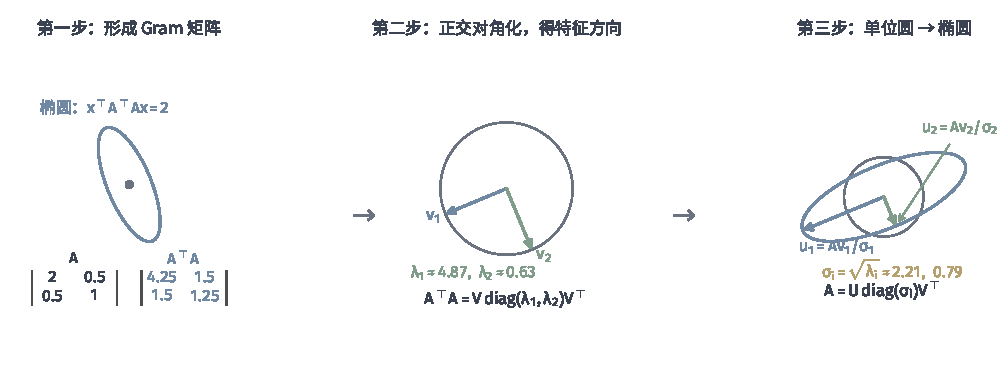
\includegraphics[width=168.998mm]{figures/01-mathematical-preliminaries-upper/03-linear-spaces/matplotlib/ls-svd-construction/ls-svd-construction.pdf}
  \caption{SVD 构造三部曲。以$\bm A=\left[\begin{smallmatrix}2&0.5\\0.5&1\end{smallmatrix}\right]$为例：
  (1)形成$\bm A^\top\bm A=\left[\begin{smallmatrix}4.25&1.5\\1.5&1.25\end{smallmatrix}\right]$；
  (2)由谱定理对角化，特征值$\lambda_1\approx4.87,\lambda_2\approx0.63$；
  (3)$\sigma_i=\sqrt{\lambda_i}\approx2.21,0.79$，右奇异向量$\bm v_i$即特征向量，
  左奇异向量$\bm u_i=\bm A\bm v_i/\sigma_i$。解析式教学构造。}
  \label{fig:ls-svd-construction}
\end{figure*}

几何上，$\bm A$把输入端的单位球面映成输出端的椭球面（秩亏时椭球退化）：$\bm v_i$方向的单位向量被送到长度为$\sigma_i$的半轴$\sigma_i\bm u_i$。图~\ref{fig:matrix-analysis-svd-geometry}用二维旋转矩阵$\bm R(\theta)=\left[\begin{smallmatrix}\cos\theta&-\sin\theta\\\sin\theta&\cos\theta\end{smallmatrix}\right]$构造了一个输入方向与输出方向不同的例子。

\begin{figure*}[htbp]
  \centering
  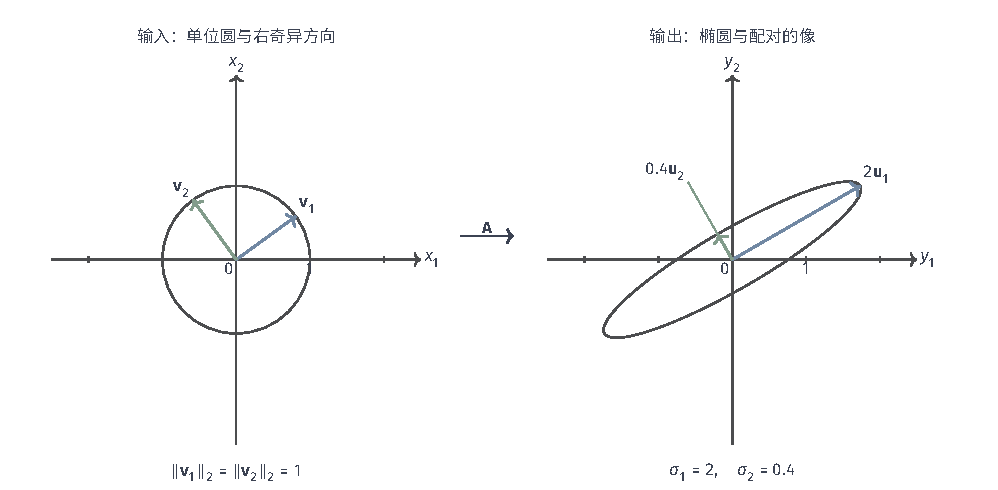
\includegraphics[width=168.998mm]{figures/01-mathematical-preliminaries-upper/03-linear-spaces/tikz/matrix-analysis-svd-geometry/figure.pdf}
  \caption{矩阵$\bm A=\bm R(\pi/6)\operatorname{diag}(2,0.4)\bm R(\pi/5)^\top$
  将单位圆变为椭圆。蓝、绿分别对应两个奇异方向；同色箭头在左侧标出$\bm v_i$，
  在右侧标出其像$\sigma_i\bm u_i$。两侧坐标比例相同。奇异值决定长度变化，左右方向可以不同，
  因而这不是沿特征方向的同空间缩放。图为教学构造。}
  \label{fig:matrix-analysis-svd-geometry}
\end{figure*}

奇异值由$\bm A$唯一确定，它们是$\bm A^\top\bm A$特征值的平方根。奇异向量则不唯一：$\sigma_i$重复时，对应子空间内的任意标准正交基都可以使用；单个$\sigma_i$的一对$\bm u_i,\bm v_i$也可以同时变号。

构造虽然从$\bm A^\top\bm A$出发，数值计算却并不真的形成它：$\bm A^\top\bm A$的特征值是$\sigma_i^2$，小奇异值平方后更小，在舍入中最先失去精度，第~\ref{chap:linear-equations-and-optimization}章讨论最小二乘的数值敏感性时会具体看到这一点。标准算法直接对$\bm A$从两侧施加正交变换，把它化为上双对角形，再迭代求出奇异值；只需要前几个奇异方向时，可以只计算相应的部分。

\subsection{奇异值与矩阵范数}

第~\ref{sec:ls-frobenius-norm}节与第~\ref{sec:ls-matrix-norms}节分别定义了Frobenius范数与谱范数，但没有给出谱范数的算法。SVD直接给出两者的值。对$\bm x=\sum_ic_i\bm v_i$，
\[
 \lVert\bm A\bm x\rVert_2^2=\sum_{i\leq r}\sigma_i^2c_i^2\leq\sigma_1^2\sum_ic_i^2=\sigma_1^2\lVert\bm x\rVert_2^2 ,
\]
等号在$\bm x=\bm v_1$时成立；而$\lVert\bm A\rVert_{\mathrm F}^2=\operatorname{tr}(\bm A^\top\bm A)$等于$\bm A^\top\bm A$的特征值之和$\sum_i\sigma_i^2$。因此
\begin{align}
 \lVert\bm A\rVert_2&=\sigma_1,
 \label{eq:matrix-analysis-spectral-norm}\\
 \lVert\bm A\rVert_{\mathrm F}&=\Bigl(\sum_{i=1}^r\sigma_i^2\Bigr)^{1/2}.
 \label{eq:matrix-analysis-frobenius-norm}
\end{align}
同一展开也给出最弱的放大。$d\leq m$时$\lVert\bm A\bm x\rVert_2\geq\sigma_d\lVert\bm x\rVert_2$，等号在$\bm x=\bm v_d$时成立，秩亏时$\sigma_d=0$。对可逆方阵，$\bm A^{-1}=\sum_i\sigma_i^{-1}\bm v_i\bm u_i^\top$（直接相乘可验证$\bm A\bm A^{-1}=\sum_i\bm u_i\bm u_i^\top=\bm I$），它的最大奇异值是$1/\sigma_d$，所以$\lVert\bm A^{-1}\rVert_2=1/\sigma_d$。

最大奇异值衡量最强的放大，最小奇异值衡量最弱的放大，二者之比就是第~\ref{sec:ls-perturbation-conditioning}节的条件数。齐次最小二乘~\eqref{eq:linear-algebra-homogeneous-least-squares}的最优解也可以由此读出：它是$\bm V$的最后一列$\bm v_d$，因为按构造，$\bm v_d$是$\bm A^\top\bm A$最小特征值的单位特征向量。

\subsection{极分解}

SVD还可以把方阵的作用分成“伸缩”与“转动”两步，类似于把复数写成模长与单位复数之积。设$\bm A\in\mathbb R^{d\times d}$有SVD$\bm A=\bm U\bm\Sigma\bm V^\top$，在$\bm U$与$\bm\Sigma$之间插入$\bm V^\top\bm V=\bm I$，得$\bm A=(\bm U\bm V^\top)(\bm V\bm\Sigma\bm V^\top)$。
\begin{definition}[极分解]
\label{def:matrix-analysis-polar-decomposition}
方阵$\bm A$的\term{极分解}（polar decomposition）是
\begin{equation}
 \bm A=\bm W\bm H,\qquad \bm W=\bm U\bm V^\top,\quad \bm H=\bm V\bm\Sigma\bm V^\top=(\bm A^\top\bm A)^{1/2},
 \label{eq:matrix-analysis-polar-decomposition}
\end{equation}
其中$\bm W$正交，$\bm H$对称半正定。
\end{definition}
$\bm H$先沿$\bm v_i$方向伸缩，$\bm W$再作正交变换。由$\bm H^2=\bm V\bm\Sigma^2\bm V^\top=\bm A^\top\bm A$及半正定平方根的唯一性，$\bm H$由$\bm A$唯一确定；$\bm A$可逆时$\bm H$可逆，$\bm W=\bm A\bm H^{-1}$也唯一。

正交因子$\bm W$是Frobenius范数下离$\bm A$最近的正交矩阵。对正交$\bm Z$，$\lVert\bm Z\rVert_{\mathrm F}^2=d$，展开得$\lVert\bm A-\bm Z\rVert_{\mathrm F}^2=\lVert\bm A\rVert_{\mathrm F}^2+d-2\operatorname{tr}(\bm Z^\top\bm A)$，所以只需让$\operatorname{tr}(\bm Z^\top\bm A)$最大。由迹的循环性，
\[
 \operatorname{tr}(\bm Z^\top\bm U\bm\Sigma\bm V^\top)=\operatorname{tr}(\bm V^\top\bm Z^\top\bm U\,\bm\Sigma)=\sum_i\sigma_i(\bm V^\top\bm Z^\top\bm U)_{i,i}.
\]
$\bm V^\top\bm Z^\top\bm U$是正交矩阵，其列是单位向量，对角元不超过$1$，故迹不超过$\sum_i\sigma_i$；取$\bm Z=\bm U\bm V^\top$时该矩阵为$\bm I$，等号成立。含噪的旋转估计常用这一步把近似正交的矩阵修正为正交矩阵。

\subsection{最佳低秩逼近}
\label{sec:ls-low-rank-solve}
\label{sec:ls-full-svd-solve}
\label{sec:matrix-analysis-svd-low-rank}

数据矩阵常常近似低秩：少数几个方向承载了大部分信息。给定秩上限$k$，怎样找离$\bm A$最近的秩不超过$k$的矩阵？秩一分解~\eqref{eq:matrix-analysis-svd-rank-one-sum}把$\bm A$按奇异值从大到小拆成$r$项，一个自然的候选是只保留前$k$项。

设$\bm A\in\mathbb R^{m\times d}$的非零奇异值为$\sigma_1\geq\cdots\geq\sigma_r>0$，称
\begin{equation}
 \bm A_k=\sum_{i=1}^k\sigma_i\bm u_i\bm v_i^\top,
 \qquad 0\leq k<r
 \label{eq:matrix-analysis-truncated-svd}
\end{equation}
为\term{截断SVD}（truncated SVD），$k=0$时$\bm A_0=\bm0$。

余下的$\bm A-\bm A_k=\sum_{i>k}\sigma_i\bm u_i\bm v_i^\top$本身就是一个SVD，最大奇异值为$\sigma_{k+1}$，由式~\eqref{eq:matrix-analysis-spectral-norm}与式~\eqref{eq:matrix-analysis-frobenius-norm}直接读出两种误差：
\begin{equation}
 \lVert\bm A-\bm A_k\rVert_2=\sigma_{k+1},\qquad
 \lVert\bm A-\bm A_k\rVert_{\mathrm F}
 =\Bigl(\sum_{i=k+1}^r\sigma_i^2\Bigr)^{1/2}.
 \label{eq:ls-truncated-errors}
\end{equation}
谱范数误差是最坏单位输入的输出偏差，Frobenius误差累计全部元素的平方偏差。下面的定理说明，在这两种范数下没有比截断SVD更好的秩$k$近似。

\begin{theorem}[Eckart--Young--Mirsky最佳低秩逼近]
\label{thm:ls-best-low-rank}
\label{thm:matrix-analysis-best-low-rank}
对$0\leq k<r=\operatorname{rank}\bm A$，
\begin{align}
 \min_{\operatorname{rank}\bm B\leq k}\lVert\bm A-\bm B\rVert_2
 &=\sigma_{k+1},
 \label{eq:matrix-analysis-best-rank-k-spectral}\\
 \min_{\operatorname{rank}\bm B\leq k}\lVert\bm A-\bm B\rVert_{\mathrm F}
 &=\Bigl(\sum_{i=k+1}^r\sigma_i^2\Bigr)^{1/2},
 \label{eq:matrix-analysis-best-rank-k-frobenius}
\end{align}
两个最小值都由截断SVD$\bm A_k$达到。
\end{theorem}
\begin{proof}
式~\eqref{eq:ls-truncated-errors}说明$\bm A_k$达到右端，只需证明任意秩不超过$k$的$\bm B$误差都不更小。$k=0$时$\bm B=\bm0$，结论即式~\eqref{eq:ls-truncated-errors}，下设$k\geq1$。

谱范数情形。$\ker\bm B$的维数至少为$d-k$，子空间$\operatorname{span}\{\bm v_1,\ldots,\bm v_{k+1}\}$的维数为$k+1$，两者维数之和超过$d$，必有公共单位向量$\bm x=\sum_{i=1}^{k+1}c_i\bm v_i$，$\sum_ic_i^2=1$。由$\bm B\bm x=\bm0$，
\begin{equation}
 \lVert(\bm A-\bm B)\bm x\rVert_2
 =\lVert\bm A\bm x\rVert_2
 =\Bigl(\sum_{i=1}^{k+1}\sigma_i^2c_i^2\Bigr)^{1/2}
 \geq\sigma_{k+1},
 \label{eq:ls-spectral-lower-bound}
\end{equation}
所以$\lVert\bm A-\bm B\rVert_2\geq\sigma_{k+1}$。

Frobenius情形。正交变换不改变Frobenius范数，令$\bm C=\bm U^\top\bm B\bm V$，则$\operatorname{rank}\bm C=\operatorname{rank}\bm B\leq k$，且$\lVert\bm A-\bm B\rVert_{\mathrm F}=\lVert\bm\Sigma-\bm C\rVert_{\mathrm F}$。设$\bm P$为到$\bm C$列空间的正交投影，则$\operatorname{tr}\bm P=\operatorname{rank}\bm C\leq k$，且$\bm P\bm C=\bm C$。把$\bm\Sigma-\bm C$拆成$(\bm I-\bm P)\bm\Sigma$与$\bm P\bm\Sigma-\bm C$，两部分的每一列分别落在互相正交的子空间中，于是
\[
 \lVert\bm\Sigma-\bm C\rVert_{\mathrm F}^2
 =\lVert(\bm I-\bm P)\bm\Sigma\rVert_{\mathrm F}^2+\lVert\bm P\bm\Sigma-\bm C\rVert_{\mathrm F}^2
 \geq\lVert\bm\Sigma\rVert_{\mathrm F}^2-\lVert\bm P\bm\Sigma\rVert_{\mathrm F}^2 .
\]
$\bm\Sigma$的第$i$列是$\sigma_i\bm e_i$，所以保留部分为$\lVert\bm P\bm\Sigma\rVert_{\mathrm F}^2=\sum_i\sigma_i^2w_i$，其中$w_i=\lVert\bm P\bm e_i\rVert_2^2\in[0,1]$，且$\sum_iw_i\leq\lVert\bm P\rVert_{\mathrm F}^2=\operatorname{tr}\bm P\leq k$。与迹极值定理的证明相同，由$\sigma_i$降序，
\[
 \sum_i\sigma_i^2w_i-\sum_{i\leq k}\sigma_i^2
 =\sum_{i\leq k}\sigma_i^2(w_i-1)+\sum_{i>k}\sigma_i^2w_i
 \leq\sigma_k^2\Bigl(\sum_iw_i-k\Bigr)\leq0 .
\]
即保留部分不超过$\sum_{i\leq k}\sigma_i^2$，误差平方至少为$\lVert\bm\Sigma\rVert_{\mathrm F}^2-\sum_{i\leq k}\sigma_i^2=\sum_{i>k}\sigma_i^2$。
\end{proof}
这一结论最早由Eckart与Young给出\scite{eckart1936}。上面的证明只处理谱范数与Frobenius范数；误差改用加权、逐元素或分组的度量时，最优性需要重新论证，截断SVD一般不再是最优解。图~\ref{fig:ls-low-rank-truncation}画出截断的几何：单位圆经$\bm A$变成椭圆，秩一近似把椭圆压成主轴方向的线段，残留误差恰为舍弃的$\sigma_2$。

\begin{figure*}[htbp]
  \centering
  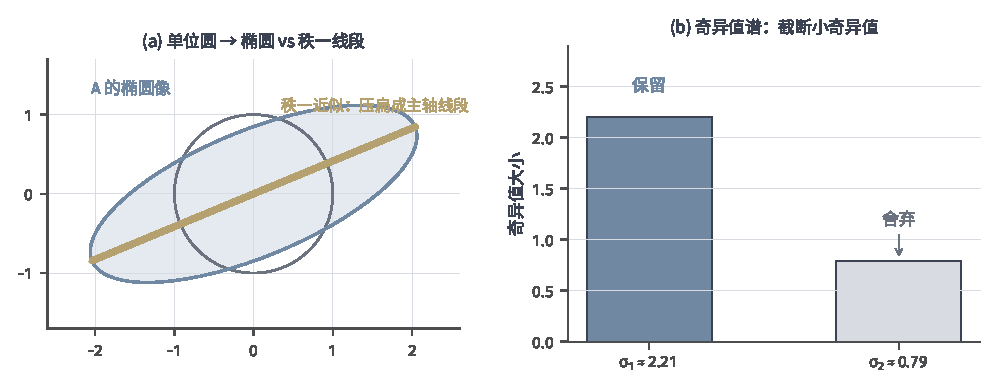
\includegraphics[width=168.998mm]{figures/01-mathematical-preliminaries-upper/03-linear-spaces/matplotlib/ls-low-rank-truncation/ls-low-rank-truncation.pdf}
  \caption{低秩截断的几何。$\bm A=\left[\begin{smallmatrix}2&0.5\\0.5&1\end{smallmatrix}\right]$，
  灰圆为单位圆，蓝椭圆为$\bm A$的像。左：黄粗线段为秩一近似$\bm A_1=\sigma_1\bm v_1\bm v_1^\top$
  的像，椭圆被压成长$2\sigma_1$的线段；右：$\sigma_1\approx2.21$（保留）、$\sigma_2\approx0.79$
  （舍弃），算子范数误差$\lVert\bm A-\bm A_1\rVert_2=\sigma_2$。$\sigma_{1,2}=(3\pm\sqrt2)/2$。
  固定复算。}
  \label{fig:ls-low-rank-truncation}
\end{figure*}

回到本节开头的问题：任意矩阵都能写成$\bm A=\sum_{i\leq r}\sigma_i\bm u_i\bm v_i^\top$，在输入、输出两侧各取一组标准正交方向后，它只是逐个方向的伸缩。奇异值由$\bm A$唯一确定，最大奇异值是谱范数，平方和是Frobenius范数的平方，最小奇异值衡量最弱的放大；方阵还可以写成正交因子与半正定因子之积；按奇异值从大到小截断，得到谱范数与Frobenius范数下的最佳低秩逼近。同一个和式还能反过来用：把每一项$\sigma_i\bm u_i\bm v_i^\top$换成$\sigma_i^{-1}\bm v_i\bm u_i^\top$，就得到秩亏、不相容方程的最小范数最小二乘解，这一构造留到第~\ref{chap:linear-equations-and-optimization}章与线性方程的求解一起讨论。

到这里，本章的第一个问题告一段落：由特征向量组成的基（若存在）使算子的矩阵成为对角形；要求基标准正交时，对称矩阵仍能对角化，一般方阵只能化为实Schur形；输入、输出各取一组标准正交基时，任意矩阵都能对角化。后面三节用这些最简形式研究线性作用的性质，首先是一次作用对误差的放大。最强与最弱的放大分别由最大与最小奇异值给出，下一节用它们定义条件数。

% 第6章第6节：条件数（输入、输出与误差，条件数的定义，基本运算的敏感度）。

\section{条件数}
\label{sec:ls-perturbation}
\label{sec:linear-algebra-stability}
\label{sec:matrix-analysis-conditioning-perturbation}

前五节为线性作用找到了最简形式。从本节起，用这些形式研究线性作用的性质，首先是它对误差的反应。实际交给计算的数据总带误差：测量有噪声，记录有截断，上一步计算有舍入。数据与理想输入相差一点时，答案相差多少？允许范围内的输入增量称为\term{扰动}（perturbation）。扰动分析不改变任务本身，只测量输入的增量在输出中被放大多少倍。

本节先确定怎样度量输入与输出的误差，再定义衡量最坏放大倍数的条件数，说明矩阵的条件数就是最大与最小奇异值之比，最后用同样的增量展开检查几种基本运算。线性方程与最小二乘的解对数据的敏感度，要等第~\ref{chap:linear-equations-and-optimization}章建立求解方法之后，再用本节的工具讨论。

\subsection{输入、输出与误差}

为了统一讨论，把任务看作映射$F$：理想输入$\bm z$对应输出$F(\bm z)$，实际输入为$\bm z+\Delta\bm z$，输出增量为
\[
 \Delta\bm y=F(\bm z+\Delta\bm z)-F(\bm z).
\]
任务不同，比较的输出也不同：矩阵乘向量比较输出向量，求逆比较逆矩阵，解方程比较解向量，谱分解要分别比较特征值与特征子空间。这里只改变数据，不更换算法；算法在机器上产生的舍入误差是另一个来源，第~\ref{chap:linear-equations-and-optimization}章讨论线性方程的数值敏感性时再单独处理。

衡量增量大小有两种方式。\term{绝对误差}（absolute error）直接取增量的范数$\lVert\Delta\bm z\rVert$、$\lVert\Delta\bm y\rVert$。当输入与输出本身有尺度时，更常用\term{相对误差}（relative error）
\[
 \frac{\lVert\Delta\bm z\rVert}{\lVert\bm z\rVert},
 \qquad
 \frac{\lVert\Delta\bm y\rVert}{\lVert F(\bm z)\rVert}.
\]
相对误差在整体缩放下不变，反映变化占原有量的比例；但输出接近零时它失去意义，应改报绝对误差。

误差读数还依赖范数与允许改变的分量：只改右端、同时改矩阵与右端、要求扰动保持对称，是三个不同的扰动问题，敏感度一般不同。

\subsection{条件数的定义}
\label{sec:ls-perturbation-conditioning}

输入增量可以朝任意允许的方向取，敏感度应由最坏方向决定。对足够小的增量，取输出增量与输入增量之比的上确界，
\[
 \kappa_{\mathrm{abs}}(F;\bm z)
 =\lim_{\delta\to0}\ \sup_{0<\lVert\Delta\bm z\rVert\leq\delta}
 \frac{\lVert F(\bm z+\Delta\bm z)-F(\bm z)\rVert}
      {\lVert\Delta\bm z\rVert},
\]
称为任务$F$在$\bm z$处的\term{绝对条件数}（absolute condition number）。对线性作用$\bm x\mapsto\bm A\bm x$，输出增量是$\bm A\Delta\bm x$，增量之比$\lVert\bm A\Delta\bm x\rVert/\lVert\Delta\bm x\rVert$只依赖$\Delta\bm x$的方向，与$\bm x$和$\delta$无关。所以绝对条件数就是第~\ref{sec:ls-matrix-norms}节的诱导范数$\lVert\bm A\rVert$，在最大放大方向达到。

图~\ref{fig:ls-condition-number-amplification}把单位圆与误差圆盘分别送进两个矩阵：良态矩阵的像接近圆，病态矩阵的像被拉成细条，同样半径的误差圆盘反求后沿最弱方向被放大许多倍。

\begin{figure*}[htbp]
 \centering
 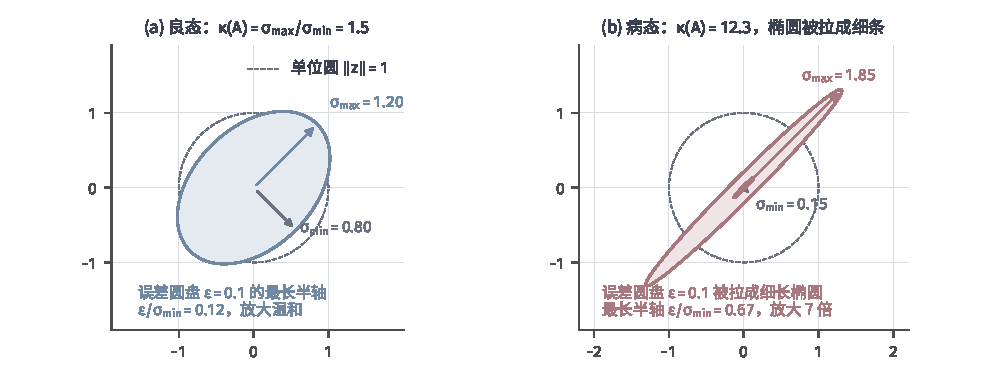
\includegraphics[width=169.0mm]{figures/01-mathematical-preliminaries-upper/03-linear-spaces/matplotlib/ls-condition-number-amplification/ls-condition-number-amplification.pdf}
 \caption{条件数对误差圆盘的放大。灰虚线为单位圆$\lVert\bm z\rVert=1$；左为良态
 $\bm A_1=[[1,0.2],[0.2,1]]$，奇异值$1.20$与$0.80$，$\kappa_2=1.5$，像椭圆接近
 圆；右为病态$\bm A_2=[[1,0.85],[0.85,1]]$，奇异值$1.85$与$0.15$，$\kappa_2\approx12.3$，
 像被拉成细条。半径$\varepsilon=0.1$的误差圆盘（红）最长半轴为$\varepsilon/\sigma_{\min}$：
 良态为$0.125$，病态约$0.67$。}
 \label{fig:ls-condition-number-amplification}
\end{figure*}

把输入、输出都换成相对尺度，得到\term{相对条件数}（relative condition number）
\[
 \kappa_{\mathrm{rel}}(F;\bm z)
 =\lim_{\delta\to0}\ \sup_{0<\lVert\Delta\bm z\rVert\leq\delta}
 \frac{\lVert\Delta\bm y\rVert/\lVert F(\bm z)\rVert}
      {\lVert\Delta\bm z\rVert/\lVert\bm z\rVert}.
\]
对线性作用，$\kappa_{\mathrm{rel}}(\bm A;\bm x)=\lVert\bm A\rVert\lVert\bm x\rVert/\lVert\bm A\bm x\rVert$随$\bm x$变化：$\bm x$落在被压缩的方向上时，输出$\bm A\bm x$小，相对条件数大；落在主伸缩方向上时它小。对可逆方阵再对所有$\bm x$取最坏，令$\bm y=\bm A\bm x$，
\[
 \sup_{\bm x\neq\bm0}\frac{\lVert\bm A\rVert\lVert\bm x\rVert}{\lVert\bm A\bm x\rVert}
 =\lVert\bm A\rVert\sup_{\bm y\neq\bm0}\frac{\lVert\bm A^{-1}\bm y\rVert}{\lVert\bm y\rVert}
 =\lVert\bm A\rVert\,\lVert\bm A^{-1}\rVert ,
\]
这个只依赖矩阵的数就是矩阵的条件数。

\begin{definition}[可逆矩阵的条件数]
\label{def:matrix-analysis-condition-number}
对同一向量范数诱导的矩阵范数，可逆方阵$\bm A$的\term{条件数}（condition number）为
\begin{equation}
 \kappa(\bm A)=\lVert\bm A\rVert\,\lVert\bm A^{-1}\rVert .
 \label{eq:matrix-analysis-condition-number}
\end{equation}
\end{definition}
由第~\ref{sec:ls-svd}节，欧氏范数下$\lVert\bm A\rVert_2=\sigma_{\max}$、$\lVert\bm A^{-1}\rVert_2=1/\sigma_{\min}$，故
\begin{equation}
 \kappa_2(\bm A)=\frac{\sigma_{\max}(\bm A)}{\sigma_{\min}(\bm A)},
 \label{eq:matrix-analysis-spectral-condition-number}
\end{equation}
即最强放大与最弱放大之比。条件数总不小于$1$，因为$1=\lVert\bm I\rVert=\lVert\bm A\bm A^{-1}\rVert\leq\lVert\bm A\rVert\lVert\bm A^{-1}\rVert=\kappa(\bm A)$。正交矩阵的奇异值全为$1$，所以$\kappa_2=1$。矩阵接近奇异时$\sigma_{\min}\to0$，$\kappa_2$增大，与图~\ref{fig:ls-condition-number-amplification}右侧的细长椭圆一致。条件数接近$1$的问题称为良态，条件数很大的问题称为病态。

\begin{theorem}[条件数基本界]
\label{thm:matrix-analysis-condition-number-bound}
设$\kappa(F;\bm z)$为任务$F$在$\bm z$处的相对条件数，则足够小的输入扰动满足
\begin{equation}
 \frac{\lVert\Delta\bm y\rVert}{\lVert F(\bm z)\rVert}
 \lesssim\kappa(F;\bm z)\,\frac{\lVert\Delta\bm z\rVert}{\lVert\bm z\rVert}.
 \label{eq:matrix-analysis-condition-number-bound}
\end{equation}
特别地，可逆系统$\bm A\bm x=\bm b$的右端扰动$\Delta\bm b$引起的解扰动对任意大小的$\Delta\bm b$都满足$\lVert\Delta\bm x\rVert/\lVert\bm x\rVert\leq\kappa(\bm A)\lVert\Delta\bm b\rVert/\lVert\bm b\rVert$。
\end{theorem}
\begin{proof}
第一式是相对条件数定义的直接改写，$\lesssim$表示忽略比$\lVert\Delta\bm z\rVert$高阶的小量。对方程，$\bm A(\bm x+\Delta\bm x)=\bm b+\Delta\bm b$减去$\bm A\bm x=\bm b$，得$\Delta\bm x=\bm A^{-1}\Delta\bm b$，故$\lVert\Delta\bm x\rVert\leq\lVert\bm A^{-1}\rVert\lVert\Delta\bm b\rVert$；又$\lVert\bm b\rVert=\lVert\bm A\bm x\rVert\leq\lVert\bm A\rVert\lVert\bm x\rVert$，即$1/\lVert\bm x\rVert\leq\lVert\bm A\rVert/\lVert\bm b\rVert$。两式相乘即得。
\end{proof}

条件数是最坏方向上的上界，不是每个扰动都达到的倍数。一般任务的相对条件数只控制足够小的扰动；矩阵本身的扰动较大时，还要考虑扰动后是否仍然可逆，这在第~\ref{chap:linear-equations-and-optimization}章估计逆矩阵与方程解的敏感度时处理。

条件数也不回答反复作用的长期结果。下面的反例中，两个矩阵的条件数相同，幂的变化趋势却相反。
\begin{example}[反例：条件数相同而幂的趋势相反]
\label{ex:ls-condition-number-vs-powers}
给定同阶的$2\bm I$与$\tfrac12\bm I$。二者的奇异值分别全为$2$与全为$\tfrac12$，所以
\[
 \kappa_2(2\bm I)=\frac{2}{2}=1,\qquad
 \kappa_2\bigl(\tfrac12\bm I\bigr)=\frac{1/2}{1/2}=1 .
\]
但$(2\bm I)^k=2^k\bm I$逐次增长，$(\tfrac12\bm I)^k=2^{-k}\bm I$逐次衰减。结论：条件数相同的两个矩阵，反复作用的结果可以完全相反。
\end{example}
条件数衡量一次作用的相对放大，长期行为要由谱半径判断（第~\ref{sec:ls-matrix-power-behavior}节），二者不能互相代替。

\subsection{基本运算的敏感度}

同样的增量展开适用于第~\ref{chap:linear-operations}章的基本运算。先看加法。和的增量是$\Delta(\bm x+\bm y)=\Delta\bm x+\Delta\bm y$，由三角不等式，$\lVert\Delta(\bm x+\bm y)\rVert\leq\lVert\Delta\bm x\rVert+\lVert\Delta\bm y\rVert$，所以加法本身不放大绝对误差。但$\bm x\approx-\bm y$时理想输出很小，相对误差被小分母放大，下面的例子给出具体数值。
\begin{example}[加法中的抵消]
\label{ex:ls-cancellation-relative-error}
给定$x=1.0001$、$y=-1.0000$，二者各带至多$5\times10^{-5}$的绝对误差，相对误差约为$5\times10^{-5}$。理想和为$x+y=10^{-4}$，而和的绝对误差至多为$5\times10^{-5}+5\times10^{-5}=10^{-4}$，所以和的相对误差可达
\[
 \frac{10^{-4}}{10^{-4}}=1 .
\]
结论：输入的相对误差约为$5\times10^{-5}$，输出的相对误差却可达$1$，放大约$2\times10^4$倍。
\end{example}
这种抵消不是算法失误，而是问题本身在相对尺度下病态。

再看乘积。它满足
\[
 (\bm A+\bm E)(\bm B+\bm F)-\bm A\bm B=\bm A\bm F+\bm E\bm B+\bm E\bm F,
\]
前两项是一阶响应，各被另一个因子的范数放大，末项在小扰动下是二阶量。

最后看行列式，它在矩阵接近奇异时最敏感。
\begin{example}[接近奇异时的行列式]
\label{ex:ls-determinant-near-singular}
给定$\bm A=\operatorname{diag}(1,\varepsilon)$，$0<\varepsilon<1$，则$\det\bm A=\varepsilon$。把第二个对角元改为$\varepsilon+\delta$，矩阵的相对变化为$\lVert\Delta\bm A\rVert_2/\lVert\bm A\rVert_2=|\delta|$，行列式变为$\varepsilon+\delta$，相对变化为
\[
 \frac{|(\varepsilon+\delta)-\varepsilon|}{\varepsilon}=\frac{|\delta|}{\varepsilon}.
\]
结论：行列式的相对误差是矩阵相对误差的$1/\varepsilon$倍，矩阵越接近奇异，放大越强。
\end{example}

本节得到的结论是：条件数$\kappa(\bm A)=\lVert\bm A\rVert\lVert\bm A^{-1}\rVert$是一次作用下相对误差的最坏放大倍数，欧氏范数下等于$\sigma_{\max}/\sigma_{\min}$，在各方向伸缩悬殊、矩阵接近奇异时变大；加法在抵消时、行列式在矩阵接近奇异时，相对误差也会被小分母放大。这里矩阵始终是固定的，只有输入向量带误差。可是矩阵本身也常常来自数据，例如由有限样本估计的协方差矩阵。下一节把矩阵当作输入，研究它的特征值、奇异值与特征子空间对扰动的敏感度。

% 第6章第7节：谱的扰动（特征值与奇异值的移动、子空间之间的距离、特征子空间的转动）。

\section{谱的扰动}
\label{sec:ls-spectral-sensitivity}
\label{sec:linear-algebra-spectral-stability}
\label{sec:ch06-spectral-stability}

上一节让矩阵保持不变，只扰动输入向量。实际中矩阵本身也来自数据：协方差矩阵由有限样本估计，系数矩阵经过测量和舍入。这时谱分解的输入是矩阵，输出有两类：特征值（或奇异值）与特征子空间（或奇异子空间）。矩阵受到扰动$\bm E$后，它们分别移动多少？

本节先证明对称矩阵的特征值与任意矩阵的奇异值移动不超过$\lVert\bm E\rVert_2$，并说明非对称矩阵的特征值为何没有这样的保证；再建立一个与基的选取无关的子空间距离；最后证明特征子空间转过的角度由扰动与特征值间隔之比控制。

\subsection{特征值与奇异值的移动}
\label{sec:ls-spectral-value-sensitivity}

先看特征值。实对称矩阵的特征值全为实数，可以把扰动前后的特征值都按降序排列，记为$\lambda_1\geq\cdots\geq\lambda_d$与$\widetilde\lambda_1\geq\cdots\geq\widetilde\lambda_d$，再按同一次序逐个比较。对正定矩阵$\bm A$，椭圆$\{\bm x:\bm x^\top\bm A\bm x\leq1\}$的主轴沿特征方向，半轴长为$1/\sqrt\lambda$。图~\ref{fig:ls-perturbation-ellipse}画出$\bm A$换成$\bm A+\bm E$前后的两个椭圆：半轴长微变，主轴微转。

\begin{figure}[htbp]
 \centering
 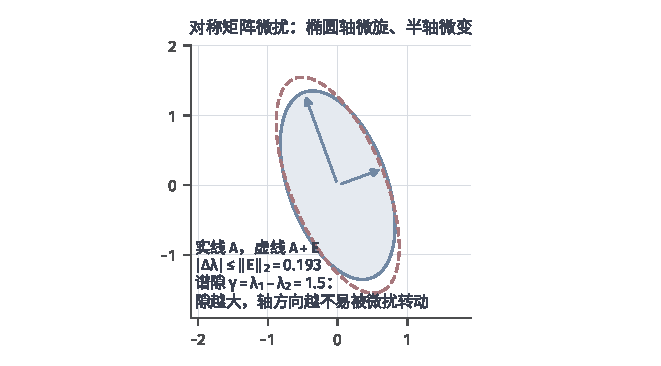
\includegraphics[width=112mm]{figures/01-mathematical-preliminaries-upper/03-linear-spaces/matplotlib/ls-perturbation-ellipse/ls-perturbation-ellipse.pdf}
 \caption{对称矩阵微扰的谱与方向。实线椭圆为$\bm A$（特征值$2$与$0.5$，主轴
 方向$20^\circ$），虚线为$\bm A+\bm E$（$\lVert\bm E\rVert_2\approx0.193$）：轴
 微旋、半轴微变。新特征值约$2.18$与$0.37$，偏移$0.18$、$0.13$均小于
 $\lVert\bm E\rVert_2$，符合Weyl界；未扰动的谱隙$\delta=\lambda_1-\lambda_2=1.5$越大，
 特征方向越不易被微扰转动。}
 \label{fig:ls-perturbation-ellipse}
\end{figure}

Courant--Fischer定理把每个特征值写成Rayleigh商的最小最大值，而扰动$\bm E$对Rayleigh商的影响不超过$\lVert\bm E\rVert_2$，由此得到下面的界。
\begin{theorem}[Weyl特征值扰动界]
\label{thm:ls-weyl-eigenvalue}
对实对称$\bm A,\bm E\in\mathbb R^{d\times d}$，$\widetilde{\bm A}=\bm A+\bm E$与$\bm A$按降序配对的特征值满足
\begin{equation}
 |\widetilde\lambda_k-\lambda_k|
 \leq\lVert\bm E\rVert_2,
 \qquad k=1,\dots,d.
 \label{eq:matrix-analysis-weyl-eigenvalue-perturbation}
\end{equation}
\end{theorem}
\begin{proof}
$\bm E$对称，由Rayleigh--Ritz定理，它的Rayleigh商介于最小与最大特征值之间，而它们的绝对值不超过$\lVert\bm E\rVert_2$，所以$|\bm x^\top\bm E\bm x|\leq\lVert\bm E\rVert_2\lVert\bm x\rVert_2^2$。取$\mathcal V=\operatorname{span}\{\bm q_1,\ldots,\bm q_k\}$（$\bm A$的前$k$个特征向量），其中每个$\bm x$满足
\[
 \bm x^\top\widetilde{\bm A}\bm x=\bm x^\top\bm A\bm x+\bm x^\top\bm E\bm x\geq(\lambda_k-\lVert\bm E\rVert_2)\lVert\bm x\rVert_2^2 .
\]
由Courant--Fischer定理，$\widetilde\lambda_k$不小于$\widetilde{\bm A}$在任一$k$维子空间上Rayleigh商的最小值，故$\widetilde\lambda_k\geq\lambda_k-\lVert\bm E\rVert_2$。把$\widetilde{\bm A}$看作$\bm A$加扰动$-\bm E$，交换二者的角色得$\lambda_k\geq\widetilde\lambda_k-\lVert\bm E\rVert_2$。
\end{proof}

Weyl界不需要特征值彼此分开，单重与重复特征值都适用。

Weyl界也给出奇异值的稳定性。把$\bm A\in\mathbb R^{m\times d}$嵌入对称分块矩阵$\left[\begin{smallmatrix}\bm0&\bm A\\\bm A^\top&\bm0\end{smallmatrix}\right]$，由$\bm A\bm v_i=\sigma_i\bm u_i$、$\bm A^\top\bm u_i=\sigma_i\bm v_i$可直接验证向量$(\bm u_i,\pm\bm v_i)$是它的特征向量，特征值为$\pm\sigma_i$，其余特征值为零；而$\bm E$嵌入后谱范数不变。对嵌入矩阵应用Weyl界，得
\begin{equation}
 |\widetilde\sigma_i-\sigma_i|\leq\lVert\bm E\rVert_2 .
 \label{eq:matrix-analysis-singular-value-perturbation}
\end{equation}
截断SVD的误差$\sigma_{k+1}$（定理~\ref{thm:ls-best-low-rank}）因而也只移动不超过$\lVert\bm E\rVert_2$。

非对称矩阵的特征值没有这样的保证。设$\bm A=\bm V\bm\Lambda\bm V^{-1}$可对角化，$\mu$是$\bm A+\bm E$的特征值而不是$\bm A$的特征值，$\bm w$为对应的特征向量（必要时取复数）。由$(\bm A+\bm E)\bm w=\mu\bm w$，令$\bm y=\bm V^{-1}\bm w\neq\bm0$，得$(\bm\Lambda-\mu\bm I)\bm y=-\bm V^{-1}\bm E\bm V\bm y$。$\mu$不是$\bm A$的特征值，所以对角矩阵$\bm\Lambda-\mu\bm I$可逆，于是$\bm y=-(\bm\Lambda-\mu\bm I)^{-1}\bm V^{-1}\bm E\bm V\bm y$。两边取范数并除以$\lVert\bm y\rVert_2$，得$1\leq\lVert(\bm\Lambda-\mu\bm I)^{-1}\rVert_2\,\kappa_2(\bm V)\lVert\bm E\rVert_2$；而对角矩阵$(\bm\Lambda-\mu\bm I)^{-1}$的范数是$1/\min_k|\lambda_k-\mu|$，于是得到Bauer--Fike界
\[
 \min_k|\mu-\lambda_k|\leq\kappa_2(\bm V)\lVert\bm E\rVert_2 .
\]
特征向量越接近线性相关，$\kappa_2(\bm V)$越大，界越宽。对称情形$\bm V$可取正交矩阵，$\kappa_2(\bm V)=1$，界与Weyl界同量级。

不可对角化时情况更糟，特征值的移动可以远大于扰动本身。
\begin{example}[反例：特征值的移动远大于扰动]
\label{ex:ls-jordan-eigenvalue-sensitivity}
给定$\bm N=\left[\begin{smallmatrix}0&1\\0&0\end{smallmatrix}\right]$，它的特征值全为$0$。在左下角加入扰动$\varepsilon$，得
\[
 \bm N_\varepsilon=\begin{bmatrix}0&1\\\varepsilon&0\end{bmatrix},\qquad
 p_{\bm N_\varepsilon}(z)=z^2-\varepsilon ,
\]
扰动的大小为$\lVert\bm N_\varepsilon-\bm N\rVert_2=|\varepsilon|$。$\varepsilon>0$时特征值为$\pm\sqrt\varepsilon$，移动量为$\sqrt\varepsilon$；例如$\varepsilon=10^{-10}$时特征值移动$10^{-5}$，是扰动的$10^5$倍。$\varepsilon<0$时特征值为$\pm\mathrm i\sqrt{|\varepsilon|}$，实特征值消失。结论：特征值的移动量是$O(\sqrt{|\varepsilon|})$而非$O(|\varepsilon|)$，不能由扰动的范数乘一个常数控制。
\end{example}
可见对非对称矩阵，特征值的敏感程度取决于矩阵的结构：可对角化时，移动量至多是扰动的$\kappa_2(\bm V)$倍；不可对角化时，移动量甚至不与扰动成正比。

\subsection{子空间之间的距离}
\label{sec:ls-subspace-sensitivity}

比较特征向量时先要确定比较什么。同一子空间的基可以旋转、变号，单个基向量的变化不能当作子空间误差；特征值重复时，特征空间内部怎么换基都不改变子空间。所以比较对象必须是子空间本身，需要一个与基的选取无关的度量。图~\ref{fig:ls-principal-angles-subspaces}从两条过原点的直线看起：两直线的夹角与方向向量的选取无关；把一条直线的单位方向向量投影到另一条上，投影不掉的部分长度为$\sin\theta$。

\begin{figure}[htbp]
 \centering
 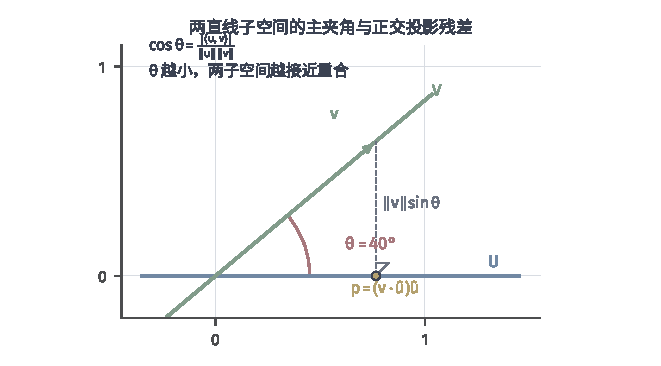
\includegraphics[width=112mm]{figures/01-mathematical-preliminaries-upper/03-linear-spaces/matplotlib/ls-principal-angles-subspaces/ls-principal-angles-subspaces.pdf}
 \caption{两条直线子空间的主夹角。蓝线为$\bm U$、绿线为$\bm V$，红弧为主夹角
 $\theta=40^\circ$；黄点$\bm p$是$\bm v$在$\bm U$上的正交投影，灰虚线为投影
 垂线。$\cos40^\circ\approx0.766$、$\sin40^\circ\approx0.643$，残差长度
 $\lVert\bm v\rVert\sin\theta$即投影不掉的分量。}
 \label{fig:ls-principal-angles-subspaces}
\end{figure}

对一维子空间，若$\bm q,\widetilde{\bm q}$是单位方向向量，则$|\bm q^\top\widetilde{\bm q}|=\cos\theta$。高维子空间之间有多个夹角，由交叉内积矩阵的奇异值给出。
\begin{definition}[主夹角]
\label{def:matrix-analysis-principal-angles}
设$\bm Q,\widetilde{\bm Q}\in\mathbb R^{d\times r}$列标准正交，分别张成$r$维子空间。交叉矩阵$\bm Q^\top\widetilde{\bm Q}$的奇异值记为$\cos\theta_1\geq\dots\geq\cos\theta_r$，$0\leq\theta_1\leq\cdots\leq\theta_r\leq\pi/2$，这些$\theta_i$称为两个子空间的\term{主夹角}（principal angles）。
\end{definition}
这些奇异值都在$[0,1]$内，因为$\lVert\bm Q^\top\widetilde{\bm Q}\rVert_2\leq\lVert\bm Q\rVert_2\lVert\widetilde{\bm Q}\rVert_2=1$，所以$\theta_i$有定义。换基相当于把$\bm Q$、$\widetilde{\bm Q}$右乘正交矩阵，交叉矩阵的奇异值不变，所以主夹角只依赖子空间。

主夹角的正弦也可以直接读出。设$\widetilde{\bm Q}_\perp$的列是$\widetilde{\bm Q}$列空间正交补的标准正交基。对单位向量$\bm a$，把$\bm Q\bm a$分解到$\widetilde{\bm Q}$的列空间与其正交补，由勾股定理，
\[
 \lVert\widetilde{\bm Q}^\top\bm Q\bm a\rVert_2^2+\lVert\widetilde{\bm Q}_\perp^\top\bm Q\bm a\rVert_2^2=\lVert\bm Q\bm a\rVert_2^2=1 .
\]
记$\bm C=\widetilde{\bm Q}^\top\bm Q$、$\bm X=\widetilde{\bm Q}_\perp^\top\bm Q$。上式对所有单位向量$\bm a$成立，说明对称矩阵$\bm X^\top\bm X$与$\bm I-\bm C^\top\bm C$的二次型处处相等，所以$\bm X^\top\bm X=\bm I-\bm C^\top\bm C$。$\bm C$是交叉矩阵的转置，奇异值为$\cos\theta_i$，所以$\bm X^\top\bm X$的特征值是$1-\cos^2\theta_i=\sin^2\theta_i$，即$\bm X$的奇异值是$\sin\theta_i$。

子空间的误差还可以用正交投影$\bm P=\bm Q\bm Q^\top$、$\widetilde{\bm P}=\widetilde{\bm Q}\widetilde{\bm Q}^\top$之差表示，它与基的选取无关。可以证明
\[
 \lVert\bm P-\widetilde{\bm P}\rVert_2=\sin\theta_r,\qquad
 \tfrac12\lVert\bm P-\widetilde{\bm P}\rVert_{\mathrm F}^2=\sum_{i=1}^r\sin^2\theta_i .
\]
第二式可以直接验证：由$\operatorname{tr}\bm P=\operatorname{tr}\widetilde{\bm P}=r$与$\operatorname{tr}(\bm P\widetilde{\bm P})=\lVert\bm Q^\top\widetilde{\bm Q}\rVert_{\mathrm F}^2=\sum_i\cos^2\theta_i$，得$\lVert\bm P-\widetilde{\bm P}\rVert_{\mathrm F}^2=2r-2\sum_i\cos^2\theta_i=2\sum_i\sin^2\theta_i$。第一式说明投影矩阵之差的谱范数就是最大主夹角的正弦，它的证明较长，这里从略。

\subsection{特征子空间的转动}

有了主夹角，就可以估计扰动使特征子空间转过多大的角度。设$\bm A$、$\widetilde{\bm A}=\bm A+\bm E$实对称，$\bm Q$的列是$\bm A$的前$k$个单位特征向量，$\widetilde{\bm Q}$的列是$\widetilde{\bm A}$的前$k$个单位特征向量。要求目标特征值与扰动后其余特征值之间有间隔
\[
 \gamma=\lambda_k-\widetilde\lambda_{k+1}>0 .
\]
记$\widetilde{\bm Q}_\perp$为$\widetilde{\bm A}$其余特征向量组成的矩阵，$\widetilde{\bm\Lambda}_2$为对应的特征值对角矩阵，$\bm\Lambda_1=\operatorname{diag}(\lambda_1,\ldots,\lambda_k)$，并令$\bm X=\widetilde{\bm Q}_\perp^\top\bm Q$。由上一小节，它的奇异值就是两个子空间主夹角的正弦。

把$\widetilde{\bm Q}_\perp^\top\widetilde{\bm A}=\widetilde{\bm\Lambda}_2\widetilde{\bm Q}_\perp^\top$右乘$\bm Q$，把$\bm A\bm Q=\bm Q\bm\Lambda_1$左乘$\widetilde{\bm Q}_\perp^\top$，两式相减，由$\widetilde{\bm A}-\bm A=\bm E$得
\[
 \widetilde{\bm\Lambda}_2\bm X-\bm X\bm\Lambda_1=\widetilde{\bm Q}_\perp^\top\bm E\bm Q .
\]
这是关于$\bm X$的线性方程，两侧的系数矩阵都是对角的，因此可以逐元素求解（第~\ref{chap:linear-equations-and-optimization}章把形如$\bm A\bm X+\bm X\bm B=\bm C$的方程称为Sylvester方程）。逐元素写出为$(\widetilde\lambda_j-\lambda_i)X_{j,i}=(\widetilde{\bm Q}_\perp^\top\bm E\bm Q)_{j,i}$，其中$i\leq k<j$。由降序，$\lambda_i-\widetilde\lambda_j\geq\lambda_k-\widetilde\lambda_{k+1}=\gamma$，逐元素相除得
\[
 \lVert\bm X\rVert_{\mathrm F}\leq\frac{\lVert\widetilde{\bm Q}_\perp^\top\bm E\bm Q\rVert_{\mathrm F}}{\gamma}\leq\frac{\lVert\bm E\bm Q\rVert_{\mathrm F}}{\gamma}.
\]
左端的平方是主夹角正弦的平方和，所以这个平方和由扰动与谱隙之比控制。更细的论证给出谱范数下的同型结论，称为Davis--Kahan谱隙界\scite{math-golub2013matrix}：
\begin{equation}
 \lVert\widetilde{\bm P}-\bm P\rVert_2=\sin\theta_{k}
 \leq\frac{\lVert\bm E\rVert_2}{\gamma}.
 \label{eq:matrix-analysis-eigenvector-gap-bound}
\end{equation}
$\gamma$用到扰动后的特征值。若只知道未扰动的谱隙$\delta=\lambda_k-\lambda_{k+1}$，由Weyl界$\widetilde\lambda_{k+1}\leq\lambda_{k+1}+\lVert\bm E\rVert_2$，得$\gamma\geq\delta-\lVert\bm E\rVert_2$；当$\lVert\bm E\rVert_2\leq\delta/2$时，$\gamma\geq\delta/2$，右端不超过$2\lVert\bm E\rVert_2/\delta$。

谱隙在分母上：谱隙越小，子空间越容易被扰动转动。下面的二维例子可以精确算出转角。
\begin{example}[谱隙与特征方向的转角]
\label{ex:ls-gap-direction-rotation}
给定$\bm A_\alpha=\operatorname{diag}(\alpha,-\alpha)$（$\alpha>0$）与交叉扰动$\bm E=\varepsilon\left[\begin{smallmatrix}0&1\\1&0\end{smallmatrix}\right]$（$\varepsilon>0$）。$\bm A_\alpha$的两个特征值相距$2\alpha$，最大特征方向是$\bm e_1$。记$r=\sqrt{\alpha^2+\varepsilon^2}$，取$\theta\in(0,\pi/4)$满足$\cos2\theta=\alpha/r$、$\sin2\theta=\varepsilon/r$，即$\theta=\tfrac12\arctan(\varepsilon/\alpha)$。扰动后的矩阵可以写成
\[
 \bm A_\alpha+\bm E=\begin{bmatrix}\alpha&\varepsilon\\\varepsilon&-\alpha\end{bmatrix}
 =r\begin{bmatrix}\cos2\theta&\sin2\theta\\\sin2\theta&-\cos2\theta\end{bmatrix}.
\]
由两角差公式，
\[
 (\bm A_\alpha+\bm E)\begin{bmatrix}\cos\theta\\\sin\theta\end{bmatrix}
 =r\begin{bmatrix}\cos(2\theta-\theta)\\\sin(2\theta-\theta)\end{bmatrix}
 =r\begin{bmatrix}\cos\theta\\\sin\theta\end{bmatrix},
\]
而迹为零，另一个特征值是$-r$。所以最大特征方向从$\bm e_1$转到$(\cos\theta,\sin\theta)^\top$，转角为
\[
 \theta=\tfrac12\arctan\frac{\varepsilon}{\alpha}\approx\frac{\varepsilon}{2\alpha}\qquad(\varepsilon\ll\alpha).
\]
与界~\eqref{eq:matrix-analysis-eigenvector-gap-bound}比较：$\lVert\bm E\rVert_2=\varepsilon$，$\gamma=\lambda_1-\widetilde\lambda_2=\alpha+r\approx2\alpha$，界给出$\sin\theta\leq\varepsilon/\gamma\approx\varepsilon/(2\alpha)$，与实际转角同阶。结论：转角近似与谱隙$2\alpha$成反比，$\alpha$减半，转角加倍。
\end{example}
图~\ref{fig:matrix-analysis-gap-direction}画出这一关系。

谱隙只需存在于目标特征值组与组外之间，组内的特征值不必彼此分开。例如在$\operatorname{diag}(2,2,0)$中，特征值$2$对应的平面内每个单位向量都是特征方向，单独比较某个向量没有意义。但取$k=2$，未扰动的谱隙为$\delta=2-0=2$，由上面的推论，$\lVert\bm E\rVert_2\leq1$时整个二维特征子空间的最大主夹角满足$\sin\theta_2\leq2\lVert\bm E\rVert_2/\delta=\lVert\bm E\rVert_2$。

奇异子空间也有同样的结论。对第~\ref{sec:ls-spectral-value-sensitivity}节的对称嵌入矩阵$\left[\begin{smallmatrix}\bm0&\bm A\\\bm A^\top&\bm0\end{smallmatrix}\right]$作同样的谱隙论证，可知奇异子空间的稳定性由截断处的间隔$\sigma_k-\sigma_{k+1}$控制。所以截断SVD的误差$\sigma_{k+1}$总是稳定的，它所用的主方向却只在截断处有间隔时才稳定。

\begin{figure}
 \centering
 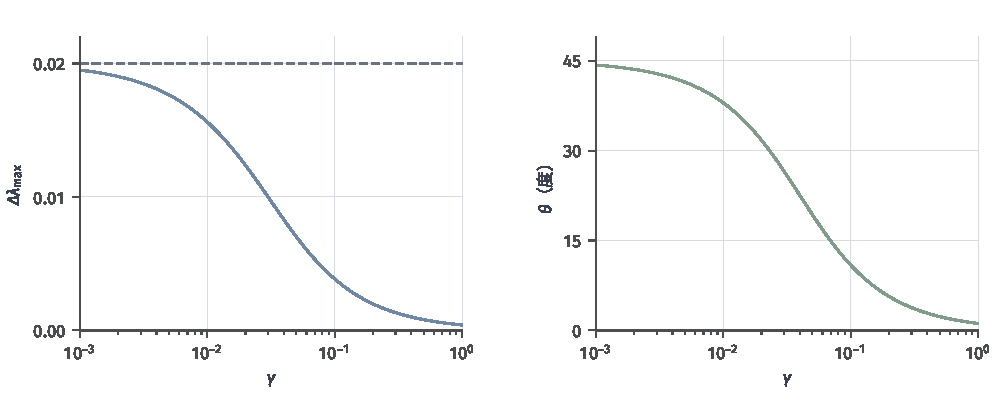
\includegraphics[width=0.92\linewidth]{figures/01-mathematical-preliminaries-upper/03-linear-spaces/matplotlib/matrix-analysis-gap-direction/figure.pdf}
 \caption{谱隙方向示意：$\bm A_\alpha$的两个特征值相距$2\alpha$（谱隙），
 交叉扰动$\varepsilon$把最大特征方向转过约$\varepsilon/(2\alpha)$；
 谱隙越小，同样扰动转过的角度越大。}
 \label{fig:matrix-analysis-gap-direction}
\end{figure}

本节得到的结论是：把矩阵本身当作输入时，对称矩阵的特征值与任意矩阵的奇异值都是良态的，移动不超过$\lVert\bm E\rVert_2$，不要求特征值彼此分开；特征子空间要用与基无关的主夹角比较，它的转角由扰动与谱隙之比控制，谱隙越小越容易被转动；非对称矩阵的特征值可能对扰动非常敏感，敏感程度由特征向量矩阵的条件数或不可对角化的结构决定。条件数与谱的扰动讨论的都是一次作用或一次分解。下一节转向同一个矩阵的反复作用。

% 第6章第8节：矩阵的长期作用（谱半径判据、衰减速度与边界情形、瞬态放大、Neumann级数）。

\section{矩阵的长期作用}
\label{sec:ls-convergence}
\label{sec:linear-algebra-convergence-approximation}
\label{sec:ls-matrix-power-behavior}
\label{sec:linear-algebra-power-convergence}

条件数衡量的是一次作用的放大。迭代法、离散动态系统和许多学习算法却反复施加同一个线性作用，得到序列$\bm x^{(k)}=\bm A^k\bm x^{(0)}$；把这些作用累加起来，又得到矩阵级数。本节回答两个问题。第一，矩阵幂什么时候对所有初值都趋于零，趋近得多快，途中会不会先变大？第二，由矩阵幂组成的级数什么时候收敛，收敛到什么？

讨论收敛时不必担心范数的选择。第~\ref{sec:ls-finite-dimensional-sequences}节已经说明，有限维空间上的任意两个范数彼此等价（定理~\ref{thm:ls-norm-equivalence}），向量或矩阵序列是否收敛与所用范数无关，换范数只改变不等式中的常数。所以下面可以在任意方便的范数下论证，结论对所有范数成立。我们将看到，长期行为由谱半径决定，早期的放大则取决于矩阵是否正规。

\subsection{谱半径判据}

对固定方阵$\bm A$反复作用，初值$\bm x^{(0)}$在第$k$步变成$\bm x^{(k)}=\bm A^k\bm x^{(0)}$。只检查一个初值的轨迹不够：若初值恰好不含某个增长方向的分量，轨迹看起来收敛，换一个初值就发散。下面的反例说明这一点。
\begin{example}[反例：收敛与发散的轨迹]
\label{ex:ls-partial-convergence}
给定$\bm A=\operatorname{diag}(0.5,2)$，比较两个初值的轨迹：
\[
 \bm A^k\begin{bmatrix}1\\0\end{bmatrix}=\begin{bmatrix}0.5^k\\0\end{bmatrix}\to\bm0,\qquad
 \bm A^k\begin{bmatrix}0\\1\end{bmatrix}=\begin{bmatrix}0\\2^k\end{bmatrix},
\]
其中后一条轨迹的长度为$2^k\to\infty$。
结论：初值$(1,0)^\top$不含增长方向$\bm e_2$的分量，轨迹收敛；初值$(0,1)^\top$的轨迹发散。一个初值的轨迹收敛，不能说明矩阵幂趋于零。
\end{example}
所以要问的是：何时对全体初值都有$\bm A^k\bm x^{(0)}\to\bm0$？逐个取$\bm x^{(0)}=\bm e_j$可知，这等价于$\bm A^k$的每一列趋于零，即$\bm A^k\to\bm0$。

图~\ref{fig:ls-spectral-radius-convergence}显示了最简单的正规情形：误差每步乘以$\rho$，$\rho<1$时衰减，$\rho>1$时增长。

\begin{figure*}[htbp]
 \centering
 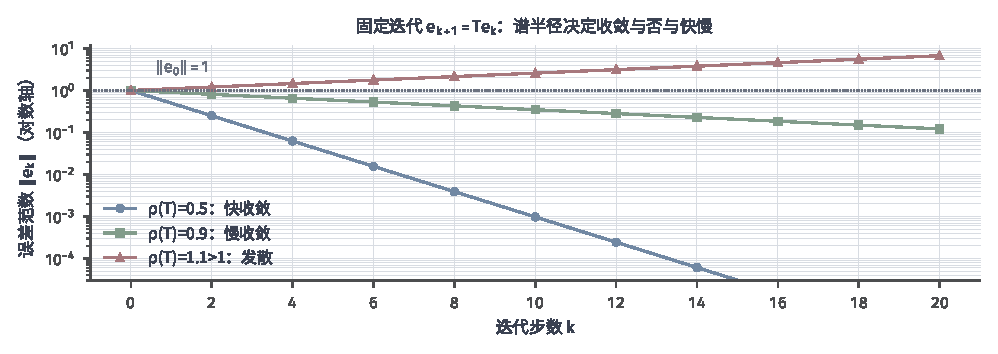
\includegraphics[width=169.0mm]{figures/01-mathematical-preliminaries-upper/03-linear-spaces/matplotlib/ls-spectral-radius-convergence/ls-spectral-radius-convergence.pdf}
 \caption{谱半径决定迭代的长期方向。递推$\bm e^{(t+1)}=\bm A\bm e^{(t)}$、
 $\lVert\bm e^{(0)}\rVert=1$，取正规矩阵$\bm A=\rho\bm I$时$\lVert\bm e^{(t)}\rVert=\rho^t$：
 $\rho=0.5$（蓝）约十四步降到$10^{-4}$，$\rho=0.9$（绿）缓慢下降，
 $\rho=1.1$（红）指数上升。纵轴为半对数。}
 \label{fig:ls-spectral-radius-convergence}
\end{figure*}

最先想到的判据来自范数。由次乘性，$\lVert\bm A^k\rVert\leq\lVert\bm A\rVert^k$，所以只要在某个次乘性矩阵范数下$\lVert\bm A\rVert<1$，就有$\bm A^k\to\bm0$。但这只是充分条件：示例~\ref{ex:ls-nonnormal-norm-radius}的矩阵$\left[\begin{smallmatrix}0.8&4\\0&0.5\end{smallmatrix}\right]$二范数大于$4$，而示例~\ref{ex:ls-triangular-power}已经算出它的幂按$0.8^k$与$0.5^k$趋于零，它的谱半径也只有$0.8$。正规矩阵的范数等于谱半径；非正规矩阵的Schur形中，非对角块以及不呈模长乘旋转形式的$2\times2$对角块都会使范数大于谱半径。下面的引理先用相似变换把每个对角块化为模长乘旋转，再用一次坐标缩放把非对角块压小，从而把谱半径变成一个可用的几何上界。

\begin{lemma}[矩阵幂的几何上界]
\label{lem:ls-power-geometric-bound}
对任意$r>\rho(\bm A)$，存在常数$C_r$，使$\lVert\bm A^k\rVert_2\leq C_rr^k$对所有$k\geq0$成立；等价地，存在一个向量范数，使$\bm A$在它诱导的矩阵范数下不超过$r$。
\end{lemma}
\begin{proof}
取实Schur形$\bm A=\bm Q\bm T\bm Q^\top$，设$\bm T$有$s$个对角块，第$i$块的特征值模长为$|\lambda_i|$。

先处理对角块。每个$2\times2$对角块$\bm T_{i,i}$有一对共轭特征值，按第~\ref{sec:ls-general-square-spectrum}节的论证，在复特征向量的实部、虚部组成的基下，它化为模长乘旋转：$\bm T_{i,i}=\bm P_i(|\lambda_i|\bm R_i)\bm P_i^{-1}$，$\bm R_i$为旋转矩阵；$1\times1$块取$\bm P_i=1$、$\bm R_i=\pm1$。

再压小非对角块。对$0<\varepsilon\leq1$，令分块对角矩阵
\[
 \bm D_\varepsilon=\operatorname{diag}(\varepsilon^{0}\bm P_1,\varepsilon^{1}\bm P_2,\ldots,\varepsilon^{s-1}\bm P_s).
\]
直接相乘，$\bm D_\varepsilon^{-1}\bm T\bm D_\varepsilon$的第$(i,j)$块为$\varepsilon^{j-i}\bm P_i^{-1}\bm T_{i,j}\bm P_j$：对角块是$|\lambda_i|\bm R_i$，二范数不超过$\rho(\bm A)$；$j>i$的块带有因子$\varepsilon^{j-i}\leq\varepsilon$，所以全部非对角块的Frobenius范数不超过$\varepsilon c$，其中$c$与$\varepsilon$无关。把矩阵拆成分块对角部分与非对角部分，得
\[
 \lVert\bm D_\varepsilon^{-1}\bm T\bm D_\varepsilon\rVert_2\leq\rho(\bm A)+\varepsilon c .
\]
取$\varepsilon$足够小，使右端不超过$r$。

最后换回原坐标。令$\bm M=\bm Q\bm D_\varepsilon$，则$\bm A=\bm M(\bm D_\varepsilon^{-1}\bm T\bm D_\varepsilon)\bm M^{-1}$，中间各对$\bm M^{-1}\bm M$相消，$\bm A^k=\bm M(\bm D_\varepsilon^{-1}\bm T\bm D_\varepsilon)^k\bm M^{-1}$，故
\[
 \lVert\bm A^k\rVert_2\leq\lVert\bm M\rVert_2\lVert\bm M^{-1}\rVert_2\,r^k ,
\]
取$C_r=\lVert\bm M\rVert_2\lVert\bm M^{-1}\rVert_2$即可。所求的向量范数取$\bm x\mapsto\lVert\bm M^{-1}\bm x\rVert_2$，它诱导的$\bm A$的范数等于$\lVert\bm M^{-1}\bm A\bm M\rVert_2=\lVert\bm D_\varepsilon^{-1}\bm T\bm D_\varepsilon\rVert_2\leq r$。
\end{proof}

有了这个上界，就能给出矩阵幂衰减的充要条件。
\begin{theorem}[矩阵幂的衰减判据]
\label{thm:ls-power-decay}
对实方阵$\bm A$，$\bm A^k\to\bm0$当且仅当$\rho(\bm A)<1$。
\end{theorem}
\begin{proof}
充分性：取$r$满足$\rho(\bm A)<r<1$，由引理，$\lVert\bm A^k\rVert_2\leq C_rr^k\to0$。必要性：设有特征值$|\lambda|\geq1$。若$\lambda$为实数，其特征向量$\bm v$满足$\lVert\bm A^k\bm v\rVert=|\lambda|^k\lVert\bm v\rVert\not\to0$；若$\lambda$非实，在对应的二维不变子空间中，$\bm A^k$在基$(\bm u,\bm w)$下的矩阵是$|\lambda|^k$乘一个旋转，$\bm A^k\bm u$的坐标长度为$|\lambda|^k\geq1$，不趋于零。两种情形都有$\bm A^k\not\to\bm0$。
\end{proof}

\subsection{衰减速度与边界情形}

判据只回答矩阵幂是否趋于零，同一论证还给出衰减速度。上界$\lVert\bm A^k\rVert\leq C_rr^k$对任意$r>\rho(\bm A)$成立；必要性证明中的特征方向（或不变平面）给出下界$\lVert\bm A^k\rVert\geq c\,\rho(\bm A)^k$，$c>0$为常数。两边开$k$次方，$C_r^{1/k}$与$c^{1/k}$都趋于$1$，于是$\rho(\bm A)\leq\liminf_k\lVert\bm A^k\rVert^{1/k}\leq\limsup_k\lVert\bm A^k\rVert^{1/k}\leq r$。令$r$趋于$\rho(\bm A)$，得到Gelfand公式
\begin{equation}
 \rho(\bm A)=\lim_{k\to\infty}\lVert\bm A^k\rVert^{1/k}.
 \label{eq:ls-gelfand-formula}
\end{equation}
由范数等价（定理~\ref{thm:ls-norm-equivalence}），换成任意矩阵范数只改变常数，开$k$次方后常数的影响消失，所以公式对任意矩阵范数成立。由$\lVert\bm A^k\rVert\leq\lVert\bm A\rVert^k$还得$\rho(\bm A)\leq\lVert\bm A\rVert$对任意次乘性范数成立。

Gelfand公式说明，谱半径是每步放大倍数的长期几何平均：长期看，误差每步大约乘以$\rho(\bm A)$。由$\rho^m=1/10$解出，把误差缩小$10$倍约需$m=1/\log_{10}(1/\rho)$步，$\rho=0.5$时约$3.3$步，$\rho=0.99$时约$229$步；$\rho$越接近$1$，收敛越慢。

$\rho(\bm A)=1$是边界情形，结果取决于模为$1$的特征值。特征值$1$的特征方向保持不动，$-1$的特征方向来回翻转，模为$1$的非实特征值对应纯旋转；在这些方向上$\bm A^k$不趋于零，但保持有界。若模为$1$的特征值缺少足够的特征向量，还会出现增长。
\begin{example}[反例：谱半径为$1$而矩阵幂无界]
\label{ex:ls-unit-spectral-radius-growth}
给定$\bm J_1=\left[\begin{smallmatrix}1&1\\0&1\end{smallmatrix}\right]$，它只有特征值$1$，$\rho(\bm J_1)=1$，特征向量只有$(1,0)^\top$的倍数。按示例~\ref{ex:ls-jordan-block-power}的二项式展开，把$0.8$换成$1$，得
\[
 \bm J_1^k=(\bm I+\bm N)^k=\bm I+k\bm N=\begin{bmatrix}1&k\\0&1\end{bmatrix}.
\]
结论：右上角随$k$线性增长，$\lVert\bm J_1^k\rVert_2\geq k\to\infty$；谱半径等于$1$不能保证矩阵幂有界。
\end{example}
$\rho(\bm A)>1$时，由定理~\ref{thm:ls-power-decay}必要性的证明，从模大于$1$的特征值的特征方向（或不变平面）出发的轨迹不趋于零；但如示例~\ref{ex:ls-partial-convergence}所示，不必每个初值都发散。

\subsection{非正规矩阵的瞬态放大}

$\rho(\bm A)<1$保证最终衰减，但不说明途中的情况。下面的例子中，轨迹先变长、后衰减。
\begin{example}[非正规矩阵的瞬态放大]
\label{ex:ls-transient-growth}
给定迭代
\begin{equation}
 \bm A=\begin{bmatrix}0.8&4\\0&0.5\end{bmatrix},\qquad
 \bm x^{(k+1)}=\bm A\bm x^{(k)},\qquad \bm x^{(0)}=(0,1)^{\top}.
 \label{eq:ch06-fixed-iteration-example}
\end{equation}
示例~\ref{ex:ls-triangular-power}已把初值沿特征向量$\bm v_1=(1,0)^{\top}$、$\bm v_2=(-40/3,1)^{\top}$分解为$\bm x^{(0)}=\tfrac{40}{3}\bm v_1+\bm v_2$，并写出了矩阵幂与轨迹：
\begin{equation}
 \bm A^k=
 \begin{bmatrix}
  0.8^k&\frac{40}{3}(0.8^k-0.5^k)\\
  0&0.5^k
 \end{bmatrix},\qquad
 \bm x^{(k)}=
 \begin{bmatrix}\frac{40}{3}(0.8^k-0.5^k)\\0.5^k\end{bmatrix}.
 \label{eq:ch06-diagonalizable-finite-trajectory}
\end{equation}
代入$k=1,2,3$得
\[
 \bm x^{(1)}=\begin{bmatrix}4\\0.5\end{bmatrix},\qquad
 \bm x^{(2)}=\begin{bmatrix}5.2\\0.25\end{bmatrix},\qquad
 \bm x^{(3)}=\begin{bmatrix}5.16\\0.125\end{bmatrix},
\]
长度分别约为$4.03$、$5.21$、$5.16$，都远大于初值的长度$1$。另一方面$\rho(\bm A)=0.8<1$，由定理~\ref{thm:ls-power-decay}，轨迹最终趋于零。结论：谱半径小于$1$时，轨迹仍可以先放大数倍、再衰减。
\end{example}
放大的原因在于初值的分解。$\tfrac{40}{3}\bm v_1=(40/3,0)^\top$与$\bm v_2=(-40/3,1)^\top$都很长、方向几乎相反，初值$(0,1)^\top$由二者相消而成。两个分量衰减速度不同，相消很快被打破，所以长度先增后降（图~\ref{fig:ch06-transient-growth}）。

\begin{figure*}[htbp]
  \centering
  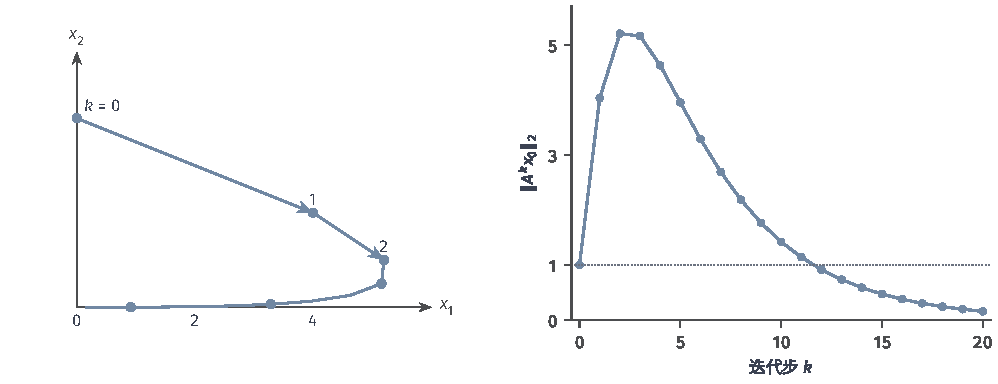
\includegraphics[width=169.0mm]{figures/01-mathematical-preliminaries-upper/03-linear-spaces/matplotlib/ch06-transient-growth/figure.pdf}
  \caption{固定二维矩阵的反复作用。初值为$(0,1)^{\top}$，前两步的长度增加，
  此后回到原点；右图将长度与初始长度$1$比较。特征值$0.8$和$0.5$决定长期衰减，
  非正交特征方向间的相消则决定早期放大。两图使用同一个矩阵和同一组迭代点。}
  \label{fig:ch06-transient-growth}
\end{figure*}

一般地，可对角化矩阵$\bm A=\bm V\bm\Lambda\bm V^{-1}$满足$\bm A^k=\bm V\bm\Lambda^k\bm V^{-1}$，所以
\[
 \lVert\bm A^k\rVert_2\leq\lVert\bm V\rVert_2\lVert\bm V^{-1}\rVert_2\,\rho(\bm A)^k .
\]
特征向量越接近线性相关，$\lVert\bm V\rVert_2\lVert\bm V^{-1}\rVert_2$越大，早期可能的放大越强。正规矩阵则满足$\lVert\bm A^k\rVert_2=\rho(\bm A)^k$（第~\ref{sec:ls-general-square-spectrum}节），不会出现瞬态放大。

不可对角化时，特征向量本身就不够，矩阵幂中还会出现多项式因子。考虑$s$阶矩阵$\bm J=\lambda\bm I+\bm N$，其中$\bm N$是超对角元为$1$、其余元素为零的矩阵，满足$\bm N^s=\bm0$；这样的矩阵称为Jordan块，示例~\ref{ex:ls-jordan-block-power}的$\bm J$是$s=2$的情形。$\lambda\bm I$与$\bm N$可交换，二项式展开成立，且$j\geq s$的项为零：
\begin{equation}
 \bm J^k=\sum_{j=0}^{\min(k,s-1)}\binom{k}{j}\lambda^{k-j}\bm N^j .
 \label{eq:ch06-jordan-power}
\end{equation}
$\binom kj$是$k$的至多$s-1$次多项式，而多项式增长慢于几何衰减，$k^{s-1}|\lambda|^k\to0$（$|\lambda|<1$）。所以$|\lambda|<1$时块幂仍趋于零，只是起初可能上升。下面用二阶块看这种先升后降。
\begin{example}[Jordan块幂的先升后降]
\label{ex:ls-jordan-transient}
给定$\bm J=\left[\begin{smallmatrix}0.8&1\\0&0.8\end{smallmatrix}\right]$与初值$(0,1)^{\top}$。由示例~\ref{ex:ls-jordan-block-power}，
\[
 \bm J^k\begin{bmatrix}0\\1\end{bmatrix}=\begin{bmatrix}k\,0.8^{k-1}\\0.8^k\end{bmatrix}.
\]
第一坐标在$k=1,2,\ldots,6$时依次为$1$、$1.6$、$1.92$、$2.048$、$2.048$、$1.966$（末项保留三位小数），在$k=4,5$时达到最大值约$2.05$，此后才衰减。结论：特征值$0.8<1$保证最终衰减，但多项式因子$k$使第一坐标先上升到初值长度的两倍以上。
\end{example}
图~\ref{fig:vol1-add-linear-jordan-accumulation}画出这条轨迹的两个坐标。多项式因子也是引理~\ref{lem:ls-power-geometric-bound}中常数$C_r$的来源：$r$越接近$\rho(\bm A)$，需要的$\varepsilon$越小，$C_r$可能越大。

\begin{figure}[!htb]
  \centering
  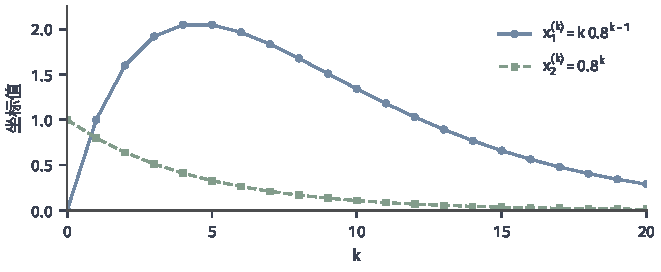
\includegraphics[width=112mm]{figures/01-mathematical-preliminaries-upper/03-linear-spaces/matplotlib/comprehension-additions/linear-jordan-accumulation.pdf}
  \caption{Jordan块的累积项。取正文$\bm J=\left[\begin{smallmatrix}0.8&1\\0&0.8\end{smallmatrix}\right]$与初值$(0,1)^{\top}$。绿线为$0.8^k$，蓝线在$k\geq1$时为$k0.8^{k-1}$，在$k=0$时为$0$。点表示整数步，连线仅引导读图；两坐标最终都趋零。}
  \label{fig:vol1-add-linear-jordan-accumulation}
\end{figure}

所以报告迭代的收敛性时，要分开两件事：谱半径给出长期速度，特征向量的病态程度或Jordan块决定早期可能的放大。

\subsection{Neumann级数}
\label{sec:ls-matrix-series-exponential}

把矩阵幂累加起来会得到什么？最常用的是$\sum_k\bm A^k$，它把求逆$(\bm I-\bm A)^{-1}$写成反复作用之和，也描述每步注入的误差怎样累积。这里说矩阵级数$\sum_{k=0}^{\infty}\bm A^k$收敛，指部分和$\bm S_N=\sum_{k=0}^N\bm A^k$作为矩阵序列收敛。对标量$a$，$|a|<1$时几何级数$\sum_ka^k=1/(1-a)$；矩阵情形有同样的结论。

\begin{theorem}[Neumann级数与逆]
\label{thm:ls-neumann}
若在某个次乘性矩阵范数下$\lVert\bm A\rVert<1$，则级数$\sum_{k=0}^{\infty}\bm A^k$收敛，$\bm I-\bm A$可逆，且
\begin{equation}
 (\bm I-\bm A)^{-1}=\sum_{k=0}^{\infty}\bm A^k,
 \label{eq:ls-neumann-series}
\end{equation}
截断尾项满足$\lVert\sum_{k>N}\bm A^k\rVert\leq\lVert\bm A\rVert^{N+1}/(1-\lVert\bm A\rVert)$。
\end{theorem}
\begin{proof}
由次乘性，$\sum_k\lVert\bm A^k\rVert\leq\sum_k\lVert\bm A\rVert^k<\infty$。由范数等价（定理~\ref{thm:ls-norm-equivalence}），每个元素的绝对值不超过常数乘$\lVert\bm A^k\rVert$，所以每个元素的级数绝对收敛，矩阵级数收敛到某个$\bm S$；尾界由几何级数求和得到。逐项相消，$(\bm I-\bm A)\bm S_N=\bm S_N(\bm I-\bm A)=\bm I-\bm A^{N+1}$，令$N\to\infty$，$\bm A^{N+1}\to\bm0$，得$(\bm I-\bm A)\bm S=\bm S(\bm I-\bm A)=\bm I$。
\end{proof}
条件$\lVert\bm A\rVert<1$可以放宽到谱半径。由引理~\ref{lem:ls-power-geometric-bound}，只要$\rho(\bm A)<1$，就存在使$\lVert\bm A\rVert<1$的诱导范数，所以级数在$\rho(\bm A)<1$时收敛，只是尾界要在那个范数中读取；反之$\rho(\bm A)\geq1$时，由定理~\ref{thm:ls-power-decay}，通项$\bm A^k$不趋于零，级数发散。图~\ref{fig:ls-neumann-series-tail}用一个$2\times2$例子核对尾界。

\begin{figure}[htbp]
 \centering
 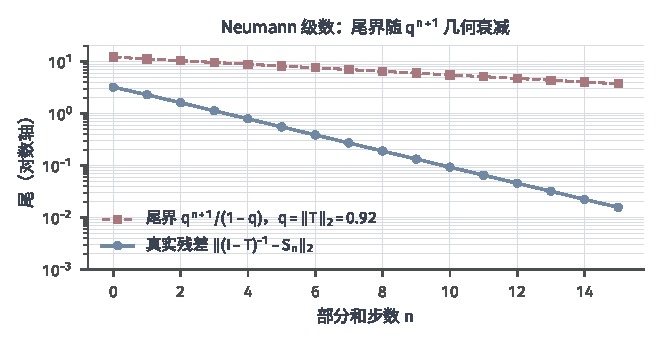
\includegraphics[width=112mm]{figures/01-mathematical-preliminaries-upper/03-linear-spaces/matplotlib/ls-neumann-series-tail/ls-neumann-series-tail.pdf}
 \caption{Neumann级数尾界。$\bm T=[[0.7,0.6],[0,0.1]]$，$q=\lVert\bm T\rVert_2
 \approx0.924<1$，$(\bm I-\bm T)^{-1}=\sum\bm T^k$。蓝线为真实残差
 $\lVert\bm R_n\rVert=\lVert\bm T^{n+1}(\bm I-\bm T)^{-1}\rVert$，红虚线为尾界
 $q^{n+1}/(1-q)$，纵轴半对数（$n=0,\dots,15$）。}
 \label{fig:ls-neumann-series-tail}
\end{figure}

\paragraph{持续扰动的累积}

同样的级数描述持续扰动的累积。迭代的每一步都可能引入新误差（例如舍入），递推成为$\bm e^{(t+1)}=\bm T\bm e^{(t)}+\bm\delta^{(t)}$，$\bm\delta^{(t)}$是第$t$步注入的误差。逐步展开，
\[
 \bm e^{(t)}=\bm T^t\bm e^{(0)}+\sum_{j=0}^{t-1}\bm T^{t-1-j}\bm\delta^{(j)} .
\]
若在某个范数下$\lVert\bm T\rVert\leq q<1$且$\lVert\bm\delta^{(j)}\rVert\leq\delta$，第二项不超过$\delta\sum_{i\geq0}q^i$，于是
\begin{equation}
 \lVert\bm e^{(t)}\rVert\leq q^t\lVert\bm e^{(0)}\rVert+\frac{\delta}{1-q}.
 \label{eq:ls-noise-floor}
\end{equation}
初始误差几何衰减，持续扰动却留下不随$t$下降的误差下限$\delta/(1-q)$；$q$越接近$1$，下限越高。

本节的两个问题至此都有了回答。矩阵幂对全体初值衰减，当且仅当谱半径小于$1$；谱半径还是每步放大倍数的长期几何平均，决定收敛快慢。非正规矩阵在衰减之前可能先放大，放大程度由特征向量的病态程度或不可对角化的结构决定。Neumann级数在谱半径小于$1$时收敛到$(\bm I-\bm A)^{-1}$，持续注入的扰动则留下不随步数下降的误差下限。

% 第6章第9节：本章小结。

\section{本章小结}
\label{sec:ls-analysis-summary}
\label{sec:linear-algebra-summary}
\label{sec:matrix-analysis-summary}

本章围绕一个问题展开：同一个线性作用在什么样的基下最简单，从这个最简形式又能读出它的哪些性质？

前五节逐步调整对基的要求，回答前一半。由特征向量组成的基使矩阵成为对角形；特征值是特征多项式$p_{\bm A}(z)=\det(z\bm I-\bm A)$的根，不随基改变，Cayley--Hamilton定理说明$p_{\bm A}(\bm A)=\bm0$。$n$阶矩阵可对角化，当且仅当它有$n$个线性无关的实特征向量，这时$\bm A^k=\bm V\bm\Lambda^k\bm V^{-1}$。要求基标准正交时，能对角化的恰好是对称矩阵，特征值因而是Rayleigh商的极值；一般方阵只能化为实Schur形，正规矩阵化为分块对角形。输入、输出各取一组标准正交基时，任何矩阵都有奇异值分解，它给出谱范数、Frobenius范数和最佳低秩逼近。

后三节用这些最简形式读出三类性质，它们相互关联而不能互相代替。一次作用的误差放大由条件数$\kappa_2=\sigma_{\max}/\sigma_{\min}$衡量；把矩阵本身当作输入时，对称矩阵的特征值与任意矩阵的奇异值移动不超过$\lVert\bm E\rVert_2$，特征子空间的转角由扰动与谱隙之比控制，非正规矩阵的特征值则可能很敏感；反复作用的长期速度由谱半径决定，$\bm A^k\to\bm0$当且仅当$\rho(\bm A)<1$，但非正规矩阵会先放大再衰减。第~\ref{chap:linear-equations-and-optimization}章求解线性方程、最小二乘与矩阵方程时，将用到奇异值分解、条件数、谱、Cayley--Hamilton定理与实Schur形。


\chapter{线性方程与矩阵方程}
\label{chap:linear-equations-and-optimization}
\label{sec:linear-algebra-reachability-solvability}

前三章建立了研究线性问题的工具：第~\ref{chap:linear-operations}章规定向量与矩阵的运算，
第~\ref{chap:linear-representation}章用列空间、零空间、秩与正交分解描述线性映射的结构，
第~\ref{chap:linear-analysis}章用特征值、奇异值与条件数刻画矩阵作用的强弱方向和误差放大。
这些工具大多从正向计算出发：给定矩阵和输入，按乘法算出输出。实际问题常常反过来，
矩阵和希望得到的输出已经给定，要求找出输入。本章用前面的工具解决三个这样的具体问题。

第一个是线性方程$\bm A\bm x=\bm b$。面对一个具体的方程，先要判断它属于哪种情况：有唯一解、有无穷多解，还是没有解。
有没有解取决于$\bm b$是否落在列空间中，有几个解取决于零空间的大小，二者都可以用秩判别。
三种情况随后分别处理。有唯一解时，问题是怎样高效、稳定地把它算出来，不同结构的矩阵各有适合的分解。
有无穷多解时，要描述全部解，并说明若只报告一个，应当报告哪一个。
没有解时，退而求其次，在所有能产生的输出中找离$\bm b$最近的一个，这就是最小二乘；这个问题又化为一个总有解的线性方程。

三种情况的答案最后由伪逆统一写出。以上讨论都假定数据精确。数据带有误差时，解会偏离多少，要用条件数回答。
小奇异值会使解对误差过于敏感，对此有两类改进：岭回归与截断SVD以改变问题为代价换取稳定；
修正Gram--Schmidt、Householder反射与Givens旋转不改变问题，只让计算本身少引入误差。

第二个是西尔维斯特（Sylvester）方程$\bm A\bm X+\bm X\bm B=\bm C$。它的未知量本身是一张矩阵，左右两侧的乘法同时作用在它上面。
把矩阵拉直成向量后，它又是一个线性方程，但系数矩阵的规模很大。因此我们不形成这个大矩阵，而是直接从$\bm A$、$\bm B$的特征值读出可解条件；
求解时，一般情况下利用它们的实Schur形，可对角化时则换到特征向量坐标直接写出解。

第三个是李雅普诺夫（Lyapunov）方程$\bm A\bm X+\bm X\bm A^\top=\bm Q$，它是Sylvester方程的对称特例。
解的对称性、对称性带来的计算节省以及解的正定性需要单独讨论；与之对应的离散型方程还有一个级数形式的解，正定性可以从中直接读出。

三个方程都按同样的顺序展开：方程表达什么问题，解是否存在、是否唯一，用什么方法求出；
线性方程还要回答求出的解怎样核验，以及数据带误差时解会偏离多少。

% 线性方程Ax=b（上）：问题、解的情况、唯一解的求解方法（分解、例子、比较与核验）、无穷多解（解集与最小范数解）

\section{线性方程}
\label{sec:ls-exact-linear-equations}
\label{sec:linear-algebra-exact-systems}

给定矩阵$\bm A\in\mathbb R^{m\times d}$与目标$\bm b\in\mathbb R^m$，线性方程要求找出输入$\bm x$，
使$\bm A$作用后的输出恰好等于目标：
\begin{equation}
 \bm A\bm x=\bm b,\qquad \bm x\in\mathbb R^d.
 \label{eq:linear-algebra-linear-system}
\end{equation}
它由$m$个方程组成，含$d$个未知量。

若有$s$个目标$\bm b_1,\ldots,\bm b_s$共用同一个矩阵，
可以把它们排成$\bm B\in\mathbb R^{m\times s}$，把未知量排成$\bm X\in\mathbb R^{d\times s}$，
写成$\bm A\bm X=\bm B$。按矩阵乘法逐列读，这就是$s$个方程$\bm A\bm x_j=\bm b_j$并列。
每一列各自有解或无解，互不影响；它们只共享系数矩阵，因而可以共享对$\bm A$所做的计算。

本节按解的情况组织：先用秩判别方程有唯一解、有无穷多解还是没有解，再依次处理这三种情况，
并用伪逆把三种答案统一写出。这些讨论都假定数据精确；最后一部分借助第~\ref{chap:linear-analysis}章的条件数，
分析数据或计算有误差时解会偏离多少，并介绍降低误差影响的几种做法。

\subsection{解的情况}
\label{sec:ls-solution-cases}

按形状，$m=d$的方程称为方阵方程，$m>d$（方程多于未知量）称为超定，$m<d$（方程少于未知量）称为欠定。
一个自然的猜测是：超定方程无解，欠定方程多解，方阵方程恰有一解。下面的两个小方程说明这个猜测不成立。

\begin{example}[反例：形状不决定解的情况]
\label{ex:ls-shape-not-decisive}
超定方程
\[
 \begin{bmatrix}1\\1\end{bmatrix}x=\begin{bmatrix}1\\1\end{bmatrix}
\]
由两个相同的方程$x=1$组成，$x=1$是它的唯一解。方阵方程
\[
 \begin{bmatrix}1&1\\1&1\end{bmatrix}\bm x=\begin{bmatrix}1\\2\end{bmatrix}
\]
由$x_1+x_2=1$与$x_1+x_2=2$组成，两式左边相同而右边不同，互相矛盾，所以无解。
因此超定方程可以有唯一解，方阵方程也可以无解。
\end{example}

形状只限制了秩的上限：秩不超过$\min\{m,d\}$。有没有解要看$\bm b$与$\bm A$的列空间的关系，
有几个解要看$\bm A$的零空间，下面两段分别讨论。这里的“有解”指等式严格成立。
浮点计算中只能比较残差与容限，这一问题留到第~\ref{sec:ls-numerical-sensitivity}节；
算法报告失败，可能只是数值或实现上的问题，不能据此断定方程无解。

\paragraph{有解的条件}
\label{sec:ls-compatibility}

记$\bm a_1,\ldots,\bm a_d$为$\bm A$的各列。按矩阵乘法，$\bm A\bm x=x_1\bm a_1+\cdots+x_d\bm a_d$，
输入只提供组合系数。$\bm x$取遍$\mathbb R^d$时，输出恰好取遍列空间$\operatorname{range}(\bm A)$，所以
\[
 \bm A\bm x=\bm b\ \text{有解}\iff\bm b\in\operatorname{range}(\bm A).
\]
满足这一条件时称方程\term{相容}（consistent）。

为了能具体检验，把$\bm b$并到$\bm A$右侧，得到增广矩阵$[\bm A\;\bm b]$。
若$\bm b$已是原有列的组合，添上它不扩大列张成的空间，秩不变；否则新列带来一个新方向，秩恰好加一。因此
\begin{equation}
 \bm A\bm x=\bm b\ \text{相容}\iff
 \operatorname{rank}[\bm A\;\bm b]=\operatorname{rank}(\bm A).
 \label{eq:ls-augmented-rank}
\end{equation}
用示例~\ref{ex:ls-shape-not-decisive}中的方阵检验这一判据。

\begin{example}[增广矩阵的秩]
\label{ex:ls-augmented-rank-check}
取$\bm A=\left[\begin{smallmatrix}1&1\\1&1\end{smallmatrix}\right]$，它的两列相同，秩为$1$。右端取$\bm b=(1,2)^\top$时，
\[
 [\bm A\;\bm b]=\begin{bmatrix}1&1&1\\1&1&2\end{bmatrix}
\]
含线性无关的两列$(1,1)^\top$与$(1,2)^\top$，秩为$2>1$，所以方程无解，与示例~\ref{ex:ls-shape-not-decisive}的直接观察一致。
右端取$\bm b=(1,1)^\top$时，新列与原有的列相同，$[\bm A\;\bm b]$的秩仍为$1$，所以方程相容。
\end{example}

多右端方程$\bm A\bm X=\bm B$相容，当且仅当每一列$\bm b_j$都在列空间中，
即$\operatorname{rank}[\bm A\;\bm B]=\operatorname{rank}(\bm A)$。这些秩都可以用第~\ref{sec:ls-direct-methods}节的消元法求出。

\paragraph{解的个数}
\label{sec:ls-uniqueness-freedom}

方程相容以后，再问解有几个。若$\bm x_1,\bm x_2$都是解，则$\bm A(\bm x_1-\bm x_2)=\bm0$，两解之差落在零空间
$\operatorname{null}(\bm A)=\{\bm x:\bm A\bm x=\bm0\}$中；反过来，若$\bm x_0$是解且$\bm n\in\operatorname{null}(\bm A)$，
则$\bm A(\bm x_0+\bm n)=\bm b$，$\bm x_0+\bm n$也是解。所以方程相容时，任取一个解$\bm x_0$（称为特解），全部解恰为
\begin{equation}
 \bm x_0+\operatorname{null}(\bm A)=\{\bm x_0+\bm n:\bm n\in\operatorname{null}(\bm A)\}.
 \label{eq:ls-affine-solution-set}
\end{equation}
零空间只含零向量时解唯一；含有非零向量$\bm n$时，$\bm x_0+t\bm n$（$t\in\mathbb R$）已是无穷多个不同的解。
记$r=\operatorname{rank}(\bm A)$，由秩零度定理~\ref{thm:ls-rank-nullity}，$\dim\operatorname{null}(\bm A)=d-r$，
因此相容方程的解唯一，当且仅当$r=d$，即$\bm A$的$d$列线性无关，称为满列秩。

另一种满秩是$r=m$，称为满行秩。此时列空间是整个$\mathbb R^m$，任何右端都相容。
满行秩保证有解，满列秩保证有解时解唯一，下面的例子说明两种保证不能互换。

\begin{example}[反例：满行秩与满列秩互不蕴含]
\label{ex:ls-row-column-rank}
$1\times2$矩阵$\bm A=(1,1)$满行秩：方程$x_1+x_2=b$对每个$b$都有解；但$\bm A(1,-1)^\top=0$，
解可以沿$(1,-1)^\top$任意平移，不唯一。$2\times1$矩阵$\bm A=(1,1)^\top$满列秩：零空间只含零，有解必唯一；
但输出$x(1,1)^\top$的两个分量总相等，只有$\bm b\in\operatorname{span}\{(1,1)^\top\}$时才有解。
\end{example}

据此，超定方程即使满列秩，也只保证“有解则唯一”。欠定方程有$r\leq m<d$，有解时自由参数有$d-r\geq d-m\geq1$个，
所以从不唯一。方阵方程满秩时两种保证同时成立，对每个右端恰有一解，这正是$\bm A$可逆的情形。

\paragraph{方阵的行列式判据}
\phantomsection
\label{sec:ls-determinant-invertibility}
方阵是否可逆还可以由一个数判断。对$n$阶方阵$\bm A$，
\[
 \bm A\text{可逆}\iff\det\bm A\neq0,\qquad
 \bm A^{-1}=\frac{1}{\det\bm A}\operatorname{adj}(\bm A),\qquad
 \det(\bm A^{-1})=\frac{1}{\det\bm A}.
\]

若$\bm A$可逆，由行列式的乘法性（第~\ref{sec:ls-determinant-properties}节），$\det\bm A\det(\bm A^{-1})=\det\bm I_n=1$，
所以$\det\bm A\neq0$，并得第三式。反过来，若$\det\bm A\neq0$，把古典伴随恒等式
$\bm A\operatorname{adj}(\bm A)=\operatorname{adj}(\bm A)\bm A=(\det\bm A)\bm I_n$（定理~\ref{thm:ls-adjugate-identity}）两边除以$\det\bm A$，
就得到一个从左、右两侧乘$\bm A$都给出$\bm I_n$的矩阵，即第二式。二阶时，第二式就是第~\ref{sec:prelim-inverse-matrices}节的二阶求逆公式。

\begin{example}[用伴随矩阵求二阶逆]
\label{ex:ls-adjugate-two-by-two}
取$\bm A=\left[\begin{smallmatrix}2&1\\0&3\end{smallmatrix}\right]$。$\det\bm A=2\cdot3-1\cdot0=6\neq0$，所以$\bm A$可逆。
二阶矩阵的古典伴随由交换两个对角元、两个非对角元变号得到，于是
\[
 \bm A^{-1}=\frac16\begin{bmatrix}3&-1\\0&2\end{bmatrix}.
\]
乘回可验$\bm A\bm A^{-1}=\frac16\left[\begin{smallmatrix}6&0\\0&6\end{smallmatrix}\right]=\bm I_2$，
并且$\det(\bm A^{-1})=\frac1{36}(3\cdot2-0)=\frac16=1/\det\bm A$。
\end{example}

$\det\bm A=0$的几何含义是：单位立方体被$\bm A$压扁成体积为零的形状，列空间不是整个$\mathbb R^n$，有的右端无解。
所以$n$阶方阵方程对每个右端恰有一解，当且仅当$\operatorname{rank}\bm A=n$，也当且仅当$\det\bm A\neq0$。
行列式适合作理论判据，实际判断与求解时并不展开行列式：排列展开有$n!$项，
而第~\ref{sec:ls-direct-methods}节的消元在求解的同时就读出了秩。

\paragraph{三种情况的秩判别}

把两方面合起来，记$\tilde r=\operatorname{rank}[\bm A\;\bm b]$。由于添上一列至多使秩加一，总有$\tilde r=r$或$\tilde r=r+1$，
方程恰属于下面三种情况之一：
\[
 \begin{aligned}
  \tilde r&=r+1: &&\text{无解};\\
  \tilde r&=r=d: &&\text{唯一解};\\
  \tilde r&=r<d: &&\text{无穷多解，全部解含}\ d-r\ \text{个自由参数}.
 \end{aligned}
\]
示例~\ref{ex:ls-augmented-rank-check}的方阵中$r=1<d=2$：
右端$(1,2)^\top$使$\tilde r=2$，属于无解；右端$(1,1)^\top$使$\tilde r=1$，属于无穷多解。
下面三个小节依次处理唯一解、无穷多解与无解。

\subsection{唯一解的求解方法}
\label{sec:ls-direct-methods}
\label{sec:linear-algebra-direct-exact}
\label{sec:matrix-analysis-stable-solvers}

本小节讨论最常见的唯一解情形：$\bm A$是可逆方阵，对每个右端恰有一解。
超定而满列秩的方程在相容时也有唯一解，但判断它是否相容本身就要比较$\bm b$与列空间，
这与最小二乘的计算是同一件事，放到第~\ref{sec:ls-qr-method}节一并处理。

知道解唯一存在，还要把它算出来。三角方程最容易解：上三角方程的最后一个方程只含最后一个未知量，
解出后代入倒数第二个方程，又只剩一个未知量，如此从后向前逐个求出。

本小节的方法都把一般方程化成三角方程，或化成规模更小的方程，在有限步内得到精确算术下的精确解，称为直接法。
它们需要整体读取矩阵并存储分解因子，适合矩阵规模可控、或同一矩阵要配多个右端的情形。

不同方法利用不同的矩阵结构。我们从一般方阵的消元出发，得到LU分解；对称正定矩阵可以省去一半运算，
得到Cholesky分解；对称但不定的矩阵用LDL$^{\top}$分解；具有分块结构或只作低秩修改的矩阵，
可以把大方程化成小方程。用正交变换化三角的QR分解同样能解方程，它与最小二乘一起在第~\ref{sec:ls-qr-method}节讨论。
最后把这些方法的适用条件和代价并列比较，并说明算出的解怎样核验。

\subsubsection{消元与LU分解}

高斯消元用一个方程的倍数去消另一个方程中的未知量。三种行变换——把某行的倍数加到另一行、交换两行、
某行乘非零常数——都可以逆转，因而不改变解集。先看一个二阶的例子。

\begin{example}[二阶方程的消元]
\label{ex:ls-elimination-two-by-two}
解
\[
 \begin{bmatrix}2&1\\4&3\end{bmatrix}\bm x=\begin{bmatrix}1\\3\end{bmatrix},
\]
即$2x_1+x_2=1$、$4x_1+3x_2=3$。第二个方程减去第一个方程的$2$倍，消去$x_1$，得$x_2=1$。
代回第一个方程，$2x_1+1=1$，得$x_1=0$。所以唯一解是$\bm x=(0,1)^\top$。
\end{example}

\paragraph{消元乘子与LU因子}

阶数较高时，消元按列进行，每一步把一列主对角线以下的元素全部消成零。下面的例子显示，
记下每一步所用的倍数，就得到矩阵的一个乘积分解。

\begin{example}[三阶消元与LU分解]
\label{ex:ls-lu-three-by-three}
考虑方程
\[
 \bm A\bm x=\begin{bmatrix}2&1&1\\4&3&3\\8&7&9\end{bmatrix}\bm x
 =\begin{bmatrix}3\\7\\19\end{bmatrix},
\]
先只对系数矩阵$\bm A$消元。第一步以$a_{1,1}=2$为主元，即用来做除数的元素。
第二行减去第一行的$l_{2,1}=4/2=2$倍，变为$(0,1,1)$；第三行减去第一行的$l_{3,1}=8/2=4$倍，变为$(0,3,5)$。
第二步以新的$(2,2)$元$1$为主元，第三行减去第二行的$l_{3,2}=3/1=3$倍，变为$(0,0,2)$。
消元结束时剩下上三角矩阵$\bm U$，三个乘子按位置填进单位下三角矩阵$\bm L$：
\[
 \bm L=\begin{bmatrix}1&0&0\\2&1&0\\4&3&1\end{bmatrix},\qquad
 \bm U=\begin{bmatrix}2&1&1\\0&1&1\\0&0&2\end{bmatrix}.
\]
乘回可验$\bm L\bm U=\bm A$，例如$\bm L\bm U$的第三行是$4\cdot(2,1,1)+3\cdot(0,1,1)+(0,0,2)=(8,7,9)$。
\end{example}

图~\ref{fig:ls-lu-elimination-steps}画出这两步消元，以及乘子怎样按位置收集成$\bm L$。
乘回之所以能复原$\bm A$，是因为消元过程可以倒过来读。$\bm U$的第$i$行，是$\bm A$的第$i$行减去
若干个已经处理好的行（即$\bm U$的前$i-1$行）的倍数得到的，倍数就是乘子$l_{i,k}$：
\[
 \bm U_{i,:}=\bm A_{i,:}-\sum_{k<i}l_{i,k}\bm U_{k,:}
 \quad\Longrightarrow\quad
 \bm A_{i,:}=\sum_{k<i}l_{i,k}\bm U_{k,:}+1\cdot\bm U_{i,:}.
\]
右式说明$\bm A$的第$i$行是$\bm U$各行以$(l_{i,1},\ldots,l_{i,i-1},1,0,\ldots,0)$为系数的组合，
这正是$\bm L\bm U$的第$i$行。因此只要消元中不出现零主元，就有$\bm A=\bm L\bm U$，
其中$\bm L$是对角元为$1$的下三角矩阵，$\bm U$是上三角矩阵，称为LU分解。

有了分解，$\bm A\bm x=\bm b$就是$\bm L(\bm U\bm x)=\bm b$。令$\bm z=\bm U\bm x$，先从前向后解下三角方程
$\bm L\bm z=\bm b$（前代），再从后向前解上三角方程$\bm U\bm x=\bm z$（回代）：
\begin{equation}
 z_i=b_i-\sum_{j<i}l_{i,j}z_j,\qquad
 x_i=\frac{z_i-\sum_{j>i}u_{i,j}x_j}{u_{i,i}}.
\end{equation}
下面用这两个公式完成示例~\ref{ex:ls-lu-three-by-three}的求解。

\begin{example}[用LU因子前代与回代]
\label{ex:ls-lu-forward-back}
沿用示例~\ref{ex:ls-lu-three-by-three}的因子$\bm L,\bm U$与右端$\bm b=(3,7,19)^\top$。前代解$\bm L\bm z=\bm b$：
\[
 z_1=3,\qquad z_2=7-2\cdot3=1,\qquad z_3=19-4\cdot3-3\cdot1=4.
\]
回代解$\bm U\bm x=\bm z$：
\[
 x_3=\frac42=2,\qquad x_2=\frac{1-1\cdot x_3}{1}=-1,
\]
\[
 x_1=\frac{3-1\cdot x_2-1\cdot x_3}{2}=1.
\]
代回原方程，$\bm A(1,-1,2)^\top=(3,7,19)^\top$，所以$\bm x=(1,-1,2)^\top$是方程的解。
\end{example}

前代算出的$\bm z$，正是消元过程对右端做同样变换的结果：例如$z_2=7-2\cdot3$，
就是第二行减去第一行的$2$倍时右端的变化。
\begin{figure}[!htb]
  \centering
  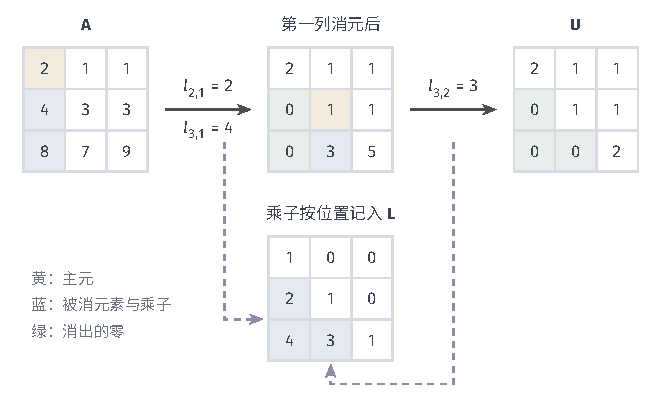
\includegraphics[width=112mm]{figures/01-mathematical-preliminaries-upper/03-linear-spaces/tikz/comprehension-additions/linear-lu-elimination-steps.pdf}
  \caption{三阶矩阵的消元与LU因子。左起依次是$\bm A$、消去第一列后的矩阵与$\bm U$；
  黄色是当前主元，蓝色是待消去的元素，绿色是消出的零。箭头上的乘子等于被消元素除以主元，
  下方按原位置收集成单位下三角因子$\bm L$，满足$\bm L\bm U=\bm A$。}
  \label{fig:ls-lu-elimination-steps}
\end{figure}

\paragraph{选主元}

上面的做法要求每一步的主元不为零。可逆矩阵也可能在主元位置出现零，例如
$\left[\begin{smallmatrix}0&1\\1&1\end{smallmatrix}\right]$的$(1,1)$元为零，无法用它做除数；
交换两行后，以$1$为主元即可继续。主元不为零但很小时，问题同样存在，只是在浮点计算中才暴露出来。
下面的例子用只保留三位有效数字的算术显示这一点。

\begin{example}[小主元与行交换]
\label{ex:ls-partial-pivoting}
解$\left[\begin{smallmatrix}10^{-4}&1\\1&1\end{smallmatrix}\right]\bm x=(1,2)^\top$，
精确解为$x_1=1/(1-10^{-4})\approx1.0001$、$x_2=2-x_1\approx0.9999$。设每步运算结果
只保留三位有效数字（教学设定）。

不交换时，以$10^{-4}$为主元，乘子$l_{2,1}=10^4$。消元后右下角系数
$1-10^4=-9999$舍入为$-1.00\times10^4$，右端$2-10^4=-9998$也舍入为
$-1.00\times10^4$，得$x_2=1.00$，回代$x_1=(1-1.00)/10^{-4}=0$，第一分量完全错误：
大乘子把第二行原有的“$1$”和“$2$”淹没在$10^4$量级中。

先交换两行，以$1$为主元，乘子$l_{2,1}=10^{-4}$。消元后右下角系数$1-10^{-4}$与右端$1-2\times10^{-4}$
都舍入为$1.00$，得$x_2=1.00$，回代$x_1=2-1.00=1.00$，两分量在三位精度下都正确。
两种做法在精确算术中给出同一个解，区别只在乘子大小。
\end{example}

示例~\ref{ex:ls-partial-pivoting}说明，主元比同列其他元素小得多时，乘子会很大，舍入误差随之被放大。
因此第$k$步先在第$k$列尚未处理的元素中选绝对值最大的一个，把它所在的行换到主元位置，再消元。
这种做法称为部分主元，它保证每个乘子满足$|l_{i,k}|\leq1$。把全部行交换累计成置换矩阵$\bm P$，
得到带部分主元的LU分解
\begin{equation}
 \bm P\bm A=\bm L\bm U,
 \label{eq:matrix-analysis-palu}
\end{equation}
求解时先把右端按同样的方式重排，依次解$\bm L\bm z=\bm P\bm b$与$\bm U\bm x=\bm z$。
行交换只改变方程的排列次序，不改变解集。若示例~\ref{ex:ls-lu-three-by-three}也用部分主元，
第一步会把含$8$的第三行换到顶部，得到另一组$\bm P,\bm L,\bm U$，解不变。

行交换不会把奇异矩阵变成可逆矩阵。若某一步在精确算术下，当前列尚未处理的元素全为零，找不到非零主元，
说明这一列是前面主元列的组合，矩阵秩亏。这时跳过该列，继续处理下一列，最后得到阶梯形，非零主元的个数就是秩。

这样，消元同时回答了第~\ref{sec:ls-solution-cases}节的问题。
在阶梯形中，若某行左边全为零而右端非零，即出现$0=c\neq0$的矛盾行，方程不相容，这与增广矩阵的秩判据一致；
若没有矛盾行，把不对应主元的未知量（自由变量）取零，回代即得一个特解，其余解沿零空间展开，
具体做法见第~\ref{sec:ls-select-among-solutions}节。

浮点计算中，一个很小的主元并不能证明矩阵精确奇异：代数上的奇异（主元恰为零）与数值上的接近奇异
（主元很小但非零）是两回事，后者用数值秩描述，见第~\ref{sec:ls-numerical-sensitivity}节。

\paragraph{代价、复用与填充}

稠密$d\times d$矩阵的LU分解约需$2d^3/3$次浮点运算，$\bm L$与$\bm U$可以覆盖原矩阵存放，存储为$O(d^2)$。
分解完成后，每个右端只需前代与回代各一次，运算量为$O(d^2)$。所以同一个$\bm A$配多个右端$\bm b_j$时，
分解只做一次，此后每列只付$O(d^2)$的代价。复用的前提是矩阵不变；矩阵元素一旦改变，旧的$\bm L\bm U$
不再等于新的$\bm P\bm A$，必须重新分解，或改用后文的低秩更新。

稀疏矩阵的情形更微妙。消元会在原来为零的位置产生非零元，称为\term{填充}（fill-in），
使原本稀疏的因子变得接近稠密。填充的多少取决于消元顺序，下面的箭头形矩阵说明这一点。

\begin{example}[箭头形矩阵的填充]
\label{ex:ls-arrow-fill-in}
考虑一个$5\times5$矩阵，其中一个变量与其余全部变量耦合，其余变量彼此不耦合，
非零元只在对角线和这个变量对应的行与列上。

若先消去这个变量，要从其余每一行减去它所在行的倍数，而这一行在所有列上都有非零元，
所以剩下的$4\times4$块全部变成非零：原来只有$4$个对角非零元，现在有$16$个，新增的$12$个都是填充。
若把它排到最后，消去前四个变量时，每一步只改动右下角那一个元素，不产生任何填充。

推广到$n$阶，前一种顺序使因子变为稠密，需存约$n^2$个元素，分解约需$O(n^3)$次运算；
后一种只需原有的$3n-2$个元素和$O(n)$次运算。
\end{example}

图~\ref{fig:ls-sparse-fill-in-ordering}并置了两种顺序。矩阵和解都相同，代价却随顺序相差悬殊，
所以稀疏直接法先选消元顺序、再作分解，其代价也不能只按原始非零元数估计。
\begin{figure}[!htb]
  \centering
  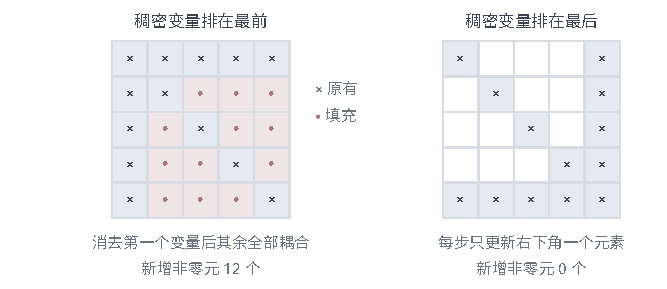
\includegraphics[width=112mm]{figures/01-mathematical-preliminaries-upper/03-linear-spaces/tikz/comprehension-additions/linear-sparse-fill-in-ordering.pdf}
  \caption{消元顺序决定填充。同一个“箭头形”矩阵：左图把与全部变量耦合的变量排在最前，
  消去它后其余位置全部变为非零（红点为填充）；右图把它排在最后，因子保持原有稀疏结构。
  蓝格是原矩阵的非零元。}
  \label{fig:ls-sparse-fill-in-ordering}
\end{figure}

\subsubsection{Cholesky分解}

很多方程的系数矩阵是对称正定的，例如第~\ref{sec:ls-least-squares}节满列秩时的$\bm A^\top\bm A$。
对这类矩阵，LU分解有两处浪费：$\bm U$与$\bm L$实际上携带同样的信息（$\bm U$的第$i$行是$\bm L^\top$的第$i$行乘以第$i$个主元），却要分别计算和存储；
部分主元的行交换会破坏对称性，而对称正定矩阵其实不需要交换。下面说明，对称正定矩阵可以写成
$\bm L\bm L^\top$，只算一个三角因子，并且不必选主元。

设$\bm A=\bm A^\top\succ0$。把第一行、第一列与其余部分分开，也把待求的下三角因子同样分块：
\[
 \bm A=\begin{bmatrix}a_{1,1}&\bm a^\top\\\bm a&\bm A_{22}\end{bmatrix},\qquad
 \bm L=\begin{bmatrix}l_{1,1}&\bm0\\\bm l&\bm L_{22}\end{bmatrix},\qquad
 \bm L\bm L^\top=\begin{bmatrix}l_{1,1}^2&l_{1,1}\bm l^\top\\ l_{1,1}\bm l&\bm l\bm l^\top+\bm L_{22}\bm L_{22}^\top\end{bmatrix}.
\]
令$\bm L\bm L^\top=\bm A$并逐块比较：左上角要求$l_{1,1}^2=a_{1,1}$。正定性给出
$a_{1,1}=\bm e_1^\top\bm A\bm e_1>0$，故可取$l_{1,1}=\sqrt{a_{1,1}}>0$。左下角要求$\bm l=\bm a/l_{1,1}$。
右下角要求
\[
 \bm L_{22}\bm L_{22}^\top=\bm A_{22}-\bm l\bm l^\top=\bm A_{22}-\frac{\bm a\bm a^\top}{a_{1,1}},
\]
问题化为对低一阶的矩阵$\bm A_{22}-\bm a\bm a^\top/a_{1,1}$做同样的分解。

这个剩余矩阵仍然对称正定。对任意非零$\bm u$，取$\bm x=(-\bm a^\top\bm u/a_{1,1},\,\bm u)$，它非零，展开可得
$\bm x^\top\bm A\bm x=\bm u^\top(\bm A_{22}-\bm a\bm a^\top/a_{1,1})\bm u$，而左边为正。
右边正是对第一个变量配方后剩下的二次型。于是同样的论证可以一阶一阶做下去，每一步开方的数都严格为正。
定理~\ref{thm:ls-gram-factor}用同样的配方归纳证明了正定矩阵可写成$\bm L^\top\bm L$的形式，
那里的上三角因子就是这里的$\bm L^\top$；这里把同一构造落实为逐列计算的算法。

\paragraph{Cholesky因子的逐列构造}

总结起来，对称正定矩阵$\bm A$存在唯一的对角元为正的下三角矩阵$\bm L$，使
\begin{equation}
 \bm A=\bm L\bm L^\top,
 \label{eq:matrix-analysis-cholesky}
\end{equation}
称为\term{Cholesky分解}（Cholesky decomposition）。上面的分块递推展开成逐元素的形式，就是按列计算
\begin{equation}
 l_{j,j}=\sqrt{a_{j,j}-\sum_{k<j}l_{j,k}^2},\qquad
 l_{i,j}=\frac{a_{i,j}-\sum_{k<j}l_{i,k}l_{j,k}}{l_{j,j}}\quad(i>j).
\end{equation}
两式都来自比较$\bm L\bm L^\top$与$\bm A$的元素：$\bm L\bm L^\top$的$(i,j)$元（$i\geq j$）是
$\sum_{k\leq j}l_{i,k}l_{j,k}$，其中$k<j$的项只含前面各列，已经算出；剩下的一项$l_{i,j}l_{j,j}$
（$i=j$时是$l_{j,j}^2$）便可解出。根号内的数是第$j$步配方后的剩余，正定性保证它严格为正。
唯一性也由此可见：每个元素都被唯一解出，只有开方有正负两种选择，约定对角元为正就排除了这一任意性。
下面按这两个公式算一个三阶的例子。

\begin{example}[逐列计算Cholesky因子]
\label{ex:ls-cholesky-three-by-three}
取对称矩阵
$\bm A=\left[\begin{smallmatrix}4&2&2\\2&5&3\\2&3&6\end{smallmatrix}\right]$。
第一列：$l_{1,1}=\sqrt4=2$，$l_{2,1}=2/2=1$，$l_{3,1}=2/2=1$。此时剩余矩阵为
\[
 \begin{bmatrix}5&3\\3&6\end{bmatrix}-\begin{bmatrix}1&1\\1&1\end{bmatrix}
 =\begin{bmatrix}4&2\\2&5\end{bmatrix}.
\]
第二列：$l_{2,2}=\sqrt{5-l_{2,1}^2}=\sqrt4=2$，$l_{3,2}=(3-l_{3,1}l_{2,1})/l_{2,2}=(3-1)/2=1$。
第三列：$l_{3,3}=\sqrt{6-l_{3,1}^2-l_{3,2}^2}=\sqrt4=2$。于是
\[
 \bm L=\begin{bmatrix}2&0&0\\1&2&0\\1&1&2\end{bmatrix},
\]
乘回$\bm L\bm L^\top$逐项等于$\bm A$。三个根号内的数都是$4$，都为正。
\end{example}

计算本身也是正定性的检验。若每一步根号内的数都为正，就得到可逆的$\bm L$，
于是对非零$\bm x$有$\bm x^\top\bm A\bm x=\lVert\bm L^\top\bm x\rVert_2^2>0$，$\bm A$正定；
反之，若某一步根号内出现零或负数，$\bm A$就不是正定的。示例~\ref{ex:ls-cholesky-three-by-three}的计算因此同时证明了$\bm A$正定。

求解时，依次解$\bm L\bm z=\bm b$（前代，$z_i=(b_i-\sum_{j<i}l_{i,j}z_j)/l_{i,i}$）与
$\bm L^\top\bm x=\bm z$（回代，$x_i=(z_i-\sum_{j>i}l_{j,i}x_j)/l_{i,i}$）。

\begin{example}[用Cholesky因子求解]
\label{ex:ls-cholesky-solve}
沿用示例~\ref{ex:ls-cholesky-three-by-three}的$\bm A$与$\bm L$，取右端$\bm b=(8,10,11)^\top$。前代解$\bm L\bm z=\bm b$：
\[
 z_1=\frac82=4,\qquad z_2=\frac{10-1\cdot4}{2}=3,\qquad z_3=\frac{11-1\cdot4-1\cdot3}{2}=2.
\]
回代解$\bm L^\top\bm x=\bm z$：
\[
 x_3=\frac22=1,\qquad x_2=\frac{3-1\cdot1}{2}=1,\qquad x_1=\frac{4-1\cdot1-1\cdot1}{2}=1.
\]
代回可验$\bm A(1,1,1)^\top=(8,10,11)^\top$，所以$\bm x=(1,1,1)^\top$。
\end{example}

稠密情形的运算量约为$d^3/3$，是LU的一半；存储也只需一个三角因子，约$d^2/2$个元素。多个右端同样复用一次分解。

矩阵只是半正定时，某一步的配方剩余可能恰为零，后续除以$l_{j,j}$就无法进行。
这时不应随手给对角线加一个小常数让计算通过，那样解的已经是另一个方程。
应先分清原因：$\bm A$本身有零空间时，方程不再有唯一解，回到第~\ref{sec:ls-solution-cases}节判断它属于哪种情况；
剩余量只是因舍入而接近零时，属于数值问题，见第~\ref{sec:ls-numerical-sensitivity}节。
只有任务本身要求加入惩罚项时，才改解相应的正则化方程（第~\ref{sec:ls-regularized-ls}节）。

\subsubsection{LDL$^{\top}$分解}
\label{sec:ls-ldlt}

对称但不定的矩阵，既有使二次型为正的方向，也有使它为负的方向。前面已经说明，逐列计算成功就证明矩阵正定，
所以对不定矩阵，Cholesky的开方必定在某一步遇到非正的数。下面是最小的例子。

\begin{example}[反例：不定矩阵的Cholesky中断]
\label{ex:ls-cholesky-indefinite}
取$\bm A=\left[\begin{smallmatrix}1&2\\2&1\end{smallmatrix}\right]$。它对称，$\det\bm A=-3\neq0$，所以可逆；
但$\bm x=(1,-1)^\top$给出$\bm x^\top\bm A\bm x=1-4+1=-2<0$，$\bm A$不定。按Cholesky的逐列公式，
第一列得$l_{1,1}=1$、$l_{2,1}=2$，第二列要求
\[
 l_{2,2}=\sqrt{a_{2,2}-l_{2,1}^2}=\sqrt{1-2^2}=\sqrt{-3},
\]
在实数中无法进行。
\end{example}

我们仍想利用对称性，只算一个三角因子。办法是不开方，把每一步的主元单独放进对角矩阵$\bm D$，负号就留在$\bm D$里。

\paragraph{LDL$^{\top}$因子的形成}

仍以示例~\ref{ex:ls-cholesky-indefinite}的矩阵为例，看不开方时消元记录下什么。

\begin{example}[二阶不定矩阵的LDL$^{\top}$分解]
\label{ex:ls-ldlt-two-by-two}
对$\bm A=\left[\begin{smallmatrix}1&2\\2&1\end{smallmatrix}\right]$，以$a_{1,1}=1$为主元，乘子$l_{2,1}=2/1=2$，
消元后剩余系数为$1-2\cdot2=-3$。把乘子放进单位下三角矩阵，把两个主元$1$与$-3$放进对角矩阵，得
\[
 \bm A=\begin{bmatrix}1&0\\2&1\end{bmatrix}
 \begin{bmatrix}1&0\\0&-3\end{bmatrix}
 \begin{bmatrix}1&2\\0&1\end{bmatrix}=\bm L\bm D\bm L^\top .
\]
乘回可验等式成立。剩余系数$-3$原样保留在$\bm D$中，不需要开方。
\end{example}

这就是LDL$^{\top}$分解的基本形式：$\bm L$是单位下三角矩阵，$\bm D$是对角矩阵。

只用一阶主元并不总够，下面的矩阵就没有可用的一阶主元。

\begin{example}[反例：没有一阶主元的对称可逆矩阵]
\label{ex:ls-no-scalar-pivot}
取$\bm A=\left[\begin{smallmatrix}0&1\\1&0\end{smallmatrix}\right]$。$\det\bm A=-1\neq0$，所以$\bm A$可逆；
但两个对角元都是零，没有一个能作除数。若像LU那样交换两行，得到的是$\bm P\bm A=\bm L\bm U$形式的分解，
不再是对称的$\bm L\bm D\bm L^\top$。若对称地交换，即同时交换两行和对应的两列，结果仍是$\bm A$本身：
对称置换只重新排列对角元，而这里的对角元全为零。
\end{example}

所以解决办法有两条。一是对称地交换，矩阵仍然对称，对角元被重新排列；若其他位置有合适的对角元，
就可以把它换到主元位置。二是允许用$2\times2$的对称可逆块作主元，在对角元都不合适时必须这样做：
示例~\ref{ex:ls-no-scalar-pivot}的整个矩阵就是一个可逆的二阶块，直接把它放进$\bm D$即可。
一般地，把对称置换累计成$\bm P$，得到
\[
 \bm P\bm A\bm P^\top=\bm L\bm D\bm L^\top,
\]
其中$\bm L$单位下三角，$\bm D$由一阶与二阶对角块组成。

计算过程与LU相同，只是按块进行。把当前待处理的矩阵分块为
$\left[\begin{smallmatrix}\bm A_{11}&\bm A_{21}^\top\\\bm A_{21}&\bm A_{22}\end{smallmatrix}\right]$，
其中$\bm A_{11}$是选定的可逆一阶或二阶主元块。正如标量消元用乘子$l_{i,k}=a_{i,k}/a_{k,k}$，
块消元的乘子块是$\bm L_{21}=\bm A_{21}\bm A_{11}^{-1}$；从下面的块行中减去$\bm L_{21}$乘主元块行，
左下块变成零，右下块变成
\[
 \bm A_{22}-\bm L_{21}\bm A_{21}^\top=\bm A_{22}-\bm A_{21}\bm A_{11}^{-1}\bm A_{21}^\top ,
\]
它仍是对称矩阵，对它重复同样的过程。$\bm L$收集各步的乘子块，$\bm D$收集各步的主元块。
每一步都可以把$\bm L\bm D\bm L^\top$乘回，核对它是否等于置换后的矩阵。

求解时先把右端按$\bm P$重排，再依次解下三角方程$\bm L\bm z=\bm P\bm b$、
块对角方程$\bm D\bm y=\bm z$与上三角方程$\bm L^\top\bm w=\bm y$，最后令$\bm x=\bm P^\top\bm w$还原次序。
其中块对角方程逐块求解：一阶块$d$直接得$y=z/d$；二阶块
$\left[\begin{smallmatrix}d_{11}&d_{12}\\d_{12}&d_{22}\end{smallmatrix}\right]$
的行列式$\Delta=d_{11}d_{22}-d_{12}^2$因主元块可逆而非零，由二阶逆矩阵公式得
\begin{equation}
 y_1=\frac{d_{22}z_1-d_{12}z_2}{\Delta},\qquad
 y_2=\frac{d_{11}z_2-d_{12}z_1}{\Delta}.
\end{equation}
示例~\ref{ex:ls-no-scalar-pivot}的二阶块有$\Delta=-1$，代入得$y_1=z_2$、$y_2=z_1$，
两个未知量一次解出。与Cholesky相比，这一求解过程只是在两次三角求解之间插入了块对角求解，并多了置换与还原；
运算量同样约为$d^3/3$。

最后要分清$\bm D$中的两种情况。负的对角元或不定的二阶块表示矩阵有负方向，但它们可逆，
方程照样唯一可解；零块则表示矩阵奇异，不能当作可逆块做除法，需要回到第~\ref{sec:ls-solution-cases}节重新判断解的情况。

\subsubsection{分块消元与低秩更新}
\label{sec:matrix-analysis-blocks-updates}

LDL$^{\top}$分解中的块消元有更广的用途。若未知量可以自然地分成两组，而且消去其中一组很便宜，
就可以先消去它，只解剩下那组未知量满足的较小方程。先看每组只有一个未知量的最小例子。

\begin{example}[二阶方程的分块消元]
\label{ex:ls-block-elimination-two-by-two}
解$\left[\begin{smallmatrix}2&1\\1&2\end{smallmatrix}\right](x_1,x_2)^\top=(1,3)^\top$。
第一个方程$2x_1+x_2=1$给出$x_1=(1-x_2)/2$。代入第二个方程$x_1+2x_2=3$，得
\[
 \frac{1-x_2}{2}+2x_2=3,\qquad\text{即}\qquad \frac32x_2=3-\frac12=\frac52,
\]
故$x_2=5/3$，回代得$x_1=(1-5/3)/2=-1/3$。核验：$2(-1/3)+5/3=1$，$(-1/3)+2(5/3)=3$。
消去$x_1$后，$x_2$的系数从$2$变成$2-1\cdot\tfrac12\cdot1=\tfrac32$，右端从$3$变成$3-1\cdot\tfrac12\cdot1=\tfrac52$。
\end{example}

图~\ref{fig:ls-schur-block-elimination}把这两步并置。下面把标量换成块，看系数与右端的这两处变化在一般情形下是什么。

\begin{figure*}[htbp]
  \centering
  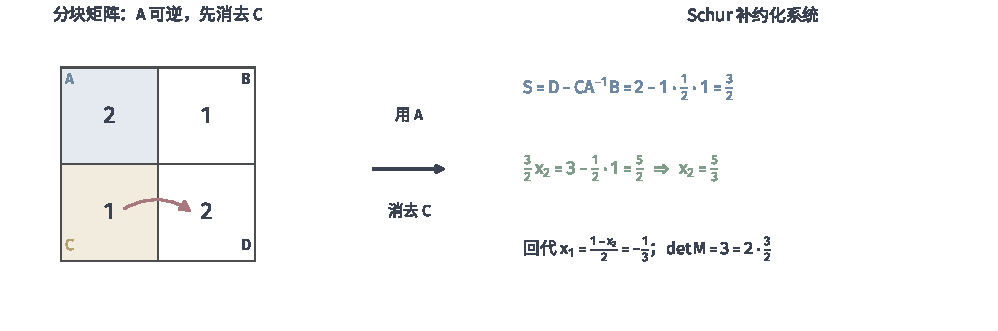
\includegraphics[width=168.998mm]{figures/01-mathematical-preliminaries-upper/03-linear-spaces/matplotlib/ls-schur-block-elimination/ls-schur-block-elimination.pdf}
  \caption{Schur 补的 2×2 分块消元。左：$\bm M=\left[\begin{smallmatrix}2&1\\1&2\end{smallmatrix}\right]$
  按左上块$\bm A=2$分块，先由第一行表出$x_1=(1-x_2)/2$；右：代入第二行后右下角残留
  Schur补$\bm S=3/2$，约化得$x_2=5/3$、回代$x_1=-1/3$，且$\det\bm M=2\cdot3/2=3$。
  解析式教学构造。}
  \label{fig:ls-schur-block-elimination}
\end{figure*}

\paragraph{Schur补与约化系统}

设分块方程为
\[
 \begin{bmatrix}\bm A&\bm B\\\bm C&\bm D\end{bmatrix}
 \begin{bmatrix}\bm x\\\bm y\end{bmatrix}
 =\begin{bmatrix}\bm f\\\bm g\end{bmatrix},
\]
系数矩阵记为$\bm M$，其中$\bm A\in\mathbb R^{p\times p}$可逆。第一组方程$\bm A\bm x+\bm B\bm y=\bm f$
给出$\bm x=\bm A^{-1}(\bm f-\bm B\bm y)$；代入第二组$\bm C\bm x+\bm D\bm y=\bm g$，得
$\bm C\bm A^{-1}\bm f-\bm C\bm A^{-1}\bm B\bm y+\bm D\bm y=\bm g$。整理后，$\bm y$满足
\begin{equation}
 \bm S\bm y=\bm g-\bm C\bm A^{-1}\bm f,
 \qquad
 \bm S=\bm D-\bm C\bm A^{-1}\bm B.
 \label{eq:matrix-analysis-schur-complement}
\end{equation}
矩阵$\bm S$称为$\bm A$在$\bm M$中的\term{Schur补}（Schur complement），方程~\eqref{eq:matrix-analysis-schur-complement}
称为约化系统。
\label{def:matrix-analysis-schur-complement}
示例~\ref{ex:ls-block-elimination-two-by-two}相当于取$\bm A=2$、$\bm B=\bm C=1$、$\bm D=2$、$\bm f=1$、$\bm g=3$，
此时$\bm S=2-1/2=3/2$，约化系统的右端为$3-1/2=5/2$，与那里算出的系数和右端一致。
Cholesky每一步的剩余矩阵$\bm A_{22}-\bm a\bm a^\top/a_{1,1}$，以及LDL$^{\top}$每一步的右下块，都是这样的Schur补。

同一过程写成矩阵乘法，是左乘一个单位块下三角矩阵，消去左下块：
\[
 \begin{bmatrix}\bm I&\bm0\\-\bm C\bm A^{-1}&\bm I\end{bmatrix}
 \begin{bmatrix}\bm A&\bm B\\\bm C&\bm D\end{bmatrix}
 =\begin{bmatrix}\bm A&\bm B\\\bm0&\bm S\end{bmatrix}.
\]
左边第一个因子的行列式为$1$，右边是块上三角矩阵，所以$\det\bm M=\det\bm A\det\bm S$。
因此在$\bm A$可逆的前提下，$\bm M$可逆当且仅当$\bm S$可逆。示例~\ref{ex:ls-block-elimination-two-by-two}中$\det\bm M=3=2\cdot\tfrac32$。

计算时，先解约化系统得到$\bm y$，再回代$\bm x=\bm A^{-1}(\bm f-\bm B\bm y)$。其中凡是出现$\bm A^{-1}$的地方，
都通过对$\bm A$的分解求解来实现，例如$\bm A^{-1}\bm B$由解$\bm A\bm Z=\bm B$得到，不必先形成逆矩阵。
这种做法的典型来源是二部结构：少量全局未知量与大量局部未知量相连，局部未知量彼此之间不直接耦合。
这时$\bm A$是块对角的，消去局部块很便宜，只剩下全局未知量的小系统。

若需要整个逆矩阵，把上述消元过程对一般右端做完，可得块逆公式
\begin{equation}
 \bm M^{-1}=
 \begin{bmatrix}
  \bm A^{-1}+\bm A^{-1}\bm B\bm S^{-1}\bm C\bm A^{-1}
  &-\bm A^{-1}\bm B\bm S^{-1}\\
  -\bm S^{-1}\bm C\bm A^{-1}&\bm S^{-1}
 \end{bmatrix}.
 \label{eq:matrix-analysis-block-inverse}
\end{equation}

$\bm M$对称时$\bm C=\bm B^\top$，Schur补还能判断正定性。对二次型配方：
\begin{equation}
 \begin{bmatrix}\bm x\\\bm y\end{bmatrix}^{\top}
 \bm M\begin{bmatrix}\bm x\\\bm y\end{bmatrix}
 =\bm x^\top\bm A\bm x+2\bm x^\top\bm B\bm y+\bm y^\top\bm D\bm y
 =(\bm x+\bm A^{-1}\bm B\bm y)^\top
 \bm A(\bm x+\bm A^{-1}\bm B\bm y)+\bm y^\top\bm S\bm y,
\end{equation}
展开右边第一项即可验证第二个等号，它多出的$\bm y^\top\bm B^\top\bm A^{-1}\bm B\bm y$正好被$\bm S=\bm D-\bm B^\top\bm A^{-1}\bm B$
中的减项抵消。于是在$\bm A\succ0$时
\begin{equation}
 \bm M\succ0\quad\Longleftrightarrow\quad
 \bm D-\bm B^\top\bm A^{-1}\bm B\succ0.
 \label{eq:matrix-analysis-schur-positive-definite}
\end{equation}
必要性：对任意非零$\bm y$，取$\bm x=-\bm A^{-1}\bm B\bm y$使第一项为零，二次型只剩$\bm y^\top\bm S\bm y$，它必须为正。
充分性：两项都非负；若和为零，则$\bm y^\top\bm S\bm y=0$迫使$\bm y=\bm0$，再由第一项为零得$\bm x=\bm0$。
Cholesky中剩余矩阵保持正定，正是这一结论的特例。

$\bm A$奇异时上述公式不能使用。此时第一组方程$\bm A\bm x=\bm f-\bm B\bm y$本身未必有解，
要求$\bm f-\bm B\bm y$落在$\operatorname{range}(\bm A)$中，至少需要$\operatorname{range}(\bm B)\subseteq\operatorname{range}(\bm A)$
之类的条件，而且$\bm A$的零空间还会给$\bm x$留下自由参数，须按第~\ref{sec:ls-solution-cases}节的判别另行处理。

\paragraph{Woodbury恒等式与小系统}

另一类常见情形是：$\bm A$已经分解好，矩阵却改成了$\bm A+\bm U\bm C\bm V^\top$，其中
$\bm U,\bm V\in\mathbb R^{d\times k}$，$\bm C\in\mathbb R^{k\times k}$，$k$远小于$d$。
例如在最小二乘中增加或删除一条观测，系数矩阵就改变一个秩一项。这里的修改是精确的，不是近似。
重新分解需要$O(d^3)$次运算；能否借旧分解，只解一个$k$阶的小方程？

可以，办法是引入辅助未知量，把问题改写成分块方程，再用上面的Schur补。设$\bm C$可逆，要解
$(\bm A+\bm U\bm C\bm V^\top)\bm x=\bm b$。令$\bm z=\bm C\bm V^\top\bm x\in\mathbb R^k$，原方程等价于
\[
 \bm A\bm x+\bm U\bm z=\bm b,\qquad \bm V^\top\bm x-\bm C^{-1}\bm z=\bm0 .
\]
按约化系统的做法消去$\bm x$：由第一式$\bm x=\bm A^{-1}(\bm b-\bm U\bm z)$，代入第二式得
$\bm V^\top\bm A^{-1}\bm b-\bm V^\top\bm A^{-1}\bm U\bm z-\bm C^{-1}\bm z=\bm0$，即
\[
 (\bm C^{-1}+\bm V^\top\bm A^{-1}\bm U)\bm z=\bm V^\top\bm A^{-1}\bm b .
\]
这是一个$k$阶方程。记它的系数矩阵为$\bm S=\bm C^{-1}+\bm V^\top\bm A^{-1}\bm U$，设其可逆，
则$\bm z=\bm S^{-1}\bm V^\top\bm A^{-1}\bm b$，代回得
$\bm x=\bm A^{-1}\bm b-\bm A^{-1}\bm U\bm S^{-1}\bm V^\top\bm A^{-1}\bm b$。
这对每个$\bm b$都成立，因此得到\term{Woodbury恒等式}
\begin{equation}
 (\bm A+\bm U\bm C\bm V^\top)^{-1}
 =\bm A^{-1}-\bm A^{-1}\bm U
 (\bm C^{-1}+\bm V^\top\bm A^{-1}\bm U)^{-1}
 \bm V^\top\bm A^{-1}.
 \label{eq:matrix-analysis-woodbury}
\end{equation}
使用时同样不形成逆矩阵：用旧分解解出$\bm A^{-1}\bm b$和$\bm A^{-1}\bm U$（共$k+1$个右端，每个右端一次前代、一次回代，代价$O(d^2)$），
形成并求解$k$阶小方程，再组合出$\bm x$，总代价为$O(kd^2+k^3)$。前提是$\bm A$可逆且已有分解，
小矩阵$\bm S$可逆；$\bm S$接近奇异时公式对误差敏感。最常用的是$\bm C=\bm I$，此时只要求
$\bm A$与$\bm I+\bm V^\top\bm A^{-1}\bm U$可逆，对矩形的$\bm U,\bm V$不需要任何逆。

$k=1$时$\bm U=\bm u$、$\bm V=\bm v$是向量，取$\bm C=1$，小方程变成标量方程，得到Sherman--Morrison公式
\[
 (\bm A+\bm u\bm v^\top)^{-1}
 =\bm A^{-1}-\frac{\bm A^{-1}\bm u\bm v^\top\bm A^{-1}}
 {1+\bm v^\top\bm A^{-1}\bm u},
 \qquad 1+\bm v^\top\bm A^{-1}\bm u\neq0 .
\]

行列式也有相应的公式。对上面的分块矩阵
$\left[\begin{smallmatrix}\bm A&\bm U\\\bm V^\top&-\bm C^{-1}\end{smallmatrix}\right]$，
先消左上块，行列式是$\det\bm A\det(-\bm S)$；改为先消右下块$-\bm C^{-1}$，对应的Schur补是
$\bm A-\bm U(-\bm C^{-1})^{-1}\bm V^\top=\bm A+\bm U\bm C\bm V^\top$，行列式是$\det(-\bm C^{-1})\det(\bm A+\bm U\bm C\bm V^\top)$。
两者相等，$k$阶矩阵前的负号各带出$(-1)^k$而抵消，得
$\det(\bm A+\bm U\bm C\bm V^\top)=\det\bm A\det\bm C\det\bm S$。

下面用一个二阶例子核对更新公式与行列式公式。

\begin{example}[秩一更新的求解]
\label{ex:ls-sherman-morrison-update}
取$\bm A=\operatorname{diag}(2,3)$、$\bm u=\bm v=(1,1)^\top$、$\bm b=(1,0)^\top$。
新矩阵是$\bm A+\bm u\bm v^\top=\left[\begin{smallmatrix}3&1\\1&4\end{smallmatrix}\right]$，直接求解得$\bm x=(4/11,-1/11)^\top$。
改用更新公式，只需对旧矩阵$\bm A$求解：
\[
 \bm A^{-1}\bm b=(1/2,\,0)^\top,\qquad
 \bm A^{-1}\bm u=(1/2,\,1/3)^\top,
\]
\[
 1+\bm v^\top\bm A^{-1}\bm u=1+\tfrac12+\tfrac13=\tfrac{11}6,\qquad
 \bm v^\top\bm A^{-1}\bm b=\tfrac12 .
\]
于是小方程的解为$z=(1/2)/(11/6)=3/11$，
\[
 \bm x=\bm A^{-1}\bm b-z\,\bm A^{-1}\bm u
 =\begin{bmatrix}1/2\\0\end{bmatrix}-\frac3{11}\begin{bmatrix}1/2\\1/3\end{bmatrix}
 =\begin{bmatrix}4/11\\-1/11\end{bmatrix},
\]
与直接求解一致。行列式公式给出$\det\bm A\cdot\tfrac{11}6=6\cdot\tfrac{11}6=11$，也与$3\cdot4-1\cdot1=11$一致。
\end{example}

\subsubsection{方法比较与选择}
\label{sec:ls-direct-method-comparison}

上面各方法做的是同一件事：用消元或正交变换把方程化为三角方程或更小的方程。区别在于
各自要求矩阵具备什么结构，以及利用这种结构省下多少运算、存储，稳定性如何。
表~\ref{tab:ls-direct-method-comparison}把这些差别并列，并把第~\ref{sec:ls-qr-method}节的QR一并列入以便比较。
运算量按稠密$d\times d$矩阵（QR按$m\times d$）计；稀疏矩阵的实际代价还取决于消元顺序产生的填充。

\begin{table*}[htbp]
 \centering\small
 \begin{tabularx}{\linewidth}{@{}l>{\raggedright\arraybackslash}X>{\raggedright\arraybackslash}p{24mm}>{\raggedright\arraybackslash}X>{\raggedright\arraybackslash}X>{\raggedright\arraybackslash}X@{}}
  \toprule
  方法 & 适用矩阵 & 稠密运算量 & 存储 & 稳定性 & 典型用途\\
  \midrule
  LU（部分主元） & 一般可逆方阵；秩亏时消元暴露秩与矛盾行 & $2d^3/3$ & $\bm L,\bm U$覆盖原矩阵，另存置换 & 乘子满足$\lvert l_{i,k}\rvert\leq1$，实践中稳定；最坏情形的元素增长极少出现 & 无对称结构的方阵方程；同一矩阵配多个右端\\
  Cholesky & 对称正定 & $d^3/3$ & 一个三角因子，约$d^2/2$个元素 & 不选主元即稳定；根号内出现非正数即说明矩阵不正定 & 满列秩的正规方程、协方差矩阵与核矩阵；也用来检验正定性\\
  LDL$^{\top}$ & 对称不定、可逆 & 约$d^3/3$ & 一个三角因子与块对角$\bm D$ & 需对称选主元（一阶或二阶块）控制乘子；$\bm D$的负块记录负方向 & 等式约束二次优化的最优性方程等鞍点系统\\
  QR & 任意$m\geq d$矩阵，满列秩时回代唯一 & $2md^2-2d^3/3$，方阵约$4d^3/3$ & 反射向量与$\bm R$，约$md$个元素 & 正交变换不放大误差，不形成$\bm A^\top\bm A$ & 超定最小二乘、近秩亏问题（第~\ref{sec:ls-qr-method}节）\\
  分块消元 & 被消去的块可逆，其余块耦合稀疏 & 由被消块的分解与Schur补的阶数决定 & 各块因子与Schur补 & 取决于被消块与Schur补的条件，被消块接近奇异时不可靠 & 二部结构，如三维重建中先消去大量三维点、只解相机参数块\\
  Woodbury & 已分解矩阵加秩$k$修改，$k\ll d$ & 已有因子时$O(kd^2+k^3)$ & 旧因子、修改因子与$k$阶小矩阵 & 小系统接近奇异时敏感 & 增删一条观测后更新解（$k=1$即Sherman--Morrison）\\
  \bottomrule
 \end{tabularx}
 \caption{线性方程直接解法的比较。从上到下，前三种按对称性与正定性逐步收窄适用范围、
 换取更低的运算与存储；QR以更高运算量换取不形成$\bm A^\top\bm A$；后两种不是独立分解，
 而是借已有求解器把大系统化为小系统。}
 \label{tab:ls-direct-method-comparison}
\end{table*}

选择方法时，按结构由特殊到一般逐项检查，越特殊的结构能省下越多代价。

第一，看是否已有分解、矩阵只作了低秩修改，或者矩阵有可以先消去的分块结构。
例如矩阵形如$\bm G=\sum_i\bm a_i\bm a_i^\top$时（第~\ref{sec:ls-least-squares}节的正规方程就是这种形式），
每新增一条观测$\bm a$，$\bm G$只增加一个秩一项$\bm a\bm a^\top$，用Sherman--Morrison借旧分解更新解只需$O(d^2)$，
重新分解则需$O(d^3)$。

第二，看对称性与正定性。上面的$\bm G$在各$\bm a_i$张成全空间时对称正定，用Cholesky最省。
对称而不定的矩阵则不能用Cholesky。

一个典型的对称不定矩阵来自带等式约束的二次优化。在正定二次目标上加等式约束，
其最优性条件（第~\ref{chap:optimization}章的KKT条件）是以
$\left[\begin{smallmatrix}\bm H&\bm C^\top\\\bm C&\bm0\end{smallmatrix}\right]$
为系数矩阵的线性方程，其中$\bm H\succ0$、$\bm C\neq\bm0$。这个矩阵对称，取$\bm y=\bm0$、$\bm x\neq\bm0$可得正方向，
但它也必有负方向：取$\bm y$使$\bm C^\top\bm y\neq\bm0$，再取$\bm x=-\bm H^{-1}\bm C^\top\bm y$，
代入前面的配方公式（其中$\bm A=\bm H$、$\bm B=\bm C^\top$、$\bm D=\bm0$），第一项为零，第二项是
$\bm y^\top(\bm0-\bm C\bm H^{-1}\bm C^\top)\bm y=-(\bm C^\top\bm y)^\top\bm H^{-1}(\bm C^\top\bm y)<0$。
所以它要用LDL$^{\top}$或LU。

第三，没有对称结构时，用部分主元LU。最后，若问题本身是超定的最小二乘，或列之间接近线性相关，
用QR比先形成正规方程更可靠。无论选哪一种，都要先核对前提：把不定矩阵交给Cholesky，
会在某一步遇到非正的配方剩余而中断；把奇异的被消块交给分块消元，约化系统根本无法形成。

\subsubsection{结果核验}
\label{sec:ls-linear-equation-verification}

算出$\bm x$后还要确认它确实满足原方程。三角方程或约化系统解对了，不等于原方程成立：
置换是否还原、乘子是否记错、小系统的解是否正确回代，都只能回到原方程检查。
具体做法是计算残差$\bm r=\bm b-\bm A\bm x$，报告$\lVert\bm r\rVert$或相对残差
$\lVert\bm r\rVert/\lVert\bm b\rVert$（$\bm b\neq\bm0$时），与任务给定的容限比较；多右端时逐列计算，
不能用一列的残差代替另一列。以示例~\ref{ex:ls-elimination-two-by-two}为例，解出$\bm x=(0,1)^\top$，
代回得$\bm A\bm x=(1,3)^\top$，残差为零。

所用方法的前提也要复核：Cholesky要求对称正定，LDL$^{\top}$要求所选主元块可逆，分块消元要求被消去的块可逆。
若计算中途发现矩阵奇异，结论就不再是“解唯一”，应按第~\ref{sec:ls-solution-cases}节给出可复核的依据：
无解时给出消元中出现的矛盾行，多解时给出一个特解和零空间的一组基。

最后，残差小只说明$\bm x$几乎满足方程，不说明$\bm x$离真解近。矩阵接近奇异时，
很小的残差可能对应很大的解误差。第~\ref{chap:linear-analysis}章的条件数正是误差与残差之间的放大倍数，
它对线性方程的具体含义见第~\ref{sec:ls-numerical-sensitivity}节。

\subsection{无穷多解}
\label{sec:ls-select-among-solutions}

秩亏而相容时，即$\operatorname{rank}[\bm A\;\bm b]=\operatorname{rank}(\bm A)=r<d$，方程有无穷多解。
这时要做两件事：先把全部解描述清楚，并算出描述所需的特解与零空间的基；
再说明若只报告一个答案，应当报告哪一个，以及怎样计算它。

\subsubsection{解集的结构}
\label{sec:linear-algebra-affine-relations}

第~\ref{sec:ls-uniqueness-freedom}节已经证明，全部解是$\bm x_0+\operatorname{null}(\bm A)$，
即把子空间$\operatorname{null}(\bm A)$平移到某个特解$\bm x_0$处得到的集合。这样的集合称为\term{仿射空间}（affine space）。
基点$\bm x_0$可以换成任何别的解，集合本身不变；方向空间$\operatorname{null}(\bm A)$则由集合唯一确定，
因为它恰好由集合中任意两点之差组成。例如$x_1+x_2=2$有特解$(1,1)^\top$，
零空间由$(1,-1)^\top$张成，全部解为$(1,1)^\top+t(1,-1)^\top$，$t\in\mathbb R$。

换个角度看，按“输出是否相同”把输入分组，同一组中任意两点之差都在零空间中，每组正是零空间的一个平移。
方程$\bm A\bm x=\bm b$的解集，就是输出为$\bm b$的那一组。
图~\ref{fig:vol1-add-linear-nullspace-fibers}以$\bm A=(1,1)$画出这种分组：
每条平行线$x_1+x_2=c$上的点产生同一个输出$c$。
\begin{figure}[!htb]
  \centering
  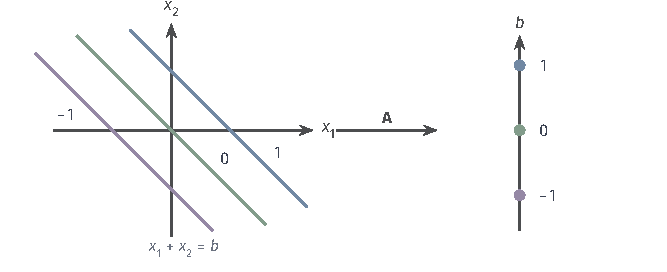
\includegraphics[width=112mm]{figures/01-mathematical-preliminaries-upper/03-linear-spaces/tikz/comprehension-additions/linear-nullspace-fibers.pdf}
  \caption{同一输出对应的整组输入。对$\bm A=(1,1)$，蓝、绿、紫直线分别满足
  $x_1+x_2=1,0,-1$；右侧同色点是各直线的输出。绿色直线是$\ker\bm A$，
  其余直线是它的平移。把一整条直线归为一类后，才得到与可达输出的一一对应。}
  \label{fig:vol1-add-linear-nullspace-fibers}
\end{figure}

解集有多大，由零空间的维数决定。$\dim\operatorname{null}(\bm A)=d-r$，取零空间的一组基$\bm n_1,\ldots,\bm n_{d-r}$，
全部解可写成$\bm x_0+t_1\bm n_1+\cdots+t_{d-r}\bm n_{d-r}$，其中$t_1,\ldots,t_{d-r}$任意取值，
所以解集有$d-r$个自由参数。上例中$d=2$、$r=1$，自由参数只有$t$一个。

\paragraph{特解与零空间基的计算}

这一描述需要两样东西：一个特解和零空间的一组基。二者都可以从消元得到的阶梯形读出
（第~\ref{sec:ls-direct-methods}节）。主元所在的列对应主元变量，其余未知量称为自由变量，共$d-r$个。
把全部自由变量取零，回代解出主元变量，就得到一个特解；把右端换成零，令某一个自由变量取$1$、其余取零，
回代得到零空间中的一个向量，依次对每个自由变量这样做，得到的$d-r$个向量线性无关，构成零空间的一组基。
下面的例子按这一步骤计算。

\begin{example}[从阶梯形读出特解与零空间的基]
\label{ex:ls-particular-null-basis}
解
\[
 \begin{bmatrix}1&2&1\\2&4&3\end{bmatrix}\bm x=\begin{bmatrix}4\\9\end{bmatrix}.
\]
第二行减去第一行的$2$倍，得阶梯形
\[
 \begin{bmatrix}1&2&1\\0&0&1\end{bmatrix}\bm x=\begin{bmatrix}4\\1\end{bmatrix},
\]
即$x_3=1$。主元在第一、三列，$x_2$是自由变量，$r=2$、$d-r=1$。取$x_2=0$，
回代$x_1=4-2x_2-x_3=3$，得特解$\bm x_0=(3,0,1)^\top$。右端换成零并取$x_2=1$，得$x_3=0$、$x_1=-2$，
零空间由$\bm n=(-2,1,0)^\top$张成。所以全部解为
\[
 \bm x=(3-2t,\,t,\,1)^\top,\qquad t\in\mathbb R .
\]
代回可验$\bm A\bm x_0=(4,9)^\top$、$\bm A\bm n=\bm0$。
\end{example}

\subsubsection{最小范数解}

方程本身给出的是整个仿射空间$\bm x_0+\operatorname{null}(\bm A)$，并不指定其中哪一个点。
若要报告一个确定的答案，必须另加准则。
最常用的准则是取欧氏范数最小的解，几何上就是在仿射空间中找离原点最近的点。

准则需要事先声明，因为不同准则选出的点不同：换一个内积，离原点“最近”的点一般也会改变。
示例~\ref{ex:ls-particular-null-basis}的特解$(3,0,1)^\top$也是一个合法的解，
只是它来自“自由变量取零”这一约定，换一种消元顺序就会得到另一个特解。

为求范数最小的点，把输入分成两部分：被$\bm A$消去的部分和真正决定输出的部分。
第一部分属于$\operatorname{null}(\bm A)$；第二部分应取在它的正交补中。
由定理~\ref{thm:ls-four-subspaces-orthogonality}，这个正交补就是行空间，$\operatorname{null}(\bm A)^\perp=\operatorname{range}(\bm A^\top)$，
输入空间有正交直和$\mathbb R^d=\operatorname{range}(\bm A^\top)\oplus\operatorname{null}(\bm A)$（式~\eqref{eq:ls-four-subspaces-decomposition}）：
$\operatorname{null}(\bm A)$是被消去的输入方向，$\operatorname{range}(\bm A^\top)$是真正影响输出的方向。

\paragraph{最小范数精确解的唯一性}

按输入空间的分解，每个解唯一写成$\bm x=\bm x_R+\bm x_N$，其中$\bm x_R\in\operatorname{range}(\bm A^\top)$，
$\bm x_N\in\operatorname{null}(\bm A)$。所有解共有同一个$\bm x_R$：若$\bm x'=\bm x'_R+\bm x'_N$是另一个解，
则$\bm x_R-\bm x'_R=(\bm x-\bm x')-(\bm x_N-\bm x'_N)$既在$\operatorname{range}(\bm A^\top)$中，
又是两个零空间向量之差，落在$\operatorname{null}(\bm A)$中；两个子空间互相正交，只交于零向量，故$\bm x_R=\bm x'_R$。
由于$\bm A\bm x_N=\bm0$，$\bm A\bm x_R=\bm A\bm x=\bm b$，$\bm x_R$本身也是解。两部分正交，勾股恒等式给出
\[
 \lVert\bm x\rVert_2^2=\lVert\bm x_R\rVert_2^2+\lVert\bm x_N\rVert_2^2\geq\lVert\bm x_R\rVert_2^2,
\]
等号当且仅当$\bm x_N=\bm0$。所以最小范数解存在且唯一，就是解集中落在$\operatorname{range}(\bm A^\top)$里的那一个。
用前面的直线方程核对这一刻画。

\begin{example}[直线$x_1+x_2=2$上的最小范数解]
\label{ex:ls-min-norm-line}
方程$x_1+x_2=2$的系数矩阵为$\bm A=(1,1)$，全部解为$(1+t,1-t)^\top$，$t\in\mathbb R$。它们的范数平方为
\[
 (1+t)^2+(1-t)^2=2+2t^2,
\]
在$t=0$时最小，所以最小范数解是$(1,1)^\top$。它正比于$\bm A^\top=(1,1)^\top$，确实落在$\operatorname{range}(\bm A^\top)$中。
\end{example}

\paragraph{最小范数解的计算}

这一刻画也给出计算方法。设$\bm A$满行秩，要找的解形如$\bm x=\bm A^\top\bm w$，代入方程得
$\bm A\bm A^\top\bm w=\bm b$。$m$阶方阵$\bm A\bm A^\top$可逆：若$\bm A\bm A^\top\bm w=\bm0$，
则$\lVert\bm A^\top\bm w\rVert_2^2=\bm w^\top\bm A\bm A^\top\bm w=0$，即$\bm A^\top\bm w=\bm0$，
而$\bm A^\top$的$m$列线性无关，迫使$\bm w=\bm0$。于是最小范数解为
\[
 \bm x=\bm A^\top(\bm A\bm A^\top)^{-1}\bm b .
\]
实际计算时不形成逆矩阵：$\bm A\bm A^\top$对称正定，先用Cholesky分解解出$\bm w$，再算$\bm A^\top\bm w$。

\begin{example}[满行秩方程的最小范数解]
\label{ex:ls-min-norm-row-full-rank}
示例~\ref{ex:ls-particular-null-basis}的系数矩阵$\bm A=\left[\begin{smallmatrix}1&2&1\\2&4&3\end{smallmatrix}\right]$的秩为$2$，满行秩。计算
\[
 \bm A\bm A^\top=\begin{bmatrix}6&13\\13&29\end{bmatrix},
\]
解$\bm A\bm A^\top\bm w=(4,9)^\top$得$\bm w=(-1/5,2/5)^\top$，于是
\[
 \bm x=\bm A^\top\bm w=(3/5,\,6/5,\,1)^\top .
\]
它是全部解$(3-2t,t,1)^\top$中$t=6/5$的那一个，与零空间方向$(-2,1,0)^\top$正交。
它的范数平方为$14/5$，小于特解$(3,0,1)^\top$的范数平方$10$。
\end{example}

矩阵$\bm A^\top(\bm A\bm A^\top)^{-1}$从右边乘$\bm A$得到单位矩阵，是第~\ref{sec:prelim-inverse-matrices}节介绍过的右逆中的一个。
右逆不唯一，其他右逆给出的一般不是最小范数解。

\begin{example}[反例：其他右逆不给出最小范数解]
\label{ex:ls-other-right-inverse}
取$\bm A=(1,1)$。右逆$\bm A^\top(\bm A\bm A^\top)^{-1}=(1/2,1/2)^\top$把$b$送到最小范数解$(b/2,b/2)^\top$，范数为$|b|/\sqrt2$。
$(1,0)^\top$也满足$\bm A(1,0)^\top=1$，是另一个右逆；它把$b$送到$(b,0)^\top$。这也是方程的解，
但范数为$|b|$，$b\neq0$时大于最小范数。
\end{example}

形成$\bm A\bm A^\top$会把各行之间接近线性相关的程度放大（第~\ref{sec:ls-normal-equations-method}节对$\bm A^\top\bm A$说明了同样的现象）。
更可靠的做法是对$\bm A^\top$作第~\ref{chap:linear-representation}章的经济型QR分解~\eqref{eq:ls-qr-factorization}，
$\bm A^\top=\bm Q\bm R$，$\bm Q$是$d\times m$矩阵，$\bm R$是$m$阶可逆上三角矩阵。
最小范数解落在$\operatorname{range}(\bm A^\top)=\operatorname{range}(\bm Q)$中，可写成$\bm x=\bm Q\bm w$。
代入方程，$\bm A\bm x=\bm R^\top\bm Q^\top\bm Q\bm w=\bm R^\top\bm w=\bm b$，
这是下三角方程，前代即得$\bm w$。所得的解与上面的公式相同，但不形成$\bm A\bm A^\top$；
QR分解怎样稳定地计算，见第~\ref{sec:ls-orthogonalization-qr}节。

$\bm A$不满行秩时，有些方程可以由其他方程组合出来，$\bm A\bm A^\top$不可逆，上面的公式不能直接使用。
方程相容时，可以先删去这些多余的方程，化为满行秩的情形；要把最小范数解写成一个矩阵作用于$\bm b$，
则需要第~\ref{sec:ls-pseudoinverse}节的伪逆。

至此，无穷多解的情形已经回答：全部解是一个特解加零空间，二者都可由消元读出；
若只报告一个解，须声明准则，欧氏范数最小的解是解集中唯一落在$\operatorname{range}(\bm A^\top)$里的点，
满行秩时可由$\bm A\bm A^\top$的Cholesky分解或$\bm A^\top$的QR分解算出。

% 线性方程Ax=b（下）：无解时的最小二乘（问题与正规方程、解的性质、求解方法、投影矩阵、核验）、
% 伪逆（构造、统一三种情况、Penrose条件）、数值敏感性（方程解、残差与后向误差、最小二乘、数据计算优化：
% 岭回归、修正Gram--Schmidt、截断SVD、Householder反射、Givens旋转）

\subsection{无解：最小二乘}
\label{sec:ls-least-squares}
\label{sec:linear-algebra-residual-systems}
\label{sec:linear-algebra-projection-least-squares}
\label{sec:matrix-analysis-inverse-input-selection}

剩下的情况是$\operatorname{rank}[\bm A\;\bm b]>\operatorname{rank}(\bm A)$：$\bm b$不在列空间中，方程$\bm A\bm x=\bm b$无解。
这在实际中很常见：观测带有误差，方程数又往往多于未知量，几乎不可能被某个输入精确产生。
这时不再寻找不存在的精确解，而是在全部可达输出$\operatorname{range}(\bm A)$中找离$\bm b$最近的一个，再求产生它的输入。
本小节先把这个问题写成一个线性方程，然后对它回答前面的同一组问题：解是否存在、是否唯一，怎样计算，怎样核验。

\subsubsection{问题与正规方程}
\label{sec:ls-ordinary-ls}
\label{sec:ls-least-squares-objective}
\label{sec:ls-subspace-nearest-points}
\label{sec:linear-algebra-decomposition-projection}

给定$\bm A\in\mathbb R^{m\times d}$和观测$\bm b\in\mathbb R^m$，改求使输出误差的平方长度最小的输入：
\begin{equation}
 \min_{\bm x\in\mathbb R^d}\ \lVert\bm A\bm x-\bm b\rVert_2^2.
 \label{eq:linear-algebra-least-squares}
\end{equation}
这一问题称为\term{最小二乘}（least squares）。回归中常写成$\bm X\bm w\approx\bm y$，
设计矩阵$\bm X$对应$\bm A$，系数$\bm w$对应$\bm x$，响应$\bm y$对应$\bm b$，是同一个问题。
用长度的平方而不用长度本身，最小点不变，但目标成为$\bm x$的二次函数，后面的推导由此得以化成线性方程。
若$\bm b\in\operatorname{range}(\bm A)$，最小值为零，最小点就是相容方程的解；精确求解是最小二乘的特殊情形。

观测也可以有若干列。给定$\bm B\in\mathbb R^{m\times n}$，求$\bm X\in\mathbb R^{d\times n}$使
\begin{equation}
 \min_{\bm X}\ \lVert\bm A\bm X-\bm B\rVert_{\mathrm F}^2
 =\sum_{j=1}^n\lVert\bm A\bm x_j-\bm b_j\rVert_2^2,
 \label{eq:ls-multi-right-frobenius}
\end{equation}
其中$\bm b_j$、$\bm x_j$分别是$\bm B$、$\bm X$的第$j$列。Frobenius范数的平方把各列残差的平方长度相加，
第$j$项只含$\bm x_j$，各项可以分别取最小。因此多右端问题就是$n$个共用矩阵的最小二乘问题并列，
下面只讨论单列，对$\bm A$所做的分解可以复用于全部列。

\paragraph{子空间最近点}

目标$\lVert\bm A\bm x-\bm b\rVert_2^2$只通过拟合值$\bm A\bm x$依赖输入，而拟合值取遍列空间。
所以问题可以分两步：先在列空间中找离$\bm b$最近的点，再求产生这个点的输入。
第一步只涉及一个子空间和一个目标，我们在一般的有限维实内积空间中讨论它，结论对加权内积和函数空间也适用。

设$V$为有限维实内积空间，$U\subseteq V$为子空间，给定目标$\bm y\in V$。
\term{子空间最近点}问题要求找出$\bm p\in U$，使距离$\lVert\bm y-\bm p\rVert$最小。
距离由内积诱导，换一个内积，“最近”的含义也随之改变。
第~\ref{sec:ls-select-among-solutions}节在解集中挑选范数最小的解，也是这种问题：在一个平移的子空间中找离原点最近的点。

取$U$的一组基$\bm b_1,\ldots,\bm b_r$，排成基矩阵$\bm B=[\bm b_1\;\cdots\;\bm b_r]$（与上面的多右端观测矩阵无关），
则$U=\{\bm B\bm c:\bm c\in\mathbb R^r\}$，最近点问题化为求系数
\begin{equation}
 \min_{\bm c\in\mathbb R^r}\lVert\bm y-\bm B\bm c\rVert_2.
 \label{eq:ls-nearest-point-coefficients}
\end{equation}
它正是以$\bm B$为系数矩阵的最小二乘问题。换一组基只改变系数$\bm c$，不改变点集$U$，因而不改变最近点。

困难在于基向量一般互不正交，系数不能由逐个内积直接读出。

\begin{example}[反例：非正交基下系数不等于内积]
\label{ex:ls-nonorthogonal-coefficients}
在$\mathbb R^2$中取基$\bm b_1=(1,1)^\top$、$\bm b_2=(1,0)^\top$和目标$\bm y=(0,1)^\top$。
$\bm y$与两个基向量的内积分别是$\langle\bm b_1,\bm y\rangle=1$与$\langle\bm b_2,\bm y\rangle=0$。
但$\bm y=\bm b_1-\bm b_2$，真正的系数是$1$和$-1$，第二个系数与内积$0$不符。
\end{example}

所以下面先不借助基，从几何上刻画最近点，再把刻画翻译成系数满足的方程。

\paragraph{正交性判据}

由第~\ref{sec:ls-orthogonality}节的正交直和（引理~\ref{lem:ls-orthogonal-decomposition}），
$\bm y$可以唯一写成$\bm y=\bm p+\bm r$，其中$\bm p\in U$，$\bm r\in U^\perp$。我们证明这个$\bm p$就是最近点。
对任意$\bm u\in U$，把$\bm y-\bm u$拆成$(\bm p-\bm u)+\bm r$：第一项在$U$中，第二项在$U^\perp$中，二者正交，
勾股恒等式给出
\begin{equation}
 \lVert\bm y-\bm u\rVert_2^2
 =\lVert\bm p-\bm u\rVert_2^2+\lVert\bm r\rVert_2^2
 \geq\lVert\bm r\rVert_2^2,
 \label{eq:ls-nearest-point-pythagoras}
\end{equation}
等号当且仅当$\bm u=\bm p$。因此最近点存在且唯一，最小距离为$\lVert\bm r\rVert_2$，
残差$\bm r=\bm y-\bm p$与$U$正交。

反过来，若某个$\bm p\in U$使$\bm y-\bm p\perp U$，同样的拆分$\bm y-\bm u=(\bm p-\bm u)+(\bm y-\bm p)$
仍是正交的，于是$\lVert\bm y-\bm u\rVert^2\geq\lVert\bm y-\bm p\rVert^2$，这个$\bm p$就是最近点。
两个方向合起来：
\[
 \bm p\ \text{是}\ U\ \text{中离}\ \bm y\ \text{最近的点}
 \iff \bm p\in U\ \text{且}\ \bm y-\bm p\perp U .
\]
左边要把$\bm p$与$U$中所有点比较；右边只需检查残差与$U$的一组基逐个正交，这是有限个线性条件。

图~\ref{fig:ls-orthogonal-projection-nearest}在一条直线子空间上画出这一几何。
若距离不由内积诱导（例如$\ell_\infty$范数），最近点仍然存在，但可能不唯一，
第~\ref{sec:ls-error-scale-comparison}节已给出这样的例子；本章只讨论内积距离。

\begin{figure}[htbp]
  \centering
  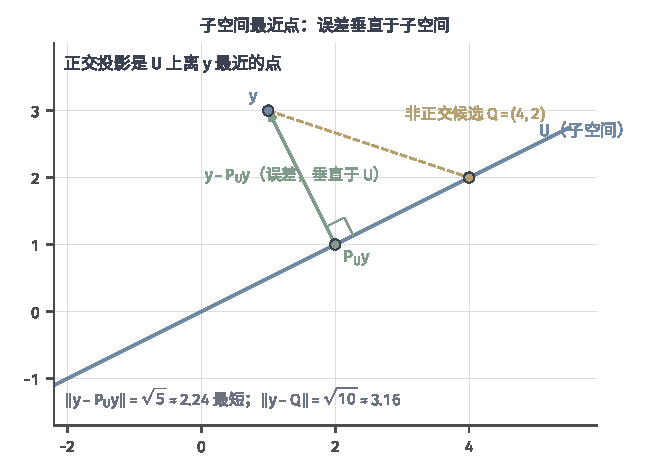
\includegraphics[width=112mm]{figures/01-mathematical-preliminaries-upper/03-linear-spaces/matplotlib/ls-orthogonal-projection-nearest/ls-orthogonal-projection-nearest.pdf}
  \caption{直线子空间$U$（过原点、方向$(2,1)$）上离$\bm y=(1,3)^\top$最近的点是正交投影
  $\bm p=(2,1)^\top$，误差$\bm y-\bm p=(-1,2)^\top$与$U$垂直（直角小方块）；
  同一线上的另一候选$\bm q=(4,2)^\top$到$\bm y$的距离$\sqrt{10}$明显大于最短距离$\sqrt5$。
  这是解析式教学构造。}
  \label{fig:ls-orthogonal-projection-nearest}
\end{figure}

\paragraph{正规方程}

回到矩阵$\bm A$，取$U=\operatorname{range}(\bm A)$，设最近点是$\hat{\bm b}=\bm A\hat{\bm x}$。
列空间由$\bm A$的各列张成，残差$\bm r=\bm b-\bm A\hat{\bm x}$与列空间正交，就是与每一列$\bm a_j$正交，
即$\bm a_j^\top\bm r=0$，$j=1,\ldots,d$，合写为$\bm A^\top\bm r=\bm0$。代入$\bm r$得到\term{正规方程}（normal equations）
\begin{equation}
 \bm A^\top(\bm b-\bm A\hat{\bm x})=\bm0,
 \qquad
 \bm A^\top\bm A\hat{\bm x}=\bm A^\top\bm b.
 \label{eq:linear-algebra-normal-equations}
\end{equation}
“正规”指法向，即残差与列空间正交，不是归一化。由定理~\ref{thm:ls-four-subspaces-orthogonality}，
这也就是说残差落在左零空间$\operatorname{null}(\bm A^\top)$中：最小二乘把$\bm b$分成可达的部分与完全不可达的部分。
下面用一个三个方程、两个未知量的例子计算正规方程。

\begin{example}[超定方程的最小二乘解]
\label{ex:ls-normal-equations-three-by-two}
取$\bm A=\left[\begin{smallmatrix}1&0\\0&1\\1&1\end{smallmatrix}\right]$、$\bm b=(2,3,2)^\top$。
列空间中的向量形如$(x_1,x_2,x_1+x_2)^\top$，第三坐标等于前两坐标之和；而$\bm b$的第三坐标$2\neq2+3$，
所以$\bm b$不在列空间中，方程$\bm A\bm x=\bm b$无解。计算
\[
 \bm A^\top\bm A=\begin{bmatrix}2&1\\1&2\end{bmatrix},\qquad
 \bm A^\top\bm b=\begin{bmatrix}4\\5\end{bmatrix},
\]
解正规方程$2\hat x_1+\hat x_2=4$、$\hat x_1+2\hat x_2=5$，得$\hat{\bm x}=(1,2)^\top$。
最近点为$\bm A\hat{\bm x}=(1,2,3)^\top$，残差为$\bm r=\bm b-\bm A\hat{\bm x}=(1,1,-1)^\top$；
它与两列$(1,0,1)^\top$、$(0,1,1)^\top$的内积都是零，满足正交性判据。
\end{example}

图~\ref{fig:ls-least-squares-residual}画出这个例子。

\begin{figure}[htbp]
  \centering
  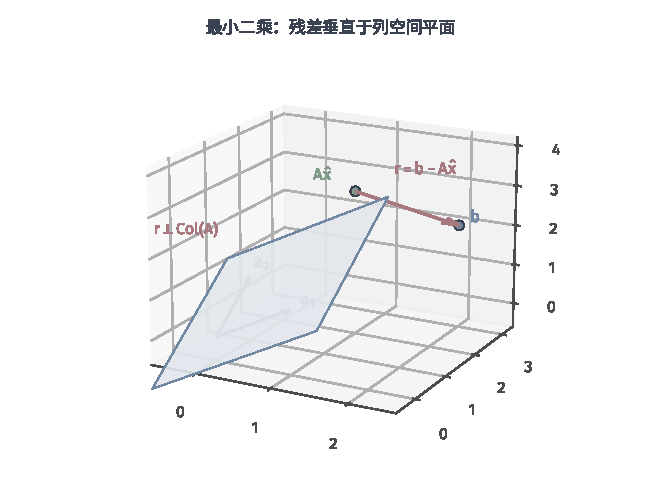
\includegraphics[width=112mm]{figures/01-mathematical-preliminaries-upper/03-linear-spaces/matplotlib/ls-least-squares-residual/ls-least-squares-residual.pdf}
  \caption{列空间平面上的最近点。$\bm A=\left[\begin{smallmatrix}1&0\\0&1\\1&1\end{smallmatrix}\right]$，
  列$\bm a_1=(1,0,1)^\top$、$\bm a_2=(0,1,1)^\top$张成浅蓝平面；$\bm b=(2,3,2)^\top$，
  最近拟合值$\bm A\hat{\bm x}=(1,2,3)^\top$，残差$\bm r=(1,1,-1)^\top$满足
  $\bm r^\top\bm a_1=\bm r^\top\bm a_2=0$。透视教学构造。}
  \label{fig:ls-least-squares-residual}
\end{figure}

正规方程是由几何判据推出的；也可以直接验证，它的解确实使目标取全局最小。设$\hat{\bm x}$满足正规方程，
$\bm r=\bm b-\bm A\hat{\bm x}$，对任意增量$\bm h$，$\bm A(\hat{\bm x}+\bm h)-\bm b=\bm A\bm h-\bm r$，展开平方长度得
\[
 \lVert\bm A(\hat{\bm x}+\bm h)-\bm b\rVert_2^2
 =\lVert\bm r\rVert_2^2-2(\bm A\bm h)^\top\bm r+\lVert\bm A\bm h\rVert_2^2
 =\lVert\bm r\rVert_2^2-2\bm h^\top(\bm A^\top\bm r)+\lVert\bm A\bm h\rVert_2^2 .
\]
正规方程使中间项为零，剩下的$\lVert\bm A\bm h\rVert_2^2\geq0$，所以任何移动都不会减小目标。
反之，若$\hat{\bm x}$是最小点，则拟合值$\bm A\hat{\bm x}$是列空间中离$\bm b$最近的点，由正交性判据，
残差与列空间正交，$\hat{\bm x}$满足正规方程。于是最小二乘问题与正规方程同解，
求最小点就是解这个$d$阶对称线性方程。

用一般子空间的基矩阵$\bm B$代替$\bm A$，并在一般内积下把$\bm B^\top\bm B$的元素换成内积，正规方程成为
\begin{equation}
 \bm G\bm c=\bigl(\langle\bm b_i,\bm y\rangle\bigr)_{i=1}^r,\qquad
 g_{i,j}=\langle\bm b_i,\bm b_j\rangle,
 \label{eq:ls-gram-system}
\end{equation}
系数矩阵$\bm G$是基向量的Gram矩阵；逐行写就是$\sum_j\langle\bm b_i,\bm b_j\rangle c_j=\langle\bm b_i,\bm y\rangle$，
即残差$\bm y-\sum_jc_j\bm b_j$与每个基向量正交。这就把问题~\eqref{eq:ls-nearest-point-coefficients}化成了线性方程。

在示例~\ref{ex:ls-nonorthogonal-coefficients}中，$\bm G=\left[\begin{smallmatrix}2&1\\1&1\end{smallmatrix}\right]$，右端为$(1,0)^\top$，
解得$\bm c=(1,-1)^\top$，与直接观察一致。这里两个基向量张成整个平面，所以最近点就是$\bm y$本身；
Gram系统的作用是把内积$(1,0)^\top$纠正为真正的系数。

基向量标准正交时，Gram矩阵是单位矩阵，Gram系统不必求解：系数就是内积，最近点直接写出，
\[
 \bm p=\sum_j\langle\bm q_j,\bm y\rangle\bm q_j .
\]
这就是第~\ref{chap:linear-representation}章的正交分解公式~\eqref{eq:ls-orthonormal-projection}，每个系数只与自己的方向有关，互不干扰。
它是第~\ref{sec:ls-qr-method}节用QR分解解最小二乘的出发点。

\paragraph{加权最小二乘}
\label{sec:ls-weighted-ls}
\label{sec:ls-weighted-regularized-solve}

上面用欧氏长度度量残差，各个坐标同等对待。不同观测的可靠程度不同时，应让可靠观测的误差付出更大代价。
给定对称正定权重矩阵$\bm M\in\mathbb R^{m\times m}$，\term{加权最小二乘}（weighted least squares）的目标为
\begin{equation}
 \min_{\bm x}\ (\bm A\bm x-\bm b)^\top\bm M(\bm A\bm x-\bm b).
 \label{eq:ls-weighted-objective}
\end{equation}
它用加权内积$\langle\bm u,\bm v\rangle_{\bm M}=\bm u^\top\bm M\bm v$度量残差长度，例如$\bm M$为对角矩阵时，
对角元较大的坐标的误差被惩罚得更重。

$\bm M$对称正定保证这是一个合法内积，
所以正交直和、勾股恒等式与正交性判据原样成立，只是“正交”要按$\bm M$内积判断，最近点一般不同于欧氏情形。
残差与每一列$\bm M$正交，即$\bm a_j^\top\bm M\bm r=0$，合写为$\bm A^\top\bm M\bm r=\bm0$，得到加权正规方程
\begin{equation}
 \bm A^\top\bm M(\bm b-\bm A\hat{\bm x})=\bm0,
 \qquad
 \bm A^\top\bm M\bm A\,\hat{\bm x}=\bm A^\top\bm M\bm b.
 \label{eq:linear-algebra-weighted-normal-equations}
\end{equation}
下面在同一条直线上比较欧氏最近点与加权最近点。

\begin{example}[同一子空间的两种最近点]
\label{ex:linear-algebra-weighted-projection}
在$\mathbb R^2$中取目标$\bm y=(2,1)^\top$、$U=\operatorname{span}\{(1,1)^\top\}$，
最近点写成$a(1,1)^\top$。欧氏情形的正规方程为$(1+1)a=2+1$，即$2a=3$，故$\bm p=(1.5,1.5)^\top$。
改用$\bm M=\operatorname{diag}(1,4)$，加权正规方程为$(1+4)a=2+4$，即$5a=6$，
得到$\bm p_{\bm M}=(1.2,1.2)^\top$。第二坐标的误差代价更大，最近点便向$y_2=1$靠近。
加权残差$\bm y-\bm p_{\bm M}=(0.8,-0.2)^\top$与$(1,1)^\top$的普通内积为$0.6\neq0$，
加权内积为$0.8\cdot1\cdot1+4\cdot(-0.2)\cdot1=0$：它在所选内积下正交，在欧氏内积下不正交。
\end{example}

图~\ref{fig:linear-algebra-weighted-projection}画出这两种最近点。
\begin{figure*}[htbp]
  \centering
  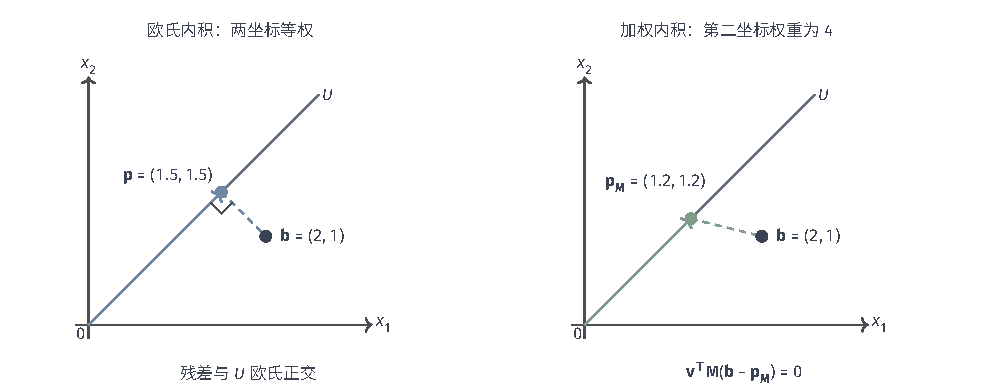
\includegraphics[width=168.998mm]{figures/01-mathematical-preliminaries-upper/03-linear-spaces/tikz/linear-algebra-weighted-projection/figure.pdf}
  \caption{同一目标在同一直线上的欧氏投影与加权投影。实箭头是投影向量，虚线是残差；
  右图画在普通坐标中，残差不必形成欧氏直角。正交性必须用所选内积判断。}
  \label{fig:linear-algebra-weighted-projection}
\end{figure*}

\subsubsection{解的性质}
\label{sec:ls-ls-existence}

最近点$\hat{\bm b}$作为列空间中的点总是存在且唯一，但正规方程的未知量是产生它的输入$\hat{\bm x}$。
本部分回答：这样的输入是否总存在，是否唯一，不唯一时全部解是什么样子，唯一时系数是否可靠。

\paragraph{存在性}

正规方程对任意$\bm b$都有解。几何上这很自然：$\hat{\bm b}$在列空间中，总有输入产生它，而这个输入满足正规方程。
也可以从方程本身验证。先看系数矩阵的零空间：若$\bm A^\top\bm A\bm x=\bm0$，则
$\lVert\bm A\bm x\rVert_2^2=\bm x^\top\bm A^\top\bm A\bm x=0$，即$\bm A\bm x=\bm0$；反向包含显然。故
\begin{equation}
 \ker(\bm A^\top\bm A)=\ker\bm A.
 \label{eq:ls-normal-kernel}
\end{equation}
由定理~\ref{thm:ls-four-subspaces-orthogonality}，对任意矩阵有$\operatorname{range}(\bm A^\top)=(\ker\bm A)^\perp$。把它用在对称矩阵$\bm A^\top\bm A$上，得
$\operatorname{range}(\bm A^\top\bm A)=\ker(\bm A^\top\bm A)^\perp=(\ker\bm A)^\perp=\operatorname{range}(\bm A^\top)$。
右端$\bm A^\top\bm b$显然在$\operatorname{range}(\bm A^\top)$中，所以方程总是相容。

\paragraph{全部解与唯一性}

拟合值唯一，不代表输入唯一。正规方程是相容的线性方程，按第~\ref{sec:ls-uniqueness-freedom}节的结论，它的全部解是一个解加上系数矩阵的零空间；
由~\eqref{eq:ls-normal-kernel}，全部解为
\begin{equation}
 \hat{\bm x}+\ker\bm A.
 \label{eq:ls-all-ordinary-solutions}
\end{equation}
这些解给出同一个拟合值，因为零空间方向不改变输出。于是解唯一当且仅当$\bm A$满列秩。
此时$\bm A^\top\bm A$正定（$\bm x\neq\bm0$时$\bm x^\top\bm A^\top\bm A\bm x=\lVert\bm A\bm x\rVert_2^2>0$），因而可逆，唯一解为
\begin{equation}
 \hat{\bm x}=(\bm A^\top\bm A)^{-1}\bm A^\top\bm b.
 \label{eq:linear-algebra-full-rank-least-squares}
\end{equation}
用子空间的基表示时同样如此：基向量线性无关，Gram矩阵$\bm G$正定，Gram系统~\eqref{eq:ls-gram-system}的解唯一。

这里有两层唯一性要分清。最近点作为$U$中的点总是唯一的；它的系数只在张成向量线性无关时唯一：
若$\bm B\bm c_1=\bm B\bm c_2$，则$\bm B(\bm c_1-\bm c_2)=\bm0$，线性无关迫使$\bm c_1=\bm c_2$。

秩亏时，例如$\bm A$有两列相同，正规方程相容但有无穷多解，第~\ref{sec:ls-select-among-solutions}节的讨论原样适用：
若要求欧氏范数最小，就去掉不改变输出的零空间分量，所得的解落在$(\ker\bm A)^\perp$中，
它也是相容方程$\bm A\bm x=\hat{\bm b}$的最小范数解。
在任意秩下把这一选择写成矩阵需要伪逆，见第~\ref{sec:ls-pseudoinverse}节。

无论解是否唯一，最小值都只由正交分解决定。$\hat{\bm b}\perp\bm r$，勾股恒等式给出
$\lVert\bm b\rVert_2^2=\lVert\hat{\bm b}\rVert_2^2+\lVert\bm r\rVert_2^2$：
观测的平方长度分成被列空间解释的部分与残差部分，最小平方残差
$\lVert\bm r\rVert_2^2=\lVert\bm b\rVert_2^2-\lVert\hat{\bm b}\rVert_2^2$对全部解相同。
示例~\ref{ex:ls-normal-equations-three-by-two}中，$\lVert\bm b\rVert_2^2=17$，$\lVert\hat{\bm b}\rVert_2^2=1+4+9=14$，$\lVert\bm r\rVert_2^2=3$。

\paragraph{唯一不等于稳定}

满列秩只保证系数唯一，不保证系数可靠。下面的例子中，设计矩阵的两列接近共线。

\begin{example}[近共线设计：唯一但不稳定的系数]
\label{ex:ls-nearly-collinear-design}
取互相正交的向量$\bm c_1=(1,1,1)^\top$与$\bm q=(0,1,-1)^\top$。
设计矩阵$\bm X_\varepsilon$的两列为$\bm c_1$与$\bm c_1+\varepsilon\bm q$，响应为$\bm y=\bm c_1+\delta\bm q$。
利用$\bm c_1^\top\bm q=0$、$\lVert\bm c_1\rVert_2^2=3$、$\lVert\bm q\rVert_2^2=2$，正规方程为
\[
 \begin{bmatrix}3&3\\3&3+2\varepsilon^2\end{bmatrix}\hat{\bm w}
 =\begin{bmatrix}3\\3+2\varepsilon\delta\end{bmatrix},
\]
系数矩阵的行列式为$6\varepsilon^2$。$\varepsilon\neq0$时满列秩，解为
\begin{equation}
 \hat{\bm w}_\varepsilon
 =\begin{bmatrix}1-\delta/\varepsilon\\\delta/\varepsilon\end{bmatrix},
 \qquad\bm X_\varepsilon\hat{\bm w}_\varepsilon=\bm y,
 \label{eq:linear-algebra-nearly-collinear-least-squares}
\end{equation}
后一式可直接验证：$(1-\delta/\varepsilon)\bm c_1+(\delta/\varepsilon)(\bm c_1+\varepsilon\bm q)=\bm c_1+\delta\bm q$。
取$\varepsilon=0.01$、$\delta=0.1$，系数为$(-9,10)^\top$，残差却为零。

$\varepsilon=0$时两列重合为$\bm c_1$。此时$\bm y=\bm c_1+\delta\bm q$本身就是正交分解，最近输出为$\bm c_1$，
残差为$\delta\bm q$，平方残差为$2\delta^2$；满足$w_1+w_2=1$的系数都是解。
\end{example}

所以$\delta\neq0$时，随着$\varepsilon\to0$，精确拟合所需的系数趋于无穷，而极限矩阵已经不能精确拟合。
拟合值可以相当稳定，表示它的两个系数却可能很大，而且对$\varepsilon$、$\delta$极为敏感。
这是近共线几何本身的性质，不是计算机舍入造成的；它的定量刻画见第~\ref{sec:ls-ordinary-ls-sensitivity}节。

\paragraph{加权的情形}

加权问题可以化回普通问题。由定理~\ref{thm:ls-gram-factor}，正定$\bm M$可写成
$\bm M=\bm R^\top\bm R$，$\bm R$可逆。于是
$(\bm A\bm x-\bm b)^\top\bm M(\bm A\bm x-\bm b)=\lVert\bm R\bm A\bm x-\bm R\bm b\rVert_2^2$。
令$\tilde{\bm A}=\bm R\bm A$、$\tilde{\bm b}=\bm R\bm b$，加权目标就是普通平方残差$\lVert\tilde{\bm A}\bm x-\tilde{\bm b}\rVert_2^2$，
加权正规方程~\eqref{eq:linear-algebra-weighted-normal-equations}就是$\tilde{\bm A}^\top\tilde{\bm A}\hat{\bm x}=\tilde{\bm A}^\top\tilde{\bm b}$。
这一步常称\term{白化}（whitening）：先用$\bm R$把各坐标的误差变换到同一欧氏尺度。
于是前面的结论都可以搬过来：加权正规方程总有解；$\bm R$可逆使$\ker\tilde{\bm A}=\ker\bm A$，
所以解唯一的条件仍是$\bm A$满列秩。权重只移动最近点，不改变唯一性。

\subsubsection{求解方法}
\label{sec:ls-direct-methods-ls}

最小二乘已经化成正规方程，第一种办法是直接用第~\ref{sec:ls-direct-methods}节的方法解它；
这一办法的弱点在于形成$\bm A^\top\bm A$。第二种办法利用正交变换保持长度，用QR分解绕开$\bm A^\top\bm A$。
本部分假定$\bm A$满列秩，并在精确算术下讨论；有限精度下怎样稳定地算出QR分解，留到第~\ref{sec:ls-truncated-svd-ridge}节。

\paragraph{正规方程法}
\label{sec:ls-normal-equations-method}

最直接的算法是解正规方程。$\bm A$满列秩时$\bm A^\top\bm A$对称正定，可以用Cholesky分解：
先形成$\bm A^\top\bm A$与$\bm A^\top\bm b$，分解$\bm A^\top\bm A=\bm L\bm L^\top$，再依次前代解$\bm L\bm z=\bm A^\top\bm b$、
回代解$\bm L^\top\hat{\bm x}=\bm z$。加权问题对$\bm A^\top\bm M\bm A$作同样的分解。
稠密情形下，形成$\bm A^\top\bm A$约需$md^2$次乘法，分解约需$d^3/3$次运算，多个右端复用同一分解。
$m$远大于$d$时，这是最省的方法。

形成$\bm A^\top\bm A$会损失精度。由第~\ref{sec:ls-svd}节的奇异值分解，$\bm A^\top\bm A$的特征值是$\bm A$的奇异值的平方：
$\bm A$中被压缩得很厉害的方向，在$\bm A^\top\bm A$中被压缩两次，就像一个小数取平方后更小；
浮点计算中，这种方向可能与零无法区分。所以正规方程法只在各列明显线性无关、
$\bm A^\top\bm A$的正定性有充足余量时可靠。秩亏时唯一性本身就不成立；近秩亏时，如示例~\ref{ex:ls-nearly-collinear-design}，
系数本来就不稳定，Cholesky分解成功也不说明结果可用。这种平方造成的精度损失在第~\ref{sec:ls-numerical-sensitivity}节用条件数定量估计。

\paragraph{用QR分解解最小二乘}
\label{sec:ls-qr-method}
\label{sec:linear-algebra-direct-residual}

另一条路线不形成$\bm A^\top\bm A$，而是先给列空间换一组标准正交基。
第~\ref{chap:linear-representation}章的Gram--Schmidt正交化正是做这件事，它把满列秩矩阵写成经济型QR分解
$\bm A=\bm Q\bm R$（式~\eqref{eq:ls-qr-factorization}），$\bm Q$的列是列空间的标准正交基，$\bm R$是对角元为正的上三角矩阵。
QR适合最小二乘的根本原因是：正交矩阵保持欧氏长度，用它变换残差，只改坐标，不改长度，最小点也就不变。

设$\bm A$满列秩，把$\bm Q$的列扩充成$\mathbb R^m$的标准正交基，得到完全QR分解
$\bm A=[\bm Q_1\;\bm Q_2]\left[\begin{smallmatrix}\bm R\\\bm0\end{smallmatrix}\right]=\bm Q_1\bm R$，
其中$[\bm Q_1\;\bm Q_2]$是$m$阶正交矩阵，$\bm Q_1$有$d$列，就是经济型分解中的$\bm Q$；$\bm Q_2$的列张成列空间的正交补。
记$\bm c_1=\bm Q_1^\top\bm b$、$\bm c_2=\bm Q_2^\top\bm b$。用$[\bm Q_1\;\bm Q_2]^\top$变换残差，
\[
 \lVert\bm A\bm x-\bm b\rVert_2^2
 =\left\lVert\begin{bmatrix}\bm R\bm x-\bm c_1\\-\bm c_2\end{bmatrix}\right\rVert_2^2
 =\lVert\bm R\bm x-\bm c_1\rVert_2^2+\lVert\bm c_2\rVert_2^2 .
\]
第二项与$\bm x$无关，是无法消除的残差；第一项可以通过解上三角方程$\bm R\hat{\bm x}=\bm c_1$降为零。
满列秩时$\bm R$的对角元非零，回代即得唯一解，最小平方残差就是$\lVert\bm c_2\rVert_2^2=\lVert\bm b\rVert_2^2-\lVert\bm c_1\rVert_2^2$，
所以$\bm Q_2$不必形成。整个过程不出现$\bm A^\top\bm A$，避免了正规方程法的平方尺度损失，
代价是分解的运算量高于Cholesky。

下面用QR分解重算示例~\ref{ex:ls-normal-equations-three-by-two}。

\begin{example}[用QR分解求解最小二乘]
\label{ex:ls-qr-three-by-two}
仍取$\bm A=\left[\begin{smallmatrix}1&0\\0&1\\1&1\end{smallmatrix}\right]$、$\bm b=(2,3,2)^\top$。
Gram--Schmidt先给出$\bm q_1=(1,0,1)^\top/\sqrt2$。$\bm a_2$在$\bm q_1$上的分量为$r_{1,2}=\bm q_1^\top\bm a_2=1/\sqrt2$，扣除后
\[
 \bm v_2=(0,1,1)^\top-\tfrac12(1,0,1)^\top=(-\tfrac12,1,\tfrac12)^\top,\qquad
 r_{2,2}=\lVert\bm v_2\rVert_2=\sqrt{3/2},
\]
再令$\bm q_2=\bm v_2/r_{2,2}$。于是
\[
 \bm R=\begin{bmatrix}\sqrt2&1/\sqrt2\\0&\sqrt{3/2}\end{bmatrix},\qquad
 \bm c_1=\begin{bmatrix}\bm q_1^\top\bm b\\\bm q_2^\top\bm b\end{bmatrix}=\begin{bmatrix}2\sqrt2\\\sqrt6\end{bmatrix}.
\]
回代解$\bm R\hat{\bm x}=\bm c_1$，得$\hat x_2=\sqrt6/\sqrt{3/2}=2$、$\hat x_1=(2\sqrt2-2/\sqrt2)/\sqrt2=1$，
与正规方程的结果相同。最小平方残差为$\lVert\bm b\rVert_2^2-\lVert\bm c_1\rVert_2^2=17-(8+6)=3$，也与前面一致。
\end{example}

同一分解还给出最近点。最近点为$\hat{\bm b}=\bm A\hat{\bm x}=\bm Q_1\bm R\hat{\bm x}=\bm Q_1\bm c_1=\bm Q_1\bm Q_1^\top\bm b$，
$\bm c_1$的分量就是$\bm b$在各正交方向上的坐标，不必另解Gram系统。

它也判定相容性：$\bm c_2=\bm0$当且仅当$\bm b$在列空间中，
此时回代得到的就是原方程的精确解；$\bm c_2\neq\bm0$时原方程不相容，$\lVert\bm c_2\rVert_2$就是$\bm b$到列空间的距离。
例如$\bm A=\left[\begin{smallmatrix}1&1\\1&0\\0&1\end{smallmatrix}\right]$、$\bm b=(2,1,1)^\top=\bm A(1,1)^\top$时$\bm c_2=\bm0$，
回代得到精确解$\hat{\bm x}=(1,1)^\top$。这就是第~\ref{sec:ls-direct-methods}节所说的：
超定而满列秩的方程，相容性的判断与唯一解的计算可以由同一个QR分解一次完成。

$\bm A$秩亏时，Gram--Schmidt在某一列得不到新方向，$\bm R$不再可逆，上面的回代不能直接进行；
这时最小二乘解不唯一，最小范数解由第~\ref{sec:ls-pseudoinverse}节的伪逆给出。
有限精度下怎样借带列主元的QR判断秩，见第~\ref{sec:ls-orthogonalization-qr}节。

\subsubsection{投影矩阵}
\label{sec:ls-projection-matrices}

求出的最近点随目标线性变化：$\bm y_1,\bm y_2$的正交分解相加、数乘后仍是正交分解，由分解的唯一性，
最近点也随之相加、数乘。所以$\bm y\mapsto\bm p$是一个线性映射，称为到$U$的正交投影。
本部分把它写成矩阵，并回答：拿到一个矩阵，怎样判断它是不是正交投影。

\paragraph{正交投影、斜投影与幂等}

设$\bm Q$的列是$U$的标准正交基。由$\bm p=\sum_j\langle\bm q_j,\bm y\rangle\bm q_j=\bm Q\bm Q^\top\bm y$，
标准内积下到$U$的正交投影是
\begin{equation}
 \bm P_U=\bm Q\bm Q^\top,\qquad
 \bm P_U^\top=\bm P_U,\qquad \bm P_U^2=\bm P_U.
 \label{eq:linear-algebra-orthogonal-projector}
\end{equation}
两条性质都可以直接验证。由$\bm Q^\top\bm Q=\bm I$，$\bm P_U^2=\bm Q(\bm Q^\top\bm Q)\bm Q^\top=\bm Q\bm Q^\top$，
即幂等：已经在$U$中的点再投影一次不变。$(\bm Q\bm Q^\top)^\top=\bm Q\bm Q^\top$，即对称。
此外$\operatorname{range}\bm P_U=\operatorname{range}\bm Q=U$。

幂等性只说明这是某种投影，并不说明是最近点映射。一般的幂等矩阵$\bm P$把$\bm y$分成$\bm P\bm y$与
$\bm y-\bm P\bm y$两部分，前者在像中，后者在零空间中（因为$\bm P(\bm y-\bm P\bm y)=\bm P\bm y-\bm P^2\bm y=\bm0$），
但两部分不必正交。这种映射称为\term{斜投影}（oblique projection）。

\begin{example}[反例：幂等而不对称的投影]
\label{ex:ls-oblique-projection}
取$\bm P=\left[\begin{smallmatrix}1&-1\\0&0\end{smallmatrix}\right]$。直接相乘得$\bm P^2=\bm P$，所以它幂等；
它把$(y_1,y_2)^\top$送到$x$轴上的$(y_1-y_2,0)^\top$。残差$\bm y-\bm P\bm y=(y_2,y_2)^\top$与$x$轴方向$(1,0)^\top$的内积是$y_2$，
$y_2\neq0$时不为零，所以$\bm P\bm y$不是$x$轴上离$\bm y$最近的点。这个$\bm P$也不对称：$\bm P^\top\neq\bm P$。
\end{example}

对称性正是正交的条件：若$\bm P$幂等且对称，对任意$\bm y,\bm z$有
$(\bm y-\bm P\bm y)^\top\bm P\bm z=\bm y^\top(\bm P-\bm P^\top\bm P)\bm z=\bm y^\top(\bm P-\bm P^2)\bm z=0$，
残差与整个像正交，由正交性判据，$\bm P$就是到其像的正交投影。
所以判别分两步：先验幂等，判断是不是投影；再验对称，判断是不是正交投影。

\paragraph{列空间投影与正规方程}

不做正交化，也可以从正规方程写出投影矩阵。$\bm A$满列秩时，最近点为
$\hat{\bm b}=\bm A\hat{\bm x}=\bm A(\bm A^\top\bm A)^{-1}\bm A^\top\bm b$，故
\begin{equation}
 \bm P_{\operatorname{range}(\bm A)}=\bm A(\bm A^\top\bm A)^{-1}\bm A^\top.
 \label{eq:ls-column-space-projector}
\end{equation}
直接相乘可验它对称且幂等。代入$\bm A=\bm Q\bm R$，得$\bm Q\bm R(\bm R^\top\bm R)^{-1}\bm R^\top\bm Q^\top=\bm Q\bm Q^\top$，
与式~\eqref{eq:linear-algebra-orthogonal-projector}一致，说明投影只取决于列空间，与所用的基无关。

回归中这个矩阵常称帽子矩阵，它把观测$\bm y$映成拟合值$\hat{\bm y}$；$\bm I-\bm P$则把观测映成残差，
它是到$\operatorname{range}(\bm A)^\perp=\operatorname{null}(\bm A^\top)$的正交投影。
加权内积下，同样的推导给出$\bm A(\bm A^\top\bm M\bm A)^{-1}\bm A^\top\bm M$；它幂等但一般不对称，
在普通内积下是斜投影，在$\bm M$内积下才是正交投影。

两个正交投影相乘一般不可交换，$\bm P_U\bm P_V\neq\bm P_V\bm P_U$，乘积也未必还是投影。
两者可交换时，乘积既幂等又对称，因而是到其像的正交投影。它的像含于$U$（左因子是$\bm P_U$），
也含于$V$（交换次序后左因子是$\bm P_V$），而$U\cap V$中的向量被它保持不变，所以它是到$U\cap V$的正交投影。

\subsubsection{结果核验}
\label{sec:ls-least-squares-verification}

最小二乘的残差一般不为零，所以“残差小”不能作为合格标准；合格标准是残差与列空间正交。
算出$\hat{\bm x}$后分别核验三项。第一，正规方程残差$\bm g=\bm A^\top(\bm b-\bm A\hat{\bm x})$是否在容限内为零，
它检验的正是正交性判据。第二，输出残差$\bm r=\bm b-\bm A\hat{\bm x}$的长度，它是$\bm b$到列空间的距离，
说明模型能解释观测到什么程度。第三，若要求最小范数解，检查$\hat{\bm x}$是否与$\ker\bm A$正交。

用示例~\ref{ex:ls-normal-equations-three-by-two}核对：$\hat{\bm x}=(1,2)^\top$时$\bm r=(1,1,-1)^\top$，$\bm A^\top\bm r=(0,0)^\top$，第一项通过；
$\lVert\bm r\rVert_2=\sqrt3$，这是无法再减小的距离；$\bm A$满列秩，$\ker\bm A=\{\bm0\}$，第三项自动满足。

加权问题按原目标核验：检查加权正规方程~\eqref{eq:linear-algebra-weighted-normal-equations}的残差
$\bm A^\top\bm M(\bm b-\bm A\hat{\bm x})$，并报告$\bm M$加权的残差长度。白化后的残差（用$\bm M=\bm R^\top\bm R$的因子$\bm R$变换后的$\bm R\bm r$）与它长度相同，
但坐标已经变换，不能当作原观测的残差逐项解读。

\subsection{伪逆}
\label{sec:ls-pseudoinverse}

到这里，三种情况各有各的答案。$\bm A$可逆时，唯一解是$\bm A^{-1}\bm b$；满行秩而有无穷多解时，
最小范数解是$\bm A^\top(\bm A\bm A^\top)^{-1}\bm b$；满列秩而无解时，最小二乘解是$(\bm A^\top\bm A)^{-1}\bm A^\top\bm b$。
三个公式各自要求一种满秩，而一般的$\bm A$可能既不满行秩、也不满列秩，这时方程可能无解，
最小二乘解又不唯一，需要先取最近点、再在最近点的全部原像中取范数最小者。
本小节用第~\ref{chap:linear-analysis}章的奇异值分解构造一个矩阵$\bm A^\dagger$，
使$\bm A^\dagger\bm b$在任何秩下都给出这样两次选择的结果，再说明前面三个公式都是它的特例。

\paragraph{用奇异值分解构造}

设$\bm A\in\mathbb R^{m\times d}$的秩为$r$，奇异值分解为~\eqref{eq:matrix-analysis-svd-rank-one-sum}，
$\sigma_1\geq\cdots\geq\sigma_r>0$；按第~\ref{sec:ls-svd}节的构造，把$\bm u_1,\ldots,\bm u_r$与$\bm v_1,\ldots,\bm v_r$
分别扩充为$\mathbb R^m$与$\mathbb R^d$的标准正交基。那里已经说明，$\operatorname{range}(\bm A)$由$\bm u_1,\ldots,\bm u_r$张成，
$\ker\bm A$由$\bm v_{r+1},\ldots,\bm v_d$张成。

$\bm A$把$\bm v_i$伸缩为$\sigma_i\bm u_i$，反向自然应把$\bm u_i$送回$\bm v_i/\sigma_i$。
按两次选择的要求分配$\bm b$的各个分量：把$\bm b$按$\bm u_i$展开，分量$\bm u_i^\top\bm b$（$i\leq r$）配给$\bm v_i/\sigma_i$；
落在$\operatorname{range}(\bm A)^\perp$中的分量（$i>r$）没有原像，直接丢弃，这对应取最近点；
零空间方向$\bm v_{r+1},\ldots,\bm v_d$不分配任何分量，这对应在原像中取范数最小者。

\begin{definition}[Moore--Penrose伪逆]
\label{def:matrix-analysis-pseudoinverse}
设$\bm A$有奇异值分解~\eqref{eq:matrix-analysis-svd-rank-one-sum}。$\bm A$的\term{Moore--Penrose伪逆}（Moore--Penrose pseudoinverse）为
\begin{equation}
 \bm A^\dagger=\sum_{i=1}^r\frac{1}{\sigma_i}\bm v_i\bm u_i^\top,
 \label{eq:matrix-analysis-pseudoinverse}
\end{equation}
$\bm A=\bm0$时规定$\bm A^\dagger=\bm0$。
\end{definition}

下面的定理说明，这样构造的矩阵恰好完成了上面的两次选择。
\begin{theorem}[最小二乘与最小范数]
\label{thm:matrix-analysis-pseudoinverse-minimum-norm}
给定$\bm A\in\mathbb R^{m\times d}$和$\bm b\in\mathbb R^m$，全部最小二乘解为
\begin{equation}
 \hat{\bm x}=\bm A^\dagger\bm b+\bm z,
 \qquad \bm z\in\ker\bm A,
 \label{eq:ls-all-pseudoinverse-solutions}
\end{equation}
其中$\bm A^\dagger\bm b$是唯一的最小欧氏范数解；方程相容时，它就是全部精确解中范数最小者。
\end{theorem}
\begin{proof}
把$\bm b$与$\bm x$分别按左、右奇异向量展开，记$b_i=\bm u_i^\top\bm b$、$c_i=\bm v_i^\top\bm x$。由$\bm A\bm x=\sum_{i\leq r}\sigma_ic_i\bm u_i$与$\bm u_1,\ldots,\bm u_m$标准正交，
\[
 \lVert\bm A\bm x-\bm b\rVert_2^2
 =\sum_{i=1}^r(\sigma_ic_i-b_i)^2+\sum_{i=r+1}^m b_i^2 .
\]
第二项与$\bm x$无关；第一项当且仅当$c_i=b_i/\sigma_i$（$i\leq r$）时为零，而$c_{r+1},\ldots,c_d$可以任取。前者正是$\bm A^\dagger\bm b$的坐标，后者组成$\ker\bm A$中的任意向量，所以最小二乘解恰为$\bm A^\dagger\bm b+\bm z$，$\bm z\in\ker\bm A$。由于$\bm A^\dagger\bm b$只含$\bm v_1,\ldots,\bm v_r$方向，它与$\bm z$正交，$\lVert\bm x\rVert_2^2=\lVert\bm A^\dagger\bm b\rVert_2^2+\lVert\bm z\rVert_2^2$，最小值仅在$\bm z=\bm0$时达到。方程相容时第二项为零，最小二乘解就是精确解，论证不变。
\end{proof}

\paragraph{三种情况的统一}

定理对$\bm A$的秩和$\bm b$的位置都没有要求，所以前面分别处理的情况都包含在其中。
方程相容时，最近点就是$\bm b$本身，$\bm A^\dagger\bm b$是精确解中范数最小的一个：解唯一时它就是那个解，
有无穷多解时它就是第~\ref{sec:ls-select-among-solutions}节的最小范数解。方程无解时，$\bm A^\dagger\bm b$是最小二乘解；
最小二乘解唯一时它就是那一个，不唯一时它是其中范数最小者。

三个满秩公式由此成为特例。$\bm A$满列秩时$\ker\bm A=\{\bm0\}$，最小二乘解唯一，
所以对每个$\bm b$都有$\bm A^\dagger\bm b=(\bm A^\top\bm A)^{-1}\bm A^\top\bm b$，即$\bm A^\dagger=(\bm A^\top\bm A)^{-1}\bm A^\top$。
$\bm A$满行秩时每个右端都相容，$\bm A^\dagger\bm b$是最小范数精确解，由第~\ref{sec:ls-select-among-solutions}节，
$\bm A^\dagger=\bm A^\top(\bm A\bm A^\top)^{-1}$。$\bm A$可逆时两种情形同时成立，两个公式都化为$\bm A^{-1}$，所以$\bm A^\dagger=\bm A^{-1}$。
下面用一个欠定方程核对满行秩的情形。

\begin{example}[欠定方程的伪逆]
\label{ex:ls-pinv-underdetermined}
欠定方程$2x_1=3$的系数矩阵$\bm A=[2\ 0]$满行秩，右端$\bm b=(3)$。$\bm A$的奇异值分解只有一项：
$\sigma_1=2$、$\bm u_1=(1)$、$\bm v_1=(1,0)^\top$。和式~\eqref{eq:matrix-analysis-pseudoinverse}给出
\[
 \bm A^\dagger=\frac12\bm v_1\bm u_1^\top=\begin{bmatrix}1/2\\0\end{bmatrix},
\]
与满行秩公式$\bm A^\top(\bm A\bm A^\top)^{-1}=(2,0)^\top/4$一致。$\bm A^\dagger\bm b=(3/2,0)^\top$
正是全部解$(3/2,t)^\top$中范数最小的一个。
\end{example}

秩亏而又不相容时，两次选择都真正起作用，满秩公式一个也用不上。

\begin{example}[秩亏且不相容时的两次选择]
\label{ex:ls-pinv-two-selections}
取$\bm A=\left[\begin{smallmatrix}1&1\\0&0\end{smallmatrix}\right]$、$\bm b=(2,1)^\top$。$\bm A$的秩为$1$，既不满行秩，也不满列秩。
可达输出都形如$(s,0)^\top$，其中离$\bm b$最近的是$(2,0)^\top$，残差$(0,1)^\top$无法消除。
$(2,0)^\top$的原像是直线$x_1+x_2=2$，由示例~\ref{ex:ls-min-norm-line}，其上最靠近原点的点是$(1,1)^\top$。
用和式核对：$\bm A$只有一个正奇异值$\sigma_1=\sqrt2$，对应$\bm u_1=(1,0)^\top$、$\bm v_1=(1,1)^\top/\sqrt2$，于是
\[
 \bm A^\dagger=\frac1{\sqrt2}\bm v_1\bm u_1^\top=\frac12\begin{bmatrix}1&0\\1&0\end{bmatrix},\qquad
 \bm A^\dagger\bm b=\begin{bmatrix}1\\1\end{bmatrix}.
\]
两次选择的结果与和式一致。
\end{example}

图~\ref{fig:matrix-analysis-pseudoinverse-selections}画出这两次选择。
伪逆既没有让无解的方程变得可解，也没有恢复被$\bm A$消去的信息，它只是在两处都作了最小化选择。

\begin{figure*}[htbp]
  \centering
  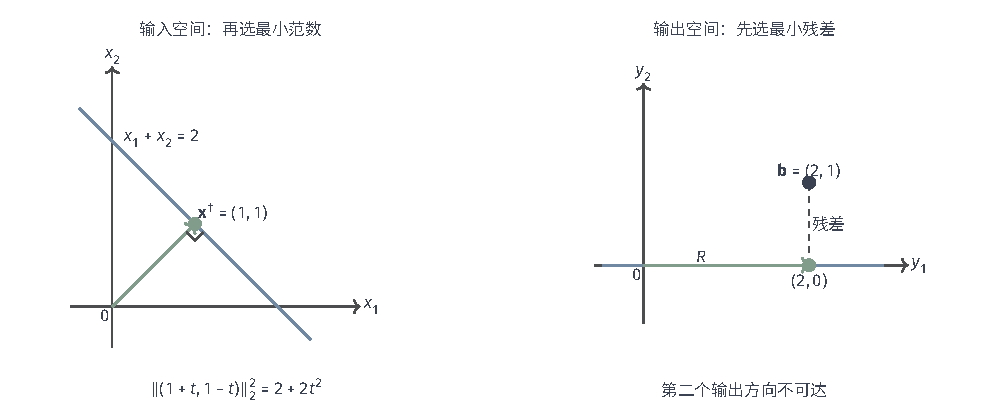
\includegraphics[width=168.998mm]{figures/01-mathematical-preliminaries-upper/03-linear-spaces/tikz/matrix-analysis-pseudoinverse-selections/figure.pdf}
  \caption{伪逆的两次选择。右图先在可达输出中选择离$\bm b=(2,1)^\top$最近的
  $(2,0)^\top$；左图再在整条原像直线$x_1+x_2=2$上选择最靠近原点的$(1,1)^\top$。
  两图属于不同空间，各自等比例绘制。}
  \label{fig:matrix-analysis-pseudoinverse-selections}
\end{figure*}

\paragraph{两个投影与Penrose条件}

两次选择也可以用投影矩阵表达。由和式直接相乘，
\[
 \bm A\bm A^\dagger=\sum_{i\leq r}\bm u_i\bm u_i^\top,\qquad
 \bm A^\dagger\bm A=\sum_{i\leq r}\bm v_i\bm v_i^\top ,
\]
前者是到$\operatorname{range}(\bm A)$的正交投影，后者是到$(\ker\bm A)^\perp=\operatorname{range}(\bm A^\top)$的正交投影
（式~\eqref{eq:linear-algebra-orthogonal-projector}）。也就是说，$\bm A^\dagger$先把输出正交投影到$\operatorname{range}(\bm A)$，
再在$\operatorname{range}(\bm A^\top)$上反演$\bm A$。

奇异值分解并不唯一，伪逆却不依赖分解的具体选取。由上面两个投影，$\bm A^\dagger$满足四条Penrose条件：
\[
 \bm A\bm A^\dagger\bm A=\bm A,\quad
 \bm A^\dagger\bm A\bm A^\dagger=\bm A^\dagger,\quad
 (\bm A\bm A^\dagger)^\top=\bm A\bm A^\dagger,\quad
 (\bm A^\dagger\bm A)^\top=\bm A^\dagger\bm A .
\]
满足这四条的矩阵只有一个，所以无论用哪个奇异值分解代入和式，得到的都是同一个矩阵。

下面证明唯一性。设$\bm G$也满足四条条件。由第一条，$(\bm A\bm G)^2=(\bm A\bm G\bm A)\bm G=\bm A\bm G$，即$\bm A\bm G$幂等，
且$\operatorname{range}(\bm A\bm G)=\operatorname{range}(\bm A)$（$\subseteq$显然，$\supseteq$由$\bm A=\bm A\bm G\bm A$）；
同理$\bm G\bm A$幂等，且$\ker(\bm G\bm A)=\ker\bm A$（$\supseteq$显然，$\subseteq$由$\bm A=\bm A\bm G\bm A$）。
后两条说明它们对称，而由第~\ref{sec:ls-projection-matrices}节，对称的幂等矩阵就是到其像的正交投影。
$\bm A\bm G$与$\bm A\bm A^\dagger$都是到$\operatorname{range}(\bm A)$的正交投影，所以$\bm A\bm G=\bm A\bm A^\dagger$。
对称矩阵的像是其零空间的正交补，所以$\bm G\bm A$与$\bm A^\dagger\bm A$都是到$(\ker\bm A)^\perp$的正交投影，$\bm G\bm A=\bm A^\dagger\bm A$。再由第二条，
\[
 \bm G=\bm G\bm A\bm G=(\bm A^\dagger\bm A)\bm G=\bm A^\dagger(\bm A\bm G)=\bm A^\dagger\bm A\bm A^\dagger=\bm A^\dagger .
\]

至此，三种情况的答案统一为$\bm A^\dagger\bm b$。实际计算中，满秩时仍用前面各小节基于分解的方法，
不必为此计算奇异值分解；伪逆的作用在于给出一个对任何秩都成立的统一描述。

不过伪逆有一个与逆矩阵不同的性质：它关于矩阵不连续。非零标量$\varepsilon$的伪逆是$1/\varepsilon$，零的伪逆却是$0$，
$\varepsilon\to0$时前者趋于无穷，而不是趋于后者。原因在于和式中的增益$1/\sigma_i$：小奇异值被放大成大增益。
数据带有误差时，这种放大意味着什么，是下一小节要回答的问题。

\subsection{数值敏感性}
\label{sec:ls-numerical-sensitivity}

前面各小节都假定$\bm A$与$\bm b$精确，并在精确算术下求解。实际数据带有测量误差，计算又有舍入误差，
所以还要问：输入有一点误差时，算出的解会偏离多少？残差小时，解是否就准确？
第~\ref{chap:linear-analysis}章已经回答了最简单的情形：可逆方程只有右端带误差时，
解的相对误差不超过条件数$\kappa(\bm A)$乘右端的相对误差（定理~\ref{thm:matrix-analysis-condition-number-bound}），
而在欧氏范数下$\kappa_2(\bm A)$是最大与最小奇异值之比。本小节从这里出发，先处理系数矩阵也带误差的情形，
再说明真解未知时怎样由残差判断算出的解，然后分析最小二乘的三类输出。分析会显示，误差放大的根源都在小奇异值，
求解方法还可能额外放大误差；最后据此介绍数据与计算两方面的改进。

\subsubsection{方程解的敏感度}
\label{sec:ls-equation-sensitivity}
\label{sec:ls-linear-system-sensitivity}

\paragraph{右端扰动}

先看只改右端的情形。设$\bm A$可逆，右端由$\bm b$变为$\bm b+\Delta\bm b$，解的变化为$\Delta\bm x=\bm A^{-1}\Delta\bm b$。
由$\lVert\bm A^{-1}\rVert_2=1/\sigma_{\min}(\bm A)$，右端误差落在小奇异值方向时被放大$1/\sigma_{\min}$倍；
换成相对误差，放大倍数不超过$\kappa(\bm A)$。下面用两个$2\times2$例子对照。

\begin{example}[良态方程的右端扰动]
\label{ex:ls-rhs-perturbation-well-conditioned}
取$\bm A_1=\operatorname{diag}(2,1)$，$\kappa_2(\bm A_1)=2$。右端由$(2,1)^\top$改为$(2,1.01)^\top$，解由$(1,1)^\top$变为$(1,1.01)^\top$。
两者的相对变化分别为
\[
 \frac{\lVert\Delta\bm b\rVert_2}{\lVert\bm b\rVert_2}=\frac{0.01}{\sqrt5}\approx0.00447,\qquad
 \frac{\lVert\Delta\bm x\rVert_2}{\lVert\bm x\rVert_2}=\frac{0.01}{\sqrt2}\approx0.00707,
\]
放大约$1.58$倍，不超过$\kappa_2(\bm A_1)=2$。
\end{example}

\begin{example}[近平行列的右端扰动]
\label{ex:ls-rhs-perturbation-near-parallel}
取$\bm A_2=\left[\begin{smallmatrix}1&1\\0&\varepsilon\end{smallmatrix}\right]$，$0<\varepsilon\ll1$，两列接近同向。
$\bm A_2^\top\bm A_2=\left[\begin{smallmatrix}1&1\\1&1+\varepsilon^2\end{smallmatrix}\right]$的迹为$2+\varepsilon^2$、行列式为$\varepsilon^2$，
两个特征值约为$2$与$\varepsilon^2/2$，所以$\sigma_{\max}\approx\sqrt2$、$\sigma_{\min}\approx\varepsilon/\sqrt2$，$\kappa_2(\bm A_2)\approx2/\varepsilon$。

取$\varepsilon=10^{-2}$、$\bm b=(2,0)^\top$，解为$(2,0)^\top$。只把$\bm b$的第二分量改为$\eta=10^{-2}$，
由$\varepsilon x_2=\eta$与$x_1+x_2=2$得新解$(1,1)^\top$。两者的相对变化分别为
\[
 \frac{\lVert\Delta\bm b\rVert_2}{\lVert\bm b\rVert_2}=\frac{\eta}{2}=0.005,\qquad
 \frac{\lVert\Delta\bm x\rVert_2}{\lVert\bm x\rVert_2}=\frac{\lVert(-1,1)^\top\rVert_2}{\lVert(2,0)^\top\rVert_2}=\frac{\sqrt2}{2}\approx0.707,
\]
放大约$141$倍，与$\kappa_2(\bm A_2)\approx200$同量级。
\end{example}

两个例子都没有舍入误差，差别完全来自问题本身。第二例中解的变化$(-1,1)^\top$几乎正沿着$\bm A_2$的小奇异值方向，
所以被放大得最多。

\paragraph{逆矩阵的扰动}
\label{sec:ls-inverse-sensitivity}
\label{sec:ch06-inverse-stability}

$\bm A$本身也带误差时，扰动后的矩阵甚至可能不再可逆。所以设$\bm B=\bm A+\bm E$，要先回答两件事：
$\bm B$是否可逆，$\bm B^{-1}$离$\bm A^{-1}$多远。答案会给出一个“到奇异边界的余量”。

先看可逆性。若$\lVert\bm A^{-1}\bm E\rVert<1$，则$\bm B$可逆。假设$\bm B\bm x=\bm0$，即$\bm A\bm x=-\bm E\bm x$，左乘$\bm A^{-1}$得$\bm x=-\bm A^{-1}\bm E\bm x$，取范数得$\lVert\bm x\rVert\leq\lVert\bm A^{-1}\bm E\rVert\lVert\bm x\rVert$，这只在$\bm x=\bm0$时可能，所以$\ker\bm B=\{\bm0\}$。

再看逆的变化。由$\bm B^{-1}(\bm A-\bm B)\bm A^{-1}=\bm B^{-1}-\bm A^{-1}$，逆差满足精确恒等式
\begin{equation}
 \bm B^{-1}-\bm A^{-1}
 =-\bm B^{-1}\bm E\,\bm A^{-1}.
 \label{eq:ch06-inverse-finite-perturbation}
\end{equation}
右端含有未知的$\bm B^{-1}$，需要先估计它的大小。

对任意$\bm y$，令$\bm x=\bm B^{-1}\bm y$，由$\bm A\bm x=\bm y-\bm E\bm x$得$\bm x=\bm A^{-1}\bm y-\bm A^{-1}\bm E\bm x$，取范数并移项，$\lVert\bm x\rVert\leq\lVert\bm A^{-1}\rVert\lVert\bm y\rVert/(1-\lVert\bm A^{-1}\bm E\rVert)$，即
\[
 \lVert\bm B^{-1}\rVert\leq\frac{\lVert\bm A^{-1}\rVert}{1-\lVert\bm A^{-1}\bm E\rVert}.
\]
代入恒等式，$\lVert\bm B^{-1}-\bm A^{-1}\rVert\leq\lVert\bm B^{-1}\rVert\lVert\bm E\rVert\lVert\bm A^{-1}\rVert$。两边除以$\lVert\bm A^{-1}\rVert$，再用$\lVert\bm A^{-1}\bm E\rVert\leq\lVert\bm A^{-1}\rVert\lVert\bm E\rVert=\kappa(\bm A)\lVert\bm E\rVert/\lVert\bm A\rVert$，得
\[
 \frac{\lVert\bm B^{-1}-\bm A^{-1}\rVert}
      {\lVert\bm A^{-1}\rVert}
 \leq
 \frac{\kappa(\bm A)\,\lVert\bm E\rVert/\lVert\bm A\rVert}
      {1-\kappa(\bm A)\,\lVert\bm E\rVert/\lVert\bm A\rVert}.
\]
分子是条件数乘相对扰动，分母是到奇异边界的余量。$\kappa(\bm A)\lVert\bm E\rVert/\lVert\bm A\rVert$接近$1$时界急剧变大；
它不小于$1$时本界失效，但这不等于$\bm B$一定奇异。下面的对角例子说明，这个界可以取等号，余量趋于零时逆矩阵的变化确实无界。

\begin{example}[接近奇异边界的对角矩阵]
\label{ex:ls-inverse-perturbation-diagonal}
取$\bm A=\operatorname{diag}(1,\varepsilon)$，$0<\varepsilon<1$，则$\kappa_2(\bm A)=1/\varepsilon$。
令$\bm E=\operatorname{diag}(0,-\delta)$，$0<\delta<\varepsilon$，即把第二个对角元减少$\delta$。
逆矩阵的该元由$1/\varepsilon$变为$1/(\varepsilon-\delta)$，相对变化为
\[
 \frac{\lVert\bm B^{-1}-\bm A^{-1}\rVert_2}{\lVert\bm A^{-1}\rVert_2}
 =\frac{1/(\varepsilon-\delta)-1/\varepsilon}{1/\varepsilon}
 =\frac{\delta}{\varepsilon-\delta}.
\]
扰动的相对大小为$\lVert\bm E\rVert_2/\lVert\bm A\rVert_2=\delta$，于是$\kappa_2(\bm A)\lVert\bm E\rVert_2/\lVert\bm A\rVert_2=\delta/\varepsilon$，
上界为$(\delta/\varepsilon)/(1-\delta/\varepsilon)=\delta/(\varepsilon-\delta)$，与实际变化恰好相等。
$\delta\to\varepsilon$时相对变化无界：扰动的相对大小接近$1/\kappa_2(\bm A)=\varepsilon$时，矩阵到达奇异边界。
\end{example}

\paragraph{矩阵与右端同时扰动}

有了逆矩阵的估计，就可以处理一般情形。设$(\bm A+\bm E)(\bm x+\Delta\bm x)=\bm b+\Delta\bm b$，减去$\bm A\bm x=\bm b$，得$\bm A\Delta\bm x=\Delta\bm b-\bm E\bm x-\bm E\Delta\bm x$。左乘$\bm A^{-1}$并取范数，
\[
 \lVert\Delta\bm x\rVert\leq\lVert\bm A^{-1}\rVert\bigl(\lVert\Delta\bm b\rVert+\lVert\bm E\rVert\lVert\bm x\rVert+\lVert\bm E\rVert\lVert\Delta\bm x\rVert\bigr).
\]
把含$\lVert\Delta\bm x\rVert$的项移到左边，两边除以$\lVert\bm x\rVert$，并用$\lVert\Delta\bm b\rVert/\lVert\bm x\rVert\leq\lVert\bm A\rVert\lVert\Delta\bm b\rVert/\lVert\bm b\rVert$，在$\kappa(\bm A)\lVert\bm E\rVert/\lVert\bm A\rVert<1$时得到
\begin{equation}
 \frac{\lVert\Delta\bm x\rVert}{\lVert\bm x\rVert}
 \leq
 \frac{\kappa(\bm A)}{1-\kappa(\bm A)\lVert\bm E\rVert/\lVert\bm A\rVert}
 \left(
 \frac{\lVert\Delta\bm b\rVert}{\lVert\bm b\rVert}
 +\frac{\lVert\bm E\rVert}{\lVert\bm A\rVert}
 \right).
 \label{eq:matrix-analysis-linear-system-perturbation}
\end{equation}
读法是：两类相对扰动先相加，再被条件数放大，最后除以到奇异边界的余量。
$\bm E=\bm0$时它退回定理~\ref{thm:matrix-analysis-condition-number-bound}的右端扰动界。
这仍是最坏方向上的上界；扰动是否落在放大方向，决定实际误差离这个上界有多远。

\subsubsection{残差与后向误差}
\label{sec:ls-numerical-stability}
\label{sec:ls-data-computation-error}
\label{sec:linear-algebra-error-propagation}
\label{sec:ch06-error-propagation}
\label{sec:ls-result-verification}
\label{sec:matrix-analysis-error-verification}

上面的界比较的是两个精确解。实际手里只有一个算出的候选解$\widehat{\bm x}$，真解未知，怎样判断它的误差？
第~\ref{sec:ls-linear-equation-verification}节用残差核验候选解，并提醒残差小不等于解准确；现在可以定量说明这一点。能直接计算的是残差
\begin{equation}
 \bm r=\bm b-\bm A\widehat{\bm x}.
 \label{eq:matrix-analysis-residual}
\end{equation}
由$\bm A(\bm x-\widehat{\bm x})=\bm r$，候选解的误差是$\bm A^{-1}\bm r$，与只改右端的情形相同，相对误差满足
\[
 \frac{\lVert\widehat{\bm x}-\bm x\rVert}{\lVert\bm x\rVert}
 \leq\kappa(\bm A)\frac{\lVert\bm r\rVert}{\lVert\bm b\rVert}.
\]
所以病态时小残差不保证解准确，下面的例子把这一点推到极端。

\begin{example}[反例：残差小而解误差大]
\label{ex:ls-small-residual-large-error}
取$\bm A=\operatorname{diag}(1,\varepsilon)$、$\bm b=(1,\varepsilon)^\top$，$0<\varepsilon\ll1$，精确解为$\bm x=(1,1)^\top$。
候选解$\widehat{\bm x}=(1,0)^\top$的残差为$\bm r=(0,\varepsilon)^\top$，相对残差为$\varepsilon/\sqrt{1+\varepsilon^2}$，随$\varepsilon\to0$趋于零；
相对解误差却是$\lVert(0,-1)^\top\rVert_2/\lVert(1,1)^\top\rVert_2=1/\sqrt2$，不随$\varepsilon$减小。
这与上面的界一致：$\kappa_2(\bm A)=1/\varepsilon$恰好抵消了相对残差中的因子$\varepsilon$。
\end{example}

残差还有另一种读法：把$\widehat{\bm x}$看作某个邻近问题的精确解，问这个邻近问题离原问题多近。
满足$(\bm A+\Delta\bm A)\widehat{\bm x}=\bm b+\Delta\bm b$的最小相对扰动称为\term{后向误差}（backward error）；
与之相对，直接比较答案的误差$\widehat{\bm x}-\bm x$称为\term{前向误差}（forward error）。
允许矩阵与右端同时改变、以相对大小$\max\{\lVert\Delta\bm A\rVert_2/\lVert\bm A\rVert_2,\lVert\Delta\bm b\rVert_2/\lVert\bm b\rVert_2\}$度量时，后向误差为
\begin{equation}
 \eta_2(\widehat{\bm x})
 =\frac{\lVert\bm r\rVert_2}
       {\lVert\bm A\rVert_2\lVert\widehat{\bm x}\rVert_2+\lVert\bm b\rVert_2}.
 \label{def:matrix-analysis-normwise-backward-error}
\end{equation}
先说明它不能更小：若$(\bm A+\Delta\bm A)\widehat{\bm x}=\bm b+\Delta\bm b$且两项相对大小都不超过$\epsilon$，则$\bm r=\Delta\bm A\widehat{\bm x}-\Delta\bm b$，
$\lVert\bm r\rVert_2\leq\epsilon(\lVert\bm A\rVert_2\lVert\widehat{\bm x}\rVert_2+\lVert\bm b\rVert_2)$，即$\epsilon\geq\eta_2$。
再说明它能达到：记分母为$d_0$，取
\[
 \Delta\bm A=\frac{\lVert\bm A\rVert_2}{d_0\lVert\widehat{\bm x}\rVert_2}\,\bm r\widehat{\bm x}^\top,\qquad
 \Delta\bm b=-\frac{\lVert\bm b\rVert_2}{d_0}\,\bm r ,
\]
则$(\bm A+\Delta\bm A)\widehat{\bm x}=\bm b-\bm r+\tfrac{\lVert\bm A\rVert_2\lVert\widehat{\bm x}\rVert_2}{d_0}\bm r=\bm b+\Delta\bm b$，两项的相对大小都等于$\eta_2$。

把后向误差当作式~\eqref{eq:matrix-analysis-linear-system-perturbation}中的数据扰动，就得到常用的经验规则：
前向误差大约不超过条件数乘后向误差。

后向误差的用处在于把算法的质量与问题的病态分开。计算机中的实数运算都有舍入，每次基本运算满足
\begin{equation}
 \operatorname{fl}(x\circ y)=(x\circ y)(1+\delta),
 \qquad |\delta|\leq u,
 \label{eq:ch06-floating-point-model}
\end{equation}
其中$\circ$是加减乘除之一，$u$称为单位舍入，双精度时$u=2^{-53}\approx1.1\times10^{-16}$。好的算法应当让这些舍入合起来只相当于一个很小的输入扰动。

\begin{definition}[后向稳定]
\label{def:matrix-analysis-backward-stability}
若算法对所有合法输入给出的结果都是某个邻近输入的精确解，且后向误差以$u$乘一个与数据无关的温和常数为界，则称算法\term{后向稳定}（backward stable）。
\end{definition}
带部分主元的LU分解（主元增长通常温和）、正定矩阵的Cholesky分解与Householder QR（第~\ref{sec:ls-orthogonalization-qr}节）都是后向稳定的；
示例~\ref{ex:ls-partial-pivoting}中不选主元的消元则不是，大乘子把舍入误差放大成了很大的输入扰动。

后向稳定只保证$\widehat{\bm x}$是邻近问题的精确解；病态问题中，很小的后向误差经条件数放大，仍可能得到很大的前向误差。
稳定算法不能治愈问题本身的病态，所以报告结果时要同时给出残差或后向误差，以及条件数的估计。

\subsubsection{最小二乘的敏感度}
\label{sec:ls-ls-regularization-sensitivity}
\label{sec:ls-ordinary-ls-sensitivity}

最小二乘有三类输出：系数$\hat{\bm x}=\bm A^\dagger\bm b$、拟合值$\bm A\hat{\bm x}=\bm P_{\operatorname{range}\bm A}\bm b$与残差$\bm b-\bm A\hat{\bm x}$。
它们对扰动的反应不同。

设$\bm A$固定、右端改变$\Delta\bm b$。拟合值的增量是$\bm P_{\operatorname{range}\bm A}\Delta\bm b$，正交投影不放大长度；
残差增量是$(\bm I-\bm P_{\operatorname{range}\bm A})\Delta\bm b$，同样不被放大；系数的增量却是$\bm A^\dagger\Delta\bm b$，
由伪逆的和式，$\lVert\Delta\hat{\bm x}\rVert_2\leq\lVert\Delta\bm b\rVert_2/\sigma_r$，其中$\sigma_r$是最小正奇异值。
所以“拟合得好”与“系数可靠”是两回事，不能用一个误差数概括。

\paragraph{近共线设计}

示例~\ref{ex:ls-nearly-collinear-design}显示，拟合可以很好而系数很大。下面用奇异值说明原因。

\begin{example}[近共线设计的奇异值]
\label{ex:ls-nearly-collinear-singular-values}
示例~\ref{ex:ls-nearly-collinear-design}中设计矩阵$\bm X_\varepsilon$的两列是$\bm c_1$与$\bm c_1+\varepsilon\bm q$，
其中$\bm c_1=(1,1,1)^\top$、$\bm q=(0,1,-1)^\top$互相正交，所以两列都位于$\operatorname{span}\{\bm c_1,\bm q\}$内。
以$\bm c_1/\sqrt3$、$\bm q/\sqrt2$为这个平面的正交坐标，两列的坐标分别是$(\sqrt3,0)^\top$与$(\sqrt3,\sqrt2\,\varepsilon)^\top$；
再把全部输出统一除以$\sqrt3$，设计矩阵化为
\begin{equation}
 \bm X_{\widetilde\varepsilon}
 =\begin{bmatrix}1&1\\0&\widetilde\varepsilon\end{bmatrix},
 \qquad \widetilde\varepsilon=\sqrt{2/3}\,\varepsilon .
 \label{eq:matrix-analysis-nearly-collinear-design}
\end{equation}
换成正交坐标不改变奇异值，统一缩放只把奇异值同除以$\sqrt3$，不改变它们的比，所以条件数可以在$\bm X_{\widetilde\varepsilon}$上计算。

Gram矩阵$\bm X_{\widetilde\varepsilon}^\top\bm X_{\widetilde\varepsilon}=\left[\begin{smallmatrix}1&1\\1&1+\widetilde\varepsilon^2\end{smallmatrix}\right]$的迹为$2+\widetilde\varepsilon^2$，
行列式为$\widetilde\varepsilon^2$，特征值为
\begin{equation}
 \lambda_\pm
 =\frac{2+\widetilde\varepsilon^2
          \mathbin{\pm}\sqrt{4+\widetilde\varepsilon^4}}{2}.
 \label{eq:matrix-analysis-nearly-collinear-gram-eigenvalues}
\end{equation}
$\widetilde\varepsilon\to0$时$\lambda_+\to2$，$\lambda_-=\widetilde\varepsilon^2/\lambda_+\approx\widetilde\varepsilon^2/2$，
所以$\bm X_{\widetilde\varepsilon}$的奇异值$\sigma_{\max}\to\sqrt2$、$\sigma_{\min}\approx\widetilde\varepsilon/\sqrt2$，
条件数约为$2/\widetilde\varepsilon=\sqrt6/\varepsilon$。乘回$\sqrt3$，$\bm X_\varepsilon$本身的最小奇异值约为$\sqrt3\,\widetilde\varepsilon/\sqrt2=\varepsilon$。
\end{example}

大奇异值对应的方向近似为两个系数同增同减，小奇异值对应的方向近似为两个系数此增彼减。
响应在后一方向上的分量被放大约$1/\varepsilon$倍，这正是$\hat{\bm w}_\varepsilon$中$\delta/\varepsilon$项的来源。

化简后的$\bm X_{\widetilde\varepsilon}$与示例~\ref{ex:ls-rhs-perturbation-near-parallel}的近平行矩阵$\bm A_2$形状相同，
所以可以在$\bm A_2$上直接看到系数怎样分裂。

\begin{example}[近平行列的系数分裂]
\label{ex:ls-coefficient-splitting}
沿用示例~\ref{ex:ls-rhs-perturbation-near-parallel}的$\bm A_2=\left[\begin{smallmatrix}1&1\\0&\varepsilon\end{smallmatrix}\right]$，
把右端扰动写成一般的$\eta$。右端为$(2,0)^\top$时解为$(2,0)^\top$；右端变为$(2,\eta)^\top$时，由$\varepsilon x_2=\eta$与$x_1+x_2=2$得
\begin{equation}
 \hat{\bm x}=\begin{bmatrix}2-\eta/\varepsilon\\ \eta/\varepsilon\end{bmatrix},
 \qquad
 \Delta\hat{\bm x}=\begin{bmatrix}-\eta/\varepsilon\\ \eta/\varepsilon\end{bmatrix}.
 \label{eq:matrix-analysis-collinear-coefficient-perturbation}
\end{equation}
系数误差的长度$\sqrt2\,|\eta|/\varepsilon$是右端误差$|\eta|$的$\sqrt2/\varepsilon$倍，两个系数沿相反方向分开。
$\bm A_2$可逆，拟合值始终等于右端本身。
\end{example}

图~\ref{fig:matrix-analysis-coefficient-sensitivity}画出$\varepsilon$减小时两个系数怎样分开。

\begin{figure}
 \centering
 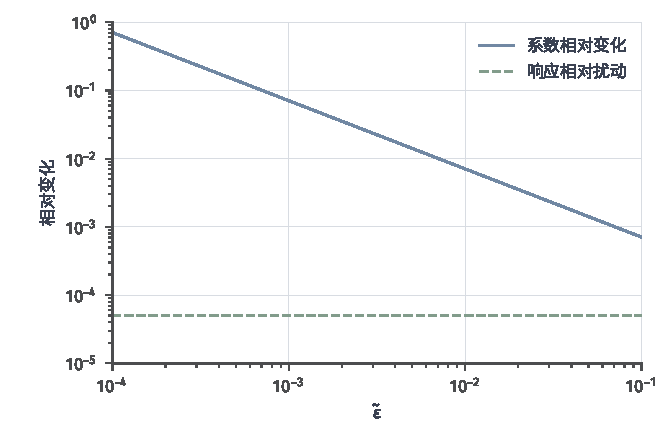
\includegraphics[width=0.92\linewidth]{figures/01-mathematical-preliminaries-upper/03-linear-spaces/matplotlib/matrix-analysis-coefficient-sensitivity/figure.pdf}
 \caption{近平行列的系数分裂：对$\bm A_2=\left[\begin{smallmatrix}1&1\\0&\varepsilon\end{smallmatrix}\right]$固定右端扰动$\eta$，$\varepsilon$越小，两个系数
 沿相反方向偏离$(2,0)$越远，绝对误差随$1/\varepsilon$增长。}
 \label{fig:matrix-analysis-coefficient-sensitivity}
\end{figure}

\paragraph{正规方程的条件数平方}

问题本身的敏感度之外，求解方法也会影响结果。由奇异值分解，$\bm A^\top\bm A$的特征值是$\sigma_i^2$，故满列秩时
\begin{equation}
 \kappa_2(\bm A^\top\bm A)=\kappa_2(\bm A)^2.
 \label{eq:matrix-analysis-normal-equation-condition-square}
\end{equation}
平方的后果在近平行矩阵上看得最清楚。

\begin{example}[形成Gram矩阵时丢失的信息]
\label{ex:ls-gram-rounding-loss}
对示例~\ref{ex:ls-rhs-perturbation-near-parallel}的$\bm A_2$，$\kappa_2(\bm A_2)\approx2/\varepsilon$。
Gram矩阵$\bm A_2^\top\bm A_2=\left[\begin{smallmatrix}1&1\\1&1+\varepsilon^2\end{smallmatrix}\right]$的小特征值约为$\varepsilon^2/2$，条件数约为$4/\varepsilon^2$。
取$\varepsilon=10^{-8}$，则$\varepsilon^2=10^{-16}$已低于双精度的单位舍入$u\approx1.1\times10^{-16}$，
$1+\varepsilon^2$在舍入后就是$1$，存储下来的Gram矩阵成为奇异的$\left[\begin{smallmatrix}1&1\\1&1\end{smallmatrix}\right]$。
而$\bm A_2$本身的条件数约为$2\times10^8$，远未达到$1/u$，它的两列在双精度下仍可区分。
\end{example}

所以形成$\bm A^\top\bm A$这一步就可能把小奇异方向的信息丢掉。这就是第~\ref{sec:ls-qr-method}节的QR方法不形成$\bm A^\top\bm A$的原因：
用Householder反射实现时（第~\ref{sec:ls-orthogonalization-qr}节），它只经过正交变换，不会在问题本身的敏感度之外再把条件数平方。

\paragraph{伪逆的扰动与数值秩}

以上只改右端。矩阵本身改变时，秩是否保持起决定作用。设$\bm A$与$\bm B=\bm A+\bm E$的正奇异值都不小于$s_0>0$。
直接展开右端可验证恒等式
\[
 \bm B^\dagger-\bm A^\dagger
 =-\bm B^\dagger\bm E\bm A^\dagger
 +\bm B^\dagger(\bm I-\bm A\bm A^\dagger)
 -(\bm I-\bm B^\dagger\bm B)\bm A^\dagger .
\]
三项分别估计，其中$\lVert\bm A^\dagger\rVert_2=1/\sigma_r(\bm A)\leq1/s_0$，对$\bm B$同理。
第一项不超过$\lVert\bm B^\dagger\rVert_2\lVert\bm E\rVert_2\lVert\bm A^\dagger\rVert_2\leq\lVert\bm E\rVert_2/s_0^2$。
第二项利用Penrose条件写$\bm B^\dagger=\bm B^\dagger(\bm B\bm B^\dagger)^\top=\bm B^\dagger(\bm B^\dagger)^\top\bm B^\top$；
又因$\bm A^\top(\bm I-\bm A\bm A^\dagger)=\bm0$，有$\bm B^\top(\bm I-\bm A\bm A^\dagger)=\bm E^\top(\bm I-\bm A\bm A^\dagger)$，
所以该项不超过$\lVert\bm B^\dagger\rVert_2^2\lVert\bm E\rVert_2\leq\lVert\bm E\rVert_2/s_0^2$。第三项同理。合起来，
\begin{equation}
 \lVert\bm B^\dagger-\bm A^\dagger\rVert_2
 \leq\frac{3\lVert\bm E\rVert_2}{s_0^2}.
 \label{eq:ch06-pseudoinverse-fixed-rank-perturbation}
\end{equation}
条件“正奇异值都不小于$s_0$”隐含了秩不变。秩改变时没有这样的界。

\begin{example}[反例：秩改变时伪逆不连续]
\label{ex:ls-pinv-discontinuity}
取$\bm A=\operatorname{diag}(1,0)$与$\bm B_\varepsilon=\operatorname{diag}(1,\varepsilon)$，$0<\varepsilon<1$。
二者之差$\lVert\bm B_\varepsilon-\bm A\rVert_2=\varepsilon\to0$，但
\[
 \bm B_\varepsilon^\dagger=\operatorname{diag}(1,1/\varepsilon),\qquad \bm A^\dagger=\operatorname{diag}(1,0),
\]
所以$\lVert\bm B_\varepsilon^\dagger-\bm A^\dagger\rVert_2=1/\varepsilon\to\infty$。
$\bm B_\varepsilon$的秩为$2$，$\bm A$的秩为$1$；两者正奇异值的公共下界只能取$s_0=\varepsilon$，
界~\eqref{eq:ch06-pseudoinverse-fixed-rank-perturbation}给出$3\varepsilon/\varepsilon^2=3/\varepsilon$，同样随$\varepsilon\to0$无界。
\end{example}

这正是上一小节末尾所说的不连续性。

实际数据的秩因而要谨慎对待。第~\ref{chap:linear-analysis}章的奇异值扰动界~\eqref{eq:matrix-analysis-singular-value-perturbation}说明，矩阵改变$\bm E$时每个奇异值的移动不超过$\lVert\bm E\rVert_2$，所以小于数据误差尺度的奇异值与零无法区分：它可能是一个真实但很弱的方向，也可能只是噪声。据此，把大于某个阈值$\tau$的奇异值个数称为\term{数值秩}（numerical rank），$\tau$按数据误差的尺度选取。

综合本小节的分析：无论是方程的解、最小二乘的系数还是伪逆本身，误差放大都来自小奇异值。
它们一方面使增益$1/\sigma_i$很大，另一方面在误差尺度下难以与零区分；形成正规方程之类的计算步骤还会进一步损失精度。
下面分别从数据与计算两方面改进。

\subsubsection{数据计算优化}
\label{sec:ls-truncated-svd-ridge}

前面的分析把误差分成两个来源。一是问题本身：最小范数最小二乘解$\bm A^\dagger\bm b$在右奇异向量$\bm v_i$上的系数是$\bm u_i^\top\bm b/\sigma_i$，
观测误差$\bm e$使它改变$\bm u_i^\top\bm e/\sigma_i$；$\sigma_i$很小时，即使$\bm e$在$\bm u_i$方向上的分量很小，系数的变化也会很大。
二是计算过程：形成$\bm A^\top\bm A$会把条件数平方，有限精度下用Gram--Schmidt算出的$\bm Q$还会逐渐失去正交性。

相应的改进也分两类。要让解对数据误差不那么敏感，只能少用或不用小奇异值方向，这必然改变所求的问题，岭回归和截断SVD分别对应“少用”与“不用”；
要让计算不额外放大误差，则在不改变问题的前提下更稳定地算出QR分解，修正Gram--Schmidt、Householder反射与Givens旋转属于这一类。
下面依次介绍这五种做法。

\paragraph{岭回归}
\label{sec:ls-regularized-ls}

示例~\ref{ex:ls-nearly-collinear-design}中，系数为了拟合上的微小改进而取得很大。若任务希望输入不要太大，
可以在数据项之外加上输入长度的平方惩罚，得到\term{岭回归}（ridge regression）
\begin{equation}
 \min_{\bm x}\ \lVert\bm A\bm x-\bm b\rVert_2^2+\lambda\lVert\bm x\rVert_2^2,
 \qquad \lambda>0.
 \label{eq:ls-ridge-objective}
\end{equation}
参数$\lambda$权衡两项：$\lambda$越大，越倾向于小的输入，拟合误差也越大。

更一般地，惩罚可以作用在希望压小的量$\bm L\bm x$上，$\bm L\in\mathbb R^{p\times d}$，例如相邻分量之差，
得到\term{Tikhonov正则化}（Tikhonov regularization）\scite{math-hansen2008regtools}
\begin{equation}
 \min_{\bm x}\ \lVert\bm A\bm x-\bm b\rVert_2^2+\lambda\lVert\bm L\bm x\rVert_2^2,
 \qquad \lambda>0.
 \label{eq:linear-algebra-general-tikhonov}
\end{equation}
两项都是平方长度，而$\lambda\lVert\bm L\bm x\rVert_2^2=\lVert\sqrt\lambda\,\bm L\bm x-\bm0\rVert_2^2$，
所以可以把两个残差向量上下堆成一个更长的残差向量，写成堆叠矩阵的普通最小二乘，
称为\term{增广最小二乘}（augmented least squares）：
\begin{equation}
 \begin{bmatrix}\bm A\\ \sqrt{\lambda}\,\bm L\end{bmatrix}\bm x
 \approx\begin{bmatrix}\bm b\\ \bm0\end{bmatrix}.
 \label{eq:ls-augmented-system}
\end{equation}
对堆叠矩阵套用正规方程~\eqref{eq:linear-algebra-normal-equations}：堆叠矩阵的转置乘自身是
$\bm A^\top\bm A+\lambda\bm L^\top\bm L$，转置乘堆叠右端是$\bm A^\top\bm b$，于是
\begin{equation}
 (\bm A^\top\bm A+\lambda\bm L^\top\bm L)\hat{\bm x}=\bm A^\top\bm b.
 \label{eq:ls-tikhonov-normal}
\end{equation}
它是普通最小二乘，存在性自动成立。由~\eqref{eq:ls-normal-kernel}，系数矩阵的零空间就是堆叠矩阵的零空间，
即同时满足$\bm A\bm x=\bm0$与$\bm L\bm x=\bm0$的向量，所以解唯一当且仅当
\begin{equation}
 \ker\bm A\cap\ker\bm L=\{\bm0\}.
 \label{eq:linear-algebra-tikhonov-common-nullspace}
\end{equation}
$\bm L=\bm I$时条件自动成立，岭回归对任意$\bm A$都有唯一解。其他惩罚则未必。

\begin{example}[反例：惩罚无法确定的方向]
\label{ex:ls-tikhonov-common-nullspace}
取$\bm A=\bm L=[\,1\ -1\,]$。两者的零空间都是$\operatorname{span}\{(1,1)^\top\}$，条件~\eqref{eq:linear-algebra-tikhonov-common-nullspace}不成立。
对任何解$\hat{\bm x}$和任何$t\in\mathbb R$，$\hat{\bm x}+t(1,1)^\top$的数据项与惩罚项都不变，因而也是解。
所以无论$\lambda$多大，都不能确定两个分量的共同水平。
\end{example}

权重与惩罚也可以同时使用，目标
$(\bm A\bm x-\bm b)^\top\bm M(\bm A\bm x-\bm b)+\lambda\lVert\bm L\bm x\rVert_2^2$的正规方程为
\begin{equation}
 (\bm A^\top\bm M\bm A+\lambda\bm L^\top\bm L)\hat{\bm x}=\bm A^\top\bm M\bm b,
 \label{eq:ls-general-normal-equations}
\end{equation}
$\bm M$正定、$\lambda>0$时，解唯一的条件仍是~\eqref{eq:linear-algebra-tikhonov-common-nullspace}。
要注意，加惩罚改变的是问题本身：选择$\lambda$是在重新设定任务，而不是让原方程“算得出来”的数值技巧。

$\lambda$怎样影响解，可以在奇异值坐标中读出。岭回归的正规方程是$(\bm A^\top\bm A+\lambda\bm I)\bm x=\bm A^\top\bm b$。在右奇异向量坐标$c_i=\bm v_i^\top\bm x$中，
$\bm A^\top\bm A$与$\bm I$同时成为对角矩阵，方程按方向分开：$i\leq r$时$(\sigma_i^2+\lambda)c_i=\sigma_i\,\bm u_i^\top\bm b$，
$i>r$时$\lambda c_i=0$，故$c_i=0$。于是
\begin{equation}
 \hat{\bm x}_\lambda=\sum_{i=1}^r\frac{\sigma_i}{\sigma_i^2+\lambda}\,(\bm u_i^\top\bm b)\,\bm v_i
 =\sum_{i=1}^r f_i\,\frac{\bm u_i^\top\bm b}{\sigma_i}\,\bm v_i,
 \qquad f_i=\frac{\sigma_i^2}{\sigma_i^2+\lambda}.
 \label{eq:matrix-analysis-ridge-filter-factor}
\end{equation}
前一种写法说明，岭回归把伪逆中的增益$1/\sigma_i$换成了$\sigma_i/(\sigma_i^2+\lambda)$。由$\sigma_i^2+\lambda\geq2\sigma_i\sqrt\lambda$，
新的增益不超过$1/(2\sqrt\lambda)$，不再随$\sigma_i\to0$而爆炸。

后一种写法把它与最小范数解比较：每个方向多乘了一个介于$0$与$1$之间的\term{滤波因子}（filter factor）$f_i$。
$\sigma_i^2\gg\lambda$时$f_i\approx1$，该方向几乎不受影响；$\sigma_i^2\ll\lambda$时$f_i\approx\sigma_i^2/\lambda$，该方向被压低，增益约为$\sigma_i/\lambda$；
$\sigma_i^2=\lambda$处$f_i$恰为$1/2$。代价是大奇异值方向也被轻微压缩，$f_i$总小于$1$。下面在近共线设计上看两个$\lambda$的效果。

\begin{example}[近共线设计上的岭回归]
\label{ex:ls-ridge-nearly-collinear}
沿用示例~\ref{ex:ls-nearly-collinear-design}的$\bm X_\varepsilon$与$\bm y$，取$\varepsilon=0.01$、$\delta=0.1$。
直接计算可得两个奇异值约为$\sigma_1\approx2.449$、$\sigma_2\approx0.0100$，
对应的右奇异向量近似为$(1,1)^\top/\sqrt2$与$(1,-1)^\top/\sqrt2$。精确最小二乘解是$(-9,10)^\top$，残差为零；
它的大系数全部来自第二个方向，该方向的系数$\bm u_2^\top\bm y/\sigma_2$的绝对值约为$0.134/0.0100\approx13.4$。
按式~\eqref{eq:matrix-analysis-ridge-filter-factor}计算两个$\lambda$下的结果：
\[
 \begin{array}{cccc}
  \lambda & f_2 & \hat{\bm x}_\lambda & \lVert\bm X_\varepsilon\hat{\bm x}_\lambda-\bm y\rVert_2\\[2pt]
  10^{-4} & \approx0.50 & \approx(-4.25,\,5.25)^\top & \approx0.067\\
  10^{-2} & \approx0.0099 & \approx(0.41,\,0.59)^\top & \approx0.133
 \end{array}
\]
$\lambda=10^{-4}\approx\sigma_2^2$时，第二个方向保留一半；$\lambda=10^{-2}$时，第二个方向几乎被去掉。
第一个方向的因子$f_1$在两种情形下都大于$0.998$。所以随着$\lambda$增大，解从精确拟合的大系数逐渐移向两个系数平分共同作用的解，
代价是残差增大。
\end{example}

计算岭回归不必作奇异值分解，上面的滤波因子只用于解释$\lambda$的作用。正规方程$(\bm A^\top\bm A+\lambda\bm I)\hat{\bm x}=\bm A^\top\bm b$的系数矩阵对任意$\bm A$都正定，
可以用Cholesky分解；更可靠的做法是对堆叠矩阵~\eqref{eq:ls-augmented-system}作QR分解，避免形成$\bm A^\top\bm A$。
一般的Tikhonov惩罚（$\bm L\neq\bm I$）不能由$\bm A$一个矩阵的奇异值分解按方向分开，但同样可以用堆叠矩阵的QR分解求解。

核验时要回到原目标，分别报告数据项$\lVert\bm A\hat{\bm x}-\bm b\rVert_2^2$（加权时为$\bm M$加权长度）、惩罚项$\lambda\lVert\bm L\hat{\bm x}\rVert_2^2$
以及正规方程~\eqref{eq:ls-general-normal-equations}的残差，不能只报告堆叠问题的残差。

\paragraph{修正Gram--Schmidt}

用QR分解解最小二乘（第~\ref{sec:ls-qr-method}节），以及上面用堆叠矩阵解岭回归，都要先算出QR分解。
第~\ref{chap:linear-representation}章用Gram--Schmidt正交化构造它，那里假定精确算术：
式~\eqref{eq:ls-gram-schmidt}一次性减去$\bm a_j$在全部旧方向上的分量，每个系数都用原始的$\bm a_j$计算。

\term{修正Gram--Schmidt}（modified Gram--Schmidt）改为逐个扣除：先令$\bm u\leftarrow\bm a_j$，对$i=1,\ldots,j-1$依次计算$r_{i,j}=\langle\bm u,\bm q_i\rangle$并更新$\bm u\leftarrow\bm u-r_{i,j}\bm q_i$，最后归一化。
精确算术中两种做法给出同样的结果：扣除第$i$个方向时，此前已减去的都是$\bm q_1,\ldots,\bm q_{i-1}$的倍数，它们与$\bm q_i$正交，所以$\langle\bm u,\bm q_i\rangle=\langle\bm a_j,\bm q_i\rangle$。

有限精度下，修正的做法每次都从已经扣除过的最新残差出发，算出的$\bm q_j$之间正交性的损失通常更小；
它的损失大致与$\kappa_2(\bm A)$乘单位舍入$u$同量级，原始做法则可能严重得多\scite{math-golub2013matrix}。
列之间越接近线性相关，扣除后剩下的$\bm u_j$越短，舍入误差在其中所占的比例越大，两种做法的差别也越明显。

同样的原因使列相关时的处理不能照搬精确算术：有限精度下$\bm u_j$很少恰好为零，判断“没有新方向”时要把$\lVert\bm u_j\rVert$与一个容限比较，
这正是第~\ref{sec:ls-ordinary-ls-sensitivity}节的数值秩问题。修正Gram--Schmidt的正交性损失仍随条件数增长；
需要$\bm Q$在工作精度下正交时，改用后面的Householder反射。

\paragraph{截断SVD}

岭回归按滤波因子连续地压低小奇异值方向。更直接的做法是只在前$k$个奇异方向上反演，丢弃其余方向：
\[
 \bm x_k=\sum_{i=1}^k\frac{\bm u_i^\top\bm b}{\sigma_i}\,\bm v_i,\qquad 1\leq k\leq r ,
\]
相当于滤波因子只取$1$（$i\leq k$）或$0$（$i>k$）。$k=r$时它就是$\bm A^\dagger\bm b$；$k<r$时，它恰是把$\bm A$换成第~\ref{sec:ls-svd}节的截断SVD$\bm A_k=\sum_{i\leq k}\sigma_i\bm u_i\bm v_i^\top$
（式~\eqref{eq:matrix-analysis-truncated-svd}）后，所得问题的最小范数最小二乘解，即$\bm x_k=\bm A_k^\dagger\bm b$。
由Eckart--Young--Mirsky定理~\ref{thm:matrix-analysis-best-low-rank}，$\bm A_k$是离$\bm A$最近的秩$k$矩阵，
所以截断SVD解相当于先用最接近的低秩矩阵代替$\bm A$，再精确地解代替后的问题。

收益与代价都可以从坐标中直接读出。收益是放大倍数受控：观测误差对$\bm x_k$的影响至多被放大$1/\sigma_k$倍，
而不是$1/\sigma_r$倍。代价是残差增加：被丢弃方向上的观测分量不再被拟合，平方残差比原最小二乘问题多出
$\sum_{i=k+1}^r(\bm u_i^\top\bm b)^2$。若这些分量主要来自噪声，丢弃它们正是所求；若其中含有真实信号，信号也一并丢失。
$k$取多大，取决于哪些奇异值可以与零区分：取$k$为数值秩，就是只在可信的方向上反演。下面仍用近共线设计说明。

\begin{example}[近共线设计上的截断SVD]
\label{ex:ls-tsvd-nearly-collinear}
沿用示例~\ref{ex:ls-ridge-nearly-collinear}的数据与奇异值分解，取$k=1$，只保留第一个奇异方向：
\[
 \bm x_1=\frac{\bm u_1^\top\bm y}{\sigma_1}\,\bm v_1\approx(0.50,\,0.50)^\top .
\]
两个系数平分共同的作用。残差长度约为$0.134$，即被丢弃的分量$|\bm u_2^\top\bm y|$，接近响应中$\delta\bm q$部分的长度$\delta\sqrt2\approx0.141$。
$\lambda=10^{-2}$时的岭回归解$(0.41,0.59)^\top$已经接近它。
\end{example}

截断以后，拟合不再精确，但系数不再随$\delta/\varepsilon$而爆炸。

截断SVD需要奇异值分解，适合规模不大、或需要逐个检查奇异值的情形。

$k$与$\lambda$都不是由方程本身确定的量。它们决定在多大程度上用拟合误差换取解的稳定，
应当按任务对两者的要求、以及数据误差的尺度来选择；常见的办法是比较不同参数下残差与解的大小\scite{math-hansen2008regtools}，
或在留出的数据上检验预测效果。无论用哪种办法，报告结果时都应说明所用的$k$或$\lambda$，因为它们改变的是所解的问题。

\paragraph{Householder反射}
\label{sec:ls-orthogonalization-qr}

修正Gram--Schmidt仍从列出发构造$\bm Q$，列越接近线性相关，正交性损失越大，而这恰是最需要QR的情形。
稠密计算中更常用的做法反过来：用一串正交矩阵从左边作用于$\bm A$，逐列把主对角线以下的元素消成零，最后剩下上三角的$\bm R$。
正交矩阵保持长度，这样的消元不会放大误差，各步正交矩阵的乘积自然是正交的。
完成这一步的基本工具是\term{Householder反射}，它一次消去一列中主对角线以下的全部元素。

对非零向量$\bm a$，要找一个正交矩阵把它变成$\bm e_1$的倍数。由于正交变换保持长度，目标只能是$\pm\lVert\bm a\rVert_2\bm e_1$。
取$s=1$（若$a_1\geq0$）或$s=-1$（若$a_1<0$），令
\begin{equation}
 \bm v=\bm a+s\lVert\bm a\rVert_2\bm e_1,\qquad
 \bm H=\bm I-2\frac{\bm v\bm v^\top}{\bm v^\top\bm v}.
 \label{eq:ls-householder}
\end{equation}
$\bm H$把$\bm v$方向的分量变号，与$\bm v$正交的分量保持不变，即关于以$\bm v$为法向的超平面作镜面反射；
它对称，且$\bm H^\top\bm H=\bm H^2=\bm I$，反射两次回到原处。

下面验证它把$\bm a$送到$\bm e_1$方向。记$\alpha=\lVert\bm a\rVert_2$，则
$\bm v^\top\bm a=\alpha^2+s\alpha a_1$，$\bm v^\top\bm v=\alpha^2+2s\alpha a_1+\alpha^2=2\bm v^\top\bm a$，于是
\[
 \bm H\bm a=\bm a-2\frac{\bm v^\top\bm a}{\bm v^\top\bm v}\bm v=\bm a-\bm v=-s\alpha\bm e_1 .
\]
符号$s$取与$a_1$相同，是为了让$\bm v$的首元素$a_1+s\alpha$是两个同号数相加，避免两个相近的数相减而丢失有效数字。
应用$\bm H$时只需保存$\bm v$，计算$\bm H\bm x=\bm x-2\bm v(\bm v^\top\bm x)/(\bm v^\top\bm v)$，不必形成整个矩阵。

\begin{example}[二维向量的Householder反射]
\label{ex:ls-householder-two-dim}
取$\bm a=(3,4)^\top$。$a_1>0$，取$s=1$；$\alpha=5$，$\bm v=\bm a+5\bm e_1=(8,4)^\top$，$\bm v^\top\bm v=80$。于是
\[
 \bm H=\bm I-\frac{2}{80}\bm v\bm v^\top
 =\bm I-\frac1{40}\begin{bmatrix}64&32\\32&16\end{bmatrix}
 =\begin{bmatrix}-3/5&-4/5\\-4/5&3/5\end{bmatrix},
\]
$\bm H\bm a=(-5,0)^\top$，与$-s\alpha\bm e_1=-5\bm e_1$一致。
\end{example}

对矩阵做QR时，第$k$步对第$k$列从第$k$个元素往下的部分构造反射，
只作用于尚未处理的右下子块。$d$步之后，$\bm H_d\cdots\bm H_1\bm A=\left[\begin{smallmatrix}\bm R\\\bm0\end{smallmatrix}\right]$，
各反射的乘积的转置就是完全QR分解中的$[\bm Q_1\;\bm Q_2]$；
$\bm R$的对角元可能为负，把相应的行与$\bm Q_1$的列同时变号即可化为对角元为正的形式。

稠密$m\times d$矩阵的Householder QR约需$2md^2-2d^3/3$次浮点运算。$\bm Q$不必显式形成，
保存各步的反射向量即可；求解最小二乘时，把同样的反射依次作用于$\bm b$就得到$\bm c_1$与$\bm c_2$，
多个右端复用全部反射与$\bm R$。岭回归对堆叠矩阵~\eqref{eq:ls-augmented-system}作同样的分解即可，
不必形成$\bm A^\top\bm A+\lambda\bm L^\top\bm L$。

秩亏或接近秩亏时，要先把列重新排序。带列主元的QR在每一步选剩余部分中最长的一列先处理，
使接近零的对角元集中在$\bm R$的尾部，从而暴露数值秩，阈值按数据误差的尺度选取，这比计算奇异值分解便宜。
确定秩$r$后，只用前$r$个主元列回代，其余未知量取零，得到一个基本解。它使目标达到最小，是合法的最小二乘解，
但一般不是最小范数解，正如第~\ref{sec:ls-select-among-solutions}节中自由变量取零得到的特解一般不是最小范数解。

\paragraph{Givens旋转}

\term{Givens旋转}一次只消去一个元素。它在第$i$、$j$两个坐标构成的平面内作旋转，其余坐标不变；
在这两个坐标上的作用是
\begin{equation}
 \begin{bmatrix}a_i\\a_j\end{bmatrix}\mapsto
 \begin{bmatrix}c&s\\-s&c\end{bmatrix}
 \begin{bmatrix}a_i\\a_j\end{bmatrix},
 \qquad c^2+s^2=1.
 \label{eq:ls-givens}
\end{equation}
这里的$c$、$s$是旋转角的余弦与正弦，与Householder反射中的符号$s$无关。
完整的矩阵$\bm G(i,j)$是在单位矩阵的$(i,i),(i,j),(j,i),(j,j)$四个位置放上$c,s,-s,c$。
为了消去$a_j$，取$r=\sqrt{a_i^2+a_j^2}$，$c=a_i/r$、$s=a_j/r$，则新分量为
$(ca_i+sa_j,\,-sa_i+ca_j)=(r,0)$。$r=0$时两个分量本已为零，无需旋转。

\begin{example}[二维向量的Givens旋转]
\label{ex:ls-givens-two-dim}
取$(a_i,a_j)=(3,4)$。$r=\sqrt{9+16}=5$，$c=3/5$、$s=4/5$，旋转后
\[
 ca_i+sa_j=\frac95+\frac{16}5=5,\qquad -sa_i+ca_j=-\frac{12}5+\frac{12}5=0 ,
\]
第二个分量被消去，长度$5$全部转到第一个分量上。
\end{example}

Givens每次只改动两行，适合稀疏或带状矩阵，也适合在最小二乘中新增一条观测时逐步更新已有的QR；
对稠密矩阵，它消去同样多的元素需要更多运算，不如Householder。
图~\ref{fig:ls-givens-householder-elimination}把两种变换并置。图中的反射取另一种符号，
把向量映到$(r,0)^\top$而不是$(-r,0)^\top$，精确算术中两种选择都可以。

\begin{figure*}[htbp]
  \centering
  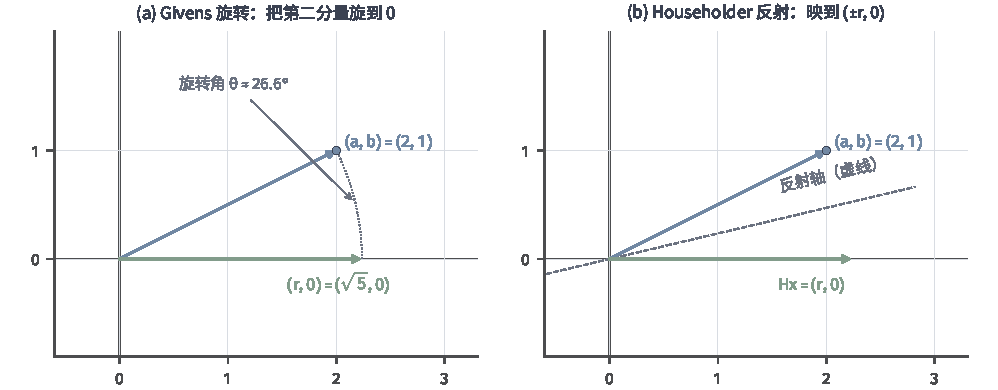
\includegraphics[width=168.998mm]{figures/01-mathematical-preliminaries-upper/03-linear-spaces/matplotlib/ls-givens-householder-elimination/ls-givens-householder-elimination.pdf}
  \caption{两种初等正交消元。左：Givens旋转把$(a,b)=(2,1)^\top$沿圆弧旋到
  $(r,0)^\top$，$r=\sqrt5$，旋转角$\theta=\arctan(1/2)$；右：Householder反射沿角平分线
  把同一向量映到$(r,0)^\top$。两者都是正交变换，保持长度，区别在旋转（行列式$+1$）与
  反射（对称正交）。解析式教学构造。}
  \label{fig:ls-givens-householder-elimination}
\end{figure*}

至此，本节对线性方程的讨论告一段落：用秩判别解的情况；唯一解由直接法算出；无穷多解是特解加零空间，
可按最小范数挑出一个；无解时改求最小二乘；伪逆把三种情况统一为$\bm A^\dagger\bm b$；
数据有误差时，条件数刻画解的放大，小奇异值是放大的根源。岭回归与截断SVD以改变问题为代价换取稳定，
修正Gram--Schmidt、Householder反射与Givens旋转则在不改变问题的前提下减少计算带来的误差。

% 矩阵方程：西尔维斯特（Sylvester）方程AX+XB=C（线性算子、可逆性、求解：一般情况与可对角情况）；
% 李雅普诺夫（Lyapunov）方程AX+XA^T=Q与离散型X-A^TXA=Q（可解性与对称性、求解、正定性与离散级数解）；本章小结

\section{西尔维斯特方程}
\label{sec:ls-matrix-equations}
\label{sec:linear-algebra-matrix-equations}

上一节的未知量是向量。本节和下一节的未知量本身是一张矩阵，已知矩阵从左边、右边或两边乘在它上面，
这样的方程称为\term{矩阵方程}（matrix equation）。本节的主角是西尔维斯特（Sylvester）方程：
未知矩阵分别受到左乘与右乘，两种作用相加。我们回答三个问题：方程表达什么，
何时有解、何时唯一，以及怎样求解。

\subsection{方程与线性算子}
\label{sec:ls-matrix-equation-types}

最简单的矩阵方程只从一侧作用。单侧方程$\bm A\bm X=\bm C$就是上一节的多右端方程：左乘$\bm A$对$\bm X$的每一列
做同一个线性变换。类似地，右乘对每一行做同一个线性变换。双侧方程$\bm A\bm X\bm B=\bm C$同时受两侧约束。
本节的重点是两侧作用相加的情形。

\begin{definition}[Sylvester方程]
\label{def:matrix-analysis-sylvester-equation}
给定$\bm A\in\mathbb R^{m\times m}$、$\bm B\in\mathbb R^{n\times n}$、$\bm C\in\mathbb R^{m\times n}$，
求$\bm X\in\mathbb R^{m\times n}$使
\[
 \bm A\bm X+\bm X\bm B=\bm C .
\]
这一方程称为\term{Sylvester方程}（Sylvester equation）。
\end{definition}

方程的左边是$\bm X$的函数$\mathcal L(\bm X)=\bm A\bm X+\bm X\bm B$，它把$\mathbb R^{m\times n}$映到自身。
由矩阵乘法的分配律，$\mathcal L(\alpha\bm X_1+\beta\bm X_2)=\alpha\mathcal L(\bm X_1)+\beta\mathcal L(\bm X_2)$，
所以$\mathcal L$是$mn$维空间$\mathbb R^{m\times n}$上的线性算子，Sylvester方程就是线性方程$\mathcal L(\bm X)=\bm C$。
上一节关于线性方程的结论因此全部适用。特别地，$\mathcal L$把一个空间映到同维的自身，
由秩零度定理，它对每个$\bm C$都有唯一解，当且仅当齐次方程$\mathcal L(\bm X)=\bm0$只有零解。

\paragraph{向量化与Kronecker表示}

为了真正套用上一节的工具，可以把矩阵拉直成向量。第~\ref{sec:ls-kronecker-products}节的向量化恒等式
$\operatorname{vec}(\bm A\bm X\bm B)=(\bm B^\top\otimes\bm A)\operatorname{vec}\bm X$
把矩阵乘积写成Kronecker积作用于向量。对$\bm A\bm X=\bm A\bm X\bm I_n$取$\bm B=\bm I_n$，
对$\bm X\bm B=\bm I_m\bm X\bm B$取$\bm A=\bm I_m$，两式相加，Sylvester方程化为
\begin{equation}
 (\bm I_n\otimes\bm A+\bm B^\top\otimes\bm I_m)\operatorname{vec}\bm X
 =\operatorname{vec}\bm C.
 \label{eq:ls-sylvester-vectorized}
\end{equation}
这是一个$mn$阶的普通线性方程。双侧方程同理化为$(\bm B^\top\otimes\bm A)\operatorname{vec}\bm X=\operatorname{vec}\bm C$。
于是第~\ref{sec:ls-solution-cases}节的相容性判据与解集结构都可以直接用在矩阵方程上。

\subsection{存在性与唯一性}
\label{sec:ls-matrix-equation-existence}

单侧和双侧方程可以直接沿用列空间的判据。单侧方程$\bm A\bm X=\bm C$相容，当且仅当$\bm C$的每一列都在$\operatorname{range}\bm A$中，
即$\operatorname{rank}[\bm A\ \bm C]=\operatorname{rank}\bm A$。双侧方程$\bm A\bm X\bm B=\bm C$的左边，每一列都是$\bm A$的列的组合，
每一行都是$\bm B$的行的组合，所以相容的必要条件是$\operatorname{range}\bm C\subseteq\operatorname{range}\bm A$
且$\operatorname{range}\bm C^\top\subseteq\operatorname{range}\bm B^\top$；完整的判据是向量化方程的增广秩条件。
$\bm A,\bm B$都可逆时，两侧分别乘逆，得唯一解$\bm X=\bm A^{-1}\bm C\bm B^{-1}$。任一侧秩亏时，不能写出这个公式：
方程可能无解，有解时解还可以沿该侧的零空间变动，不唯一。

Sylvester方程的两项相加，情况不同：可解性不取决于$\bm A$、$\bm B$各自是否可逆，而取决于二者的特征值如何搭配。
下面先从对角情形看出这一点，再给出一般结论。

\paragraph{对角情形}

设$\bm A$与$\bm B$都是对角矩阵，对角元分别为$a_{i,i}$与$b_{j,j}$。$\bm A\bm X$把$\bm X$的第$i$行乘以$a_{i,i}$，
$\bm X\bm B$把第$j$列乘以$b_{j,j}$，所以$(\bm A\bm X+\bm X\bm B)_{i,j}=(a_{i,i}+b_{j,j})x_{i,j}$。
方程按元素分解成$mn$个互不相关的标量方程$(a_{i,i}+b_{j,j})x_{i,j}=c_{i,j}$，
只要每个分母非零，就有唯一解
\begin{equation}
 x_{i,j}=\frac{c_{i,j}}{a_{i,i}+b_{j,j}}.
 \label{eq:ls-sylvester-diagonal-closed-form}
\end{equation}
若某一对满足$a_{i,i}+b_{j,j}=0$，该位置的方程退化为$0\cdot x_{i,j}=c_{i,j}$：$c_{i,j}\neq0$时无解，$c_{i,j}=0$时该元素可任意取值。

对角元就是特征值，所以对角情形下，方程对每个$\bm C$唯一可解的条件是：$\bm A$的任一特征值与$\bm B$的任一特征值之和都不为零，
也就是$\bm A$的特征值与$-\bm B$的特征值互不相同。这个条件与$\bm A$、$\bm B$各自是否可逆无关，两个方向都有例子。

\begin{example}[反例：可解性不取决于各自可逆]
\label{ex:ls-sylvester-invertibility-irrelevant}
取$\bm A=\bm0\in\mathbb R^{m\times m}$、$\bm B=\bm I_n$。$\bm A$不可逆，但方程化为$\bm X=\bm C$，对每个$\bm C$唯一可解；
这里$\bm A$的特征值只有$0$，$-\bm B$的特征值只有$-1$，二者分离。

反过来，取$m=n=1$、$\bm A=2$、$\bm B=-2$，两者都可逆，方程却化为$(2-2)x=c$，即$0\cdot x=c$：
$c\neq0$时无解，$c=0$时任意$x$都是解。这里$2+(-2)=0$，分离条件不成立。
\end{example}

图~\ref{fig:ls-sylvester-separation}把这一分离条件画在实轴上。

\begin{figure}[htbp]
  \centering
  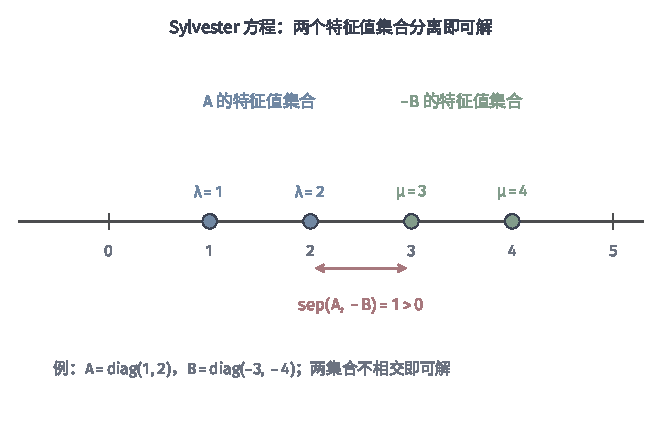
\includegraphics[width=112mm]{figures/01-mathematical-preliminaries-upper/03-linear-spaces/matplotlib/ls-sylvester-separation/ls-sylvester-separation.pdf}
  \caption{Sylvester方程$\bm A\bm X+\bm X\bm B=\bm C$的特征值分离条件。
  $\bm A=\operatorname{diag}(1,2)$的特征值$\{1,2\}$与$-\bm B$（$\bm B=\operatorname{diag}(-3,-4)$）
  的特征值$\{3,4\}$分居实轴两侧，最近一对间距$|2-3|=1>0$，
  两集合不相交，故对任意$\bm C$有唯一解。只用实轴，不引入复数对象。}
  \label{fig:ls-sylvester-separation}
\end{figure}

\paragraph{Sylvester算子的可逆性}

一般情形的结论与对角情形相同。Sylvester算子$\mathcal L(\bm X)=\bm A\bm X+\bm X\bm B$可逆，当且仅当
\begin{equation}
 \lambda_i(\bm A)+\lambda_j(\bm B)\neq0
 \quad\text{对所有 }i,j,
 \qquad\text{即}\qquad
 \operatorname{spec}(\bm A)\cap\operatorname{spec}(-\bm B)=\varnothing,
 \label{eq:ch06-sylvester-spectral-separation}
\end{equation}
其中$\operatorname{spec}$表示全体特征值，包括复特征值。实矩阵的特征值可能是复数（第~\ref{sec:ls-general-square-spectrum}节），所以条件要对全体特征值检查。

证明中会用到复特征向量。这样做是允许的：$\mathcal L$可逆等价于Kronecker矩阵~\eqref{eq:ls-sylvester-vectorized}的行列式非零，
而行列式不论在实数域还是复数域中计算都是同一个数，所以在复数域中证明齐次方程只有零解，也就证明了实算子可逆。

必要性。设条件不成立，即有$\bm A\bm u=\lambda\bm u$（$\bm u\neq\bm0$），且$-\lambda$是$\bm B$的特征值。
$\bm B^\top$与$\bm B$的特征多项式相同（$\det(\bm B^\top-\mu\bm I)=\det(\bm B-\mu\bm I)$），
所以存在$\bm w\neq\bm0$使$\bm B^\top\bm w=-\lambda\bm w$，即$\bm w^\top\bm B=-\lambda\bm w^\top$。
取$\bm X=\bm u\bm w^\top$，它不是零矩阵，而
\[
 \bm A\bm X+\bm X\bm B=(\bm A\bm u)\bm w^\top+\bm u(\bm w^\top\bm B)
 =\lambda\bm u\bm w^\top-\lambda\bm u\bm w^\top=\bm0 .
\]
齐次方程有非零解，算子不可逆。

充分性。设条件成立，且$\mathcal L(\bm X)=\bm0$，要证$\bm X=\bm0$。思路是找一个多项式$q$，
使$q(\bm A)=\bm0$而$q(-\bm B)$可逆，再利用二者与$\bm X$的关系。

第一步，把$\bm X$在两侧之间“搬运”。由$\bm A\bm X=\bm X(-\bm B)$，
得$\bm A^2\bm X=\bm A\bm X(-\bm B)=\bm X(-\bm B)^2$，归纳得$\bm A^k\bm X=\bm X(-\bm B)^k$；
对各次幂作线性组合，对任意多项式$q$有$q(\bm A)\bm X=\bm X\,q(-\bm B)$。

第二步，取$q$为$\bm A$的特征多项式$p_{\bm A}(z)=\det(z\bm I-\bm A)$。由Cayley--Hamilton定理~\ref{thm:ls-cayley-hamilton}，
$p_{\bm A}(\bm A)=\bm0$。在复数域中分解$p_{\bm A}(z)=\prod_k(z-\lambda_k)$，其中$\lambda_k$取遍$\bm A$的全部特征值，则
$p_{\bm A}(-\bm B)=\prod_k(-\bm B-\lambda_k\bm I)$。由条件~\eqref{eq:ch06-sylvester-spectral-separation}，
每个$\lambda_k$都不是$-\bm B$的特征值，所以每个因子$-\bm B-\lambda_k\bm I$都可逆，$p_{\bm A}(-\bm B)$作为可逆矩阵的乘积也可逆。

合起来，$\bm X\,p_{\bm A}(-\bm B)=p_{\bm A}(\bm A)\bm X=\bm0$，右乘$p_{\bm A}(-\bm B)^{-1}$得$\bm X=\bm0$。齐次方程只有零解，算子可逆。

至此，Sylvester方程的存在性与唯一性完全由$\bm A$与$-\bm B$的特征值是否分离决定。
条件不成立时，方程对有些右端无解、对另一些右端有无穷多解，齐次解$\bm u\bm w^\top$给出了解不唯一的方向。

\subsection{求解方法}
\label{sec:ls-matrix-equation-solve}

求解方法按$\bm A$、$\bm B$的结构分两种情况。一般情况下，方程可以化为普通线性方程直接求解，
但规模大时要用实Schur形把它约化成准三角形再逐块回代；$\bm A$、$\bm B$可对角化时，换到特征向量坐标后方程按元素分开，直接写出解。

\subsubsection{一般情况}
\label{sec:ls-one-sided-two-sided}

\paragraph{向量化直接求解}

最直接的做法是形成系数矩阵~\eqref{eq:ls-sylvester-vectorized}，用第~\ref{sec:ls-direct-methods}节的LU分解求解。
小规模问题这样做是可靠的，但系数矩阵有$(mn)^2$个元素，稠密LU约需$2(mn)^3/3$次运算；
$m=n=100$时系数矩阵已有$10^8$个元素。所以要尽量利用方程的结构，避免形成这个大矩阵。

单侧和双侧方程很容易做到。$\bm A\bm X=\bm C$是同一系数矩阵的多右端问题，对$\bm A$分解一次即可逐列复用。
双侧方程在$\bm A,\bm B$可逆时，先解$\bm A\bm Y=\bm C$，再解$\bm X\bm B=\bm Y$（即$\bm B^\top\bm X^\top=\bm Y^\top$），
也不形成Kronecker矩阵。双侧方程不相容时，可以改求$\min_{\bm X}\lVert\bm A\bm X\bm B-\bm C\rVert_{\mathrm F}^2$，
它是系数矩阵为$\bm B^\top\otimes\bm A$的最小二乘问题，由第~\ref{sec:ls-least-squares}节的方法求解。
Sylvester方程的两项相加，不能这样逐侧处理，下面借助$\bm A$、$\bm B$的正交相似变换。

\paragraph{实Schur约化}
\label{sec:ls-sylvester-schur}

正交变换不放大误差，而且由第~\ref{sec:ls-general-square-spectrum}节的实Schur形（定理~\ref{thm:ls-real-schur}），
任何实方阵都可以用正交相似化为接近三角的形状：$\bm A=\bm Q\bm T\bm Q^\top$，
$\bm Q$正交，$\bm T$是实准上三角矩阵，即对角线上是$1\times1$块（实特征值）或$2\times2$块（一对共轭复特征值），
对角块以下全为零。

分别取$\bm A=\bm Q\bm T\bm Q^\top$、$\bm B=\bm U\bm S\bm U^\top$，方程两边左乘$\bm Q^\top$、右乘$\bm U$，
利用$\bm Q^\top\bm A=\bm T\bm Q^\top$与$\bm B\bm U=\bm U\bm S$，并记$\bm Y=\bm Q^\top\bm X\bm U$、$\bm D=\bm Q^\top\bm C\bm U$，方程化为
\begin{equation}
 \bm T\bm Y+\bm Y\bm S=\bm D.
 \label{eq:ls-sylvester-transformed}
\end{equation}
正交相似不改变特征值，所以可逆条件不变；正交变换也不改变Frobenius范数，所以新坐标下的残差大小与原坐标相同。

\paragraph{准三角块上的逐块回代}

$\bm T$、$\bm S$不是对角的，方程不能按元素完全分开，但三角结构允许逐块依次求解，正如上三角方程可以回代。
按$\bm T$、$\bm S$的对角块把$\bm Y$、$\bm D$分块，比较第$(i,j)$块：
$(\bm T\bm Y)_{i,j}=\sum_k\bm T_{i,k}\bm Y_{k,j}$中只有$k\geq i$的项非零，
$(\bm Y\bm S)_{i,j}=\sum_\ell\bm Y_{i,\ell}\bm S_{\ell,j}$中只有$\ell\leq j$的项非零。
把含$\bm Y_{i,j}$的两项留在左边，其余移到右边：
\begin{equation}
 \bm T_{i,i}\bm Y_{i,j}+\bm Y_{i,j}\bm S_{j,j}
 =\bm D_{i,j}-\sum_{k>i}\bm T_{i,k}\bm Y_{k,j}
          -\sum_{\ell<j}\bm Y_{i,\ell}\bm S_{\ell,j}.
 \label{eq:ls-sylvester-block-recurrence}
\end{equation}
右边只用到同一列中更靠下的块$\bm Y_{k,j}$（$k>i$）和同一行中更靠左的块$\bm Y_{i,\ell}$（$\ell<j$）。
因此按列从左到右、每列从下到上的次序计算，每次右边需要的块都已求出。左边是一个小的Sylvester方程：
两个对角块都是$1\times1$时，它就是标量方程，直接除以$t_{i,i}+s_{j,j}$；含$2\times2$块时，它至多含$4$个未知量，
向量化后系数矩阵为$\bm I\otimes\bm T_{i,i}+\bm S_{j,j}^\top\otimes\bm I$。小块的特征值是$\bm A$、$\bm B$特征值的一部分，
由谱分离条件，每个小方程都唯一可解。

全部块求出后，由$\bm X=\bm Q\bm Y\bm U^\top$恢复原坐标，并在原坐标中计算残差$\bm A\bm X+\bm X\bm B-\bm C$。这一方法称为Bartels--Stewart算法。
两次实Schur约化的代价为$O(m^3+n^3)$，逐块回代的代价为$O(mn(m+n))$，远小于向量化直接求解的$O(m^3n^3)$；
约化只做一次，多个右端$\bm C$可以复用。

\subsubsection{可对角情况}
\label{sec:ls-sylvester-diagonalizable}

若$\bm A$、$\bm B$可以对角化，逐块回代可以省去：换到特征向量坐标后，问题就是对角情形，有闭式解~\eqref{eq:ls-sylvester-diagonal-closed-form}。
设$\bm A=\bm V\bm\Lambda\bm V^{-1}$、$\bm B=\bm R\bm M\bm R^{-1}$，
其中$\bm\Lambda=\operatorname{diag}(\lambda_i)$、$\bm M=\operatorname{diag}(\mu_j)$。方程两边左乘$\bm V^{-1}$、右乘$\bm R$，
\[
 \bm V^{-1}\bm A\bm X\bm R+\bm V^{-1}\bm X\bm B\bm R=\bm V^{-1}\bm C\bm R .
\]
利用$\bm V^{-1}\bm A=\bm\Lambda\bm V^{-1}$与$\bm B\bm R=\bm R\bm M$，并记$\bm Y=\bm V^{-1}\bm X\bm R$、$\bm D=\bm V^{-1}\bm C\bm R$，得
\begin{equation}
 \bm\Lambda\bm Y+\bm Y\bm M=\bm D,
 \qquad
 y_{i,j}=\frac{d_{i,j}}{\lambda_i+\mu_j}.
 \label{eq:ls-sylvester-diagonalized}
\end{equation}
最后由$\bm X=\bm V\bm Y\bm R^{-1}$变回原坐标。分母非零恰是谱分离条件~\eqref{eq:ch06-sylvester-spectral-separation}。
下面用图~\ref{fig:ls-sylvester-separation}中的两个对角矩阵算一个具体的解。

\begin{example}[对角Sylvester方程的闭式解]
\label{ex:ls-sylvester-diagonal}
取$\bm A=\operatorname{diag}(1,2)$、$\bm B=\operatorname{diag}(-3,-4)$，$\bm C$为$2\times2$的全$1$矩阵。
两个矩阵已经是对角的，可取$\bm V=\bm R=\bm I$，于是$\bm D=\bm C$。四个分母为
\[
 1-3=-2,\qquad 1-4=-3,\qquad 2-3=-1,\qquad 2-4=-2,
\]
都不为零，由式~\eqref{eq:ls-sylvester-diagonalized}得
\[
 \bm X=\begin{bmatrix}-1/2&-1/3\\-1&-1/2\end{bmatrix}.
\]
代回可验，例如第$(1,1)$元$1\cdot(-\tfrac12)+(-\tfrac12)(-3)=1$。
\end{example}

$\bm A,\bm B$都是实对称矩阵时，特征向量可以取为标准正交的（定理~\ref{thm:ls-real-symmetric-spectral}），
此时$\bm V^{-1}=\bm V^\top$，全部计算都是实的，坐标变换也不放大误差。一般的可对角化矩阵则未必如此：
特征值可能是复数，特征向量矩阵也可能接近奇异，求逆和换坐标本身就会放大误差。
这时即使矩阵可以对角化，也宜改用一般情况的实Schur约化。

\section{李雅普诺夫方程}
\label{sec:ls-lyapunov}

Sylvester方程有一个常见的对称特例：取$\bm B=\bm A^\top$，右端记为对称矩阵$\bm Q$，得到连续型李雅普诺夫方程，即\term{Lyapunov方程}（Lyapunov equation）
\[
 \bm A\bm X+\bm X\bm A^\top=\bm Q ,\qquad \bm A,\bm Q\in\mathbb R^{n\times n},\ \bm Q=\bm Q^\top .
\]
它在线性动态系统的稳定性分析与协方差计算中经常出现，所求的$\bm X$通常应当对称，有时还要求正定。
与它对应的离散型Lyapunov方程是
\[
 \bm X-\bm A^\top\bm X\bm A=\bm Q ,
\]
它不是Sylvester方程，而是双侧作用减去恒等作用；按向量化恒等式，系数矩阵为$\bm I-\bm A^\top\otimes\bm A^\top$。
本节依次回答：方程何时唯一可解，解是否对称，怎样利用对称性求解，以及解何时正定。

\subsection{可解性与解的对称性}
\label{sec:ls-lyapunov-solvability}

连续型方程是Sylvester方程的特例，可解条件可以直接读出。$\bm A^\top$与$\bm A$的特征值相同，
由谱分离条件~\eqref{eq:ch06-sylvester-spectral-separation}，算子$\bm X\mapsto\bm A\bm X+\bm X\bm A^\top$可逆，
当且仅当对$\bm A$的任意两个（可以相同的）特征值都有$\lambda_i+\lambda_j\neq0$。
取$i=j$可见，$\bm A$有零特征值时条件不成立；有一对纯虚特征值$\pm\mathrm i\omega$时也不成立。
例如$\bm A$的全部特征值实部为负时，任意两个之和的实部也为负，条件成立。

右端$\bm Q$对称且算子可逆时，解$\bm X$自动对称。对方程两边转置，得
$\bm A\bm X^\top+\bm X^\top\bm A^\top=\bm Q^\top=\bm Q$，说明$\bm X^\top$也是解；由唯一性，$\bm X=\bm X^\top$。
这只用到唯一性，不依赖任何稳定性假设。

离散型方程的齐次形式是$\bm X=\bm A^\top\bm X\bm A$。设谱半径$\rho(\bm A)<1$，反复代入得$\bm X=(\bm A^\top)^k\bm X\bm A^k$，
而由定理~\ref{thm:ls-power-decay}，$\bm A^k\to\bm0$，所以$\bm X=\bm0$：齐次方程只有零解，方程对每个$\bm Q$唯一可解。
一般的判据是对$\bm A$的任意两个特征值都有$\lambda_i\lambda_j\neq1$，可以仿照Sylvester算子可逆性的论证证明，这里不展开。
对称性的论证与连续型相同：$\bm Q$对称时，$\bm X^\top$也是解，唯一性迫使$\bm X=\bm X^\top$。

\subsection{求解方法}
\label{sec:ls-lyapunov-solve}

连续型方程可以直接用Bartels--Stewart算法，而且因为$\bm B=\bm A^\top$，只需对$\bm A$作一次实Schur约化
$\bm A=\bm U\bm T\bm U^\top$，此时$\bm A^\top=\bm U\bm T^\top\bm U^\top$。令$\bm Y=\bm U^\top\bm X\bm U$、$\bm D=\bm U^\top\bm Q\bm U$，方程化为
\[
 \bm T\bm Y+\bm Y\bm T^\top=\bm D .
\]
与递推~\eqref{eq:ls-sylvester-block-recurrence}不同，这里右侧乘的是下三角的$\bm T^\top$：
$(\bm Y\bm T^\top)_{i,j}=\sum_\ell\bm Y_{i,\ell}\bm T_{j,\ell}^\top$中只有$\ell\geq j$的项非零。于是第$(i,j)$块满足
\[
 \bm T_{i,i}\bm Y_{i,j}+\bm Y_{i,j}\bm T_{j,j}^\top
 =\bm D_{i,j}-\sum_{k>i}\bm T_{i,k}\bm Y_{k,j}-\sum_{\ell>j}\bm Y_{i,\ell}\bm T_{j,\ell}^\top ,
\]
右边用到的是同一列中更靠下的块和同一行中更靠右的块，所以要从右下角开始，按列从右到左、每列从下到上计算。

对称性还能省去一半计算。$\bm D$对称，解$\bm Y$也对称，$\bm Y_{i,\ell}=\bm Y_{\ell,i}^\top$；按这个次序只算对角线及其下方的块，
右边需要的上方块都可以由已经算出的下方块转置得到。$n\times n$的未知量因此从$n^2$个减为$n(n+1)/2$个。
最后由$\bm X=\bm U\bm Y\bm U^\top$变回原坐标。

离散型方程同样先作约化，得$\bm Y-\bm T^\top\bm Y\bm T=\bm D$。比较第$(i,j)$块，
$(\bm T^\top\bm Y\bm T)_{i,j}=\sum_{k\leq i,\ \ell\leq j}\bm T_{k,i}^\top\bm Y_{k,\ell}\bm T_{\ell,j}$，
依赖的是行、列下标都不超过$(i,j)$的块。因此递推要从左上角开始，每一步解一个形如
$\bm Y_{i,j}-\bm T_{i,i}^\top\bm Y_{i,j}\bm T_{j,j}=\cdots$的小方程。块之间的依赖关系与连续型不同，不能照搬连续型的递推次序。

\subsection{解的正定性}
\label{sec:ls-lyapunov-positivity}

对称的解是否正定，是比可解性更强的问题。下面的充分条件都要求右端定号，并要求$\bm A$满足稳定性条件。

离散型方程在$\rho(\bm A)<1$时可以把解直接写出来。方程可以改写成$\bm X=\bm Q+\bm A^\top\bm X\bm A$，
反复代入右边的$\bm X$，就是把每步的作用$\bm X\mapsto\bm A^\top\bm X\bm A$反复施加在$\bm Q$上并累加，
这与第~\ref{sec:ls-matrix-series-exponential}节的Neumann级数同出一辙。于是考虑
\begin{equation}
 \bm X=\sum_{k=0}^{\infty}(\bm A^{\top})^k\bm Q\bm A^k .
 \label{eq:ls-discrete-lyapunov-series}
\end{equation}
取$r$满足$\rho(\bm A)<r<1$，由引理~\ref{lem:ls-power-geometric-bound}，存在常数$C_r$使$\lVert\bm A^k\rVert_2\leq C_rr^k$，
所以第$k$项的范数不超过$\lVert\bm Q\rVert_2\lVert\bm A^k\rVert_2^2\leq\lVert\bm Q\rVert_2C_r^2r^{2k}$，级数按几何级数收敛。
它满足方程：逐项计算，$\bm A^\top\bm X\bm A=\sum_{k\geq1}(\bm A^\top)^k\bm Q\bm A^k$，与$\bm X$相减只剩$k=0$项$\bm Q$。
由第~\ref{sec:ls-lyapunov-solvability}节的唯一性，级数~\eqref{eq:ls-discrete-lyapunov-series}就是方程的唯一解。

标量情形最容易核对。

\begin{example}[标量离散Lyapunov方程]
\label{ex:ls-scalar-discrete-lyapunov}
取$n=1$、$\bm A=a$、$\bm Q=q$，$|a|<1$。级数~\eqref{eq:ls-discrete-lyapunov-series}是公比为$a^2$的几何级数：
\[
 x=\sum_{k=0}^{\infty}a^{2k}q=\frac{q}{1-a^2}.
\]
代入方程，$x-a^2x=(1-a^2)\dfrac{q}{1-a^2}=q$，恰好成立。$q>0$时$x>0$，与下面的正定性结论一致。
\end{example}

这一表示直接给出正定性。若$\bm Q\succ0$，则对$\bm x\neq\bm0$，
\[
 \bm x^\top\bm X\bm x=\sum_{k=0}^{\infty}(\bm A^k\bm x)^\top\bm Q(\bm A^k\bm x)\geq\bm x^\top\bm Q\bm x>0 ,
\]
解正定；$\bm Q\succeq0$时每一项都非负，同理得$\bm X\succeq0$。

连续型的对应结论是：$\bm A$的全部特征值实部为负、右端负定，即$\bm A\bm X+\bm X\bm A^\top=-\bm W$且$\bm W\succ0$时，解$\bm X$正定。
它的证明要把解写成积分$\int_0^\infty e^{t\bm A}\bm W e^{t\bm A^\top}\,\mathrm dt$，本卷不展开。
实际计算时不必依赖这些表示：对算出的$\bm X$作Cholesky分解，分解成功即说明$\bm X\succ0$（第~\ref{sec:ls-direct-methods}节）。

\section{本章小结}
\label{sec:ls-equations-summary}

本章讨论了三个反求输入的问题：线性方程$\bm A\bm x=\bm b$、Sylvester方程$\bm A\bm X+\bm X\bm B=\bm C$与Lyapunov方程$\bm A\bm X+\bm X\bm A^\top=\bm Q$。
三者都是有限维空间上的线性方程，都先判断解的情况，再求解。

线性方程的情况由秩判别：$\operatorname{rank}[\bm A\;\bm b]=\operatorname{rank}(\bm A)$时有解，全部解是一个特解加$\operatorname{null}(\bm A)$。
唯一解按矩阵结构用LU、Cholesky或LDL$^{\top}$等直接法算出；有无穷多解时须声明准则，欧氏范数最小的解落在$\operatorname{range}(\bm A^\top)$中；
无解时改求最小二乘，残差与列空间正交给出总是相容的正规方程。伪逆把三种答案统一为$\bm A^\dagger\bm b$。
数据有误差时，条件数刻画解的放大，根源是小奇异值，形成正规方程还会把条件数平方。
岭回归与截断SVD以增加残差为代价压低或丢弃小奇异值方向；修正Gram--Schmidt、Householder反射与Givens旋转不改变问题，只让计算更稳定。

Sylvester方程对任意右端唯一可解，当且仅当$\bm A$与$-\bm B$没有公共特征值；求解时不形成Kronecker系数矩阵，而用实Schur约化后逐块回代。
Lyapunov方程是$\bm B=\bm A^\top$的特例，对称右端的解由唯一性保证对称，求解只需一次约化、只算一半的块；
离散型方程在$\rho(\bm A)<1$时有级数解，由它可读出$\bm Q\succ0$时解正定。


